% !!!!!!!!!!!!!!!!!!!!!!!!!!!!!!!!!!!!!!!!!!!!!!!!!!!!!!!!!!!!!!!!!!!!
% ----------------------   TESIS: CDP  -------------------------------
% !!!!!!!!!!!!!!!!!!!!!!!!!!!!!!!!!!!!!!!!!!!!!!!!!!!!!!!!!!!!!!!!!!!!
\documentclass[12pt,oneside]{book}\usepackage[]{graphicx}\usepackage[]{color}
% maxwidth is the original width if it is less than linewidth
% otherwise use linewidth (to make sure the graphics do not exceed the margin)
\makeatletter
\def\maxwidth{ %
  \ifdim\Gin@nat@width>\linewidth
    \linewidth
  \else
    \Gin@nat@width
  \fi
}
\makeatother

\definecolor{fgcolor}{rgb}{0.345, 0.345, 0.345}
\newcommand{\hlnum}[1]{\textcolor[rgb]{0.686,0.059,0.569}{#1}}%
\newcommand{\hlstr}[1]{\textcolor[rgb]{0.192,0.494,0.8}{#1}}%
\newcommand{\hlcom}[1]{\textcolor[rgb]{0.678,0.584,0.686}{\textit{#1}}}%
\newcommand{\hlopt}[1]{\textcolor[rgb]{0,0,0}{#1}}%
\newcommand{\hlstd}[1]{\textcolor[rgb]{0.345,0.345,0.345}{#1}}%
\newcommand{\hlkwa}[1]{\textcolor[rgb]{0.161,0.373,0.58}{\textbf{#1}}}%
\newcommand{\hlkwb}[1]{\textcolor[rgb]{0.69,0.353,0.396}{#1}}%
\newcommand{\hlkwc}[1]{\textcolor[rgb]{0.333,0.667,0.333}{#1}}%
\newcommand{\hlkwd}[1]{\textcolor[rgb]{0.737,0.353,0.396}{\textbf{#1}}}%
\let\hlipl\hlkwb

\usepackage{framed}
\makeatletter
\newenvironment{kframe}{%
 \def\at@end@of@kframe{}%
 \ifinner\ifhmode%
  \def\at@end@of@kframe{\end{minipage}}%
  \begin{minipage}{\columnwidth}%
 \fi\fi%
 \def\FrameCommand##1{\hskip\@totalleftmargin \hskip-\fboxsep
 \colorbox{shadecolor}{##1}\hskip-\fboxsep
     % There is no \\@totalrightmargin, so:
     \hskip-\linewidth \hskip-\@totalleftmargin \hskip\columnwidth}%
 \MakeFramed {\advance\hsize-\width
   \@totalleftmargin\z@ \linewidth\hsize
   \@setminipage}}%
 {\par\unskip\endMakeFramed%
 \at@end@of@kframe}
\makeatother

\definecolor{shadecolor}{rgb}{.97, .97, .97}
\definecolor{messagecolor}{rgb}{0, 0, 0}
\definecolor{warningcolor}{rgb}{1, 0, 1}
\definecolor{errorcolor}{rgb}{1, 0, 0}
\newenvironment{knitrout}{}{} % an empty environment to be redefined in TeX

\usepackage{alltt}

% Tesis Firmada y sin Firma ---------
\usepackage{FormatoEpn}
% \usepackage{FormatoEpn_firmas}

%
\usepackage[spanish]{babel}
\usepackage{mathpazo}
\usepackage{enumitem}
\usepackage{bbm} %Funcion Indicatriz (1_A)

\usepackage{amsmath,amssymb,amsthm}
\theoremstyle{definition} %
% \newtheorem{defin}{Definición}[section]

\usepackage[dvipsnames]{xcolor}
\usepackage{float}
\usepackage{graphicx}
\graphicspath{ {./Imagenes/} }
\usepackage{subfigure} %%%%%%%%% Figuras EPS Illustrator


\usepackage{cite}
\usepackage{apacite}
% \usepackage{natbib}
\usepackage[colorlinks]{hyperref}

\newtheoremstyle{estiloejemplo}%
    {9pt}{9pt}%
    {}%
    {0pt}%
    {\bfseries\scshape}{.}%
    { }%
    {}

\theoremstyle{estiloejemplo}
    \newtheorem{ejemplo}{Ejemplo}
    \newtheorem*{observacion}{Observación}

\newtheoremstyle{estiloteorema}%
    {9pt}{9pt}%
    {\slshape}%
    {0pt}%
    {\bfseries\scshape}{.}%
    { }%
    {}

\theoremstyle{estiloteorema}
    \newtheorem{definicion}{Definición}[chapter]
    \newtheorem{axioma}{Axioma}
    \newtheorem{teorema}{Teorema}[chapter]
    \newtheorem{corolario}[teorema]{Corolario}
    \newtheorem{proposicion}[teorema]{Proposición}
    \newtheorem{lema}[teorema]{Lema}

\renewcommand{\emph}{\textit}

\newcommand{\funcion}[5]{%
{\setlength{\arraycolsep}{2pt}
\begin{array}{r@{}ccl}
#1\colon & #2 & \longrightarrow & #3\\
& #4 & \longmapsto & #5
\end{array}}}

\newcommand{\func}[3]{%
#1\colon  #2  \to  #3
}

\newcommand{\cl}[1]{\overline{#1}}

% --- Conjuntos
%\newcommand{\reales}{\mathbb{R}}
\newcommand{\R}{\mathbb{R}}
\newcommand{\C}{\mathbb{C}}
\newcommand{\N}{\mathbb{N}}
\newcommand{\Z}{\mathbb{Z}}
\newcommand{\indic}{\mathbbm{1}}
%\newcommand{\N}{\omega}
\newcommand{\K}{\mathcal{K}}
\newcommand{\Kp}{\mathscr{K}}
\renewcommand{\P}{\mathcal{P}}
\newcommand{\OR}{\bm{OR}}

\newcommand{\norma}[1]{\left\Vert #1 \right\Vert}
\newcommand{\producto}[2]{\left\langle #1 , #2\right\rangle}

%\renewcommand{\baselinestretch}{1.5}

% --- Sucesiones
\newcommand{\suc}[2][n]{\left(#2\right)_{#1\in\N}}
\newcommand{\ssuc}[2][n]{(#2)_{#1\in\N}}

% --- Comentario
\newcommand{\comentario}[1]{{\color{red!50!black}\textsf{#1}}}
\newenvironment{Comentario}{
    \bgroup
    \color{red!50!black}
    \sffamily
    }
    {
    \egroup
    }

\setlist[itemize,1]{label=$\bullet$}

\allowdisplaybreaks 

% \usepackage{pdfpages}
\usepackage{epstopdf}  % Imagenes EPS (Photoshop)
%%%%%%%%%%%%%%%%%%%%%%%%%%%%%%%%%%%%%%%%%%%%%%%%%%%%%%%%%%%%
% Paquetes para Tablas R (kableExtra)
\usepackage{booktabs}
\usepackage{longtable}
\usepackage{array}
\usepackage{multirow}
\usepackage{wrapfig}
\usepackage{float}
\floatplacement{figure}{H}
\usepackage{colortbl}
\usepackage{pdflscape}
\usepackage{tabu}
\usepackage{threeparttable}
\usepackage{threeparttablex}
\usepackage[normalem]{ulem}
\usepackage{makecell}
\usepackage{xcolor}


%%%%%%%%%%%%%%%%%%%%%%%%%%%%%%%%%%%%%%%%%%%%%%%%%%%%%%%%%%%%
\titulo{Análisis Clúster para series de tiempo estacionales y modelización de caudales de ríos del Brasil.}
%esta bien escribir esas palabras con mayúsculas
\carrera{Ingeniería Matemática}
\autor{Cristian David Pachacama Simbaña}
\correoautor{\url{cristian.pachacama01@epn.edu.ec}}
\director{Uquillas Andrade Adriana, Ph.D.}
\correodirector{\url{adriana.uquillas@epn.edu.ec}}

\fecha{Noviembre 2020}

%-------------------------------------------------------------------
%--------------------  INICIO DE DOCUMENTO  ------------------------
%-------------------------------------------------------------------
\IfFileExists{upquote.sty}{\usepackage{upquote}}{}
\begin{document}
\frontmatter
\portadilla
\declaracion
\certificacion

% Setear opciones de Chunks -----------------------------------







%Insertamos agradecimiento


\begin{agradecimiento}

A mi familia, ya que su cariño y apoyo me llevaron a donde ahora estoy.  
A mis grandes amigos Lissette, Edison, Andrea, Madelin y Tatiana por tan memorables momentos.

A mi tutora Adriana por ser una guía y apoyarme desde el primer momento a alcanzar esta meta, gracias por depositar su confianza en mi.
A los profesores Erwin Jimenez, Luis Horna, y de manera especial a Juan Carlos Trujillo quienes hicieron nacer en mi la pasión por la Matemática, pasión que espero inspirar a más generaciones de estudiantes. 

Finalmente, a grandes matemáticos de la historia como George Cantor,  Simeón Poisson , Abraham Wald, y Karl Pearson, cuyo trabajo me inspiró a profundizar en el conocimiento de esta bella ciencia.


\end{agradecimiento}

%Insertamos dedicatoria

\begin{dedicatoria}

A mis padres Magdalena y Lucio, por su incondicional amor, sus sabios consejos y su paciencia, siempre lo tendré presente. A Isabel por su apoyo incondicional, y por aparecer en el momento exacto en mi vida para llenarla de felicidad. A Miguel, Rubi, Pablo y Luis por brindarme su sincera amistad.

\end{dedicatoria}



\tableofcontents
\listoffigures
\listoftables


%Insertamos Abstract

% !!!!!!!!!!!!!!!!!!!!!!!!!!!!!!!!!!!!!!!!!!!!!!!!!!!!!!!!!!!!!!!!!!!!
% ----------------------   ABSTRACT  ---------------------------------
% !!!!!!!!!!!!!!!!!!!!!!!!!!!!!!!!!!!!!!!!!!!!!!!!!!!!!!!!!!!!!!!!!!!!

% Cargamos Preambulo


\chapter*{Resumen}
%\onehalfspacing

\addcontentsline{toc}{chapter}{Resumen}
%Descripción General
En el presente trabajo se aborda la aplicación del Análisis Clúster para Series de Tiempo orientado al modelamiento de caudales de los principales ríos de Brasil, que se midieron en 179 estaciones repartidas en los mismos, esto a partir de variables climáticas y la combinación de técnicas de modelamiento como SARIMA, SARIMAX y Análisis de Conglomerados (\textit{Clúster}).

%Descripción Específica  .......................
Específicamente lo que se hace es crear un número pequeño de clústers (de 2 a 4 clústers) a partir de las 179 estaciones, donde cada grupo contendrá a estaciones en la que sus caudales posean un comportamiento temporal lo más similar posible, luego para cada uno de estos clústers, se proponen dos modelos, el primero es un modelo SARIMA construido para la media funcional de las series de cada clúster, y el segundo, un modelo SARIMAX construido para la serie de tiempo más centralmente ubicada (\textit{medoide}) dentro de cada clúster y considerando como variables exógenas a series climáticas medidas en la estación geográficamente más cercana. 

%Resultados Concretos y valores  .........................
Mostraremos después las ventajas y la eficiencia de modelar una enorme cantidad de series de tiempo con el uso de estas técnicas, esto debido a que el modelo que explica cada clúster puede ser extendido (usando los mismos retardos y variables explicativas) a cada una de las series de tiempo que lo componen. 
Realizamos estudios comparativos entre ambos modelos, obteniendo resultados cercanos en cuanto a criterios de información y poder predictivo. A pesar de ello el modelo SARIMAX muestra una ventaja en todos los criterios,
% obteniendo, por ejemplo, para el caudal de la estación \textit{14 DE JULHO (284)},  un $AIC = 1913.2$, $\hat\sigma = 6655$ y el Log-Verosimilitud $= -950.6$, mejor en comparación con el modelo SARIMA, para el cual se obtuvieron un $AIC = 1882.2$, $\hat\sigma = 4884 $ y el Log-Verosimilitud $=-932.1$.
%Significado de Resultados .........................
% Así mostramos que conseguimos 
con lo que mostramos que es posible reducir el problema de modelar 179 series de tiempo, a modelar las series de tiempo de unos cuantos clústers.


\vspace{5mm}

\textbf{Palabras clave:} Análisis Clúster para Series de Tiempo, STL-Loess, SARIMAX.






\chapter*{Abstract}
%\onehalfspacing
\addcontentsline{toc}{chapter}{Abstract}

%General description
This paper deals with the application of the Cluster Analysis for Time Series oriented to the modeling of stream flows of the main rivers of Brazil, which were measured in 179 stations distributed in them, this from climatic variables and the combination of techniques of modeling as SARIMA, SARIMAX and Cluster Analysis.

% Specific Description .......................
Specifically, what is done is to create a small number of clusters (from 2 to 4 clusters) from the 179 stations, where each group will contain stations in which their flows have a temporal behavior similar possible, then for each of these clusters, two models are proposed, the first is a SARIMA model built for the functional mean of the series of each cluster, and the second, a SARIMAX model built for the time series most centrally located \textit{(medoid)} inside each cluster and considering as exogenous variables climatic series measured in the nearest geographical station.

% Concrete Results and values .........................
We will show later the advantages and the efficiency of modeling a huge amount of time series with the use of these techniques, this because the model that explains each cluster can be extended (using the same delays and explanatory variables) to each one of the time series that compose it.
We carry out comparative studies between both models, obtaining close results in terms of information criteria and predictive power. Despite this, the SARIMAX model shows an advantage in all the criteria, 
% obtaining, for example, for the flow of the station \textit{14 DE JULHO (284)}, an $AIC = 1913.2$, $\hat\sigma = 6655 $ and Log-Likelihood $ = -950.6 $, better in comparison with the SARIMA model, for which an $ AIC = 1882.2 $, $ \hat\sigma = 4884 $ and Log-Likelihood $= - 932.1$ were obtained.
% Meaning of Results .........................
thus we show that it is possible to reduce the problem of modeling 179 time series, to modeling the time series of a few clusters.

\vspace{5mm}

\textbf{Keywords:}  Cluster Analysis for Time Series, STL-Loess, SARIMAX.



\mainmatter
\addtolength{\abovedisplayskip}{-1mm}
\addtolength{\belowdisplayskip}{-1mm}


% Notaciones
\chapter*{Notaciones}
\addcontentsline{toc}{chapter}{Notaciones}

\begin{tabular}{lcl}
	\(\R \)		&&	Conjunto de número reales. \\
	\(\C \)		&&	Conjunto de número complejos. \\
	\(\N \)		&&	Conjunto de número naturales. \\
	\(\Z \)		&&	Conjunto de número enteros. \\
	\(\R^k \)	&&	Conjunto de vectores reales de dimensión $k$. \\
	\(\C^k \)	&&	Conjunto de vectores complejos de dimensión $k$. \\
	\(M_{m\times n}\)  &&	Conjunto de Matrices Reales de $m$ filas y $n$ columnas. \\
	\( \indic_A \)	&&	Función Indicatriz del conjunto $A$ \\
	\( \producto{.}{.}\)	&&	Producto escalar cotidiano sobre $\R^k $ \\
	\( \norma{.} \)	&&	Norma cotidiana sobre $\R^k $ \\
	\(c\)		&&	Representa una constante numérica. \\
	\(v.a.\)		&&	Variable aleatoria. \\			
	\(i.i.d \)	&&	Representa: independientes e idénticamente distribuidas. \\

	\(E(.)\)	&& 	Esperanza matemática de una variable aleatoria. \\
	\(V(.) \)	&&	Varianza de una variable aleatoria. \\
	\(Cov(.,.)\)	&& 	Covarianza de dos variables aleatorias. \\
	\(N(\mu,\sigma^2)\)		&&	Distribución Normal con media $\mu$ y varianza $\sigma^2$. \\
	\(r.b. \)	&&	Varianza de una variable aleatoria. \\

  	
\end{tabular}


% Introduccion   .....................................

\chapter{Introducción}\label{cap1}


Brasil tiene uno de los sistemas hidrológicos más complejos, diversos y extensos del mundo. A diferencia de la gran mayoría de los países desarrollados, Brasil tiene en los ríos su principal fuente de generación de electricidad, ocupando el tercer lugar dentro de los más grandes productores hidroeléctricos del mundo. Debido a la importancia del sector hidroeléctrico, buscar formas de facilitar y mejorar el modelamiento de datos asociados a este sector es un problema prioritario. Problema provocado por la dificultad que supone lidiar con la enorme cantidad de datos (accesibles desde la web de instituciones como ANA, ONS, NOAA, CPTEC, etc.) asociados a mediciones de Caudales de los ríos que componen este sistema, que cuenta con alrededor de 179 estaciones de medición repartidas en todo Brasil. Dichos datos se presentan en forma de Series de Tiempo que posee tres características que dificultan su análisis, la primera es que estas series de tiempo poseen observaciones mensuales de los caudales en un periodo de tiempo de alrededor de 17 años, es decir, son series relativamente extensas. La segunda característica es que estas series de tiempo son estacionales, característica que es vital considerar antes de proponer un modelo para estas. Finalmente, las series de tiempo asociadas a variables climáticas, mismas que se incorporarán al modelo que explique el comportamiento de los caudales, son series con valores perdidos, por lo que es necesario encontrar un método adecuado de imputación de estos valores, previo a incorporarlas a cualquier modelo.


%y por último existe evidencia de que el ruido o error asociado a estas series no se distribuye normalmente, sino que su distribución posee colas más pesadas como las analizadas en teoría de valores extremos. 

Hay que destacar que el modelamiento de caudales juega un rol trascendental en la creación de políticas que adopta el sector energético de Brasil, que como se mencionó anteriormente está alimentado en su mayoría por el sector hidroeléctrico en donde el análisis que aquí se plantea permitiría profundizar en la planificación de las operaciones de plantas hidroeléctricas que depende directamente del comportamiento temporal de los ríos que las alimentan, esta planificación podría evitar por ejemplo eventos de déficit energético provocados por una deficiencia estructural de la disponibilidad de energía, que a la larga tiene impacto económico y social mayor que los cortes de energía.

En ese contexto, se vuelve plausible la posibilidad de disminuir la dimensión del problema del modelamiento de todas estas series a través de la identificación de grupos o zonas representativas (no necesariamente geográficas) que resuman el comportamiento temporal que poseen los caudales de los ríos. Esto en términos de modelamiento se traduce en pasar del problema de modelar el nivel de caudal en cada una de las 179 estaciones, al problema de modelar únicamente una serie por cada grupo.


%Ya que el problema se basa en identificar grupos de ríos cuyos Caudales se comportan de manera similar en el tiempo, se propone la utilización de el ``Análisis Clúster'' (Ver  \cite{rousseeuw1990finding}), que está compuesto por un conjunto de técnicas que buscan agrupar objetos, en este caso series de tiempo, considerando para ello una función de disimilitud entre dichos objetos \citep{caiado2006periodogram}, está función mide que tan distintos son una pareja de objetos y a partir de esta medida crea grupos. Al elegir adecuadamente la función de disimilitud (diseñada para series de tiempo) es posible agrupar a los ríos en grupos basados en el comportamiento temporal de sus caudales. Esto con la finalidad de lidiar con la complejidad que supone analizar y modelar esta enorme cantidad de series de tiempo de caudales, pasando de analizar alrededor de 179 series a unas pocas (una serie por Clúster), sin dejar de lado la estructura y comportamiento estacional de cada una de ellas, partiendo de una adecuada elección de la función de disimilitud. 



% Intro Analisis Cluster

Ya que el problema se basa en identificar grupos de ríos cuyos caudales se comportan de manera similar en el tiempo, se propone la utilización de el Análisis Clúster, que es una técnica de aprendizaje no supervisada que tiene como objetivo dividir un conjunto de objetos en grupos homogéneos (clústers). La partición se realiza de tal manera que los objetos en el mismo clúster son más similares entre sí que los objetos en diferentes grupos según un criterio definido. 

En muchas aplicaciones reales, el análisis de clúster debe realizarse con datos asociados a series de tiempo. 
De hecho, los problemas de agrupamiento de series de tiempo surgen de manera natural en una amplia variedad de campos, incluyendo economía, finanzas, medicina, ecología, estudios ambientales, ingeniería y muchos otros. Con frecuencia, la agrupación de series de tiempo desempeña un papel central en el problema estudiado. Estos argumentos motivan el creciente interés en la literatura sobre la agrupación de series de tiempo, especialmente en las últimas dos décadas, donde se ha proporcionado una gran cantidad de contribuciones sobre este tema. En  \citeauthor{liao2005clustering} \citeyear{liao2005clustering} se puede encontrar un excelente estudio sobre la agrupación de series de tiempo, aunque posteriormente se han realizado nuevas contribuciones significativas. 
Particularmente importante en la última década ha sido la explosión de documentos sobre el tema, provenientes tanto de comunidades de minería de datos como de reconocimiento de patrones. \citeauthor{fu2011review} \citeyear{fu2011review} proporciona una visión general completa y exhaustiva de las últimas orientaciones de minería de datos de series de tiempo, incluida una gama de problemas clave como representación, indexación y segmentación de series de tiempo, medidas de disimilitud, procedimientos de agrupamiento y herramientas de visualización.


% Intro de Disimilitudes
Una pregunta crucial en el Análisis Clúster es establecer lo que se quiere decir con objetos ``similares'', es decir, determinar una medida de similitud (o disimilitud) adecuada entre dos objetos. En el contexto específico de los datos asociados a series de tiempo, el concepto de disimilitud es particularmente complejo debido al carácter dinámico de las series de tiempo. Las diferencias generalmente consideradas en la agrupación convencional no podrían funcionar adecuadamente con los datos dependientes del tiempo porque ignoran la relación de interdependencia entre los valores. De esta manera, diferentes enfoques para definir una función de disimilitud entre series de tiempo han sido propuestos en la literatura, pero esta investigación se centrará en aquellas medidas asociadas a la autocorrelación (simple, e inversa), correlación cruzada y periodograma de las series propuestos en \citeauthor{struzik1999haar} \citeyear{struzik1999haar}, \citeauthor{galeano2000multivariate} \citeyear{galeano2000multivariate}, \citeauthor{caiado2006periodogram} \citeyear{caiado2006periodogram}, \citeauthor{chouakria2007adaptive} \citeyear{chouakria2007adaptive} . Estos enfoques basados en características tienen como objetivo representar la estructura dinámica de cada serie mediante un vector de características de menor dimensión, lo que permite una reducción de dimensionalidad (las series temporales son esencialmente datos de alta dimensionalidad) y un ahorro significativo en el tiempo de cálculo, además de que ayudan a alcanzar el objetivo central por el que se utilizará el Análisis Clúster que es el de la modelización de series de tiempo.


Una vez que se determina adecuadamente la medida de disimilitud, se obtiene una matriz de disimilitud inicial (que contiene la disimilitud entre todas las parejas de series), y luego se usa un algoritmo de agrupamiento adecuado para formar los clústers (grupos) con las series. De hecho, la mayoría de los enfoques de agrupamiento de series de tiempo revisados por  \citeauthor{liao2005clustering}  \citeyear{liao2005clustering} son variaciones de algoritmos de particionamiento, por ejemplo: K-Means, K-Medoids, PAM desarrollado por \citeauthor{kaufman1986clustering} \citeyear{kaufman1986clustering}, o de Clúster jerárquico, que sirven en una gama de disimilitudes específicamente diseñadas para tratar con series de tiempo y algunas de sus características. 
%CLARA
En particular se analizará el algoritmo de particionamiento CLARA desarrollado por  \citeauthor{kaufman1990finding} \citeyear{kaufman1990finding} con el principal objetivo de analizar grandes conjuntos de datos.


% NUMERO DE CLUSTERS
Una etapa adicional dentro del análisis clúster consiste en determinar la cantidad de clústers que es más apropiada para los datos. Idealmente, los clústers resultantes no solo deberían tener buenas propiedades estadísticas (compactas, bien separadas, conectadas y estables), sino también resultados relevantes. Se han propuesto una variedad de medidas y métodos para validar los resultados de un análisis clúster y determinar tanto el número de clústers, así como identificar qué algoritmo de agrupamiento ofrece el mejor rendimiento, algunas de estas ellas pueden encontrarse en \citeauthor{fraley1998many} \citeyear{fraley1998many}, \citeauthor{duda2001pattern} \citeyear{duda2001pattern}, \citeauthor{kerr2001bootstrapping} \citeyear{kerr2001bootstrapping}, \citeauthor{salvador2004determining} \citeyear{salvador2004determining}. Esta validación puede basarse únicamente en las propiedades internas de los datos o en alguna referencia externa.



% ANALISIS DE COMPONENTES PRINCIPALES FUNCIONAl
% Finalizado Análisis Clúster de las Series de Tiempo y su validación, se propone una etapa que consiste en la agregación de la información de las series de tiempo contenidas en los clústers identificados en la etapa anterior, esto con la finalidad de resumir en una sola serie de tiempo el comportamiento del grupo de series pertenecientes a determinado clúster.
% %pasamos una etapa en la que pretendemos resumir y agrear la información de las series de tiempo contenidas en los grupos que formamos, 
% Para ello se considera el Análisis de Componentes Principales (ACP) desarrollado por \citeauthor{pearson1901liii} \citeyear{pearson1901liii} y de manera independiente por \citeauthor{hotelling1933analysis} \citeyear{hotelling1933analysis}, y posteriormente estudiado a profundidad en  \citeauthor{anderson2003multivariate}\citeyear{anderson2003multivariate}, \citeauthor{jolliffe2011principal}\citeyear{jolliffe2011principal}, qué como se ve más adelante es una técnica multivariante usada generalmente para reducir la dimensionalidad de los datos, y también como un complemento de los modelos lineales de regresión.
% En particular se usa una variante del ACP desarrollada específicamente para datos funcionales \citeauthor{rao1958some}\citeyear{rao1958some}, \citeauthor{tucker1958determination}\citeyear{tucker1958determination}, el Análisis de Componentes Principales Funcional (ACPF) que es la técnica más adecuada para tratar con datos asociados a series de tiempo. 
%   \citeauthor{ramsey1997functional}  \citeyear{ramsey1997functional} ofrecen una introducción al tema orientada a la aplicación, mientras que las propiedades asintóticas de consistencia de los estimadores están dispersas en varios artículos de diferentes autores en diferentes contextos: reducción de dimensión  \citeauthor{dauxois1982asymptotic}\citeyear{dauxois1982asymptotic}, \citeauthor{hall2006properties}\citeyear{hall2006properties}, \citeauthor{hall2009theory}\citeyear{hall2009theory}, modelado lineal funcional \citeauthor{cardot1999functional}\citeyear{cardot1999functional}, \citeauthor{cardot2003spline}\citeyear{cardot2003spline}, \citeauthor{hall2007methodology}\citeyear{hall2007methodology}, análisis de series de tiempo \citeauthor{bosq2012linear}\citeyear{bosq2012linear}, por nombrar algunos. 






% SARIMA del indicador ACP

Pues bien, en este punto se tiene un indicador temporal (serie de tiempo) por clúster, que resume el comportamiento del caudal de los ríos en las estaciones que lo componen, a partir de este, se desea obtener un modelo para el clúster, para ello se propone modelar este indicador usando la metodología \citeauthor{box1970time} \citeyear{box1970time} que se conoce por su rigurosidad para la identificación, estimación y diagnóstico de modelos dinámicos para analizar series temporales, que además es una de las metodologías más usadas hasta la actualidad.
En este caso particular se propone el uso de modelos SARIMA (Seasonal Autoregressive Integrated Moving Average) que son una extensión de los modelos ARIMA desarrollados ampliamente en \citeauthor{box2015time} \citeyear{box2015time}, que además de ajustar el componente cíclico de la serie, pueden modelar su componente estacional propio de una serie de tiempo asociada al caudal de un río, cuyo comportamiento depende evidentemente de condiciones climáticas. Cabe mencionar que estos modelos se caracterizan por ser fáciles de estimar e interpretar ya que no requieren de otras variables ni de estructuras complejas.

%De la etapa anterior, y obtenida una serie de tiempo por clúster, pasamos a la etapa de modelamiento de estás series. En 1970,  \citeauthor{box1970time} propusieron una metodología rigurosa para la identificación, estimación y diagnóstico de modelos dinámicos para analizar series temporales, que se convirtió en una de las metodologías más usadas hasta la actualidad.
%En nuestro caso particular proponemos el uso de modelos SARIMA (Seasonal Autorregresive Integrated Movile Average) que son una extensión de los modelos ARIMA desarrollados amplimente en \cite{box2015time}, que además de ajustar el componente cíclico de la serie, pueden modelar su componente estacional propio de una serie de tiempo asociada al caudal de un río, cuyo comportamiento depende evidentemente de condiciones climáticas. Cabe mencionar que estos modelos se caracterizan por ser fáciles de estimar e interpretar ya que no requieren de otras variables ni de estructuras complejas.
%


% SARIMAX del Medoide

Otro modelo para el clúster, es intuitivamente aquel modelo de la serie de tiempo más centralmente localizada en el clúster, es decir, la serie que sea más ``cercana o próxima'' (en términos de la métrica determinada anteriormente) a todas las series del clúster. 
Considerando además el hecho de que poseemos información respecto del clima a nivel local, medido en estaciones cercanas a donde se midió el flujo, se propone usar los modelos SARIMAX (Seasonal Autoregressive Integrated Moving Average with exogenous variables), que son una extensión de los modelos SARIMA antes mencionados, que cuentan con la ventaja de incluir variables exógenas que podrían mejorar el poder explicativo y predictivo del modelo. 
Por lo que se usan como variables exógenas de este modelo a las variables de clima de la estación más cercana (geográficamente). \citeauthor{novales1993econometria} \citeyear{novales1993econometria} posee una metodología detallada para esta clase de modelos, enfocándose en la estimación de la función de transferencia (asociada a las variables exógenas). 




% Modelamiento Individual SARIMAX

Luego, obtenidos un modelo SARIMA y SARIMAX por clúster, se propone reciclar la información de estos modelos para usarla en el modelamiento de todas las series de caudales (179 en todo Brasil). %Recordemos que cada serie de tiempo está asociada a una estación de medición del caudal de un río. 
%Recordemos además, que estos modelos  explican el comportamiento temporal de la serie representante del clúster, y por lo tanto, podrían guardar información respecto del comportamiento en retardos de las series. 
Como se verá en la sección \ref{sec:metrica}, para la formación de los clústers que contienen estás series se considera una métrica que permita comparar las funciones de autocorrelación de dichas series, estás funciones son uno de las principales herramientas en la especificación de un modelo en retardos (aunque no en escala) como lo son los modelo SARIMA y SARIMAX. 
%Dicho esto, formulamos la hipótesis siguiente: Las series de un mismo clúster pueden modelarse adecuadamente con la información del modelo SARIMA (o SARIMAX) del clúster al que pertenece.
Partiendo de esto, se propone modelar las 179 series de tiempo usando ambos modelos, SARIMA y SARIMAX, fijando a priori los parámetros $p,d,q,P,D,Q,s$ (no necesariamente tomando los mismos coeficientes estimados para los polinomios AR y MA) hallados en la etapa anterior. Para el caso del modelo SARIMAX se consideran  como variables exógenas a las series de tiempo asociadas a datos de clima tomados en la estación geográficamente más cercana, y se mantienen las funciones de transferencia del modelo del clúster.  



Finalmente, se comparan los modelos SARIMA y SARIMAX, de cada una de las 179 series, a fin de evaluar cuál de los dos produce mejores resultados en términos generales, considerando criterios como la cantidad de información (AIC, BIC, Hannan-Quinn), y el poder predictivo (MAPE, RMSE).


\section{Descripción de los Datos}

Para está investigación, se recopilaron datos de dos fuentes primarias:

\begin{enumerate}

\item Primero, datos correspondientes a Caudales, de frecuencia mensual, disponibles desde enero de 1930 a diciembre de 2015. Estás series fueron obtenidas de la página web del \href{http://www.ons.org.br/}{Operador Nacional do Sistema Eléctrico (ONS)} mismas que corresponden a series de tiempo de 179 estaciones georeferenciadas. El link de descarga de esta base de datos es:

\url{http://www.ons.org.br/download/operacao/hidrologia/Vaz%C3%B5es_Di%C3%A1rias_1931_2015.xls}

Se muestra en la figura \ref{fig:mapa_vaz} la disposición de las estaciones de medición de caudales.


\begin{figure}[H]
	\centering
	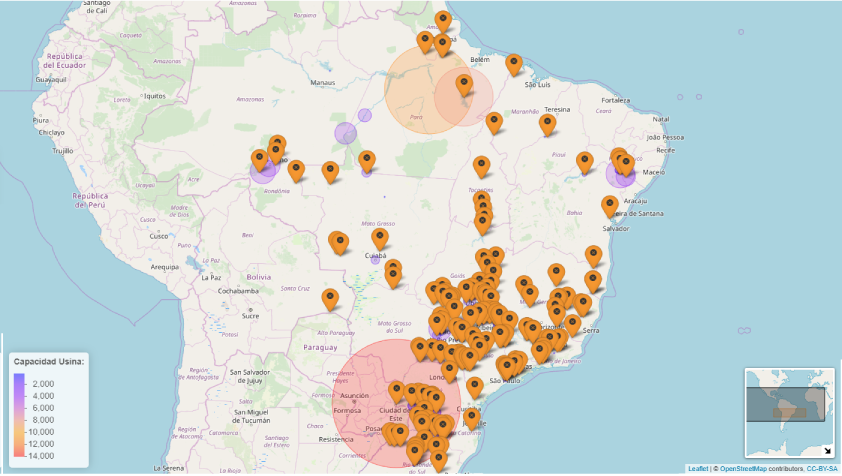
\includegraphics[scale=0.5]{map_estacVz}
	\caption{Estaciones de Medición de Caudales}\label{fig:mapa_vaz}
\end{figure}



\item Por otro lado, se tienen variables relacionadas al Clima, de frecuencia mensual, disponibles desde enero de 2000, hasta enero de 2017. Obtenidas del \href{http://www.inmet.gov.br/portal/}{Instituto Nacional de Meteorología (INMET)}. Se cuenta con observaciones de 4 variables siguientes en 265 estaciones georreferenciadas.

\begin{itemize}


\item Precipitación
\item Temperatura Máxima
\item Temperatura Mínima
\item Humedad Relativa Media


\end{itemize}

El link de descarga de estos datos es:

\url{http://www.inmet.gov.br/portal/index.php?r=bdmep/bdmep}


Se muestra en la figura \ref{fig:mapa_clm} la disposición de las estaciones de medición de variables climáticas.


\begin{figure}[H]
	\centering
	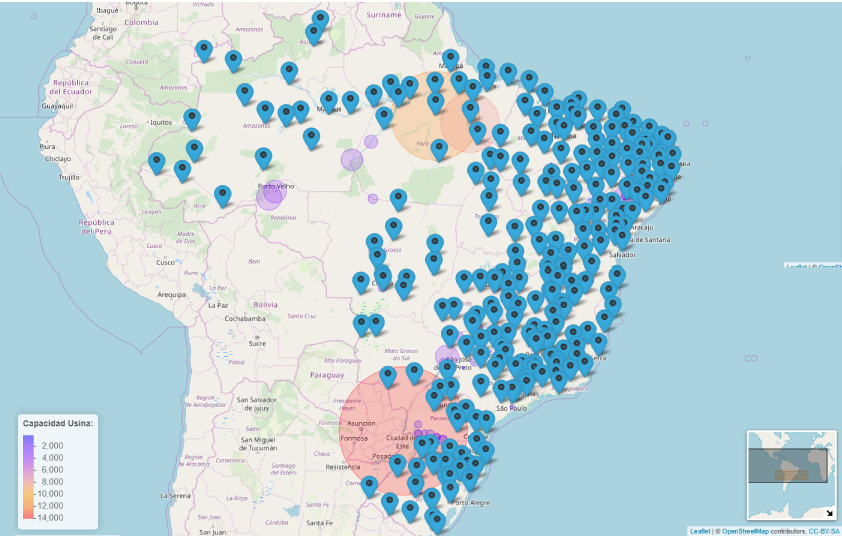
\includegraphics[scale=0.5]{map_estacClm}
	\caption{Estaciones de Medición de Variables Climáticas}\label{fig:mapa_clm}
\end{figure}

\end{enumerate}

\paragraph{Observación.} Para el modelamiento de las series de caudales se considera el periodo enero de 2000 a diciembre de 2015, ya que en este periodo se poseen datos tanto de caudales como de condiciones climáticas, mismas que se incluirán en un modelo SARIMAX como variables regresoras.

Cabe mencionar además que existen otras fuentes de datos, como \href{http://climexp.knmi.nl/start.cgi?id=someone@somewhere}{Climate Explorer}, en donde se puede encontrar información mensual (inclusive diaria) de índices globales de clima. Sin embargo, estas variables al no estar georeferenciadas, no se las incluye en el modelo planteado en capítulos posteriores.



%Capitulo2: Marco Teorico ............................
\chapter{Marco Teórico}



% 2.0 Series de Tiempo


% Intro del Capitulo (Marco Teorico)

En el presente capítulo, se definen las nociones y conceptos teóricos necesarios para comprender la metodología utilizada en la construcción de los modelos que proponemos para analizar los caudales de los ríos. Se empieza describiendo algunas estructuras de datos y sus respectivos objetos matemáticos asociados. Luego se muestra una propuesta para la limpieza de de datos asociados a series de tiempo basada en una técnica de descomposición conocida como STL-Loess. Luego se muestran definiciones que permitirán llevar acabo de manera adecuada el Análisis Clúster, es decir, la elección de la función de disimilitud y algoritmos de agrupamiento. Al final se muestra la metodología Box y Jenkins que se utilizará en la identificación y estimación de los modelos SARIMA y SARIMAX.


\section{Series de Tiempo}

Para el análisis de una variedad de fenómenos económicos o físicos se dispone, en general, de una cierta cantidad de observaciones, tomadas en momentos equidistantes. A una serie de observaciones de este tipo se le llama serie cronológica o temporal \cite{capa2016seriest}.
%La obvia correlación existente entre observaciones adyacentes en el tiempo puede restringir severamente la aplicabilidad de muchos de los métodos estadísticos convencionales, que dependen de la suposición de que las observaciones son independientes e idénticamente distribuidas. En ese sentido el análisis de series de tiempo conduce a problemas nuevos en el modelamiento estadístico y la inferencia \cite{shumway2017time}.
%El análisis de los datos experimentales asociados a series temporales conduce a problemas nuevos en el modelamiento estadístico y la inferencia. La obvia correlación existente entre observaciones adyacentes en el tiempo puede restringir severamente la aplicabilidad de muchos de los métodos estadísticos convencionales, que dependen de la suposición de que las observaciones son independientes e idénticamente distribuidas. El enfoque sistemático mediante el cual se responde a las preguntas matemáticas y estadísticas planteadas por estas correlaciones de tiempo se conoce comúnmente como análisis de series de tiempo \cite{shumway2017time}.
A continuación se detallan algunas definiciones y propiedades que permitirán formalizar estas nociones y profundizar en el análisis de este tipo de fenómenos.

\begin{definicion}
Un proceso estocástico es una colección de variables aleatorias $(Y_t , t\in T)$ parametrizada por un conjunto $T$ llamado espacio  de tiempos, en donde las variables toman valores en un conjunto $S$ llamado espacio de estados.
\end{definicion}

Usualmente se considera $T = \R$ o algún subconjunto de este, como $\N$ o $\Z$. De igual manera $S=\R$, aunque puede ser $\C$, $\R^k$ o inclusive $\C^k$.

\begin{definicion}
Una serie de tiempo es un proceso estocástico con espacio de tiempos $\Z$ y espacio de estados $\R$.
\end{definicion}




%%% Estacionariedad Fuerte --------------
\begin{definicion}
Un proceso $(Y_t, t\in \Z)$ se dice fuertemente estacionario si:

$$ \text{Distribución}(Y_{t_1+l},Y_{t_2+l},...,Y_{t_k+l}) =  \text{Distribución}(Y_{t_1},Y_{t_2},...,Y_{t_k}) $$

para $k=1,2,...$ y $t_1, t_2,..., t_k \in \Z$
\end{definicion}

% Segundo orden   ----------------------
\begin{definicion}
Un proceso real $(Y_t, t \in \Z)$ se dice de segundo orden si 
$$E(Y_t^2)<\infty$$ 
para todo $t\in\Z$.
\end{definicion}

% Estacionario  ------------------------
\begin{definicion}
Un proceso $(Y_t, t\in \Z)$ de segundo orden se dice estacionario si:
\begin{enumerate}
\item $E(Y_t)=c$
\item $Cov(Y_{s+l}, Y_{t+l})=Cov(Y_{s}, Y_{t})$ para todo $s,t,l\in \Z$
\end{enumerate}

\end{definicion}



%%% Autocovarianza ---------------------
\begin{definicion}
Dado un proceso estacionario $(Y_t, t \in \Z)$, se define la función de autocovarianza de este proceso, como sigue:
$$\gamma(k):=Cov(Y_t, Y_{t-k})$$
Para todo $k,t\in\Z$
\end{definicion}

Se puede demostrar que la función de autocovarianza cumple las siguientes propiedades:

\begin{itemize}
\item $V(Y_t)=\gamma(0)$
\item $\gamma(k) =  \gamma(-k) $
\item $|\gamma(k)| \leq  \gamma(0) $

\end{itemize}
 

%%% Autocorrelacion  -------------------
\begin{definicion}
La función de autocorrelación de un proceso estacionario $(Y_t, t\in \Z)$, se define por:
$$\rho(k):=\frac{\gamma(k)}{\gamma(0)}$$
\end{definicion}





%%% Correlacion Cruzada  -------------------
\begin{definicion}
La función de correlación cruzada de orden $k$ entre los procesos estacionarios $(X_t, t\in \Z)$ y $(Y_t, t\in \Z)$, se define como:
$$\rho_{xy}(k):=\frac{\gamma_{xy}(k)}{\sqrt{\gamma_x(0) \gamma_y(0) }}$$

Donde $\gamma_{xy}(k):=Cov(X_t,Y_{t-k})$, y no depende de $t$.

\end{definicion}







% Ruido Blanco  -------------------------
\begin{definicion}
Sea $(Y_t, t\in \Z)$ un proceso real de segundo orden, se conoce como ruido blanco (débil) si cumple las siguientes condiciones:

\begin{enumerat1e}
\item $E(Y_t)=0$
\item $V(Y_t)= \sigma^2 \geq 0$
\item $Cov(Y_t,Y_s)=0 , \text{ para } s\neq t, \forall t,s\in\Z$
\end{enumerate}

\end{definicion}

%Operador B backward and forward---------

\begin{definicion}
Llamaremos operador de retardo $B$ (Backward), a aquel operador que asocia a un proceso $(X_t,t\in\Z)$ el proceso $(Y_t,t\in\Z)$ donde:
$$Y_t = BX_t=X_{t-1}$$
Se puede demostrar que este operador es lineal e invertible, y su inverso $B^{-1}=F$ (Forward), también conocido como operador de avance, se define por:
$$F X_t = X_{t+1}$$
Además, para todo $n\in \N$ se satisface:
$$B^n X_t = X_{t-n}$$
$$F^n X_t = X_{t+n}$$
\end{definicion}




% 2.1 Descomposicion STL - Loess




\section{Descomposición STL - Loess}

STL es un procedimiento desarrollado por \citeauthor{cleveland1990stl} \citeyear{cleveland1990stl}, que permite descomponer una serie de tiempo en sus componentes estacional, tendencia y Residuo. STL tiene un diseño simple que consiste en una secuencia de aplicaciones del Loess Smoother; la simplicidad permite el análisis de las propiedades del procedimiento y permite un cálculo rápido, incluso para series de tiempo muy largas y con marcadas tendencias, así como estacionalidad. Otras características de STL son la capacidad de fijar el nivel de ``suavizado'' estacional (es decir, que tan suave es la curva asociada)} y de tendencias que varían, de manera casi continua, desde una cantidad muy pequeña de suavizado hasta una cantidad muy grande; estimaciones robustas de la tendencia y los componentes estacionales que no están distorsionados por un comportamiento aberrante en los datos; especificación del período de componente estacional a cualquier múltiplo entero del intervalo de muestreo de tiempo mayor que uno; y la capacidad de descomponer series de tiempo con valores perdidos.

\subsection*{Definiciones}

\subsection{Loess-Regresión Local}
\label{sec:loess}
Sean $x_i$ y $y_i$ (para $i = 1,2,...,n$) observaciones de una variable independiente y dependiente respectivamente. La curva de regresión   ``Loess'', $\hat{g}(x)$, es un suavizado de $y$ dado $x$ que puede calcularse para cualquier valor de dominio de la variable independiente. Así Loess está definida sobre cualquier valor no solamente sobre $x_i$. Como se verá más adelante, esta es una importante característica que permitirá lidiar con los valores perdidos y eliminar el componente estacional de manera sencilla.
En realidad Loess puede ser usada para suavizar $y$ en función de cualquier número de variables independientes, pero para STL, solo es necesario considerar una variable independiente.

Primero se calcula $\hat{g}(x)$ de la siguiente manera. Se escoge un entero positivo $q$. Supongamos $q\leq n$. Los $q$ valores de $x_i$ que son más cercanos a $x$ se seleccionan, cada uno está dado por el \textit{Peso del Vecindario} basado en su  distancia desde $x$. Sea $\lambda_q(x)$ la distancia del \textit{q-ésimo} $x_i$ más lejano de $x$. Sea $W$ la función de peso tricúbica definida por:
\[
W(u)=
\left\{\begin{matrix}
(1-u^3)^3 & \text{para } 0\leq u < 1  \\ 
0 & \text{para } u\geq 1
\end{matrix}\right.
\] 

El peso del vecindario para cualquier $x_i$ es 

$$ v_i(x)=W \left( \frac{|x_i-x|}{\lambda_q(x)} \right) $$

Así un $x_i$ cercano a $x$ tiene el peso más grande; los pesos decrecen a medida que $x_i$ se aleja de $x$, mientras que se aproxima a cero en el \textit{q-ésimo} punto más lejano. El próximo paso es ajustar un polinomio de grado $d$ a los datos con peso $v_i(x)$ en $(x_i,y_i)$. El valor del polinomio ajustado localmente evaluado en $x$ es $\hat{g}(x)$. En este caso solo se analiza el caso en que $d=1$ y $2$, es decir, ajustando localmente un polinomio lineal o cuadrático.

Ahora suponiendo que $q>n$. $\lambda_n(x)$ es la distancia de $x$ al $x_i$ más lejano. Para $q>n$ se define $\lambda_q(x)$ por
$$\lambda_q(x)=\lambda_n(x)\frac{q}{n}$$

Luego de manera análoga a lo anterior, se definen los pesos de los vecindarios usando este valor de $\lambda_q(x)$.

Para usar Loess, $d$ y $q$ deben ser previamente elegidos. Las elecciones en el contexto de STL se discutirán a detalle más adelante. A medida que $q$ crece, $\hat{g}(x)$ se hace más suave. Cuando $q$ tiende a infinito, $v_i(x)$ tiende a 1 y $\hat{g}(x)$ tiende al polinomio de mínimos cuadrados ordinarios de grado $d$.

Suponiendo que cada observación $(x_i,y_i)$ tiene un peso $\rho_i$ que expresa la confianza de la observación relativa a las otras. Por ejemplo, si $y_i$ tiene varianza $\sigma^2k_i$ donde $k_i$ es conocido, luego $\rho_i$ puede ser $1/k$. Así, se pueden incorporar estos pesos en el suvizamiento Loess en forma sencilla usando $\rho_i v_i(x)$ como los pesos en el ajuste de mínimos cuadrados. Esto provee un mecanismo mediante el cual se puede construir robustez en STL.

\subsubsection{El diseño general.}

STL consiste de dos procedimientos recursivos: un bucle interno anidado dentro de un bucle externo. En cada uno de los pasos del bucle interno, las componentes de tendencia y estacionalidad son actualizadas una vez; cada recorrido completo del bucle interno consiste de $n_{(i)}$ iteraciones. Cada paso del bucle externo consiste del bucle interno seguido por el cálculo de pesos de robustez; estos pesos son usados en la siguiente corrida del bucle interno para reducir la influencia del comportamiento transitorio y aberrante en las componentes de tendencia y  estacionalidad. Un paso inicial del bucle externo se realiza con todos los pesos de robustez iguales a 1, y luego $n_{(0)}$ pasos del bucle externo se llevan acabo. Las elecciones de $n_{(i)}$ y $n_{(0)}$ se discutirán más adelante. 

Suponiendo que el número de observaciones en cada periodo, o ciclo, de la componente estacional es $n_{(p)}$. Por ejemplo, si la serie es mensual con un año de periodicidad, entonces $n_{(p)}=12$. Es necesario poder referirnos a la subserie de valores en cada posición del ciclo estacional. Por ejemplo, para una serie mensual con $n_{(p)}=12$, la primera subserie contiene los valores de Enero, la segunda tiene los valores de Febrero, y así sucesivamente. Se referiran a cada una de estas $n_{(p)}$ subseries como \textit{subserie-ciclo}.

\subsection{Bucle Interno}

Cada paso de el bucle interno consiste de un suavizado estacional que actualiza la componente estacional, seguida por suavizado de tendencia que actualiza la componente de tendencia. Suponiendo $S_v^{(k)}$ y $T_v^{(k)}$ para $v=1,2,...,N$ son las componentes estacional y de tendencia al final del \textit{k-ésimo} paso; estas dos componentes se definen para todos los tiempos $v=1,2,...,N$, inclusive donde $Y_v$ es un valor perdido. Las actualizaciones de el $(k+1)$ paso, $S_v^{(k+1)}$ y $T_v^{(k+1)}$, son calculadas de la siguiente manera:

\subsubsection{Paso 1.} \textit{Quitar Tendencia.-}
\label{sbsec:paso1}
Se calcula la serie $Y_v-T_v^{(k)}$ que no tiene tendencia . Si $Y_v$ tiene un valor perdido en un punto particular del tiempo, entonces la serie sin tendencia tiene también un valor perdido en esa posición.

\subsubsection{Paso 2.} \textit{Suavizar Subseries Ciclo.-}
\label{sbsec:paso2}
Cada subserie-ciclo de la serie sin tendencia es suavizado mediante Loess considerando $q=n_{(s)}$ y $d=1$. Los valores suavizados se calculan en todas las posiciones de tiempo de las subseries-ciclo, incluyendo aquellos con valores perdidos, y en las posiciones justo antes de la primera posición de la subserie y justo después del último. Por ejemplo, suponga que la serie es mensual, $n_{(p)}=12$. La colección de los valores suavizados para todas las subseries-ciclo son series estacionales provisionales, $C_v^{(k+1)}$, consiste de $N+2n_{(p)}$ valores que van desde $v=-n_{(p)}+1$ hasta $N+n_{(p)}$.  

\subsubsection{Paso 3.} \textit{Paso-bajo Filtro de Suavizado de Subseries Ciclo.-}
\label{sbsec:paso3}
Un filtro paso-bajo es aplicado a $C_v^{(k+1)}$. El filtro consiste de una media móvil de longitud $n_{(p)}$, seguido por otra media móvil de longitud $n_{(p)}$, seguida de una media móvil de longitud $3$, seguida de un suavizado Loess con $d=1$ y $q=n_{(l)}$. La salida. $L_v^{(k+1)}$, esta definida en las posiciones $v=1$ hasta $N$ porque las tres medias móviles no pueden extenderse hasta el final. El suavizado estacional \ref{sbsec:paso2}  fue extendido $n_{(p)}$ posiciones en cada final en anticipación de esta pérdida.

\subsubsection{Paso 4.} \textit{Quitar tendencia de las Subseries Ciclo suavizadas.-}
\label{sbsec:paso4}
El componente estacional desde el $(k+1)$ \textit{-ésimo} bucle es $S_v^{(k+1)}=C_v^{(k+1)}-L_v^{(k+1)}$ para  $v=1,2,...,N$. Se resta $L_v^{(k+1)}$ para evitar que perturbaciones de baja frecuencia entre en la componente estacional.

\subsubsection{Paso 5.} \textit{Desestacionalización.-}
\label{sbsec:paso5}
Se calcula la serie desestacionalizada $Y_v-S_v^{(k+1)}$. Si $Y_v$ es un dato perdido en una posición particular de tiempo, entonces también lo será en la serie desestacionalizada.

\subsubsection{Paso 6.} \textit{Suavizado en Tendencia.-}
\label{sbsec:paso6}
La serie desestacionalizada es suavizada mediante Loess con los parámetros $q=n_{(t)}$ y $d=1$. Los valores suavizados se calculan para todas las posiciones de tiempo $(v=1,2,...,N)$, inclusive donde existen valores perdidos. La componente de tendencia del $(k+1)$ \textit{-ésimo} bucle, $R_v^{(k+1)}$ para $v=1,2,...,N$, es el conjunto de valores suavizados. 


Así la porción suavizada estacional del bucle interno corresponde a los pasos 2,3,y 4, mientras que la porción de suavizado en tendencia corresponde al \hyperref[sbsec:paso6]{Paso 6}

Para llevar a cabo el Paso 1 en el paso inicial a través del bucle interno es necesario definir valores iniciales, $T_v^{(0)}$, para la componente de tendencia. Usando $T_v^{(0)}=0$ funciona bastante bien. La tendencia se vuelve parte de la Subserie-Ciclo suavizada, $C_v^{(1)}$, pero se elimina en gran medida durante el 
\hyperref[sbsec:paso4]{Paso 4}.


\subsection{Bucle externo}
Se supone que se ha realizado una ejecución inicial del bucle interno para obtener estimaciones, $T_v$ y $S_v$, de la componentes de tendencia y estacionalidad. Luego el residuo es

$$R_v = Y_v - T_v - S_v$$

(Nótese que el residuo, a diferencia de $T_v$ y $S_v$, no está definido donde $Y_v$ tiene valores perdidos.) 
Se define un peso a cada posición de tiempo en la que $Y_v$ es observado. Estos \textit{pesos de robustez} reflejan lo extremo que es $R_v$. Un valor atípico en los datos que resultan en un $|R_v|$ muy grande tendrá un peso pequeño o próximo a cero. Sea
$$h=6 \text{ mediana}(|R_v|)$$

Luego los pesos de robustez en el tiempo $v$ son:
$$\rho_v=B \left( \frac{|R_v|}{h}  \right)$$

Donde $B$ es la función bicuadrática de pesos:
\[
B(u)=
\left\{\begin{matrix}
(1-u^2)^2 & \text{para } 0\leq u < 1  \\ 
0 & \text{para } u\geq 1
\end{matrix}\right.
\] 

Ahora el bucle interno se repite, pero en las series suavizadas de los \hyperref[sbsec:paso2]{Paso 2} y \hyperref[sbsec:paso6]{Paso 6}, el peso del vecindario para el valor en el tiempo $v$ se multiplica por el peso de robustez, $\rho_v$. Esto es solo un uso de los pesos de confiabilidad discutidos en la \hyperref[sec:loess]{Loess}. Estas iteraciones de robustez del bucle externo se llevan a cabo un total de $n_{(0)}$ veces. Cada vez que se ingresa al bucle interno después de la pasada inicial no se fija $T_v^{(0)}$ como se hizo en la pasada inicial, sino se usa el componente de tendencia del \hyperref[sbsec:paso6]{Paso 6} del bucle interno anterior.

\subsection{Elección de Parámetros}

Como se nota en la sección anterior, STL necesita de la especificación de los 6 parámetros siguientes:
\begin{itemize}
\item $n_{(p)}=$ Número de observaciones en cada ciclo de la componente estacional,
\item $n_{(i)}=$ Número de iteraciones a través del bucle interno,
\item $n_{(o)}=$ Número de iteraciones robustas del bucle externo,
\item $n_{(l)}=$ Parámetro de suavizado para el filtro del paso inferior,
\item $n_{(t)}=$ Parámetro de suavizado para la componente de tendencia,
\item $n_{(s)}=$ Parámetro de suavizado para la componente estacional.
\end{itemize}

%La elección de los \textcolor{red}{5 primeros} parámetros es sencilla. Sin embargo, $n_{(s)}$ debe elegirse cuidadosamente para cada aplicación. 


El parámetro $n_{(p)}$ indica la periodicidad de la serie, por ejemplo para datos diarios de con periodicidad anual se toma $n_{(p)}=365$, mientras que si los datos son mensuales como en nuestro caso se tomará $n_{(p)}=12$.
Para escoger los demás parámetros \citeauthor{cleveland1990stl} \citeyear{cleveland1990stl} recomiendan elegirlos de la siguiente manera:

\begin{enumerate}
\item $n_{(l)}= [n_{(p)}]_{impar}$ , es decir, el menor entero impar mayor que $n_{(p)}$.
\item $n_{(s)}$, debe ser un impar mayor o igual que 7.
\item $n_{(t)} = [ 1.5n_{(p)}/(1-1.5/n_{(s)})]_{impar}$
\item Si no es necesario que las iteraciones sean robustas usar $n_{(i)}=2$ y $n_{(o)}=0$. Pero si se desea robustez se debe tomar $n_{(i)}=1$ , y $n_{(o)}=5$, aunque para asegurar la convergencia del método se puede tomar $n_{(o)}=10$.
\end{enumerate}


%%%%%%%%%%%%%%%%%%%%%%%%%%%%%%%%%%%%%%%%%%%%%%%%%%%%

%Para la elección de $n_{(i)}$ primero supongamos que no necesitamos las iteraciones robustas ($n_{(p)}=0$), entonces se quiere escoger $n_{(i)}$ suficientemente grande para que las actualizaciones de las componentes estacional y de tendencia \textcolor{red}{converjan.} Afortunadamente en la práctica se ha demostrado que convergen bastante rápido \cite{cleveland1990stl}, por lo que en la mayoría de los casos basta tomar $n_{(i)}=1$, \textcolor{red}{aunque \citeauthor{cleveland1990stl} recomiendan tomar $n_{(i)}=2$.}

%En el caso en que necesitemos las iteraciones robustas, se elige $n_{(o)}$ lo suficientemente grande para que las estimaciones de las componentes estacional y de tendencia converjan, por lo que \citeauthor{cleveland1990stl} sugiere fijar $n_{(0)}=5$.

%\subsubsection{$n_{(l)}$, parámetro de suavizado para el filtro del paso inferior}

%$n_{(l)}$ siempre se toma como el menor entero impar mayor que $n_{(p)}$.

%Para elegir $n_{(s)}$, notamos que cada subserie ciclo se suaviza a medida que $n_{(s)}$ crece, otro criterio a considerar es que $n_{(s)}$ debe ser un impar mayor o igual que 7.

%El valor que sugiere \textcolor{red}{....?(1990)} para $n_{(t)}$ es:
%$$  n_{(t)} = \left[  \frac{1.5n_{(p)}}{(1-1.5n_{(s)})}   \right]_{impar} $$


%%%%%%%%%%%%%%%%%%%%%%%%%%%%%%%%%%%%%%%%%%%%%%%%%%%%%%%%%%



















% 2.2 Limpieza de Series de Tiempo

\section{Tratamiento de Valores perdidos}
\label{sec:limpieza}
El tratamiento de valores perdidos en una base de datos es un procedimiento fundamental en cualquier estudio estadístico, debido a que puede provocar en cierta medida un impacto sobre los resultados obtenidos del estudio.

En esta sección se ilustra una propuesta para el tratamiento de valores perdidos en series de tiempo estacionales. Para ello se considera una serie de tiempo $(Y_t,t\in \Z)$, de la que se conocen las observaciones 
$$y_1,y_2,...,y_{j-1}, y_j, y_k, y_{k+1},...,y_n$$

donde $1 < j < k < n$, es decir, no se conocen los valores de $y_t$ para $t=j+1, j+2, ..., k-1$. Se considera este caso, en el que existe un periodo, compuesto de instantes consecutivos, en el que no se conoce el valor de $y_t$, pero se ve que a partir de este es posible extender el método para tratar a series de tiempo con varios periodos o inclusive instantes no consecutivos de tiempo.

Como se ve en la sección anterior, la descomposición STL-Loess permite descomponer aditivamente una serie de tiempo en sus componentes de tendencia y estacionalidad inclusive en aquellos valores de $t$ para los que no se conoce $y_t$. Entonces se aplica la descomposición STL-Loess a $Y_t$, así se obtiene su tendencia $T_t$ y estacionalidad $S_t$ en todo instante de tiempo $t=1,2,...,n$. Además, se obtiene un residuo $U_t$ en aquellos instantes de tiempo $t$ en los cuales se conoce $Y_t$, es decir para $t=1,2,...,j,k,...,n$.


\begin{equation}
\label{eq:stl_descomp}
Y_t = T_t + S_t + R_t
\end{equation}

Se ilustra lo antes mencionado en la figura \ref{fig:stl_descomp}, que corresponde a la descomposición STL-Loess de una serie de datos mensuales de precipitación (lluvias) medidos en cierta zona de Brasil, está serie tiene estacionalidad anual (12 meses); nótese que es necesario fijar los parámetros de la descomposición adecuadamente ya que están asociados al número de retardos considerados al estimar tanto la componente estacional como la tendencia. El gráfico muestra en la primera fila la serie climática, en segundo lugar muestra su componente estacional, en tercera fila se encuentra su componente de tendencia, y finalmente el residuo. Como se puede notar las componentes de tendencia y estacionalidad están definidas en todo el dominio de tiempo.

\begin{figure}[h]
\caption{Descomposición STL-Loess de Serie}
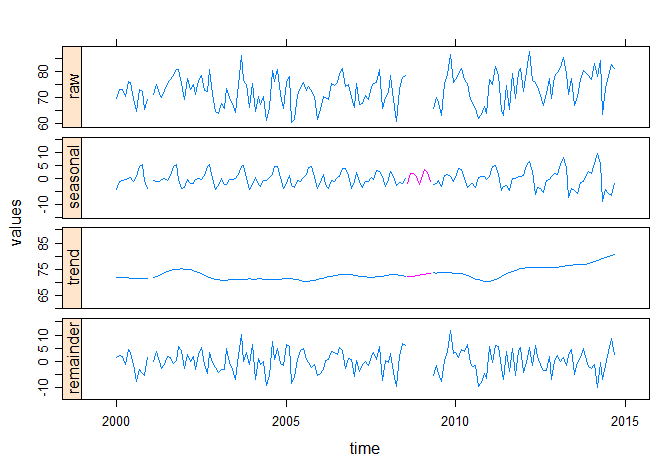
\includegraphics[width=15cm]{Cap2-Stl-Loess.png}
\label{fig:stl_descomp}
\centering
\end{figure}

Es decir, bastaría conocer los valores de $R_t$ en todo instante $t$ e inmediatamente se conocería los valores de $Y_t$ de inmediato a partir de la ecuación \eqref{eq:stl_descomp}.


Así, se propone simular los valores perdidos de $R_t$. Una forma simple de simular dichos valores, es usando la función de distribución empírica de los Residuos, y el método simulación de la ``Transformada Inversa''. Esto debido a que los residuos tienden a comportarse como un proceso estacionario, razón por la cual su distribución es invariante en el tiempo (conservando su media y varianza constantes), suponiendo que se especificaron bien los parámetros de la descomposición STL.


Pues bien, se propone el siguiente algoritmo de simulación de valores perdidos de $Y_t$.

\subsubsection{Algoritmo}

\begin{enumerate}
\item Primero se calcula la descomposición STL de $Y_t$. Así se obtiene:
\begin{itemize}
\item $T_t$, y $S_t$ para $t=1,2,...,n$
\item $R_t$ para $t=1,2,...,j-1,j,k,k+1,...,n$
\end{itemize}


\item Luego se calcula la función de distribución empírica $\hat{F}_0(u)$ de los residuos conocidos $R_t$.

$$\hat{F}_0(u):=\frac{1}{n}\sum_{i\in J} \indic_{(R_i\leq u)} $$
Donde $J=\{1,2,...,j-1,j,k,k+1,...,n\}$

\item Usando el método de la Transformada Inversa \cite{ross2006simulation}. Para $t$ desde $j+1$ hasta $k-1$ (instantes en los que se tiene valores perdidos), hacer lo siguiente:

\begin{itemize}
\item Simular $u\sim U[0,1]$
\item Calcular $$r = \hat{F}_0^{-1}(u) := inf\{ t\in \mathbb{R}: u\leq \hat{F}_0(t) \} $$
\item Definir $R_t := r$
\item Calcular $Y_t:=T_t+S_t+R_t$
\end{itemize}

\end{enumerate}


Volviendo al ejemplo antes mostrado \ref{fig:stl_descomp}, luego de aplicar el algoritmo de simulación de valores perdidos se obtiene la serie completa $Y_t$ como se puede observar en la figura \ref{fig:stl_descomp2}.

\begin{figure}[h]
\caption{Serie Corregida}
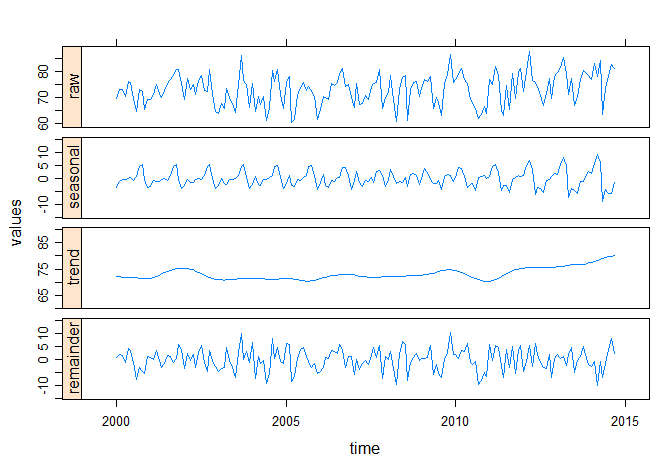
\includegraphics[width=15cm]{Cap2-MarcoTeorico/Cap2-Stl-Loess2.png}
\label{fig:stl_descomp2}
\centering
\end{figure}












% 2.3 Funciones de Disimilitud entre TS's 

\section{Análisis de Conglomerados (Clúster)}


%El Análisis Clúster es un técnica de aprendizaje no supervisada que tiene como objetivo dividir un conjunto de objetos en grupos homogéneos (clústers). La partición se realiza de tal manera que los objetos en el mismo clúster son más similares entre sí que los objetos en diferentes grupos según un criterio definido. En muchas aplicaciones reales, el análisis de clúster debe realizarse con datos asociados a  series de tiempo. De hecho, los problemas de agrupamiento de series de tiempo surgen de manera natural en una amplia variedad de campos, incluyendo economía, finanzas, medicina, ecología, estudios ambientales, ingeniería y muchos otros. 
%Con frecuencia, la agrupación de series de tiempo desempeña un papel central en el problema estudiado. Estos argumentos motivan el creciente interés en la literatura sobre la agrupación de series de tiempo, especialmente en las últimas dos décadas, donde se ha proporcionado una gran cantidad de contribuciones sobre este tema. En \cite{liao2005clustering} se puede encontrar un excelente estudio sobre la agrupación de series de tiempo, aunque posteriormente se han realizado nuevas contribuciones significativas. Particularmente importante en la última década ha sido la explosión de documentos sobre el tema provenientes tanto de comunidades de minería de datos como de reconocimiento de patrones. \cite{fu2011review} proporciona una visión general completa y exhaustiva de las últimas orientaciones de minería de datos de series de tiempo, incluida una gama de problemas clave como representación, indexación y segmentación de series de tiempo, medidas de disimilitud, procedimientos de agrupamiento y herramientas de visualización.

%Una pregunta crucial en el Análisis Clúster es establecer lo que queremos decir con objetos de datos "similares", es decir, determinar una medida de similitud (o disimilitud) adecuada entre dos objetos. En el contexto específico de los datos asociados a series de tiempo, el concepto de disimilitud es particularmente complejo debido al carácter dinámico de la serie. Las diferencias generalmente consideradas en la agrupación convencional no podrían funcionar adecuadamente con los datos dependientes del tiempo porque ignoran la relación de interdependencia entre los valores. 

%De esta manera, diferentes enfoques para definir una función de disimilitud entre series de tiempo han sido propuestos en la literatura pero nos centraremos en aquellas medidas asociadas a la autocorrelación (simple, e inversa), correlación cruzada y periodograma de las series \cite{struzik1999haar};  \cite{galeano2000multivariate}; \cite{caiado2006periodogram}; \cite{chouakria2007adaptive}. Estos enfoques basados en características tienen como objetivo representar la estructura dinámica de cada serie mediante un vector de características de menor dimensión, lo que permite una reducción de dimensionalidad (las series temporales son esencialmente datos de alta dimensionalidad) y un ahorro significativo en el tiempo de cálculo, además de que nos ayudan a alcanzar el objetivo central por el que usaremos el Análisis Clúster que es el de la modelización de series de tiempo.

El análisis de Conglomerados o Clúster es una rama de métodos que tienen el objetivo de agrupar un conjunto de objetos de tal manera que los objetos de cada grupo sean los más ``similares'' posible, mientras que objetos de distintos grupos sean ``distintos''. Una etapa fundamental de este análisis corresponde a la especificación de una medida de similitud (o disimilitud) que permita cuantificar que tan similares o distintos son los objetos analizados.

%%%%%%%%%%%%%%%%%%%%%%%%%%%%%%%%%%%%%%%%%%%%%%%%

%El análisis de Conglomerados o Clúster es una rama de métodos que tienen el objetivo de agrupar un conjunto de objetos de tal manera que los objetos de cada grupo sean los más "similares" posible, mientras que objetos de distintos grupos sean "distintos". Una etapa fundamental de este análisis corresponde a la especificación de una medida de similitud (o disimilitud) que permita cuantificar que tan "similares" o "distintos" son los objetos analizados.

\subsection{Métricas y Funciones de Disimilitud}

Desde un punto de vista general el término proximidad indica el concepto de cercanía en espacio, tiempo o cualquier otro contexto. Desde un punto de vista matemático, ese término hace referencia al concepto de disimilitud o similaridad entre dos elementos. 
Sea O un conjunto finito o infinito de elementos (individuos, estímulos, sujetos u objetos sobre los que se quiere definir una proximidad).


\begin{defin}
Dados $O_i, O_j \in O$ y $\delta$ es una función real de $O \times O \rightarrow \mathbb{R}$, con $\delta_{ij}:=\delta(O_i,O_j)$. Se dirá que $\delta$ es una disimilitud o función de disimilitud si verifica las siguientes condiciones:
\begin{itemize}
\item $\delta_{ij}=\delta_{ji}$, $\forall i,j$
\item $\delta_{ii} \leq \delta_{ij}$, $\forall i,j$
\item $\delta_{ii}= c$, $\forall i$
\end{itemize}
\end{defin}

La primera condición podría eliminarse, aunque resulta necesaria si se desea comparar con una distancia. No obstante, esa condición suele violarse cuando la disimilitud proviene de juicios emitidos por sujetos, ya que éstos no siempre califican igual al par $(O_i,O_j)$ que al par $(O_j,O_i)$. Las condiciones segunda y tercera suelen establecerse igualmente para $\delta_o=0$, aunque también es conocido que cuando a un individuo le son presentados dos objetos idénticos, éste tiende a asignarles algún valor de disimilitud no nulo y generalmente positivo, y además no siempre se define $c \geq 0$ ya que, si por ejemplo las disimilitud provienen de una transformación, éstas podrían ser negativas.

Existen diferentes medidas para el cálculo de disimilitud entre un par de variables o individuos. Si se considera una matriz de datos $X=(x_{tj})_{n\times p}$, obtenida de $n$ objetos sobre $p$ vatiables, algunos ejemplos de medidas son:

\begin{itemize}
\item \textit{Distancia euclídea ponderada}
$$ \delta_{ts}=\left(\displaystyle \sum_{j=1}^p w_i(x_{tj}-x_{sj}) \right)^{1/2} $$
\item \textit{Métrica de Minkowski}
$$ \delta_{ts}=\left(\displaystyle \sum_{j=1}^p |x_{tj}-x_{sj}|^{\lambda}\right)^{1/\lambda}, \ \ \lambda \geq 1 $$
\item \textit{Separación angular}
$$ \delta_{ts}=1-\frac{\sum_{j=1}^p x_{tj}x_{sj}}{(\sum_j x_{tj}^2 \sum_j x_{sj}^2)^{1/2}} $$

\end{itemize}


\subsection{Métricas para Series de Tiempo}
\label{sec:metrica}
El problema de medir similitudes o diferencias entre datos asociados a series de tiempo ha sido estudiado ampliamente por autores como \citeauthor{johnson2004multivariate} \citeyear{johnson2004multivariate}, además de \citeauthor{galeano2000multivariate} \citeyear{galeano2000multivariate} propusieron comparar las funciones de autocorrelación de las series, \citeauthor{diggle1991nonparametric} \citeyear{diggle1991nonparametric} con enfoques no paramétricos comparó el espectro de las series,  \citeauthor{piccolo1990distance} \citeyear{piccolo1990distance} dió una métrica basada en modelos ARIMA, \citeauthor{diggle1997spectral} \citeyear{diggle1997spectral} desarrolló métodos basados en análisis espectral, y \citeauthor{maharaj2000cluster} \citeyear{maharaj2000cluster} comparó dos series estacionarias basándose en sus parámetros autoregresivos . A continuación se detallan dos de las métricas que se utilizan en nuestro análisis.

\begin{itemize}
\item  \citeauthor{galeano2000multivariate} \citeyear{galeano2000multivariate} propone una métrica que se basa en la estimación de la función de autocorrelación de las series. Sean $(X_t, t\in\Z)$, $(Y_t, t\in\Z)$ dos series de tiempo, y $\hat\rho_x$, $\hat\rho_y$  sus vectores de coeficientes de autocorrelación estimados hasta el retardo $k$ (que se supondrá, es el mayor retardo significativo). Así, se define la distancia como sigue:

$$d_{ACF}(X_t,Y_t) = \sqrt{(\hat\rho_x - \hat\rho_y)'\Omega (\hat\rho_x - \hat\rho_y)}$$
Donde $\Omega$ es una matriz de pesos, simétrica y semidefinida positiva (usualmente $\Omega=I_k$), que se puede utilizar para dar ponderaciones a los coeficientes que decrecen según el retardo. Esta métrica está relacionada con el enfoque paramétrico, ya que los parámetros de la aproximación autorregresiva de las series se calculan a partir de los coeficientes de autocorrelación de las mismas.



%\citeauthor{piccolo1990distance}
\item \citeauthor{corduas2008time} \citeyear{corduas2008time} definen a partir de trabajos previos como \citeauthor{piccolo1990distance} \citeyear{piccolo1990distance}, una métrica para series de tiempo que se pueden representar como un proceso de media cero invertible $ARIMA(p,d,q)$. Es decir:
$$\varphi_p (B) \Delta^d  X_t = \theta_q (B)\varepsilon_t $$

Al ser invertibles las series pueden escribirse en su forma Autoregresiva AR($\infty$) mediante el operador en retardos $$\pi_x(B) =  \frac{\theta_q (B) }{\varphi_p (B) }  = 1-\sum_{j=1}^\infty \pi_{xj} B^j $$
bajo esas condiciones, se define la métrica siguiente:

$$d_{PIC}(X_t,Y_t)= \sqrt{\sum_{j=1}^{\infty}(\pi_{xj}-\pi_{yj})^2$$

Que es la distancia euclídea entre los coeficientes de las representaciones $AR(\infty)$ de las dos series. Esta distancia $d_{PIC}$ es una medida bien definida debido a la convergencia absoluta de las series $\pi_x(B)$ y $\pi_y(B)$  de los procesos que pertenecen a una clase admisible ARIMA, y satisface las propiedades de una métrica. Además, tiene una interpretación interesante en términos de la función de pronóstico de un proceso lineal, que simplemente está determinado por los valores pasados de la serie y los coeficientes de $\pi(B)$ . Por lo tanto, la distancia entre dos procesos ARIMA, con órdenes dadas, es cero si, con el mismo conjunto de valores iniciales, los modelos correspondientes producen los mismos pronósticos.
Cabe mencionar que la distancia $d_{PIC}$ no toma en cuenta la varianza del ruido blanco asociado, esta se considera únicamente un factor de escala que depende de la unidad de medida y que no afecta a la estructura temporal del proceso. Además, hallar la distancia supone conocer a priori la representación ARIMA de las series.

\end{itemize}







%%%%%%%%%%%%%%%%%%%%%%%%%%%%%%%%%%%%%%%%%%%%%%%%%%%%%%%%%%%%%%%%%%%%%%

\subsection{Escalonamiento Multidimensional (MDS)}


El escalamiento multidimensional, conocido como MDS por sus siglas en inglés, engloba un conjunto de técnicas multivariantes desarrolladas en el ámbito del comportamiento, que persiguen el estudio de la estructura subyacente de un conjunto de objetos, es decir, que pretende representar un conjunto de objetos en un espacio de baja dimensionalidad. La palabra objeto es muy genérica y se refiere, en realidad, a cualquier entidad que se desee comparar, en este caso particular se considera a una series de tiempo. Los modelos y métodos de construcción de escalas multidimensionales fueron desarrollados en la mitad del siglo XX, entre los que cabe citar los trabajos de \citeauthor{stevens1946theory} \citeyear{stevens1946theory}, \citeauthor{coombs1950psychological} \citeyear{coombs1950psychological}, \citeauthor{torgerson1958theory} \citeyear{torgerson1958theory}, \citeauthor{kruskal1964multidimensional} \citeyear{kruskal1964multidimensional}, y \citeauthor{guttman1968general} \citeyear{guttman1968general}, que constituyen los antecedentes de los modelos y métodos más modernos de escalamiento multidimensional que pueden considerarse como generalizaciones de los primeros.




En términos generales, el Escalamiento Multidimensional permite representar en un espacio geométrico las proximidades entre pares de objetos a través de distancias (o disimilitudes) en función de un determinado número de dimensiones. Así, el MDS cumple su objetivo en dos etapas. En primer lugar, determina las dimensiones subyacentes más relevantes (normalmente entre 2 y 4). En segundo lugar, construye una representación geométrica de los datos a través de las distancias entre los mismos en las dimensiones relevantes.  De esta forma, el MDS asume un paralelismo entre el concepto psicológico de similaridad y el concepto geométrico de distancia.


% El escalamiento multidimensional opera sobre una matriz, cuyos elementos representan  disimilitudes entre un conjunto de objetos, con el objetivo de construir coordenadas de puntos, en un número predeterminado de dimensiones ($\R^2$ usualmente), de tal manera que la matriz de distancias entre estos puntos es aproximadamente la misma que la matriz de disimilitudes.
% Los modelos y métodos de construcción de escalas unidimensionales fueron desarrollados en la primera mitad del siglo XX, entre los que cabe citar a Thurstone, Likert, Guttman o Coombs, constituyen los antecedentes de los modelos y métodos más modernos de escalamiento multidimensional que pueden considerarse como generalizaciones de los primeros.

A continuación se muestra el plantemiento de está técnica en un contexto general, no se profundiza en ella ya que se usará unicamente para representar sobre un plano bidimensional a las series de tiempo asociadas a estaciones de medición de caudales, a partir de su matriz de disimilitudes. Se puede encontrar esta técnica, sus variantes y extensiones detalladas en trabajos como los de \citeauthor{borg2003modern} \citeyear{borg2003modern} y \citeauthor{cox2000multidimensional} \citeyear{cox2000multidimensional}.

\subsubsection{Modelo General MDS }

De modo general, se puede decir que el MDS toma como entrada una matriz de proximidades $\mathcal{D} \in M_{n \times n}$ (disimilitudes entre objetos), donde $n$ es el número de objetos. Cada elemento $\delta_{ij}$ de $\mathcal{D}$ representa la disimilitud entre un objeto $O_i$ y el objeto $O_j$.

$$ \mathcal{D} = \begin{pmatrix}
\delta_{11} & \delta_{12} & \cdots & \delta_{1n} \\
\delta_{21} & \delta_{22} & \cdots & \delta_{2n} \\
\vdots & \vdots &  \ddots & \vdots \\
\delta_{n1} & \delta_{n2} & \cdots & \delta_{nn} \\
\end{pmatrix} $$

A partir de esta matriz de proximidades, el MDS proporciona como resultado una matriz $X \in M_{n \times m}$, representación $m$-dimensional de los $n$ objetos. Cada valor $X_{ik}$ representa la coordenada $k$ del objeto $i$, para $i=1,2,...,n$. 

$$ X= \begin{pmatrix}
X_{11} & X_{12} & \cdots & X_{1m} \\
X_{21} & X_{22} & \cdots & X_{2m} \\
\vdots & \vdots &  \ddots & \vdots \\
X_{n1} & X_{n2} & \cdots & X_{nm} \\
\end{pmatrix} $$


La matriz $X$ se busca de tal manera que su matriz de distancias $D(X) = (d_{ij})_{n\times n}$, considerando la métrica euclidea sobre $\R^m$, se aproxime lo más posible a la matriz de proximidades $\mathcal{D}$.

$$ d_{ij}:=\left[\displaystyle \sum_{k=1}^m (X_{ik}-X_{jk})^2 \right]^{1/2} \text{ , para } i,j=1,2,...,m$$


Existen distintos enfoques desde los cuales se puede hallar $X$, uno de ellos consiste de hallar valores y vectores propios de una matriz asociada a $D(X)$. Se resume el método para hallar $X$ en el siguiente algoritmo:

\begin{enumerate}

\item Calcular la matriz $A=(a_{ij})_{n\times n}$ , donde $a_{ij} = -\frac{1}{2}\delta_{ij}^2$
\item Calcular la matriz $B = (b_{ij})_{n\times n}$ , donde: 

$$b_{ij} = a_{ij} -a_{i*}-a_{*j} + a_{**} $$
$$a_{i*} = \frac{1}{n} \sum_{j=1}^n a_{ij}  $$
$$a_{*j} = \frac{1}{n} \sum_{i=1}^n a_{ij}  $$
$$a_{**} = \frac{1}{n^2} \sum_{j=1}^n  \sum_{i=1}^n  a_{ij}  $$

\item Hallar los valores propios de $B$, $\lambda_1, \lambda_2, \dots , \lambda_{n-1}$ y sus respectivos vectores propios $v_1, v_2, \dots, v_{n-1}$ normalizados de tal manera que $v_k' v_k = \lambda_k$ para $k=1,\dots,n-1$. Si $B$ no es semidefinida positiva (posee algun valor propio negativo), se puede ignorar los valores negativos e ir al siguiente paso, o bien, definir adecuadamente una constante $c$, reemplazar los valores de la matriz de proximidades por $\delta'_{ij} := \delta_{ij} + c(1-\delta_{ij}) $ de tal manera que esta nueva matriz sea semidefinida positiva y volver al paso 1.

\item Elegir el número de dimensiones $m$ en las que se desea representar los objetos. Para ello puede considerar, como criterio de elección, el porcentaje que aportan las $m$ mayores valores propios.

\item Las coordenadas de el objeto $O_i$ vienen dadas por $X_i = (v_{1i}, v_{2i},\dots, v_{mi})$ para $i=1,\dots,n$, y $v_{ki}$ es la coordenada $i$-ésima del $k$-ésimo vector propio.

\end{enumerate}




























% 2.4 Algoritmos de Clusterizacion

\subsection{Algoritmos de Agrupamiento}

Una vez que se determina la medida de disimilitud, se obtiene una matriz de disimilitud inicial (que contiene la disimilitud entre parejas de series), y luego se usa un algoritmo de agrupamiento convencional para formar los clústers (grupos) con las series. De hecho, la mayoría de los enfoques de agrupamiento de series de tiempo desarrollados por autores como \citeauthor{liao2005clustering} \citeyear{liao2005clustering} son variaciones de procedimientos generales como por ejemplo: K-Means, K-Medoids, PAM, CLARA \citeauthor{kaufman1986clustering} \citeyear{kaufman1986clustering} o de Clúster jerárquico, que utilizan una gama de disimilitudes específicamente diseñadas para tratar con series de tiempo y algunas de sus características. A continuación se detallan dos de los algoritmos que se usarán en nuestro análisis.

\subsubsection{Particionamiento alrededor de Medoides (PAM)}



%Por ejemplo si un objeto $O_i$ es el medoide de un grupo, entonces diremos que el objeto $O_j$ pertenece a dicho grupo si $d(O_j , O_i) = \underset{O_m}{\min} \{ d(O_j,O_m) \}$

%\textbf{Observación. } La calidad de agrupamiento del método se mide como la distancia promedio entre los objetos y sus respectivos medoides.

%El algoritmo PAM halla los $k$ medoids a partir de un conjunto arbitrario de objetos para luego intercambiarlos sucesivamente de tal manera de que en cada paso se mejore la calidad de agrupamiento.

%%%%%%%%%%%%%%%%%%%%%%%%%%%%%%%


El algoritmo PAM propuesto por \citeauthor{rousseeuw1990finding} \citeyear{rousseeuw1990finding}, tiene por objetivo hallar $k$ grupos (clústers) a partir de $n$ de objetos , esto mediante la identificación de objetos representativos que están lo más centralmente localizados dentro de cada grupo, estos objetos se conocen como "medoides". El algoritmo consiste de dos fases, en una primera fase, 
%conocida como BUILD (Construcción), 
se obtiene un agrupamiento inicial mediante la selección sucesiva de objetos representativos hasta que se hayan encontrado $k$ objetos. El primer objeto es aquel para el cual la suma de las diferencias con todos los demás objetos es lo más pequeña posible. Este objeto es el más centralmente ubicado en el conjunto de objetos. Posteriormente, en cada paso se selecciona otro objeto, este objeto es aquel que disminuye la función objetivo tanto como sea posible. 





%%%%%%%%%%%%%%%%%%%%%%%%%%%%%%%%
%Por ejemplo, para medir el efecto de intercambiar un objeto $O_i_1$ por $O_i_2$ el algoritmo PAM calcula el costo $C_j (i_1,i_2)$ (para todo objeto $O_j$ no selecionado. $C_j (i_1,i_2)$  se calcula según cada uno de los siguientes casos:


\textbf{Algoritmo}

\begin{enumerate}
\item Seleccionar $k$ objetos arbitrariamente
\item Calcular $T(i,h)$ para todos los pares de objetos, tales que $O_i$ está seleccionado y $O_h$ no. Para el cálculo de $T(i,h)$ se considera lo siguiente:


\begin{enumerate}

\item  Supóngase que $O_j$ pertenece al grupo representado por el medoide $O_i$. Luego suponiendo que $O_j$ es más parecido a $O_{k}$ que $O_h$. Así, si se reemplaza $O_i$ por $O_h$ como medoide del grupo, entonces $O_j$ pertenecería al grupo representado por $O_{k}$. Por lo tanto el costo de intercambio de medoides respecto de $O_j$ es :

$$C_{j}(i,h)= d(O_j,O_{k})-d(O_j,O_i)$$

Nótese que $C_{j}(i,h)\geq 0$ 

\item Supóngase que $O_j$ pertenece al grupo representado por el medoide $O_i$. Pero esta vez $O_j$ es menos parecido a $O_{k}$ que $O_h$. Así, el costo de  reemplazar $O_i$ por $O_h$ viene dado por:

$$C_{j}(i,h)= d(O_j,O_{h})-d(O_j,O_i)$$

En este caso $C_{j}(i,h)$ puede ser positivo o negativo.

\item Supóngase que $O_j$ pertenece a un grupo distinto al representado por el medoide $O_i$ . Sea $O_{k}$ el medoide de ese grupo. Luego suponiendo que $O_j$ es más similar a $O_{k}$ que a $O_h$, entonces:

$$C_{j}(i,h)= 0$

\item Supóngase que $O_j$ pertenece al grupo representado por el medoide $O_i$. Entonces reeplazar $O_i$ con $O_h$ provocaría que $O_j$ pase del grupo representado por $O_h$ al grupo representado por $O_k$. Así, el costo viene dado por:

$$C_{j}(i,h) = d(O_j,O_{h})-d(O_j,O_k)$$

Nótese que $C_{j}(i,h)<0$

\item Finalmente el costo total de reemplazar $O_i$ por $O_h$ está dado por:

$$T(i,h)= \sum_{i} C_{j}(i,h)$$

\end{enumerate} 





\item Seleccionar el par $O_i, O_h$ que minimice $T(i,h)$. Si el mínimo $T(i,h)$ es negativo, reemplazar $O_i$ con $O_h$ y vuelva al paso 2. 
\item Caso contrario, para cada objeto no seleccionado, hallar el medoide más parecido.  
\end{enumerate}

\paragraph{Observación.} Resultados experimentales obtenidos en \citeauthor{rousseeuw1990finding} \citeyear{rousseeuw1990finding} muestran que PAM funciona adecuadamente con conjuntos de datos pequeños (100 objetos), pero no es eficiente para grandes conjuntos de datos, lo que se puede evidenciar al analizar la complejidad del algoritmo PAM, donde se puede observar que cada iteración del algoritmo tiene un orden de complejidad de $O(k(n-k)^2)$.











\subsubsection{CLARA}
CLARA (Clustering Large Aplications) es un método desarrollado por \citeauthor{rousseeuw1990finding} con la finalidad de agrupar un gran número de objetos. El algoritmo CLARA consiste básicamente  en aplicar PAM sobre una muestra aleatoria de objetos, en lugar de aplicarlo directamente a todos los objetos. Este algoritmo está motivado partiendo del supuesto  de que los medoides de una muestra de objetos tomada aleatoriamente, aproximaría a los medoides de todos los objetos. Para mejorar esta aproximación CLARA toma $L$ muestras  y devuelve la mejor agrupación. En este caso, la calidad de agrupamiento se mide como la distancia promedio entre todos los objetos y sus medoides (no solo los de la muestra).

\textbf{Algoritmo}

\begin{enumerate}
\item Realizar $L$ veces lo siguiente:
\item Tomar una muestra aleatoria de $m$ de los $n$ objetos , y ejecutar el algoritmo PAM para hallar los $k$ medoides de esta muestra.
\item Para cada objeto $O_j$ en la data completa (no solo en la muestra), determinar cual de los $k$ medoides es el más similar a $O_j$.
\item Calcular la disimilitud promedio del grupo obtenido en el paso anterior. Si este valor es menor al mínimo anterior, se actualiza el valor mínimo y se guarda los $k$ medoides del paso 2 como los mejores medoides obtenidos hasta el momento.

\end{enumerate}

Corridas experimentales realizadas en \citeauthor{rousseeuw1990finding} \citeyear{rousseeuw1990finding} muestran que tomar $L=5$ muestras de tamaño $m=40 + 2k$ da buenos resultados. 

\paragraph{Observación. } Se puede corroborar que el orden de complejidad del algoritmo CLARA es $O(k(40+k)^2+k(n-k))$, esto explica porque CLARA es más eficiente que PAM para valores grandes de $n$.

\paragraph{Nota.}

La implementación en el lenguaje de programación R, tanto del algoritmo PAM como CLARA, se encuentran en el paquete \textit{cluster} desarrollado por \citeauthor{clust2019r} \citeyear{clust2019r}. Mientras que los gráficos asociados al análisis clúster con estos dos algoritmos se encuentran en el paquete \textit{factoextra} desarrollado por \citeauthor{factoext2017r} \citeyear{factoext2017r}

%\subsection{CLARANS}
%\cite{ng2002clarans}

\subsection{Validación}

Una etapa adicional dentro del análisis clúster consiste en determinar la cantidad de clústers que es más apropiada para los datos. Idealmente, los clústers resultantes no solo deberían tener buenas propiedades estadísticas (compactas, bien separadas, conectadas y estables), sino también resultados relevantes. Se han propuesto una variedad de medidas y métodos para validar los resultados de un análisis clúster y determinar tanto el número de clústers, así como identificar qué algoritmo de agrupamiento ofrece el mejor rendimiento, algunas de estas ellas pueden encontrarse en \citeauthor{fraley1998many} \citeyear{fraley1998many}, \citeauthor{duda2001pattern} \citeyear{duda2001pattern}, \citeauthor{salvador2004determining} \citeayear{salvador2004determining}, y \citeauthor{kerr2001bootstrapping} \citeyear{kerr2001bootstrapping}. 


A continuación, se muestra un estadístico llamado GAP, desarrollado por \citeauthor{tibshirani2001estimating} \citeyear{tibshirani2001estimating}, mismo que considera la dispersión en y entre clústers, que por su versatilidad y fácil estimación puede usarse en la elección del número de clústers para cualquier algoritmo de agrupamiento.

\subsubsection{Estadístico GAP}

Supóngase que a partir de $n$ objetos se crean $k$ clústers $C_1,\dots,C_k$, cada clúster $C_r$ posee $n_r$ objetos, y se define:

\[
D_r = \sum_{O_i,O_j\in C_r} \delta_{ij} 
\]

La suma de las distancias dos a dos de todos los objetos del clúster $r$. Luego, considerando: 

\[
W_k = \sum_{r=1}^k \frac{1}{2n_r}D_r
\]

Así $W_k$ es la suma de cuadrados dentro del clúster, alrededor de los centro del Clúster. Luego, se estandariza  $log(W_k)$ comparandolo con su esperanza bajo una distribución nula de referencia de los datos.

\[
\text{Gap}_n(k) = E_n^*(log(W_k))-log(W_k)
\]

Donde $E_n^*$ denota la esperanza bajo un tamaño de muestra $n$ de la distribución de referencia. El valor estimado $\hat k$ será aquel valor que maximice $\text{Gap}_n(k)$.


% 2.5 ACP Funcional ..... Ya no va


% 2.6 Modelizacion SARIMAX

\section{Modelamiento de Series de Tiempo}

El análisis de los datos experimentales asociados a series temporales conduce a nuevos problemas en el modelamiento estadístico y la inferencia. La evidente correlación existente entre observaciones adyacentes en el tiempo puede restringir severamente la aplicabilidad de muchos de los métodos estadísticos convencionales, que dependen de la suposición de que las observaciones son independientes e idénticamente distribuidas \cite{shumway2017time}.
%El enfoque sistemático mediante el cual se responde a las preguntas matemáticas y estadísticas planteadas por estas correlaciones de tiempo se conoce como análisis de series de tiempo \cite{shumway2017time}.
En esta sección se ofrece un enfoque sistemático que permitirá resolver desde la matemática y estadística los problemas antes descritos, con el objetivo de modelar series de tiempo, en particular las asociadas a caudales, que pueden presentar peculiaridades como la estacionalidad, que dificultan su análisis.
%
%Una herramienta fundamental que permite la especificación de los parámetros de este tipo de modelos es la llamada función de autocorrelación así como la autocorrelación parcial, que como veremos juega un rol trasendental en elección de la métrica usada en la etapa de clusterización.





\subsection{Metodología Box y Jenkins}
\label{sec2box}

Llamada así en honor a sus creadores \citeauthor{box1970time}, es hasta la actualidad la metodología más utilizada para identificar, estimar, verificar y predecir a partir de un modelo ARIMA (Autoregressive Integrated Moving Average). 


% ARIMA  ------------------------
\begin{definicion}
Un proceso $(Y_t, t \in \Z)$ de segundo orden se llama $ARIMA(p,d,q)$ si puede representarse mediante la ecuación:

\begin{equation}
\phi  (B) \Delta^d Y_t =  \theta  (B) \varepsilon_t\label{eq:arima_def}
\end{equation}

Donde, $\phi(z)$ y $\theta (z)$ son polinomios de grado $p$ y $q$ respectivamente, y que tienen raíces fuera del círculo unitario complejo.
\end{definicion}

En ese caso se dirá también que $(Y_t, t \in \Z)$ responde a un modelo $ARIMA(p,d,q)$. Nótese además que en la ecuación \ref{eq:arima_def} se pueden identificar las siguientes componentes:

\begin{itemize}
\item $B$ es el operador de retardos,
\item $\phi(B)$ es el polinomio AR (Autoregresivo) de orden $p$,
\item $\theta  (B)$ es el polinomio MA (Media Móvil) de orden $q$,
\item $\Delta^d:=(1-B)^d$ es el operador de diferenciación de orden $d$,
\item $(\varepsilon_t)$ es un ruido blanco de varianza $\sigma^2$.
\end{itemize}



A partir de trabajos como los de \citeauthor{chatfield1996,capa2016seriest}, se resume la metodología Box y Jenkins, para el modelamiento de esta clase de procesos, en las siguientes etapas:


\begin{enumerate}
% Chatfield 1996
\item \textit{Identificación a Priori.} Consiste de examinar los datos para ver que miembro (o miembros) de la clase de procesos ARIMA(p,d,q) es el más adecuado, esto a partir de las observaciones de la serie de tiempo con las que se cuentan. Es decir, en esta etapa se buscan los posibles valores para la tripleta (p,d,q), en general, no se obtiene una sola tripleta de valores, cabe mencionar que en esta etapa juegan un rol fundamental las funciones de Autocorrelación y Autocorrelación Parcial, pues permiten determinar posibles valores de la tripleta.

\item \textit{Estimación.} En este punto se estiman los parámetros de los modelos escogidos, es decir, se estiman los coeficientes de los polinomios asociados a la parte autoregresiva (polinomios de orden $p$) y los de las parte media móvil (polinomios de orden $q$) del proceso.

\item \textit{Validación.} Consiste de verificar las hipótesis realizadas en los modelos estimados en las dos etapas previas. Es decir, realizar pruebas estadísticas para la significancia de los coeficientes estimados, además, analizar los residuos y verificar que se comporta como ruido blanco. Cabe mencionar que luego de esta etapa se podrían rechazar varios modelos, e inclusive todos, en tal caso es necesario plantearse más modelos (nótese que basta elegir una tripleta $p,d,q$ adecuadamente) hasta encontrar al menos uno que pase esta etapa.

\item \textit{Identificación a Posteriori.} En esta etapa se elige el ``mejor" modelo, para ello se consideran dos criterios principalmente, el primero es considerar el modelo de mayor poder predictivo, el otro es  tomar el de mayor cantidad de ``información".

\item \textit{Predicción.} Una vez escogido el mejor modelo se procede a realizar la predicción de los valores de la serie para un tiempo futuro (posterior) al periodo de tiempo considerado en la estimación del modelo.


\end{enumerate}


\paragraph{Nota.}
Recuerde que las series que se pretenden modelar en este estudio son series asociadas a caudales de ríos, que se conoce tienen un comportamiento estacional, es decir, los datos de caudal correspondientes a un mismo mes de diferentes años tienen tendencia a situarse de manera similar respecto a la media anual. Esto hace pensar en incluir en el modelo ARIMA retardos que son múltiplos de 12, sin embargo, su cálculo se convertiría en una tarea muy pesada y sujeta a varios errores. Para evitar este aumento drástico de parámetros, \citeauthor{box2015time} propusieron una extensión de los modelos ARIMA que consideren la componente estacional de la serie, conocidos como modelos SARIMA.


% SARIMA  --------------------------
\begin{definicion}
Se dirá que un proceso $(Y_t)$ de segundo orden,  responde a un modelo SARIMA$(p,d,q)(P,D,Q)_s$ si puede representarse mediante la ecuación:

\begin{equation}
\phi  (B)\Delta^d \Phi (B^s) \Delta _s^DY_t = \theta  (B) \Theta (B^s)\varepsilon_t
\label{eq:sarima_def}
\end{equation}
Donde, $\phi (z)$, $\theta (z)$, $\Phi (z)$ y $\Theta (z)$ son polinomios con raíces fuera del círculo unitario complejo.

\end{definicion}

Cabe mencionar que se puede usar la metodología Box y Jenkins también en los procesos SARIMA, considerando que en las etapas de identificación es necesario escoger en lugar tripletas, arreglos de 7 parámetros $(p,d,q,s,P,D,Q)$. 
Los 4 parámetros extras corresponden a los ordenes de los polinomios asociados a la parte estacional del modelo: 

\begin{itemize}
\item $\Phi $ es un polinomio de grado $P$,
\item $\Theta $ es un polinomio de grado $Q$,
\item $\Delta _s^D:=(1-B^s)^D$ es el operador de diferenciación estacional de orden $D$,y $s$ es el periodo de la estacionalidad.  Por ejemplo, $s=12$ para datos mensuales de estacionalidad anual.
\end{itemize}


\subsection{Función de transferencia}

Un modelo que relacione una serie temporal $(Y_t)$ (conocida como \textit{output}) con otra serie (o series) $(X_t)$ (conocida como \textit{input})a modo de variable explicativa (exógena), se conoce como \textit{función de transferencia}. Es decir, si se puede escribir $Y_t$ de la forma:

$$Y_t= f(X_t)$$

Por ejemplo, el caso más sencillo puede ser, considerar a la regresión simple, es decir:

$$Y_t = c + v_0X_t + N_t$$

Sin embargo, una relación de este tipo podría ocasionar una serie de problemas como:
\begin{itemize}
\item Acción de la serie $Y_t$ (output) sobre las series input, en lugar de que las series input afecten a la serie output.
\item Se omitido los términos retardos de la variable (o variables) inputs.
\item Residuos autocorrelacionados.
\item Patrones de autocorrelación comunes compartidos por $Y_t$ y $X_t$ que pueden producir \textit{correlación espuria}.
\end{itemize}

Pues bien, relaciones como las antes planteadas conllevan a una serie de problemas, pero con unas adecuaciones pueden sobrellevarse, como se muestra a continuación:

\begin{equation} \label{eq:fun_transfer}
\begin{split}
Y_t & = v(B)X_t \\
&  =  (v_0+v_1B+v_2B^2+\dots )B^b X_t + N_t \\
&  = \frac{\omega_0-\omega_1B- \dots -\omega_n B^n}{1-\delta_1-\dots -\delta_m B^m} B^b X_t + N_t \\
& = \frac{\omega(B)}{\delta(B)}B^b X_t + N_t
\end{split}
\end{equation}

Esta corresponde a la representación genérica del modelo de función de transferencia con un input. Donde, $(Y_t)$ y $(X_t)$ se suponen estacionarios,  $(N_t)$ se conoce como \textit{perturbación}, y $v(B)$ como \textit{función de respuesta al impulso}, ya que sus coeficientes describen el efecto sobre el output $(Y_t)$ que provocaría un impulso en el input $(X_t)$ . Este tipo de relación posee varias ventajas, como son:

\begin{itemize}
\item Permite una representación \textit{parsimoniosa}, es decir, con un número reducido de coeficientes.
\item Posee una estrategia sencilla para la especificación del modelo dinámico, que captura adecuadamente la relación input sobre output.
\item Se cuenta con instrumentos para corroborar que se utilizan inputs y outputs que poseen características análogas de estacionariedad, por lo que los residuos del modelo son estacionarios.
\end{itemize} 

Existe una variedad de alternativas para las funciones de transferencia, otras opciones como considerar una relación no lineal entre el output y el input, o considerar procesos a tiempo continuo, entre otras. Varias de ellas se detallan en \cite[Capitulo~5]{box2015time}, mientras que las distintas variantes , por ejemplo considerando que el input y output no son estacionarios, se analizan a detalle en \cite{pankratz2012forecasting}.



\subsection{Modelo SARIMAX}
El modelo SARIMAX (Seasonal Autoregressive Integrated Moving Average with exogenous variables), es una extensión del modelo SARIMA, que además de considerar la parte estacional de las series de tiempo, integra variables exógenas para aumentar su capacidad explicativa y predictiva. 

\begin{definicion}
Un proceso $(Y_t, t\in\Z)$ de segundo orden,  responde a un modelo SARIMAX$(p,d,q)(P,D,Q)_s(b,m,n)$, si puede representarse mediante la ecuación:

\begin{equation} \label{eq:sarimax_def}
Y_t = v(B) X_t  + N_t
\end{equation}

$$\Delta_s^D  \Delta^d N_t := \frac{\theta(B) \Theta (B^s)}{\phi(B)\Phi (B^s)}\varepsilon_t$$

Donde, $\phi (z)$, $\theta (z)$, $\Phi (z)$ y $\Theta (z)$ son polinomios con raíces fuera del círculo unitario complejo. Además se tiene:

$$v (B):= \frac{\omega (B)}{\delta (B)} B^{b}$$

Donde $\omega(z) $ es un polinomio de grado $n$, $\delta(z) $ un polinomio de grado $m$. 


\end{definicion}

Y además:

\begin{itemize}
\item $X_t $ es la variable exógena (regresora),
\item $v(B)$ es la función de respuesta al impulso, asociada a $X_t$
\item El coeficiente $b$ se conoce como \textit{tiempo muerto}.
\end{itemize}

%%%%%%%%%%%%%%%%%%%%%%%%%%%%%%%%%%%%%%%%%%%%%%%%%%%%%%%%%%%%%%%%%%%%%%%
%%%%%%%%%%%%%%%%%%%%%%%%%%%%%%%%%%%%%%%%%%%%%%%%%%%%%%%%%%%%%%%%%%%%%%%

\subsubsection{Metodología Box y Jenkins para el modelo SARIMAX}
\label{sec:metod_sarimax}
Para la identificación del modelo SARIMAX se hace una extensión de la metodología Box y Jenkins para modelos ARIMA antes expuesta, añadiendo una etapa dedicada a la identificación de la función de transferencia, la aplicación y ejemplos de esta metodología se encuentra detallada en \citeauthor{novales1993econometria} \citeyear{novales1993econometria}. Se resume el proceso en las siguientes etapas:

\begin{enumerate}
\item Filtrar tanto $(Y_t)$ como $(X_t)$, para $k=1,2,...,K$ para que todas sean estacionarias. Es decir, identificar los parámetros de diferenciación $d$ y $D$, luego calcular las series: 


$$y_t=\Delta^d \Delta_s^D Y_t $$
$$x_t=\Delta^{d'} \Delta_s^{D'} X_t $$

Este proceso se conoce como \textit{preblanqueo}. La ventaja de este proceso es que ahora se puede plantear la relación entre procesos estacionarios siguiente:


\begin{equation}\label{eq:transf_y}
y_t = v(B)x_t + n_t
\end{equation}


\item Como $x_t$ es estacionario, hallar un modelo SARMA adecuado para esta serie, es decir:

$$\frac{ \phi_x(B) \Phi_x(B) }{\theta_x(B) \Theta_x(B)} x_t= \alpha_t $$

Donde $\alpha_t$ es un r.b. de varianza $\sigma_{\alpha}^2$


\item Aplicar el modelo hallado en el anterior paso a $y_t$, es decir:

$$\beta_t = \frac{ \phi_x(B) \Phi_x(B)}{\theta_x(B) \Theta_x(B)} y_t$$

Nótese que de la relación anterior, es posible que $\beta_t$ no sea un r.b. Luego, es claro que:

$$\beta_t = \frac{ \phi_x(B) \Phi_x(B)}{\theta_x(B) \Theta_x(B)} v(B) x_t + \frac{ \phi_x(B) \Phi_x(B)}{\theta_x(B) \Theta_x(B)} n_t $$

\begin{equation}\label{eq:transf_bet}
\Longrightarrow  \beta_t = v(B) \alpha_t + \varepsilon_t
\end{equation}

Si se multiplica a esta última relación $\alpha_{t-j}$, suponiendo que $\varepsilon_t$ es un ruido blanco, y sacando la esperanza a ambos lados, se obtiene:

$$\gamma_{\alpha\beta}(j) = v_j \sigma_\alpha^2$$

$$\Longrightarrow  v_j = \rho_{\alpha\beta}(j)\frac{\sigma_\beta}{\sigma_\alpha}$$

Donde $v_j$ son los coeficientes de $v(B)$ como se ve en \ref{eq:fun_transfer}. Es decir, existe una relación directa entre $v_j$ y la función de correlación cruzada de las series $\alpha_t$ y $\beta_t$, por lo que se puede tener una aproximación, no muy buena, pero que permitirá conocer los órdenes de los polinomios $\delta(B)$ y $\omega(B)$ que componen $v(B)$. Para ello, hay que considerar lo siguiente: 

$$(1-\delta_1B-\dots,-\delta_mB^m) (v_0+v_1B+v_2B^2\dots)= (\omega_0-\omega_1B-\dots,-\omega_n^B^n)B^b$$

\begin{equation} 
%\label{eq:fun_transfer}
\begin{split}
v_j & = 0  \text{ \phantom{aaaaaaaaaaaaaaaaaaaaaaaaaaaaaaaaaaaa} para } j<b\\
v_j & = \delta_1v_{j-1}+\detla_2 v_{j-2} + \dots +\delta_m v_{j-m} + \omega_0  \text{ \phantom{aaaaaa} para } j=b\\
v_j & = \delta_1v_{j-1}+\detla_2 v_{j-2} + \dots +\delta_m v_{j-m} - \omega_{j-b}  \text{ \phantom{aaaa.} para } b < j\leq b+n\\
v_j & = \delta_1v_{j-1}+\detla_2 v_{j-2} + \dots +\delta_m v_{j-m}  \text{ \phantom{aaaaaaaaaaa} para } j>b+n\\
\end{split}
\end{equation}
De las ecuaciones anteriores se concluye lo siguiente:
\begin{enumerate}
\item Los $b$ primeros coeficientes de $v(B)$ son nulos y corresponden al tiempo muerto.
\item Los coeficientes desde $v_b$ hasta $v_{b+n}$ no siguen ningun patrón en particular.
\item Los coeficientes de $v_{b+n+1}$ en adelante siguen una ecuación en diferencias de órden $m$, con $m$ valores iniciales $v_j$ para $b+n\leq j\leq b+n-m+1$

\end{enumerate}

\item Identificada la función de transferencia, es necesario encontrar la estructura SARMA que falta identificar del modelo SARIMAX, para ello se consideran dos factores. El primero de ellos, es considerar que para llegar a la relación \ref{eq:transf_bet}, partiendo del supuesto de que:

\begin{equation}\label{eq:nt_eps}
 \frac{ \phi_x(B) \Phi_x(B)}{\theta_x(B) \Theta_x(B)} n_t = \varepsilon_t 
\end{equation}

Que como se ve, tiene relación directa con $N_t$ debido a la ecuación \ref{eq:sarimax_def}. Por lo tanto, en la identificación de la estructura SARMA se debe considerar la estructura ya hallada en el paso 2, es decir, incluir en el modelo final, las partes autoregresivas y medias móviles (inclusive estacionales) de \ref{eq:nt_eps}.

Por otra parte, un segundo factor a considerar es que la perturbación es desconocida a priori, por lo que se debe plantear un modelo para la perturbación aproximada $n_t^{*}$, que se define como:
$$n_t^{*} = y_t - v^{*}(B)x_t$$
Donde:
$$v^{*}(B):=\frac{ \phi_x(B) \Phi_x(B) }{\theta_x(B) \Theta_x(B)}$$
Por lo tanto la relación anterior se reescribe como:
$$n_t^{*} = y_t -\alpha_t$$
Es decir, se calcula $n_t^{*}$, y luego se busca un modelo SARMA, para esta serie, es decir, con polinomios estacionales, pero sin diferencias. 

Luego la estructura para el modelo final consistira de las estructuras SARMA de $n_t^{*}$ como la hallada en el paso 3, es decir, los polinomios de retardos de la ecuación \ref{eq:nt_eps}.

\item Identificados tanto la función de transferencia asociada a $x_t$, como el modelo SARMA de $n_t$, el siguiente paso es validar el modelo y de ser necesario corregirlo. Para que el modelo sea aceptado, los residuos $\varepsilon_t$ deberían comportarse como un ruido blanco, es decir, su función de autocorrelación debe ser estadísticamente nula. De igual manera la función de correlación cruzada entre $\varepsilon_t$ y $\alpha_t$ (o equivalentemente con $x_t$), no debe ser significativamente distinta de cero. Para lo cual, hay que considerar que los intervalos de confianza para la correlación cruzada en general vienen dados por:

$$IC(\rho_{\varepsilon\alpha}(j) ) \approx \pm 1.96 \sqrt{ \frac{1+\sum_{h=1}^k \hat\rho_\varepsilon(h) \hat\rho_\alpha(h) }{T-j} } $$

Donde $T$ es el número de observaciones con las que se estimaron las funciones de autocorrelación.

De igual manera las correcciones se realizan en función de lo observado en las funciones de autocorrelación de los residuos, esto para corregir la estructura SARMA del modelo. Por otro lado, para corregir la función de respuesta al impulso $v(B)$ se analiza la correlación cruzada entre los residuos $\varepsilon_t$ y los $x_t$, que se puede probar, mide la discrepancia entre el modelo real versus el modelo planteado.

\end{enumerate}


\paragraph{Observación.} Un caso más general del modelo SARIMAX antes expuesto, es considerar más de una variable exógena, autores como \citeauthor{pankratz2012forecasting} \citeyear{pankratz2012forecasting} abordan ampliamente el problema de identificación de esta clase de modelos, que resulta análoga a la metodología aquí expuesta. También desarrolla un análisis detallado de las funciones de respuesta al impulso, los patrones que siguen los coeficientes $v_j$ gráficamente, según el órden de los polinomios que los componen.



%Capitulo3: Metodologia  .............................

\chapter{Metodología} \label{cap2}


En este capítulo se describe a detalle la metodología utilizada en la construcción de los modelos que aquí se han propuesto para analizar los caudales de los ríos correspondientes a las 179 estaciones de medición. Se resumen las etapas de este análisis a continuación:

\begin{enumerate}

\item Realizar Análisis de Conglomerados (Clúster).
\begin{enumerate}
\item Elegir la Métrica (disimilitud). Se consideran dos métricas, y se escoge la más adecuada.
\item Elegir algoritmo de agrupamiento. En nuestro caso el algoritmo CLARA, basado en el algoritmo PAM.
\item Elegir el número de clústers.
\end{enumerate}

\item Obtener un modelo que represente el comportamiento de cada clúster.

\begin{enumerate}
\item Una opción consiste en agregar la información de las series de tiempo que componen el clúster considerando la media funcinal, considerando las series como trayectorias de un mismo proceso, esta nueva serie resume el comportamiento de todos los miembros del clúster. Hecho esto, se modela la media funcional que representa el clúster mediante un modelo SARIMA. Así, se obtiene un modelo por cada clúster.
\item La segunda opción consiste de identificar a la serie de tiempo más \textit{central} del clúster, es decir, se halla la serie más cercana, en términos de la métrica elegida, a todas las series del clúster. Identificada esta serie, se procede a modelarla mediante un modelo SARIMAX, que incluye variables exógenas, para ello se consideran las series temporales asociadas a datos de clima (precipitación, temperatura máxima y mínima y humedad relativa) de la estación de medición más cercana. Por lo tanto de este paso se obtiene también un modelo por clúster.
\item Ahora se puede comparar este par de modelos y optar por aquel que produzca mejores resultados en, términos generales, considerando criterios como la cantidad de Información, y el poder predictivo.

\end{enumerate}
\item Una vez elegido el modelo para cada clúster, se procede a modelar cada una de las 179 series de caudales. Para ello, se recicla información del modelo del clúster. Por ejemplo, si el modelo de un clúster	es SARIMA $(p_0,d_0,q_0)$ $(P_0,D_0,Q_0)_s_0$, entonces, para modelar una serie perteneciente a dicho clúster, se hace precisamente mediante un modelo SARIMA fijando los mismos parámetros $p_0, d_0, q_0, P_0, D_0, Q_0, s_0$, y posteriormente estimando los coeficientes de los polinomios en retardos asociados a este modelo. 

\end{enumerate}

Es decir, al aplicar esta metodología es necesario analizar una serie de tiempo por cada clúster, en lugar de analizar 179. A continuación se muestran los resultados obtenidos en cada etapa.

\paragraph{Nota.-} Toda esta metodología se automatizó, mediante la creación de una aplicación web, disponible al público, basada completamente en el lenguaje de programación R (versión 3.5). Puede ver a detalle el desarrollo del código para esta investigación en el apéndice \ref{chp:webapp}. Todos los resultados mostrados a partir de este punto se pueden obtener en dicha aplicación.


%% !!!!!!!!!!!!!!!!!!!!!!!!!!!!!!!!!!!!!!!!!!!!!!!!!!!!!!!!!!!!!!!!!!!!!!!

\section{Aplicación del Análisis Clúster}


Pues bien, como ya se mencionó en el capítulo anterior, se tienen varias métricas definidas para series de tiempo, de las que se consideran particularmente dos, ($d_{ACF}$ y $d_{PIC}$) relacionadas directamente al modelamiento en retardos de las series de tiempo, sin embargo como ya se comentó $d_{PIC}$ tiene la desventaja de que es necesario conocer a priori la estructura ARIMA de las series para poder calcularla, por esa razón se eligió la métrica $d_{ACF}$, que únicamente se basa en los coeficientes de autocorrelación estimados, los que son sencillos de calcular. A partir de está métrica, se calcula la matriz de distancias $D$, tabla \ref{tab:d_matriz}.



% \section{Elección de Métrica}
% \label{sec3metrica}
% Se selecciona la métrica (en general se usa una función de disimilitud) asociada la Autocorrelación (relación con sus propios retardos), ya que compara el comportamiento Temporal  de una pareja de series por lo que es útil para una posterior modelamiento (SARIMAX por ejemplo, que considera un modelo dependiente del pasado de la serie). A partir de esta pseudo-métrica se genera una matriz de distancias entre todas las estaciones de medición de caudales.
% 
% \[
% d_{ACF}(x,y) = \sqrt{(\hat \rho_x - \hat\rho_y)'\Omega(\hat{\rho}_x-\hat{\rho}_y)}
% \]
% 
% donde $\hat{\rho}$ es el vector de coeficientes de autocorrelación estimados, mientras que $\Omega$ es una matriz de pesos usualmente $\Omega=I$ y así se obtiene la distancia Euclidea entre los coeficientes de autocorrelación, o $\Omega=[cov(\hat\rho)]^{-1}$ y en este caso se obtiene la distancia de Mahalanobis entre los coeficientes de autocorrelación.


\subsection{Representación de $D$}

A partir de la matriz, y usando la técnica de Escalonamiento Multidimensional (MDS), se obtiene una representación en 2 dimensiones de cada serie de tiempo (asociada a una estación de medición de caudales). Es decir, se obtienen 179 puntos en $\R^2$ cuya matriz de distancias es lo más parecida posible a $D$, se muestra dicha representación en la figura \ref{fig:puntosD}



\begin{knitrout}
\definecolor{shadecolor}{rgb}{0.969, 0.969, 0.969}\color{fgcolor}\begin{figure}[h]

{\centering 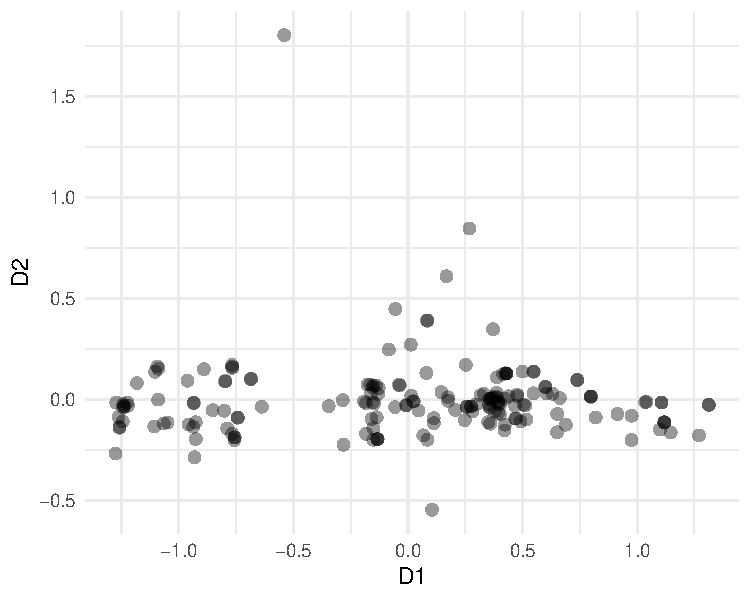
\includegraphics[width=\maxwidth]{figure/unnamed-chunk-3-1} 

}

\caption[MDS - Representación en $R^2$ de $D$]{MDS - Representación en $R^2$ de $D$}\label{fig:unnamed-chunk-3}
\end{figure}


\end{knitrout}

\label{fig:puntosD}



\subsection{Elección del Algoritmo de Agrupamiento}

A partir de la matriz de distancias $D$, y aplicando el tanto el algoritmo de agrupamiento CLARA como PAM, por ejemplo para formar $K=3$ grupos, se obtienen agrupaciones parecidas, tal como se puede ver en la figura \ref{fig:pam} , \ref{fig:clara}. Las ligeras semejanzas en los grupos formados obedece a que el algoritmo CLARA, usa el algoritmo PAM pero con remuestreo. Sin embargo, la diferencia radica en la velocidad de ejecución de ambos algoritmos, como ya lo se mencionaron en el capítulo anterior, el algoritmo CLARA es mucho más eficiente en la formación de grupos (considerando el tiempo de ejecución).



\begin{figure}[H]
\centering
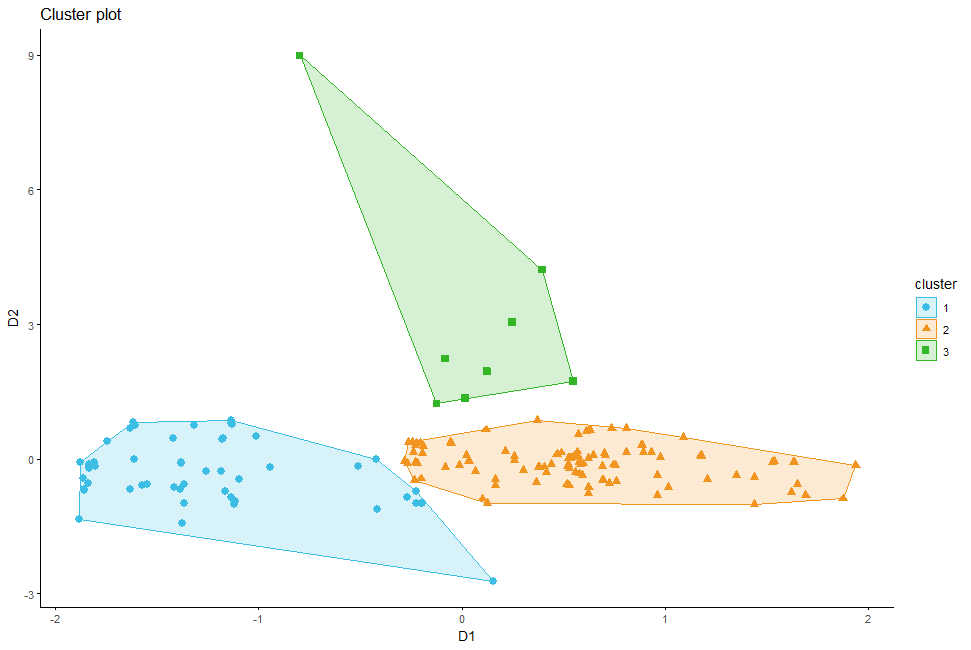
\includegraphics[scale=0.45]{Resultados/1_Pamk3}
\caption{Clústers generados con PAM}\label{fig:pam}
\end{figure}


\begin{figure}[H]
\centering
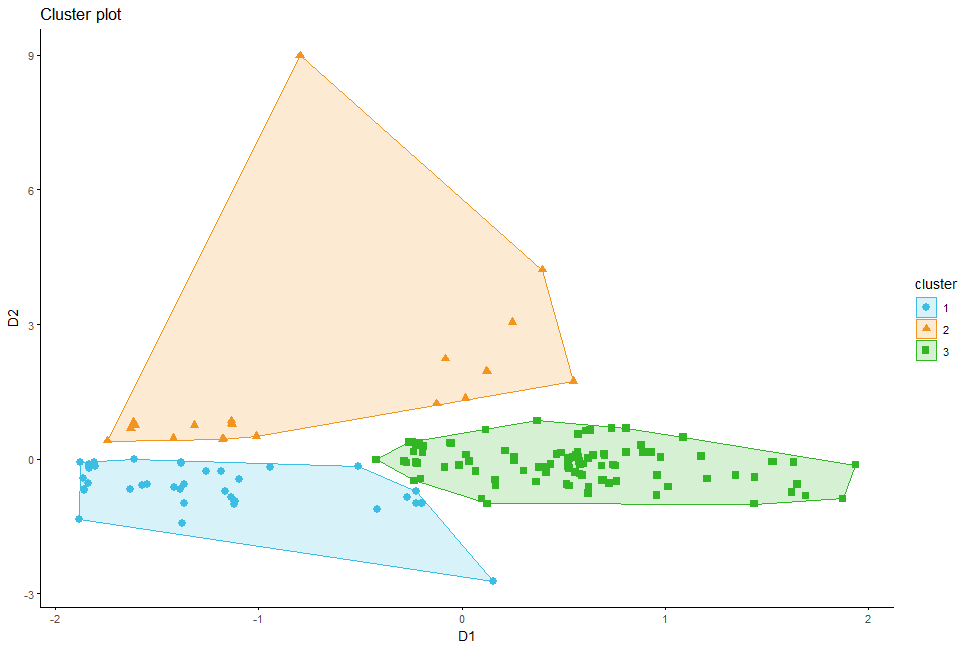
\includegraphics[scale=0.45]{Resultados/1_Clarak3}
\caption{Clústers generados con CLARA }\label{fig:clara}
\end{figure}




\subsection{Elección de número de clústers}
En esta sección, se hace uso del estadístico GAP, antes descrito, que permitirá hallar el número más adecuado de grupos, que hay que formar. Se resumen los resultados de este estadístico, para distintos número de clústers formados con el algoritmo CLARA, en la figura \ref{fig:k_opt}.

\begin{figure}[H]
\centering
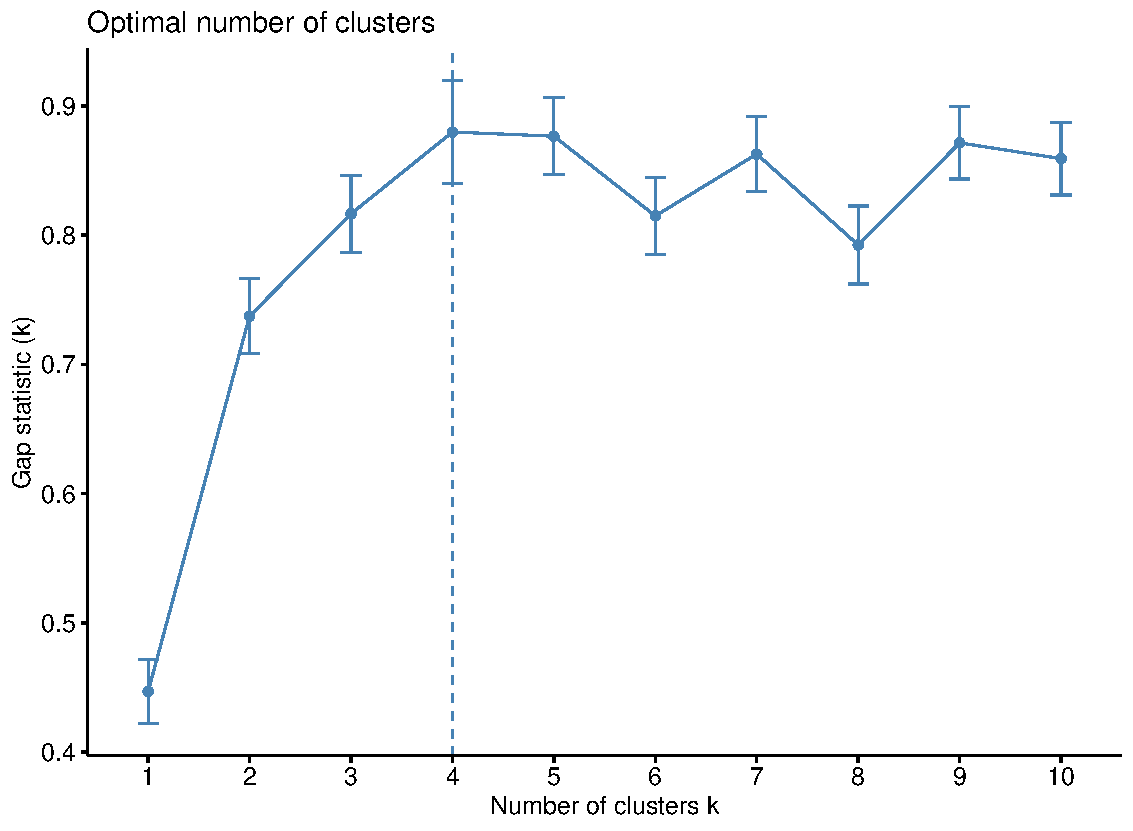
\includegraphics[scale=0.65]{Resultados/4_k_optimo_clusters}
\caption{Número Óptimo de Clusters }\label{fig:k_opt}
\end{figure}

Como se puede observar, el número óptimo de clústers en los que se debe agrupar las series de tiempo es $K=4$.


\subsection{Características de Clústers formados}
Elegido el número de clústers adecuado, se ejecuta el algoritmo CLARA con $K=4$ número de clústers, y se obtienen los distintos grupos a los que corresponde cada serie. A continuación, se analizarán distintas representaciones de los clústers.

\begin{enumerate}

%%%%%%%%%%%%%%%%%%%%%%%%%%%%%%
\item \textit{Representación en $\R^2$.} Como se puede apreciar en la figura \ref{fig:puntosR2}, las envolventes convexas de los puntos de cada clúster forman grupos bien definidos de puntos (estaciones), que a pesar de estar bastante cercanos, ninguno de ellos se sobrepone a los otros.

\begin{figure}[H]
\centering
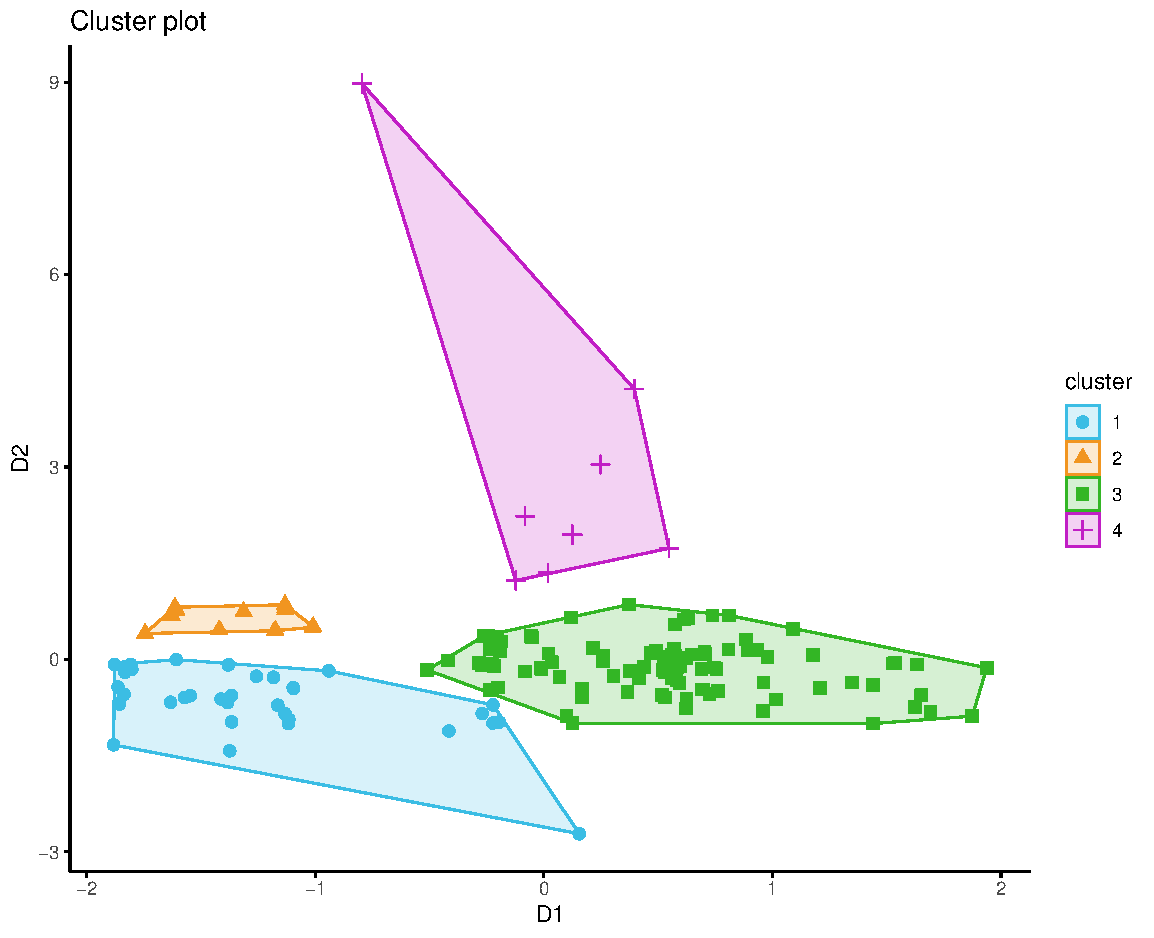
\includegraphics[scale=0.65]{Resultados/2_plot_cluster_dimensiones}
\caption{Representación de Clústers en $\R^2$ }\label{fig:puntosR2}
\end{figure}




%%%%%%%%%%%%%%%%%%%%%%%%%%%%%%
\item \textit{Representación geográfica.} Como se puede apreciar en la figura \ref{fig:mapa}, se observa que a diferencia de la representación de las estaciones en $\R^2$, no se tienen regiones bien definidas, hay clústers que poseen estaciones (de otros clústers) dentro de la región que delimitan sus elementos, por lo que parecerían mezclarse. Cabe la pena destacar que, viendo con mayor detalle, las serie de un mismo clúster tienden a disponerse sobre la ribera de un mismo río, como se ve por ejemplo en la figura \ref{fig:mapa_zoom}, esto se explicaría por la elección de la métrica con la que se construyeron los clústers, ya que considera la estructura temporal del caudal (medido en las estaciones) y deja de lado la escala. Así si en dos estaciones los caudales crecen (o decrecen) en espacios de tiempo parecidos, y si considerar a que escala, entonces su distancia $d_{ACF}$ será pequeña.


\begin{figure}[H]
\centering
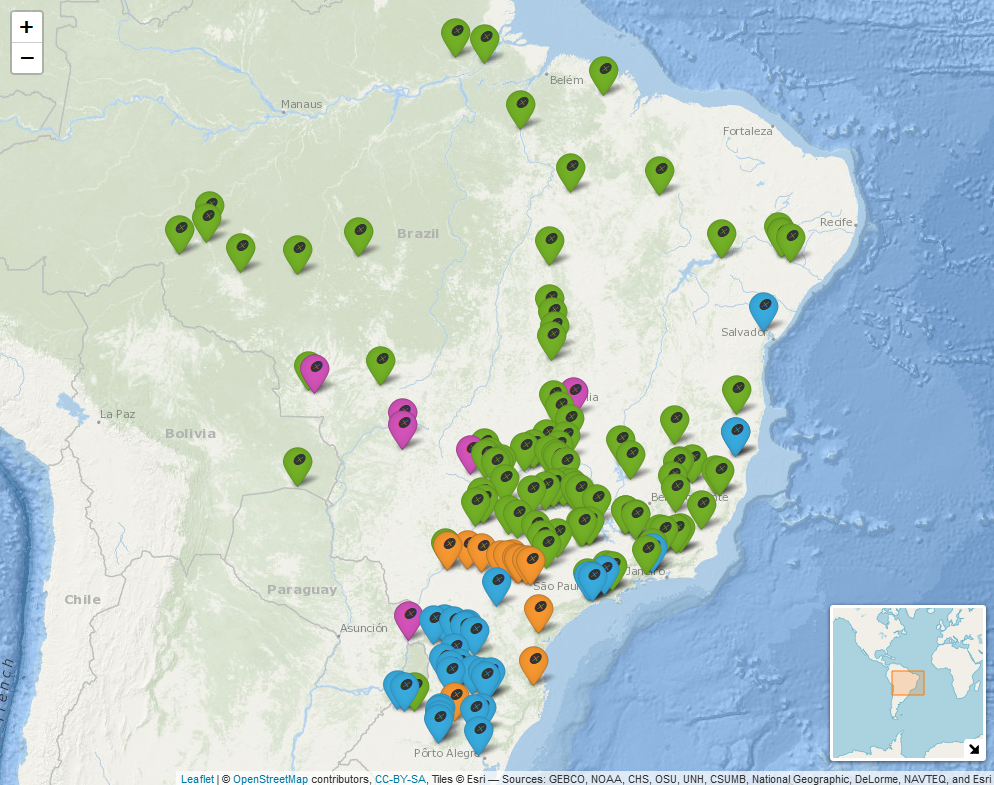
\includegraphics[scale=0.45]{Resultados/3_mapa_clusters}
\caption{Representación Geográfica de Clústers}\label{fig:mapa}
\end{figure}


\begin{figure}[H]
\centering
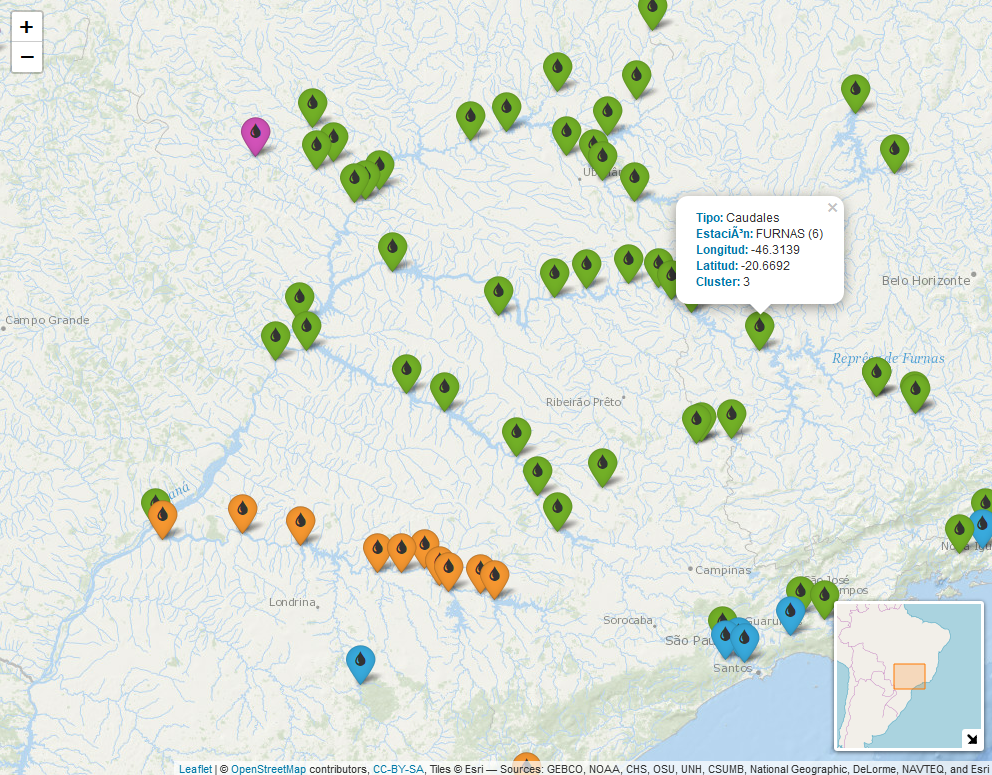
\includegraphics[scale=0.55]{Resultados/3_mapa_zoom}
\caption{Acercamiento a Clúster (representación Geográfica)}\label{fig:mapa_zoom}
\end{figure}



%%%%%%%%%%%%%%%%%%%%%%%%%%%%%%
\item \textit{Gráfico de las Series de Tiempo.} Como se puede observar en la figura \ref{fig:serie_clust1.1}, y como era de esperarse, las series de tiempo del Clúser 1, tiene un comportamiento parecido en todo el periodo considerado, variando solo en escala. Lo propio sucede en el Clúster 2 y 4, como se pude observar en las figuras \ref{fig:serie_clust1.2}, \ref{fig:serie_clust1.4}. Mientras que el Clúster 3 se observan series que parecen tener un comportamiento temporal menos parecido que el visto en los otros clústers, aunque tras una observación más minuciosa se observa que en realidad las series son parecidas considerando unos retardos.
% Resultados/Cluster 1/1_series_cluster.png
\begin{figure}[H]
\centering
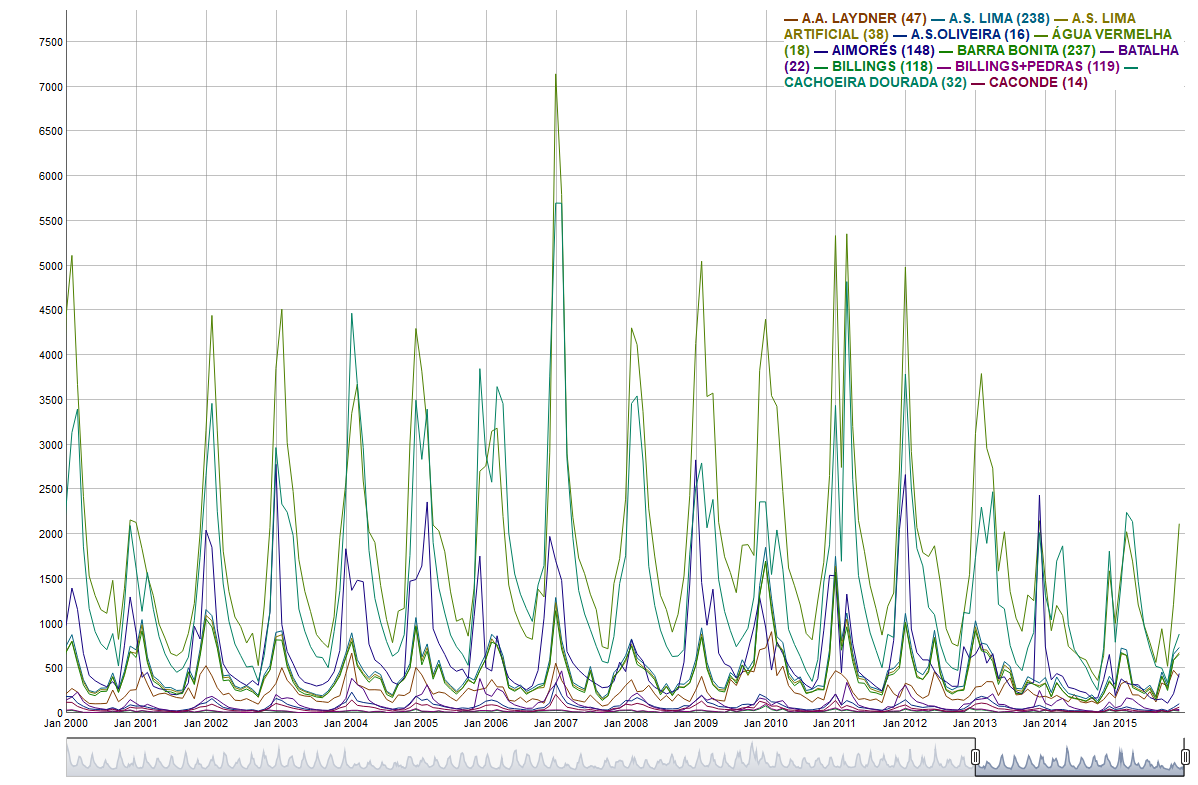
\includegraphics[scale=0.4]{Resultados/Cluster1/1_series_cluster}
\caption{Series de Tiempo del Clúster 1}\label{fig:serie_clust1.1}
\end{figure}


\begin{figure}[H]
\centering
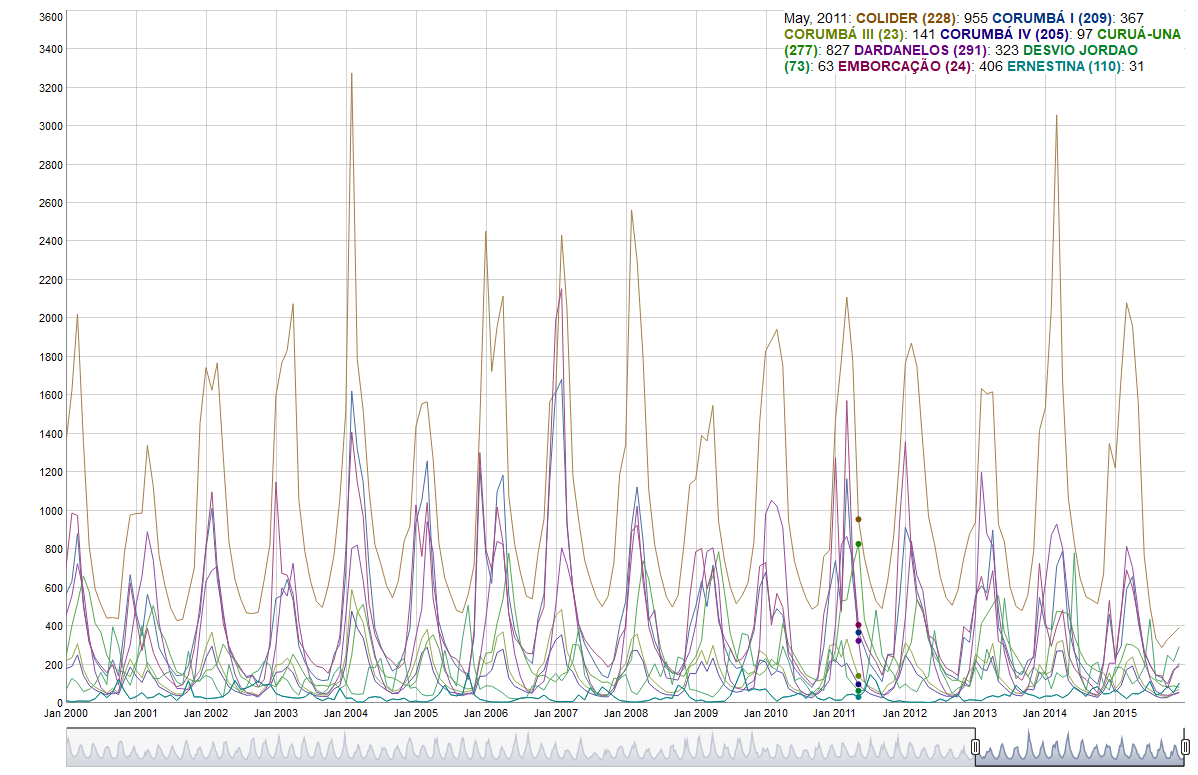
\includegraphics[scale=0.5]{Resultados/Cluster2/1_series_cluster}
\caption{Series de Tiempo del Clúster 2}\label{fig:serie_clust1.2}
\end{figure}

\begin{figure}[H]
\centering
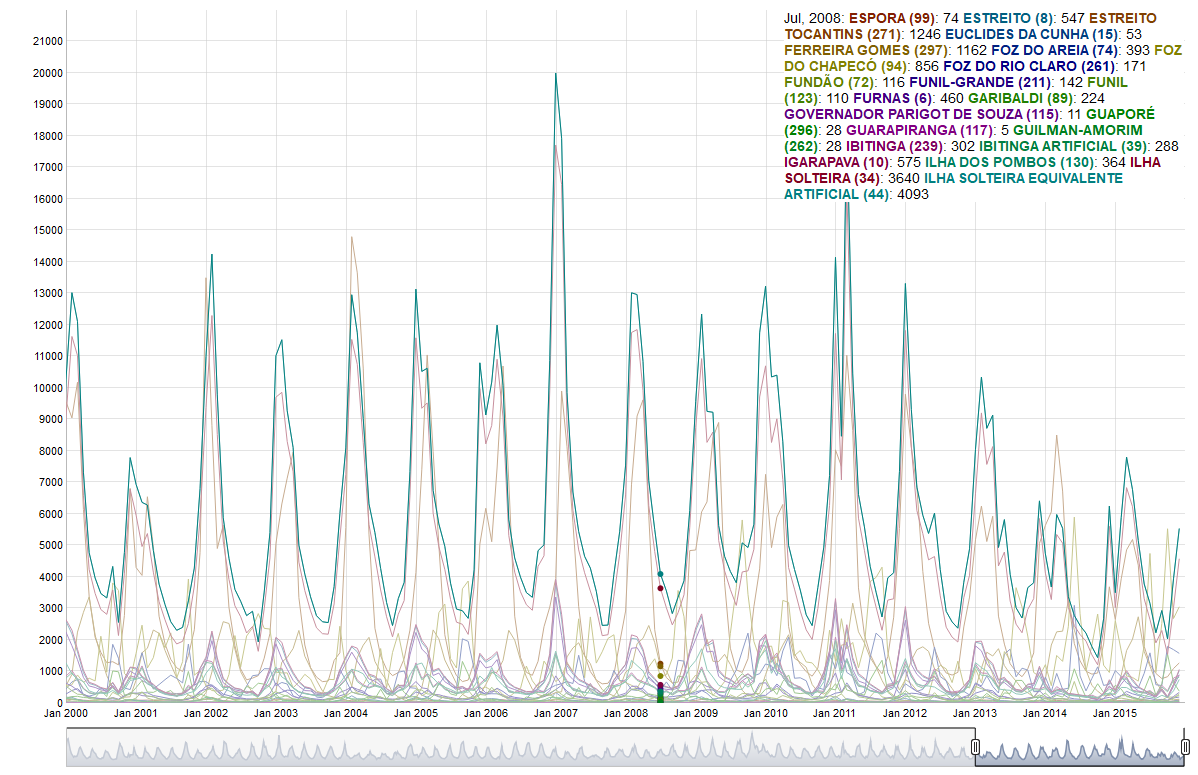
\includegraphics[scale=0.5]{Resultados/Cluster3/1_series_cluster}
\caption{Series de Tiempo del Clúster 3}\label{fig:serie_clust1.3}
\end{figure}

\begin{figure}[H]
\centering
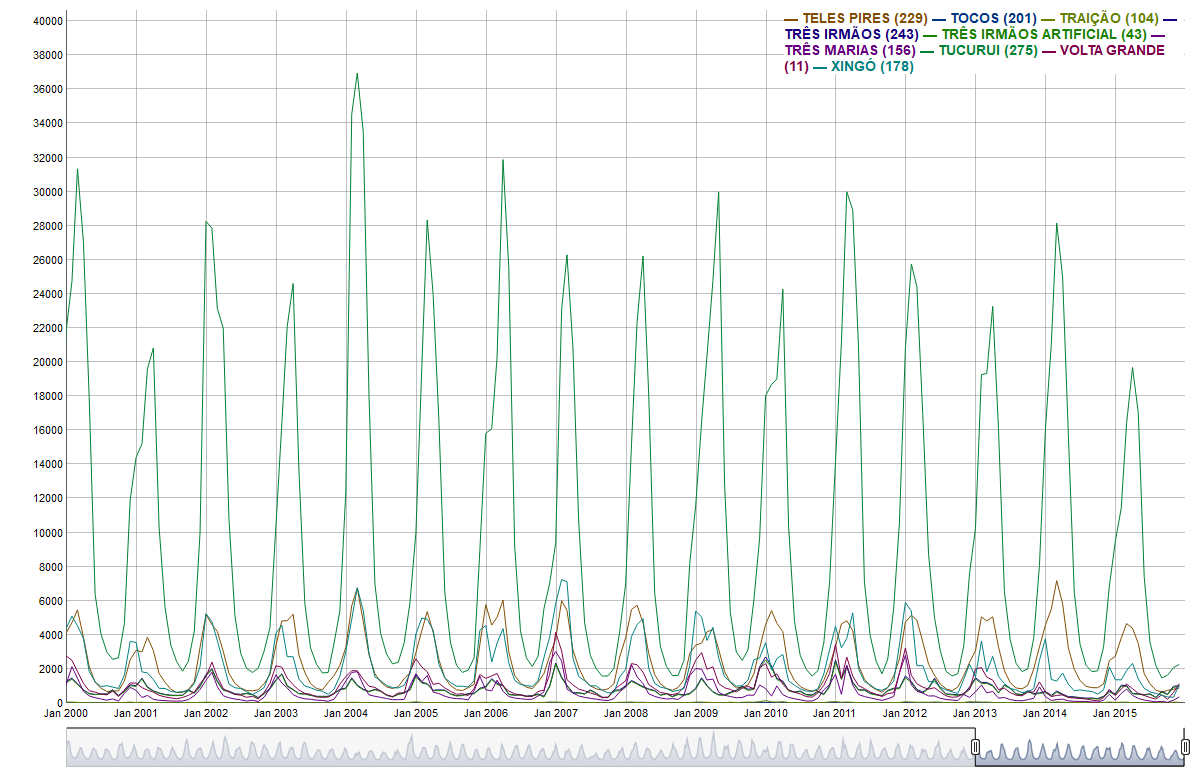
\includegraphics[scale=0.5]{Resultados/Cluster4/1_series_cluster}
\caption{Series de Tiempo del Clúster 4}\label{fig:serie_clust1.4}
\end{figure}





\end{enumerate}






%----------------------------------------------------------------------

% 
% \begin{figure}[h]
% \caption{Mapa de Clústers}
% 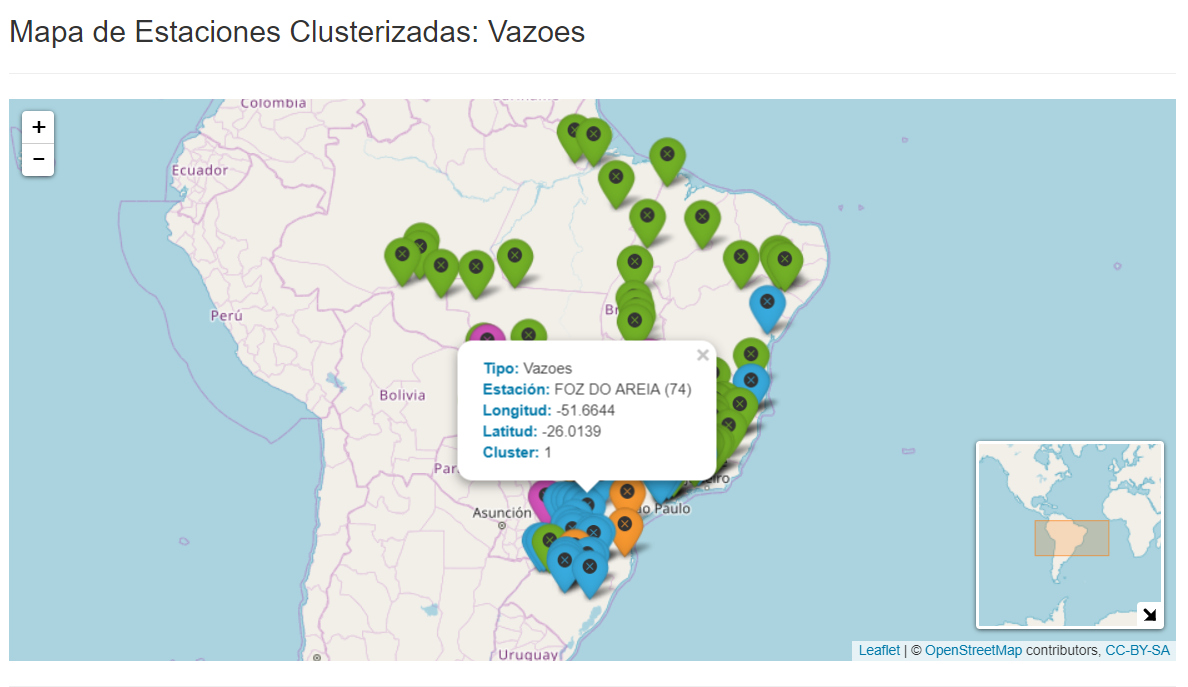
\includegraphics[width=15cm]{Cap3-Metodologia/Capture1.png}
% \label{fig:mapa_clust}
% \centering
% \end{figure}
% 
% 
% \begin{figure}[h]
% \caption{Series del Clúster 1}
% 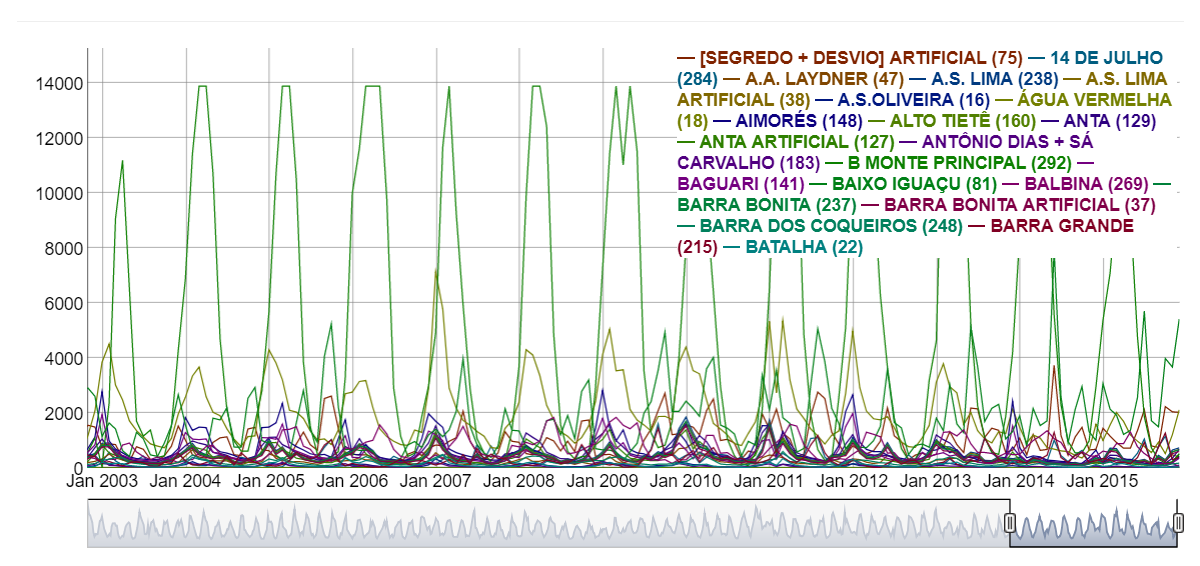
\includegraphics[width=15cm]{Cap3-Metodologia/Capture2.png}
% \label{fig:clust1}
% \centering
% \end{figure}

% \section{Análisis de Componente Principales Funcional}
% 
% El ACP típico se encarga de reducir la dimensión de un conjunto de datos mediante el cálculo de un grupo mucho menor de variables ortogonales que mejor representan el conjunto original de datos.
% Análogamente el análisis de componentes principales funcionales (ACPF) es una extensión del ACP clásico en el que las componentes principales están representadas por funciones y no por vectores, como lo detallamos en el capítulo anterior. 
% 
% Así, podemos usar todas las series de tiempo asociadas a los caudales de un clúster para hallar esta función (o funciones) que representan el comportamiento de todas las series del clúster. Esto bajo el supuesto de que todas las series de un clúster, son en realidad trayectorias de un mismo proceso estocástico. 
% 
% 
% \subsection{ACPF de los Clústers}
% En la figura \ref{fig:acp_summ1} podemos observar, en la esquina superior izquierda, un gráfico que muestra con cuantas observaciones se cuenta en cada punto de tiempo $t$, vemos que se cuenta con más de 4 observaciones, esto debido a que consideramos que cada serie del clúster conforma una observación del proceso. En la parte superior derecha podemos observar la función media del proceso, como vemos esta muestra un comportamiento estacional parecido al de las series que componen el clúster, por lo que más adelante la consideraremos como una candidata a ser representante del clúster, esto a pesar de que en un principio se planeaba usar una de las componentes principales con ese fin. En la parte inferior izquierda encontramos un gráfico que representa el porcentaje de variabilidad explicada por cada componente principal, como se puede observar la primera componente explica el $99\%$ de la variabilidad del proceso. Finalmente, el gráfico restante representa las 3 primeras componentes principales (funcionales), vemos que la primera de ellas es una curva suave casi constante, que no posee un comportamiento estacional, razón por la que se la descarta como posible serie representante del clúster.
% 
% \begin{figure}[H]
% 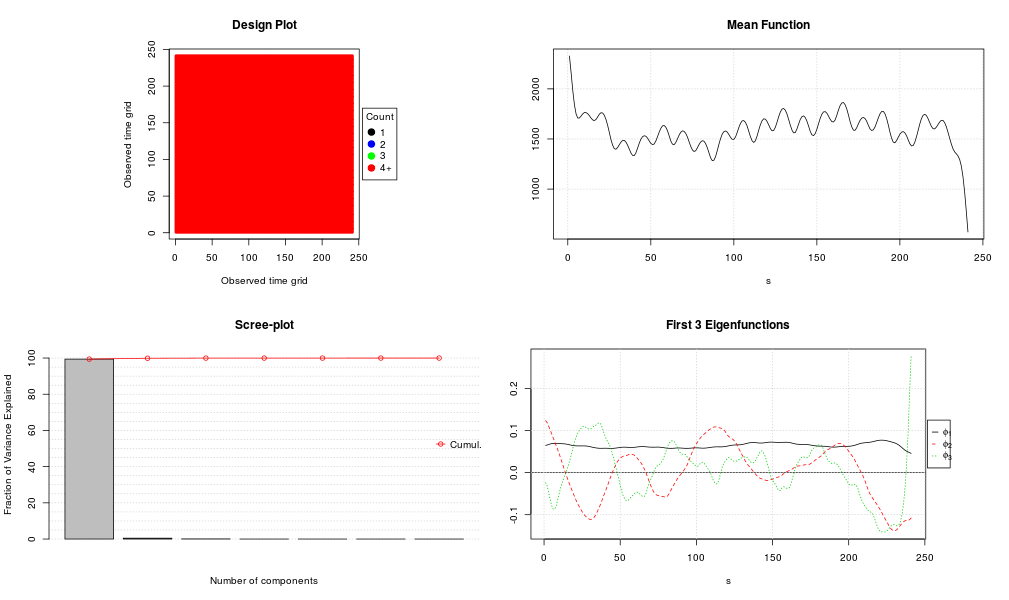
\includegraphics[width=15cm]{1_Cluster/ACPF}
% \caption{ACPF del Series del Clúster 1}
% \label{fig:acp_summ1}
% \centering
% \end{figure}
% 
% Otro gráfico interesante de analizar, es el de la covarianza, recordando que en el caso funcional la función de covarianza es una superficie. La covarianza estimada del proceso asociado al clúster 1 se ve en la parte izquierda de la figura \ref{fig:covar1}, como era de esperarse es una superficie con picos y valles, que indica el comportamiento estacional de todas las series que componen el clúster. 
% 
% \begin{figure}[H]
% 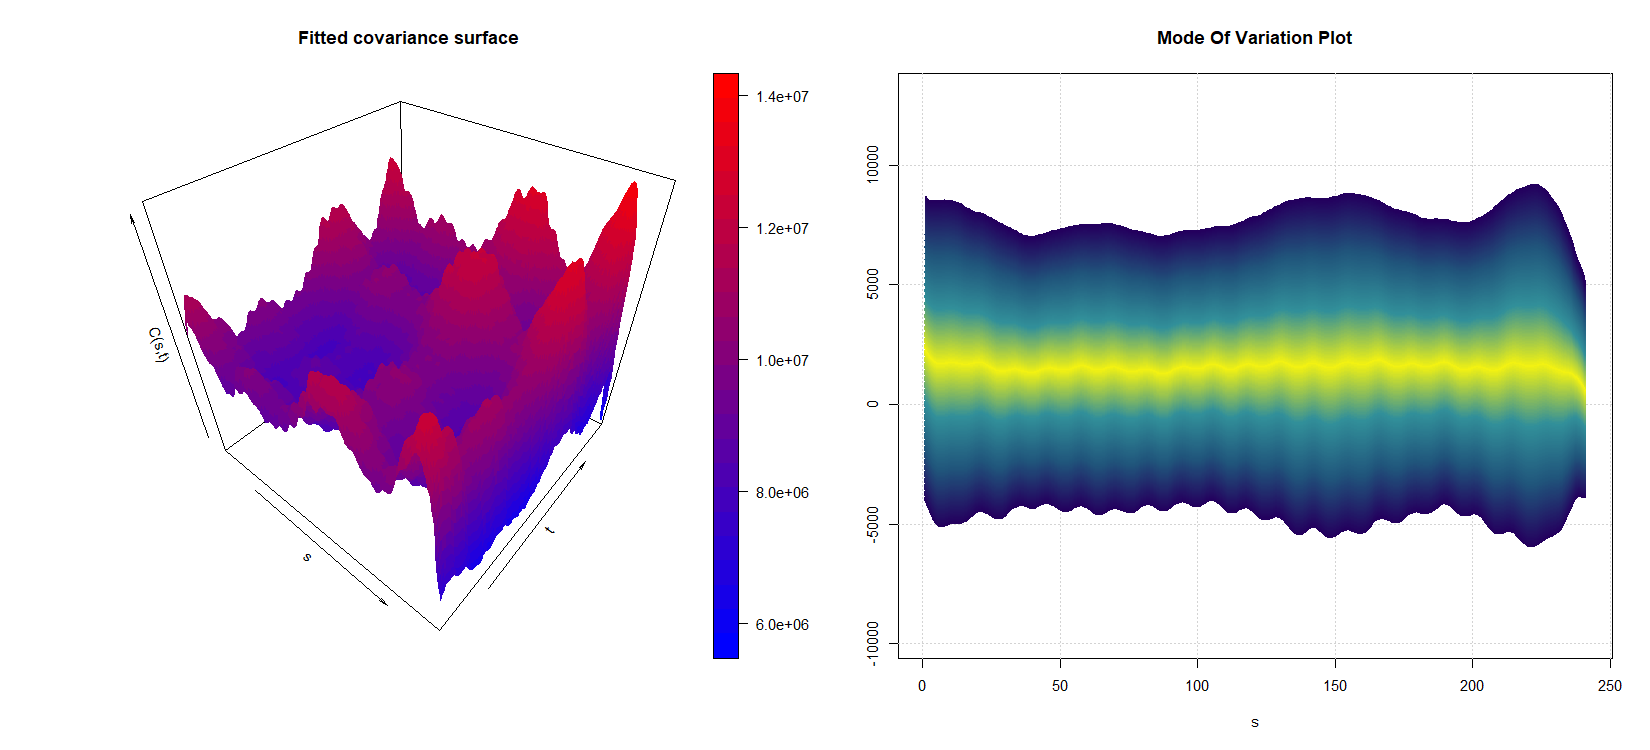
\includegraphics[width=15cm]{1_Cluster/covarianza}
% \caption{Superficie de Covarianza Estimada (Clúster 1)}
% \label{fig:covar1}
% \centering
% \end{figure}
% 
% En la parte derecha de la misma figura encontramos un gráfico de modos de variación, este gráfico se usa para identificar niveles inusuales de variación en un proceso que esta compuesto por varias réplicas (trayectorias), cerca de la franja amarilla vemos hallamos trayectorias (series) cuyo comportamiento es más usual, es decir, la mayoría de trayectorias sigue esa tendencia, mientras que hacía los extremos (en color azul oscuro) encontramos las trayectorias menos comunes. Podemos evidenciar de igual manera un comportamiento periódico que es otra evidencia más de la estacionalidad que poseen las series del clúster. 
% 
% \paragraph{Observación.} Las gráficas correspondientes a los otros tres clústers se encuentran en el apéndice \ref{ap:acpf}.
% 



%%%%%%%%%%%%%%%%%%%%%%%%%%%%%%%%%%%%%%%%%%%%%%%%%%%%%%%%%%%%%%%%%
%----------------------------------------------------------------
%%%%%%%%%%%%%%%%%%%%%%%%%%%%%%%%%%%%%%%%%%%%%%%%%%%%%%%%%%%%%%%%%

\section{Modelamiento de Series de tiempo}

En esta sección, se plantearán dos modelos para cada clúster. Por una parte, se plantea un modelo SARIMA aplicado a un representate del clúster, una primera idea era considerar la como serie representativa a la primera componente principal obtenida del ACP funcional del clúster, si embargo como se pudo constatar en la sección anterior, dicha serie no recoge el comportamiento estacional de los caudales, por esta razón se optó por elegir a la media funcional de las series (vistas como trayectorias de un mismo proceso estocástico), que como se vio tiene un comportamiento bastante similar, aunque suavizado, al de todas las series del clúster.

El segundo modelo que se plantea es un modelo SARIMAX aplicado a la serie \textit{medoide} del clúster, es decir, aquella serie más centralmente ubicada (en términos de la métrica $d_{ACF}$), estas series se obtienen durante la ejecución del algoritmo de agrupamiento CLARA (y también PAM). Considerando en este caso como variables regresoras a las series climáticas, de la estación geográficamente más cercana a la estación de medición de caudales.

A continuación, se muestra un paso previo, la limpieza de los datos que se poseen, necesaria para un correcto modelamiento de series temporales.

\paragraph{Limpieza de Datos de Clima} Un punto importante previo al modelamiento, es la limpieza de los datos. En este caso se cuenta con una alta presencia de valores perdidos especialmente en las series asociadas a variables Climáticas. Por lo que se decidió retirar todas aquellas series que contengan más del $10\%$ de valores perdidos. 
Mientras que para las restantes, se aplica el algoritmo de limpieza a los valores perdidos de las series climáticas  (\ref{sec:limpieza}). 

Pues bien, aplicando el algoritmo de de limpieza a las 4 variables climáticas (Precipitación, temperatura máxima, temperatura mínima, y humedad relativa), se obtuvieron valores simulados que concuerdan con los valores conocidos, considerando que las series, luego de este proceso de limpieza, no alteraron su estructura general, tal como se puede ver en la figura \ref{fig:climaLimp2}.



\begin{figure}[H]
\centering
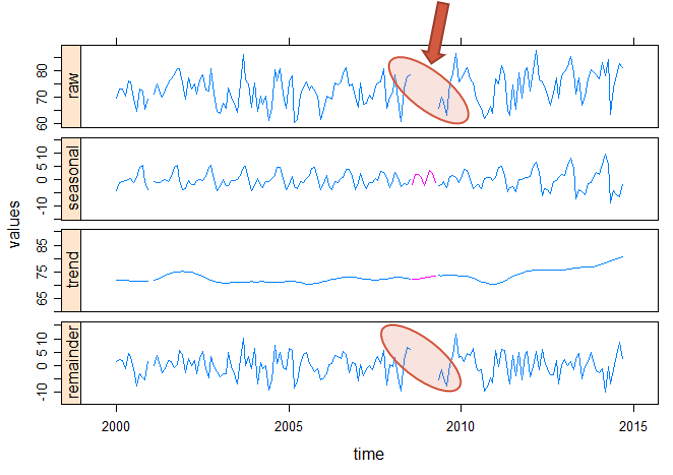
\includegraphics[width=10cm]{Cap3-Metodologia/limpieza.png}
\caption{Serie de Tiempo Climática}
\label{fig:clima2}

\end{figure}


\begin{figure}[H]
\centering
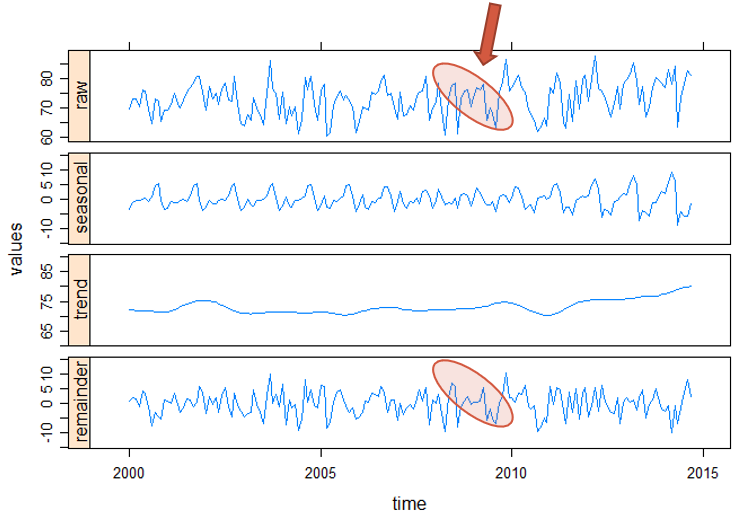
\includegraphics[width=10cm]{Cap3-Metodologia/limpieza2.png}
\caption{Serie de Tiempo Climática Corregida}
\label{fig:climaLimp2}

\end{figure}

%%%%%%%%%%%%%%%%%%%%%%%%%%%%%%%%%%%%%%%%%%%%%%%%%%%%%%%%%%%%%%

% \section{Agrupar datos de Caudales y Clima}
% 
% Una vez corregidas las series climáticas, el criterio para agrupar las series climáticas con series de caudales de determinado clúster es el siguiente:  Para cada serie de Caudales del clúster se busca la serie climática de la estación más cercana, 
% 
% Finalmete esta lista de estaciones climáticas (y las 4 variables que la conforman) constituyen las variables explicativas del modelo que plantearemos adelante para poder explicar el comportamiento del Caudal de cada Clúster, es decir, de la serie de Caudales que representa el clúster obtenida del ACP-Funcional.
% 
% \begin{figure}[h]
% \caption{Serie de Tiempo Climática Corregida}
% 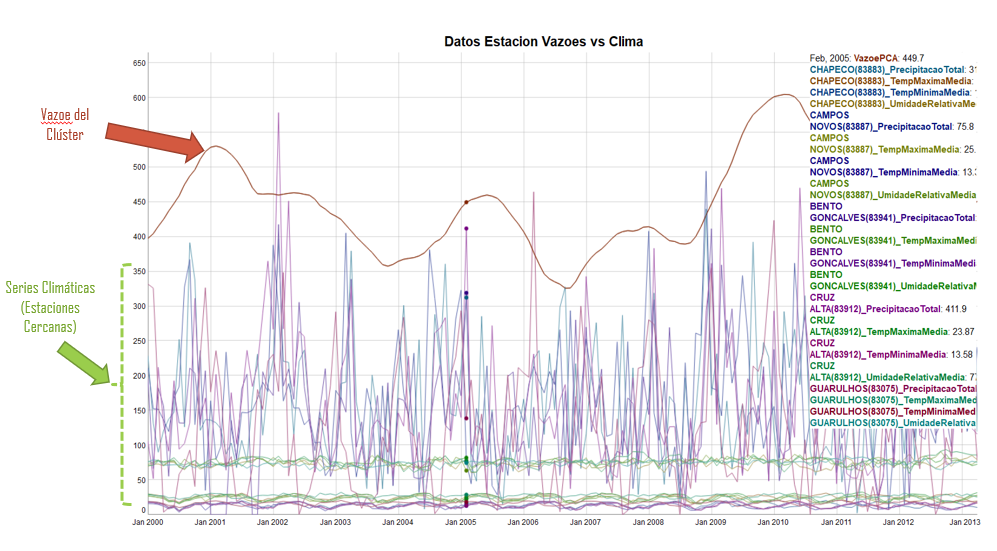
\includegraphics[width=16cm]{Cap3-Metodologia/vazclim.png}
% \label{fig:acpf1}
% \centering
% \end{figure}

%%%%%%%%%%%%%%%%%%%%%%%%%%%%%%%%%%%%%%%%%%%%%%%%%%%%%%%%%%%%%%%%%

\subsection{Modelo SARIMA del Clúster}

Como se mencionó anteriormente, se modelará una serie representante del clúster, en este caso la media funcional de las series de caudales que lo componen (ver figura \ref{fig:sarima_serie}), para ello se sigue la metodología Box y Jenkins, por lo que se analizará en primer lugar la función de Autocorrelación y Autocorrelación Parcial de la serie, como se puede ver en la figura \ref{fig:sarima_acf}, se tienen picos fuera de las bandas de confianza, que se repiten periódicamente (cada 12 retardos). 




%  Corregir con graficos R



% \begin{figure}[h]
% \centering
% 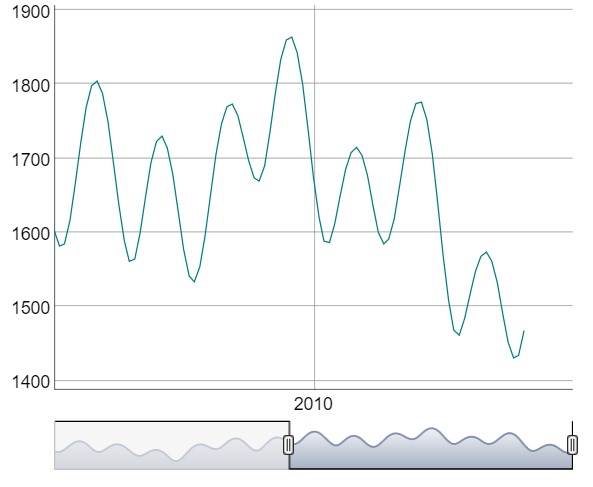
\includegraphics[width=13cm]{1_Cluster/sarima_serie}
% \caption{Media Funcional (Clúster 1)}
% \label{fig:sarima_serie}
% 
% \end{figure}


% \begin{figure}[H]
% \centering
% 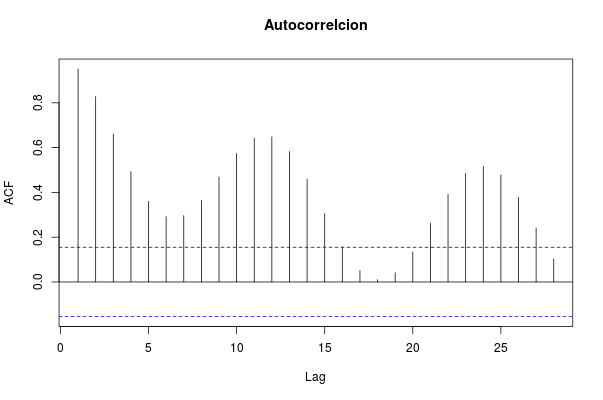
\includegraphics[width=13cm]{1_Cluster/sarima_autocorr1}
% \caption{Función de Autocorrelación: Media Funcional (Clúster 1)}
% \label{fig:sarima_acf}
% 
% \end{figure}
% 
% \begin{figure}[H]
% \centering
% 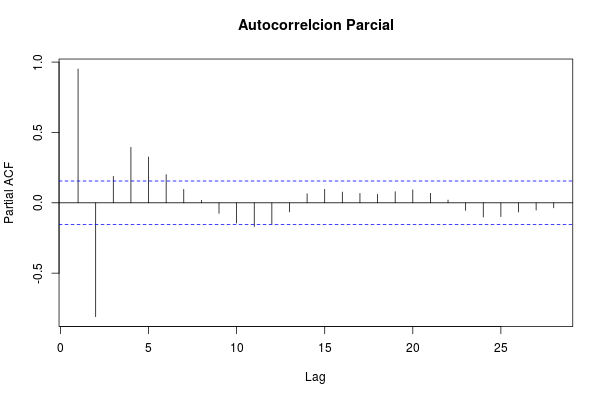
\includegraphics[width=13cm]{1_Cluster/sarima_autocorrP1}
% \caption{Función de Autocorrelación: Media Funcional (Clúster 1)}
% \label{fig:sarima_pacf}
% 
% \end{figure}











\begin{knitrout}
\definecolor{shadecolor}{rgb}{0.969, 0.969, 0.969}\color{fgcolor}\begin{figure}[H]

{\centering 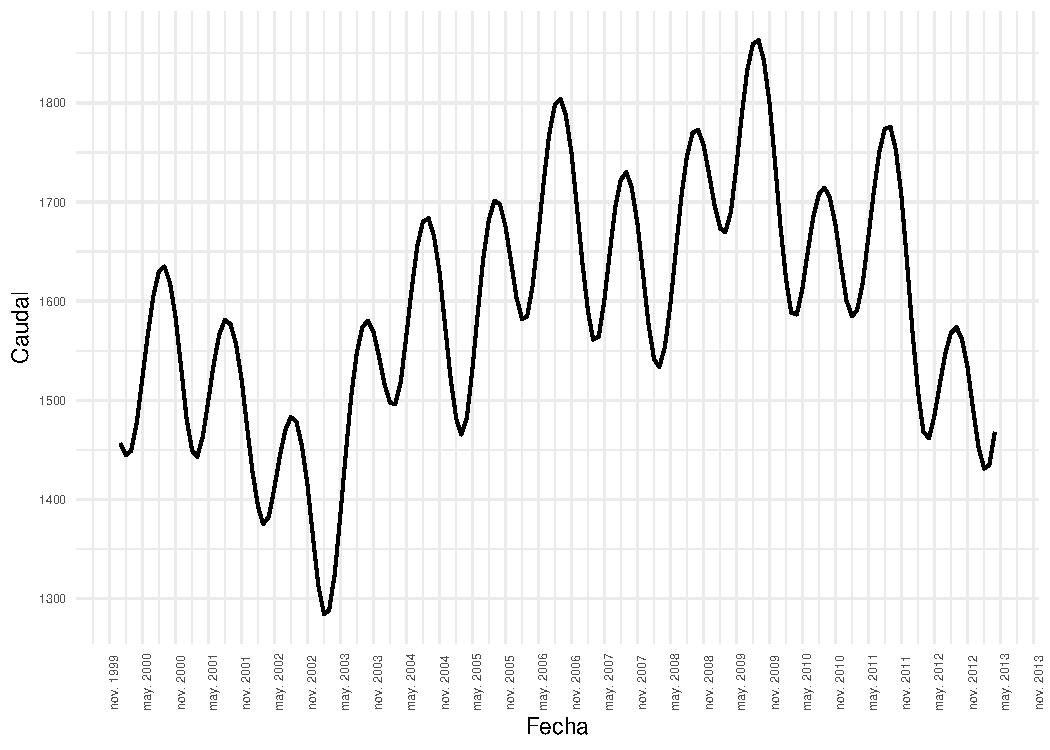
\includegraphics[width=\maxwidth]{figure/unnamed-chunk-7-1} 

}

\caption{\label{fig:sarima_serie} Caudal - Clúster 1}\label{fig:unnamed-chunk-7}
\end{figure}


\end{knitrout}



\begin{knitrout}
\definecolor{shadecolor}{rgb}{0.969, 0.969, 0.969}\color{fgcolor}\begin{figure}[H]

{\centering 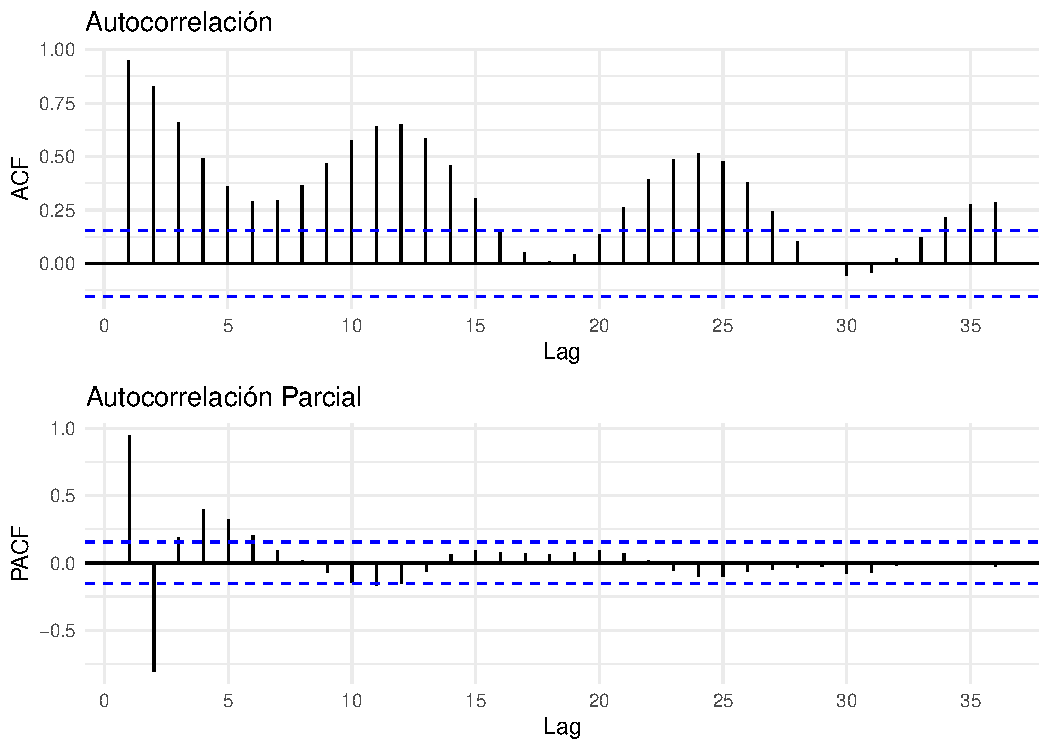
\includegraphics[width=\maxwidth]{figure/unnamed-chunk-8-1} 

}

\caption{\label{fig:sarima_acf} Función de Autocorrelación Caudal - Clúster 1}\label{fig:unnamed-chunk-8}
\end{figure}


\end{knitrout}







Es evidente que esta serie no es estacionaria, y que es necesaria una diferenciación de tipo estacional (ver figura \ref{fig:sarima_seried1}). Después de diferencial estacionalmente, se tiene una función de autocorrelación que no decrece rápidamente y que en varios retardos se encuentra fuera de las bandas de confianza (ver figura \ref{fig:sarima_acf2}). Aunque se puede aplicar el test de Dickey Fuller para ver si es necesaria una diferenciación (no estacional) adicional.
% Test de DICKEY FULLER


\begin{knitrout}
\definecolor{shadecolor}{rgb}{0.969, 0.969, 0.969}\color{fgcolor}\begin{kframe}
\begin{verbatim}
## 
## 	Augmented Dickey-Fuller Test
## 
## data:  vazd1
## Dickey-Fuller = -3.8929, Lag order = 5, p-value = 0.01643
## alternative hypothesis: stationary
\end{verbatim}
\end{kframe}
\end{knitrout}
\label{tab:dfuller}





\begin{knitrout}
\definecolor{shadecolor}{rgb}{0.969, 0.969, 0.969}\color{fgcolor}\begin{figure}[H]

{\centering 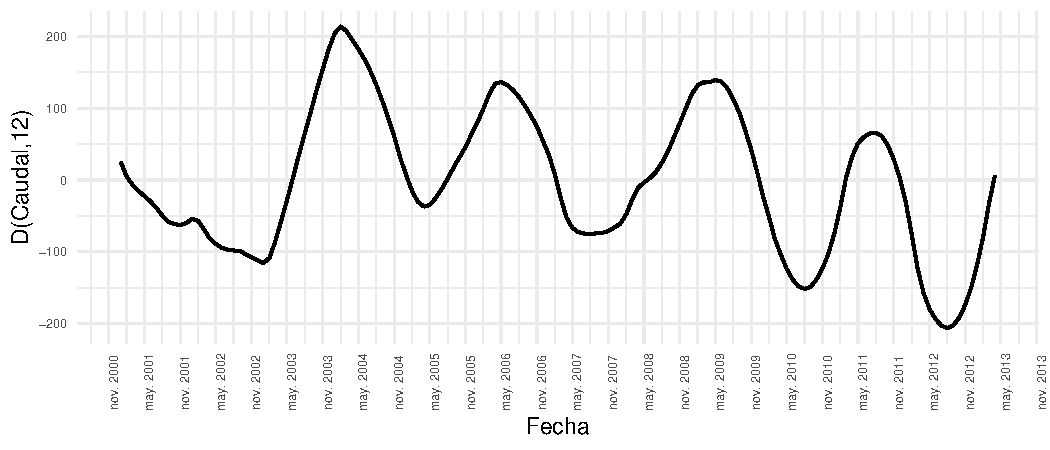
\includegraphics[width=\maxwidth]{figure/unnamed-chunk-10-1} 

}

\caption{\label{fig:sarima_seried1} D(Caudal,12) - Clúster 1}\label{fig:unnamed-chunk-10}
\end{figure}


\end{knitrout}



\begin{knitrout}
\definecolor{shadecolor}{rgb}{0.969, 0.969, 0.969}\color{fgcolor}\begin{figure}[H]

{\centering 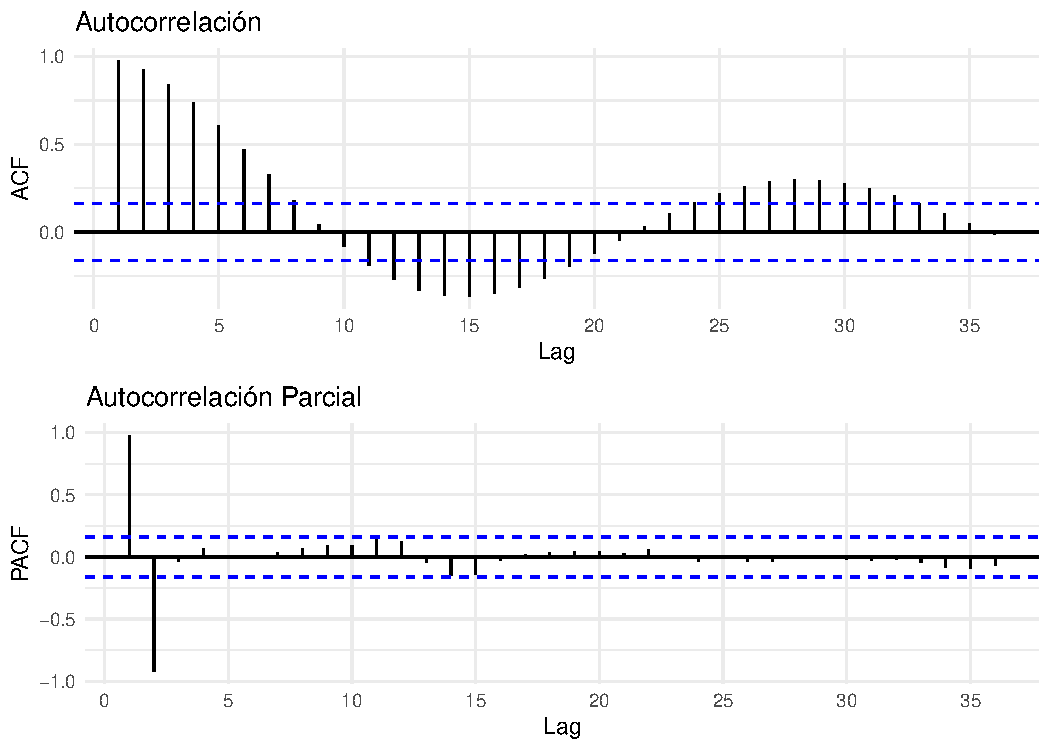
\includegraphics[width=\maxwidth]{figure/unnamed-chunk-11-1} 

}

\caption{\label{fig:sarima_acf2} Función de Autocorrelación D(Caudal,12) - Clúster 1}\label{fig:unnamed-chunk-11}
\end{figure}


\end{knitrout}



%%%%%%%%%%%  Funcion crear tablas modelos 








%%%%%%%%%%%%%%%%%%%%%%%%%%%%%%%%%

%  Tabla resumen Modelo 1



% \newpage
Como se puede ver en \ref{tab:dfuller}, el test de Dickey Fuller arroja un $\text{P-valor} = 0.016 < 0.05$, por lo que se concluye que el proceso ya es estacionario. Pues bien, en este punto se conocen los parámetros $d=0$ y $D=1$ del modelo SARIMA, resta identificar los órdenes $p, P, q$ y $Q$ de los polinomios Autoregresivos y Medias Móviles. Para ello, nótese que la función de autocorrelación parcial posee picos fuera de las  bandas hasta el retardo 5, por lo que la parte autoregresiva del modelo podría incluir 5 retardos, por lo tanto, se empieza planteando un modelo SARIMA$(5,0,0)(0,1,0)_{12}$. 

\begin{knitrout}
\definecolor{shadecolor}{rgb}{0.969, 0.969, 0.969}\color{fgcolor}\begin{table}

\caption{\label{tab:unnamed-chunk-14}\label{mod:sarima1}Modelo SARIMA$(5,0,0)(0,1,0)_{12}$}
\centering
\begin{threeparttable}
\begin{tabular}[t]{lrrrrl}
\toprule
Coef & Estimate & Std.Error & z-value & Pr(>|z|) & Signif\\
\midrule
\rowcolor{gray!6}  ar1 & 2.6400 & 0.0839 & 31.4736 & 0.0000 & ***\\
ar2 & -2.6453 & 0.2363 & -11.1939 & 0.0000 & ***\\
\rowcolor{gray!6}  ar3 & 1.2955 & 0.3064 & 4.2280 & 0.0000 & ***\\
ar4 & -0.3321 & 0.2367 & -1.4028 & 0.1607 & \\
\rowcolor{gray!6}  ar5 & 0.0215 & 0.0846 & 0.2548 & 0.7989 & \\
\bottomrule
\end{tabular}
\begin{tablenotes}
\item \textit{Resumen:} 
\item sigma\textasciicircum{}2 = 12.49, loglikelihood = -402.23, AIC = 816.45, BIC =834.43, Hannan-Quinn =824.72
\end{tablenotes}
\end{threeparttable}
\end{table}


\end{knitrout}


Como se puede ver en la tabla \ref{mod:sarima1}, los coeficientes asociados a los dos mayores retardos del polinomio AR son no significativos, por lo que es posible que sea necesario quitarlos del modelo. Por otra parte analizando los residuos del modelo, se puede observar por una parte que la función de Autocorrelación se encuentra dentro de las bandas de confianza, excepto en el retardo 12, por otro lado analizando los P-valores del Test Portmanteau (ver figura \ref{fig:sarima_residJ1}), en la versión de Ljung-Box, se observa que estos son menores a 0.05 a partir del retardo 7, por lo que se concluye que los residuos son significativos. Por lo tanto, no se rechaza la independencia de los residuos de este modelo, así que es necesario modificarlo.



% \label{fig:sarima_resid1}


\begin{knitrout}
\definecolor{shadecolor}{rgb}{0.969, 0.969, 0.969}\color{fgcolor}\begin{figure}[H]

{\centering 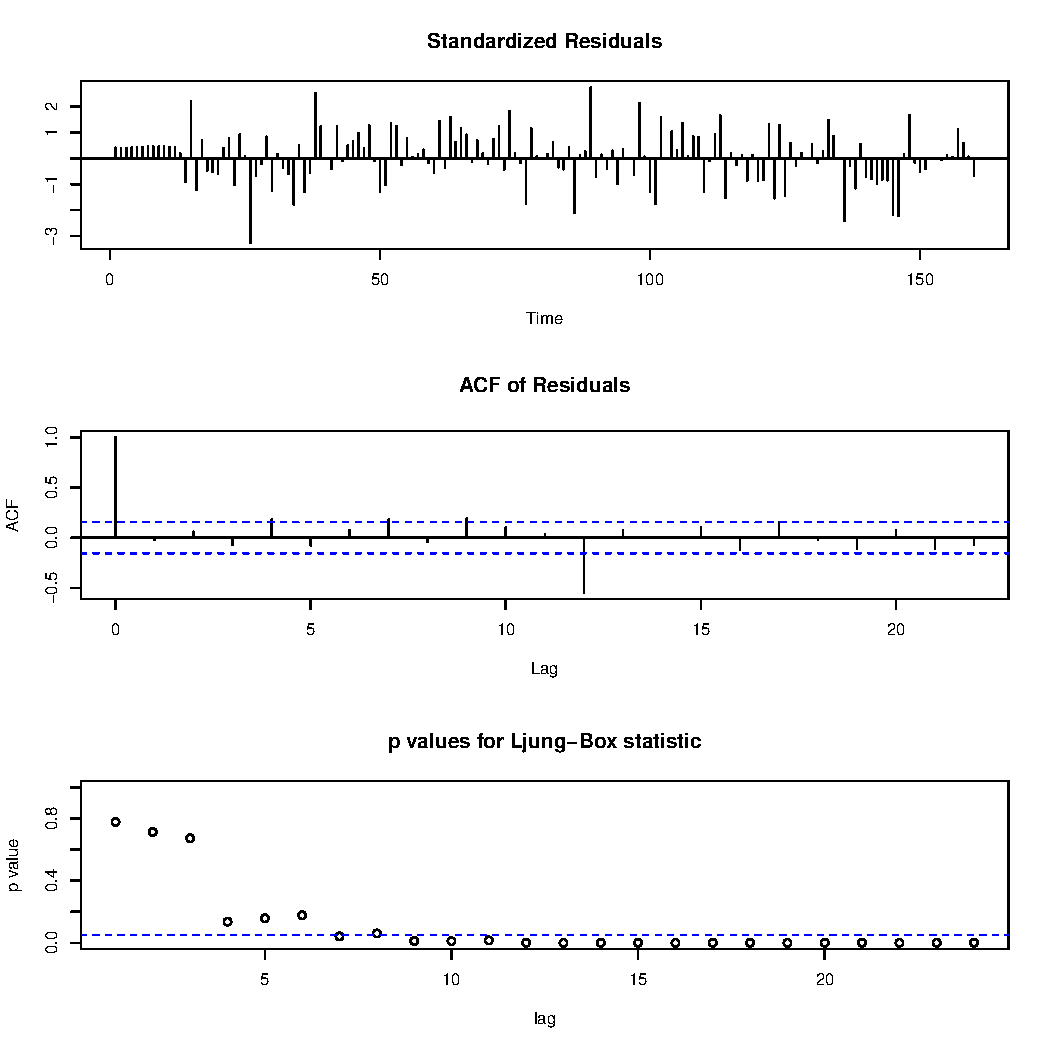
\includegraphics[width=\maxwidth]{figure/unnamed-chunk-15-1} 

}

\caption{\label{fig:sarima_residJ1} Residuos - Test Portmanteau (Ljung-Box) SARIMA(5,0,0)(0,1,0)}\label{fig:unnamed-chunk-15}
\end{figure}


\end{knitrout}

% \label{fig:sarima_residJ1}


Considerando ahora un orden menor del polinomio autoregresivo, debido a que los coeficiente asociados a los mayores retardos resultaron no ser significativos. Tras probar con el modelo SARIMA$(4,0,0)(0,1,0)_{12}$, se puede ver que todos sus coeficientes son significativos (\ref{mod:sarima_resid12}).


\begin{knitrout}
\definecolor{shadecolor}{rgb}{0.969, 0.969, 0.969}\color{fgcolor}\begin{table}

\caption{\label{tab:unnamed-chunk-16}\label{mod:sarima_resid12}Modelo SARIMA(4,0,0)(0,1,0)_{12}}
\centering
\begin{threeparttable}
\begin{tabular}[t]{lrrrrl}
\toprule
Coef & Estimate & Std.Error & z-value & Pr(>|z|) & Signif\\
\midrule
\rowcolor{gray!6}  ar1 & 2.6340 & 0.0805 & 32.709 & 0e+00 & ***\\
ar2 & -2.6185 & 0.2117 & -12.367 & 0e+00 & ***\\
\rowcolor{gray!6}  ar3 & 1.2392 & 0.2124 & 5.835 & 0e+00 & ***\\
ar4 & -0.2754 & 0.0814 & -3.383 & 7e-04 & ***\\
\bottomrule
\end{tabular}
\begin{tablenotes}
\item \textit{Resumen:} 
\item sigma\textasciicircum{}2 = 12.49, loglikelihood = -402.26, AIC = 814.52, BIC =829.5, Hannan-Quinn =821.41
\end{tablenotes}
\end{threeparttable}
\end{table}


\end{knitrout}


En cuanto a los residuos de este modelo se puede ver en la figura \ref{fig:sarima_resid12} que la función de autocorrelación tiene un pico fuera de las bandas únicamente en el retardo 12, por lo que es posible que sea necesario incorporar un retardo del polinomio media móvil (MA) o autoregresivo (AR) estacional. Además, se puede observar que los p-valores del estadístico de Ljung-Box aun son menores que 0.05 después del séptimo retardo.


\begin{knitrout}
\definecolor{shadecolor}{rgb}{0.969, 0.969, 0.969}\color{fgcolor}\begin{figure}[H]

{\centering 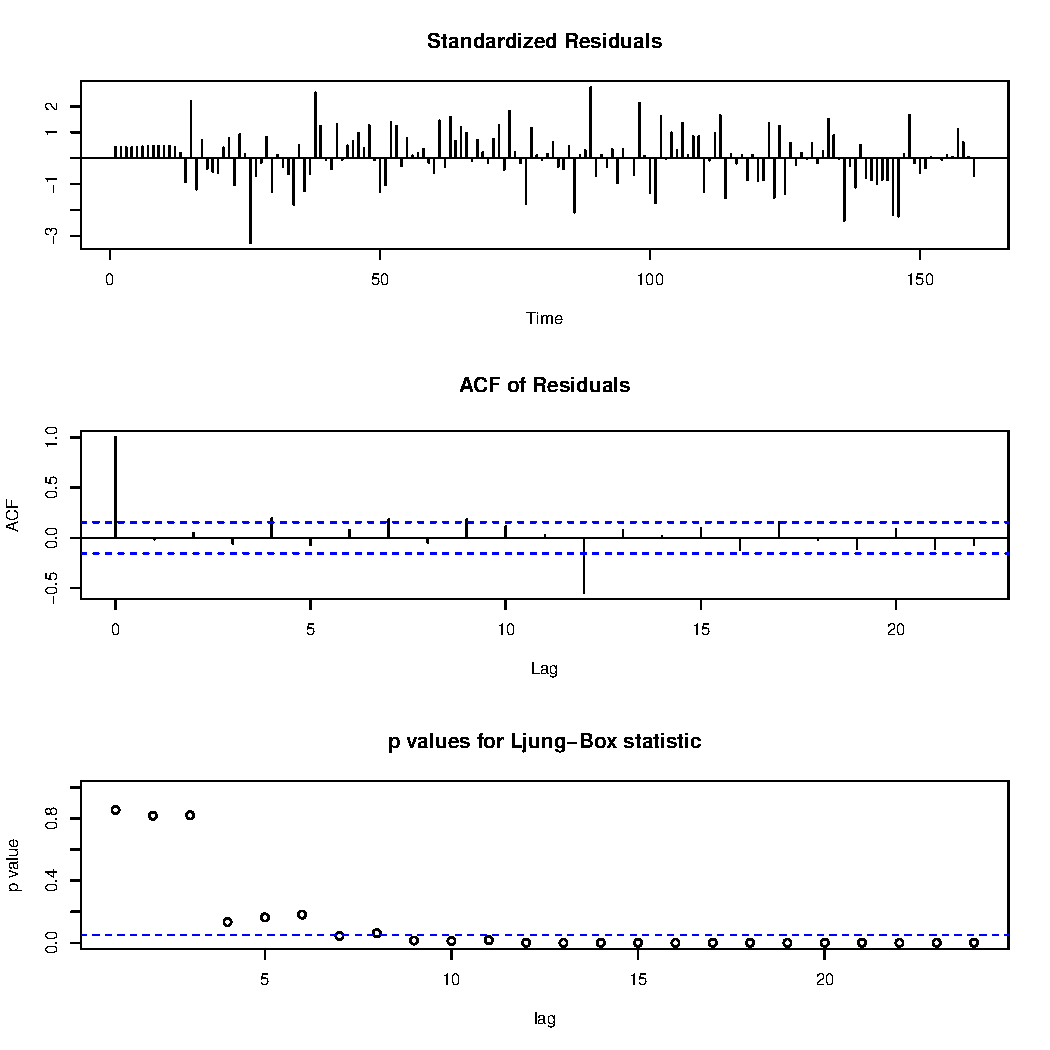
\includegraphics[width=\maxwidth]{figure/unnamed-chunk-17-1} 

}

\caption{\label{fig:sarima_resid12} Residuos - Test Portmanteau (Ljung-Box) SARIMA(4,0,0)(0,1,0)}\label{fig:unnamed-chunk-17}
\end{figure}


\end{knitrout}


Pues bien, agregando ahora al modelo el primer retardo del polinomio autoregresivo estacional, con lo que se plantearía un modelo SARIMA$(4,0,0)(1,1,0)_{12}$. Tal como se puede ver en la tabla \ref{mod:sarima_resid13}, se obtiene un modelo con todos los coeficientes significativos, y con residuos independientes, tal como se puede ver en la figura \ref{fig:sarima_resid13}. 

\begin{knitrout}
\definecolor{shadecolor}{rgb}{0.969, 0.969, 0.969}\color{fgcolor}\begin{table}

\caption{\label{tab:unnamed-chunk-18}\label{mod:sarima_resid13}Modelo SARIMA$(4,0,0)(1,1,0)_{12}$}
\centering
\begin{threeparttable}
\begin{tabular}[t]{lrrrrl}
\toprule
Coef & Estimate & Std.Error & z-value & Pr(>|z|) & Signif\\
\midrule
\rowcolor{gray!6}  ar1 & 2.6590 & 0.0806 & 32.970 & 0.0000 & ***\\
ar2 & -2.6100 & 0.2147 & -12.155 & 0.0000 & ***\\
\rowcolor{gray!6}  ar3 & 1.1814 & 0.2148 & 5.499 & 0.0000 & ***\\
ar4 & -0.2390 & 0.0810 & -2.950 & 0.0032 & **\\
\rowcolor{gray!6}  sar1 & -0.7377 & 0.0534 & -13.813 & 0.0000 & ***\\
\bottomrule
\end{tabular}
\begin{tablenotes}
\item \textit{Resumen:} 
\item sigma\textasciicircum{}2 = 6.07, loglikelihood = -353.63, AIC = 719.26, BIC =737.24, Hannan-Quinn =727.53
\end{tablenotes}
\end{threeparttable}
\end{table}


\end{knitrout}


\begin{knitrout}
\definecolor{shadecolor}{rgb}{0.969, 0.969, 0.969}\color{fgcolor}\begin{figure}[H]

{\centering 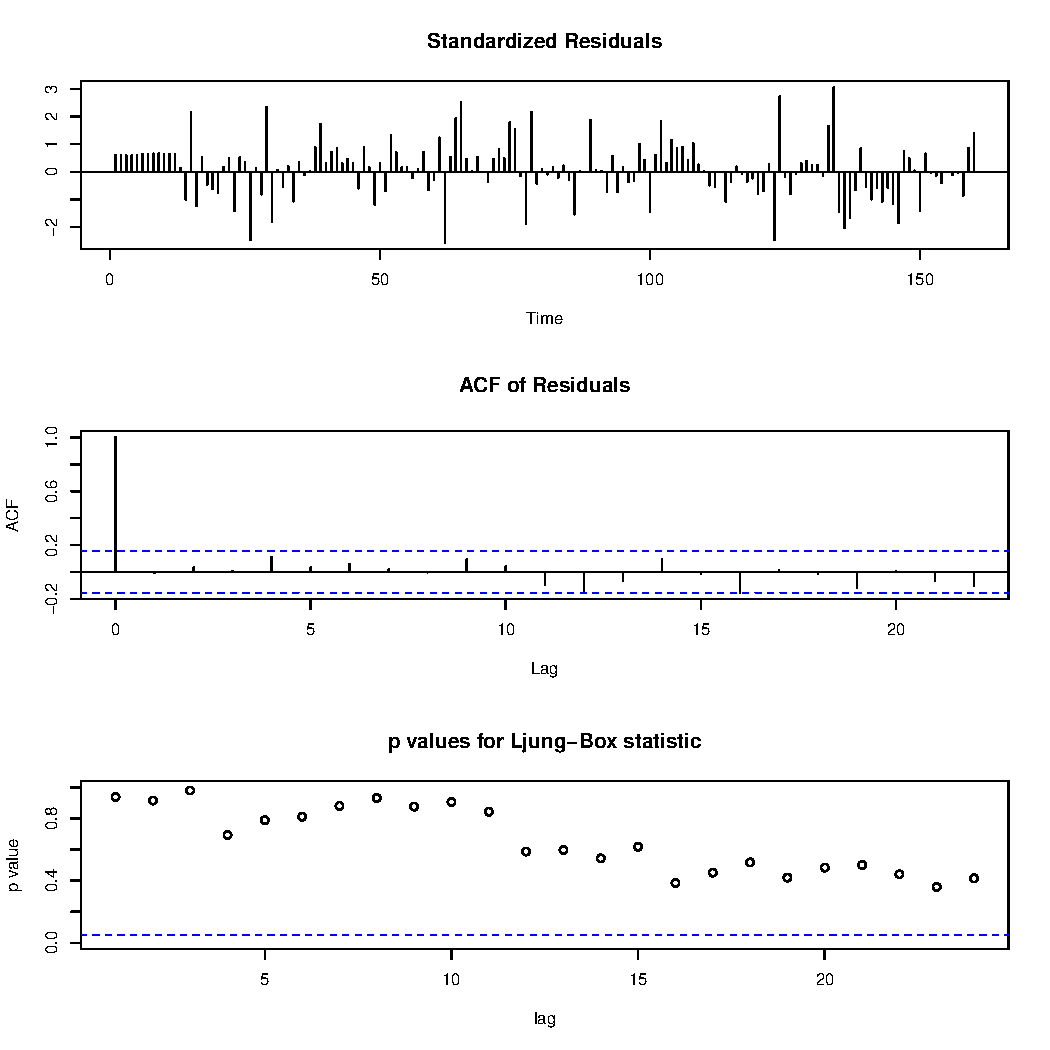
\includegraphics[width=\maxwidth]{figure/unnamed-chunk-19-1} 

}

\caption{\label{fig:sarima_resid13} Residuos - Test Portmanteau (Ljung-Box) SARIMA(4,0,0)(1,1,0)}\label{fig:unnamed-chunk-19}
\end{figure}


\end{knitrout}


Tras analizar estos estos tres modelos, y considerando los criterios de información como los dados por los estadísticos AIC, BIC, y Hannan Quinn, se elige como mejor modelo al SARIMA$(4,0,0)(1,1,0)_{12}$, ya que minimiza todos estos criterios, obteniendo $AIC=719.2606 $, $BIC=737.2439$, Hannan Quinn$=727.5325$. Además posee residuos que se comportan como ruido blanco, según las pruebas, de  varianza menor. Finalmente se puede representar este modelo mediante la siguiente ecuación:

\begin{equation}\label{eq:sarima}
(1- 2.659 B + 2.610 B^2 - 1.181 B^3  + 0.239 B^4)(1+ 0.738 B^{12})\Delta_{12} Y_t = \varepsilon_t
\end{equation}

\paragraph{Observación.} Los modelos hallados para cada uno de los cuatro clúster, siguiendo el mismo método descrito en esta sección, se encuentra en el apéndice \ref{ap:sarima}. Así mismo puede encontrar los coeficientes estimados, significancia de los mismos, y estadísticos de la bondad de ajuste, de los modelos de cada uno de las series asociadas a las estaciones que componen cada clúster. Se comentará más adelante, los resultados obtenidos en términos generales comparándolos con los modelos obtenidos usando los modelos SARIMAX que se presentan a continuación.






%%%%%%%%%%%%%%%%%%%%%%%%%%%%%%%%%%%%%%%%%%%%%%%%%%%%%%%%%%%%%%%%%%%%%%%%%%%%%%%%%%%
%%%%%%%%%%%%%%%%%%%%%%%%%%%     SARIMAX      %%%%%%%%%%%%%%%%%%%%%%%%%%%%%%%%%%%%%%
%%%%%%%%%%%%%%%%%%%%%%%%%%%%%%%%%%%%%%%%%%%%%%%%%%%%%%%%%%%%%%%%%%%%%%%%%%%%%%%%%%%


\newpage


\subsection{Modelo SARIMAX del Clúster}

En esta sección se buscará un segundo modelo que represente el Caudal para el clúster 1, para ello se considerará la serie \textit{medoide} del clúster, se halla una por cada clúster durante la ejecución del algoritmo CLARA, y se usará como representante del comportamiento del caudal de este clúster. Se aplicará un modelo SARIMAX usando como variables regresoras a la Precipitación, Temperatura Máxima, Temperatura Mínima, y Humedad Relativa medidas en la estación más cercana (geográficamente) a donde se midió el caudal asociado al medoide (ver figuras \ref{fig:mapa_vaz}, \ref{fig:mapa_clm}.





En este caso, el medoide correspondiente al clúster 1 es el de la estación MACHADINHO (217) (ver figura \ref{fig:sarimax_serie}), mientras que la estación de clima más cercana, asociada a esta, es CAMPOS NOVOS(83887) (ver figura \ref{fig:sarimax_serieCl}). Siguiendo la metodología propuesta por Box y Jenkins, cuya aplicación se encuentra a detalle en \citeauthor{novales1993econometria} \citeyear{novales1993econometria}, se obtiene lo siguiente.





\begin{knitrout}
\definecolor{shadecolor}{rgb}{0.969, 0.969, 0.969}\color{fgcolor}\begin{figure}[H]

{\centering 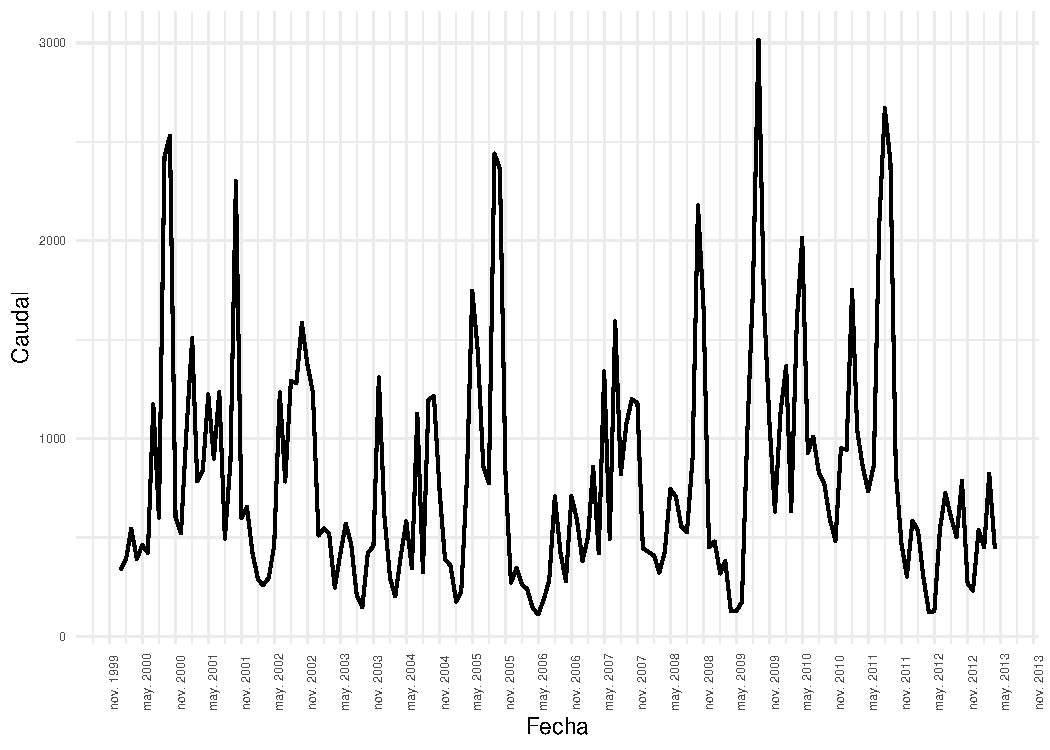
\includegraphics[width=\maxwidth]{figure/unnamed-chunk-22-1} 

}

\caption{\label{fig:sarimax_serie} Caudal - Estación Machadinho}\label{fig:unnamed-chunk-22}
\end{figure}


\end{knitrout}




\begin{knitrout}
\definecolor{shadecolor}{rgb}{0.969, 0.969, 0.969}\color{fgcolor}\begin{figure}[H]

{\centering 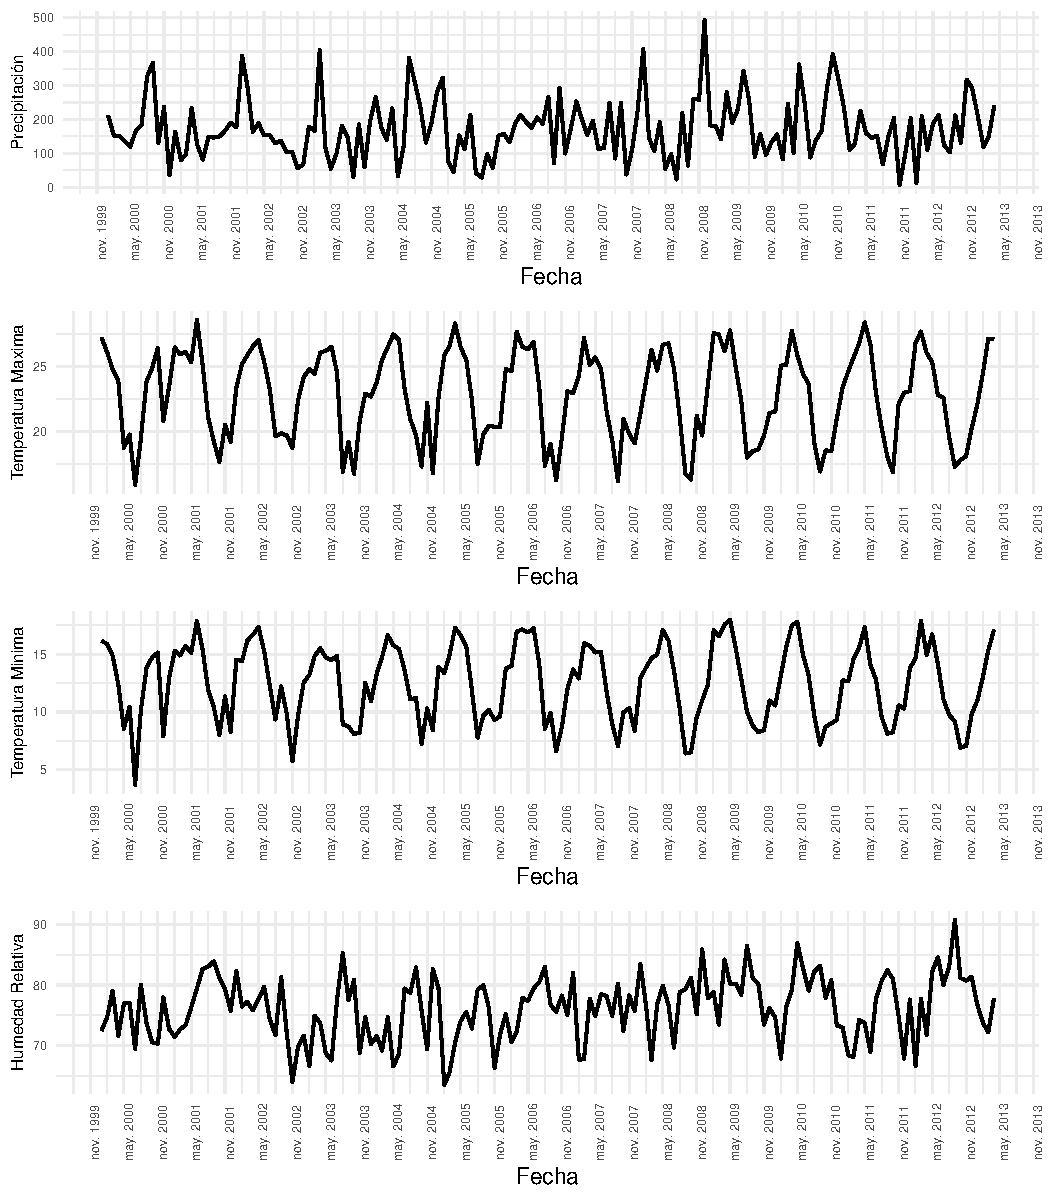
\includegraphics[width=\maxwidth]{figure/unnamed-chunk-23-1} 

}

\caption{\label{fig:sarimax_serieCl} Series Climáticas - Estación Campos Novos}\label{fig:unnamed-chunk-23}
\end{figure}


\end{knitrout}


\subsubsection{Preblanqueo de Series}

En primer lugar se necesita \textit{preblanquear} las series, tanto la serie de caudal, como las cuatro series asociadas a clima. Para ello se puede analizar sus funciones de autocorrelación y realizar el test de Dickey Fuller, a fin de identificar si es necesario diferenciar las series. 


\begin{itemize}
\item Para preblanquear la serie de caudales del la estación MACHADINHO (217) se analiza la función de autocorrelación  (ver figura \ref{fig:blan_acf_vz1}), que si bien es cierto presenta picos de periodicidad 12, estos no se encuentran fuera de las bandas de confianza, es decir, existe la posibilidad de que el proceso sea estacionario, para corroborarlo se puede ejecutar el test de Dickey Fuller (ver \ref{tab:dyf_vz1}), donde se obtiene un P-valor$=0.01$, es decir, se rechaza la existencia de raíces unitarias a favor de la hipótesis alternativa de que la serie es estacionaria, por lo tanto no es necesario diferenciar esta serie.




\begin{knitrout}
\definecolor{shadecolor}{rgb}{0.969, 0.969, 0.969}\color{fgcolor}\begin{figure}[H]

{\centering 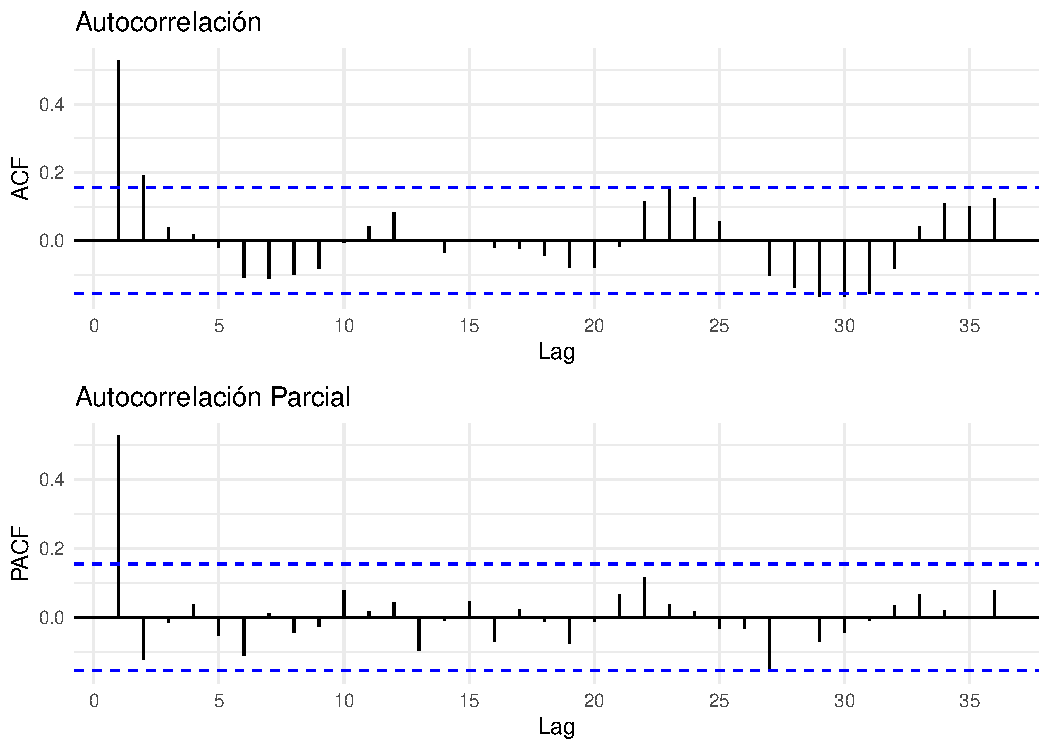
\includegraphics[width=\maxwidth]{figure/unnamed-chunk-24-1} 

}

\caption{\label{fig:blan_acf_vz1} Autocorrelación - Caudal}\label{fig:unnamed-chunk-24}
\end{figure}


\end{knitrout}
% \label{fig:blan_acf_vz1}


\begin{knitrout}
\definecolor{shadecolor}{rgb}{0.969, 0.969, 0.969}\color{fgcolor}\begin{kframe}
\begin{verbatim}
## 
## 	Augmented Dickey-Fuller Test
## 
## data:  VazTrain
## Dickey-Fuller = -5.2, Lag order = 5, p-value = 0.01
## alternative hypothesis: stationary
\end{verbatim}
\end{kframe}
\end{knitrout}
\label{tab:dyf_vz1}




\item De igual manera para el caso de la serie asociada a Precipitación, se observa una función de autocorrelación dentro de las bandas de confianza (ver figura \ref{fig:blan_acf_cl1}), con picos fuera de las bandas en los retardos 15 y 30, por lo que da cierto indicio de que esta serie es estacionaria, lo que puede corroborar aplicando el test de Dickey Fuller (\ref{tab:blan_dyf_cl1}), en el que se obtiene un P-valor$=0.01$, es decir, la serie asociada a Precipitación es también estacionaria.



\begin{knitrout}
\definecolor{shadecolor}{rgb}{0.969, 0.969, 0.969}\color{fgcolor}\begin{figure}[H]

{\centering 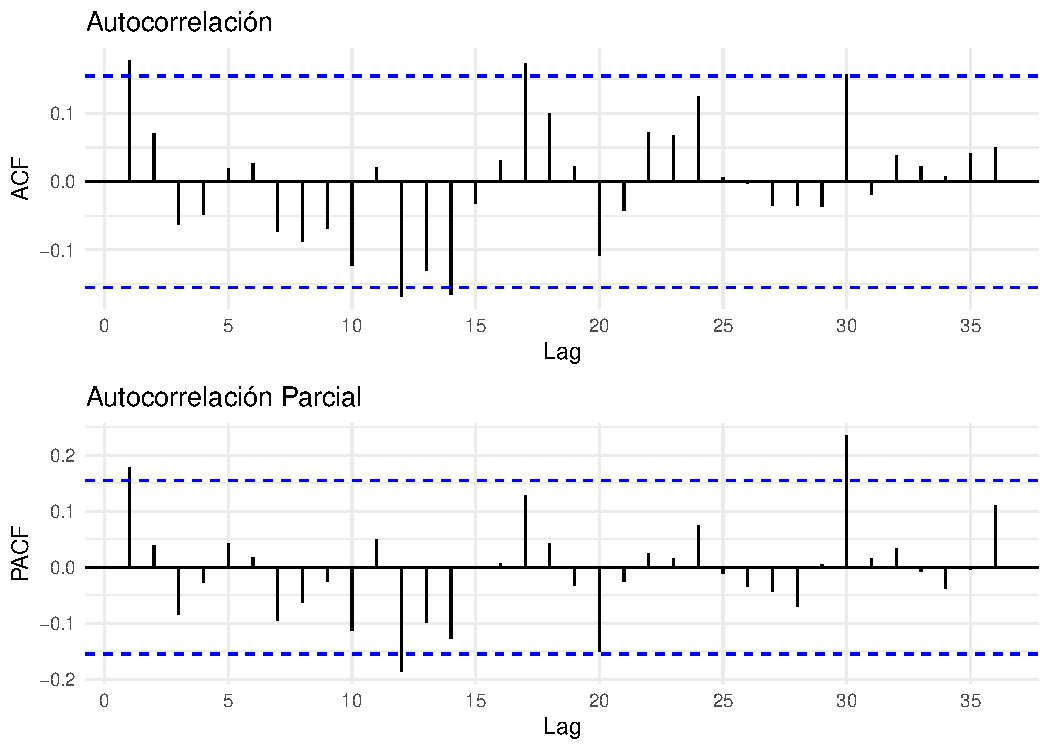
\includegraphics[width=\maxwidth]{figure/unnamed-chunk-26-1} 

}

\caption{\label{fig:blan_acf_cl1} Autocorrelación Precipitación}\label{fig:unnamed-chunk-26}
\end{figure}


\end{knitrout}


\begin{knitrout}
\definecolor{shadecolor}{rgb}{0.969, 0.969, 0.969}\color{fgcolor}\begin{kframe}
\begin{verbatim}
## 
## 	Augmented Dickey-Fuller Test
## 
## data:  Xtrain[, 1]
## Dickey-Fuller = -4.7, Lag order = 5, p-value = 0.01
## alternative hypothesis: stationary
\end{verbatim}
\end{kframe}
\end{knitrout}
\label{tab:blan_dyf_cl1}


\item Para el caso de la serie asociada a Temperatura Máxima y Mínima, se observa un comportamiento similar de sus funciones de autocorrelación (ver figura \ref{fig:blan_acf_cl2}, \ref{fig:blan_acf_cl3}), ambas con picos periódicos fuera de las bandas de confianza, lo que podría indicar la necesidad de diferenciar estas series estacionalmente.

\begin{knitrout}
\definecolor{shadecolor}{rgb}{0.969, 0.969, 0.969}\color{fgcolor}\begin{figure}[H]

{\centering 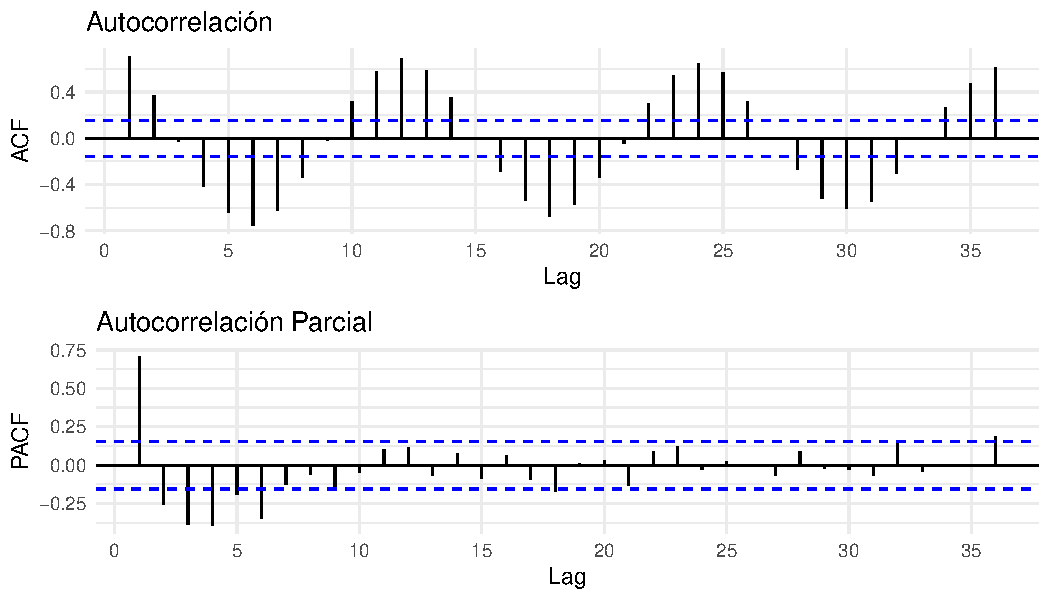
\includegraphics[width=\maxwidth]{figure/unnamed-chunk-28-1} 

}

\caption{\label{fig:blan_acf_cl2} Autocorrelación Temperatura Máxima}\label{fig:unnamed-chunk-28}
\end{figure}


\end{knitrout}


\begin{knitrout}
\definecolor{shadecolor}{rgb}{0.969, 0.969, 0.969}\color{fgcolor}\begin{figure}[H]

{\centering 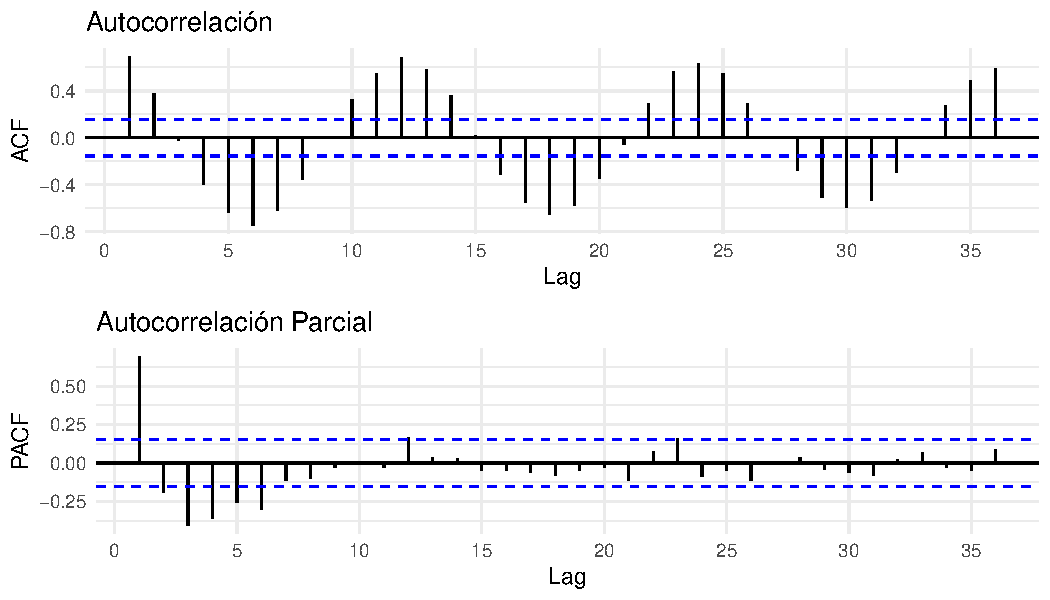
\includegraphics[width=\maxwidth]{figure/unnamed-chunk-29-1} 

}

\caption{\label{fig:blan_acf_cl3} Autocorrelación Temperatura Mínima}\label{fig:unnamed-chunk-29}
\end{figure}


\end{knitrout}


\item Finalmente, analizando la serie asociada a Humedad Relativa (ver figura \ref{fig:blan_acf_cl4}), se observa que la función de autocorrelación presenta picos relativamente pequeños periódicos cada 12 retardos, que apenas salen de las bandas, por lo que es posible que la serie sea estacionaria, para corroborarlo se realiza el test de Dickey Fuller, donde se obtiene un P-valor$=0.01$, es decir, se concluye que la serie es estacionaria, y por lo tanto no es necesario diferenciar esta serie.

\begin{knitrout}
\definecolor{shadecolor}{rgb}{0.969, 0.969, 0.969}\color{fgcolor}\begin{kframe}
\begin{verbatim}
## 
## 	Augmented Dickey-Fuller Test
## 
## data:  Xtrain[, 4]
## Dickey-Fuller = -5.8, Lag order = 5, p-value = 0.01
## alternative hypothesis: stationary
\end{verbatim}
\end{kframe}
\end{knitrout}


\begin{knitrout}
\definecolor{shadecolor}{rgb}{0.969, 0.969, 0.969}\color{fgcolor}\begin{figure}[H]

{\centering 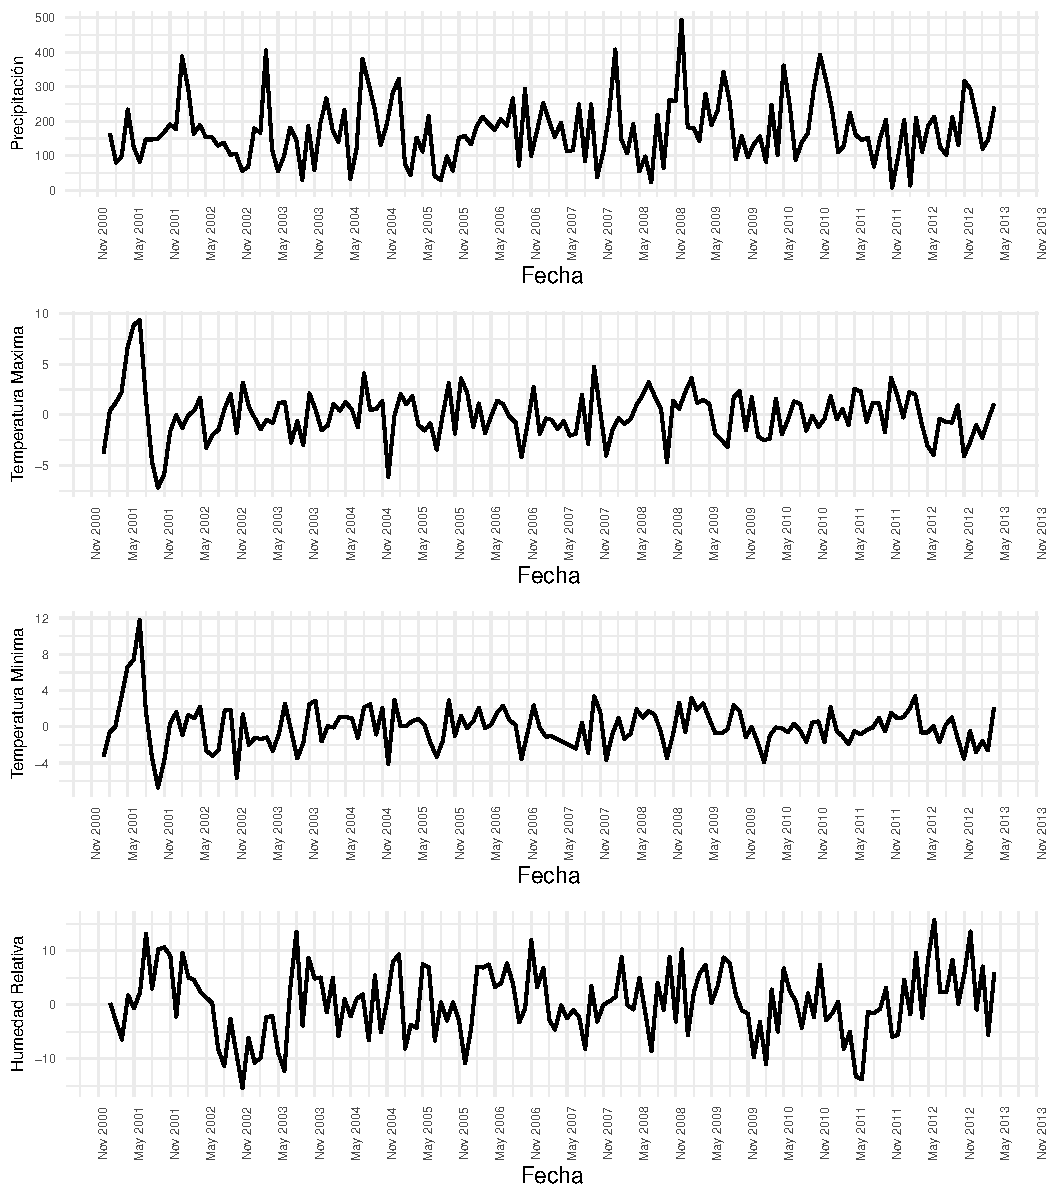
\includegraphics[width=\maxwidth]{figure/unnamed-chunk-31-1} 

}

\caption{\label{fig:blan_acf_cl4} Autocorrelación Humedad Relativa}\label{fig:unnamed-chunk-31}
\end{figure}


\end{knitrout}



\end{itemize}

Como se puede observar en la figura \ref{fig:blanqueadas}, se ha obtenido series estacionarias mediante el proceso de preblanqueo de las series tanto de caudales como climáticas. Por lo que se puede pasar al siguiente paso de la metodología Box y Jenkins para el modelo SARIMAX.



%%%%%%%%%%%%%%%%%%%%%%%%%%%%%%%%%%%%%%%%%%%%%%%%%%%
%%%%%%%%%% Series Preblanqueadas %%%%%%%%%%%%%%%%%%

\begin{knitrout}
\definecolor{shadecolor}{rgb}{0.969, 0.969, 0.969}\color{fgcolor}\begin{figure}[H]

{\centering 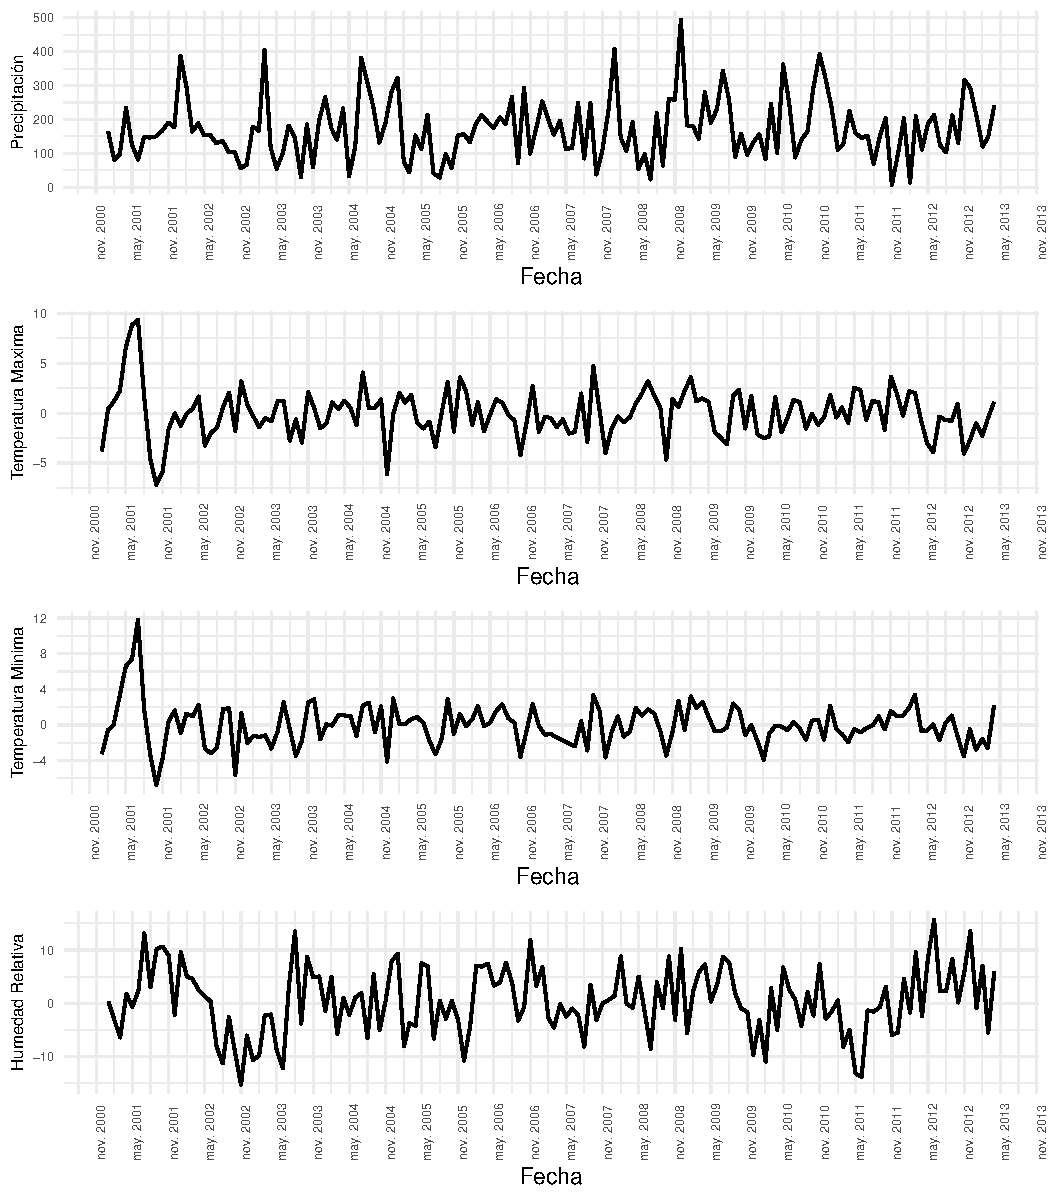
\includegraphics[width=\maxwidth]{figure/unnamed-chunk-32-1} 

}

\caption{\label{fig:blanqueadas} Series Blanqueadas}\label{fig:unnamed-chunk-32}
\end{figure}


\end{knitrout}







%%%%%%%%%%%%%%%%%%%%%%%%%%%%%%%%%%%%%%%%%%%%%%%%%%%%%%
%%%%%    Funciones de Correlacion Cruzada   %%%%%%%%%%
%%%%%%%%%%%%%%%%%%%%%%%%%%%%%%%%%%%%%%%%%%%%%%%%%%%%%%






\begin{knitrout}
\definecolor{shadecolor}{rgb}{0.969, 0.969, 0.969}\color{fgcolor}\begin{figure}[H]

{\centering 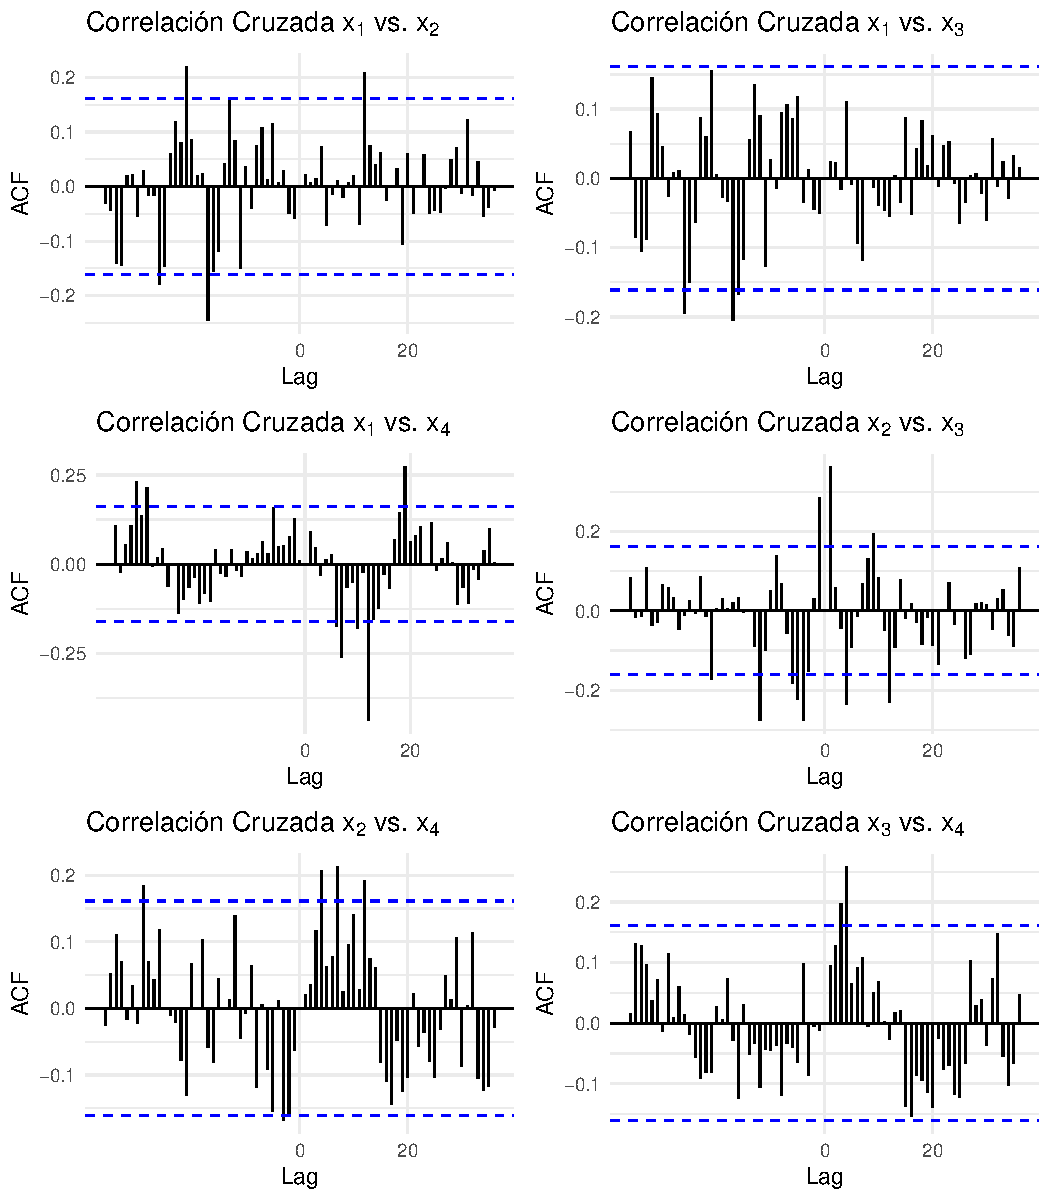
\includegraphics[width=\maxwidth]{figure/unnamed-chunk-34-1} 

}

\caption{\label{fig:cc_exogenas} Corrleaciones Cruzadas - Variables Exógenas}\label{fig:unnamed-chunk-34}
\end{figure}


\end{knitrout}


\begin{knitrout}
\definecolor{shadecolor}{rgb}{0.969, 0.969, 0.969}\color{fgcolor}\begin{figure}[H]

{\centering 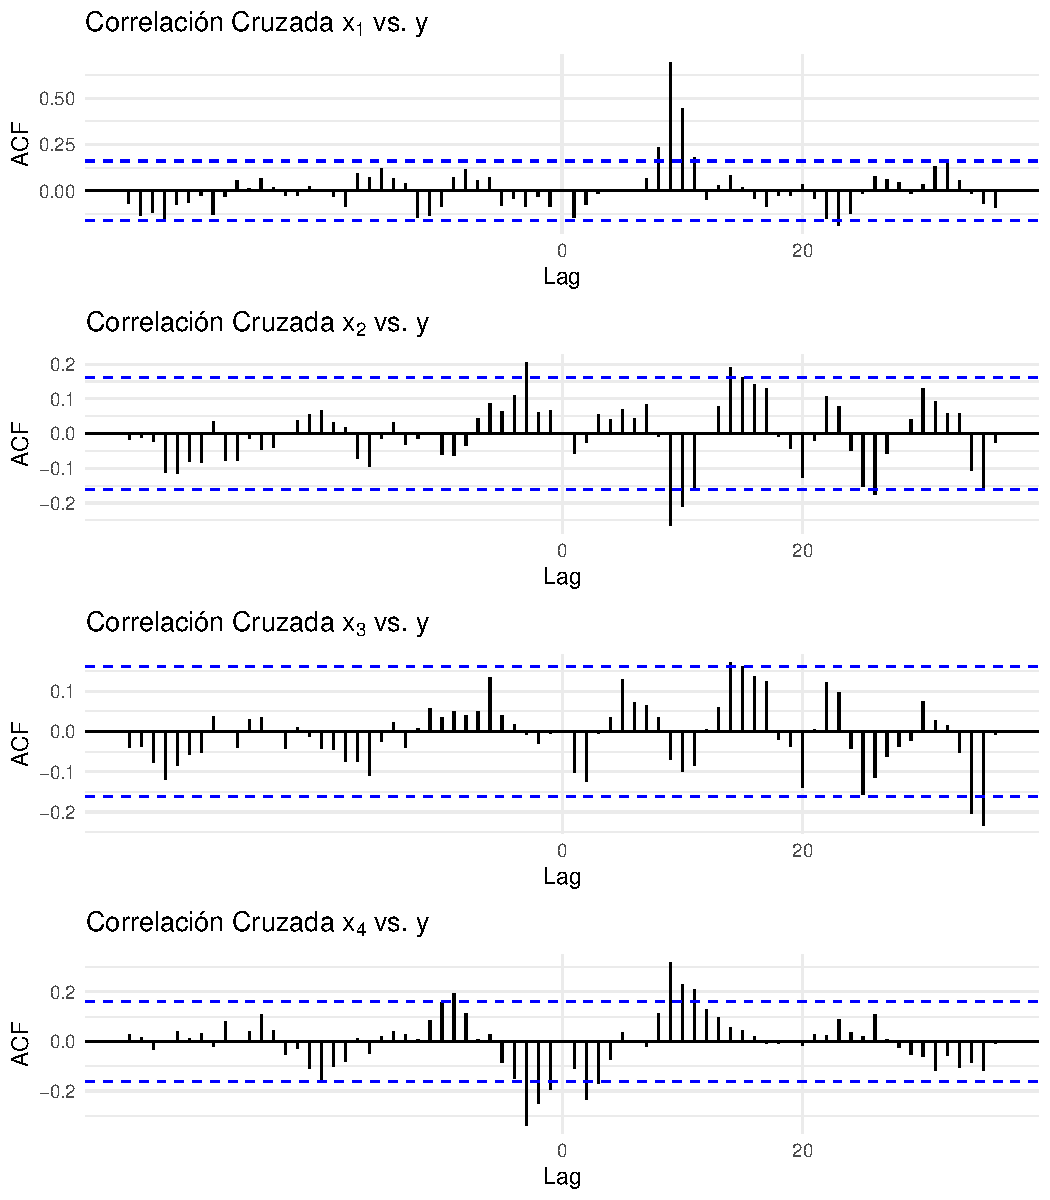
\includegraphics[width=\maxwidth]{figure/unnamed-chunk-35-1} 

}

\caption{\label{fig:cc_output} Corrleaciones Cruzadas - Caudal vs. Variables Exógenas}\label{fig:unnamed-chunk-35}
\end{figure}


\end{knitrout}




%%%%%%%%%%%%%%%%%%%%%%%%%%%%%%%%%%%%%%%%%%%%%%%%%%%%%
\newpage
\subsubsection{Identificación de Funciones de Respuesta al Impulso}

Siguiendo la metodología de identificación de este modelo, se pasa a la etapa de identificación de las funciones de respuesta al impulso asociadas a las variables climáticas. Considerando lo siguiente:

\begin{itemize}
\item $v^{(1)}(B)$ : Función de respuesta al impulso asociada a la Precipitación $x^{(1)}_t$.
\item $v^{(2)}(B)$ : Función de respuesta al impulso asociada a la Temperatura Máxima $x^{(2)}_t$.
\item $v^{(3)}(B)$ : Función de respuesta al impulso asociada a la Temperatura Mínima $x^{(3)}_t$.
\item $v^{(4)}(B)$ : Función de respuesta al impulso asociada a la Humedad Relativa $x^{(4)}_t$.
\end{itemize}


Como se mostró en el capítulo anterior, esta etapa consiste de hallar modelos SARMA para cada variable exógena, es decir al final de esta etapa se obtienen modelos del tipo:


$$\frac{ \phi_x^{(k)}(B) \Phi_x^{(k)}(B) }{\theta_x^{(k)}(B) \Theta_x^{(k)}(B)} x^{(k)}_t= \alpha^{(k)}_t $$

donde $\alpha^{(k)}_t$ es un r.b. de varianza $\sigma^2_k$, para $k=1,2,3,4$.

A continuación se muestran los 4 modelos SARMA obtenidos, sus coeficientes, significancia, bondad de ajuste y validación de residuos.

\begin{enumerate}

\item Siguiendo la metodología Box y Jenkins clásica, se obtuvo, para la variable Precipitación, un modelo SARMA con parámetros $p=1$ , $P=2$, $q=0$ y $Q=1$. Se muestran los coeficientes de este modelo y su significancia en la tabla \ref{tab:sarma_precip}, se muestra además, en la figura \ref{fig:sarma_precip}, el análisis de los residuos, donde de acuerdo a los P-valores del estadístico de Ljung-Box (Portmanteau), se concluye sigue que los residuos del modelo se comportan como un r.b.

\begin{knitrout}
\definecolor{shadecolor}{rgb}{0.969, 0.969, 0.969}\color{fgcolor}\begin{table}

\caption{\label{tab:model_x1}\label{tab:sarma_precip}Modelo SARMA(1,0)(2,1) - Precipitación}
\centering
\begin{threeparttable}
\begin{tabular}[t]{lrrrrl}
\toprule
Coef & Estimate & Std.Error & z-value & Pr(>|z|) & Signif\\
\midrule
\rowcolor{gray!6}  ar1 & 0.1740 & 0.0808 & 2.153 & 0.0313 & *\\
sar1 & 0.7661 & 0.1173 & 6.529 & 0.0000 & ***\\
\rowcolor{gray!6}  sma1 & -1.0276 & 0.1352 & -7.601 & 0.0000 & ***\\
sma2 & 0.4029 & 0.1039 & 3.879 & 0.0001 & ***\\
\rowcolor{gray!6}  intercept & 170.3718 & 10.9360 & 15.579 & 0.0000 & ***\\
\bottomrule
\end{tabular}
\begin{tablenotes}
\item \textit{Resumen:} 
\item sigma\textasciicircum{}2 = 6957.57, loglikelihood = -864.64, AIC = 1741.28, BIC =1759.26, Hannan-Quinn =1749.55
\end{tablenotes}
\end{threeparttable}
\end{table}


\end{knitrout}



\begin{knitrout}
\definecolor{shadecolor}{rgb}{0.969, 0.969, 0.969}\color{fgcolor}\begin{figure}[H]

{\centering 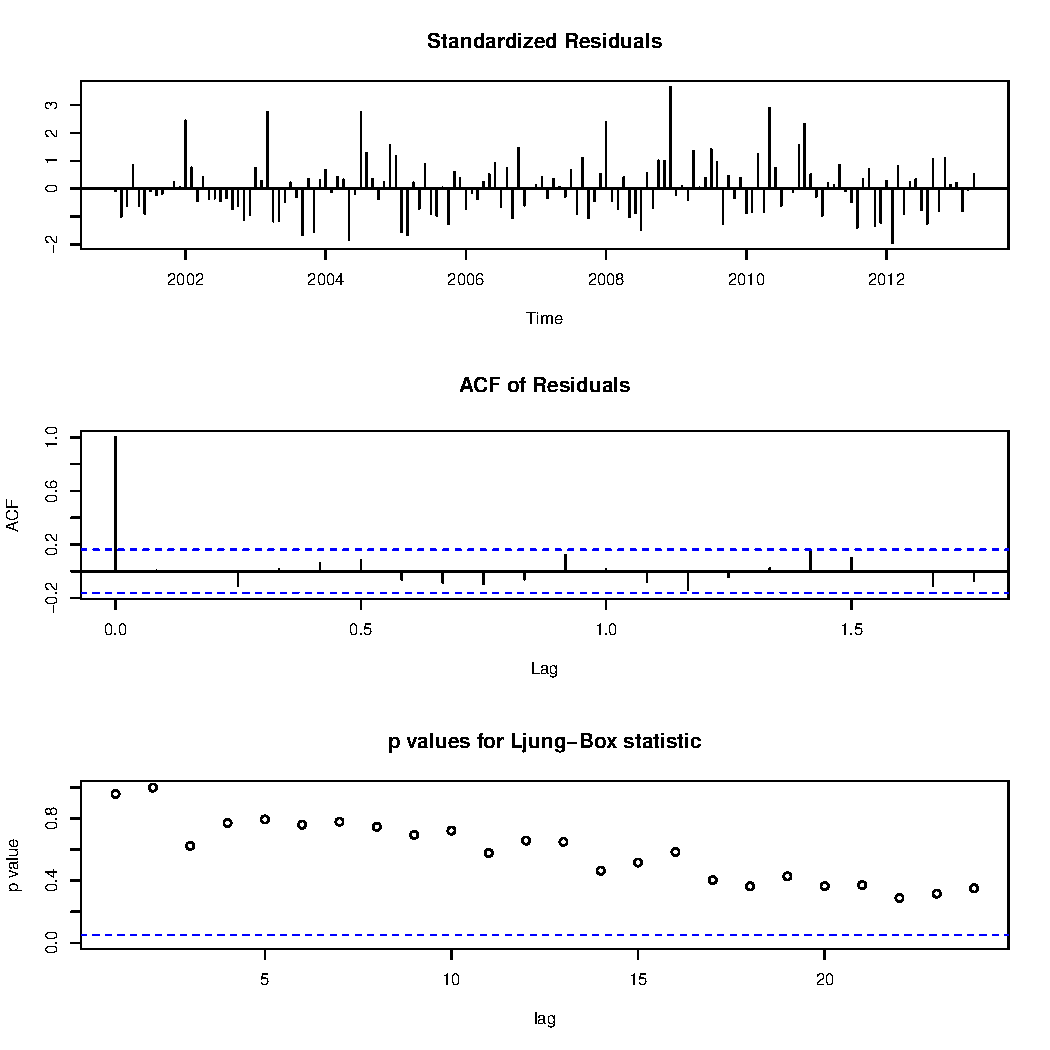
\includegraphics[width=\maxwidth]{figure/unnamed-chunk-36-1} 

}

\caption{\label{fig:sarma_precip} Residuos SARMA(1,0)(2,1) - Precipitación}\label{fig:unnamed-chunk-36}
\end{figure}


\end{knitrout}






\item De igual manera, para la variable Temperatura Máxima se obtuvo un modelo SARMA con parámetros $p=4$ , $P=0$, $q=0$ y $Q=2$. Se muestran los coeficientes de este modelo y su significancia en la tabla \ref{tab:sarma_tmax}, se muestra además, en la figura \ref{fig:sarma_tmax}, el análisis de los residuos, donde de acuerdo a los P-valores del estadístico de Ljung-Box (Portmanteau), se concluye sigue que los residuos del modelo se comportan como un r.b.

\begin{knitrout}
\definecolor{shadecolor}{rgb}{0.969, 0.969, 0.969}\color{fgcolor}\begin{table}

\caption{\label{tab:model_x2}\label{tab:sarma_tmax}Modelo SARMA(4,0)(0,2) - Temperatura Máxima}
\centering
\begin{threeparttable}
\begin{tabular}[t]{lrrrrl}
\toprule
Coef & Estimate & Std.Error & z-value & Pr(>|z|) & Signif\\
\midrule
\rowcolor{gray!6}  ar1 & 0.3445 & 0.0737 & 4.673 & 0.0000 & ***\\
ar4 & -0.3300 & 0.0708 & -4.657 & 0.0000 & ***\\
\rowcolor{gray!6}  sma1 & -0.9512 & 0.1103 & -8.620 & 0.0000 & ***\\
sma2 & 0.1802 & 0.1092 & 1.651 & 0.0988 & .\\
\bottomrule
\end{tabular}
\begin{tablenotes}
\item \textit{Resumen:} 
\item sigma\textasciicircum{}2 = 2.75, loglikelihood = -292, AIC = 594.01, BIC =608.99, Hannan-Quinn =600.9
\end{tablenotes}
\end{threeparttable}
\end{table}


\end{knitrout}






\begin{knitrout}
\definecolor{shadecolor}{rgb}{0.969, 0.969, 0.969}\color{fgcolor}\begin{figure}[H]

{\centering 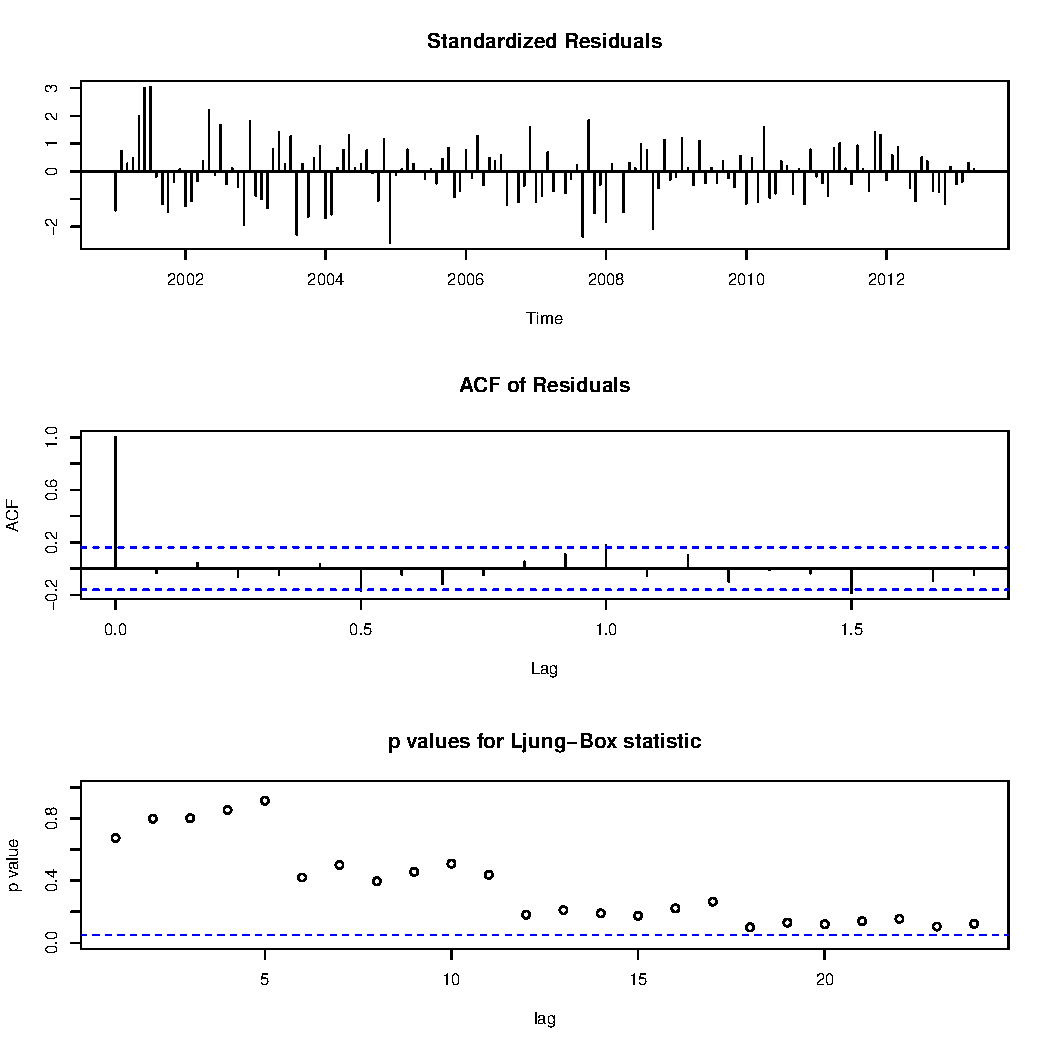
\includegraphics[width=\maxwidth]{figure/unnamed-chunk-37-1} 

}

\caption{\label{fig:sarma_tmax} Residuos SARMA(4,0)(0,2) - Temperatura Máxima}\label{fig:unnamed-chunk-37}
\end{figure}


\end{knitrout}







\item Para la variable Temperatura Mínima se obtuvo un modelo SARMA con parámetros $p=2$ , $P=2$, $q=2$ y $Q=1$. Se muestran los coeficientes de este modelo y su significancia en la tabla \ref{tab:sarma_tmin}, se muestra además, en la figura \ref{fig:sarma_tmin}, el análisis de los residuos, donde de acuerdo a los P-valores del estadístico de Ljung-Box (Portmanteau), se concluye sigue que los residuos del modelo se comportan como un r.b.

\begin{knitrout}
\definecolor{shadecolor}{rgb}{0.969, 0.969, 0.969}\color{fgcolor}\begin{table}

\caption{\label{tab:model_x3}\label{tab:sarma_tmin}Modelo SARMA(2,2)(2,1) - Temperatura Mínima}
\centering
\begin{threeparttable}
\begin{tabular}[t]{lrrrrl}
\toprule
Coef & Estimate & Std.Error & z-value & Pr(>|z|) & Signif\\
\midrule
\rowcolor{gray!6}  ar1 & 1.4773 & 0.1401 & 10.5418 & 0.0000 & ***\\
ar2 & -0.8168 & 0.1221 & -6.6882 & 0.0000 & ***\\
\rowcolor{gray!6}  ma1 & -1.1716 & 0.1778 & -6.5899 & 0.0000 & ***\\
ma2 & 0.4973 & 0.1810 & 2.7470 & 0.0060 & **\\
\rowcolor{gray!6}  sar2 & -0.1144 & 0.1217 & -0.9397 & 0.3474 & \\
\addlinespace
sma1 & -0.7657 & 0.0909 & -8.4195 & 0.0000 & ***\\
\bottomrule
\end{tabular}
\begin{tablenotes}
\item \textit{Resumen:} 
\item sigma\textasciicircum{}2 = 3.02, loglikelihood = -298.25, AIC = 610.49, BIC =631.47, Hannan-Quinn =620.14
\end{tablenotes}
\end{threeparttable}
\end{table}


\end{knitrout}


\begin{knitrout}
\definecolor{shadecolor}{rgb}{0.969, 0.969, 0.969}\color{fgcolor}\begin{figure}[H]

{\centering 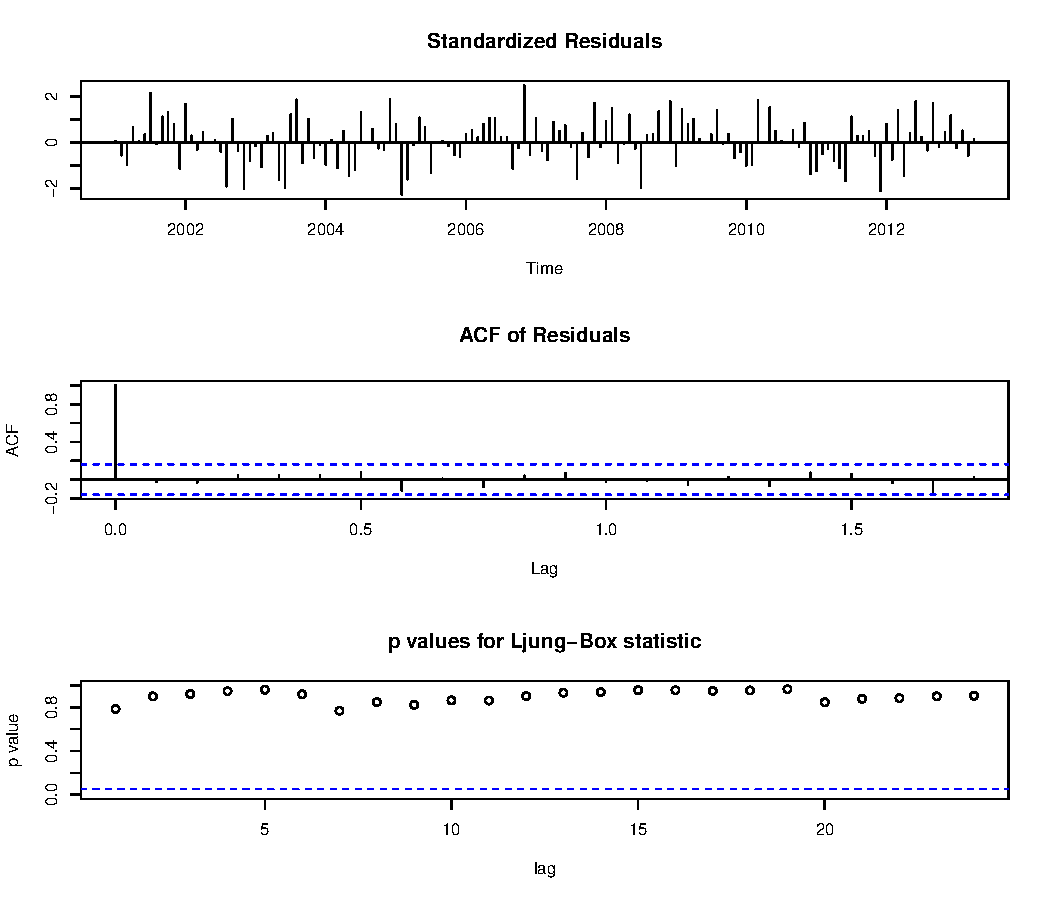
\includegraphics[width=\maxwidth]{figure/unnamed-chunk-38-1} 

}

\caption{\label{fig:sarma_tmin} Residuos SARMA(2,2)(2,1) - Temperatura Mínima}\label{fig:unnamed-chunk-38}
\end{figure}


\end{knitrout}






\item Finalmente para la variable Humedad Relativa se obtuvo un modelo SARMA con parámetros $p=2$ , $P=3$, $q=0$ y $Q=0$. Se muestran los coeficientes de este modelo y su significancia en la tabla \ref{tab:sarma_humed}, se muestra además, en la figura \ref{fig:sarma_humed}, el análisis de los residuos, donde de acuerdo a los P-valores del estadístico de Ljung-Box (Portmanteau), se concluye sigue que los residuos del modelo se comportan como un r.b.

\begin{knitrout}
\definecolor{shadecolor}{rgb}{0.969, 0.969, 0.969}\color{fgcolor}\begin{table}

\caption{\label{tab:model_x4}\label{tab:sarma_humed}Modelo SARMA(2,0)(3,0) - Humedad Relativa}
\centering
\begin{threeparttable}
\begin{tabular}[t]{lrrrrl}
\toprule
Coef & Estimate & Std.Error & z-value & Pr(>|z|) & Signif\\
\midrule
\rowcolor{gray!6}  ar1 & 0.2121 & 0.0799 & 2.655 & 0.0079 & **\\
ar2 & 0.2238 & 0.0801 & 2.796 & 0.0052 & **\\
\rowcolor{gray!6}  sar1 & -0.7224 & 0.0856 & -8.443 & 0.0000 & ***\\
sar2 & -0.4171 & 0.0986 & -4.230 & 0.0000 & ***\\
\rowcolor{gray!6}  sar3 & -0.1639 & 0.0926 & -1.769 & 0.0769 & .\\
\bottomrule
\end{tabular}
\begin{tablenotes}
\item \textit{Resumen:} 
\item sigma\textasciicircum{}2 = 22.99, loglikelihood = -443.05, AIC = 898.1, BIC =916.08, Hannan-Quinn =906.37
\end{tablenotes}
\end{threeparttable}
\end{table}


\end{knitrout}


\begin{knitrout}
\definecolor{shadecolor}{rgb}{0.969, 0.969, 0.969}\color{fgcolor}\begin{figure}[H]

{\centering 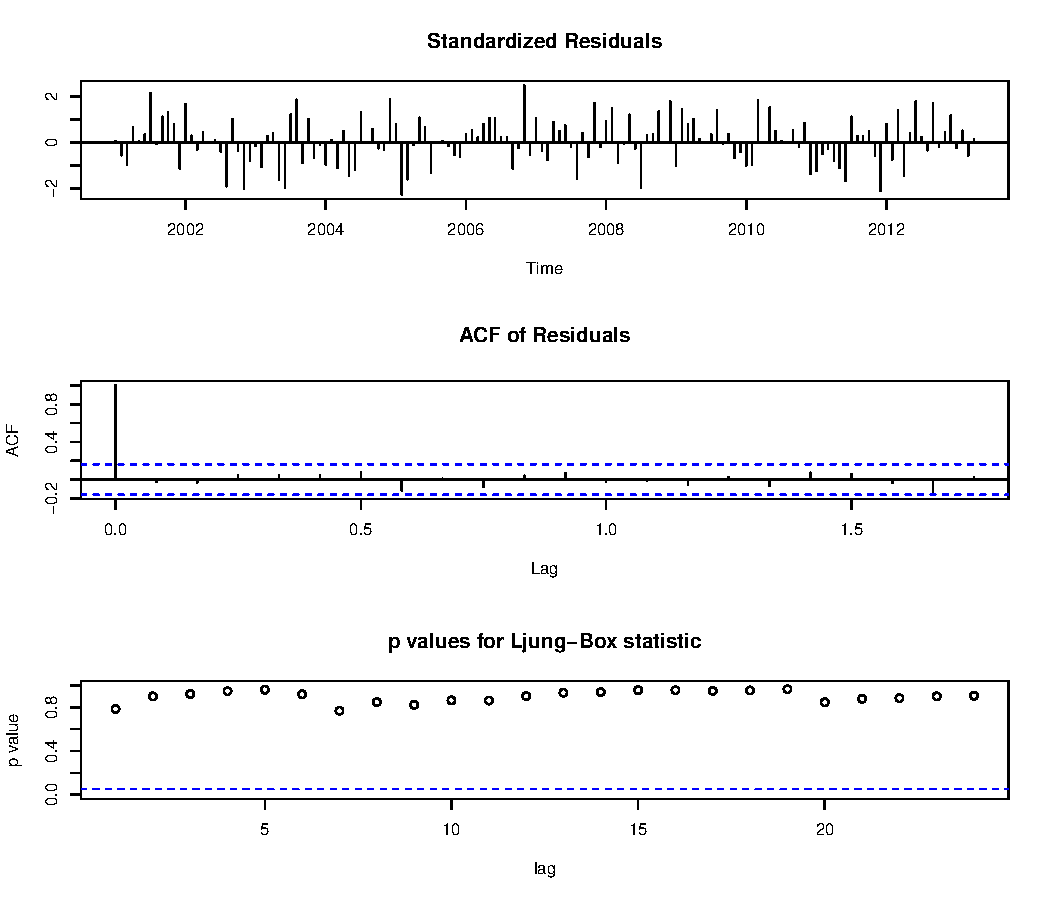
\includegraphics[width=\maxwidth]{figure/unnamed-chunk-39-1} 

}

\caption{\label{fig:sarma_humed} Residuos SARMA(2,0)(3,0) - Humedad Relativa}\label{fig:unnamed-chunk-39}
\end{figure}


\end{knitrout}


\end{enumerate}








%%%%%%%%%%%%%%%%%%%%%%%%%%%%%%%%%%%%%%%%%%%%%%%%
%%%%%%%%%%%%%%%%%%%%%%%%%%%%%%%%%%%%%%%%%%%%%%%%





Ahora se puede pasar al paso 3 de la metodología \ref{sec:metod_sarimax}, que consiste de identificar los órdenes de los polinomios $\delta^{(k)}(B)$, $\omega^{(k)}(B)$ que componen las funciones de respuesta al impulso $v^{(k)}(B)$ asociadas a $x_t^{(k)}$. Para ello un primer paso consiste de estimar los coeficientes $v_j^{(k)}$ de las funciones de respuesta al impulso, esto a partir de los valores de la función de correlación cruzada entre $\alpha_t^{(k)}$, hallada  en el paso anterior, y $\beta^{(k)}$ que resulta de aplicar el modelo SARMA de la $k$-ésima variable, pero a la serie $y_t$, es decir:

$$\beta^{(k)} = \frac{ \phi_x^{(k)}(B) \Phi_x^{(k)}(B) }{\theta_x^{(k)}(B) \Theta_x^{(k)}(B)} y_t$$


Los coeficientes estimados de $v_j^{(k)}$ vienen dados por:

$$\hat v_j^{(k)} = \hat\rho_{\alpha\beta}(j) \frac{\hat\sigma_{\beta^{(k)}}}{\hat\sigma_\alpha} $$

Se muestran a continuación, los coeficientes estimados de $v_j^{(k)}$ para cada una de las 4 variables climáticas


\begin{enumerate}


\item Para la variable Precipitación $x_t^{(1)}$, se obtienen los valores estimados de $v_j^{(1)}$ para $j=-36,\dots , 0, \dots, 36$, se representan en la figura \ref{fig:vj1}. Se puede observar en la figura \ref{fig:vj1} que los coeficientes estimados siguen un comportamiento sinusoidal, conducta usual de sucesiones que son solución de ecuaciones en diferencias de segundo grado, por lo tanto se considera $m=2$, retardos del polinomio $\delta^{(1)}(B)$. Como los primeros valores de $v_j^{(1)}$ no son próximos a cero, se toma $b=0$. Cabe recalcar que la función de correlación cruzada tiene un pico en $j=-8$, es decir, la máxima correlación se da entre $y_t$ y $x_{t+8}^{(1)}$, por lo que podría ser necesario considerar $n=8$ retardos del polinomio $\omega^{(1)}(B)$.



\begin{knitrout}
\definecolor{shadecolor}{rgb}{0.969, 0.969, 0.969}\color{fgcolor}\begin{figure}[H]

{\centering 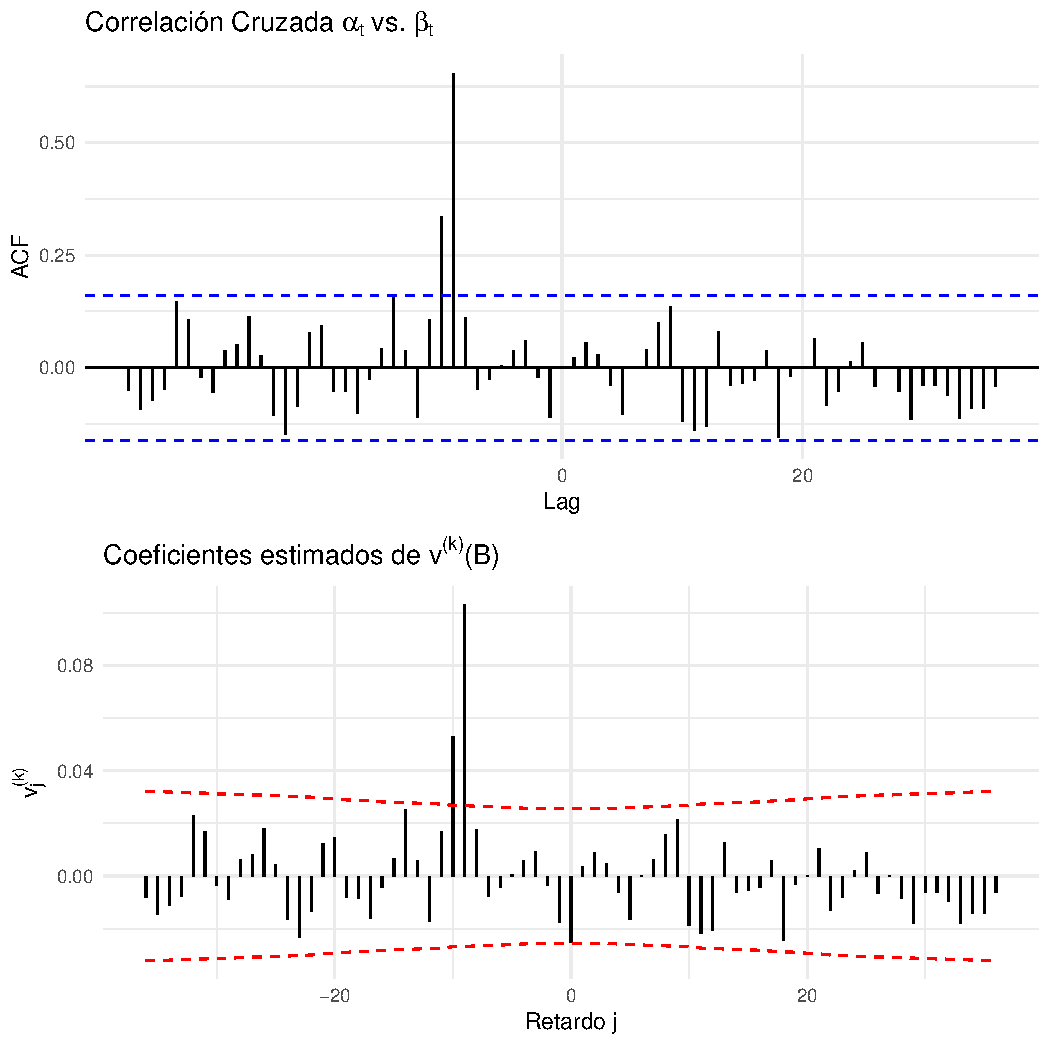
\includegraphics[width=\maxwidth]{figure/unnamed-chunk-41-1} 

}

\caption{\label{fig:vj1} Coeficientes $v_j$ estimados - Precipitación}\label{fig:unnamed-chunk-41}
\end{figure}


\end{knitrout}



\item Para la variable Temperatura Máxima $x_t^{(2)}$, se observa que los coeficientes $\hat v_j^{(2)}$ se encuentran dentro de las bandas de confianza, y no siguen un patron en específico (figura \ref{fig:vj2}). Así, consideramos $m=0$, mientras que como todos los coeficientes $\hat v_j^{(2)}$ se encuentran dentro de las bandas de confianza, entonces se toman $b=0$, y $n=0$. Es decir, se ingresa esta variable sin retardos, como si se tratara de una regresión múltiple.




\begin{knitrout}
\definecolor{shadecolor}{rgb}{0.969, 0.969, 0.969}\color{fgcolor}\begin{figure}[H]

{\centering 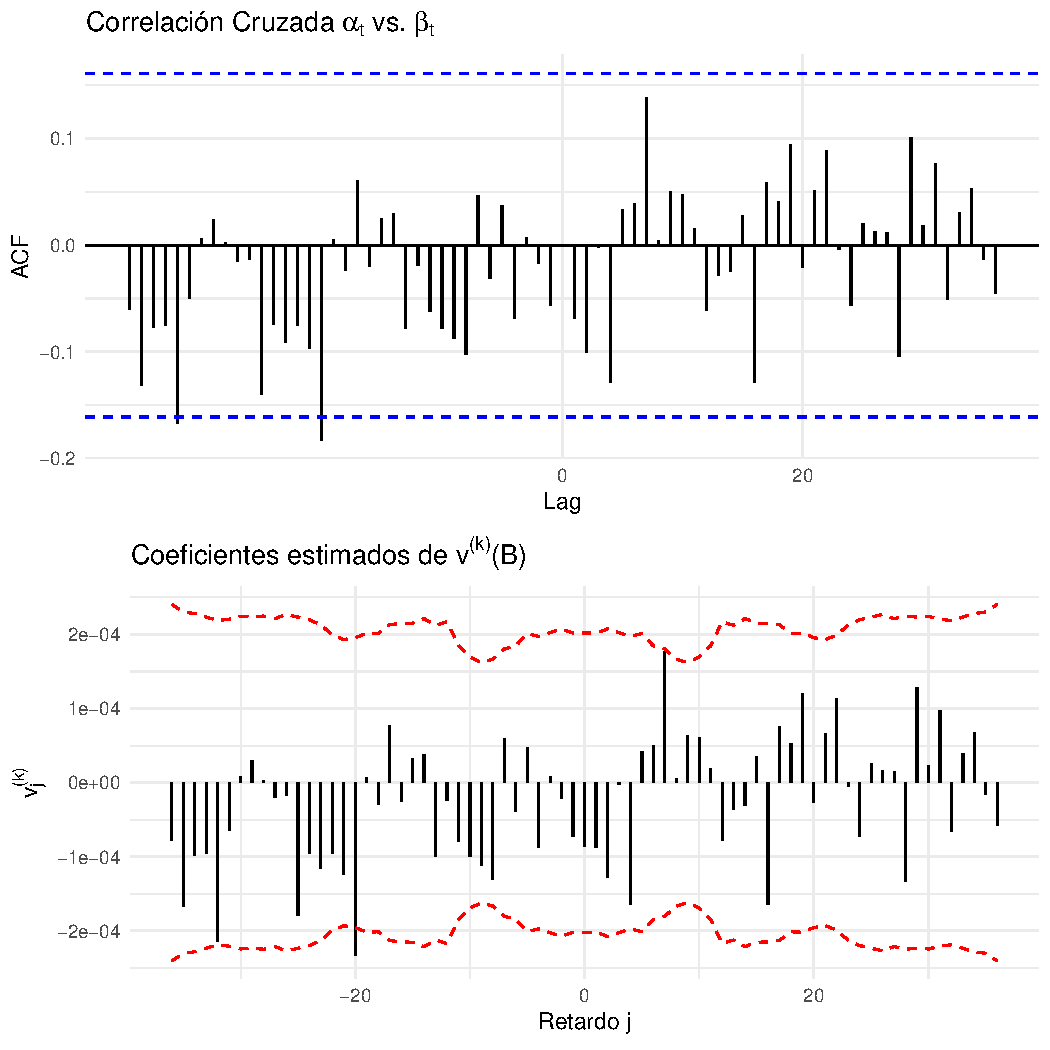
\includegraphics[width=\maxwidth]{figure/unnamed-chunk-42-1} 

}

\caption{\label{fig:vj2} Coeficientes $v_j$ estimados - Temperatura Máxima}\label{fig:unnamed-chunk-42}
\end{figure}


\end{knitrout}


\item Para la variable Temperatura Mínima $x_t^{(3)}$, se observa que los coeficientes $\hat v_j^{(3)}$, de manera similar a la Temperatura Mínima, se encuentran dentro de las bandas de confianza a excepción de los retardos $j=4$ y $j=-20$, aunque es descartado por el principio de parsimonia (ya que hace que el modelo tenga demasiados coeficientes a estimar y se vuelva más complejo), por lo que se toma $n=4$. Además no siguien un patrón claro (figura \ref{fig:vj3}), por lo tanto se toman $m=0$, $b=0$. 


\begin{knitrout}
\definecolor{shadecolor}{rgb}{0.969, 0.969, 0.969}\color{fgcolor}\begin{figure}[H]

{\centering 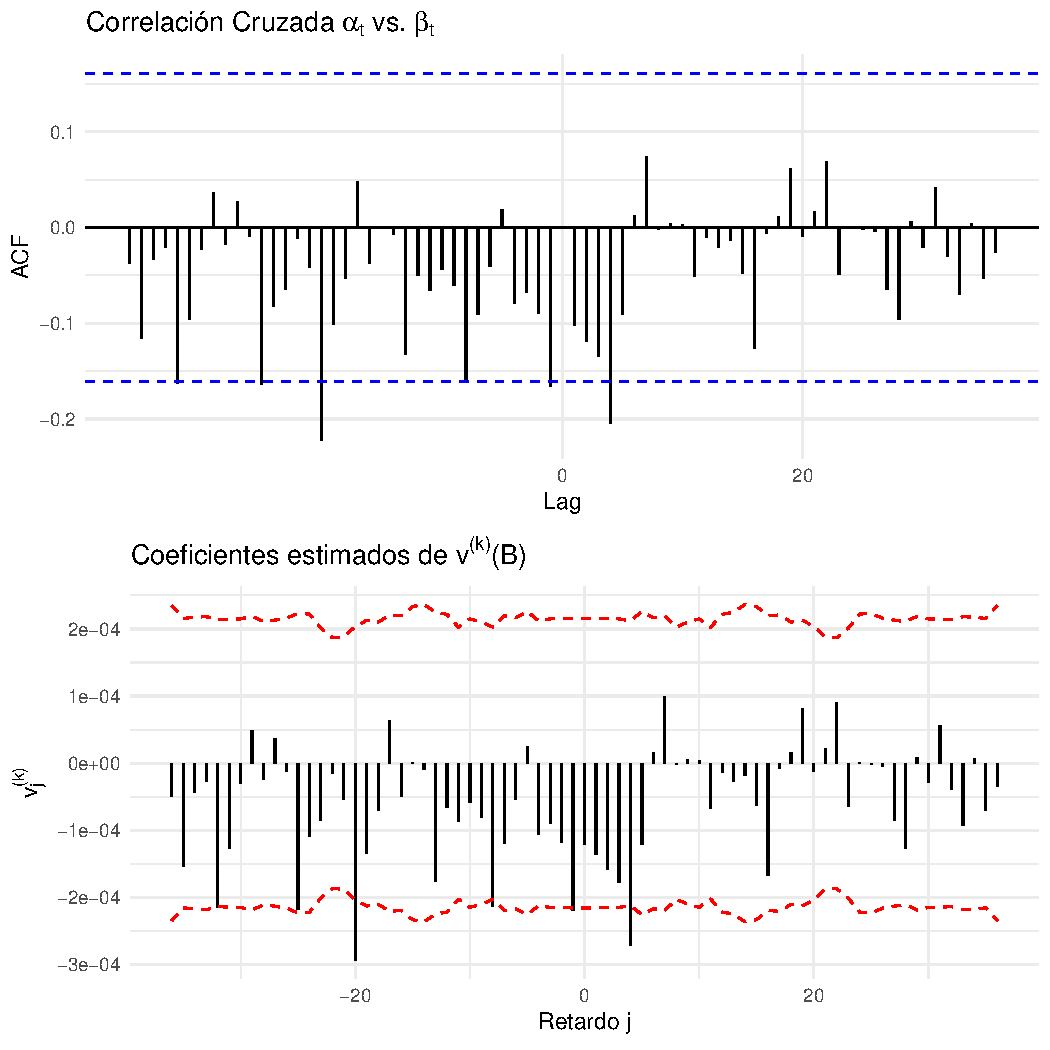
\includegraphics[width=\maxwidth]{figure/unnamed-chunk-43-1} 

}

\caption{\label{fig:vj3} Coeficientes $v_j$ estimados - Temperatura Mínima }\label{fig:unnamed-chunk-43}
\end{figure}


\end{knitrout}



\item Para la variable Humedad Relativa $x_t^{(4)}$, se observa que los coeficientes $\hat v_j^{(4)}$ se encuentran dentro de las bandas de confianza y no siguen un patrón en particular se toman $b=0$ y $m=0$ , a excepción de los retardos $j=3$ y $j=-7$ (figura \ref{fig:vj4}). Así, posibles valores a considerar son $n=3$ y $n=7$, pero por el principio de parsimonia, solo se considera $n=3$.



\begin{knitrout}
\definecolor{shadecolor}{rgb}{0.969, 0.969, 0.969}\color{fgcolor}\begin{figure}[H]

{\centering 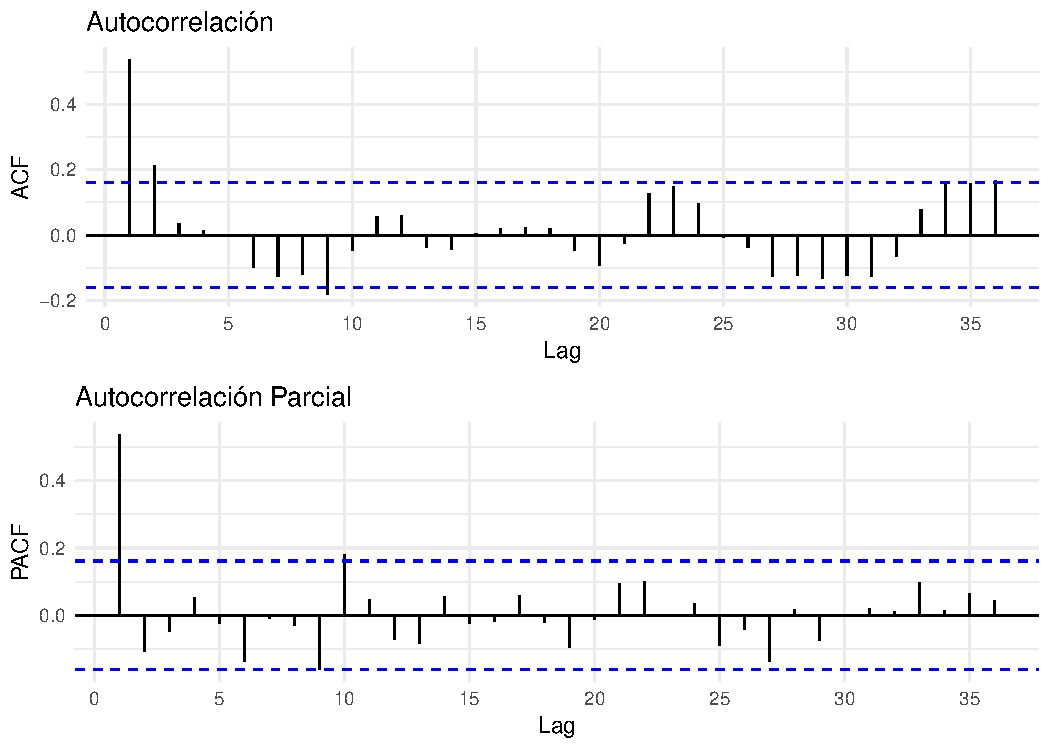
\includegraphics[width=\maxwidth]{figure/unnamed-chunk-44-1} 

}

\caption{\label{fig:vj4} Coeficientes $v_j$ estimados - Humedad Relativa }\label{fig:unnamed-chunk-44}
\end{figure}


\end{knitrout}



\end{enumerate}


Identificadas las funciones de respuesta al impulso, para cada una de las variables, considerando únicamente las variables que no se encuentren correlacionadas, 
%estimamos los coeficientes asociados, se muestran los coeficientes en la tabla $$ .
se continua con el paso 4 de la metodología, en este punto se debe identificar la estructura SARMA que compone el modelo SARIMAX, para ello, se consideran dos factores, el primero es que las funciones de respuesta al impulso $v^{(k)}(B)$ tienen como término común al polinomio estacional autoregresivo  (SAR) de grado 2, por lo que se incluye este en el modelo final. Otro factor a analizar es la perturbación $n_t$, para identificar si es necesario incluir más coeficientes tanto en la parte autoregresiva como media móvil del modelo final.

Para ello se procede a modelar $n_t$ precisamente mediante un modelo SARMA. Para este caso, la perturbación viene dada por:

$$n_t^{*} = y_t -  \alpha_t^{(1)}-\alpha_t^{(2)}-\alpha_t^{(3)}-\alpha_t^{(4)}$$

Observando la figura \ref{fig:acf_pertur} se ve que la función de autocorrelación y autocorrleación parcial de $n^{*}_t$ tienen picos fuera de las bandas de confianza en los retardos 1 y 10, en el resto de retardos muestra un comportamiento con picos periódicos, pero dentro de las bandas de confianza, por lo que podría ser necesario incluir polinomios estacionales en el modelo final. 

\begin{knitrout}
\definecolor{shadecolor}{rgb}{0.969, 0.969, 0.969}\color{fgcolor}\begin{figure}[H]

{\centering \includegraphics[width=\maxwidth]{figure/unnamed-chunk-45-1} 

}

\caption{\label{fig:acf_pertur} Autocorrelación $n_t$ }\label{fig:unnamed-chunk-45}
\end{figure}


\end{knitrout}


Tras analizar la función de autocorrelación de $n_t^{*}$, se propone el modelo ARMA$(1,0)$. Como se muestra en la tabla \ref{tab:arma_nt}, todos los coeficientes son significativos, mientras que analizando los residuos del modelo (ver figura \ref{fig:nt_resid}), se observa que todos los P-valores del estadístico Ljung-Box son mayores que 0.05, por lo tanto los residuos se comportan como un ruido blanco.


\begin{knitrout}
\definecolor{shadecolor}{rgb}{0.969, 0.969, 0.969}\color{fgcolor}\begin{table}

\caption{\label{tab:unnamed-chunk-46}\label{tab:arma_nt}Modelo ARMA(1,0) - Perturbación}
\centering
\begin{threeparttable}
\begin{tabular}[t]{lrrrrl}
\toprule
Coef & Estimate & Std.Error & z-value & Pr(>|z|) & Signif\\
\midrule
\rowcolor{gray!6}  ar1 & 0.534 & 0.0691 & 7.730 & 0 & ***\\
intercept & 794.235 & 86.9489 & 9.134 & 0 & ***\\
\bottomrule
\end{tabular}
\begin{tablenotes}
\item \textit{Resumen:} 
\item sigma\textasciicircum{}2 = 246784.96, loglikelihood = -1128.97, AIC = 2263.95, BIC =2272.94, Hannan-Quinn =2268.09
\end{tablenotes}
\end{threeparttable}
\end{table}


\end{knitrout}


\begin{knitrout}
\definecolor{shadecolor}{rgb}{0.969, 0.969, 0.969}\color{fgcolor}\begin{figure}[H]

{\centering \includegraphics[width=\maxwidth]{figure/unnamed-chunk-47-1} 

}

\caption{\label{fig:nt_resid} Residuos - Test Portmanteau (Ljung-Box) ARMA(1,0)}\label{fig:unnamed-chunk-47}
\end{figure}


\end{knitrout}


%%%%%%%%%%%%%%%%%%%%%%%%%%%%%%%


\subsubsection{Estimación del modelo}




A partir de las anteriores etapas, se identifica un modelo inicial del tipo SARIMAX $(1,0,0)(2,1,0)_{12}$ con 4 variables exógenas, y con funciones de respuesta al impulso con órdenes $(b_k,m_k,n_k)$ como se muestran a continuación:







\begin{itemize}
\item Precipitación $v^{(1)}$ : $b_1= 0$, $m_1=2$, $n_1=8$
\item Temperatura Máxima $v^{(2)}$ : $b_2= 0$, $m_2=0$, $n_2=0$
\item Temperatura Mínima $v^{(3)}$ : $b_3= 0$, $m_3=0$, $n_3=4$
\item Humedad Relativa $v^{(4)}$ : $b_4= 0$, $m_4=0$, $n_4=3$
\end{itemize}


Estimando los coeficientes de este modelo se obtienen los resultados de la tabla \ref{tab:sarimax_estim1}.

\begin{knitrout}
\definecolor{shadecolor}{rgb}{0.969, 0.969, 0.969}\color{fgcolor}\begin{table}

\caption{\label{tab:unnamed-chunk-51}\label{tab:sarimax_estim1}Modelo SARIMAX$(1,0,0)(2,1,0)$}
\centering
\begin{threeparttable}
\begin{tabular}[t]{lrrrrl}
\toprule
Coef & Estimate & Std.Error & z-value & Pr(>|z|) & Signif\\
\midrule
\rowcolor{gray!6}  ar1 & 0.5313 & 0.0769 & 6.9068 & 0.0000 & ***\\
sar1 & -0.5047 & 0.1022 & -4.9375 & 0.0000 & ***\\
\rowcolor{gray!6}  sar2 & 0.0073 & 0.1103 & 0.0664 & 0.9470 & \\
Precipitacion-AR1 & 0.0014 & 0.0995 & 0.0139 & 0.9889 & \\
\rowcolor{gray!6}  Precipitacion-AR2 & 0.0004 & NaN & NaN & NaN & NA\\
\addlinespace
Precipitacion-AR3 & -0.0015 & NaN & NaN & NaN & NA\\
\rowcolor{gray!6}  Precipitacion-AR4 & 0.0004 & 0.2781 & 0.0013 & 0.9990 & \\
Precipitacion-AR5 & 0.0039 & 0.1381 & 0.0279 & 0.9777 & \\
\rowcolor{gray!6}  Precipitacion-AR6 & 0.0075 & NaN & NaN & NaN & NA\\
Precipitacion-AR7 & -0.0108 & NaN & NaN & NaN & NA\\
\addlinespace
\rowcolor{gray!6}  Precipitacion-AR8 & -0.0197 & NaN & NaN & NaN & NA\\
Precipitacion-MA0 & -0.0759 & 0.6072 & -0.1251 & 0.9005 & \\
\rowcolor{gray!6}  Precipitacion-MA1 & -0.2714 & 0.1537 & -1.7652 & 0.0775 & .\\
Precipitacion-MA2 & -0.2411 & NaN & NaN & NaN & NA\\
\rowcolor{gray!6}  TemperaturaMax-MA0 & -2.6956 & 17.2030 & -0.1567 & 0.8755 & \\
\addlinespace
TemperaturaMin-AR1 & 0.1600 & NaN & NaN & NaN & NA\\
\rowcolor{gray!6}  TemperaturaMin-AR2 & 1.2014 & 0.0717 & 16.7484 & 0.0000 & ***\\
TemperaturaMin-AR3 & -0.4237 & 0.1022 & -4.1453 & 0.0000 & ***\\
\rowcolor{gray!6}  TemperaturaMin-AR4 & -0.5483 & 0.0225 & -24.3311 & 0.0000 & ***\\
TemperaturaMin-MA0 & -7.9281 & NaN & NaN & NaN & NA\\
\addlinespace
\rowcolor{gray!6}  HumedadRelativa-AR1 & -0.4741 & 0.1337 & -3.5447 & 0.0004 & ***\\
HumedadRelativa-AR2 & 0.5896 & 0.3065 & 1.9236 & 0.0544 & .\\
\rowcolor{gray!6}  HumedadRelativa-AR3 & 0.6813 & 0.0604 & 11.2786 & 0.0000 & ***\\
HumedadRelativa-MA0 & -4.7599 & 4.9517 & -0.9613 & 0.3364 & \\
\bottomrule
\end{tabular}
\begin{tablenotes}
\item \textit{Resumen:} 
\item sigma\textasciicircum{}2 = 313747.19, loglikelihood = -1040.07, AIC = 2130.15, BIC =2205.08, Hannan-Quinn =2164.61
\end{tablenotes}
\end{threeparttable}
\end{table}


\end{knitrout}





%%%%%%%%%%%%%%%%%%%%%%%%   QUITAR VARIABLES CORRELACIONADAS   %%%%%%%%%%%%%%%%%%%%%%%


\paragraph{Observación.} Como se ve en la tabla \ref{tab:sarimax_estim1} tiene varios de lo coeficientes no significativos, para varios de ellos no es posible estimar numéricamente sus errores estándar, por lo que es necesario, por una parte, quitar aquellas componentes menos significativas.  En esta etapa se hace notoria la necesidad de eliminar variables del modelo, para ello se considera el criterio de quitar aquellas variables exógenas que se encuentren correlacionadas entre si y que no tengan una alta correlación con la variable \textit{output} (Caudal). Para ello se observaron las funciones de correlación cruzada representadas en las figuras \ref{fig:cc_exogenas} y \ref{fig:cc_output} respectivamente.



%%%%%%%%%%%%%%%%%%%%%%%%%%%%%%%%%%%%%%%%%%%%%%%%%%%%%%%%%%%%%%%%%%%%%%%%%%%%%%%%%%%%%

Quitando la variable Temperatura Máxima y posteriormente Mínima, ya que tampoco tenía coeficientes asociados significativos, se llega al modelo SARIMAX $(1,0,0)(2,1,0)_{12}$, con 3 variables exógenas, cuyas funciones de respuesta al impulso tienen órdenes $(b_k,m_k,n_k)$ como se muestran a continuación:







\begin{itemize}
\item Precipitación $v^{(1)}$ : $b_1= 0$, $m_1=0$, $n_1=8$
% \item Temperatura Máxima $v^{(2)}$ : $b_2= 0, $m_2=tma2$, $n_2=tar2$
% \item Temperatura Mínima $v^{(3)}$ : $b_3= 0, $m_3=tma3$, $n_3=tar3$
\item Humedad Relativa $v^{(4)}$ : $b_4= 0$, $m_4=0$, $n_4=3$
\end{itemize}


Estimando los coeficientes de este modelo se obtienen los resultados de la tabla \ref{tab:sarimax_estim2}. Como se puede observar, para este modelo se obtiene que todos los coeficientes son significativos. 


\begin{knitrout}
\definecolor{shadecolor}{rgb}{0.969, 0.969, 0.969}\color{fgcolor}\begin{table}

\caption{\label{tab:unnamed-chunk-53}\label{tab:sarimax_estim2}Modelo SARIMAX$(1,0,0)(2,1,0)$}
\centering
\begin{threeparttable}
\begin{tabular}[t]{lrrrrl}
\toprule
Coef & Estimate & Std.Error & z-value & Pr(>|z|) & Signif\\
\midrule
\rowcolor{gray!6}  ar1 & 0.4786 & 0.0765 & 6.260 & 0e+00 & ***\\
sar1 & -0.6467 & 0.0894 & -7.235 & 0e+00 & ***\\
\rowcolor{gray!6}  sar2 & -0.3157 & 0.0898 & -3.515 & 4e-04 & ***\\
Precipitacion-AR1 & -0.3706 & 0.0728 & -5.090 & 0e+00 & ***\\
\rowcolor{gray!6}  Precipitacion-AR2 & -0.4814 & 0.0641 & -7.513 & 0e+00 & ***\\
\addlinespace
Precipitacion-AR3 & -0.4302 & 0.0738 & -5.832 & 0e+00 & ***\\
\rowcolor{gray!6}  Precipitacion-AR4 & -0.4701 & 0.0800 & -5.873 & 0e+00 & ***\\
Precipitacion-AR5 & -0.4877 & 0.0736 & -6.625 & 0e+00 & ***\\
\rowcolor{gray!6}  Precipitacion-AR6 & -0.3947 & 0.0790 & -4.998 & 0e+00 & ***\\
Precipitacion-AR7 & -0.4521 & 0.0776 & -5.824 & 0e+00 & ***\\
\addlinespace
\rowcolor{gray!6}  Precipitacion-AR8 & -0.8195 & 0.0973 & -8.423 & 0e+00 & ***\\
Precipitacion-MA0 & 1.1374 & 0.3457 & 3.291 & 1e-03 & ***\\
\rowcolor{gray!6}  HumedadRelativa-AR1 & 0.7383 & 0.0825 & 8.951 & 0e+00 & ***\\
HumedadRelativa-AR2 & 0.7195 & 0.1122 & 6.415 & 0e+00 & ***\\
\rowcolor{gray!6}  HumedadRelativa-AR3 & -0.8279 & 0.0864 & -9.581 & 0e+00 & ***\\
\addlinespace
HumedadRelativa-MA0 & -11.6721 & 3.3004 & -3.537 & 4e-04 & ***\\
\bottomrule
\end{tabular}
\begin{tablenotes}
\item \textit{Resumen:} 
\item sigma\textasciicircum{}2 = 216121.53, loglikelihood = -1031.31, AIC = 2096.62, BIC =2147.57, Hannan-Quinn =2120.05
\end{tablenotes}
\end{threeparttable}
\end{table}


\end{knitrout}

Sin embargo, al analizar sus residuos (ver figura \ref{fig:sarima_estim2}), se ve que los P-valores del estadístico de Ljung-Box son menores a 0.05, por lo tanto se considera que la autocorrelación de los residuos es significativa, y se rechaza su independencia.

\begin{knitrout}
\definecolor{shadecolor}{rgb}{0.969, 0.969, 0.969}\color{fgcolor}\begin{figure}[h]

{\centering \includegraphics[width=\maxwidth]{figure/unnamed-chunk-54-1} 

}

\caption{\label{fig:sarima_estim2} Residuos - Test Portmanteau (Ljung-Box) SARIMAX $(1,0,0)(2,1,0)_{12}$}\label{fig:unnamed-chunk-54}
\end{figure}


\end{knitrout}




%%%%%%%%%%%%%%%%%%%%%%%%%%%%%%%%%%%%%%%%%%%%%%%%%%%%%%%%%%%%%%%%%%%%%%%%%%%%%%%%%%


Tras probar varias combinaciones de parámetros y con la ayuda de las funciones de aucorrelación, se puede corregir las partes SARMA del modelo,y de las funciones de correlación cruzada entre los residuos y $x_t^{k}$ para corregir las funciones de respuesta al impulso, se llega al modelo SARIMAX $(1,0,0)(2,1,0)_{12}$, cuyas funciones de respuesta al impulso tienen órdenes $(b_k,m_k,n_k)$ como se muestran a continuación:








\begin{itemize}
\item Precipitación $v^{(1)}$ : $b_1= 0$, $m_1=0$, $n_1=2$
% \item Temperatura Máxima $v^{(2)}$ : $b_2= 0, $m_2=tma2$, $n_2=tar2$
% \item Temperatura Mínima $v^{(3)}$ : $b_3= 0, $m_3=tma3$, $n_3=tar3$
\item Humedad Relativa $v^{(4)}$ : $b_4= 0$, $m_4=0$, $n_4=2$
\end{itemize}


Estimando los coeficientes de este modelo se obtienen los resultados de la tabla \ref{tab:sarimax_estim3}. Como se puede observar, para este modelo se tienen todos los coeficientes significativos. 


\begin{knitrout}
\definecolor{shadecolor}{rgb}{0.969, 0.969, 0.969}\color{fgcolor}\begin{table}

\caption{\label{tab:unnamed-chunk-56}\label{tab:sarimax_estim3}Modelo SARIMAX$(1,0,0)(2,1,0)$}
\centering
\begin{threeparttable}
\begin{tabular}[t]{lrrrrl}
\toprule
Coef & Estimate & Std.Error & z-value & Pr(>|z|) & Signif\\
\midrule
\rowcolor{gray!6}  ar1 & 0.5542 & 0.0746 & 7.428 & 0.0000 & ***\\
sar1 & -0.7186 & 0.0860 & -8.360 & 0.0000 & ***\\
\rowcolor{gray!6}  sar2 & -0.3867 & 0.0843 & -4.585 & 0.0000 & ***\\
Precipitacion-AR1 & -1.7641 & 0.0529 & -33.338 & 0.0000 & ***\\
\rowcolor{gray!6}  Precipitacion-AR2 & -0.9481 & 0.0494 & -19.174 & 0.0000 & ***\\
\addlinespace
Precipitacion-MA0 & 0.1475 & 0.0882 & 1.673 & 0.0943 & .\\
\rowcolor{gray!6}  HumedadRelativa-AR2 & 0.7495 & 0.2187 & 3.428 & 0.0006 & ***\\
HumedadRelativa-MA0 & -7.3258 & 4.3291 & -1.692 & 0.0906 & .\\
\bottomrule
\end{tabular}
\begin{tablenotes}
\item \textit{Resumen:} 
\item sigma\textasciicircum{}2 = 254742.56, loglikelihood = -1043.44, AIC = 2104.89, BIC =2131.86, Hannan-Quinn =2117.29
\end{tablenotes}
\end{threeparttable}
\end{table}


\end{knitrout}



Y tras analizar los residuos asociados a este modelo (ver figura \ref{fig:sarimax_estim3}), se tiene que los P-valores del estadístico de Ljung-Box son mayores que 0.05, por lo que se puede aceptar que sus residuos son independientes. Así, este es el modelo que representará el Clúster 1. Se puede representar este modelo mediante la siguiente ecuación:


\begin{eqnarray} \label{eq:sarimax}
\Delta_{12} Y_t = \frac{0.148 }{1+ 1.764B + 0.948B^2} \Delta_{12} X^{(1)}_t + \frac{-7.326 }{1 - 0.749B^2} \Delta_{12} X^{(4)}_t     \nonumber\\
+ \frac{1}{( 1 - 0.554 B )(1+ 0.719 B^{12} +0.387 B^{24} )  }\varepsilon_t                  \label{prime}
\end{eqnarray}


\begin{knitrout}
\definecolor{shadecolor}{rgb}{0.969, 0.969, 0.969}\color{fgcolor}\begin{figure}[h]

{\centering \includegraphics[width=\maxwidth]{figure/unnamed-chunk-57-1} 

}

\caption{\label{fig:sarimax_estim3} Residuos - Test Portmanteau (Ljung-Box) SARIMAX $(1,0,0)(2,1,0)_{12}$}\label{fig:unnamed-chunk-57}
\end{figure}


\end{knitrout}



En la siguiente sección se hace una breve reseña del uso de la aplicación web creada para facilitar la ejecución de la metodología ya descrita.

Mientras que en la sección (\autoref{chap:resultados}) se muestran a detalle los resultados de modelar todas las series que componen el clúster 1, partiendo de un modelo con los mismos parámetros (aunque no los mismos coeficientes), así mismo se muestran las predicciones e intervalos de confianza obtenidas de los modelos SARIMA y SARIMAX correspondientes.














%%%%%%%%%%%%%%%%%%%%%%%%%%%%%%%%%%%%%%%%%%%%%%%%%%%%%%%%%%%%%%%%%%%%%%%%%%%%%%%%%%%%%




%Capitulo3: Aplicacion Web  .............................

\chapter{Aplicación Web}
\label{chp:webapp}

A continuación, se muestra una guía de uso de la aplicación web que implementa la metodología antes descrita.


\section{Módulo: Clustering}

En este módulo el usuario puede realizar una serie de variantes del análisis clúster expuesto en este documento. Incorporta 10 métricas distintas como:

\begin{enumerate}
\item Autocorrelación
\item Correlación de Pearson
\item Correlación Temporal
\item Métrica Euclidea
\item Métrica de Fourier
\item Métrica Infinito
\item Métrica Manhatan
\item Métrica Minkwoski
\item Autocorrelación Parcial
\item Periodograma
\end{enumerate}


Así mismo es posible usar 3 diferentes algoritmos de agrupamiento:

\begin{enumerate}
\item K-Medias
\item PAM - CLARA
\item Clúster Jerárquico
\end{enumerate}

Como se ilustra  en la figura (\ref{fig:app_clustering}), una vez definidos estos dos parámetros y el número de clústers que se desean construir, y dando clic en el botón \texttt{Clusterizar}, la aplicación web crea los clústers, además una sugerencia del número óptimo de clústers que se deben construir, también se muestran las estaciones georeferenciadas en un mapa, opcionalmente su representación MDS en $\mathbb{R}^2$, así mismo se genera una tabla con las estaciones y a que clúster corresponden, si se seleccionan estaciones de esta lista, la aplicación muestra gráficos de las series de tiempo de Caudales asociados a estas estaciones. 


\begin{figure}[h]
\caption{Módulo Clustering}
\includegraphics[width=15cm]{Cap3-WebApp/modulo_clustering}
\label{fig:app_clustering}
\centering
\end{figure}


\section{Módulo: SARIMAX}

Este módulo se compone de dos secciones, la primera (ver \ref{fig:modulo_sarimax2}) busca definir las componentes SARIMA del modelo asociado al Caudal de una estación (de un clúster predefinido), en nuestro caso, la estación \textit{medoide} o central del clúster, aunque se puede elegir cualquiera. En la segunda parte se trata de elegir las variables regresoras asociadas a estaciones de medición climatologica (ver \ref{fig:modulo_sarimax3}). Elegidas estas dos componentes, la aplicación estima el modelo asociado y muestra una serie de estadísticos de validación del modelo, análisis de residuos, predicciones del modelo (para la serie modelada), y una tabla con todos los modelos estimados para los caudales del clúster (ver \ref{fig:modulo_sarimax5}).


\begin{figure}[h]
\caption{Módulo SARIMAX}
\includegraphics[width=15cm]{Cap3-WebApp/modulo_sarimax1}
\label{fig:modulo_sarimax1}
\centering
\end{figure}

\begin{figure}[h]
\caption{Módulo SARIMAX}
\includegraphics[width=15cm]{Cap3-WebApp/modulo_sarimax2}
\label{fig:modulo_sarimax2}
\centering
\end{figure}

\begin{figure}[h]
\caption{Módulo SARIMAX}
\includegraphics[width=15cm]{Cap3-WebApp/modulo_sarimax3}
\label{fig:modulo_sarimax3}
\centering
\end{figure}

\begin{figure}[h]
\caption{Módulo SARIMAX}
\includegraphics[width=15cm]{Cap3-WebApp/modulo_sarimax4}
\label{fig:modulo_sarimax4}
\centering
\end{figure}

\begin{figure}[h]
\caption{Módulo SARIMAX}
\includegraphics[width=15cm]{Cap3-WebApp/modulo_sarimax5}
\label{fig:modulo_sarimax5}
\centering
\end{figure}

\begin{figure}[h]
\caption{Módulo SARIMAX}
\includegraphics[width=15cm]{Cap3-WebApp/modulo_sarimax6}
\label{fig:modulo_sarimax6}
\centering
\end{figure}




%Conclusiones y Recomendaciones  .....................

\chapter{Resultados}
\label{chap:resultados}

En el presente capítulo se analizan los modelos SARIMA (ver \ref{eq:sarima}) y SARIMAX (ver \ref{eq:sarimax}) estimados para cada una de las series de tiempo asociadas a Caudales medidos en las estaciones que componen el clúster 1. 



Para el caso del modelo SARIMA$(4,0,0)(1,1,0)_{12}$, se resumen en la tabla \ref{tab:sarima1_resumen}, los coeficientes estimados, su significancia, varianza de los residuos, y estadísticos como AIC,BIC, de cada una de las 41 series que componen el clúster 1. Como se puede observar los coeficientes asociados al retardo 1 de los polinomios autoregresivo y autoregresivo estacional, son significativos en las 41 estaciones, mientras que los coeficientes asociados a los retardos 2 y 3 del polinomio autoregresivo son significativos en únicamente cinco estaciones. En cambio el coeficiente asociado al retardo 4 del polinomio autoregresivo es no significativo en todos los casos.









\begin{knitrout}
\definecolor{shadecolor}{rgb}{0.969, 0.969, 0.969}\color{fgcolor}\begin{table}

\caption{\label{tab:unnamed-chunk-60}\label{tab:sarima1_resumen}Modelo SARIMA$(4,0,0)(1,1,0)_{12}$ - Clúster 1}
\centering
\resizebox{\linewidth}{!}{
\begin{tabular}[t]{llllllrrrr}
\toprule
Estación-Caudal & ar1 & ar2 & ar3 & ar4 & sar1 & sigma^2 & Log-Verosim & AIC & BIC\\
\midrule
\rowcolor{gray!6}  LAJES/P.PASSOS/FONTES NOVA (202) & 0.399 *** & 0.087 & 0.057 & 0.021 & -0.384 *** & 1.155e+01 & -360.5 & 733.0 & 750.4\\
14 DE JULHO (284) & 0.36 *** & 0.067 & -0.082 & 0.125 & -0.569 *** & 6.655e+04 & -950.6 & 1913.2 & 1930.7\\
\rowcolor{gray!6}  CASTRO ALVES (98) & 0.315 *** & 0.092 & -0.094 & 0.131 & -0.573 *** & 2.125e+04 & -873.0 & 1758.0 & 1775.5\\
BAIXO IGUAÇU (81) & 0.586 *** & -0.173 . & 0.027 & -0.044 & -0.424 *** & 1.367e+06 & -1155.1 & 2322.1 & 2339.6\\
\rowcolor{gray!6}  BARRA GRANDE (215) & 0.423 *** & 0.03 & -0.049 & 0.099 & -0.538 *** & 5.915e+04 & -942.3 & 1896.6 & 1914.1\\
\addlinespace
CAMPOS NOVOS (216) & 0.551 *** & -0.101 & 0.029 & 0.05 & -0.524 *** & 7.836e+04 & -961.4 & 1934.7 & 1952.2\\
\rowcolor{gray!6}  DESVIO JORDÃO ARTIFICIAL (70) & 0.226 ** & -0.133 & 0.091 & -0.076 & -0.503 *** & 4.526e+03 & -767.2 & 1546.3 & 1563.8\\
GARIBALDI (89) & 0.551 *** & -0.103 & 0.032 & 0.05 & -0.526 *** & 6.388e+04 & -947.5 & 1907.0 & 1924.5\\
\rowcolor{gray!6}  MACHADINHO (217) & 0.592 *** & -0.122 & 0.031 & 0.072 & -0.531 *** & 3.140e+05 & -1055.8 & 2123.7 & 2141.2\\
PEDREIRA (109) & 0.229 ** & 0.08 & 0.252 ** & 0.064 & -0.532 *** & 7.163e+01 & -485.6 & 983.2 & 1000.7\\
\addlinespace
\rowcolor{gray!6}  PIMENTAL ARTIFICIAL (302) & 0.295 *** & -0.225 * & 0.098 & -0.05 & -0.511 *** & 2.369e+06 & -1193.0 & 2397.9 & 2415.4\\
SÃO ROQUE (88) & 0.539 *** & -0.102 & 0.051 & 0.046 & -0.531 *** & 4.350e+04 & -921.4 & 1854.8 & 1872.3\\
\rowcolor{gray!6}  TRAIÇÃO (104) & 0.29 *** & 0.066 & 0.236 ** & 0.065 & -0.524 *** & 1.955e+02 & -553.8 & 1119.6 & 1137.1\\
SEGREDO Y DESVIO ARTIFICIAL (75) & 0.641 *** & -0.166 & -0.009 & -0.025 & -0.421 *** & 3.925e+05 & -1070.2 & 2152.4 & 2169.9\\
\rowcolor{gray!6}  ITÁ (92) & 0.54 *** & -0.096 & 0.047 & 0.059 & -0.534 *** & 6.723e+05 & -1107.6 & 2227.2 & 2244.7\\
\addlinespace
MONJOLINHO (220) & 0.467 *** & -0.014 & 0.123 & -0.009 & -0.516 *** & 5.723e+03 & -783.3 & 1578.7 & 1596.2\\
\rowcolor{gray!6}  PASSO FUNDO (93) & 0.529 *** & -0.04 & 0.096 & -0.011 & -0.508 *** & 1.593e+03 & -696.4 & 1404.7 & 1422.2\\
QUEBRA QUEIXO (286) & 0.47 *** & -0.029 & -0.028 & 0.03 & -0.454 *** & 4.057e+03 & -759.4 & 1530.8 & 1548.3\\
\rowcolor{gray!6}  SALTO OSORIO (78) & 0.61 *** & -0.177 . & 0.016 & -0.04 & -0.415 *** & 6.763e+05 & -1107.2 & 2226.3 & 2243.8\\
SALTO SANTIAGO (77) & 0.615 *** & -0.181 . & 0.019 & -0.042 & -0.417 *** & 6.109e+05 & -1100.3 & 2212.5 & 2230.0\\
\addlinespace
\rowcolor{gray!6}  SEGREDO (76) & 0.626 *** & -0.167 & -0.006 & -0.023 & -0.422 *** & 3.412e+05 & -1060.7 & 2133.4 & 2150.8\\
JACUÍ (112) & 0.536 *** & 0.083 & -0.045 & 0.107 & -0.504 *** & 2.097e+04 & -871.6 & 1755.3 & 1772.7\\
\rowcolor{gray!6}  PASSO REAL (111) & 0.536 *** & 0.083 & -0.045 & 0.108 & -0.505 *** & 2.055e+04 & -870.2 & 1752.5 & 1770.0\\
PEDRA DO CAVALO (254) & 0.293 *** & -0.114 & -0.092 & 0.129 & -0.701 *** & 8.109e+03 & -809.2 & 1630.4 & 1647.8\\
\rowcolor{gray!6}  ALTO TIETÊ (160) & 0.385 *** & 0.036 & 0.282 ** & 0.02 & -0.598 *** & 1.026e+01 & -354.2 & 720.3 & 737.8\\
\addlinespace
FOZ DO CHAPECÓ (94) & 0.535 *** & -0.064 & 0.036 & 0.053 & -0.541 *** & 1.023e+06 & -1136.2 & 2284.5 & 2302.0\\
\rowcolor{gray!6}  SALTO CAXIAS (222) & 0.586 *** & -0.173 . & 0.027 & -0.044 & -0.424 *** & 1.171e+06 & -1144.5 & 2301.0 & 2318.5\\
FOZ DO AREIA (74) & 0.614 *** & -0.137 & -0.028 & -0.018 & -0.43 *** & 2.532e+05 & -1040.5 & 2092.9 & 2110.4\\
\rowcolor{gray!6}  DESVIO JORDAO (73) & 0.548 *** & -0.143 & 0.057 & -0.086 & -0.445 *** & 1.102e+04 & -827.4 & 1666.8 & 1684.2\\
FUNDÃO (72) & 0.51 *** & -0.102 & 0.037 & -0.091 & -0.44 *** & 8.156e+03 & -806.9 & 1625.7 & 1643.2\\
\addlinespace
\rowcolor{gray!6}  MAUÁ (57) & 0.583 *** & -0.105 & 0.069 & -0.083 & -0.5 *** & 3.649e+04 & -909.2 & 1830.5 & 1847.9\\
MONTE CLARO (97) & 0.353 *** & 0.072 & -0.083 & 0.124 & -0.566 *** & 6.189e+04 & -945.6 & 1903.3 & 1920.8\\
\rowcolor{gray!6}  DONA FRANCISCA (114) & 0.443 *** & 0.218 * & -0.078 & 0.067 & -0.512 *** & 5.928e+04 & -942.3 & 1896.7 & 1914.2\\
ITAUBA (113) & 0.486 *** & 0.156 . & -0.067 & 0.098 & -0.508 *** & 3.651e+04 & -909.3 & 1830.7 & 1848.2\\
\rowcolor{gray!6}  PASSO SÃO JOÃO (103) & 0.523 *** & 0.129 & -0.022 & 0.048 & -0.483 *** & 4.345e+04 & -921.0 & 1854.0 & 1871.5\\
\addlinespace
SÃO JOSÉ (102) & 0.52 *** & 0.129 & -0.022 & 0.049 & -0.484 *** & 4.053e+04 & -916.3 & 1844.5 & 1862.0\\
\rowcolor{gray!6}  SANTA CLARA MG (283) & 0.453 *** & -0.096 & 0.113 & -0.002 & -0.465 *** & 4.825e+03 & -771.3 & 1554.6 & 1572.1\\
SANTA CLARA PR (71) & 0.5 *** & -0.089 & 0.031 & -0.092 & -0.441 *** & 7.481e+03 & -801.0 & 1614.0 & 1631.5\\
\rowcolor{gray!6}  BILLINGS (118) & 0.229 ** & 0.08 & 0.252 ** & 0.064 & -0.532 *** & 7.163e+01 & -485.6 & 983.2 & 1000.7\\
BILLINGS+PEDRAS (119) & 0.24 ** & 0.078 & 0.244 ** & 0.063 & -0.536 *** & 1.093e+02 & -514.4 & 1040.7 & 1058.2\\
\addlinespace
\rowcolor{gray!6}  PEDRAS (116) & 0.281 ** & 0.068 & 0.21 * & 0.058 & -0.549 *** & 4.100e+00 & -291.1 & 594.3 & 611.8\\
\bottomrule
\end{tabular}}
\end{table}


\end{knitrout}



En cuanto al modelo SARIMAX $(1,0,0)(2,1,0)_{12}$ con funciones de respuesta al impulso con órdenes:

\begin{itemize}
\item Precipitación $v^{(1)}$ : $b_1= 0$, $m_1=0$, $n_1=2$
% \item Temperatura Máxima $v^{(2)}$ : $b_2= 0, $m_2=tma2$, $n_2=tar2$
% \item Temperatura Mínima $v^{(3)}$ : $b_3= 0, $m_3=tma3$, $n_3=tar3$
\item Humedad Relativa $v^{(4)}$ : $b_4= 0$, $m_4=0$, $n_4=2$
\end{itemize}

Observando el resumen de los resultados de este modelo en la tabla \ref{tab:sarimax1_resumen}, se ve que todos los coeficientes asociados a la estructura SARIMA del modelo son significativos en todas las series de tiempo del clúster. En la mayoría de series, los retardos 1 y 2 del polinomio autoregresivo asociado a la variable exógena Precipitación, son significativos, seguidos por el retardo 2 del polinomio autoregresivo asociado a la variable Humedad Relativa. Los coeficientes asociados a los polinomios media móvil de las dos variables exógenas, son no significativos en su mayoría.






\begin{knitrout}
\definecolor{shadecolor}{rgb}{0.969, 0.969, 0.969}\color{fgcolor}
\begin{landscape}\begin{table}

\caption{\label{tab:unnamed-chunk-62}\label{tab:sarimax1_resumen}Modelo SARIMAX$(1,0,0)(2,1,0)_{12}$ - Clúster 1}
\centering
\resizebox{\linewidth}{!}{
\begin{tabular}[t]{lllllllllrrrr}
\toprule
Estación-Caudal & ar1 & sar1 & sar2 & Precipitacion-AR1 & Precipitacion-AR2 & Precipitacion-MA0 & HumedadRelativa-AR2 & HumedadRelativa-MA0 & sigma^2 & Log-Verosim & AIC & BIC\\
\midrule
\rowcolor{gray!6}  LAJES/P.PASSOS/FONTES NOVA (202) & 0.393 *** & -0.523 *** & -0.293 ** & 0.382 & 0.399 & 0.011 * & 0.141 & -0.115 & 1.059e+01 & -355.7 & 729.4 & 756.3\\
14 DE JULHO (284) & 0.368 *** & -0.82 *** & -0.439 *** & 1.65 *** & -0.876 *** & -0.198 ** & -0.167 & 10.392 * & 4.884e+04 & -932.1 & 1882.2 & 1909.2\\
\rowcolor{gray!6}  CASTRO ALVES (98) & 0.459 *** & -0.858 *** & -0.461 *** & 0.078 & -0.883 *** & 0.202 ** & -0.914 *** & 1.626 & 1.556e+04 & -854.9 & 1727.7 & 1754.7\\
BAIXO IGUAÇU (81) & 0.501 *** & -0.694 *** & -0.524 *** & 0.737 & -0.73 *** & -0.538 & 0.651 *** & -7.434 & 1.023e+06 & -1139.4 & 2296.7 & 2323.7\\
\rowcolor{gray!6}  BARRA GRANDE (215) & 0.443 *** & -0.806 *** & -0.454 *** & 0.805 & -0.969 *** & -0.118 & 0.653 ** & -2.018 & 4.144e+04 & -921.0 & 1860.1 & 1887.1\\
\addlinespace
CAMPOS NOVOS (216) & 0.486 *** & -0.718 *** & -0.372 *** & -0.844 *** & -0.948 *** & 0.258 . & 0.62 ** & -3.549 & 6.371e+04 & -949.0 & 1916.1 & 1943.1\\
\rowcolor{gray!6}  DESVIO JORDÃO ARTIFICIAL (70) & 0.213 * & -0.645 *** & -0.352 *** & -0.336 & 0.465 & -0.073 . & -0.53 ** & 1.805 . & 3.864e+03 & -757.8 & 1533.6 & 1560.5\\
GARIBALDI (89) & 0.483 *** & -0.718 *** & -0.369 *** & -0.84 *** & -0.946 *** & 0.23 * & 0.632 *** & -3.19 & 5.206e+04 & -935.3 & 1888.6 & 1915.5\\
\rowcolor{gray!6}  MACHADINHO (217) & 0.518 *** & -0.755 *** & -0.406 *** & 0.882 *** & -0.904 *** & -0.595 ** & 0.687 *** & -4.045 & 2.411e+05 & -1040.1 & 2098.1 & 2125.1\\
PEDREIRA (109) & 0.322 *** & -0.65 *** & -0.329 *** & -0.385 & 0.553 . & -0.012 * & 0.352 & 0.172 & 6.656e+01 & -481.5 & 981.0 & 1008.0\\
\addlinespace
\rowcolor{gray!6}  PIMENTAL ARTIFICIAL (302) & 0.386 *** & -0.862 *** & -0.308 ** & 1.037 & -0.169 & 0.56 & 0.266 . & -21.902 & 2.180e+06 & -1190.1 & 2398.2 & 2425.2\\
SÃO ROQUE (88) & 0.471 *** & -0.726 *** & -0.379 *** & -0.836 *** & -0.939 *** & 0.197 * & 0.633 *** & -2.826 & 3.500e+04 & -908.4 & 1834.8 & 1861.8\\
\rowcolor{gray!6}  TRAIÇÃO (104) & 0.412 *** & -0.647 *** & -0.294 *** & -0.383 & 0.56 . & -0.016 * & -0.338 & 0.347 & 1.852e+02 & -550.9 & 1119.9 & 1146.9\\
SEGREDO Y DESVIO ARTIFICIAL (75) & 0.547 *** & -0.654 *** & -0.478 *** & 0.192 & -0.839 *** & 0.701 . & -0.909 & 0.078 & 3.052e+05 & -1056.3 & 2130.7 & 2157.6\\
\rowcolor{gray!6}  ITÁ (92) & 0.523 *** & -0.745 *** & -0.431 *** & -1.456 *** & -0.936 *** & 0.138 & -0.748 *** & 16.543 * & 5.273e+05 & -1093.4 & 2204.8 & 2231.8\\
\addlinespace
MONJOLINHO (220) & 0.55 *** & -0.736 *** & -0.455 *** & 0.186 ** & -0.873 *** & 0.084 * & 0.545 . & -0.94 & 4.214e+03 & -765.2 & 1548.5 & 1575.5\\
\rowcolor{gray!6}  PASSO FUNDO (93) & 0.58 *** & -0.685 *** & -0.411 *** & -1.252 *** & -0.886 *** & 0.013 & -0.724 *** & 0.516 & 1.258e+03 & -682.4 & 1382.7 & 1409.7\\
QUEBRA QUEIXO (286) & 0.475 *** & -0.641 *** & -0.445 *** & 0.115 & -0.907 *** & 0.066 . & -0.612 & 0.226 & 3.097e+03 & -743.7 & 1505.3 & 1532.3\\
\rowcolor{gray!6}  SALTO OSORIO (78) & 0.515 *** & -0.651 *** & -0.508 *** & 0.528 & -0.442 * & 0.719 & -0.675 * & 10.371 & 5.412e+05 & -1095.6 & 2209.3 & 2236.3\\
SALTO SANTIAGO (77) & 0.518 *** & -0.65 *** & -0.475 *** & 0.208 & -0.841 *** & 0.858 . & -0.844 & 0.742 & 4.738e+05 & -1086.2 & 2190.3 & 2217.3\\
\addlinespace
\rowcolor{gray!6}  SEGREDO (76) & 0.536 *** & -0.653 *** & -0.467 *** & 0.197 & -0.838 *** & 0.643 . & -0.808 & 0.691 & 2.689e+05 & -1047.6 & 2113.2 & 2140.1\\
JACUÍ (112) & 0.61 *** & -0.738 *** & -0.494 *** & 1.703 *** & -0.905 *** & -0.085 * & -0.754 *** & 2.325 * & 1.382e+04 & -846.5 & 1711.1 & 1738.0\\
\rowcolor{gray!6}  PASSO REAL (111) & 0.611 *** & -0.738 *** & -0.493 *** & 1.702 *** & -0.905 *** & -0.085 * & -0.753 *** & 2.298 * & 1.354e+04 & -845.2 & 1708.3 & 1735.3\\
PEDRA DO CAVALO (254) & 0.221 * & -0.831 *** & -0.228 * & 0.472 *** & -0.46 *** & 0.544 *** & -0.243 & -0.533 & 6.178e+03 & -790.9 & 1599.7 & 1626.7\\
\rowcolor{gray!6}  ALTO TIETÊ (160) & 0.441 *** & -0.736 *** & -0.316 *** & 0.095 & -0.079 & 0.007 * & 0.255 & 0.206 * & 8.810e+00 & -344.6 & 707.1 & 734.1\\
\addlinespace
FOZ DO CHAPECÓ (94) & 0.549 *** & -0.768 *** & -0.424 *** & 0.09 & 0.133 & -0.263 & 0.751 *** & -3.08 & 8.488e+05 & -1125.9 & 2269.8 & 2296.8\\
\rowcolor{gray!6}  SALTO CAXIAS (222) & 0.499 *** & -0.688 *** & -0.532 *** & -0.342 *** & -0.889 *** & -1.097 * & 0.503 * & -13.236 & 8.203e+05 & -1124.5 & 2266.9 & 2293.9\\
FOZ DO AREIA (74) & 0.488 *** & -0.666 *** & -0.439 *** & 0.083 & 0.739 *** & 0.613 . & 0.464 * & -16.179 . & 1.974e+05 & -1026.3 & 2070.5 & 2097.5\\
\rowcolor{gray!6}  DESVIO JORDAO (73) & 0.436 *** & -0.685 *** & -0.526 *** & -1.086 & -0.135 & 0.023 & 0.271 & -4.832 * & 7.909e+03 & -808.7 & 1635.3 & 1662.3\\
FUNDÃO (72) & 0.415 *** & -0.684 *** & -0.526 *** & -1.152 & -0.191 & 0.018 & 0.281 . & -4.058 * & 5.855e+03 & -788.2 & 1594.4 & 1621.4\\
\addlinespace
\rowcolor{gray!6}  MAUÁ (57) & 0.571 *** & -0.698 *** & -0.434 *** & -1.274 *** & -0.961 *** & 0.057 & -0.916 *** & 2.158 & 2.820e+04 & -894.1 & 1806.2 & 1833.2\\
MONTE CLARO (97) & 0.458 *** & -0.825 *** & -0.475 *** & -0.021 & -0.913 *** & 0.307 & -0.855 *** & 3.848 & 4.709e+04 & -930.1 & 1878.2 & 1905.2\\
\rowcolor{gray!6}  DONA FRANCISCA (114) & 0.594 *** & -0.747 *** & -0.517 *** & 0.202 * & -0.807 *** & 0.383 ** & 0.363 & -2.89 & 4.192e+04 & -922.4 & 1862.7 & 1889.7\\
ITAUBA (113) & 0.641 *** & -0.717 *** & -0.544 *** & 0.39 *** & -0.963 *** & 0.157 * & -0.901 *** & 2.882 * & 2.386e+04 & -884.3 & 1786.7 & 1813.7\\
\rowcolor{gray!6}  PASSO SÃO JOÃO (103) & 0.557 *** & -0.713 *** & -0.529 *** & 1.694 *** & -0.901 *** & -0.168 * & -0.796 *** & 2.458 & 2.712e+04 & -892.7 & 1803.4 & 1830.4\\
\addlinespace
SÃO JOSÉ (102) & 0.556 *** & -0.715 *** & -0.532 *** & 1.695 *** & -0.902 *** & -0.161 * & -0.796 *** & 2.337 & 2.519e+04 & -887.8 & 1793.5 & 1820.5\\
\rowcolor{gray!6}  SANTA CLARA MG (283) & 0.317 *** & -0.614 *** & -0.323 *** & 0.693 *** & -0.027 & 0.388 *** & 0.516 *** & -1.531 & 2.930e+03 & -738.6 & 1495.3 & 1522.3\\
SANTA CLARA PR (71) & 0.445 *** & -0.641 *** & -0.519 *** & 0.48 *** & -1.072 *** & 0.001 & 0.302 . & -3.758 . & 5.326e+03 & -781.5 & 1581.0 & 1608.0\\
\rowcolor{gray!6}  BILLINGS (118) & 0.164 . & -0.787 *** & -0.374 *** & 0.33 ** & 0.226 * & 0.057 *** & -0.312 & 0.268 . & 3.993e+01 & -447.9 & 913.8 & 940.8\\
BILLINGS+PEDRAS (119) & 0.173 * & -0.783 *** & -0.365 *** & 0.339 ** & 0.219 * & 0.07 *** & -0.299 & 0.342 * & 6.047e+01 & -476.1 & 970.1 & 997.1\\
\addlinespace
\rowcolor{gray!6}  PEDRAS (116) & 0.248 * & -0.766 *** & -0.338 *** & 0.223 & 0.141 & 0.014 *** & -0.327 & 0.042 & 2.310e+00 & -253.8 & 525.5 & 552.5\\
\bottomrule
\end{tabular}}
\end{table}
\end{landscape}


\end{knitrout}


Finalmente, analizando los estadísticos AIC, BIC, y $\hat\sigma^2$ de los dos modelo, se observa, en cada una de las estaciones, que estos criterios se minimizan al usar el modelo SARIMAX para modelar los caudales, así mismo, al analizar el logaritmo de la verosimilitud se ve que este se maximiza precisamente en el modelo SARIMAX, por esta razón, se elige este último como el modelo que representará el clúster y a partir del cual se puede realizar pronósticos. Esto ocurre en los 4 clústers, tal como se puede corroborar en los apéndices \ref{ap:sarima} y \ref{ap:sarimax}, en donde se puede observar una clara ventaja al usar los modelos SARIMAX en el modelamiento de caudales. Por ejemplo, para la serie de tiempo asociada a la estación \textit{14 DE JULHO (284)} considerando el modelo SARIMA, se obtiene un $AIC = 1913.2$, un $BIC=1930.7$, $\hat\sigma = 6655 $ y el Log-Verosimilitud $= -950.6$, mientras que para el modelo SARIMAX se obtiene un $AIC = 1882.2$, un $BIC=1909.2$, $\hat\sigma = 4884 $ y el Log-Verosimilitud $=-932.1$, es decir, el modelo SARIMAX es mejor en todos los criterios. Así mismo, si se analizan las predicciones producidas por los dos modelos (ver \ref{fig:predic14}), se ve que si bien los dos tienen predicciones (en azul) próximas a los valores reales de la serie (en rojo), el modelo SARIMAX produce predicciones más acertadas.


\begin{knitrout}
\definecolor{shadecolor}{rgb}{0.969, 0.969, 0.969}\color{fgcolor}\begin{figure}[h]

{\centering \includegraphics[width=\maxwidth]{figure/unnamed-chunk-63-1} 

}

\caption{\label{fig:predic14} Predicción de Modelos SARIMA y SARIMAX}\label{fig:unnamed-chunk-63}
\end{figure}


\end{knitrout}





\chapter{Conclusiones y Recomendaciones}



% Conclusion Objetivo General
% El objetivo del proyecto es utilizar el Análisis Clúster para agrupar estaciones (asociadas a ríos
% en Brasil), basándonos en el comportamiento temporal del caudal de los ríos que se mide en
% dichas estaciones, y posteriormente modelar los caudales (1 modelo por clúster) usando
% variables micro y macro climáticas.


En conclusión el uso de la metodología aquí planteada permite utilizar una variante del Análisis Clúster para modelar las 179 series de tiempo de caudales (asociadas a estaciones de medición en todo Brasil), a partir del modelamiento de 4 series de tiempo correspondientes a las \textit{medoides} de cada clúster, reduciendo así significativamente el tiempo de modelamiento que hubiera tomado hacerlo directamente.




% Conclusion Objetivo 1

% Comparar una gama de técnicas tanto de clusterización, así como la elección de
% distintas métricas o funciones de disimilitud a fin de identificar aquella combinación
% (disimilitud /algoritmo de clusterización) que permita un adecuado agrupamiento de las
% series de tiempo asociadas a los caudales de los principales ríos de Brasil, que tienen la
% peculiaridad de que dichas series son usualmente estacionales, y este tipo de series no
% han sido analizadas con esta técnica previamente.

Además se pudieron probar satisfactoriamente una variedad de algoritmos de clusterización así como distintas métricas (funciones de disimilitud) y elegir uno en base a su efectividad al momento de agrupar series de tiempo estacionales.


% Conclusion Objetivo 2

% Comparar el modelamiento de estas series de tiempo usando el análisis clúster versus el
% modelamiento sin un previo análisis, a fin de validar la metodología de clusterización
% planteada, y además mostrar posibles ventajas en cuanto a tiempo y eficiencia de la
% metodología planteada

En cuanto al modelamiento basado en la metodología Box y Jenkins se observó que si bien la correcta implementación del modelamiento SARIMAX supone un análisis más extenso, al considerar muchos más factores en su identificación, que el necesario para llevar a cabo el modelamiento SARIMA aquí propuesto, los modelos SARIMAX ofrecen mejores resultados, en términos de estadísticos de validación, criterios de información y también en predicción (en casi todos los casos). 


% Conclusion Objetivo 3


% Encontrar los factores macro y micro - climáticos determinantes del nivel de caudal para
% cada clúster y comparar como varían sus efectos entre uno clúster y otro.

Otro aporte importante del uso de modelos SARIMAX es que permitió identificar y medir la incidencia de factores climáticos a nivel local que interaccionan y afectan el comportamiento temporal de los caudales, factores como la precipitación, la humedad relativa y temperatura.
% Conclusion en terminos de POLITICAS
Conocido el comportamiento temporal de los caudales, a partir de las predicciones arrojadas por los modelos planteados, que podrían hacerse con una alta precisión para un horizonte de tiempo considerablemente grande (de varios años al futuro), dicho de otra manera, se puede calcular anticipadamente la oferta energética generada por el sector hidroeléctrico del país, que a la postre permitiría establecer una planificación del uso de energía hidroeléctrica  y también de energías alternativas (eólica, nuclear, solar) para cubrir la demanda interna y externa del país, ya que Brasil exporta energía eléctrica a países como Argentina.


% Coclucion 4

% 4. Automatizar la descomposición y Análisis Clúster de series de tiempo de Caudales a
% través de la utilización de software estadístico y programación.

Finalmente, la implementación y automatización de la metodología aquí propuesta que dieron paso a rutinas generales ejemplificadas en la Aplicación web creada para este estudio, dan muestra de la fácil reproducibilidad de esta metodología en una variedad de contextos distintos a los aquí abordados y abren la puerta a una variedad de análisis de datos de origen geográfico y temporal. 
% RECOMENDACIONES
Así mismo, cabe la posibilidad de extender este estudio a una escala mucho mayor ya sea considerando series de mayor frecuencia, o mayor cantidad de series, teniendo en cuenta algunas barreras en cuanto a la eficiencia de los algoritmos utilizados versus los recursos de hardware disponibles. A modo de ejemplo, en pruebas preliminares al desarrollo de este estudio, se consideraron series de frecuencia diaria, donde se encontraron cuellos de botella principalmente en el cálculo de la matriz de distancias (o disimilitudes) de la primera etapa, donde el tiempo de cálculo llegó a tomar un par de horas, en contraste con los tres minutos que tomó este proceso para series mensuales. Hay que notar que el tiempo de cálculo depende tanto del número de series de tiempo así como del número de observaciones que posee cada una, así, el tiempo de cálculo de la matriz crece al menos cuadráticamente cuando crecen estos dos factores. Por lo tanto, si el objetivo es escalar está metodología a un contexto por ejemplo de Big Data, es necesario considerar, por una parte, la necesidad de implementar algoritmos aún más eficientes que los expuestos aquí, por ejemplo, paralelizando el cálculo de la matriz de distancias, y también de la distancia persé, otra mejora posible es la de usar el algoritmo de agrupamiento CLARANS que es una extensión más eficiente del algoritmo CLARA. Por otro lado, hay que considerar el uso de otros recursos de hardware necesarios para dicha implementación, es decir, vía Computación distribuida o vía Computación de alto rendimiento (\textit{High performance Computing, HPC}).
%%% 


% Recomendaciones

% Además, cabe recalcar que está metodología, así planteada, es extensible una variedad de contextos, y a una escala mucho mayor, ya sea considerando series de mayor frecuencia, o mayor cantidad de series, teniendo en cuenta algunas barreras en cuanto a la eficiencia de los algoritmos utilizados versus los recursos de hardware disponibles. A modo de ejemplo, en pruebas preliminares al desarrollo de este estudio, se consideraron series de frecuencia diaria, donde se encontraron cuellos de botella principalmente en el cálculo de la matriz de distancias (o disimilitudes) de la primera etapa, donde el tiempo de cálculo llegó a tomar un par de horas, en contraste con los tres minutos que tomó este proceso para series mensuales. Hay que notar que el tiempo de cálculo depende tanto del número de series de tiempo así como del número de observaciones que posee cada una, así, el tiempo de cálculo de la matriz crece al menos cuadráticamente cuando crecen estos dos factores. Por lo tanto, si el objetivo es escalar está metodología a un contexto por ejemplo de Big Data, es necesario considerar, por una parte, la necesidad de implementar algoritmos aún más eficientes que los expuestos aquí, por ejemplo, paralelizando el cálculo de la matriz de distancias, y por otra, los recursos necesarios para dicha implementación, es decir, vía Computación distribuida o vía Computación de alto rendimiento (\textit{High performance Computing o HPC}).



















%%%%%%%%%%%%%%%%%%%%%%   APENDICES     %%%%%%%%%%%%%%%%%%%%%%%%%
\appendix


\chapter{Aplicación Web}
\label{apnd:webapp}

A continuación, mostramos la implementación en código R de la Aplicación Web desarrollada con el paquete \textit{Shiny}, \cite{shiny}, que contiene el análisis completo de las series de tiempo de flujos de rios de Brasil. Este aplicacion esta compuesta principalmente por tres archivos: \textit{global} , \textit{ui}  y \textit{server}, tal como puede ver en el mapa de archivos de la aplicación en la figura \ref{fig:mapa_webapp}.

\begin{figure}[h]
\caption{Estructura de la Aplicación Web}
\includegraphics[width=15cm]{MapaApp.eps}
\label{fig:mapa_webapp}
\centering
\end{figure}

\paragraph{Nota. } La aplicación Web con el análisis completo, se encuentra disponible para su uso en la siguiente dirección:
{\color{blue} https://cristianpachacama.shinyapps.io/TesisBorrrador/}.

Además puede encontrar el código fuente de la misma en el repositorio de GitHub:
{\color{blue} https://github.com/CristianPachacama/AppTesis/}


\section{Paquetes (global.R)}

Este archivo contiene la declaración de los paquetes extras, que contienen tods las funciones que se usaran en la aplicación web, y que son necesarios para su correcto funcionamiento.

\begin{knitrout}\footnotesize
\definecolor{shadecolor}{rgb}{0.969, 0.969, 0.969}\color{fgcolor}\begin{kframe}
\begin{alltt}
\hlcom{#!!!!!!!!!!!!!!!!!!!!!!!!!!!!!!!!!!!!!!!!!!!!!!!!!!!!!!!!!!!}
\hlcom{#------------------        global.R       ------------------}
\hlcom{#!!!!!!!!!!!!!!!!!!!!!!!!!!!!!!!!!!!!!!!!!!!!!!!!!!!!!!!!!!!}

\hlstd{pkgTest} \hlkwb{<-} \hlkwa{function}\hlstd{(}\hlkwc{x}\hlstd{)\{}
  \hlkwa{if} \hlstd{(}\hlopt{!}\hlkwd{require}\hlstd{(x,}\hlkwc{character.only} \hlstd{=} \hlnum{TRUE}\hlstd{))\{}
    \hlkwd{install.packages}\hlstd{(x,}\hlkwc{dep}\hlstd{=}\hlnum{TRUE}\hlstd{)}
    \hlkwa{if}\hlstd{(}\hlopt{!}\hlkwd{require}\hlstd{(x,}\hlkwc{character.only} \hlstd{=} \hlnum{TRUE}\hlstd{))} \hlkwd{stop}\hlstd{(}\hlstr{"Paquete no encontrado"}\hlstd{)}
  \hlstd{\}}
\hlstd{\}}
\hlcom{#Descarga de Paquetes ================================}
\hlkwd{pkgTest}\hlstd{(}\hlstr{"shinydashboard"}\hlstd{)}
\hlkwd{pkgTest}\hlstd{(}\hlstr{"ggplot2"}\hlstd{)}
\hlkwd{pkgTest}\hlstd{(}\hlstr{"dygraphs"}\hlstd{)}
\hlkwd{pkgTest}\hlstd{(}\hlstr{"TSstudio"}\hlstd{)}
\hlkwd{pkgTest}\hlstd{(}\hlstr{"leaflet"}\hlstd{)}
\hlkwd{pkgTest}\hlstd{(}\hlstr{"htmltools"}\hlstd{)}
\hlkwd{pkgTest}\hlstd{(}\hlstr{"rgdal"}\hlstd{)}
\hlkwd{pkgTest}\hlstd{(}\hlstr{"readr"}\hlstd{)}
\hlkwd{pkgTest}\hlstd{(}\hlstr{"DT"}\hlstd{)}
\hlkwd{pkgTest}\hlstd{(}\hlstr{"dplyr"}\hlstd{)}
\hlkwd{pkgTest}\hlstd{(}\hlstr{"reshape2"}\hlstd{)}
\hlkwd{pkgTest}\hlstd{(}\hlstr{"lmtest"}\hlstd{)}
\hlkwd{pkgTest}\hlstd{(}\hlstr{"TSdist"}\hlstd{)}
\hlkwd{pkgTest}\hlstd{(}\hlstr{"xts"}\hlstd{)}
\hlkwd{pkgTest}\hlstd{(}\hlstr{"stlplus"}\hlstd{)}
\hlkwd{pkgTest}\hlstd{(}\hlstr{"TSA"}\hlstd{)}
\hlkwd{pkgTest}\hlstd{(}\hlstr{"forecast"}\hlstd{)}
\hlkwd{pkgTest}\hlstd{(}\hlstr{"smacof"}\hlstd{)}
\hlkwd{pkgTest}\hlstd{(}\hlstr{"cluster"}\hlstd{)}
\hlkwd{pkgTest}\hlstd{(}\hlstr{"ks"}\hlstd{)}
\hlkwd{pkgTest}\hlstd{(}\hlstr{"fpca"}\hlstd{)}
\hlkwd{pkgTest}\hlstd{(}\hlstr{"fdapace"}\hlstd{)}

\hlcom{# Paquetes Necesarios ===============}
\hlkwd{library}\hlstd{(shiny)}
\hlkwd{library}\hlstd{(shinythemes)}
\hlkwd{library}\hlstd{(shinydashboard)}
\hlcom{#Graficos}
\hlkwd{library}\hlstd{(ggplot2)}
\hlkwd{library}\hlstd{(dygraphs)}
\hlkwd{library}\hlstd{(TSstudio)}
\hlcom{#Mapas}
\hlkwd{library}\hlstd{(leaflet)}
\hlkwd{library}\hlstd{(htmltools)}
\hlkwd{library}\hlstd{(rgdal)}
\hlcom{#Tablas}
\hlkwd{library}\hlstd{(readr)}
\hlkwd{library}\hlstd{(DT)}
\hlkwd{library}\hlstd{(dplyr)}
\hlkwd{library}\hlstd{(reshape2)}
\hlcom{#Estadisticos}
\hlkwd{library}\hlstd{(lmtest)}
\hlcom{#Series de Tiempo}
\hlkwd{library}\hlstd{(TSdist)}
\hlkwd{library}\hlstd{(xts)}
\hlkwd{library}\hlstd{(TSA)}
\hlkwd{library}\hlstd{(forecast)}
\hlcom{# STL - Loess}
\hlkwd{library}\hlstd{(stlplus)}
\hlcom{#MDS y Cluster}
\hlkwd{library}\hlstd{(smacof)}
\hlkwd{library}\hlstd{(cluster)}
\hlcom{#ACP Funcional}
\hlkwd{library}\hlstd{(ks)}
\hlkwd{library}\hlstd{(fpca)}
\hlkwd{library}\hlstd{(fdapace)}

\hlcom{#>> Carga de Datos}
\hlkwd{load}\hlstd{(}\hlstr{'Data/Actual/InterfazMes.RData'}\hlstd{)}
\hlkwd{load}\hlstd{(}\hlstr{'Data/Actual/DataVazoes.RData'}\hlstd{)}
\hlkwd{load}\hlstd{(}\hlstr{"Data/Actual/VazoesCode.RData"}\hlstd{)}
\hlstd{clima_dat}\hlkwb{=}\hlstd{clima_dat2}
\hlstd{particion} \hlkwb{=} \hlnum{0.20} \hlcom{#Particion Entrenamiento}
\hlkwd{set.seed}\hlstd{(}\hlnum{2}\hlstd{)}
\hlcom{# Matiz de Distancias }
\hlkwd{source}\hlstd{(}\hlkwc{file} \hlstd{=}\hlstr{"Code/SARIMAX/Extras/DistanciasAVazoes.R"}\hlstd{,}\hlkwc{local} \hlstd{=} \hlnum{TRUE}\hlstd{)}
\end{alltt}
\end{kframe}
\end{knitrout}


\section{Interfaz de Usuario (ui.R)}

La interfaz de usuario está compuesta por todos los elementos visuales desde donde el usuario de la aplicación puede interactuar con la misma, en este caso está destinada a que el usuario fije los parámetros que posteriormente son usados como insumos para la ejecución de los análisis (en el "sever"), finalmente muestra a los usuarios los resultados del análisis realizado.

\begin{knitrout}\footnotesize
\definecolor{shadecolor}{rgb}{0.969, 0.969, 0.969}\color{fgcolor}\begin{kframe}
\begin{alltt}
\hlcom{# ================================================================}
\hlcom{# !!!!!!!!!!!!!!!!!!!!!!    USER INTERFACE   !!!!!!!!!!!!!!!!!!!!!}
\hlcom{# ================================================================}

\hlkwd{navbarPage}\hlstd{(}
  \hlkwc{id} \hlstd{=} \hlstr{'tesis'} \hlstd{,}
  \hlkwc{title} \hlstd{=} \hlstr{"Tesis"}\hlstd{,}
  \hlkwc{header} \hlstd{= tags}\hlopt{$}\hlkwd{h2}\hlstd{(}\hlstr{" - "}\hlstd{, tags}\hlopt{$}\hlkwd{head}\hlstd{(}
    \hlstd{tags}\hlopt{$}\hlkwd{link}\hlstd{(}\hlkwc{rel} \hlstd{=} \hlstr{'shortcut icon'}\hlstd{,}
              \hlkwc{href} \hlstd{=} \hlstr{'epn.ico'}\hlstd{,}
              \hlkwc{type} \hlstd{=} \hlstr{'image/x-icon'}\hlstd{)}
  \hlstd{)),}
  \hlkwc{position} \hlstd{=} \hlstr{"fixed-top"}\hlstd{,}
  \hlcom{#theme=shinytheme('flatly'),#theme = 'estilo.css',}
  \hlkwc{footer} \hlstd{=} \hlkwd{fluidRow}\hlstd{(}
    \hlkwd{column}\hlstd{(}
      \hlnum{12}\hlstd{,}
      \hlkwd{img}\hlstd{(}\hlkwc{src} \hlstd{=} \hlstr{'epn_logo.png'}\hlstd{,} \hlkwc{width} \hlstd{=} \hlstr{'30px'}\hlstd{,} \hlkwc{align} \hlstd{=} \hlstr{'center'}\hlstd{),}
      \hlstd{tags}\hlopt{$}\hlkwd{b}\hlstd{(}\hlstr{'Proyecto: '}\hlstd{),}
      \hlstr{' "Extreme low Levels of setreamflow in Hydropower Plants".'} \hlstd{,}
      \hlstr{'-'}\hlstd{,}
      \hlstd{tags}\hlopt{$}\hlkwd{a}\hlstd{(}\hlstr{'Departamento de Matemática - EPN (2018)'}\hlstd{,}
             \hlkwc{href} \hlstd{=} \hlstr{'http://www.epn.edu.ec'}\hlstd{),}
      \hlstd{tags}\hlopt{$}\hlkwd{b}\hlstd{(}\hlstr{'  ||  '}\hlstd{),}
      \hlstd{tags}\hlopt{$}\hlkwd{b}\hlstd{(}\hlstr{'Desarrollado por: '}\hlstd{),}
      \hlstd{tags}\hlopt{$}\hlkwd{a}\hlstd{(}\hlstr{'Cristian Pachacama'}\hlstd{,} \hlkwc{href} \hlstd{=}
               \hlstr{'http://www.linkedin.com/in/cristian-david-pachacama'}\hlstd{)}
    \hlstd{)}
  \hlstd{),}

  \hlcom{#INTRODUCCION E INFORMACION DEL PROYECTO ---------------------------}
  \hlkwd{tabPanel}\hlstd{(}
    \hlstr{'Introducción'}\hlstd{,}
    \hlkwc{icon} \hlstd{=} \hlkwd{icon}\hlstd{(}\hlstr{'home'}\hlstd{),}

    \hlkwd{fluidRow}\hlstd{(}
      \hlkwd{sidebarPanel}\hlstd{(}
        \hlkwd{img}\hlstd{(}\hlkwc{src} \hlstd{=} \hlstr{'epn_logo2.png'}\hlstd{,} \hlkwc{width} \hlstd{=} \hlstr{'90%'}\hlstd{,} \hlkwc{align} \hlstd{=} \hlstr{'center'}\hlstd{),}
        \hlkwd{fluidRow}\hlstd{(}\hlstr{' '}\hlstd{),}
        \hlkwd{hr}\hlstd{(),}
        \hlkwd{fluidRow}\hlstd{(}
          \hlkwd{column}\hlstd{(}\hlnum{3}\hlstd{, tags}\hlopt{$}\hlkwd{b}\hlstd{(}\hlstr{'Proyecto Titulación:'}\hlstd{)),}
          \hlkwd{column}\hlstd{(}\hlnum{1}\hlstd{),}
          \hlkwd{column}\hlstd{(}
            \hlnum{8}\hlstd{,}
            \hlstr{'Análisis Clúster para series de tiempo estacionales
            y modelización de caudales de ríos del Brasil.'}
          \hlstd{)}
          \hlstd{),}
        \hlkwd{hr}\hlstd{(),}
        \hlkwd{fluidRow}\hlstd{(}\hlkwd{column}\hlstd{(}\hlnum{3}\hlstd{, tags}\hlopt{$}\hlkwd{b}\hlstd{(}\hlstr{'Proyecto Semilla:'}\hlstd{)),} \hlkwd{column}\hlstd{(}\hlnum{1}\hlstd{),}
                 \hlkwd{column}\hlstd{(}\hlnum{8}\hlstd{,} \hlstr{'PIS-16-14'}\hlstd{)),}
        \hlkwd{hr}\hlstd{(),}
        \hlkwd{fluidRow}\hlstd{(}
          \hlkwd{column}\hlstd{(}\hlnum{3}\hlstd{, tags}\hlopt{$}\hlkwd{b}\hlstd{(}\hlstr{'Linea de Investigación:'}\hlstd{)),}
          \hlkwd{column}\hlstd{(}\hlnum{1}\hlstd{),}
          \hlkwd{column}\hlstd{(}\hlnum{8}\hlstd{,} \hlstr{'Modelos Econométricos'}\hlstd{)}
        \hlstd{),}
        \hlkwd{hr}\hlstd{(),}
        \hlkwd{fluidRow}\hlstd{(}\hlkwd{column}\hlstd{(}\hlnum{3}\hlstd{, tags}\hlopt{$}\hlkwd{b}\hlstd{(}\hlstr{'Departamento:'}\hlstd{)),} \hlkwd{column}\hlstd{(}\hlnum{1}\hlstd{),}
                 \hlkwd{column}\hlstd{(}\hlnum{8}\hlstd{,} \hlstr{'Matemática'}\hlstd{)),}
        \hlkwd{hr}\hlstd{(),}
        \hlkwd{fluidRow}\hlstd{(}
          \hlkwd{column}\hlstd{(}\hlnum{3}\hlstd{, tags}\hlopt{$}\hlkwd{b}\hlstd{(}\hlstr{'Directora:'}\hlstd{)),}
          \hlkwd{column}\hlstd{(}\hlnum{1}\hlstd{),}
          \hlkwd{column}\hlstd{(}\hlnum{8}\hlstd{,} \hlstr{'PhD. Adriana Uquillas'}\hlstd{)}
        \hlstd{),}
        \hlkwd{hr}\hlstd{(),}
        \hlkwd{fluidRow}\hlstd{(}\hlkwd{column}\hlstd{(}\hlnum{3}\hlstd{, tags}\hlopt{$}\hlkwd{b}\hlstd{(}\hlstr{'Autor:'}\hlstd{)),} \hlkwd{column}\hlstd{(}\hlnum{1}\hlstd{),}
                 \hlkwd{column}\hlstd{(}\hlnum{8}\hlstd{,} \hlstr{'Cristian Pachacama'}\hlstd{))}


        \hlstd{),}

      \hlkwd{mainPanel}\hlstd{(}
        \hlkwd{h3}\hlstd{(}
          \hlstr{'Análisis Clúster para series de tiempo estacionales
          y modelización de caudales de ríos del Brasil.'}
        \hlstd{),}
        \hlkwd{hr}\hlstd{(),}
        \hlkwd{h4}\hlstd{(}\hlstr{'Resume:'}\hlstd{),}
        \hlkwd{fluidRow}\hlstd{(}\hlstr{' '}\hlstd{),}
        \hlkwd{p}\hlstd{(}
          \hlstr{'This paper deals with the application of the
          Cluster Analysis for Time Series
          oriented to the modeling of flows of the main
          rivers of Brazil, which were measured
          in 150 stations distributed in them, this from
          climatic variables and the combination
          of techniques of modeling as Principal
          Functional Components Analysis (FPCA),
          SARIMAX and STL-Loess.'}
        \hlstd{),}
        \hlkwd{p}\hlstd{(}
          \hlstr{'Specifically what is done is to create a
          small number of clusters (from 2 to 4 clusters)
          from the 150 stations (where the flows were
          measured), where each group will
          contain stations in which their flows have
          a temporary behavior similar possible,
          then for each of these clusters, through the
          use of ACPF, we will find a single time
          series that summarizes the behavior of the
          flows of the cluster. Finally, the time series
          of each cluster is modeled from climatic
          variables, using them as explanatory
          variables in the SARIMAX modeling framework.'}
        \hlstd{),}
        \hlkwd{p}\hlstd{(}
          \hlstr{'We will show later the advantages and the
          efficiency of modeling a huge amount
          of time series with the use of these techniques,
          this because the model that explains
          each cluster can be extended (using the
          same delays and explanatory variables) to
          each of the time series that compose it.
          We perform comparative studies between
          an individual model (SARIMAX) for a specific
          flow and the model of the cluster
          to which it belongs, obtaining similar results
          in terms of predictability. Where an
          Average Quadratic Error (RMSE) of 0.3 % and
          an AIC of 652,21 was obtained for
          the individual model, while for the cluster
          model an RMSE of 0.4 % was obtained,
          and an AIC of 762,32'}
        \hlstd{),}
        \hlkwd{p}\hlstd{(}
          \hlstr{'Thus we show that we managed to move from
          the problem of modeling 150 time
          series, to modeling the time series of a few clusters.'}
        \hlstd{),}
        \hlkwd{br}\hlstd{(),}
        \hlkwd{p}\hlstd{(}
          \hlstd{tags}\hlopt{$}\hlkwd{b}\hlstd{(}\hlstr{'Keywords:'}\hlstd{),}
          \hlstd{tags}\hlopt{$}\hlkwd{i}\hlstd{(}
            \hlstr{"Time Series Cluster Analysis,
            STL-Loess decomposition, Functional
            Principal Component Analysis"}
          \hlstd{)}
          \hlstd{)}

          \hlstd{)}

        \hlstd{),}
    \hlkwd{hr}\hlstd{()}


        \hlstd{),}

  \hlcom{# ANALISIS CLUSTER DE SERIES VAZOES ============================}
  \hlkwd{tabPanel}\hlstd{(}
    \hlstr{'Clusters'}\hlstd{,}

    \hlkwd{fluidRow}\hlstd{(}
      \hlcom{# Panel Lateral  -----------}
      \hlkwd{sidebarPanel}\hlstd{(}
        \hlkwd{h4}\hlstd{(}\hlstr{'Cluster de Series de Tiempo'}\hlstd{),}
        \hlkwd{p}\hlstd{(}
          \hlstr{'Primero selecciona una de las Métricas
          definidas para series de tiempo.'}
        \hlstd{),}
        \hlkwd{selectInput}\hlstd{(}
          \hlstr{'vaz_clus_metric'}\hlstd{,}
          \hlkwc{label} \hlstd{=} \hlstr{'Selecciona Métrica'}\hlstd{,}
          \hlkwc{selected} \hlstd{=} \hlstr{'D_acf'}\hlstd{,}
          \hlkwd{list}\hlstd{(}
            \hlstr{'Correlación Cruzada'} \hlstd{=} \hlstr{'D_ccor'}\hlstd{,}
            \hlstr{'Autocorrelación'} \hlstd{=} \hlstr{'D_acf'}\hlstd{,}
            \hlstr{'Correlación de Pearson'} \hlstd{=} \hlstr{'D_cor'}\hlstd{,}
            \hlstr{'Correlación Temporal'} \hlstd{=} \hlstr{'D_cort'}\hlstd{,}
            \hlstr{'Métrica Euclidea'} \hlstd{=} \hlstr{'D_euc'}\hlstd{,}
            \hlstr{'Métrica de Fourier'} \hlstd{=} \hlstr{'D_fourier'}\hlstd{,}
            \hlstr{'Métrica Infinito'} \hlstd{=} \hlstr{'D_ifnrm'}\hlstd{,}
            \hlstr{'Métrica Manhatan'} \hlstd{=} \hlstr{'D_manh'}\hlstd{,}
            \hlstr{'Métrica de Minkwoski'} \hlstd{=} \hlstr{'D_mink'}\hlstd{,}
            \hlstr{'Autocorrelación Parcial'} \hlstd{=} \hlstr{'D_pacf'}\hlstd{,}
            \hlstr{'Periodograma'} \hlstd{=} \hlstr{'D_per'}
          \hlstd{)}
        \hlstd{),}
        \hlkwd{p}\hlstd{(}\hlstr{'Luego elige un método de clusterización
          (agrupamiento).'}\hlstd{),}
        \hlkwd{selectInput}\hlstd{(}
          \hlstr{'vaz_clus_metod'}\hlstd{,}
          \hlkwc{label} \hlstd{=} \hlstr{'Selecciona Método'}\hlstd{,}
          \hlkwc{selected} \hlstd{=} \hlstr{'clara'}\hlstd{,}
          \hlkwd{list}\hlstd{(}
            \hlstr{'K-Medias'} \hlstd{=} \hlstr{'kmedias'}\hlstd{,}
            \hlstr{'K-Medoid (CLARA)'} \hlstd{=} \hlstr{'clara'}\hlstd{,}
            \hlstr{'Cluster Gerárquico'} \hlstd{=} \hlstr{'gerarquico'}
          \hlstd{)}
        \hlstd{),}
        \hlkwd{p}\hlstd{(}\hlstr{'Finalmente elige el número de clusters
          que quieres que se formen.'}\hlstd{),}
        \hlkwd{sliderInput}\hlstd{(}
          \hlstr{'vaz_clus_k'}\hlstd{,}
          \hlkwc{label} \hlstd{=} \hlstr{'Número de Clusters'}\hlstd{,}
          \hlkwc{min} \hlstd{=} \hlnum{2}\hlstd{,}
          \hlkwc{max} \hlstd{=} \hlnum{8}\hlstd{,}
          \hlkwc{value} \hlstd{=} \hlnum{4}
        \hlstd{),}
        \hlkwd{actionButton}\hlstd{(}
          \hlstr{'vaz_clus_boton'}\hlstd{,}
          \hlkwc{label} \hlstd{=} \hlstr{'Clusterizar'}\hlstd{,}
          \hlkwc{icon} \hlstd{=} \hlkwd{icon}\hlstd{(}\hlstr{'braille'}\hlstd{)}
        \hlstd{),}
        \hlkwd{hr}\hlstd{(),}
        \hlkwd{h4}\hlstd{(}\hlstr{'Gráfico de Series'}\hlstd{),}
        \hlkwd{p}\hlstd{(}
          \hlstr{'Para graficar una o varias series,
          primero clusteriza las estaciones, luego
          seleccione los nombres de las estaciones
          correspondientes en la Tabla que
          se encuentra en la parte inferior derecha'}
        \hlstd{),}
        \hlkwd{hr}\hlstd{(),}
        \hlcom{#Link a pestaña ACP Funcional}
        \hlkwd{p}\hlstd{(}
          \hlstr{'Si desea puede seguir con el Análisis
          de Componentes Principales Funcional
          de las Series de Flujos en la pestaña'}\hlstd{,}
          \hlkwd{actionLink}\hlstd{(}\hlkwc{inputId} \hlstd{=} \hlstr{"pestania_acpf"}\hlstd{,} \hlkwc{label} \hlstd{=} \hlstr{"ACP Funcional"}\hlstd{)}
        \hlstd{)}
        \hlstd{),}
      \hlcom{# Panel Principal -----------}
      \hlkwd{mainPanel}\hlstd{(}
        \hlkwd{h3}\hlstd{(}\hlstr{'Mapa de Estaciones Clusterizadas: Vazoes '}\hlstd{),}
        \hlkwd{hr}\hlstd{(),}
        \hlkwd{leafletOutput}\hlstd{(}\hlstr{"mapa_cluster"}\hlstd{,} \hlkwc{width} \hlstd{=} \hlstr{"100%"}\hlstd{,} \hlkwc{height} \hlstd{=} \hlstr{"450px"}\hlstd{),}
        \hlkwd{hr}\hlstd{(),}
        \hlkwd{h4}\hlstd{(}\hlstr{'Tabla de Estaciones por Cluster'}\hlstd{),}
        \hlkwd{fluidRow}\hlstd{(}
          \hlkwd{dataTableOutput}\hlstd{(}\hlkwc{outputId} \hlstd{=} \hlstr{"tabla_cluster"}\hlstd{),}
          \hlcom{#, width = "50%")),}
          \hlkwd{hr}\hlstd{(),}
          \hlkwd{h4}\hlstd{(}\hlstr{"Grafico de las Series"}\hlstd{),}
          \hlkwd{dygraphOutput}\hlstd{(}\hlstr{'vaz_clu_grf'}\hlstd{)}
        \hlstd{)}
      \hlstd{),}
      \hlkwd{hr}\hlstd{()}
        \hlstd{),}

    \hlcom{# Analisis Comp. Princip Funcional  =================}
    \hlkwd{tabPanel}\hlstd{(}
      \hlstr{"ACP Funcional"}\hlstd{,}

      \hlkwd{h3}\hlstd{(}\hlkwc{align} \hlstd{=} \hlstr{"center"}\hlstd{,} \hlstr{"Análisis de Componentes Principales Funcional"}\hlstd{),}

      \hlkwd{p}\hlstd{(}
        \hlstr{'Primero realice el Análisis Clúster en la pestaña anterior ('}\hlstd{,}
        \hlkwd{actionLink}\hlstd{(}\hlkwc{inputId} \hlstd{=} \hlstr{"pestania_cluster2"}\hlstd{,} \hlkwc{label} \hlstd{=} \hlstr{"Clusters"}\hlstd{),}
        \hlstr{') fijando adecuadamente los parámetros. Luego, selecciona
        que Clúster deseas analizar usando ACP Funcional.'}
      \hlstd{),}
      \hlcom{# Número de Clúster a Analizar}
      \hlkwd{selectInput}\hlstd{(}
        \hlstr{'n_clus_acpf2'}\hlstd{,}
        \hlkwc{label} \hlstd{=} \hlstr{'Selecciona Clúster'}\hlstd{,}
        \hlkwc{selected} \hlstd{=} \hlstr{"1"}\hlstd{,}
        \hlkwc{choices} \hlstd{=} \hlnum{1}\hlopt{:}\hlnum{4}
      \hlstd{),}

      \hlkwd{p}\hlstd{(}
        \hlstr{"En el siguiente gráfico se muestran las
        series de Flujos que componene el clúster,
        así como una listado de las mismas."}
      \hlstd{),}
      \hlcom{#Grafico de Series Vazoes por Cluster}
      \hlkwd{tabsetPanel}\hlstd{(}
        \hlcom{#Tabla Vazoes por Cluster}
        \hlkwd{tabPanel}\hlstd{(}\hlstr{"Listado"}\hlstd{,} \hlkwd{br}\hlstd{(),}
                 \hlkwd{dataTableOutput}\hlstd{(}\hlkwc{outputId} \hlstd{=} \hlstr{"tab_vaz_clus2"}\hlstd{)),}
        \hlcom{#Grafico de Vazoes del Cluster}
        \hlkwd{tabPanel}\hlstd{(}
          \hlstr{"Gráfico"}\hlstd{,}
          \hlkwd{br}\hlstd{(),}
          \hlkwd{br}\hlstd{(),}
          \hlkwd{dygraphOutput}\hlstd{(}
            \hlkwc{outputId} \hlstd{=} \hlstr{"graf_vaz_clus2"}\hlstd{,}
            \hlkwc{width} \hlstd{=} \hlstr{"98%"}\hlstd{,}
            \hlkwc{height} \hlstd{=} \hlstr{"300px"}
          \hlstd{)}

        \hlstd{)}
      \hlstd{),}
      \hlkwd{br}\hlstd{(),}

      \hlcom{#Resultados ACPF}
      \hlkwd{h4}\hlstd{(}\hlstr{"Resultados del ACP Funcional"}\hlstd{),}
      \hlkwd{p}\hlstd{(}
        \hlstr{"A continuación, se muestra un conjunto
        de gráficos resultado de haber relizado el
        ACP Funcional de las series de Flujos del
        Cluster. Es decir, la función media del
        proceso, las funciones propias, y el
        porcentaje que aporta cada componente a la
        variabilidad del proceso."}
      \hlstd{),}
      \hlcom{#Grafico ACOF}
      \hlkwd{tabsetPanel}\hlstd{(}
        \hlkwd{tabPanel}\hlstd{(}\hlstr{"Gráfico Resumen"}\hlstd{,}

                 \hlkwd{plotOutput}\hlstd{(}\hlkwc{outputId} \hlstd{=} \hlstr{"graf_acpf1"}\hlstd{)),}
        \hlkwd{tabPanel}\hlstd{(}\hlstr{"Gráficos de Presición"}\hlstd{,}

                 \hlkwd{plotOutput}\hlstd{(}\hlkwc{outputId} \hlstd{=} \hlstr{"graf_acpf2"}\hlstd{)),}
        \hlkwd{tabPanel}\hlstd{(}\hlstr{"BoxPlot Funcional"}\hlstd{,}

                 \hlkwd{plotOutput}\hlstd{(}\hlkwc{outputId} \hlstd{=} \hlstr{"graf_acpf3"}\hlstd{))}
      \hlstd{)}

      \hlstd{),}

    \hlcom{# MODELAMIENTO SARIMAX   ============================}
    \hlkwd{tabPanel}\hlstd{(}
      \hlstr{"SARIMAX"}\hlstd{,}
      \hlkwd{h3}\hlstd{(}\hlkwc{align} \hlstd{=} \hlstr{"center"}\hlstd{,} \hlstr{"Modelamiento SARIMAX"}\hlstd{),}
      \hlkwd{p}\hlstd{(}
        \hlstr{"En esta sección modelaremos una serie de
        tiempo asociada a Flujos, usando como
        variables regresoras a variables Climáticas y
        las componentes principales del Clúster obtenidas
        a partir del ACP Funcional)."}
    \hlstd{),}


    \hlkwd{withMathJax}\hlstd{(),}
    \hlkwd{p}\hlstd{(}
      \hlstr{"Se plantea un modelo \textbackslash{}\textbackslash{}(SARIMAX(p,d,q,P,D,Q) \textbackslash{}\textbackslash{}),
      que tiene la siguiente forma:"}
    \hlstd{),}
    \hlkwd{p}\hlstd{(}
      \hlkwc{align} \hlstd{=} \hlstr{"center"}\hlstd{,}
      \hlstr{"\textbackslash{}\textbackslash{}( \textbackslash{}\textbackslash{}varphi_p(L)\textbackslash{}\textbackslash{}Psi_P(L^s) \textbackslash{}\textbackslash{}bigtriangledown _s^D V_t =
      \textbackslash{}\textbackslash{}sum_\{k=1\}^\{w\}\textbackslash{}\textbackslash{}beta_k C_\{kt\} + \textbackslash{}\textbackslash{}phi_q(L) \textbackslash{}\textbackslash{}Phi_Q(L^s)e_t \textbackslash{}\textbackslash{})"}
    \hlstd{),}

    \hlcom{#Especificaciones}
    \hlkwd{p}\hlstd{(}
      \hlstr{"Donde \textbackslash{}\textbackslash{}(V_t\textbackslash{}\textbackslash{}) es el caudal estimado del clúster en el
      tiempo \textbackslash{}\textbackslash{}(t\textbackslash{}\textbackslash{}), \textbackslash{}\textbackslash{}(C_\{kt\}\textbackslash{}\textbackslash{}) son las variables de Clima
      de la estación \textbackslash{}\textbackslash{}(k\textbackslash{}\textbackslash{}) en el tiempo \textbackslash{}\textbackslash{}(t\textbackslash{}\textbackslash{})."}
    \hlstd{),}


    \hlkwd{p}\hlstd{(}
      \hlstr{"Para ello primero seleccione el Clúster
      que desea analizar. Recuerde haber realizado
      primero el Análisis respectivo en la primera pestaña ("}\hlstd{,}
      \hlkwd{actionLink}\hlstd{(}\hlkwc{inputId} \hlstd{=} \hlstr{"pestania_cluster3"}\hlstd{,} \hlkwc{label} \hlstd{=} \hlstr{"Clusters"}\hlstd{),}
      \hlstr{').'}
      \hlstd{),}
    \hlcom{#Seleccionar Numero de Cluster}
    \hlkwd{selectInput}\hlstd{(}
      \hlstr{'n_clus_acpf3'}\hlstd{,}
      \hlkwc{label} \hlstd{=} \hlstr{'Selecciona Clúster'}\hlstd{,}
      \hlkwc{selected} \hlstd{=} \hlstr{"1"}\hlstd{,}
      \hlkwc{choices} \hlstd{=} \hlnum{1}\hlopt{:}\hlnum{4}
    \hlstd{),}
    \hlkwd{p}\hlstd{(}
      \hlstr{"A continuación, seleccione la estación
      correspondiente a la serie de tiempo de
      Flujos que desea modelar."}
    \hlstd{),}
    \hlcom{#Seleccionar Estacion Vazoe}
    \hlkwd{selectInput}\hlstd{(}
      \hlstr{'nomb_est_vaz3'}\hlstd{,}
      \hlkwc{label} \hlstd{=} \hlstr{'Selecciona Estación'}\hlstd{,}
      \hlkwc{selected} \hlstd{=} \hlstr{"1"}\hlstd{,}
      \hlkwc{choices} \hlstd{=} \hlnum{1}\hlopt{:}\hlnum{4}
    \hlstd{),}
    \hlcom{#Grafico Estacion Seleccionada}
    \hlkwd{dygraphOutput}\hlstd{(}\hlkwc{outputId} \hlstd{=} \hlstr{"graf_vaz_estacion"}\hlstd{,} \hlkwc{width} \hlstd{=} \hlstr{"98%"}\hlstd{),}
    \hlkwd{p}\hlstd{(}
      \hlstr{"Luego, elije las variables regresoras del
      modelo, en este caso contamos con variables Climáticas."}
    \hlstd{),}
    \hlkwd{br}\hlstd{(),}
    \hlcom{# Variables Climáticas}
    \hlkwd{h4}\hlstd{(}\hlstr{"Variables Regresoras"}\hlstd{),}
    \hlkwd{p}\hlstd{(}
      \hlstr{"En la siguiente tabla se muestran las
      series climáticas asociadas a las estaciones
      de medición más cercanas a las estaciones
      donde se midieron los Flujos que componen
      el Clúster. Además, podemos encontrar
      la gráfica de dichas series, así como un mapa
      donde podemos observar las estaciones de
      medición de Flujos y sus correspondientes
      estaciones de medición de Clima."}
    \hlstd{),}
    \hlkwd{p}\hlstd{(}
      \hlstd{tags}\hlopt{$}\hlkwd{b}\hlstd{(}\hlstr{"Nota:"}\hlstd{),}
      \hlstr{"Es posible que sea necesario
      desestacionalizar las series de clima,
      antes de ser usadas en el modelo."}
    \hlstd{),}
    \hlkwd{checkboxInput}\hlstd{(}\hlstr{"ruidoClimaBox"}\hlstd{,}
                  \hlkwc{label} \hlstd{=} \hlstr{"Desestacionalizar Series de Clima."}\hlstd{,}
                  \hlkwc{value} \hlstd{=} \hlnum{FALSE}\hlstd{),}
    \hlkwd{p}\hlstd{(}
      \hlstr{"Puede incluir en el modelo además, variables
      como la serie de Fujos representante
      del Clúster, así como las series que
      representan a las variables Climáticas:
      Precipitación, Temperatura Máxima,
      Temperatura Mínima, y Humedad (halladas a partir
      de ACP Funcional)."}
    \hlstd{),}
    \hlcom{# Eleccion Variables Extras}
    \hlkwd{checkboxInput}\hlstd{(}\hlstr{"flujoBox"}\hlstd{,}
                  \hlkwc{label} \hlstd{=} \hlstr{"Flujo del Clúster"}\hlstd{,}
                  \hlkwc{value} \hlstd{=} \hlnum{FALSE}\hlstd{),}
    \hlkwd{checkboxInput}\hlstd{(}\hlstr{"precipBox"}\hlstd{,}
                  \hlkwc{label} \hlstd{=} \hlstr{"Precipitación del Clúster"}\hlstd{,}
                  \hlkwc{value} \hlstd{=} \hlnum{FALSE}\hlstd{),}
    \hlkwd{checkboxInput}\hlstd{(}\hlstr{"tempMaxBox"}\hlstd{,}
                  \hlkwc{label} \hlstd{=} \hlstr{"Temperatura Máxima del Clúster"}\hlstd{,}
                  \hlkwc{value} \hlstd{=} \hlnum{FALSE}\hlstd{),}
    \hlkwd{checkboxInput}\hlstd{(}\hlstr{"tempMinBox"}\hlstd{,}
                  \hlkwc{label} \hlstd{=} \hlstr{"Temperatura Mínima del Clúster"}\hlstd{,}
                  \hlkwc{value} \hlstd{=} \hlnum{FALSE}\hlstd{),}
    \hlkwd{checkboxInput}\hlstd{(}\hlstr{"humedBox"}\hlstd{,}
                  \hlkwc{label} \hlstd{=} \hlstr{"Humedad del Clúster"}\hlstd{,}
                  \hlkwc{value} \hlstd{=} \hlnum{FALSE}\hlstd{),}

    \hlcom{#Pestañas}
    \hlkwd{tabsetPanel}\hlstd{(}
      \hlkwd{tabPanel}\hlstd{(}
        \hlstr{"Variables Regresoras"}\hlstd{,}
        \hlkwd{br}\hlstd{(),}
        \hlcom{#Tabla Variables Clima del Clúster}
        \hlkwd{dataTableOutput}\hlstd{(}\hlkwc{outputId} \hlstd{=} \hlstr{"tab_clim_clus3"}\hlstd{)}
      \hlstd{),}
      \hlkwd{tabPanel}\hlstd{(}
        \hlstr{"Gráfico"}\hlstd{,}
        \hlkwd{br}\hlstd{(),}
        \hlkwd{p}\hlstd{(}
          \hlstr{"Primero selecciona las variables de
          la tabla anterior para que sean graficadas."}
        \hlstd{),}
        \hlcom{#Grafico de las Series Climaticas}
        \hlkwd{dygraphOutput}\hlstd{(}
          \hlkwc{outputId} \hlstd{=} \hlstr{"graf_clim_clus3"}\hlstd{,}
          \hlkwc{width} \hlstd{=} \hlstr{"98%"}\hlstd{,}
          \hlkwc{height} \hlstd{=} \hlstr{"400px"}
        \hlstd{)}

        \hlstd{),}
      \hlkwd{tabPanel}\hlstd{(}\hlstr{"Mapa"}\hlstd{,}
               \hlcom{#Mapa de estaciones de Clima}
               \hlkwd{leafletOutput}\hlstd{(}\hlkwc{outputId} \hlstd{=} \hlstr{"map_clim_clus3"}\hlstd{))}

    \hlstd{),}
    \hlkwd{br}\hlstd{(),}
    \hlkwd{p}\hlstd{(}
      \hlstr{"Nota: Si no selecciona ninguna
      de las variables de la tabla anterior, por
      defecto se consideran todas las variable climáticas."}
    \hlstd{),}
    \hlkwd{br}\hlstd{(),}

    \hlcom{#Parámetros del Modelo}
    \hlkwd{h4}\hlstd{(}\hlstr{"Selección del Parámetros"}\hlstd{),}
    \hlkwd{p}\hlstd{(}
      \hlstr{"A continuación puede elegir los parámetros
      \textbackslash{}\textbackslash{}( (p,d,q,P,D,Q)\textbackslash{}\textbackslash{}) del modelo (asociados
      a los retardos y diferencias)."}
    \hlstd{),}

    \hlkwd{fluidRow}\hlstd{(}
      \hlkwd{column}\hlstd{(}
        \hlnum{4}\hlstd{,}
        \hlkwd{selectInput}\hlstd{(}
          \hlkwc{inputId} \hlstd{=} \hlstr{"par_p"}\hlstd{,}
          \hlkwc{label} \hlstd{=} \hlstr{"p"}\hlstd{,}
          \hlkwc{choices} \hlstd{=} \hlnum{0}\hlopt{:}\hlnum{12}\hlstd{,}
          \hlkwc{selected} \hlstd{=} \hlnum{6}
        \hlstd{),}
        \hlkwd{selectInput}\hlstd{(}
          \hlkwc{inputId} \hlstd{=} \hlstr{"par_P"}\hlstd{,}
          \hlkwc{label} \hlstd{=} \hlstr{"P"}\hlstd{,}
          \hlkwc{choices} \hlstd{=} \hlnum{0}\hlopt{:}\hlnum{12}\hlstd{,}
          \hlkwc{selected} \hlstd{=} \hlnum{1}
        \hlstd{)}
      \hlstd{),}
      \hlkwd{column}\hlstd{(}
        \hlnum{4}\hlstd{,}
        \hlkwd{selectInput}\hlstd{(}
          \hlkwc{inputId} \hlstd{=} \hlstr{"par_d"}\hlstd{,}
          \hlkwc{label} \hlstd{=} \hlstr{"d"}\hlstd{,}
          \hlkwc{choices} \hlstd{=} \hlnum{0}\hlopt{:}\hlnum{3}\hlstd{,}
          \hlkwc{selected} \hlstd{=} \hlnum{0}
        \hlstd{),}
        \hlkwd{selectInput}\hlstd{(}
          \hlkwc{inputId} \hlstd{=} \hlstr{"par_D"}\hlstd{,}
          \hlkwc{label} \hlstd{=} \hlstr{"D"}\hlstd{,}
          \hlkwc{choices} \hlstd{=} \hlnum{0}\hlopt{:}\hlnum{3}\hlstd{,}
          \hlkwc{selected} \hlstd{=} \hlnum{1}
        \hlstd{)}
      \hlstd{),}
      \hlkwd{column}\hlstd{(}
        \hlnum{4}\hlstd{,}
        \hlkwd{selectInput}\hlstd{(}
          \hlkwc{inputId} \hlstd{=} \hlstr{"par_q"}\hlstd{,}
          \hlkwc{label} \hlstd{=} \hlstr{"q"}\hlstd{,}
          \hlkwc{choices} \hlstd{=} \hlnum{0}\hlopt{:}\hlnum{8}\hlstd{,}
          \hlkwc{selected} \hlstd{=} \hlnum{4}
        \hlstd{),}
        \hlkwd{selectInput}\hlstd{(}
          \hlkwc{inputId} \hlstd{=} \hlstr{"par_Q"}\hlstd{,}
          \hlkwc{label} \hlstd{=} \hlstr{"Q"}\hlstd{,}
          \hlkwc{choices} \hlstd{=} \hlnum{0}\hlopt{:}\hlnum{8}\hlstd{,}
          \hlkwc{selected} \hlstd{=} \hlnum{0}
        \hlstd{)}
      \hlstd{)}

    \hlstd{),}
    \hlkwd{br}\hlstd{(),}
    \hlkwd{p}\hlstd{(}
      \hlkwc{align} \hlstd{=} \hlstr{"center"}\hlstd{,}
      \hlkwd{actionButton}\hlstd{(}
        \hlkwc{inputId} \hlstd{=} \hlstr{"boton_modelo"}\hlstd{,}
        \hlkwc{label} \hlstd{=} \hlstr{"Ejecutar Análisis"}\hlstd{,}
        \hlkwc{icon} \hlstd{=} \hlkwd{icon}\hlstd{(}\hlstr{"cog"}\hlstd{,} \hlkwc{lib} \hlstd{=} \hlstr{"glyphicon"}\hlstd{)}
      \hlstd{)}
    \hlstd{),}

    \hlkwd{hr}\hlstd{(),}
    \hlkwd{h3}\hlstd{(}\hlstr{"Resultados"}\hlstd{,} \hlkwc{align} \hlstd{=} \hlstr{"center"}\hlstd{),}
    \hlkwd{h4}\hlstd{(}\hlkwd{textOutput}\hlstd{(}\hlkwc{outputId} \hlstd{=} \hlstr{"estacion_modelada"}\hlstd{)),}

    \hlkwd{tabsetPanel}\hlstd{(}
      \hlcom{#Coeficientes Estimados}
      \hlkwd{tabPanel}\hlstd{(}
        \hlstr{"Coeficientes"}\hlstd{,}
        \hlkwd{br}\hlstd{(),}
        \hlkwd{p}\hlstd{(}
          \hlstr{"En esta sección presentamos un
          resumen general del modelo estimado
          a partir de los parámetros antes fijados."}
        \hlstd{),}
        \hlkwd{verbatimTextOutput}\hlstd{(}\hlstr{"coeficientes"}\hlstd{)}
        \hlstd{),}
      \hlcom{#Residuos}
      \hlkwd{tabPanel}\hlstd{(}
        \hlstr{"Residuos"}\hlstd{,}
        \hlkwd{br}\hlstd{(),}
        \hlkwd{p}\hlstd{(}
          \hlstr{"A continuación podemos ver el gráfico
          de los residuos, su distribución, así como
          la función de autocorrelación de los mismos."}
        \hlstd{),}
        \hlkwd{plotOutput}\hlstd{(}\hlstr{"resid_graf"}\hlstd{)}
        \hlstd{),}
      \hlcom{#Prediccion}
      \hlkwd{tabPanel}\hlstd{(}\hlstr{"Predicción"}\hlstd{)}



      \hlstd{),}

    \hlkwd{br}\hlstd{()}


      \hlstd{)}

    \hlstd{)}
    \hlstd{)}
\end{alltt}
\end{kframe}
\end{knitrout}



\section{Ejecución de Tareas (server.R)}

En el "server" se ejecutan todas las funciones y calculos que hacen parte del análisis, para posteriormente mostrar los resultados del mismo en la interfáz de usuario. A continuación, mostramos una versión resumida del archivo "server", cada una de las rutinas (alojadas en subdirectorios) aquí incluidas se pueden encontrar en: {\color{blue} https://github.com/CristianPachacama/AppTesis/Code}.

\begin{knitrout}\footnotesize
\definecolor{shadecolor}{rgb}{0.969, 0.969, 0.969}\color{fgcolor}\begin{kframe}
\begin{alltt}
\hlcom{# =================================================================}
\hlcom{# !!!!!!!!!!!!!!!!!!!!!!!!     SERVER      !!!!!!!!!!!!!!!!!!!!!!!!}
\hlcom{# =================================================================}
\hlkwa{function}\hlstd{(}\hlkwc{input}\hlstd{,} \hlkwc{output}\hlstd{,}\hlkwc{session}\hlstd{) \{}

  \hlcom{#Analisis Cluster  ------------------------------}
  \hlcom{# source("Code/Clusters/MapaEstaciones.R",local = TRUE)}
  \hlkwd{source}\hlstd{(}\hlstr{"Code/Clusters/Analisis.R"}\hlstd{,}\hlkwc{local} \hlstd{=} \hlnum{TRUE}\hlstd{)}
  \hlkwd{source}\hlstd{(}\hlstr{"Code/Clusters/Mapa.R"}\hlstd{,}\hlkwc{local} \hlstd{=} \hlnum{TRUE}\hlstd{)}
  \hlkwd{source}\hlstd{(}\hlstr{"Code/Clusters/Tabla.R"}\hlstd{,}\hlkwc{local} \hlstd{=} \hlnum{TRUE}\hlstd{)}
  \hlkwd{source}\hlstd{(}\hlstr{"Code/Clusters/Grafico.R"}\hlstd{,}\hlkwc{local} \hlstd{=} \hlnum{TRUE}\hlstd{)}
  \hlcom{#Link a panel Modelamiento}
  \hlkwd{observeEvent}\hlstd{(input}\hlopt{$}\hlstd{pestania_acpf, \{}
    \hlkwd{updateNavbarPage}\hlstd{(session,} \hlstr{"tesis"}\hlstd{,} \hlstr{"ACP Funcional"}\hlstd{)}
  \hlstd{\})}


  \hlcom{# Analisis Componentes Principales --------------}
  \hlkwd{observe}\hlstd{(\{}
    \hlkwd{updateSelectInput}\hlstd{(session,}\hlkwc{inputId} \hlstd{=} \hlstr{"n_clus_acpf2"}\hlstd{,}
                      \hlkwc{choices} \hlstd{=} \hlnum{1}\hlopt{:}\hlkwd{as.numeric}\hlstd{(input}\hlopt{$}\hlstd{vaz_clus_k) )}
  \hlstd{\})}
  \hlkwd{source}\hlstd{(}\hlstr{"Code/ACP Funcional/1_TablaVaz.R"}\hlstd{,}\hlkwc{local} \hlstd{=} \hlnum{TRUE}\hlstd{)}
  \hlkwd{source}\hlstd{(}\hlstr{"Code/ACP Funcional/1_GraficoVaz.R"}\hlstd{,}\hlkwc{local} \hlstd{=} \hlnum{TRUE}\hlstd{)}
  \hlkwd{source}\hlstd{(}\hlstr{"Code/ACP Funcional/2_ACP Funcional.R"}\hlstd{,}\hlkwc{local} \hlstd{=} \hlnum{TRUE}\hlstd{)}
  \hlkwd{source}\hlstd{(}\hlstr{"Code/ACP Funcional/2_ACPF Graficos.R"}\hlstd{,}\hlkwc{local} \hlstd{=} \hlnum{TRUE}\hlstd{)}
  \hlkwd{observeEvent}\hlstd{(input}\hlopt{$}\hlstd{pestania_cluster2, \{}
    \hlkwd{updateNavbarPage}\hlstd{(session,} \hlstr{"tesis"}\hlstd{,} \hlstr{"Clusters"}\hlstd{)}
  \hlstd{\})}



  \hlcom{# Modelamiento SARIMAX  -------------------------}
  \hlkwd{observe}\hlstd{(\{}
    \hlkwd{updateSelectInput}\hlstd{(session,}\hlkwc{inputId} \hlstd{=} \hlstr{"n_clus_acpf3"}\hlstd{,}
                      \hlkwc{choices} \hlstd{=} \hlnum{1}\hlopt{:}\hlkwd{as.numeric}\hlstd{(input}\hlopt{$}\hlstd{vaz_clus_k) )}
  \hlstd{\})}
  \hlkwd{source}\hlstd{(}\hlstr{"Code/SARIMAX/0_Datos Clima.R"}\hlstd{,}\hlkwc{local} \hlstd{=} \hlnum{TRUE}\hlstd{)}
  \hlkwd{source}\hlstd{(}\hlstr{"Code/SARIMAX/1_Lista Vazoes.R"}\hlstd{,}\hlkwc{local} \hlstd{=} \hlnum{TRUE}\hlstd{)}
  \hlkwd{source}\hlstd{(}\hlstr{"Code/SARIMAX/1_Grafico Vazoe.R"}\hlstd{,}\hlkwc{local} \hlstd{=} \hlnum{TRUE}\hlstd{)}

  \hlkwd{source}\hlstd{(}\hlstr{"Code/ACP Funcional/Clima/ACP Clima.R"}\hlstd{,}\hlkwc{local} \hlstd{=} \hlnum{TRUE}\hlstd{)}
  \hlkwd{source}\hlstd{(}\hlstr{"Code/SARIMAX/2_Datos Reactivos.R"}\hlstd{,}\hlkwc{local} \hlstd{=} \hlnum{TRUE}\hlstd{)}
  \hlkwd{source}\hlstd{(}\hlstr{"Code/SARIMAX/2_Tabla Regresoras.R"}\hlstd{,}\hlkwc{local} \hlstd{=} \hlnum{TRUE}\hlstd{)}
  \hlkwd{source}\hlstd{(}\hlstr{"Code/SARIMAX/2_Grafico Regresoras.R"}\hlstd{,}\hlkwc{local} \hlstd{=} \hlnum{TRUE}\hlstd{)}

  \hlkwd{source}\hlstd{(}\hlstr{"Code/SARIMAX/Extras/TrainTest.R"}\hlstd{,}\hlkwc{local} \hlstd{=} \hlnum{TRUE}\hlstd{)}
  \hlkwd{source}\hlstd{(}\hlstr{"Code/SARIMAX/3_Modelo.R"}\hlstd{,}\hlkwc{local} \hlstd{=} \hlnum{TRUE}\hlstd{)}
  \hlkwd{source}\hlstd{(}\hlstr{"Code/SARIMAX/3_Resultados.R"}\hlstd{,}\hlkwc{local} \hlstd{=} \hlnum{TRUE}\hlstd{)}
  \hlkwd{observeEvent}\hlstd{(input}\hlopt{$}\hlstd{pestania_cluster3, \{}
    \hlkwd{updateNavbarPage}\hlstd{(session,} \hlstr{"tesis"}\hlstd{,} \hlstr{"Clusters"}\hlstd{)}
  \hlstd{\})}
  \hlcom{#Subtitutlo Resultados}
  \hlstd{output}\hlopt{$}\hlstd{estacion_modelada} \hlkwb{=} \hlkwd{renderText}\hlstd{(\{}
    \hlkwd{paste}\hlstd{(}\hlstr{"Modelamiento Estación:"}\hlstd{,input}\hlopt{$}\hlstd{nomb_est_vaz3)}
  \hlstd{\})}
\hlstd{\}}
\end{alltt}
\end{kframe}
\end{knitrout}



\chapter{Análisis Clúster}

\section{Matriz de Distancias}


Mostramos a continuación la matriz de distancias $D$, asociada a las distancias $d_{ACF}$ medidas entre las series de tiempo de Caudales, donde cada serie fue medida en una estación distinta. El nombre de cada estación se encuentra en la tabla \ref{tab:estaciones}.

\label{tab:d_matriz}
\begin{knitrout}
\definecolor{shadecolor}{rgb}{0.969, 0.969, 0.969}\color{fgcolor}\begin{table}

\caption{\label{tab:unnamed-chunk-64}Matriz de Distancias}
\centering
\resizebox{\linewidth}{!}{
\begin{tabular}[t]{lrrrrrrrrrrrrrrrrrrrr}
\toprule
d & V1 & V2 & V3 & V4 & V5 & V6 & V7 & V8 & V9 & V10 & V11 & V12 & V13 & V14 & V15 & V16 & V17 & V18 & V19 & V20\\
\midrule
V1 & 0.000 & 0.820 & 0.946 & 1.756 & 1.706 & 2.359 & 2.613 & 1.892 & 1.552 & 2.725 & 2.523 & 1.987 & 3.665 & 1.971 & 0.063 & 2.746 & 1.746 & 1.691 & 3.188 & 0.589\\
V2 & 0.820 & 0.000 & 0.427 & 0.997 & 0.950 & 1.591 & 1.849 & 1.142 & 0.806 & 1.954 & 1.749 & 1.217 & 2.895 & 1.210 & 0.791 & 1.980 & 0.987 & 0.935 & 2.423 & 0.336\\
V3 & 0.946 & 0.427 & 0.000 & 0.883 & 0.832 & 1.500 & 1.748 & 1.050 & 0.798 & 1.874 & 1.675 & 1.156 & 2.828 & 1.133 & 0.916 & 1.886 & 0.872 & 0.814 & 2.341 & 0.619\\
V4 & 1.756 & 0.997 & 0.883 & 0.000 & 0.055 & 0.641 & 0.894 & 0.338 & 0.436 & 1.010 & 0.812 & 0.374 & 1.968 & 0.357 & 1.729 & 1.032 & 0.021 & 0.071 & 1.493 & 1.280\\
V5 & 1.706 & 0.950 & 0.832 & 0.055 & 0.000 & 0.695 & 0.947 & 0.373 & 0.422 & 1.064 & 0.865 & 0.420 & 2.022 & 0.402 & 1.679 & 1.086 & 0.053 & 0.025 & 1.547 & 1.231\\
\addlinespace
V6 & 2.359 & 1.591 & 1.500 & 0.641 & 0.695 & 0.000 & 0.266 & 0.509 & 0.913 & 0.393 & 0.215 & 0.407 & 1.347 & 0.418 & 2.332 & 0.437 & 0.649 & 0.709 & 0.864 & 1.881\\
V7 & 2.613 & 1.849 & 1.748 & 0.894 & 0.947 & 0.266 & 0.000 & 0.744 & 1.165 & 0.203 & 0.201 & 0.651 & 1.111 & 0.660 & 2.587 & 0.252 & 0.902 & 0.961 & 0.618 & 2.141\\
V8 & 1.892 & 1.142 & 1.050 & 0.338 & 0.373 & 0.509 & 0.744 & 0.000 & 0.594 & 0.881 & 0.688 & 0.176 & 1.823 & 0.121 & 1.865 & 0.905 & 0.335 & 0.374 & 1.323 & 1.444\\
V9 & 1.552 & 0.806 & 0.798 & 0.436 & 0.422 & 0.913 & 1.165 & 0.594 & 0.000 & 1.250 & 1.066 & 0.610 & 2.160 & 0.606 & 1.530 & 1.261 & 0.426 & 0.413 & 1.711 & 1.066\\
V10 & 2.725 & 1.954 & 1.874 & 1.010 & 1.064 & 0.393 & 0.203 & 0.881 & 1.250 & 0.000 & 0.222 & 0.772 & 0.980 & 0.786 & 2.699 & 0.223 & 1.020 & 1.080 & 0.527 & 2.241\\
\addlinespace
V11 & 2.523 & 1.749 & 1.675 & 0.812 & 0.865 & 0.215 & 0.201 & 0.688 & 1.066 & 0.222 & 0.000 & 0.574 & 1.190 & 0.593 & 2.497 & 0.338 & 0.822 & 0.881 & 0.732 & 2.036\\
V12 & 1.987 & 1.217 & 1.156 & 0.374 & 0.420 & 0.407 & 0.651 & 0.176 & 0.610 & 0.772 & 0.574 & 0.000 & 1.710 & 0.092 & 1.960 & 0.797 & 0.376 & 0.426 & 1.222 & 1.514\\
V13 & 3.665 & 2.895 & 2.828 & 1.968 & 2.022 & 1.347 & 1.111 & 1.823 & 2.160 & 0.980 & 1.190 & 1.710 & 0.000 & 1.729 & 3.642 & 0.959 & 1.976 & 2.037 & 0.535 & 3.179\\
V14 & 1.971 & 1.210 & 1.133 & 0.357 & 0.402 & 0.418 & 0.660 & 0.121 & 0.606 & 0.786 & 0.593 & 0.092 & 1.729 & 0.000 & 1.944 & 0.809 & 0.358 & 0.407 & 1.235 & 1.508\\
V15 & 0.063 & 0.791 & 0.916 & 1.729 & 1.679 & 2.332 & 2.587 & 1.865 & 1.530 & 2.699 & 2.497 & 1.960 & 3.642 & 1.944 & 0.000 & 2.722 & 1.718 & 1.663 & 3.163 & 0.566\\
\addlinespace
V16 & 2.746 & 1.980 & 1.886 & 1.032 & 1.086 & 0.437 & 0.252 & 0.905 & 1.261 & 0.223 & 0.338 & 0.797 & 0.959 & 0.809 & 2.722 & 0.000 & 1.040 & 1.099 & 0.510 & 2.268\\
V17 & 1.746 & 0.987 & 0.872 & 0.021 & 0.053 & 0.649 & 0.902 & 0.335 & 0.426 & 1.020 & 0.822 & 0.376 & 1.976 & 0.358 & 1.718 & 1.040 & 0.000 & 0.061 & 1.501 & 1.270\\
V18 & 1.691 & 0.935 & 0.814 & 0.071 & 0.025 & 0.709 & 0.961 & 0.374 & 0.413 & 1.080 & 0.881 & 0.426 & 2.037 & 0.407 & 1.663 & 1.099 & 0.061 & 0.000 & 1.560 & 1.217\\
V19 & 3.188 & 2.423 & 2.341 & 1.493 & 1.547 & 0.864 & 0.618 & 1.323 & 1.711 & 0.527 & 0.732 & 1.222 & 0.535 & 1.235 & 3.163 & 0.510 & 1.501 & 1.560 & 0.000 & 2.715\\
V20 & 0.589 & 0.336 & 0.619 & 1.280 & 1.231 & 1.881 & 2.141 & 1.444 & 1.066 & 2.241 & 2.036 & 1.514 & 3.179 & 1.508 & 0.566 & 2.268 & 1.270 & 1.217 & 2.715 & 0.000\\
\addlinespace
V21 & 2.558 & 1.790 & 1.713 & 0.860 & 0.914 & 0.254 & 0.173 & 0.707 & 1.099 & 0.203 & 0.174 & 0.603 & 1.134 & 0.612 & 2.532 & 0.283 & 0.869 & 0.928 & 0.652 & 2.082\\
V22 & 3.486 & 2.707 & 2.646 & 1.780 & 1.834 & 1.161 & 0.934 & 1.642 & 1.991 & 0.812 & 0.999 & 1.521 & 0.323 & 1.547 & 3.461 & 0.795 & 1.789 & 1.849 & 0.453 & 2.988\\
V23 & 1.756 & 0.977 & 0.994 & 0.383 & 0.400 & 0.694 & 0.945 & 0.403 & 0.369 & 1.026 & 0.834 & 0.378 & 1.944 & 0.390 & 1.731 & 1.065 & 0.380 & 0.402 & 1.487 & 1.259\\
V24 & 1.758 & 0.980 & 0.995 & 0.383 & 0.400 & 0.691 & 0.943 & 0.401 & 0.371 & 1.024 & 0.831 & 0.376 & 1.942 & 0.388 & 1.732 & 1.063 & 0.380 & 0.402 & 1.485 & 1.261\\
V25 & 2.963 & 2.198 & 2.124 & 1.283 & 1.337 & 0.659 & 0.437 & 1.106 & 1.491 & 0.367 & 0.546 & 1.003 & 0.738 & 1.019 & 2.938 & 0.349 & 1.290 & 1.350 & 0.244 & 2.492\\
\addlinespace
V26 & 3.689 & 2.920 & 2.845 & 1.988 & 2.042 & 1.369 & 1.130 & 1.844 & 2.181 & 1.006 & 1.218 & 1.734 & 0.116 & 1.750 & 3.665 & 0.969 & 1.996 & 2.056 & 0.547 & 3.205\\
V27 & 2.741 & 1.974 & 1.893 & 1.039 & 1.093 & 0.410 & 0.193 & 0.879 & 1.273 & 0.144 & 0.290 & 0.775 & 0.952 & 0.787 & 2.716 & 0.190 & 1.047 & 1.107 & 0.464 & 2.265\\
V28 & 2.421 & 1.654 & 1.561 & 0.706 & 0.760 & 0.073 & 0.204 & 0.565 & 0.971 & 0.337 & 0.186 & 0.466 & 1.283 & 0.476 & 2.395 & 0.379 & 0.714 & 0.773 & 0.798 & 1.946\\
V29 & 3.185 & 2.421 & 2.338 & 1.490 & 1.544 & 0.861 & 0.615 & 1.319 & 1.708 & 0.525 & 0.729 & 1.219 & 0.539 & 1.232 & 3.160 & 0.508 & 1.498 & 1.558 & 0.005 & 2.712\\
V30 & 2.387 & 1.619 & 1.529 & 0.673 & 0.727 & 0.068 & 0.240 & 0.534 & 0.947 & 0.364 & 0.184 & 0.433 & 1.322 & 0.447 & 2.361 & 0.420 & 0.682 & 0.741 & 0.840 & 1.911\\
\addlinespace
V31 & 0.363 & 0.513 & 0.699 & 1.455 & 1.405 & 2.061 & 2.319 & 1.609 & 1.246 & 2.427 & 2.223 & 1.691 & 3.366 & 1.680 & 0.343 & 2.448 & 1.445 & 1.390 & 2.895 & 0.260\\
V32 & 2.502 & 1.732 & 1.667 & 0.831 & 0.885 & 0.254 & 0.247 & 0.642 & 1.057 & 0.336 & 0.261 & 0.533 & 1.197 & 0.549 & 2.476 & 0.346 & 0.837 & 0.896 & 0.709 & 2.026\\
V33 & 2.023 & 1.257 & 1.177 & 0.344 & 0.393 & 0.358 & 0.606 & 0.242 & 0.611 & 0.713 & 0.518 & 0.170 & 1.673 & 0.155 & 1.997 & 0.751 & 0.351 & 0.405 & 1.190 & 1.549\\
V34 & 0.838 & 0.468 & 0.204 & 1.043 & 0.993 & 1.646 & 1.890 & 1.180 & 0.949 & 2.024 & 1.828 & 1.295 & 2.972 & 1.271 & 0.806 & 2.034 & 1.030 & 0.975 & 2.477 & 0.612\\
V35 & 0.834 & 0.454 & 0.193 & 1.037 & 0.988 & 1.642 & 1.887 & 1.177 & 0.940 & 2.020 & 1.823 & 1.291 & 2.969 & 1.267 & 0.802 & 2.031 & 1.025 & 0.969 & 2.475 & 0.600\\
\addlinespace
V36 & 2.565 & 1.804 & 1.706 & 0.857 & 0.910 & 0.250 & 0.118 & 0.703 & 1.120 & 0.216 & 0.190 & 0.616 & 1.152 & 0.617 & 2.539 & 0.291 & 0.866 & 0.924 & 0.660 & 2.097\\
V37 & 2.568 & 1.807 & 1.709 & 0.859 & 0.912 & 0.254 & 0.120 & 0.707 & 1.123 & 0.213 & 0.190 & 0.621 & 1.150 & 0.622 & 2.542 & 0.291 & 0.868 & 0.926 & 0.659 & 2.100\\
V38 & 0.401 & 0.690 & 0.671 & 1.533 & 1.482 & 2.141 & 2.389 & 1.666 & 1.382 & 2.515 & 2.316 & 1.777 & 3.464 & 1.754 & 0.370 & 2.530 & 1.522 & 1.465 & 2.972 & 0.588\\
V39 & 0.733 & 0.120 & 0.445 & 1.086 & 1.039 & 1.678 & 1.936 & 1.220 & 0.907 & 2.045 & 1.840 & 1.302 & 2.988 & 1.293 & 0.702 & 2.072 & 1.075 & 1.023 & 2.511 & 0.297\\
V40 & 0.760 & 0.369 & 0.201 & 1.058 & 1.007 & 1.672 & 1.923 & 1.212 & 0.930 & 2.048 & 1.847 & 1.316 & 2.998 & 1.295 & 0.729 & 2.061 & 1.046 & 0.989 & 2.512 & 0.489\\
\addlinespace
V41 & 3.689 & 2.920 & 2.845 & 1.988 & 2.042 & 1.369 & 1.130 & 1.844 & 2.181 & 1.006 & 1.218 & 1.734 & 0.116 & 1.750 & 3.665 & 0.969 & 1.996 & 2.056 & 0.547 & 3.205\\
V42 & 3.556 & 2.787 & 2.712 & 1.859 & 1.913 & 1.231 & 0.987 & 1.695 & 2.068 & 0.884 & 1.089 & 1.589 & 0.231 & 1.607 & 3.531 & 0.854 & 1.866 & 1.926 & 0.391 & 3.077\\
V43 & 2.619 & 1.857 & 1.774 & 0.932 & 0.985 & 0.320 & 0.170 & 0.756 & 1.165 & 0.226 & 0.263 & 0.661 & 1.078 & 0.668 & 2.593 & 0.256 & 0.939 & 0.998 & 0.580 & 2.151\\
V44 & 2.679 & 1.916 & 1.836 & 0.993 & 1.047 & 0.379 & 0.203 & 0.816 & 1.221 & 0.229 & 0.310 & 0.719 & 1.018 & 0.727 & 2.654 & 0.228 & 1.000 & 1.059 & 0.519 & 2.210\\
V45 & 2.677 & 1.914 & 1.833 & 0.992 & 1.046 & 0.379 & 0.205 & 0.813 & 1.220 & 0.238 & 0.316 & 0.717 & 1.021 & 0.725 & 2.652 & 0.232 & 0.998 & 1.058 & 0.521 & 2.208\\
\addlinespace
V46 & 2.309 & 1.556 & 1.425 & 0.585 & 0.635 & 0.222 & 0.372 & 0.507 & 0.886 & 0.504 & 0.346 & 0.436 & 1.443 & 0.436 & 2.282 & 0.509 & 0.593 & 0.648 & 0.967 & 1.844\\
V47 & 3.744 & 2.969 & 2.901 & 2.036 & 2.091 & 1.413 & 1.175 & 1.892 & 2.248 & 1.057 & 1.254 & 1.777 & 0.231 & 1.800 & 3.720 & 1.032 & 2.045 & 2.105 & 0.624 & 3.252\\
V48 & 0.144 & 0.840 & 0.988 & 1.788 & 1.738 & 2.392 & 2.648 & 1.929 & 1.583 & 2.754 & 2.551 & 2.020 & 3.698 & 2.005 & 0.144 & 2.780 & 1.778 & 1.723 & 3.224 & 0.599\\
V49 & 0.430 & 0.889 & 1.112 & 1.846 & 1.798 & 2.440 & 2.700 & 1.995 & 1.625 & 2.793 & 2.589 & 2.071 & 3.728 & 2.062 & 0.421 & 2.829 & 1.837 & 1.784 & 3.267 & 0.634\\
V50 & 0.842 & 0.371 & 0.424 & 1.023 & 0.972 & 1.634 & 1.886 & 1.210 & 0.850 & 1.982 & 1.783 & 1.292 & 2.935 & 1.272 & 0.817 & 2.012 & 1.015 & 0.960 & 2.468 & 0.463\\
\addlinespace
V51 & 2.016 & 1.302 & 1.182 & 0.602 & 0.631 & 0.624 & 0.792 & 0.368 & 0.819 & 0.961 & 0.813 & 0.440 & 1.815 & 0.419 & 1.987 & 0.949 & 0.594 & 0.626 & 1.305 & 1.609\\
V52 & 1.998 & 1.355 & 1.208 & 0.830 & 0.846 & 0.906 & 1.043 & 0.622 & 1.018 & 1.222 & 1.089 & 0.723 & 2.022 & 0.697 & 1.968 & 1.201 & 0.820 & 0.836 & 1.510 & 1.653\\
V53 & 2.537 & 1.768 & 1.691 & 0.836 & 0.890 & 0.218 & 0.155 & 0.682 & 1.078 & 0.223 & 0.153 & 0.572 & 1.154 & 0.587 & 2.511 & 0.284 & 0.844 & 0.904 & 0.671 & 2.058\\
V54 & 0.693 & 0.508 & 0.417 & 1.220 & 1.170 & 1.834 & 2.079 & 1.380 & 1.064 & 2.203 & 2.010 & 1.486 & 3.146 & 1.462 & 0.667 & 2.210 & 1.209 & 1.152 & 2.659 & 0.529\\
V55 & 2.721 & 2.149 & 1.985 & 1.588 & 1.613 & 1.394 & 1.373 & 1.330 & 1.796 & 1.531 & 1.504 & 1.395 & 2.018 & 1.371 & 2.692 & 1.499 & 1.582 & 1.608 & 1.564 & 2.439\\
\addlinespace
V56 & 2.522 & 1.756 & 1.657 & 0.803 & 0.857 & 0.179 & 0.101 & 0.656 & 1.080 & 0.259 & 0.161 & 0.564 & 1.201 & 0.573 & 2.495 & 0.320 & 0.812 & 0.870 & 0.711 & 2.049\\
V57 & 2.955 & 2.183 & 2.119 & 1.261 & 1.315 & 0.638 & 0.423 & 1.104 & 1.475 & 0.316 & 0.500 & 0.991 & 0.731 & 1.008 & 2.931 & 0.310 & 1.269 & 1.329 & 0.282 & 2.471\\
V58 & 2.357 & 1.589 & 1.498 & 0.639 & 0.693 & 0.002 & 0.267 & 0.508 & 0.912 & 0.394 & 0.216 & 0.405 & 1.348 & 0.417 & 2.331 & 0.438 & 0.648 & 0.707 & 0.865 & 1.879\\
V59 & 3.690 & 2.922 & 2.846 & 1.989 & 2.043 & 1.370 & 1.131 & 1.845 & 2.182 & 1.007 & 1.219 & 1.735 & 0.116 & 1.751 & 3.667 & 0.971 & 1.997 & 2.057 & 0.547 & 3.206\\
V60 & 0.129 & 0.821 & 0.975 & 1.762 & 1.713 & 2.366 & 2.623 & 1.910 & 1.545 & 2.727 & 2.525 & 1.997 & 3.666 & 1.983 & 0.159 & 2.751 & 1.753 & 1.698 & 3.197 & 0.562\\
\bottomrule
\end{tabular}}
\end{table}

\begin{table}

\caption{\label{tab:unnamed-chunk-64}Matriz de Distancias}
\centering
\resizebox{\linewidth}{!}{
\begin{tabular}[t]{llrrrrrrrrrrrrrrrrrrrr}
\toprule
  & d & V1 & V2 & V3 & V4 & V5 & V6 & V7 & V8 & V9 & V10 & V11 & V12 & V13 & V14 & V15 & V16 & V17 & V18 & V19 & V20\\
\midrule
61 & V61 & 0.535 & 0.337 & 0.541 & 1.262 & 1.212 & 1.870 & 2.128 & 1.424 & 1.053 & 2.233 & 2.031 & 1.504 & 3.174 & 1.493 & 0.513 & 2.255 & 1.252 & 1.197 & 2.704 & 0.173\\
62 & V62 & 3.188 & 2.424 & 2.341 & 1.493 & 1.547 & 0.864 & 0.618 & 1.322 & 1.712 & 0.528 & 0.732 & 1.222 & 0.536 & 1.235 & 3.163 & 0.511 & 1.501 & 1.561 & 0.005 & 2.715\\
63 & V63 & 0.200 & 0.838 & 1.003 & 1.787 & 1.737 & 2.390 & 2.647 & 1.932 & 1.578 & 2.749 & 2.545 & 2.019 & 3.692 & 2.006 & 0.201 & 2.777 & 1.777 & 1.723 & 3.222 & 0.587\\
64 & V64 & 2.518 & 1.748 & 1.658 & 0.802 & 0.856 & 0.177 & 0.125 & 0.656 & 1.068 & 0.258 & 0.149 & 0.553 & 1.194 & 0.570 & 2.491 & 0.310 & 0.810 & 0.870 & 0.710 & 2.040\\
65 & V65 & 2.505 & 1.733 & 1.653 & 0.785 & 0.839 & 0.192 & 0.201 & 0.677 & 1.025 & 0.236 & 0.108 & 0.561 & 1.191 & 0.577 & 2.480 & 0.300 & 0.795 & 0.854 & 0.733 & 2.018\\
\addlinespace
66 & V66 & 2.480 & 1.717 & 1.613 & 0.766 & 0.819 & 0.153 & 0.144 & 0.610 & 1.048 & 0.312 & 0.197 & 0.524 & 1.247 & 0.531 & 2.453 & 0.361 & 0.774 & 0.832 & 0.751 & 2.011\\
67 & V67 & 0.346 & 0.540 & 0.725 & 1.482 & 1.432 & 2.088 & 2.346 & 1.637 & 1.272 & 2.453 & 2.250 & 1.718 & 3.393 & 1.707 & 0.326 & 2.475 & 1.472 & 1.417 & 2.922 & 0.278\\
68 & V68 & 0.522 & 0.501 & 0.492 & 1.324 & 1.274 & 1.929 & 2.180 & 1.464 & 1.155 & 2.299 & 2.099 & 1.566 & 3.249 & 1.546 & 0.494 & 2.317 & 1.313 & 1.258 & 2.763 & 0.469\\
69 & V69 & 2.733 & 1.983 & 1.867 & 1.055 & 1.107 & 0.473 & 0.277 & 0.866 & 1.303 & 0.368 & 0.451 & 0.795 & 1.038 & 0.796 & 2.707 & 0.319 & 1.060 & 1.117 & 0.520 & 2.284\\
70 & V70 & 1.432 & 0.670 & 0.605 & 0.371 & 0.333 & 0.956 & 1.211 & 0.526 & 0.370 & 1.324 & 1.125 & 0.607 & 2.276 & 0.586 & 1.404 & 1.350 & 0.360 & 0.319 & 1.794 & 0.966\\
\addlinespace
71 & V71 & 1.989 & 1.220 & 1.158 & 0.376 & 0.421 & 0.404 & 0.649 & 0.179 & 0.610 & 0.769 & 0.571 & 0.004 & 1.708 & 0.093 & 1.963 & 0.794 & 0.377 & 0.428 & 1.220 & 1.516\\
72 & V72 & 1.778 & 1.024 & 0.896 & 0.078 & 0.109 & 0.616 & 0.864 & 0.287 & 0.477 & 0.992 & 0.795 & 0.346 & 1.949 & 0.320 & 1.750 & 1.011 & 0.075 & 0.113 & 1.465 & 1.313\\
73 & V73 & 1.735 & 0.984 & 0.850 & 0.081 & 0.083 & 0.663 & 0.911 & 0.317 & 0.464 & 1.038 & 0.841 & 0.385 & 1.997 & 0.359 & 1.707 & 1.058 & 0.073 & 0.081 & 1.513 & 1.272\\
74 & V74 & 2.533 & 1.768 & 1.667 & 0.814 & 0.868 & 0.189 & 0.089 & 0.666 & 1.091 & 0.252 & 0.165 & 0.575 & 1.191 & 0.584 & 2.506 & 0.313 & 0.823 & 0.881 & 0.700 & 2.060\\
75 & V75 & 2.691 & 1.922 & 1.839 & 0.978 & 1.031 & 0.359 & 0.170 & 0.843 & 1.221 & 0.043 & 0.194 & 0.737 & 1.015 & 0.750 & 2.665 & 0.229 & 0.987 & 1.047 & 0.552 & 2.210\\
\addlinespace
76 & V76 & 2.935 & 2.171 & 2.078 & 1.230 & 1.284 & 0.597 & 0.344 & 1.060 & 1.474 & 0.300 & 0.479 & 0.963 & 0.793 & 0.976 & 2.909 & 0.298 & 1.238 & 1.297 & 0.283 & 2.464\\
77 & V77 & 2.896 & 2.131 & 2.036 & 1.187 & 1.241 & 0.555 & 0.300 & 1.020 & 1.437 & 0.272 & 0.442 & 0.925 & 0.835 & 0.937 & 2.870 & 0.272 & 1.195 & 1.254 & 0.328 & 2.425\\
78 & V78 & 1.749 & 0.979 & 0.959 & 0.356 & 0.373 & 0.667 & 0.916 & 0.270 & 0.511 & 1.026 & 0.823 & 0.301 & 1.959 & 0.308 & 1.721 & 1.061 & 0.352 & 0.372 & 1.481 & 1.280\\
79 & V79 & 0.526 & 0.345 & 0.570 & 1.282 & 1.233 & 1.889 & 2.148 & 1.445 & 1.070 & 2.252 & 2.049 & 1.523 & 3.192 & 1.513 & 0.504 & 2.274 & 1.273 & 1.218 & 2.724 & 0.140\\
80 & V80 & 2.174 & 1.506 & 1.333 & 0.802 & 0.830 & 0.725 & 0.818 & 0.572 & 1.039 & 0.999 & 0.894 & 0.652 & 1.793 & 0.619 & 2.145 & 0.978 & 0.797 & 0.826 & 1.273 & 1.809\\
\addlinespace
81 & V81 & 2.171 & 1.503 & 1.330 & 0.802 & 0.830 & 0.728 & 0.822 & 0.572 & 1.039 & 1.003 & 0.898 & 0.653 & 1.797 & 0.620 & 2.142 & 0.982 & 0.796 & 0.826 & 1.277 & 1.807\\
82 & V82 & 2.687 & 1.918 & 1.835 & 0.973 & 1.027 & 0.354 & 0.168 & 0.839 & 1.217 & 0.046 & 0.191 & 0.733 & 1.019 & 0.746 & 2.661 & 0.229 & 0.983 & 1.042 & 0.556 & 2.206\\
83 & V83 & 2.616 & 1.864 & 1.769 & 0.958 & 1.011 & 0.383 & 0.257 & 0.740 & 1.206 & 0.381 & 0.393 & 0.669 & 1.137 & 0.670 & 2.590 & 0.369 & 0.963 & 1.020 & 0.619 & 2.163\\
84 & V84 & 1.537 & 0.774 & 0.759 & 0.412 & 0.397 & 0.870 & 1.121 & 0.422 & 0.480 & 1.237 & 1.029 & 0.491 & 2.178 & 0.490 & 1.509 & 1.269 & 0.402 & 0.387 & 1.696 & 1.078\\
85 & V85 & 0.821 & 0.357 & 0.394 & 1.027 & 0.976 & 1.643 & 1.895 & 1.213 & 0.861 & 1.994 & 1.796 & 1.299 & 2.949 & 1.278 & 0.797 & 2.022 & 1.019 & 0.963 & 2.479 & 0.449\\
\addlinespace
86 & V86 & 2.596 & 1.881 & 1.744 & 1.044 & 1.088 & 0.628 & 0.562 & 0.789 & 1.324 & 0.719 & 0.696 & 0.788 & 1.387 & 0.773 & 2.566 & 0.714 & 1.046 & 1.093 & 0.872 & 2.190\\
87 & V87 & 2.731 & 1.964 & 1.883 & 1.029 & 1.083 & 0.400 & 0.184 & 0.868 & 1.264 & 0.146 & 0.284 & 0.765 & 0.964 & 0.777 & 2.706 & 0.192 & 1.037 & 1.097 & 0.474 & 2.255\\
88 & V88 & 2.387 & 1.619 & 1.529 & 0.673 & 0.727 & 0.068 & 0.240 & 0.534 & 0.947 & 0.364 & 0.184 & 0.433 & 1.322 & 0.447 & 2.361 & 0.420 & 0.682 & 0.741 & 0.840 & 1.911\\
89 & V89 & 0.843 & 0.368 & 0.405 & 1.014 & 0.963 & 1.631 & 1.883 & 1.207 & 0.849 & 1.981 & 1.782 & 1.290 & 2.935 & 1.269 & 0.819 & 2.008 & 1.006 & 0.950 & 2.467 & 0.462\\
90 & V90 & 2.525 & 1.760 & 1.660 & 0.806 & 0.860 & 0.182 & 0.097 & 0.659 & 1.083 & 0.257 & 0.162 & 0.567 & 1.198 & 0.576 & 2.498 & 0.318 & 0.815 & 0.874 & 0.708 & 2.052\\
\addlinespace
91 & V91 & 2.102 & 1.366 & 1.221 & 0.459 & 0.501 & 0.392 & 0.578 & 0.302 & 0.780 & 0.730 & 0.569 & 0.342 & 1.670 & 0.293 & 2.074 & 0.755 & 0.463 & 0.509 & 1.161 & 1.666\\
92 & V92 & 2.425 & 1.803 & 1.619 & 1.168 & 1.193 & 1.029 & 1.049 & 0.932 & 1.414 & 1.222 & 1.162 & 1.011 & 1.880 & 0.977 & 2.394 & 1.196 & 1.163 & 1.189 & 1.379 & 2.104\\
93 & V93 & 3.993 & 3.228 & 3.147 & 2.292 & 2.347 & 1.667 & 1.418 & 2.135 & 2.499 & 1.303 & 1.517 & 2.034 & 0.380 & 2.047 & 3.969 & 1.280 & 2.301 & 2.361 & 0.818 & 3.517\\
94 & V94 & 2.890 & 2.127 & 2.029 & 1.188 & 1.241 & 0.558 & 0.306 & 1.010 & 1.440 & 0.307 & 0.460 & 0.919 & 0.857 & 0.931 & 2.863 & 0.299 & 1.195 & 1.254 & 0.344 & 2.422\\
95 & V95 & 2.887 & 2.124 & 2.026 & 1.185 & 1.238 & 0.555 & 0.303 & 1.007 & 1.437 & 0.306 & 0.457 & 0.916 & 0.860 & 0.928 & 2.860 & 0.298 & 1.192 & 1.251 & 0.347 & 2.419\\
\addlinespace
96 & V96 & 2.660 & 1.889 & 1.825 & 0.976 & 1.030 & 0.366 & 0.229 & 0.804 & 1.200 & 0.241 & 0.287 & 0.694 & 1.034 & 0.709 & 2.635 & 0.255 & 0.983 & 1.043 & 0.552 & 2.180\\
97 & V97 & 2.609 & 1.843 & 1.775 & 0.921 & 0.973 & 0.357 & 0.276 & 0.795 & 1.130 & 0.198 & 0.245 & 0.692 & 1.088 & 0.698 & 2.585 & 0.314 & 0.930 & 0.989 & 0.638 & 2.129\\
98 & V98 & 1.688 & 0.925 & 0.913 & 0.339 & 0.341 & 0.745 & 0.993 & 0.414 & 0.392 & 1.070 & 0.876 & 0.443 & 2.020 & 0.424 & 1.662 & 1.126 & 0.341 & 0.345 & 1.555 & 1.206\\
99 & V99 & 0.832 & 0.448 & 0.188 & 1.034 & 0.985 & 1.640 & 1.885 & 1.175 & 0.936 & 2.018 & 1.821 & 1.288 & 2.967 & 1.264 & 0.800 & 2.028 & 1.022 & 0.966 & 2.473 & 0.594\\
100 & V100 & 0.497 & 0.369 & 0.586 & 1.312 & 1.263 & 1.918 & 2.177 & 1.471 & 1.103 & 2.283 & 2.079 & 1.550 & 3.223 & 1.540 & 0.473 & 2.304 & 1.302 & 1.247 & 2.753 & 0.143\\
\addlinespace
101 & V101 & 3.021 & 2.241 & 2.184 & 1.323 & 1.378 & 0.704 & 0.497 & 1.170 & 1.544 & 0.401 & 0.556 & 1.051 & 0.706 & 1.076 & 2.995 & 0.403 & 1.332 & 1.392 & 0.329 & 2.527\\
102 & V102 & 2.564 & 1.802 & 1.695 & 0.846 & 0.899 & 0.228 & 0.064 & 0.692 & 1.126 & 0.255 & 0.210 & 0.608 & 1.169 & 0.612 & 2.537 & 0.299 & 0.855 & 0.913 & 0.671 & 2.096\\
103 & V103 & 1.888 & 1.139 & 1.046 & 0.339 & 0.373 & 0.516 & 0.750 & 0.009 & 0.594 & 0.887 & 0.695 & 0.183 & 1.829 & 0.127 & 1.860 & 0.910 & 0.336 & 0.374 & 1.328 & 1.441\\
104 & V104 & 2.515 & 1.750 & 1.650 & 0.796 & 0.850 & 0.172 & 0.108 & 0.650 & 1.073 & 0.264 & 0.160 & 0.558 & 1.207 & 0.567 & 2.488 & 0.324 & 0.805 & 0.864 & 0.718 & 2.042\\
105 & V105 & 0.168 & 0.868 & 0.971 & 1.793 & 1.743 & 2.402 & 2.657 & 1.939 & 1.588 & 2.768 & 2.567 & 2.033 & 3.708 & 2.017 & 0.189 & 2.785 & 1.782 & 1.727 & 3.233 & 0.640\\
\addlinespace
106 & V106 & 2.562 & 1.801 & 1.703 & 0.855 & 0.907 & 0.247 & 0.118 & 0.699 & 1.118 & 0.220 & 0.191 & 0.612 & 1.155 & 0.614 & 2.536 & 0.293 & 0.863 & 0.921 & 0.661 & 2.094\\
107 & V107 & 0.656 & 0.292 & 0.418 & 1.143 & 1.093 & 1.754 & 2.009 & 1.304 & 0.943 & 2.121 & 1.920 & 1.390 & 3.061 & 1.374 & 0.631 & 2.134 & 1.132 & 1.077 & 2.586 & 0.298\\
108 & V108 & 0.821 & 0.005 & 0.426 & 0.996 & 0.949 & 1.590 & 1.848 & 1.141 & 0.805 & 1.953 & 1.748 & 1.216 & 2.894 & 1.209 & 0.792 & 1.979 & 0.986 & 0.934 & 2.422 & 0.336\\
109 & V109 & 2.620 & 1.868 & 1.774 & 0.963 & 1.015 & 0.386 & 0.257 & 0.745 & 1.210 & 0.378 & 0.393 & 0.673 & 1.132 & 0.674 & 2.594 & 0.366 & 0.967 & 1.025 & 0.614 & 2.168\\
110 & V110 & 1.719 & 0.947 & 0.932 & 0.357 & 0.370 & 0.698 & 0.948 & 0.300 & 0.492 & 1.058 & 0.853 & 0.331 & 1.990 & 0.340 & 1.691 & 1.091 & 0.352 & 0.367 & 1.515 & 1.247\\
\addlinespace
111 & V111 & 2.340 & 1.579 & 1.490 & 0.637 & 0.690 & 0.152 & 0.322 & 0.533 & 0.885 & 0.410 & 0.246 & 0.425 & 1.354 & 0.442 & 2.316 & 0.445 & 0.645 & 0.704 & 0.890 & 1.867\\
112 & V112 & 1.750 & 1.007 & 0.860 & 0.143 & 0.148 & 0.657 & 0.899 & 0.296 & 0.513 & 1.035 & 0.839 & 0.384 & 1.993 & 0.353 & 1.721 & 1.055 & 0.138 & 0.146 & 1.503 & 1.298\\
113 & V113 & 1.713 & 0.974 & 0.821 & 0.157 & 0.147 & 0.698 & 0.940 & 0.325 & 0.507 & 1.075 & 0.879 & 0.419 & 2.034 & 0.388 & 1.684 & 1.096 & 0.151 & 0.141 & 1.543 & 1.264\\
114 & V114 & 2.556 & 1.794 & 1.697 & 0.851 & 0.904 & 0.239 & 0.113 & 0.688 & 1.113 & 0.233 & 0.198 & 0.601 & 1.160 & 0.604 & 2.529 & 0.296 & 0.859 & 0.917 & 0.662 & 2.088\\
115 & V115 & 0.756 & 0.368 & 0.205 & 1.061 & 1.010 & 1.675 & 1.926 & 1.215 & 0.932 & 2.051 & 1.850 & 1.319 & 3.001 & 1.298 & 0.725 & 2.064 & 1.049 & 0.992 & 2.515 & 0.486\\
\addlinespace
116 & V116 & 2.137 & 1.374 & 1.279 & 0.427 & 0.478 & 0.281 & 0.513 & 0.373 & 0.693 & 0.607 & 0.421 & 0.302 & 1.572 & 0.292 & 2.111 & 0.653 & 0.436 & 0.493 & 1.099 & 1.661\\
117 & V117 & 0.761 & 0.259 & 0.432 & 1.052 & 1.002 & 1.662 & 1.919 & 1.229 & 0.850 & 2.020 & 1.819 & 1.306 & 2.962 & 1.291 & 0.739 & 2.040 & 1.042 & 0.988 & 2.496 & 0.323\\
118 & V118 & 0.845 & 0.368 & 0.405 & 1.012 & 0.961 & 1.629 & 1.881 & 1.205 & 0.847 & 1.979 & 1.781 & 1.288 & 2.933 & 1.268 & 0.821 & 2.006 & 1.005 & 0.949 & 2.465 & 0.463\\
119 & V119 & 0.564 & 0.410 & 0.514 & 1.271 & 1.220 & 1.884 & 2.137 & 1.426 & 1.100 & 2.250 & 2.048 & 1.520 & 3.200 & 1.500 & 0.538 & 2.271 & 1.261 & 1.205 & 2.718 & 0.332\\
120 & V120 & 2.620 & 1.868 & 1.774 & 0.963 & 1.015 & 0.386 & 0.257 & 0.745 & 1.210 & 0.378 & 0.393 & 0.673 & 1.132 & 0.674 & 2.594 & 0.366 & 0.967 & 1.025 & 0.614 & 2.168\\
\bottomrule
\end{tabular}}
\end{table}

\begin{table}

\caption{\label{tab:unnamed-chunk-64}Matriz de Distancias}
\centering
\resizebox{\linewidth}{!}{
\begin{tabular}[t]{llrrrrrrrrrrrrrrrrrrrr}
\toprule
  & d & V1 & V2 & V3 & V4 & V5 & V6 & V7 & V8 & V9 & V10 & V11 & V12 & V13 & V14 & V15 & V16 & V17 & V18 & V19 & V20\\
\midrule
121 & V121 & 0.630 & 0.418 & 0.727 & 1.334 & 1.288 & 1.917 & 2.176 & 1.485 & 1.111 & 2.266 & 2.063 & 1.548 & 3.197 & 1.543 & 0.611 & 2.301 & 1.325 & 1.275 & 2.741 & 0.267\\
122 & V122 & 1.729 & 0.952 & 0.972 & 0.389 & 0.402 & 0.720 & 0.972 & 0.415 & 0.362 & 1.053 & 0.860 & 0.399 & 1.972 & 0.409 & 1.703 & 1.093 & 0.385 & 0.403 & 1.515 & 1.233\\
123 & V123 & 1.756 & 0.977 & 0.994 & 0.383 & 0.400 & 0.694 & 0.945 & 0.403 & 0.369 & 1.026 & 0.834 & 0.378 & 1.944 & 0.390 & 1.731 & 1.065 & 0.380 & 0.402 & 1.487 & 1.259\\
124 & V124 & 2.449 & 1.679 & 1.616 & 0.780 & 0.834 & 0.224 & 0.273 & 0.592 & 1.010 & 0.370 & 0.264 & 0.483 & 1.249 & 0.498 & 2.424 & 0.388 & 0.786 & 0.845 & 0.761 & 1.973\\
125 & V125 & 2.244 & 1.489 & 1.377 & 0.543 & 0.592 & 0.224 & 0.409 & 0.427 & 0.842 & 0.521 & 0.352 & 0.373 & 1.487 & 0.361 & 2.217 & 0.581 & 0.552 & 0.606 & 1.001 & 1.781\\
\addlinespace
126 & V126 & 2.279 & 1.533 & 1.538 & 0.902 & 0.928 & 0.844 & 0.979 & 0.893 & 1.101 & 1.039 & 0.873 & 0.795 & 1.790 & 0.851 & 2.250 & 1.070 & 0.908 & 0.939 & 1.420 & 1.774\\
127 & V127 & 0.943 & 0.424 & 0.005 & 0.885 & 0.834 & 1.502 & 1.750 & 1.053 & 0.799 & 1.877 & 1.678 & 1.158 & 2.831 & 1.136 & 0.912 & 1.889 & 0.874 & 0.817 & 2.344 & 0.615\\
128 & V128 & 3.079 & 2.990 & 2.789 & 3.006 & 2.997 & 3.155 & 3.222 & 2.857 & 3.124 & 3.398 & 3.312 & 2.991 & 3.995 & 2.953 & 3.055 & 3.374 & 2.995 & 2.982 & 3.531 & 3.150\\
129 & V129 & 2.554 & 1.790 & 1.688 & 0.837 & 0.890 & 0.213 & 0.068 & 0.684 & 1.113 & 0.241 & 0.179 & 0.596 & 1.172 & 0.603 & 2.527 & 0.302 & 0.845 & 0.904 & 0.678 & 2.083\\
130 & V130 & 1.931 & 1.166 & 1.101 & 0.330 & 0.374 & 0.450 & 0.698 & 0.159 & 0.539 & 0.813 & 0.619 & 0.098 & 1.754 & 0.088 & 1.905 & 0.836 & 0.330 & 0.379 & 1.268 & 1.462\\
\addlinespace
131 & V131 & 2.816 & 2.063 & 1.951 & 1.131 & 1.184 & 0.528 & 0.299 & 0.937 & 1.394 & 0.378 & 0.481 & 0.865 & 0.977 & 0.869 & 2.789 & 0.358 & 1.137 & 1.195 & 0.457 & 2.362\\
132 & V132 & 2.813 & 2.060 & 1.948 & 1.129 & 1.181 & 0.526 & 0.298 & 0.935 & 1.391 & 0.379 & 0.480 & 0.862 & 0.980 & 0.867 & 2.786 & 0.358 & 1.135 & 1.192 & 0.460 & 2.360\\
133 & V133 & 1.781 & 1.032 & 0.895 & 0.130 & 0.152 & 0.616 & 0.861 & 0.264 & 0.511 & 0.996 & 0.800 & 0.343 & 1.954 & 0.314 & 1.753 & 1.016 & 0.127 & 0.152 & 1.464 & 1.325\\
134 & V134 & 1.743 & 0.997 & 0.856 & 0.133 & 0.138 & 0.658 & 0.902 & 0.291 & 0.502 & 1.037 & 0.840 & 0.377 & 1.995 & 0.348 & 1.715 & 1.057 & 0.127 & 0.135 & 1.506 & 1.289\\
135 & V135 & 0.304 & 0.586 & 0.717 & 1.519 & 1.469 & 2.125 & 2.379 & 1.657 & 1.333 & 2.494 & 2.291 & 1.752 & 3.440 & 1.736 & 0.267 & 2.516 & 1.508 & 1.453 & 2.956 & 0.398\\
\addlinespace
136 & V136 & 1.870 & 1.174 & 1.029 & 0.526 & 0.542 & 0.707 & 0.894 & 0.339 & 0.739 & 1.044 & 0.889 & 0.473 & 1.949 & 0.414 & 1.841 & 1.059 & 0.520 & 0.536 & 1.433 & 1.482\\
137 & V137 & 2.184 & 1.417 & 1.337 & 0.513 & 0.565 & 0.228 & 0.453 & 0.313 & 0.790 & 0.591 & 0.402 & 0.221 & 1.529 & 0.234 & 2.157 & 0.622 & 0.519 & 0.575 & 1.032 & 1.713\\
138 & V138 & 2.575 & 1.810 & 1.715 & 0.889 & 0.942 & 0.313 & 0.217 & 0.695 & 1.166 & 0.366 & 0.321 & 0.614 & 1.187 & 0.625 & 2.547 & 0.371 & 0.895 & 0.953 & 0.683 & 2.111\\
139 & V139 & 1.864 & 1.104 & 1.052 & 0.344 & 0.376 & 0.548 & 0.788 & 0.188 & 0.529 & 0.900 & 0.709 & 0.207 & 1.837 & 0.170 & 1.838 & 0.928 & 0.344 & 0.380 & 1.347 & 1.397\\
140 & V140 & 0.377 & 0.700 & 0.687 & 1.550 & 1.499 & 2.160 & 2.409 & 1.688 & 1.393 & 2.533 & 2.334 & 1.797 & 3.482 & 1.774 & 0.348 & 2.548 & 1.539 & 1.482 & 2.992 & 0.582\\
\addlinespace
141 & V141 & 3.097 & 2.339 & 2.249 & 1.418 & 1.472 & 0.794 & 0.552 & 1.225 & 1.643 & 0.508 & 0.691 & 1.138 & 0.677 & 1.147 & 3.071 & 0.485 & 1.425 & 1.484 & 0.170 & 2.636\\
142 & V142 & 3.371 & 2.596 & 2.525 & 1.665 & 1.719 & 1.038 & 0.801 & 1.510 & 1.888 & 0.701 & 0.890 & 1.397 & 0.398 & 1.419 & 3.346 & 0.674 & 1.673 & 1.733 & 0.299 & 2.884\\
143 & V143 & 0.058 & 0.785 & 0.916 & 1.724 & 1.675 & 2.327 & 2.583 & 1.861 & 1.522 & 2.694 & 2.491 & 1.955 & 3.635 & 1.940 & 0.026 & 2.716 & 1.714 & 1.659 & 3.158 & 0.556\\
144 & V144 & 1.934 & 1.169 & 1.104 & 0.331 & 0.375 & 0.447 & 0.696 & 0.163 & 0.540 & 0.810 & 0.616 & 0.098 & 1.751 & 0.089 & 1.908 & 0.833 & 0.331 & 0.380 & 1.266 & 1.464\\
145 & V145 & 0.039 & 0.810 & 0.940 & 1.749 & 1.699 & 2.352 & 2.607 & 1.886 & 1.546 & 2.718 & 2.515 & 1.980 & 3.659 & 1.964 & 0.050 & 2.740 & 1.739 & 1.684 & 3.182 & 0.581\\
\addlinespace
146 & V146 & 0.289 & 0.738 & 0.871 & 1.671 & 1.622 & 2.267 & 2.521 & 1.795 & 1.487 & 2.642 & 2.437 & 1.889 & 3.581 & 1.877 & 0.266 & 2.661 & 1.660 & 1.606 & 3.096 & 0.536\\
147 & V147 & 0.038 & 0.814 & 0.943 & 1.753 & 1.703 & 2.356 & 2.611 & 1.890 & 1.550 & 2.722 & 2.519 & 1.985 & 3.664 & 1.968 & 0.051 & 2.744 & 1.742 & 1.687 & 3.186 & 0.584\\
148 & V148 & 3.098 & 2.340 & 2.251 & 1.419 & 1.473 & 0.795 & 0.553 & 1.227 & 1.643 & 0.508 & 0.691 & 1.139 & 0.675 & 1.148 & 3.072 & 0.485 & 1.426 & 1.485 & 0.167 & 2.637\\
149 & V149 & 3.939 & 3.163 & 3.096 & 2.231 & 2.285 & 1.608 & 1.369 & 2.089 & 2.439 & 1.248 & 1.447 & 1.973 & 0.348 & 1.996 & 3.915 & 1.226 & 2.239 & 2.299 & 0.812 & 3.445\\
150 & V150 & 2.140 & 1.375 & 1.287 & 0.430 & 0.481 & 0.292 & 0.523 & 0.395 & 0.694 & 0.607 & 0.418 & 0.316 & 1.571 & 0.310 & 2.114 & 0.656 & 0.441 & 0.497 & 1.105 & 1.659\\
\addlinespace
151 & V151 & 0.981 & 0.328 & 0.298 & 0.826 & 0.778 & 1.423 & 1.677 & 0.971 & 0.703 & 1.787 & 1.583 & 1.063 & 2.743 & 1.046 & 0.952 & 1.815 & 0.816 & 0.763 & 2.265 & 0.575\\
152 & V152 & 0.204 & 0.839 & 1.004 & 1.787 & 1.737 & 2.390 & 2.647 & 1.933 & 1.577 & 2.749 & 2.545 & 2.020 & 3.691 & 2.006 & 0.206 & 2.777 & 1.778 & 1.723 & 3.222 & 0.587\\
153 & V153 & 2.091 & 1.331 & 1.290 & 0.485 & 0.528 & 0.413 & 0.631 & 0.448 & 0.656 & 0.673 & 0.493 & 0.361 & 1.614 & 0.360 & 2.068 & 0.742 & 0.495 & 0.544 & 1.166 & 1.605\\
154 & V154 & 3.993 & 3.228 & 3.147 & 2.293 & 2.347 & 1.667 & 1.418 & 2.135 & 2.499 & 1.303 & 1.517 & 2.034 & 0.380 & 2.047 & 3.969 & 1.281 & 2.301 & 2.361 & 0.818 & 3.517\\
155 & V155 & 2.958 & 2.192 & 2.119 & 1.269 & 1.323 & 0.675 & 0.483 & 1.138 & 1.451 & 0.358 & 0.545 & 1.023 & 0.725 & 1.038 & 2.934 & 0.288 & 1.276 & 1.336 & 0.351 & 2.476\\
\addlinespace
156 & V156 & 0.562 & 0.411 & 0.516 & 1.273 & 1.222 & 1.886 & 2.139 & 1.428 & 1.102 & 2.252 & 2.050 & 1.522 & 3.202 & 1.502 & 0.536 & 2.273 & 1.263 & 1.207 & 2.720 & 0.331\\
157 & V157 & 3.671 & 2.902 & 2.826 & 1.971 & 2.026 & 1.343 & 1.097 & 1.809 & 2.182 & 0.993 & 1.199 & 1.703 & 0.203 & 1.721 & 3.647 & 0.963 & 1.979 & 2.039 & 0.500 & 3.192\\
158 & V158 & 0.304 & 0.605 & 0.785 & 1.549 & 1.499 & 2.154 & 2.413 & 1.704 & 1.335 & 2.519 & 2.315 & 1.785 & 3.458 & 1.775 & 0.288 & 2.541 & 1.538 & 1.484 & 2.989 & 0.332\\
159 & V159 & 2.561 & 1.791 & 1.725 & 0.885 & 0.939 & 0.290 & 0.224 & 0.700 & 1.111 & 0.297 & 0.263 & 0.592 & 1.138 & 0.607 & 2.535 & 0.305 & 0.891 & 0.951 & 0.649 & 2.085\\
160 & V160 & 2.799 & 2.037 & 1.947 & 1.105 & 1.159 & 0.479 & 0.245 & 0.927 & 1.341 & 0.240 & 0.385 & 0.832 & 0.915 & 0.842 & 2.773 & 0.235 & 1.112 & 1.171 & 0.401 & 2.331\\
\addlinespace
161 & V161 & 0.028 & 0.815 & 0.951 & 1.756 & 1.706 & 2.359 & 2.614 & 1.893 & 1.550 & 2.724 & 2.522 & 1.986 & 3.665 & 1.971 & 0.065 & 2.746 & 1.746 & 1.691 & 3.188 & 0.580\\
162 & V162 & 2.500 & 1.730 & 1.666 & 0.829 & 0.883 & 0.254 & 0.249 & 0.641 & 1.055 & 0.337 & 0.260 & 0.531 & 1.200 & 0.546 & 2.474 & 0.348 & 0.835 & 0.894 & 0.712 & 2.024\\
163 & V163 & 2.570 & 1.802 & 1.728 & 0.873 & 0.927 & 0.265 & 0.175 & 0.722 & 1.106 & 0.192 & 0.173 & 0.612 & 1.116 & 0.625 & 2.545 & 0.265 & 0.882 & 0.941 & 0.639 & 2.092\\
164 & V164 & 3.220 & 2.461 & 2.370 & 1.519 & 1.573 & 0.909 & 0.672 & 1.379 & 1.730 & 0.547 & 0.768 & 1.281 & 0.510 & 1.289 & 3.196 & 0.541 & 1.528 & 1.587 & 0.230 & 2.748\\
165 & V165 & 3.566 & 2.797 & 2.722 & 1.868 & 1.923 & 1.241 & 0.997 & 1.705 & 2.078 & 0.894 & 1.099 & 1.599 & 0.228 & 1.616 & 3.541 & 0.863 & 1.876 & 1.936 & 0.400 & 3.087\\
\addlinespace
166 & V166 & 2.599 & 1.847 & 1.752 & 0.940 & 0.993 & 0.366 & 0.248 & 0.723 & 1.189 & 0.377 & 0.380 & 0.652 & 1.151 & 0.653 & 2.573 & 0.371 & 0.945 & 1.002 & 0.633 & 2.147\\
167 & V167 & 2.355 & 1.613 & 1.514 & 0.750 & 0.799 & 0.347 & 0.415 & 0.497 & 1.001 & 0.571 & 0.474 & 0.465 & 1.414 & 0.451 & 2.328 & 0.579 & 0.753 & 0.805 & 0.897 & 1.918\\
168 & V168 & 2.237 & 1.482 & 1.371 & 0.542 & 0.592 & 0.215 & 0.405 & 0.404 & 0.831 & 0.524 & 0.355 & 0.346 & 1.487 & 0.334 & 2.210 & 0.575 & 0.550 & 0.605 & 0.995 & 1.776\\
169 & V169 & 2.618 & 1.845 & 1.769 & 0.900 & 0.954 & 0.296 & 0.191 & 0.789 & 1.134 & 0.132 & 0.139 & 0.672 & 1.079 & 0.690 & 2.593 & 0.237 & 0.910 & 0.969 & 0.633 & 2.129\\
170 & V170 & 0.407 & 0.704 & 0.681 & 1.544 & 1.493 & 2.150 & 2.398 & 1.675 & 1.395 & 2.525 & 2.326 & 1.786 & 3.473 & 1.763 & 0.377 & 2.539 & 1.532 & 1.476 & 2.981 & 0.605\\
\addlinespace
171 & V171 & 3.671 & 2.902 & 2.826 & 1.971 & 2.026 & 1.343 & 1.097 & 1.809 & 2.182 & 0.993 & 1.199 & 1.704 & 0.203 & 1.721 & 3.647 & 0.963 & 1.979 & 2.039 & 0.501 & 3.192\\
172 & V172 & 2.061 & 1.302 & 1.255 & 0.455 & 0.497 & 0.415 & 0.640 & 0.403 & 0.636 & 0.694 & 0.511 & 0.329 & 1.641 & 0.321 & 2.037 & 0.761 & 0.464 & 0.512 & 1.185 & 1.579\\
173 & V173 & 1.724 & 0.945 & 0.929 & 0.298 & 0.313 & 0.686 & 0.942 & 0.351 & 0.346 & 1.036 & 0.840 & 0.354 & 1.969 & 0.355 & 1.698 & 1.069 & 0.294 & 0.313 & 1.502 & 1.234\\
174 & V174 & 1.766 & 1.022 & 0.877 & 0.147 & 0.159 & 0.639 & 0.881 & 0.281 & 0.519 & 1.017 & 0.822 & 0.369 & 1.975 & 0.338 & 1.737 & 1.038 & 0.144 & 0.158 & 1.484 & 1.315\\
175 & V175 & 1.730 & 0.990 & 0.840 & 0.156 & 0.154 & 0.678 & 0.920 & 0.308 & 0.511 & 1.056 & 0.860 & 0.401 & 2.015 & 0.370 & 1.701 & 1.077 & 0.151 & 0.149 & 1.523 & 1.281\\
\addlinespace
176 & V176 & 2.389 & 1.618 & 1.548 & 0.701 & 0.754 & 0.134 & 0.266 & 0.532 & 0.947 & 0.371 & 0.202 & 0.417 & 1.308 & 0.435 & 2.363 & 0.424 & 0.708 & 0.767 & 0.822 & 1.909\\
177 & V177 & 3.472 & 2.700 & 2.626 & 1.765 & 1.819 & 1.137 & 0.894 & 1.612 & 1.980 & 0.782 & 0.985 & 1.501 & 0.261 & 1.520 & 3.448 & 0.754 & 1.773 & 1.833 & 0.333 & 2.987\\
178 & V178 & 2.542 & 1.777 & 1.676 & 0.824 & 0.877 & 0.199 & 0.080 & 0.674 & 1.100 & 0.246 & 0.169 & 0.584 & 1.183 & 0.592 & 2.515 & 0.307 & 0.832 & 0.891 & 0.691 & 2.070\\
179 & V179 & 2.620 & 1.868 & 1.774 & 0.962 & 1.015 & 0.386 & 0.257 & 0.745 & 1.209 & 0.379 & 0.394 & 0.673 & 1.132 & 0.674 & 2.594 & 0.366 & 0.967 & 1.024 & 0.614 & 2.168\\
\bottomrule
\end{tabular}}
\end{table}


\end{knitrout}



\begin{knitrout}
\definecolor{shadecolor}{rgb}{0.969, 0.969, 0.969}\color{fgcolor}\begin{table}

\caption{\label{tab:unnamed-chunk-65}Matriz de Distancias}
\centering
\resizebox{\linewidth}{!}{
\begin{tabular}[t]{lrrrrrrrrrrrrrrrrrrrr}
\toprule
d & V21 & V22 & V23 & V24 & V25 & V26 & V27 & V28 & V29 & V30 & V31 & V32 & V33 & V34 & V35 & V36 & V37 & V38 & V39 & V40\\
\midrule
V1 & 2.558 & 3.486 & 1.756 & 1.758 & 2.963 & 3.689 & 2.741 & 2.421 & 3.185 & 2.387 & 0.363 & 2.502 & 2.023 & 0.838 & 0.834 & 2.565 & 2.568 & 0.401 & 0.733 & 0.760\\
V2 & 1.790 & 2.707 & 0.977 & 0.980 & 2.198 & 2.920 & 1.974 & 1.654 & 2.421 & 1.619 & 0.513 & 1.732 & 1.257 & 0.468 & 0.454 & 1.804 & 1.807 & 0.690 & 0.120 & 0.369\\
V3 & 1.713 & 2.646 & 0.994 & 0.995 & 2.124 & 2.845 & 1.893 & 1.561 & 2.338 & 1.529 & 0.699 & 1.667 & 1.177 & 0.204 & 0.193 & 1.706 & 1.709 & 0.671 & 0.445 & 0.201\\
V4 & 0.860 & 1.780 & 0.383 & 0.383 & 1.283 & 1.988 & 1.039 & 0.706 & 1.490 & 0.673 & 1.455 & 0.831 & 0.344 & 1.043 & 1.037 & 0.857 & 0.859 & 1.533 & 1.086 & 1.058\\
V5 & 0.914 & 1.834 & 0.400 & 0.400 & 1.337 & 2.042 & 1.093 & 0.760 & 1.544 & 0.727 & 1.405 & 0.885 & 0.393 & 0.993 & 0.988 & 0.910 & 0.912 & 1.482 & 1.039 & 1.007\\
\addlinespace
V6 & 0.254 & 1.161 & 0.694 & 0.691 & 0.659 & 1.369 & 0.410 & 0.073 & 0.861 & 0.068 & 2.061 & 0.254 & 0.358 & 1.646 & 1.642 & 0.250 & 0.254 & 2.141 & 1.678 & 1.672\\
V7 & 0.173 & 0.934 & 0.945 & 0.943 & 0.437 & 1.130 & 0.193 & 0.204 & 0.615 & 0.240 & 2.319 & 0.247 & 0.606 & 1.890 & 1.887 & 0.118 & 0.120 & 2.389 & 1.936 & 1.923\\
V8 & 0.707 & 1.642 & 0.403 & 0.401 & 1.106 & 1.844 & 0.879 & 0.565 & 1.319 & 0.534 & 1.609 & 0.642 & 0.242 & 1.180 & 1.177 & 0.703 & 0.707 & 1.666 & 1.220 & 1.212\\
V9 & 1.099 & 1.991 & 0.369 & 0.371 & 1.491 & 2.181 & 1.273 & 0.971 & 1.708 & 0.947 & 1.246 & 1.057 & 0.611 & 0.949 & 0.940 & 1.120 & 1.123 & 1.382 & 0.907 & 0.930\\
V10 & 0.203 & 0.812 & 1.026 & 1.024 & 0.367 & 1.006 & 0.144 & 0.337 & 0.525 & 0.364 & 2.427 & 0.336 & 0.713 & 2.024 & 2.020 & 0.216 & 0.213 & 2.515 & 2.045 & 2.048\\
\addlinespace
V11 & 0.174 & 0.999 & 0.834 & 0.831 & 0.546 & 1.218 & 0.290 & 0.186 & 0.729 & 0.184 & 2.223 & 0.261 & 0.518 & 1.828 & 1.823 & 0.190 & 0.190 & 2.316 & 1.840 & 1.847\\
V12 & 0.603 & 1.521 & 0.378 & 0.376 & 1.003 & 1.734 & 0.775 & 0.466 & 1.219 & 0.433 & 1.691 & 0.533 & 0.170 & 1.295 & 1.291 & 0.616 & 0.621 & 1.777 & 1.302 & 1.316\\
V13 & 1.134 & 0.323 & 1.944 & 1.942 & 0.738 & 0.116 & 0.952 & 1.283 & 0.539 & 1.322 & 3.366 & 1.197 & 1.673 & 2.972 & 2.969 & 1.152 & 1.150 & 3.464 & 2.988 & 2.998\\
V14 & 0.612 & 1.547 & 0.390 & 0.388 & 1.019 & 1.750 & 0.787 & 0.476 & 1.232 & 0.447 & 1.680 & 0.549 & 0.155 & 1.271 & 1.267 & 0.617 & 0.622 & 1.754 & 1.293 & 1.295\\
V15 & 2.532 & 3.461 & 1.731 & 1.732 & 2.938 & 3.665 & 2.716 & 2.395 & 3.160 & 2.361 & 0.343 & 2.476 & 1.997 & 0.806 & 0.802 & 2.539 & 2.542 & 0.370 & 0.702 & 0.729\\
\addlinespace
V16 & 0.283 & 0.795 & 1.065 & 1.063 & 0.349 & 0.969 & 0.190 & 0.379 & 0.508 & 0.420 & 2.448 & 0.346 & 0.751 & 2.034 & 2.031 & 0.291 & 0.291 & 2.530 & 2.072 & 2.061\\
V17 & 0.869 & 1.789 & 0.380 & 0.380 & 1.290 & 1.996 & 1.047 & 0.714 & 1.498 & 0.682 & 1.445 & 0.837 & 0.351 & 1.030 & 1.025 & 0.866 & 0.868 & 1.522 & 1.075 & 1.046\\
V18 & 0.928 & 1.849 & 0.402 & 0.402 & 1.350 & 2.056 & 1.107 & 0.773 & 1.558 & 0.741 & 1.390 & 0.896 & 0.405 & 0.975 & 0.969 & 0.924 & 0.926 & 1.465 & 1.023 & 0.989\\
V19 & 0.652 & 0.453 & 1.487 & 1.485 & 0.244 & 0.547 & 0.464 & 0.798 & 0.005 & 0.840 & 2.895 & 0.709 & 1.190 & 2.477 & 2.475 & 0.660 & 0.659 & 2.972 & 2.511 & 2.512\\
V20 & 2.082 & 2.988 & 1.259 & 1.261 & 2.492 & 3.205 & 2.265 & 1.946 & 2.712 & 1.911 & 0.260 & 2.026 & 1.549 & 0.612 & 0.600 & 2.097 & 2.100 & 0.588 & 0.297 & 0.489\\
\addlinespace
V21 & 0.000 & 0.975 & 0.868 & 0.865 & 0.452 & 1.157 & 0.197 & 0.201 & 0.650 & 0.232 & 2.263 & 0.185 & 0.551 & 1.857 & 1.854 & 0.114 & 0.117 & 2.345 & 1.880 & 1.883\\
V22 & 0.975 & 0.000 & 1.765 & 1.763 & 0.617 & 0.374 & 0.794 & 1.103 & 0.456 & 1.136 & 3.180 & 1.022 & 1.494 & 2.794 & 2.790 & 0.994 & 0.993 & 3.287 & 2.799 & 2.816\\
V23 & 0.868 & 1.765 & 0.000 & 0.006 & 1.265 & 1.973 & 1.046 & 0.751 & 1.484 & 0.723 & 1.451 & 0.812 & 0.419 & 1.138 & 1.131 & 0.901 & 0.905 & 1.582 & 1.073 & 1.130\\
V24 & 0.865 & 1.763 & 0.006 & 0.000 & 1.263 & 1.971 & 1.044 & 0.749 & 1.482 & 0.721 & 1.453 & 0.810 & 0.417 & 1.140 & 1.132 & 0.899 & 0.902 & 1.583 & 1.075 & 1.131\\
V25 & 0.452 & 0.617 & 1.265 & 1.263 & 0.000 & 0.759 & 0.278 & 0.594 & 0.241 & 0.637 & 2.670 & 0.493 & 0.979 & 2.258 & 2.256 & 0.473 & 0.475 & 2.751 & 2.286 & 2.291\\
\addlinespace
V26 & 1.157 & 0.374 & 1.973 & 1.971 & 0.759 & 0.000 & 0.973 & 1.305 & 0.551 & 1.346 & 3.390 & 1.221 & 1.694 & 2.988 & 2.985 & 1.171 & 1.169 & 3.482 & 3.013 & 3.016\\
V27 & 0.197 & 0.794 & 1.046 & 1.044 & 0.278 & 0.973 & 0.000 & 0.347 & 0.461 & 0.386 & 2.446 & 0.281 & 0.734 & 2.036 & 2.032 & 0.217 & 0.218 & 2.528 & 2.063 & 2.065\\
V28 & 0.201 & 1.103 & 0.751 & 0.749 & 0.594 & 1.305 & 0.347 & 0.000 & 0.795 & 0.077 & 2.125 & 0.219 & 0.420 & 1.705 & 1.702 & 0.192 & 0.197 & 2.201 & 1.742 & 1.734\\
V29 & 0.650 & 0.456 & 1.484 & 1.482 & 0.241 & 0.551 & 0.461 & 0.795 & 0.000 & 0.837 & 2.892 & 0.706 & 1.188 & 2.474 & 2.472 & 0.657 & 0.656 & 2.969 & 2.508 & 2.509\\
V30 & 0.232 & 1.136 & 0.723 & 0.721 & 0.637 & 1.346 & 0.386 & 0.077 & 0.837 & 0.000 & 2.090 & 0.251 & 0.385 & 1.675 & 1.671 & 0.222 & 0.226 & 2.169 & 1.707 & 1.702\\
\addlinespace
V31 & 2.263 & 3.180 & 1.451 & 1.453 & 2.670 & 3.390 & 2.446 & 2.125 & 2.892 & 2.090 & 0.000 & 2.206 & 1.727 & 0.635 & 0.626 & 2.274 & 2.277 & 0.428 & 0.440 & 0.530\\
V32 & 0.185 & 1.022 & 0.812 & 0.810 & 0.493 & 1.221 & 0.281 & 0.219 & 0.706 & 0.251 & 2.206 & 0.000 & 0.526 & 1.805 & 1.801 & 0.236 & 0.243 & 2.291 & 1.818 & 1.832\\
V33 & 0.551 & 1.494 & 0.419 & 0.417 & 0.979 & 1.694 & 0.734 & 0.420 & 1.188 & 0.385 & 1.727 & 0.526 & 0.000 & 1.326 & 1.322 & 0.555 & 0.558 & 1.810 & 1.346 & 1.345\\
V34 & 1.857 & 2.794 & 1.138 & 1.140 & 2.258 & 2.988 & 2.036 & 1.705 & 2.474 & 1.675 & 0.635 & 1.805 & 1.326 & 0.000 & 0.017 & 1.849 & 1.852 & 0.524 & 0.440 & 0.148\\
V35 & 1.854 & 2.790 & 1.131 & 1.132 & 2.256 & 2.985 & 2.032 & 1.702 & 2.472 & 1.671 & 0.626 & 1.801 & 1.322 & 0.017 & 0.000 & 1.846 & 1.849 & 0.523 & 0.428 & 0.133\\
\addlinespace
V36 & 0.114 & 0.994 & 0.901 & 0.899 & 0.473 & 1.171 & 0.217 & 0.192 & 0.657 & 0.222 & 2.274 & 0.236 & 0.555 & 1.849 & 1.846 & 0.000 & 0.010 & 2.343 & 1.891 & 1.881\\
V37 & 0.117 & 0.993 & 0.905 & 0.902 & 0.475 & 1.169 & 0.218 & 0.197 & 0.656 & 0.226 & 2.277 & 0.243 & 0.558 & 1.852 & 1.849 & 0.010 & 0.000 & 2.346 & 1.894 & 1.884\\
V38 & 2.345 & 3.287 & 1.582 & 1.583 & 2.751 & 3.482 & 2.528 & 2.201 & 2.969 & 2.169 & 0.428 & 2.291 & 1.810 & 0.524 & 0.523 & 2.343 & 2.346 & 0.000 & 0.603 & 0.486\\
V39 & 1.880 & 2.799 & 1.073 & 1.075 & 2.286 & 3.013 & 2.063 & 1.742 & 2.508 & 1.707 & 0.440 & 1.818 & 1.346 & 0.440 & 0.428 & 1.891 & 1.894 & 0.603 & 0.000 & 0.344\\
V40 & 1.883 & 2.816 & 1.130 & 1.131 & 2.291 & 3.016 & 2.065 & 1.734 & 2.509 & 1.702 & 0.530 & 1.832 & 1.345 & 0.148 & 0.133 & 1.881 & 1.884 & 0.486 & 0.344 & 0.000\\
\addlinespace
V41 & 1.157 & 0.374 & 1.973 & 1.971 & 0.759 & 0.000 & 0.973 & 1.305 & 0.551 & 1.346 & 3.390 & 1.221 & 1.694 & 2.988 & 2.985 & 1.171 & 1.169 & 3.482 & 3.013 & 3.017\\
V42 & 1.022 & 0.315 & 1.845 & 1.842 & 0.603 & 0.242 & 0.834 & 1.166 & 0.394 & 1.207 & 3.259 & 1.070 & 1.561 & 2.848 & 2.846 & 1.034 & 1.033 & 3.344 & 2.875 & 2.882\\
V43 & 0.122 & 0.929 & 0.940 & 0.937 & 0.374 & 1.098 & 0.144 & 0.259 & 0.577 & 0.299 & 2.327 & 0.186 & 0.624 & 1.912 & 1.909 & 0.147 & 0.152 & 2.402 & 1.943 & 1.943\\
V44 & 0.176 & 0.871 & 0.994 & 0.992 & 0.315 & 1.037 & 0.110 & 0.317 & 0.516 & 0.361 & 2.387 & 0.218 & 0.688 & 1.973 & 1.970 & 0.205 & 0.209 & 2.464 & 2.003 & 2.005\\
V45 & 0.182 & 0.875 & 0.993 & 0.991 & 0.315 & 1.040 & 0.119 & 0.317 & 0.518 & 0.361 & 2.385 & 0.216 & 0.687 & 1.969 & 1.967 & 0.209 & 0.213 & 2.461 & 2.001 & 2.002\\
\addlinespace
V46 & 0.404 & 1.256 & 0.733 & 0.731 & 0.780 & 1.456 & 0.536 & 0.251 & 0.965 & 0.232 & 2.016 & 0.425 & 0.357 & 1.576 & 1.573 & 0.358 & 0.359 & 2.078 & 1.642 & 1.607\\
V47 & 1.217 & 0.283 & 2.026 & 2.024 & 0.827 & 0.258 & 1.030 & 1.352 & 0.627 & 1.388 & 3.441 & 1.267 & 1.747 & 3.046 & 3.042 & 1.229 & 1.228 & 3.541 & 3.060 & 3.072\\
V48 & 2.590 & 3.516 & 1.781 & 1.783 & 3.000 & 3.722 & 2.775 & 2.455 & 3.221 & 2.420 & 0.401 & 2.535 & 2.055 & 0.893 & 0.888 & 2.598 & 2.601 & 0.461 & 0.757 & 0.805\\
V49 & 2.632 & 3.543 & 1.804 & 1.807 & 3.042 & 3.757 & 2.819 & 2.503 & 3.265 & 2.467 & 0.524 & 2.579 & 2.106 & 1.043 & 1.035 & 2.650 & 2.653 & 0.683 & 0.821 & 0.939\\
V50 & 1.827 & 2.761 & 1.064 & 1.066 & 2.254 & 2.956 & 2.015 & 1.697 & 2.465 & 1.662 & 0.586 & 1.796 & 1.292 & 0.509 & 0.496 & 1.831 & 1.832 & 0.696 & 0.414 & 0.413\\
\addlinespace
V51 & 0.788 & 1.649 & 0.652 & 0.651 & 1.089 & 1.831 & 0.919 & 0.653 & 1.301 & 0.646 & 1.750 & 0.691 & 0.531 & 1.271 & 1.272 & 0.776 & 0.783 & 1.763 & 1.363 & 1.332\\
V52 & 1.055 & 1.866 & 0.898 & 0.897 & 1.308 & 2.034 & 1.166 & 0.929 & 1.506 & 0.925 & 1.763 & 0.956 & 0.814 & 1.253 & 1.257 & 1.032 & 1.039 & 1.725 & 1.394 & 1.339\\
V53 & 0.073 & 0.981 & 0.847 & 0.845 & 0.468 & 1.177 & 0.211 & 0.167 & 0.669 & 0.195 & 2.240 & 0.155 & 0.530 & 1.835 & 1.832 & 0.131 & 0.137 & 2.325 & 1.857 & 1.861\\
V54 & 2.036 & 2.977 & 1.296 & 1.297 & 2.440 & 3.159 & 2.217 & 1.893 & 2.656 & 1.863 & 0.513 & 1.990 & 1.505 & 0.314 & 0.313 & 2.032 & 2.035 & 0.428 & 0.468 & 0.301\\
V55 & 1.422 & 1.934 & 1.640 & 1.639 & 1.451 & 2.013 & 1.436 & 1.378 & 1.560 & 1.393 & 2.525 & 1.345 & 1.461 & 2.002 & 2.009 & 1.379 & 1.385 & 2.434 & 2.175 & 2.107\\
\addlinespace
V56 & 0.173 & 1.020 & 0.857 & 0.855 & 0.520 & 1.222 & 0.272 & 0.122 & 0.708 & 0.147 & 2.227 & 0.233 & 0.517 & 1.800 & 1.797 & 0.124 & 0.128 & 2.298 & 1.843 & 1.832\\
V57 & 0.425 & 0.579 & 1.244 & 1.241 & 0.166 & 0.757 & 0.249 & 0.578 & 0.280 & 0.618 & 2.656 & 0.474 & 0.958 & 2.261 & 2.257 & 0.458 & 0.458 & 2.750 & 2.273 & 2.287\\
V58 & 0.255 & 1.162 & 0.692 & 0.690 & 0.661 & 1.370 & 0.412 & 0.075 & 0.862 & 0.069 & 2.059 & 0.255 & 0.357 & 1.645 & 1.641 & 0.251 & 0.255 & 2.140 & 1.677 & 1.671\\
V59 & 1.158 & 0.375 & 1.975 & 1.973 & 0.760 & 0.002 & 0.974 & 1.306 & 0.551 & 1.347 & 3.391 & 1.222 & 1.695 & 2.989 & 2.986 & 1.172 & 1.170 & 3.483 & 3.015 & 3.018\\
V60 & 2.564 & 3.486 & 1.754 & 1.756 & 2.973 & 3.691 & 2.748 & 2.429 & 3.194 & 2.395 & 0.354 & 2.511 & 2.029 & 0.889 & 0.883 & 2.574 & 2.577 & 0.486 & 0.744 & 0.795\\
\bottomrule
\end{tabular}}
\end{table}

\begin{table}

\caption{\label{tab:unnamed-chunk-65}Matriz de Distancias}
\centering
\resizebox{\linewidth}{!}{
\begin{tabular}[t]{llrrrrrrrrrrrrrrrrrrrr}
\toprule
  & d & V21 & V22 & V23 & V24 & V25 & V26 & V27 & V28 & V29 & V30 & V31 & V32 & V33 & V34 & V35 & V36 & V37 & V38 & V39 & V40\\
\midrule
61 & V61 & 2.070 & 2.991 & 1.264 & 1.266 & 2.480 & 3.197 & 2.254 & 1.934 & 2.701 & 1.900 & 0.214 & 2.017 & 1.534 & 0.512 & 0.501 & 2.081 & 2.084 & 0.489 & 0.289 & 0.397\\
62 & V62 & 0.653 & 0.454 & 1.488 & 1.485 & 0.244 & 0.548 & 0.464 & 0.798 & 0.005 & 0.840 & 2.895 & 0.709 & 1.191 & 2.477 & 2.474 & 0.660 & 0.659 & 2.972 & 2.511 & 2.512\\
63 & V63 & 2.586 & 3.509 & 1.774 & 1.776 & 2.998 & 3.718 & 2.772 & 2.453 & 3.219 & 2.418 & 0.407 & 2.534 & 2.052 & 0.921 & 0.914 & 2.597 & 2.600 & 0.511 & 0.761 & 0.824\\
64 & V64 & 0.167 & 1.007 & 0.843 & 0.840 & 0.511 & 1.216 & 0.268 & 0.122 & 0.707 & 0.141 & 2.221 & 0.213 & 0.515 & 1.802 & 1.799 & 0.154 & 0.159 & 2.299 & 1.836 & 1.831\\
65 & V65 & 0.163 & 1.011 & 0.813 & 0.811 & 0.541 & 1.215 & 0.288 & 0.159 & 0.731 & 0.181 & 2.204 & 0.248 & 0.497 & 1.806 & 1.801 & 0.188 & 0.188 & 2.296 & 1.825 & 1.826\\
\addlinespace
66 & V66 & 0.201 & 1.067 & 0.825 & 0.823 & 0.556 & 1.267 & 0.314 & 0.103 & 0.748 & 0.124 & 2.187 & 0.234 & 0.483 & 1.754 & 1.752 & 0.152 & 0.157 & 2.254 & 1.802 & 1.788\\
67 & V67 & 2.290 & 3.206 & 1.477 & 1.479 & 2.698 & 3.417 & 2.473 & 2.152 & 2.919 & 2.117 & 0.030 & 2.233 & 1.754 & 0.659 & 0.650 & 2.301 & 2.304 & 0.433 & 0.466 & 0.555\\
68 & V68 & 2.135 & 3.070 & 1.365 & 1.367 & 2.542 & 3.268 & 2.317 & 1.991 & 2.760 & 1.958 & 0.393 & 2.084 & 1.597 & 0.395 & 0.389 & 2.133 & 2.136 & 0.296 & 0.434 & 0.326\\
69 & V69 & 0.340 & 0.910 & 1.097 & 1.094 & 0.348 & 1.042 & 0.271 & 0.409 & 0.517 & 0.454 & 2.450 & 0.366 & 0.769 & 1.994 & 1.993 & 0.303 & 0.307 & 2.495 & 2.065 & 2.040\\
70 & V70 & 1.158 & 2.095 & 0.422 & 0.423 & 1.575 & 2.297 & 1.343 & 1.020 & 1.791 & 0.987 & 1.136 & 1.110 & 0.628 & 0.751 & 0.744 & 1.165 & 1.168 & 1.214 & 0.757 & 0.753\\
\addlinespace
71 & V71 & 0.600 & 1.518 & 0.379 & 0.377 & 1.001 & 1.731 & 0.772 & 0.463 & 1.217 & 0.430 & 1.694 & 0.531 & 0.169 & 1.298 & 1.294 & 0.613 & 0.618 & 1.779 & 1.304 & 1.319\\
72 & V72 & 0.837 & 1.764 & 0.407 & 0.406 & 1.255 & 1.968 & 1.014 & 0.679 & 1.463 & 0.647 & 1.482 & 0.803 & 0.324 & 1.047 & 1.043 & 0.828 & 0.831 & 1.545 & 1.109 & 1.072\\
73 & V73 & 0.884 & 1.811 & 0.419 & 0.419 & 1.302 & 2.015 & 1.061 & 0.726 & 1.510 & 0.694 & 1.440 & 0.850 & 0.366 & 1.003 & 0.999 & 0.874 & 0.877 & 1.500 & 1.068 & 1.028\\
74 & V74 & 0.170 & 1.010 & 0.868 & 0.866 & 0.511 & 1.211 & 0.262 & 0.132 & 0.697 & 0.158 & 2.238 & 0.234 & 0.528 & 1.811 & 1.808 & 0.118 & 0.121 & 2.309 & 1.854 & 1.843\\
75 & V75 & 0.170 & 0.848 & 0.997 & 0.995 & 0.384 & 1.040 & 0.141 & 0.301 & 0.550 & 0.329 & 2.394 & 0.309 & 0.679 & 1.988 & 1.984 & 0.176 & 0.173 & 2.479 & 2.012 & 2.013\\
\addlinespace
76 & V76 & 0.407 & 0.641 & 1.246 & 1.244 & 0.171 & 0.809 & 0.219 & 0.532 & 0.280 & 0.571 & 2.642 & 0.463 & 0.932 & 2.216 & 2.213 & 0.399 & 0.399 & 2.714 & 2.257 & 2.251\\
77 & V77 & 0.374 & 0.676 & 1.211 & 1.208 & 0.199 & 0.851 & 0.192 & 0.490 & 0.325 & 0.529 & 2.602 & 0.432 & 0.893 & 2.174 & 2.171 & 0.361 & 0.361 & 2.673 & 2.217 & 2.210\\
78 & V78 & 0.859 & 1.766 & 0.286 & 0.285 & 1.256 & 1.989 & 1.036 & 0.726 & 1.478 & 0.692 & 1.458 & 0.786 & 0.390 & 1.093 & 1.088 & 0.878 & 0.882 & 1.552 & 1.061 & 1.101\\
79 & V79 & 2.090 & 3.007 & 1.278 & 1.280 & 2.500 & 3.215 & 2.274 & 1.954 & 2.721 & 1.919 & 0.196 & 2.036 & 1.554 & 0.546 & 0.535 & 2.102 & 2.105 & 0.504 & 0.299 & 0.426\\
80 & V80 & 0.843 & 1.655 & 0.906 & 0.904 & 1.084 & 1.798 & 0.942 & 0.734 & 1.269 & 0.736 & 1.929 & 0.775 & 0.700 & 1.407 & 1.410 & 0.802 & 0.808 & 1.897 & 1.558 & 1.488\\
\addlinespace
81 & V81 & 0.847 & 1.659 & 0.906 & 0.904 & 1.088 & 1.802 & 0.946 & 0.738 & 1.273 & 0.740 & 1.926 & 0.778 & 0.701 & 1.403 & 1.407 & 0.806 & 0.812 & 1.894 & 1.556 & 1.486\\
82 & V82 & 0.167 & 0.852 & 0.993 & 0.991 & 0.387 & 1.044 & 0.143 & 0.297 & 0.554 & 0.324 & 2.390 & 0.306 & 0.675 & 1.984 & 1.980 & 0.173 & 0.170 & 2.475 & 2.008 & 2.009\\
83 & V83 & 0.278 & 0.989 & 0.974 & 0.972 & 0.420 & 1.153 & 0.277 & 0.330 & 0.615 & 0.369 & 2.331 & 0.237 & 0.662 & 1.894 & 1.892 & 0.265 & 0.272 & 2.387 & 1.943 & 1.936\\
84 & V84 & 1.070 & 1.983 & 0.381 & 0.382 & 1.471 & 2.206 & 1.249 & 0.931 & 1.693 & 0.894 & 1.250 & 1.001 & 0.567 & 0.889 & 0.883 & 1.083 & 1.087 & 1.339 & 0.850 & 0.893\\
85 & V85 & 1.838 & 2.774 & 1.077 & 1.078 & 2.264 & 2.969 & 2.026 & 1.706 & 2.476 & 1.671 & 0.562 & 1.805 & 1.301 & 0.470 & 0.458 & 1.841 & 1.843 & 0.663 & 0.392 & 0.376\\
\addlinespace
86 & V86 & 0.624 & 1.252 & 1.107 & 1.105 & 0.722 & 1.394 & 0.639 & 0.599 & 0.868 & 0.617 & 2.335 & 0.572 & 0.810 & 1.841 & 1.843 & 0.569 & 0.575 & 2.335 & 1.944 & 1.908\\
87 & V87 & 0.188 & 0.806 & 1.037 & 1.035 & 0.286 & 0.984 & 0.013 & 0.337 & 0.471 & 0.376 & 2.436 & 0.272 & 0.724 & 2.024 & 2.021 & 0.206 & 0.207 & 2.517 & 2.053 & 2.054\\
88 & V88 & 0.232 & 1.136 & 0.723 & 0.721 & 0.637 & 1.346 & 0.386 & 0.077 & 0.837 & 0.000 & 2.090 & 0.251 & 0.385 & 1.675 & 1.671 & 0.222 & 0.226 & 2.169 & 1.707 & 1.702\\
89 & V89 & 1.826 & 2.759 & 1.068 & 1.069 & 2.253 & 2.954 & 2.013 & 1.695 & 2.464 & 1.659 & 0.581 & 1.794 & 1.289 & 0.489 & 0.477 & 1.828 & 1.830 & 0.688 & 0.409 & 0.396\\
90 & V90 & 0.172 & 1.017 & 0.861 & 0.858 & 0.517 & 1.218 & 0.269 & 0.125 & 0.705 & 0.150 & 2.231 & 0.234 & 0.520 & 1.803 & 1.800 & 0.122 & 0.126 & 2.301 & 1.846 & 1.835\\
\addlinespace
91 & V91 & 0.570 & 1.507 & 0.614 & 0.612 & 0.963 & 1.682 & 0.731 & 0.432 & 1.158 & 0.412 & 1.824 & 0.550 & 0.293 & 1.352 & 1.351 & 0.531 & 0.534 & 1.852 & 1.443 & 1.399\\
92 & V92 & 1.091 & 1.770 & 1.264 & 1.262 & 1.231 & 1.878 & 1.147 & 1.022 & 1.375 & 1.031 & 2.207 & 1.028 & 1.058 & 1.663 & 1.669 & 1.041 & 1.046 & 2.128 & 1.842 & 1.762\\
93 & V93 & 1.452 & 0.646 & 2.283 & 2.280 & 1.042 & 0.351 & 1.267 & 1.601 & 0.821 & 1.642 & 3.699 & 1.515 & 1.996 & 3.284 & 3.282 & 1.457 & 1.455 & 3.780 & 3.319 & 3.319\\
94 & V94 & 0.387 & 0.701 & 1.212 & 1.209 & 0.210 & 0.872 & 0.216 & 0.493 & 0.340 & 0.532 & 2.598 & 0.429 & 0.894 & 2.163 & 2.161 & 0.369 & 0.371 & 2.663 & 2.211 & 2.202\\
95 & V95 & 0.385 & 0.704 & 1.209 & 1.207 & 0.211 & 0.876 & 0.214 & 0.490 & 0.343 & 0.530 & 2.595 & 0.427 & 0.891 & 2.160 & 2.158 & 0.367 & 0.368 & 2.660 & 2.208 & 2.199\\
\addlinespace
96 & V96 & 0.184 & 0.867 & 0.960 & 0.958 & 0.345 & 1.058 & 0.151 & 0.313 & 0.549 & 0.354 & 2.362 & 0.175 & 0.671 & 1.964 & 1.960 & 0.241 & 0.246 & 2.452 & 1.977 & 1.991\\
97 & V97 & 0.162 & 0.953 & 0.914 & 0.911 & 0.459 & 1.113 & 0.242 & 0.312 & 0.637 & 0.342 & 2.313 & 0.312 & 0.617 & 1.923 & 1.919 & 0.216 & 0.214 & 2.405 & 1.937 & 1.944\\
98 & V98 & 0.912 & 1.850 & 0.280 & 0.280 & 1.341 & 2.047 & 1.103 & 0.804 & 1.552 & 0.769 & 1.394 & 0.888 & 0.414 & 1.065 & 1.058 & 0.929 & 0.932 & 1.504 & 1.018 & 1.059\\
99 & V99 & 1.852 & 2.788 & 1.127 & 1.128 & 2.254 & 2.983 & 2.030 & 1.700 & 2.470 & 1.669 & 0.622 & 1.799 & 1.319 & 0.026 & 0.009 & 1.844 & 1.847 & 0.524 & 0.422 & 0.125\\
100 & V100 & 2.120 & 3.036 & 1.308 & 1.310 & 2.529 & 3.246 & 2.303 & 1.983 & 2.750 & 1.948 & 0.159 & 2.064 & 1.584 & 0.550 & 0.539 & 2.131 & 2.135 & 0.480 & 0.311 & 0.434\\
\addlinespace
101 & V101 & 0.526 & 0.490 & 1.301 & 1.299 & 0.275 & 0.742 & 0.360 & 0.649 & 0.328 & 0.683 & 2.717 & 0.550 & 1.031 & 2.328 & 2.324 & 0.557 & 0.558 & 2.818 & 2.331 & 2.350\\
102 & V102 & 0.184 & 0.994 & 0.908 & 0.906 & 0.486 & 1.186 & 0.245 & 0.169 & 0.668 & 0.204 & 2.271 & 0.244 & 0.561 & 1.836 & 1.833 & 0.111 & 0.114 & 2.336 & 1.887 & 1.871\\
103 & V103 & 0.713 & 1.649 & 0.406 & 0.404 & 1.112 & 1.850 & 0.885 & 0.571 & 1.325 & 0.541 & 1.605 & 0.648 & 0.249 & 1.175 & 1.172 & 0.708 & 0.713 & 1.661 & 1.216 & 1.207\\
104 & V104 & 0.175 & 1.025 & 0.851 & 0.848 & 0.526 & 1.228 & 0.278 & 0.116 & 0.715 & 0.140 & 2.220 & 0.233 & 0.511 & 1.794 & 1.791 & 0.128 & 0.132 & 2.292 & 1.836 & 1.825\\
105 & V105 & 2.601 & 3.530 & 1.803 & 1.805 & 3.010 & 3.730 & 2.785 & 2.464 & 3.230 & 2.431 & 0.426 & 2.547 & 2.065 & 0.865 & 0.860 & 2.608 & 2.611 & 0.404 & 0.786 & 0.785\\
\addlinespace
106 & V106 & 0.113 & 0.997 & 0.898 & 0.896 & 0.474 & 1.173 & 0.218 & 0.189 & 0.659 & 0.219 & 2.271 & 0.232 & 0.552 & 1.846 & 1.843 & 0.006 & 0.015 & 2.340 & 1.888 & 1.878\\
107 & V107 & 1.955 & 2.881 & 1.162 & 1.164 & 2.364 & 3.081 & 2.138 & 1.817 & 2.583 & 1.785 & 0.369 & 1.901 & 1.419 & 0.402 & 0.391 & 1.963 & 1.966 & 0.517 & 0.268 & 0.296\\
108 & V108 & 1.789 & 2.706 & 0.976 & 0.979 & 2.197 & 2.919 & 1.973 & 1.653 & 2.420 & 1.618 & 0.514 & 1.731 & 1.256 & 0.469 & 0.455 & 1.803 & 1.806 & 0.691 & 0.121 & 0.370\\
109 & V109 & 0.278 & 0.984 & 0.978 & 0.976 & 0.415 & 1.147 & 0.273 & 0.332 & 0.610 & 0.371 & 2.336 & 0.238 & 0.666 & 1.899 & 1.897 & 0.265 & 0.272 & 2.392 & 1.948 & 1.941\\
110 & V110 & 0.892 & 1.795 & 0.283 & 0.282 & 1.289 & 2.020 & 1.069 & 0.757 & 1.511 & 0.723 & 1.427 & 0.819 & 0.418 & 1.067 & 1.061 & 0.912 & 0.916 & 1.525 & 1.030 & 1.073\\
\addlinespace
111 & V111 & 0.285 & 1.176 & 0.691 & 0.689 & 0.685 & 1.377 & 0.441 & 0.168 & 0.887 & 0.154 & 2.045 & 0.315 & 0.358 & 1.641 & 1.637 & 0.289 & 0.292 & 2.132 & 1.669 & 1.663\\
112 & V112 & 0.878 & 1.809 & 0.455 & 0.454 & 1.293 & 2.011 & 1.054 & 0.718 & 1.500 & 0.686 & 1.461 & 0.844 & 0.371 & 1.005 & 1.002 & 0.863 & 0.866 & 1.507 & 1.086 & 1.038\\
113 & V113 & 0.919 & 1.849 & 0.468 & 0.468 & 1.334 & 2.052 & 1.095 & 0.759 & 1.540 & 0.727 & 1.425 & 0.885 & 0.408 & 0.966 & 0.963 & 0.903 & 0.906 & 1.468 & 1.052 & 1.000\\
114 & V114 & 0.114 & 1.000 & 0.892 & 0.889 & 0.470 & 1.178 & 0.218 & 0.180 & 0.659 & 0.212 & 2.264 & 0.213 & 0.548 & 1.838 & 1.836 & 0.035 & 0.045 & 2.333 & 1.880 & 1.871\\
115 & V115 & 1.886 & 2.819 & 1.132 & 1.134 & 2.294 & 3.020 & 2.068 & 1.737 & 2.512 & 1.705 & 0.526 & 1.834 & 1.348 & 0.151 & 0.136 & 1.884 & 1.887 & 0.484 & 0.342 & 0.004\\
\addlinespace
116 & V116 & 0.467 & 1.399 & 0.521 & 0.518 & 0.896 & 1.592 & 0.647 & 0.336 & 1.097 & 0.307 & 1.841 & 0.478 & 0.171 & 1.434 & 1.429 & 0.462 & 0.463 & 1.921 & 1.466 & 1.453\\
117 & V117 & 1.859 & 2.782 & 1.067 & 1.069 & 2.276 & 2.984 & 2.044 & 1.726 & 2.494 & 1.693 & 0.465 & 1.813 & 1.324 & 0.486 & 0.472 & 1.869 & 1.872 & 0.652 & 0.293 & 0.372\\
118 & V118 & 1.824 & 2.757 & 1.066 & 1.068 & 2.251 & 2.953 & 2.012 & 1.693 & 2.462 & 1.657 & 0.582 & 1.793 & 1.287 & 0.490 & 0.478 & 1.827 & 1.829 & 0.690 & 0.410 & 0.397\\
119 & V119 & 2.084 & 3.020 & 1.302 & 1.304 & 2.500 & 3.220 & 2.269 & 1.948 & 2.715 & 1.914 & 0.342 & 2.034 & 1.546 & 0.458 & 0.450 & 2.087 & 2.090 & 0.423 & 0.351 & 0.372\\
120 & V120 & 0.278 & 0.984 & 0.978 & 0.976 & 0.415 & 1.147 & 0.273 & 0.332 & 0.610 & 0.371 & 2.336 & 0.238 & 0.666 & 1.899 & 1.897 & 0.265 & 0.272 & 2.392 & 1.948 & 1.941\\
\bottomrule
\end{tabular}}
\end{table}

\begin{table}

\caption{\label{tab:unnamed-chunk-65}Matriz de Distancias}
\centering
\resizebox{\linewidth}{!}{
\begin{tabular}[t]{llrrrrrrrrrrrrrrrrrrrr}
\toprule
  & d & V21 & V22 & V23 & V24 & V25 & V26 & V27 & V28 & V29 & V30 & V31 & V32 & V33 & V34 & V35 & V36 & V37 & V38 & V39 & V40\\
\midrule
121 & V121 & 2.106 & 3.009 & 1.281 & 1.283 & 2.516 & 3.226 & 2.292 & 1.981 & 2.738 & 1.946 & 0.373 & 2.051 & 1.582 & 0.731 & 0.718 & 2.127 & 2.130 & 0.674 & 0.395 & 0.605\\
122 & V122 & 0.894 & 1.793 & 0.041 & 0.039 & 1.293 & 2.002 & 1.073 & 0.778 & 1.512 & 0.749 & 1.425 & 0.838 & 0.440 & 1.116 & 1.109 & 0.926 & 0.930 & 1.556 & 1.047 & 1.106\\
123 & V123 & 0.868 & 1.765 & 0.000 & 0.006 & 1.265 & 1.973 & 1.046 & 0.751 & 1.484 & 0.723 & 1.451 & 0.812 & 0.419 & 1.138 & 1.131 & 0.901 & 0.905 & 1.582 & 1.073 & 1.130\\
124 & V124 & 0.201 & 1.073 & 0.762 & 0.760 & 0.545 & 1.273 & 0.326 & 0.202 & 0.758 & 0.227 & 2.153 & 0.063 & 0.476 & 1.754 & 1.750 & 0.251 & 0.259 & 2.239 & 1.765 & 1.780\\
125 & V125 & 0.377 & 1.321 & 0.645 & 0.643 & 0.803 & 1.506 & 0.552 & 0.257 & 0.998 & 0.223 & 1.955 & 0.416 & 0.273 & 1.523 & 1.520 & 0.348 & 0.350 & 2.016 & 1.575 & 1.554\\
\addlinespace
126 & V126 & 0.991 & 1.513 & 0.896 & 0.896 & 1.251 & 1.835 & 1.078 & 0.885 & 1.418 & 0.850 & 1.970 & 0.921 & 0.852 & 1.687 & 1.679 & 1.017 & 1.019 & 2.120 & 1.614 & 1.673\\
127 & V127 & 1.716 & 2.648 & 0.995 & 0.997 & 2.127 & 2.847 & 1.896 & 1.564 & 2.341 & 1.532 & 0.695 & 1.670 & 1.180 & 0.203 & 0.192 & 1.709 & 1.712 & 0.668 & 0.442 & 0.198\\
128 & V128 & 3.258 & 3.908 & 3.104 & 3.103 & 3.400 & 3.985 & 3.328 & 3.165 & 3.526 & 3.162 & 3.089 & 3.183 & 3.059 & 2.668 & 2.683 & 3.208 & 3.213 & 2.800 & 2.939 & 2.802\\
129 & V129 & 0.167 & 0.995 & 0.891 & 0.888 & 0.491 & 1.192 & 0.244 & 0.155 & 0.675 & 0.184 & 2.260 & 0.236 & 0.549 & 1.831 & 1.828 & 0.103 & 0.107 & 2.329 & 1.876 & 1.864\\
130 & V130 & 0.642 & 1.574 & 0.331 & 0.329 & 1.049 & 1.776 & 0.820 & 0.509 & 1.265 & 0.480 & 1.637 & 0.584 & 0.158 & 1.243 & 1.238 & 0.655 & 0.659 & 1.722 & 1.253 & 1.262\\
\addlinespace
131 & V131 & 0.394 & 0.834 & 1.171 & 1.169 & 0.312 & 0.986 & 0.279 & 0.464 & 0.453 & 0.504 & 2.530 & 0.414 & 0.846 & 2.077 & 2.075 & 0.355 & 0.358 & 2.579 & 2.143 & 2.123\\
132 & V132 & 0.393 & 0.837 & 1.169 & 1.166 & 0.315 & 0.990 & 0.279 & 0.462 & 0.456 & 0.503 & 2.527 & 0.412 & 0.844 & 2.074 & 2.073 & 0.354 & 0.357 & 2.576 & 2.140 & 2.120\\
133 & V133 & 0.839 & 1.768 & 0.431 & 0.430 & 1.254 & 1.972 & 1.014 & 0.678 & 1.461 & 0.646 & 1.490 & 0.802 & 0.333 & 1.041 & 1.038 & 0.826 & 0.829 & 1.542 & 1.113 & 1.072\\
134 & V134 & 0.880 & 1.809 & 0.441 & 0.440 & 1.295 & 2.013 & 1.056 & 0.720 & 1.503 & 0.687 & 1.452 & 0.843 & 0.370 & 1.002 & 0.998 & 0.867 & 0.870 & 1.502 & 1.077 & 1.033\\
135 & V135 & 2.326 & 3.257 & 1.526 & 1.528 & 2.732 & 3.462 & 2.510 & 2.188 & 2.953 & 2.154 & 0.222 & 2.268 & 1.789 & 0.611 & 0.606 & 2.332 & 2.335 & 0.300 & 0.496 & 0.534\\
\addlinespace
136 & V136 & 0.862 & 1.803 & 0.619 & 0.618 & 1.226 & 1.962 & 1.023 & 0.745 & 1.429 & 0.729 & 1.614 & 0.810 & 0.496 & 1.124 & 1.125 & 0.842 & 0.846 & 1.606 & 1.237 & 1.186\\
137 & V137 & 0.425 & 1.340 & 0.556 & 0.554 & 0.819 & 1.551 & 0.588 & 0.280 & 1.029 & 0.249 & 1.891 & 0.363 & 0.234 & 1.473 & 1.470 & 0.425 & 0.431 & 1.964 & 1.499 & 1.503\\
138 & V138 & 0.276 & 1.005 & 0.925 & 0.923 & 0.487 & 1.207 & 0.308 & 0.267 & 0.680 & 0.294 & 2.285 & 0.227 & 0.611 & 1.846 & 1.844 & 0.250 & 0.257 & 2.344 & 1.891 & 1.885\\
139 & V139 & 0.724 & 1.659 & 0.319 & 0.316 & 1.132 & 1.858 & 0.903 & 0.607 & 1.344 & 0.579 & 1.571 & 0.660 & 0.246 & 1.189 & 1.184 & 0.738 & 0.741 & 1.657 & 1.188 & 1.206\\
140 & V140 & 2.364 & 3.306 & 1.597 & 1.599 & 2.772 & 3.500 & 2.547 & 2.221 & 2.989 & 2.189 & 0.417 & 2.311 & 1.828 & 0.549 & 0.548 & 2.362 & 2.365 & 0.054 & 0.615 & 0.504\\
\addlinespace
141 & V141 & 0.595 & 0.594 & 1.414 & 1.412 & 0.203 & 0.686 & 0.416 & 0.727 & 0.166 & 0.771 & 2.809 & 0.631 & 1.117 & 2.377 & 2.376 & 0.593 & 0.594 & 2.873 & 2.423 & 2.418\\
142 & V142 & 0.847 & 0.215 & 1.660 & 1.658 & 0.466 & 0.428 & 0.660 & 0.978 & 0.301 & 1.015 & 3.069 & 0.886 & 1.373 & 2.666 & 2.663 & 0.859 & 0.858 & 3.162 & 2.684 & 2.695\\
143 & V143 & 2.527 & 3.455 & 1.724 & 1.726 & 2.933 & 3.659 & 2.711 & 2.390 & 3.155 & 2.356 & 0.334 & 2.471 & 1.992 & 0.810 & 0.805 & 2.534 & 2.538 & 0.383 & 0.698 & 0.729\\
144 & V144 & 0.639 & 1.571 & 0.330 & 0.329 & 1.046 & 1.773 & 0.817 & 0.506 & 1.263 & 0.477 & 1.639 & 0.581 & 0.156 & 1.246 & 1.241 & 0.653 & 0.657 & 1.725 & 1.255 & 1.265\\
145 & V145 & 2.551 & 3.479 & 1.748 & 1.750 & 2.958 & 3.683 & 2.735 & 2.415 & 3.179 & 2.380 & 0.360 & 2.495 & 2.016 & 0.834 & 0.829 & 2.558 & 2.561 & 0.396 & 0.725 & 0.754\\
\addlinespace
146 & V146 & 2.473 & 3.392 & 1.671 & 1.673 & 2.871 & 3.604 & 2.653 & 2.330 & 3.093 & 2.295 & 0.334 & 2.406 & 1.939 & 0.746 & 0.743 & 2.479 & 2.483 & 0.382 & 0.636 & 0.685\\
147 & V147 & 2.555 & 3.484 & 1.753 & 1.755 & 2.962 & 3.687 & 2.739 & 2.419 & 3.183 & 2.385 & 0.363 & 2.500 & 2.020 & 0.836 & 0.832 & 2.562 & 2.565 & 0.397 & 0.728 & 0.757\\
148 & V148 & 0.595 & 0.591 & 1.415 & 1.413 & 0.202 & 0.684 & 0.416 & 0.728 & 0.163 & 0.772 & 2.810 & 0.632 & 1.117 & 2.379 & 2.377 & 0.594 & 0.594 & 2.875 & 2.424 & 2.420\\
149 & V149 & 1.411 & 0.465 & 2.216 & 2.214 & 1.018 & 0.361 & 1.225 & 1.547 & 0.815 & 1.582 & 3.635 & 1.464 & 1.943 & 3.241 & 3.238 & 1.424 & 1.422 & 3.737 & 3.254 & 3.267\\
150 & V150 & 0.472 & 1.395 & 0.517 & 0.515 & 0.904 & 1.593 & 0.652 & 0.348 & 1.103 & 0.318 & 1.842 & 0.486 & 0.184 & 1.445 & 1.440 & 0.471 & 0.472 & 1.928 & 1.468 & 1.460\\
\addlinespace
151 & V151 & 1.626 & 2.559 & 0.861 & 0.862 & 2.045 & 2.766 & 1.812 & 1.485 & 2.262 & 1.449 & 0.714 & 1.580 & 1.090 & 0.423 & 0.411 & 1.629 & 1.632 & 0.777 & 0.386 & 0.366\\
152 & V152 & 2.586 & 3.508 & 1.774 & 1.776 & 2.998 & 3.717 & 2.772 & 2.453 & 3.219 & 2.418 & 0.408 & 2.534 & 2.052 & 0.923 & 0.916 & 2.597 & 2.600 & 0.515 & 0.762 & 0.826\\
153 & V153 & 0.535 & 1.447 & 0.462 & 0.460 & 0.965 & 1.641 & 0.718 & 0.463 & 1.164 & 0.433 & 1.793 & 0.548 & 0.252 & 1.450 & 1.443 & 0.563 & 0.564 & 1.908 & 1.427 & 1.451\\
154 & V154 & 1.452 & 0.646 & 2.283 & 2.280 & 1.042 & 0.351 & 1.267 & 1.601 & 0.821 & 1.642 & 3.699 & 1.515 & 1.996 & 3.284 & 3.282 & 1.457 & 1.455 & 3.780 & 3.319 & 3.319\\
155 & V155 & 0.471 & 0.613 & 1.253 & 1.251 & 0.268 & 0.739 & 0.324 & 0.615 & 0.351 & 0.658 & 2.659 & 0.542 & 0.977 & 2.267 & 2.263 & 0.506 & 0.505 & 2.755 & 2.287 & 2.289\\
\addlinespace
156 & V156 & 2.086 & 3.022 & 1.304 & 1.306 & 2.502 & 3.222 & 2.271 & 1.950 & 2.718 & 1.916 & 0.340 & 2.036 & 1.548 & 0.459 & 0.451 & 2.089 & 2.092 & 0.422 & 0.351 & 0.373\\
157 & V157 & 1.135 & 0.353 & 1.960 & 1.957 & 0.717 & 0.202 & 0.947 & 1.278 & 0.503 & 1.319 & 3.374 & 1.184 & 1.674 & 2.962 & 2.960 & 1.145 & 1.143 & 3.459 & 2.991 & 2.996\\
158 & V158 & 2.357 & 3.271 & 1.542 & 1.544 & 2.765 & 3.483 & 2.540 & 2.219 & 2.986 & 2.184 & 0.107 & 2.300 & 1.821 & 0.718 & 0.709 & 2.368 & 2.371 & 0.448 & 0.531 & 0.613\\
159 & V159 & 0.169 & 0.966 & 0.868 & 0.866 & 0.435 & 1.161 & 0.228 & 0.245 & 0.646 & 0.282 & 2.265 & 0.062 & 0.579 & 1.862 & 1.859 & 0.222 & 0.229 & 2.350 & 1.878 & 1.890\\
160 & V160 & 0.282 & 0.771 & 1.116 & 1.113 & 0.219 & 0.930 & 0.116 & 0.413 & 0.398 & 0.455 & 2.507 & 0.335 & 0.801 & 2.082 & 2.080 & 0.280 & 0.282 & 2.577 & 2.123 & 2.118\\
\addlinespace
161 & V161 & 2.557 & 3.484 & 1.753 & 1.755 & 2.963 & 3.688 & 2.741 & 2.421 & 3.185 & 2.387 & 0.356 & 2.501 & 2.023 & 0.845 & 0.840 & 2.565 & 2.569 & 0.412 & 0.729 & 0.764\\
162 & V162 & 0.186 & 1.024 & 0.810 & 0.808 & 0.497 & 1.223 & 0.284 & 0.221 & 0.709 & 0.251 & 2.204 & 0.013 & 0.523 & 1.804 & 1.800 & 0.237 & 0.244 & 2.289 & 1.816 & 1.830\\
163 & V163 & 0.041 & 0.954 & 0.874 & 0.872 & 0.440 & 1.140 & 0.183 & 0.213 & 0.636 & 0.244 & 2.274 & 0.179 & 0.564 & 1.873 & 1.870 & 0.136 & 0.139 & 2.361 & 1.892 & 1.898\\
164 & V164 & 0.690 & 0.503 & 1.524 & 1.521 & 0.361 & 0.519 & 0.523 & 0.843 & 0.233 & 0.884 & 2.928 & 0.786 & 1.225 & 2.513 & 2.510 & 0.695 & 0.692 & 3.005 & 2.553 & 2.544\\
165 & V165 & 1.032 & 0.319 & 1.855 & 1.853 & 0.613 & 0.237 & 0.843 & 1.176 & 0.403 & 1.217 & 3.269 & 1.079 & 1.571 & 2.858 & 2.855 & 1.043 & 1.042 & 3.354 & 2.886 & 2.891\\
\addlinespace
166 & V166 & 0.268 & 1.002 & 0.959 & 0.956 & 0.433 & 1.167 & 0.279 & 0.313 & 0.629 & 0.351 & 2.315 & 0.228 & 0.644 & 1.877 & 1.875 & 0.252 & 0.260 & 2.371 & 1.927 & 1.919\\
167 & V167 & 0.400 & 1.262 & 0.774 & 0.772 & 0.687 & 1.431 & 0.511 & 0.337 & 0.893 & 0.351 & 2.078 & 0.322 & 0.483 & 1.629 & 1.628 & 0.385 & 0.393 & 2.120 & 1.687 & 1.676\\
168 & V168 & 0.372 & 1.320 & 0.632 & 0.630 & 0.795 & 1.505 & 0.546 & 0.250 & 0.992 & 0.217 & 1.949 & 0.395 & 0.258 & 1.516 & 1.513 & 0.346 & 0.348 & 2.009 & 1.567 & 1.547\\
169 & V169 & 0.169 & 0.899 & 0.918 & 0.916 & 0.453 & 1.105 & 0.212 & 0.249 & 0.631 & 0.276 & 2.317 & 0.284 & 0.612 & 1.922 & 1.917 & 0.201 & 0.199 & 2.412 & 1.937 & 1.942\\
170 & V170 & 2.355 & 3.297 & 1.593 & 1.595 & 2.760 & 3.491 & 2.537 & 2.211 & 2.978 & 2.179 & 0.444 & 2.300 & 1.820 & 0.530 & 0.531 & 2.352 & 2.355 & 0.022 & 0.616 & 0.498\\
\addlinespace
171 & V171 & 1.136 & 0.353 & 1.960 & 1.958 & 0.717 & 0.203 & 0.947 & 1.278 & 0.504 & 1.319 & 3.374 & 1.184 & 1.675 & 2.962 & 2.960 & 1.145 & 1.144 & 3.459 & 2.991 & 2.996\\
172 & V172 & 0.548 & 1.475 & 0.437 & 0.434 & 0.981 & 1.668 & 0.734 & 0.467 & 1.183 & 0.437 & 1.764 & 0.553 & 0.220 & 1.412 & 1.406 & 0.571 & 0.572 & 1.873 & 1.396 & 1.417\\
173 & V173 & 0.873 & 1.789 & 0.104 & 0.104 & 1.280 & 1.995 & 1.055 & 0.747 & 1.499 & 0.717 & 1.421 & 0.820 & 0.388 & 1.076 & 1.069 & 0.898 & 0.901 & 1.533 & 1.039 & 1.074\\
174 & V174 & 0.860 & 1.791 & 0.451 & 0.451 & 1.274 & 1.993 & 1.035 & 0.700 & 1.481 & 0.668 & 1.477 & 0.827 & 0.356 & 1.021 & 1.018 & 0.845 & 0.848 & 1.524 & 1.102 & 1.055\\
175 & V175 & 0.899 & 1.830 & 0.462 & 0.462 & 1.313 & 2.032 & 1.075 & 0.739 & 1.520 & 0.707 & 1.442 & 0.865 & 0.391 & 0.984 & 0.981 & 0.883 & 0.886 & 1.486 & 1.068 & 1.018\\
\addlinespace
176 & V176 & 0.217 & 1.122 & 0.707 & 0.705 & 0.614 & 1.332 & 0.370 & 0.140 & 0.819 & 0.132 & 2.091 & 0.183 & 0.389 & 1.692 & 1.688 & 0.241 & 0.247 & 2.180 & 1.706 & 1.716\\
177 & V177 & 0.934 & 0.200 & 1.757 & 1.755 & 0.541 & 0.282 & 0.745 & 1.074 & 0.336 & 1.113 & 3.172 & 0.986 & 1.470 & 2.768 & 2.765 & 0.945 & 0.943 & 3.263 & 2.791 & 2.797\\
178 & V178 & 0.168 & 1.003 & 0.878 & 0.875 & 0.502 & 1.203 & 0.254 & 0.141 & 0.688 & 0.168 & 2.248 & 0.235 & 0.537 & 1.819 & 1.816 & 0.112 & 0.115 & 2.318 & 1.864 & 1.852\\
179 & V179 & 0.278 & 0.985 & 0.978 & 0.976 & 0.416 & 1.148 & 0.274 & 0.332 & 0.611 & 0.371 & 2.335 & 0.238 & 0.666 & 1.898 & 1.897 & 0.265 & 0.272 & 2.392 & 1.948 & 1.940\\
\bottomrule
\end{tabular}}
\end{table}


\end{knitrout}


\begin{knitrout}
\definecolor{shadecolor}{rgb}{0.969, 0.969, 0.969}\color{fgcolor}\begin{table}

\caption{\label{tab:unnamed-chunk-66}Matriz de Distancias}
\centering
\resizebox{\linewidth}{!}{
\begin{tabular}[t]{lrrrrrrrrrrrrrrrrrrrr}
\toprule
d & V41 & V42 & V43 & V44 & V45 & V46 & V47 & V48 & V49 & V50 & V51 & V52 & V53 & V54 & V55 & V56 & V57 & V58 & V59 & V60\\
\midrule
V1 & 3.689 & 3.556 & 2.619 & 2.679 & 2.677 & 2.309 & 3.744 & 0.144 & 0.430 & 0.842 & 2.016 & 1.998 & 2.537 & 0.693 & 2.721 & 2.522 & 2.955 & 2.357 & 3.690 & 0.129\\
V2 & 2.920 & 2.787 & 1.857 & 1.916 & 1.914 & 1.556 & 2.969 & 0.840 & 0.889 & 0.371 & 1.302 & 1.355 & 1.768 & 0.508 & 2.149 & 1.756 & 2.183 & 1.589 & 2.922 & 0.821\\
V3 & 2.845 & 2.712 & 1.774 & 1.836 & 1.833 & 1.425 & 2.901 & 0.988 & 1.112 & 0.424 & 1.182 & 1.208 & 1.691 & 0.417 & 1.985 & 1.657 & 2.119 & 1.498 & 2.846 & 0.975\\
V4 & 1.988 & 1.859 & 0.932 & 0.993 & 0.992 & 0.585 & 2.036 & 1.788 & 1.846 & 1.023 & 0.602 & 0.830 & 0.836 & 1.220 & 1.588 & 0.803 & 1.261 & 0.639 & 1.989 & 1.762\\
V5 & 2.042 & 1.913 & 0.985 & 1.047 & 1.046 & 0.635 & 2.091 & 1.738 & 1.798 & 0.972 & 0.631 & 0.846 & 0.890 & 1.170 & 1.613 & 0.857 & 1.315 & 0.693 & 2.043 & 1.713\\
\addlinespace
V6 & 1.369 & 1.231 & 0.320 & 0.379 & 0.379 & 0.222 & 1.413 & 2.392 & 2.440 & 1.634 & 0.624 & 0.906 & 0.218 & 1.834 & 1.394 & 0.179 & 0.638 & 0.002 & 1.370 & 2.366\\
V7 & 1.130 & 0.987 & 0.170 & 0.203 & 0.205 & 0.372 & 1.175 & 2.648 & 2.700 & 1.886 & 0.792 & 1.043 & 0.155 & 2.079 & 1.373 & 0.101 & 0.423 & 0.267 & 1.131 & 2.623\\
V8 & 1.844 & 1.695 & 0.756 & 0.816 & 0.813 & 0.507 & 1.892 & 1.929 & 1.995 & 1.210 & 0.368 & 0.622 & 0.682 & 1.380 & 1.330 & 0.656 & 1.104 & 0.508 & 1.845 & 1.910\\
V9 & 2.181 & 2.068 & 1.165 & 1.221 & 1.220 & 0.886 & 2.248 & 1.583 & 1.625 & 0.850 & 0.819 & 1.018 & 1.078 & 1.064 & 1.796 & 1.080 & 1.475 & 0.912 & 2.182 & 1.545\\
V10 & 1.006 & 0.884 & 0.226 & 0.229 & 0.238 & 0.504 & 1.057 & 2.754 & 2.793 & 1.982 & 0.961 & 1.222 & 0.223 & 2.203 & 1.531 & 0.259 & 0.316 & 0.394 & 1.007 & 2.727\\
\addlinespace
V11 & 1.218 & 1.089 & 0.263 & 0.310 & 0.316 & 0.346 & 1.254 & 2.551 & 2.589 & 1.783 & 0.813 & 1.089 & 0.153 & 2.010 & 1.504 & 0.161 & 0.500 & 0.216 & 1.219 & 2.525\\
V12 & 1.734 & 1.589 & 0.661 & 0.719 & 0.717 & 0.436 & 1.777 & 2.020 & 2.071 & 1.292 & 0.440 & 0.723 & 0.572 & 1.486 & 1.395 & 0.564 & 0.991 & 0.405 & 1.735 & 1.997\\
V13 & 0.116 & 0.231 & 1.078 & 1.018 & 1.021 & 1.443 & 0.231 & 3.698 & 3.728 & 2.935 & 1.815 & 2.022 & 1.154 & 3.146 & 2.018 & 1.201 & 0.731 & 1.348 & 0.116 & 3.666\\
V14 & 1.750 & 1.607 & 0.668 & 0.727 & 0.725 & 0.436 & 1.800 & 2.005 & 2.062 & 1.272 & 0.419 & 0.697 & 0.587 & 1.462 & 1.371 & 0.573 & 1.008 & 0.417 & 1.751 & 1.983\\
V15 & 3.665 & 3.531 & 2.593 & 2.654 & 2.652 & 2.282 & 3.720 & 0.144 & 0.421 & 0.817 & 1.987 & 1.968 & 2.511 & 0.667 & 2.692 & 2.495 & 2.931 & 2.331 & 3.667 & 0.159\\
\addlinespace
V16 & 0.969 & 0.854 & 0.256 & 0.228 & 0.232 & 0.509 & 1.032 & 2.780 & 2.829 & 2.012 & 0.949 & 1.201 & 0.284 & 2.210 & 1.499 & 0.320 & 0.310 & 0.438 & 0.971 & 2.751\\
V17 & 1.996 & 1.866 & 0.939 & 1.000 & 0.998 & 0.593 & 2.045 & 1.778 & 1.837 & 1.015 & 0.594 & 0.820 & 0.844 & 1.209 & 1.582 & 0.812 & 1.269 & 0.648 & 1.997 & 1.753\\
V18 & 2.056 & 1.926 & 0.998 & 1.059 & 1.058 & 0.648 & 2.105 & 1.723 & 1.784 & 0.960 & 0.626 & 0.836 & 0.904 & 1.152 & 1.608 & 0.870 & 1.329 & 0.707 & 2.057 & 1.698\\
V19 & 0.547 & 0.391 & 0.580 & 0.519 & 0.521 & 0.967 & 0.624 & 3.224 & 3.267 & 2.468 & 1.305 & 1.510 & 0.671 & 2.659 & 1.564 & 0.711 & 0.282 & 0.865 & 0.547 & 3.197\\
V20 & 3.205 & 3.077 & 2.151 & 2.210 & 2.208 & 1.844 & 3.252 & 0.599 & 0.634 & 0.463 & 1.609 & 1.653 & 2.058 & 0.529 & 2.439 & 2.049 & 2.471 & 1.879 & 3.206 & 0.562\\
\addlinespace
V21 & 1.157 & 1.022 & 0.122 & 0.176 & 0.182 & 0.404 & 1.217 & 2.590 & 2.632 & 1.827 & 0.788 & 1.055 & 0.073 & 2.036 & 1.422 & 0.173 & 0.425 & 0.255 & 1.158 & 2.564\\
V22 & 0.374 & 0.315 & 0.929 & 0.871 & 0.875 & 1.256 & 0.283 & 3.516 & 3.543 & 2.761 & 1.649 & 1.866 & 0.981 & 2.977 & 1.934 & 1.020 & 0.579 & 1.162 & 0.375 & 3.486\\
V23 & 1.973 & 1.845 & 0.940 & 0.994 & 0.993 & 0.733 & 2.026 & 1.781 & 1.804 & 1.064 & 0.652 & 0.898 & 0.847 & 1.296 & 1.640 & 0.857 & 1.244 & 0.692 & 1.975 & 1.754\\
V24 & 1.971 & 1.842 & 0.937 & 0.992 & 0.991 & 0.731 & 2.024 & 1.783 & 1.807 & 1.066 & 0.651 & 0.897 & 0.845 & 1.297 & 1.639 & 0.855 & 1.241 & 0.690 & 1.973 & 1.756\\
V25 & 0.759 & 0.603 & 0.374 & 0.315 & 0.315 & 0.780 & 0.827 & 3.000 & 3.042 & 2.254 & 1.089 & 1.308 & 0.468 & 2.440 & 1.451 & 0.520 & 0.166 & 0.661 & 0.760 & 2.973\\
\addlinespace
V26 & 0.000 & 0.242 & 1.098 & 1.037 & 1.040 & 1.456 & 0.258 & 3.722 & 3.757 & 2.956 & 1.831 & 2.034 & 1.177 & 3.159 & 2.013 & 1.222 & 0.757 & 1.370 & 0.002 & 3.691\\
V27 & 0.973 & 0.834 & 0.144 & 0.110 & 0.119 & 0.536 & 1.030 & 2.775 & 2.819 & 2.015 & 0.919 & 1.166 & 0.211 & 2.217 & 1.436 & 0.272 & 0.249 & 0.412 & 0.974 & 2.748\\
V28 & 1.305 & 1.166 & 0.259 & 0.317 & 0.317 & 0.251 & 1.352 & 2.455 & 2.503 & 1.697 & 0.653 & 0.929 & 0.167 & 1.893 & 1.378 & 0.122 & 0.578 & 0.075 & 1.306 & 2.429\\
V29 & 0.551 & 0.394 & 0.577 & 0.516 & 0.518 & 0.965 & 0.627 & 3.221 & 3.265 & 2.465 & 1.301 & 1.506 & 0.669 & 2.656 & 1.560 & 0.708 & 0.280 & 0.862 & 0.551 & 3.194\\
V30 & 1.346 & 1.207 & 0.299 & 0.361 & 0.361 & 0.232 & 1.388 & 2.420 & 2.467 & 1.662 & 0.646 & 0.925 & 0.195 & 1.863 & 1.393 & 0.147 & 0.618 & 0.069 & 1.347 & 2.395\\
\addlinespace
V31 & 3.390 & 3.259 & 2.327 & 2.387 & 2.385 & 2.016 & 3.441 & 0.401 & 0.524 & 0.586 & 1.750 & 1.763 & 2.240 & 0.513 & 2.525 & 2.227 & 2.656 & 2.059 & 3.391 & 0.354\\
V32 & 1.221 & 1.070 & 0.186 & 0.218 & 0.216 & 0.425 & 1.267 & 2.535 & 2.579 & 1.796 & 0.691 & 0.956 & 0.155 & 1.990 & 1.345 & 0.233 & 0.474 & 0.255 & 1.222 & 2.511\\
V33 & 1.694 & 1.561 & 0.624 & 0.688 & 0.687 & 0.357 & 1.747 & 2.055 & 2.106 & 1.292 & 0.531 & 0.814 & 0.530 & 1.505 & 1.461 & 0.517 & 0.958 & 0.357 & 1.695 & 2.029\\
V34 & 2.988 & 2.848 & 1.912 & 1.973 & 1.969 & 1.576 & 3.046 & 0.893 & 1.043 & 0.509 & 1.271 & 1.253 & 1.835 & 0.314 & 2.002 & 1.800 & 2.261 & 1.645 & 2.989 & 0.889\\
V35 & 2.985 & 2.846 & 1.909 & 1.970 & 1.967 & 1.573 & 3.042 & 0.888 & 1.035 & 0.496 & 1.272 & 1.257 & 1.832 & 0.313 & 2.009 & 1.797 & 2.257 & 1.641 & 2.986 & 0.883\\
\addlinespace
V36 & 1.171 & 1.034 & 0.147 & 0.205 & 0.209 & 0.358 & 1.229 & 2.598 & 2.650 & 1.831 & 0.776 & 1.032 & 0.131 & 2.032 & 1.379 & 0.124 & 0.458 & 0.251 & 1.172 & 2.574\\
V37 & 1.169 & 1.033 & 0.152 & 0.209 & 0.213 & 0.359 & 1.228 & 2.601 & 2.653 & 1.832 & 0.783 & 1.039 & 0.137 & 2.035 & 1.385 & 0.128 & 0.458 & 0.255 & 1.170 & 2.577\\
V38 & 3.482 & 3.344 & 2.402 & 2.464 & 2.461 & 2.078 & 3.541 & 0.461 & 0.683 & 0.696 & 1.763 & 1.725 & 2.325 & 0.428 & 2.434 & 2.298 & 2.750 & 2.140 & 3.483 & 0.486\\
V39 & 3.013 & 2.875 & 1.943 & 2.003 & 2.001 & 1.642 & 3.060 & 0.757 & 0.821 & 0.414 & 1.363 & 1.394 & 1.857 & 0.468 & 2.175 & 1.843 & 2.273 & 1.677 & 3.015 & 0.744\\
V40 & 3.017 & 2.882 & 1.943 & 2.005 & 2.002 & 1.607 & 3.072 & 0.805 & 0.939 & 0.413 & 1.332 & 1.339 & 1.861 & 0.301 & 2.107 & 1.832 & 2.287 & 1.671 & 3.018 & 0.795\\
\addlinespace
V41 & 0.000 & 0.242 & 1.098 & 1.037 & 1.040 & 1.456 & 0.258 & 3.722 & 3.757 & 2.956 & 1.831 & 2.034 & 1.177 & 3.159 & 2.013 & 1.222 & 0.757 & 1.370 & 0.002 & 3.691\\
V42 & 0.242 & 0.000 & 0.952 & 0.890 & 0.891 & 1.329 & 0.293 & 3.591 & 3.629 & 2.838 & 1.658 & 1.849 & 1.038 & 3.028 & 1.812 & 1.080 & 0.616 & 1.232 & 0.241 & 3.563\\
V43 & 1.098 & 0.952 & 0.000 & 0.074 & 0.076 & 0.459 & 1.161 & 2.654 & 2.703 & 1.901 & 0.792 & 1.041 & 0.140 & 2.093 & 1.352 & 0.210 & 0.370 & 0.321 & 1.099 & 2.628\\
V44 & 1.037 & 0.890 & 0.074 & 0.000 & 0.014 & 0.516 & 1.101 & 2.715 & 2.763 & 1.963 & 0.839 & 1.082 & 0.192 & 2.153 & 1.363 & 0.262 & 0.310 & 0.381 & 1.038 & 2.689\\
V45 & 1.040 & 0.891 & 0.076 & 0.014 & 0.000 & 0.516 & 1.104 & 2.712 & 2.761 & 1.963 & 0.831 & 1.073 & 0.195 & 2.151 & 1.352 & 0.264 & 0.315 & 0.381 & 1.041 & 2.687\\
\addlinespace
V46 & 1.456 & 1.329 & 0.459 & 0.516 & 0.516 & 0.000 & 1.502 & 2.344 & 2.408 & 1.571 & 0.645 & 0.911 & 0.374 & 1.763 & 1.423 & 0.299 & 0.764 & 0.221 & 1.457 & 2.318\\
V47 & 0.258 & 0.293 & 1.161 & 1.101 & 1.104 & 1.502 & 0.000 & 3.776 & 3.806 & 3.019 & 1.879 & 2.079 & 1.227 & 3.227 & 2.062 & 1.265 & 0.809 & 1.414 & 0.258 & 3.746\\
V48 & 3.722 & 3.591 & 2.654 & 2.715 & 2.712 & 2.344 & 3.776 & 0.000 & 0.319 & 0.854 & 2.064 & 2.054 & 2.569 & 0.750 & 2.785 & 2.556 & 2.988 & 2.391 & 3.724 & 0.142\\
V49 & 3.757 & 3.629 & 2.703 & 2.763 & 2.761 & 2.408 & 3.806 & 0.319 & 0.000 & 0.937 & 2.144 & 2.157 & 2.613 & 0.913 & 2.904 & 2.606 & 3.025 & 2.439 & 3.758 & 0.366\\
V50 & 2.956 & 2.838 & 1.901 & 1.963 & 1.963 & 1.571 & 3.019 & 0.854 & 0.937 & 0.000 & 1.415 & 1.488 & 1.812 & 0.463 & 2.262 & 1.795 & 2.233 & 1.633 & 2.957 & 0.829\\
\addlinespace
V51 & 1.831 & 1.658 & 0.792 & 0.839 & 0.831 & 0.645 & 1.879 & 2.064 & 2.144 & 1.415 & 0.000 & 0.304 & 0.762 & 1.485 & 1.024 & 0.724 & 1.124 & 0.624 & 1.832 & 2.051\\
V52 & 2.034 & 1.849 & 1.041 & 1.082 & 1.073 & 0.911 & 2.079 & 2.054 & 2.157 & 1.488 & 0.304 & 0.000 & 1.031 & 1.476 & 0.839 & 0.986 & 1.359 & 0.907 & 2.035 & 2.051\\
V53 & 1.177 & 1.038 & 0.140 & 0.192 & 0.195 & 0.374 & 1.227 & 2.569 & 2.613 & 1.812 & 0.762 & 1.031 & 0.000 & 2.018 & 1.414 & 0.143 & 0.440 & 0.219 & 1.178 & 2.543\\
V54 & 3.159 & 3.028 & 2.093 & 2.153 & 2.151 & 1.763 & 3.227 & 0.750 & 0.913 & 0.463 & 1.485 & 1.476 & 2.018 & 0.000 & 2.213 & 1.990 & 2.439 & 1.832 & 3.161 & 0.737\\
V55 & 2.013 & 1.812 & 1.352 & 1.363 & 1.352 & 1.423 & 2.062 & 2.785 & 2.904 & 2.262 & 1.024 & 0.839 & 1.414 & 2.213 & 0.000 & 1.370 & 1.551 & 1.395 & 2.013 & 2.790\\
\addlinespace
V56 & 1.222 & 1.080 & 0.210 & 0.262 & 0.264 & 0.299 & 1.265 & 2.556 & 2.606 & 1.795 & 0.724 & 0.986 & 0.143 & 1.990 & 1.370 & 0.000 & 0.507 & 0.180 & 1.223 & 2.532\\
V57 & 0.757 & 0.616 & 0.370 & 0.310 & 0.315 & 0.764 & 0.809 & 2.988 & 3.025 & 2.233 & 1.124 & 1.359 & 0.440 & 2.439 & 1.551 & 0.507 & 0.000 & 0.639 & 0.758 & 2.960\\
V58 & 1.370 & 1.232 & 0.321 & 0.381 & 0.381 & 0.221 & 1.414 & 2.391 & 2.439 & 1.633 & 0.624 & 0.907 & 0.219 & 1.832 & 1.395 & 0.180 & 0.639 & 0.000 & 1.371 & 2.365\\
V59 & 0.002 & 0.241 & 1.099 & 1.038 & 1.041 & 1.457 & 0.258 & 3.724 & 3.758 & 2.957 & 1.832 & 2.035 & 1.178 & 3.161 & 2.013 & 1.223 & 0.758 & 1.371 & 0.000 & 3.692\\
V60 & 3.691 & 3.563 & 2.628 & 2.689 & 2.687 & 2.318 & 3.746 & 0.142 & 0.366 & 0.829 & 2.051 & 2.051 & 2.543 & 0.737 & 2.790 & 2.532 & 2.960 & 2.365 & 3.692 & 0.000\\
\bottomrule
\end{tabular}}
\end{table}

\begin{table}

\caption{\label{tab:unnamed-chunk-66}Matriz de Distancias}
\centering
\resizebox{\linewidth}{!}{
\begin{tabular}[t]{llrrrrrrrrrrrrrrrrrrrr}
\toprule
  & d & V41 & V42 & V43 & V44 & V45 & V46 & V47 & V48 & V49 & V50 & V51 & V52 & V53 & V54 & V55 & V56 & V57 & V58 & V59 & V60\\
\midrule
61 & V61 & 3.197 & 3.068 & 2.136 & 2.196 & 2.194 & 1.824 & 3.252 & 0.570 & 0.669 & 0.409 & 1.575 & 1.606 & 2.048 & 0.406 & 2.382 & 2.036 & 2.465 & 1.868 & 3.199 & 0.528\\
62 & V62 & 0.548 & 0.391 & 0.580 & 0.520 & 0.522 & 0.967 & 0.625 & 3.224 & 3.268 & 2.468 & 1.304 & 1.508 & 0.672 & 2.659 & 1.561 & 0.711 & 0.283 & 0.865 & 0.549 & 3.197\\
63 & V63 & 3.718 & 3.588 & 2.653 & 2.714 & 2.712 & 2.343 & 3.770 & 0.077 & 0.275 & 0.846 & 2.077 & 2.078 & 2.566 & 0.780 & 2.817 & 2.554 & 2.984 & 2.389 & 3.719 & 0.147\\
64 & V64 & 1.216 & 1.074 & 0.209 & 0.259 & 0.260 & 0.310 & 1.256 & 2.551 & 2.598 & 1.794 & 0.725 & 0.991 & 0.124 & 1.991 & 1.387 & 0.064 & 0.496 & 0.178 & 1.217 & 2.526\\
65 & V65 & 1.215 & 1.093 & 0.249 & 0.294 & 0.299 & 0.315 & 1.264 & 2.535 & 2.576 & 1.763 & 0.795 & 1.076 & 0.143 & 1.982 & 1.505 & 0.166 & 0.499 & 0.192 & 1.216 & 2.507\\
\addlinespace
66 & V66 & 1.267 & 1.121 & 0.234 & 0.290 & 0.289 & 0.275 & 1.311 & 2.515 & 2.568 & 1.758 & 0.671 & 0.932 & 0.171 & 1.946 & 1.331 & 0.056 & 0.550 & 0.155 & 1.268 & 2.492\\
67 & V67 & 3.417 & 3.286 & 2.355 & 2.414 & 2.412 & 2.043 & 3.467 & 0.382 & 0.505 & 0.609 & 1.777 & 1.789 & 2.267 & 0.534 & 2.550 & 2.254 & 2.683 & 2.086 & 3.418 & 0.333\\
68 & V68 & 3.268 & 3.136 & 2.195 & 2.257 & 2.254 & 1.865 & 3.328 & 0.571 & 0.742 & 0.495 & 1.587 & 1.579 & 2.115 & 0.344 & 2.315 & 2.089 & 2.539 & 1.928 & 3.269 & 0.564\\
69 & V69 & 1.042 & 0.885 & 0.253 & 0.239 & 0.231 & 0.550 & 1.114 & 2.773 & 2.835 & 2.028 & 0.821 & 1.027 & 0.348 & 2.185 & 1.216 & 0.341 & 0.418 & 0.475 & 1.043 & 2.751\\
70 & V70 & 2.297 & 2.163 & 1.225 & 1.285 & 1.284 & 0.925 & 2.352 & 1.463 & 1.520 & 0.729 & 0.737 & 0.884 & 1.139 & 0.922 & 1.684 & 1.120 & 1.561 & 0.955 & 2.298 & 1.442\\
\addlinespace
71 & V71 & 1.731 & 1.587 & 0.659 & 0.717 & 0.715 & 0.433 & 1.774 & 2.022 & 2.073 & 1.295 & 0.442 & 0.725 & 0.569 & 1.488 & 1.396 & 0.562 & 0.988 & 0.403 & 1.732 & 2.000\\
72 & V72 & 1.968 & 1.833 & 0.902 & 0.964 & 0.962 & 0.557 & 2.017 & 1.813 & 1.878 & 1.055 & 0.535 & 0.760 & 0.813 & 1.233 & 1.512 & 0.774 & 1.240 & 0.614 & 1.969 & 1.790\\
73 & V73 & 2.015 & 1.881 & 0.949 & 1.011 & 1.009 & 0.600 & 2.065 & 1.770 & 1.836 & 1.012 & 0.560 & 0.771 & 0.860 & 1.189 & 1.532 & 0.820 & 1.287 & 0.661 & 2.016 & 1.747\\
74 & V74 & 1.211 & 1.069 & 0.203 & 0.254 & 0.256 & 0.307 & 1.255 & 2.567 & 2.617 & 1.806 & 0.732 & 0.991 & 0.143 & 2.001 & 1.368 & 0.013 & 0.498 & 0.191 & 1.212 & 2.543\\
75 & V75 & 1.040 & 0.914 & 0.198 & 0.212 & 0.221 & 0.471 & 1.091 & 2.722 & 2.762 & 1.950 & 0.924 & 1.184 & 0.190 & 2.168 & 1.501 & 0.223 & 0.341 & 0.360 & 1.041 & 2.695\\
\addlinespace
76 & V76 & 0.809 & 0.652 & 0.332 & 0.281 & 0.282 & 0.702 & 0.858 & 2.971 & 3.019 & 2.216 & 1.053 & 1.271 & 0.416 & 2.404 & 1.421 & 0.438 & 0.196 & 0.599 & 0.810 & 2.946\\
77 & V77 & 0.851 & 0.695 & 0.301 & 0.255 & 0.256 & 0.657 & 0.897 & 2.932 & 2.981 & 2.177 & 1.016 & 1.236 & 0.381 & 2.363 & 1.407 & 0.394 & 0.218 & 0.557 & 0.852 & 2.907\\
78 & V78 & 1.989 & 1.842 & 0.922 & 0.979 & 0.977 & 0.690 & 2.025 & 1.777 & 1.819 & 1.091 & 0.522 & 0.746 & 0.833 & 1.292 & 1.503 & 0.825 & 1.243 & 0.665 & 1.991 & 1.759\\
79 & V79 & 3.216 & 3.087 & 2.156 & 2.216 & 2.214 & 1.845 & 3.268 & 0.553 & 0.640 & 0.426 & 1.601 & 1.635 & 2.068 & 0.444 & 2.414 & 2.056 & 2.483 & 1.888 & 3.217 & 0.512\\
80 & V80 & 1.798 & 1.623 & 0.821 & 0.863 & 0.854 & 0.714 & 1.860 & 2.229 & 2.333 & 1.583 & 0.311 & 0.322 & 0.826 & 1.620 & 0.803 & 0.771 & 1.144 & 0.726 & 1.799 & 2.219\\
\addlinespace
81 & V81 & 1.802 & 1.627 & 0.825 & 0.867 & 0.858 & 0.717 & 1.864 & 2.226 & 2.331 & 1.580 & 0.311 & 0.320 & 0.830 & 1.617 & 0.803 & 0.775 & 1.148 & 0.729 & 1.803 & 2.216\\
82 & V82 & 1.044 & 0.919 & 0.197 & 0.212 & 0.221 & 0.467 & 1.095 & 2.717 & 2.758 & 1.945 & 0.921 & 1.181 & 0.187 & 2.163 & 1.500 & 0.219 & 0.345 & 0.355 & 1.045 & 2.691\\
83 & V83 & 1.153 & 0.983 & 0.190 & 0.198 & 0.188 & 0.511 & 1.207 & 2.655 & 2.714 & 1.925 & 0.704 & 0.922 & 0.274 & 2.086 & 1.180 & 0.288 & 0.454 & 0.385 & 1.153 & 2.634\\
84 & V84 & 2.206 & 2.060 & 1.133 & 1.192 & 1.189 & 0.865 & 2.243 & 1.566 & 1.615 & 0.903 & 0.631 & 0.788 & 1.044 & 1.092 & 1.583 & 1.029 & 1.461 & 0.868 & 2.207 & 1.551\\
85 & V85 & 2.969 & 2.849 & 1.910 & 1.973 & 1.972 & 1.578 & 3.031 & 0.838 & 0.931 & 0.057 & 1.410 & 1.474 & 1.822 & 0.420 & 2.249 & 1.804 & 2.245 & 1.642 & 2.970 & 0.814\\
\addlinespace
86 & V86 & 1.394 & 1.203 & 0.561 & 0.578 & 0.569 & 0.684 & 1.438 & 2.641 & 2.721 & 1.952 & 0.628 & 0.730 & 0.618 & 2.055 & 0.831 & 0.565 & 0.794 & 0.630 & 1.394 & 2.631\\
87 & V87 & 0.984 & 0.844 & 0.133 & 0.101 & 0.110 & 0.527 & 1.042 & 2.765 & 2.809 & 2.005 & 0.907 & 1.155 & 0.202 & 2.206 & 1.427 & 0.262 & 0.260 & 0.402 & 0.986 & 2.738\\
88 & V88 & 1.346 & 1.207 & 0.299 & 0.361 & 0.361 & 0.232 & 1.388 & 2.420 & 2.467 & 1.662 & 0.646 & 0.925 & 0.195 & 1.863 & 1.393 & 0.147 & 0.618 & 0.069 & 1.347 & 2.395\\
89 & V89 & 2.954 & 2.836 & 1.899 & 1.961 & 1.960 & 1.565 & 3.017 & 0.859 & 0.948 & 0.061 & 1.408 & 1.477 & 1.810 & 0.439 & 2.255 & 1.792 & 2.231 & 1.630 & 2.956 & 0.833\\
90 & V90 & 1.218 & 1.076 & 0.208 & 0.260 & 0.261 & 0.301 & 1.262 & 2.559 & 2.610 & 1.798 & 0.726 & 0.987 & 0.143 & 1.993 & 1.369 & 0.004 & 0.504 & 0.183 & 1.220 & 2.535\\
\addlinespace
91 & V91 & 1.682 & 1.538 & 0.612 & 0.675 & 0.672 & 0.354 & 1.744 & 2.141 & 2.215 & 1.386 & 0.424 & 0.668 & 0.558 & 1.546 & 1.247 & 0.499 & 0.968 & 0.392 & 1.684 & 2.123\\
92 & V92 & 1.878 & 1.689 & 1.045 & 1.071 & 1.061 & 1.033 & 1.938 & 2.482 & 2.594 & 1.885 & 0.656 & 0.521 & 1.085 & 1.878 & 0.468 & 1.027 & 1.312 & 1.030 & 1.878 & 2.484\\
93 & V93 & 0.351 & 0.464 & 1.386 & 1.325 & 1.328 & 1.754 & 0.406 & 4.029 & 4.067 & 3.264 & 2.099 & 2.278 & 1.475 & 3.460 & 2.151 & 1.511 & 1.055 & 1.668 & 0.349 & 3.999\\
94 & V94 & 0.872 & 0.707 & 0.305 & 0.259 & 0.258 & 0.661 & 0.916 & 2.927 & 2.978 & 2.177 & 0.990 & 1.202 & 0.391 & 2.355 & 1.356 & 0.398 & 0.252 & 0.560 & 0.873 & 2.903\\
95 & V95 & 0.876 & 0.710 & 0.302 & 0.257 & 0.256 & 0.658 & 0.919 & 2.924 & 2.975 & 2.174 & 0.987 & 1.199 & 0.388 & 2.352 & 1.354 & 0.395 & 0.254 & 0.557 & 0.876 & 2.900\\
\addlinespace
96 & V96 & 1.058 & 0.908 & 0.139 & 0.116 & 0.119 & 0.524 & 1.106 & 2.694 & 2.735 & 1.947 & 0.839 & 1.091 & 0.181 & 2.145 & 1.404 & 0.275 & 0.306 & 0.367 & 1.059 & 2.668\\
97 & V97 & 1.113 & 0.999 & 0.226 & 0.253 & 0.262 & 0.485 & 1.188 & 2.639 & 2.675 & 1.863 & 0.901 & 1.172 & 0.213 & 2.089 & 1.531 & 0.289 & 0.419 & 0.357 & 1.114 & 2.611\\
98 & V98 & 2.047 & 1.922 & 0.991 & 1.053 & 1.054 & 0.745 & 2.106 & 1.709 & 1.743 & 0.946 & 0.726 & 0.950 & 0.901 & 1.212 & 1.684 & 0.902 & 1.315 & 0.743 & 2.048 & 1.685\\
99 & V99 & 2.983 & 2.844 & 1.907 & 1.968 & 1.965 & 1.571 & 3.040 & 0.885 & 1.032 & 0.490 & 1.271 & 1.259 & 1.830 & 0.313 & 2.012 & 1.795 & 2.255 & 1.639 & 2.984 & 0.880\\
100 & V100 & 3.246 & 3.117 & 2.185 & 2.245 & 2.243 & 1.874 & 3.298 & 0.526 & 0.620 & 0.464 & 1.620 & 1.647 & 2.097 & 0.448 & 2.423 & 2.085 & 2.513 & 1.917 & 3.248 & 0.487\\
\addlinespace
101 & V101 & 0.742 & 0.590 & 0.482 & 0.428 & 0.432 & 0.829 & 0.742 & 3.051 & 3.080 & 2.305 & 1.186 & 1.419 & 0.524 & 2.514 & 1.609 & 0.574 & 0.193 & 0.705 & 0.743 & 3.024\\
102 & V102 & 1.186 & 1.041 & 0.188 & 0.234 & 0.234 & 0.331 & 1.233 & 2.599 & 2.654 & 1.838 & 0.739 & 0.990 & 0.165 & 2.026 & 1.338 & 0.070 & 0.479 & 0.230 & 1.187 & 2.575\\
103 & V103 & 1.850 & 1.701 & 0.762 & 0.822 & 0.819 & 0.513 & 1.898 & 1.924 & 1.991 & 1.206 & 0.366 & 0.618 & 0.689 & 1.376 & 1.328 & 0.662 & 1.110 & 0.515 & 1.851 & 1.906\\
104 & V104 & 1.228 & 1.086 & 0.214 & 0.268 & 0.269 & 0.294 & 1.271 & 2.549 & 2.599 & 1.788 & 0.720 & 0.982 & 0.144 & 1.984 & 1.371 & 0.008 & 0.513 & 0.174 & 1.229 & 2.525\\
105 & V105 & 3.730 & 3.600 & 2.663 & 2.723 & 2.720 & 2.347 & 3.787 & 0.184 & 0.443 & 0.867 & 2.063 & 2.047 & 2.580 & 0.708 & 2.774 & 2.566 & 2.999 & 2.401 & 3.731 & 0.200\\
\addlinespace
106 & V106 & 1.173 & 1.036 & 0.145 & 0.204 & 0.207 & 0.357 & 1.232 & 2.595 & 2.647 & 1.828 & 0.771 & 1.027 & 0.129 & 2.029 & 1.375 & 0.122 & 0.460 & 0.248 & 1.175 & 2.571\\
107 & V107 & 3.081 & 2.951 & 2.018 & 2.077 & 2.075 & 1.701 & 3.139 & 0.695 & 0.811 & 0.339 & 1.447 & 1.476 & 1.934 & 0.312 & 2.254 & 1.919 & 2.351 & 1.753 & 3.082 & 0.665\\
108 & V108 & 2.919 & 2.786 & 1.856 & 1.915 & 1.913 & 1.555 & 2.968 & 0.841 & 0.889 & 0.370 & 1.302 & 1.356 & 1.767 & 0.509 & 2.149 & 1.755 & 2.182 & 1.588 & 2.921 & 0.821\\
109 & V109 & 1.147 & 0.978 & 0.188 & 0.194 & 0.184 & 0.513 & 1.202 & 2.660 & 2.718 & 1.929 & 0.709 & 0.927 & 0.274 & 2.091 & 1.183 & 0.289 & 0.449 & 0.388 & 1.148 & 2.638\\
110 & V110 & 2.020 & 1.874 & 0.955 & 1.013 & 1.010 & 0.716 & 2.055 & 1.746 & 1.787 & 1.065 & 0.542 & 0.759 & 0.865 & 1.265 & 1.528 & 0.857 & 1.275 & 0.696 & 2.022 & 1.729\\
\addlinespace
111 & V111 & 1.377 & 1.249 & 0.357 & 0.418 & 0.418 & 0.215 & 1.426 & 2.374 & 2.424 & 1.612 & 0.672 & 0.957 & 0.253 & 1.821 & 1.461 & 0.246 & 0.663 & 0.151 & 1.379 & 2.345\\
112 & V112 & 2.011 & 1.872 & 0.939 & 1.002 & 1.000 & 0.593 & 2.060 & 1.787 & 1.858 & 1.038 & 0.519 & 0.721 & 0.855 & 1.200 & 1.477 & 0.809 & 1.283 & 0.656 & 2.012 & 1.766\\
113 & V113 & 2.052 & 1.913 & 0.980 & 1.043 & 1.040 & 0.631 & 2.101 & 1.750 & 1.823 & 1.003 & 0.542 & 0.731 & 0.895 & 1.162 & 1.494 & 0.849 & 1.324 & 0.697 & 2.053 & 1.730\\
114 & V114 & 1.178 & 1.036 & 0.133 & 0.194 & 0.196 & 0.356 & 1.235 & 2.590 & 2.642 & 1.827 & 0.750 & 1.005 & 0.121 & 2.023 & 1.353 & 0.114 & 0.461 & 0.241 & 1.180 & 2.566\\
115 & V115 & 3.020 & 2.885 & 1.946 & 2.008 & 2.005 & 1.610 & 3.075 & 0.801 & 0.935 & 0.412 & 1.335 & 1.342 & 1.864 & 0.301 & 2.111 & 1.835 & 2.290 & 1.674 & 3.021 & 0.791\\
\addlinespace
116 & V116 & 1.592 & 1.470 & 0.547 & 0.612 & 0.613 & 0.262 & 1.651 & 2.168 & 2.220 & 1.386 & 0.611 & 0.897 & 0.453 & 1.606 & 1.493 & 0.426 & 0.873 & 0.279 & 1.594 & 2.141\\
117 & V117 & 2.984 & 2.860 & 1.927 & 1.987 & 1.986 & 1.611 & 3.041 & 0.785 & 0.868 & 0.235 & 1.409 & 1.470 & 1.839 & 0.432 & 2.262 & 1.828 & 2.255 & 1.661 & 2.985 & 0.748\\
118 & V118 & 2.953 & 2.834 & 1.897 & 1.959 & 1.959 & 1.563 & 3.015 & 0.861 & 0.949 & 0.061 & 1.407 & 1.477 & 1.808 & 0.441 & 2.254 & 1.790 & 2.230 & 1.628 & 2.954 & 0.834\\
119 & V119 & 3.220 & 3.088 & 2.147 & 2.208 & 2.206 & 1.829 & 3.278 & 0.598 & 0.737 & 0.382 & 1.571 & 1.583 & 2.065 & 0.310 & 2.336 & 2.046 & 2.485 & 1.883 & 3.221 & 0.582\\
120 & V120 & 1.147 & 0.978 & 0.188 & 0.194 & 0.184 & 0.513 & 1.202 & 2.660 & 2.718 & 1.929 & 0.709 & 0.927 & 0.274 & 2.091 & 1.183 & 0.289 & 0.449 & 0.388 & 1.148 & 2.638\\
\bottomrule
\end{tabular}}
\end{table}

\begin{table}

\caption{\label{tab:unnamed-chunk-66}Matriz de Distancias}
\centering
\resizebox{\linewidth}{!}{
\begin{tabular}[t]{llrrrrrrrrrrrrrrrrrrrr}
\toprule
  & d & V41 & V42 & V43 & V44 & V45 & V46 & V47 & V48 & V49 & V50 & V51 & V52 & V53 & V54 & V55 & V56 & V57 & V58 & V59 & V60\\
\midrule
121 & V121 & 3.226 & 3.099 & 2.178 & 2.237 & 2.236 & 1.890 & 3.272 & 0.609 & 0.591 & 0.531 & 1.662 & 1.717 & 2.085 & 0.670 & 2.500 & 2.085 & 2.493 & 1.916 & 3.227 & 0.590\\
122 & V122 & 2.002 & 1.873 & 0.966 & 1.020 & 1.020 & 0.758 & 2.054 & 1.753 & 1.777 & 1.039 & 0.665 & 0.904 & 0.874 & 1.273 & 1.651 & 0.883 & 1.271 & 0.718 & 2.003 & 1.727\\
123 & V123 & 1.973 & 1.845 & 0.940 & 0.994 & 0.993 & 0.733 & 2.026 & 1.781 & 1.804 & 1.064 & 0.652 & 0.898 & 0.847 & 1.296 & 1.640 & 0.857 & 1.244 & 0.692 & 1.975 & 1.754\\
124 & V124 & 1.273 & 1.121 & 0.222 & 0.263 & 0.261 & 0.403 & 1.318 & 2.483 & 2.527 & 1.744 & 0.652 & 0.923 & 0.170 & 1.939 & 1.344 & 0.239 & 0.523 & 0.224 & 1.274 & 2.459\\
125 & V125 & 1.506 & 1.373 & 0.449 & 0.518 & 0.519 & 0.226 & 1.564 & 2.276 & 2.332 & 1.504 & 0.596 & 0.868 & 0.367 & 1.707 & 1.392 & 0.320 & 0.792 & 0.223 & 1.508 & 2.253\\
\addlinespace
126 & V126 & 1.835 & 1.702 & 1.050 & 1.078 & 1.079 & 0.876 & 1.786 & 2.296 & 2.303 & 1.660 & 1.042 & 1.264 & 0.943 & 1.891 & 1.862 & 0.923 & 1.196 & 0.842 & 1.836 & 2.273\\
127 & V127 & 2.847 & 2.715 & 1.777 & 1.839 & 1.836 & 1.428 & 2.903 & 0.984 & 1.108 & 0.421 & 1.186 & 1.211 & 1.694 & 0.415 & 1.988 & 1.659 & 2.122 & 1.501 & 2.849 & 0.972\\
128 & V128 & 3.985 & 3.792 & 3.219 & 3.249 & 3.240 & 3.124 & 4.039 & 3.152 & 3.338 & 3.083 & 2.609 & 2.314 & 3.248 & 2.798 & 1.992 & 3.187 & 3.489 & 3.155 & 3.986 & 3.199\\
129 & V129 & 1.192 & 1.049 & 0.187 & 0.236 & 0.238 & 0.327 & 1.237 & 2.588 & 2.640 & 1.827 & 0.744 & 0.999 & 0.146 & 2.021 & 1.358 & 0.042 & 0.480 & 0.215 & 1.193 & 2.564\\
130 & V130 & 1.776 & 1.638 & 0.703 & 0.763 & 0.760 & 0.465 & 1.828 & 1.965 & 2.018 & 1.230 & 0.459 & 0.736 & 0.617 & 1.428 & 1.426 & 0.611 & 1.037 & 0.449 & 1.777 & 1.940\\
\addlinespace
131 & V131 & 0.986 & 0.813 & 0.300 & 0.274 & 0.267 & 0.619 & 1.037 & 2.856 & 2.917 & 2.116 & 0.882 & 1.076 & 0.395 & 2.273 & 1.216 & 0.376 & 0.382 & 0.529 & 0.987 & 2.834\\
132 & V132 & 0.990 & 0.816 & 0.299 & 0.273 & 0.267 & 0.617 & 1.040 & 2.853 & 2.914 & 2.113 & 0.879 & 1.074 & 0.393 & 2.270 & 1.214 & 0.375 & 0.384 & 0.527 & 0.990 & 2.832\\
133 & V133 & 1.972 & 1.833 & 0.900 & 0.962 & 0.960 & 0.558 & 2.020 & 1.818 & 1.886 & 1.070 & 0.498 & 0.715 & 0.814 & 1.236 & 1.467 & 0.771 & 1.242 & 0.615 & 1.973 & 1.796\\
134 & V134 & 2.013 & 1.875 & 0.942 & 1.004 & 1.002 & 0.596 & 2.062 & 1.780 & 1.850 & 1.033 & 0.519 & 0.723 & 0.856 & 1.197 & 1.484 & 0.812 & 1.284 & 0.657 & 2.015 & 1.758\\
135 & V135 & 3.462 & 3.326 & 2.387 & 2.447 & 2.445 & 2.077 & 3.516 & 0.348 & 0.518 & 0.638 & 1.779 & 1.767 & 2.305 & 0.482 & 2.501 & 2.287 & 2.725 & 2.123 & 3.463 & 0.352\\
\addlinespace
136 & V136 & 1.962 & 1.807 & 0.891 & 0.948 & 0.944 & 0.693 & 2.032 & 1.914 & 2.002 & 1.223 & 0.363 & 0.493 & 0.853 & 1.326 & 1.160 & 0.820 & 1.249 & 0.707 & 1.963 & 1.904\\
137 & V137 & 1.551 & 1.400 & 0.474 & 0.533 & 0.531 & 0.306 & 1.591 & 2.219 & 2.271 & 1.483 & 0.456 & 0.743 & 0.391 & 1.666 & 1.316 & 0.366 & 0.809 & 0.228 & 1.553 & 2.197\\
138 & V138 & 1.207 & 1.037 & 0.242 & 0.264 & 0.259 & 0.432 & 1.238 & 2.610 & 2.662 & 1.874 & 0.679 & 0.912 & 0.254 & 2.045 & 1.231 & 0.218 & 0.499 & 0.314 & 1.207 & 2.591\\
139 & V139 & 1.858 & 1.719 & 0.784 & 0.841 & 0.840 & 0.568 & 1.913 & 1.897 & 1.951 & 1.164 & 0.495 & 0.747 & 0.705 & 1.369 & 1.446 & 0.704 & 1.115 & 0.546 & 1.859 & 1.874\\
140 & V140 & 3.500 & 3.365 & 2.423 & 2.484 & 2.481 & 2.096 & 3.561 & 0.433 & 0.658 & 0.688 & 1.792 & 1.759 & 2.345 & 0.436 & 2.470 & 2.318 & 2.770 & 2.159 & 3.502 & 0.457\\
\addlinespace
141 & V141 & 0.686 & 0.508 & 0.504 & 0.445 & 0.444 & 0.903 & 0.759 & 3.136 & 3.186 & 2.392 & 1.177 & 1.367 & 0.612 & 2.564 & 1.399 & 0.642 & 0.300 & 0.796 & 0.687 & 3.111\\
142 & V142 & 0.428 & 0.261 & 0.787 & 0.727 & 0.729 & 1.135 & 0.393 & 3.404 & 3.439 & 2.652 & 1.494 & 1.699 & 0.854 & 2.851 & 1.746 & 0.891 & 0.445 & 1.040 & 0.429 & 3.376\\
143 & V143 & 3.659 & 3.526 & 2.589 & 2.649 & 2.647 & 2.278 & 3.714 & 0.136 & 0.412 & 0.812 & 1.986 & 1.970 & 2.506 & 0.670 & 2.697 & 2.491 & 2.925 & 2.326 & 3.660 & 0.142\\
144 & V144 & 1.773 & 1.635 & 0.701 & 0.760 & 0.758 & 0.463 & 1.825 & 1.967 & 2.020 & 1.232 & 0.462 & 0.740 & 0.614 & 1.430 & 1.429 & 0.609 & 1.034 & 0.446 & 1.774 & 1.943\\
145 & V145 & 3.683 & 3.550 & 2.613 & 2.673 & 2.671 & 2.303 & 3.738 & 0.122 & 0.407 & 0.831 & 2.011 & 1.996 & 2.530 & 0.691 & 2.720 & 2.515 & 2.949 & 2.351 & 3.684 & 0.127\\
\addlinespace
146 & V146 & 3.604 & 3.462 & 2.530 & 2.589 & 2.586 & 2.223 & 3.652 & 0.352 & 0.530 & 0.847 & 1.893 & 1.859 & 2.448 & 0.645 & 2.576 & 2.429 & 2.866 & 2.265 & 3.606 & 0.362\\
147 & V147 & 3.687 & 3.555 & 2.617 & 2.677 & 2.675 & 2.307 & 3.743 & 0.122 & 0.407 & 0.832 & 2.016 & 2.000 & 2.534 & 0.692 & 2.724 & 2.520 & 2.953 & 2.355 & 3.689 & 0.127\\
148 & V148 & 0.684 & 0.506 & 0.504 & 0.445 & 0.444 & 0.904 & 0.757 & 3.137 & 3.187 & 2.393 & 1.179 & 1.369 & 0.612 & 2.566 & 1.402 & 0.643 & 0.298 & 0.796 & 0.684 & 3.112\\
149 & V149 & 0.361 & 0.459 & 1.356 & 1.296 & 1.299 & 1.696 & 0.204 & 3.970 & 3.997 & 3.212 & 2.072 & 2.268 & 1.423 & 3.422 & 2.221 & 1.459 & 1.005 & 1.609 & 0.360 & 3.940\\
150 & V150 & 1.593 & 1.473 & 0.557 & 0.620 & 0.622 & 0.280 & 1.649 & 2.169 & 2.217 & 1.384 & 0.644 & 0.932 & 0.459 & 1.615 & 1.530 & 0.437 & 0.873 & 0.290 & 1.594 & 2.142\\
\addlinespace
151 & V151 & 2.766 & 2.637 & 1.695 & 1.757 & 1.755 & 1.371 & 2.820 & 1.004 & 1.083 & 0.370 & 1.155 & 1.219 & 1.606 & 0.572 & 2.006 & 1.584 & 2.033 & 1.422 & 2.767 & 0.991\\
152 & V152 & 3.717 & 3.588 & 2.653 & 2.714 & 2.712 & 2.343 & 3.769 & 0.082 & 0.273 & 0.846 & 2.079 & 2.080 & 2.566 & 0.782 & 2.819 & 2.555 & 2.984 & 2.389 & 3.719 & 0.148\\
153 & V153 & 1.641 & 1.527 & 0.626 & 0.686 & 0.689 & 0.453 & 1.699 & 2.116 & 2.153 & 1.341 & 0.734 & 1.020 & 0.527 & 1.604 & 1.631 & 0.552 & 0.921 & 0.412 & 1.642 & 2.086\\
154 & V154 & 0.351 & 0.464 & 1.386 & 1.325 & 1.328 & 1.754 & 0.406 & 4.029 & 4.067 & 3.264 & 2.099 & 2.278 & 1.475 & 3.460 & 2.151 & 1.511 & 1.055 & 1.668 & 0.349 & 3.999\\
155 & V155 & 0.739 & 0.652 & 0.431 & 0.379 & 0.384 & 0.770 & 0.834 & 2.990 & 3.029 & 2.224 & 1.175 & 1.421 & 0.490 & 2.433 & 1.642 & 0.558 & 0.226 & 0.676 & 0.740 & 2.959\\
\addlinespace
156 & V156 & 3.222 & 3.090 & 2.149 & 2.210 & 2.208 & 1.831 & 3.280 & 0.596 & 0.733 & 0.384 & 1.573 & 1.585 & 2.067 & 0.312 & 2.338 & 2.048 & 2.487 & 1.885 & 3.223 & 0.580\\
157 & V157 & 0.202 & 0.120 & 1.067 & 1.005 & 1.007 & 1.437 & 0.227 & 3.706 & 3.744 & 2.952 & 1.771 & 1.957 & 1.152 & 3.143 & 1.895 & 1.190 & 0.729 & 1.344 & 0.201 & 3.678\\
158 & V158 & 3.483 & 3.353 & 2.422 & 2.482 & 2.480 & 2.108 & 3.533 & 0.329 & 0.460 & 0.661 & 1.846 & 1.858 & 2.334 & 0.586 & 2.617 & 2.321 & 2.749 & 2.153 & 3.484 & 0.279\\
159 & V159 & 1.161 & 1.010 & 0.147 & 0.166 & 0.164 & 0.455 & 1.209 & 2.594 & 2.639 & 1.853 & 0.739 & 0.998 & 0.147 & 2.047 & 1.354 & 0.234 & 0.414 & 0.291 & 1.162 & 2.570\\
160 & V160 & 0.930 & 0.778 & 0.193 & 0.144 & 0.144 & 0.593 & 0.993 & 2.835 & 2.885 & 2.082 & 0.929 & 1.157 & 0.293 & 2.268 & 1.363 & 0.331 & 0.243 & 0.480 & 0.931 & 2.810\\
\addlinespace
161 & V161 & 3.689 & 3.556 & 2.619 & 2.680 & 2.677 & 2.310 & 3.743 & 0.133 & 0.407 & 0.841 & 2.018 & 2.003 & 2.536 & 0.701 & 2.728 & 2.522 & 2.955 & 2.357 & 3.690 & 0.114\\
162 & V162 & 1.223 & 1.073 & 0.190 & 0.222 & 0.220 & 0.424 & 1.269 & 2.533 & 2.577 & 1.793 & 0.694 & 0.959 & 0.156 & 1.989 & 1.350 & 0.235 & 0.476 & 0.255 & 1.224 & 2.509\\
163 & V163 & 1.140 & 1.007 & 0.126 & 0.169 & 0.176 & 0.415 & 1.198 & 2.602 & 2.644 & 1.840 & 0.806 & 1.074 & 0.066 & 2.052 & 1.441 & 0.184 & 0.406 & 0.265 & 1.141 & 2.576\\
164 & V164 & 0.519 & 0.444 & 0.638 & 0.586 & 0.591 & 0.996 & 0.649 & 3.254 & 3.296 & 2.480 & 1.389 & 1.607 & 0.722 & 2.684 & 1.691 & 0.760 & 0.373 & 0.910 & 0.520 & 3.225\\
165 & V165 & 0.237 & 0.010 & 0.962 & 0.899 & 0.901 & 1.339 & 0.288 & 3.601 & 3.639 & 2.848 & 1.668 & 1.857 & 1.048 & 3.038 & 1.818 & 1.089 & 0.626 & 1.242 & 0.237 & 3.573\\
\addlinespace
166 & V166 & 1.167 & 0.999 & 0.185 & 0.200 & 0.191 & 0.493 & 1.221 & 2.638 & 2.697 & 1.907 & 0.691 & 0.912 & 0.263 & 2.070 & 1.182 & 0.273 & 0.465 & 0.368 & 1.168 & 2.617\\
167 & V167 & 1.431 & 1.262 & 0.381 & 0.427 & 0.420 & 0.452 & 1.487 & 2.395 & 2.460 & 1.683 & 0.443 & 0.675 & 0.388 & 1.827 & 1.084 & 0.372 & 0.718 & 0.348 & 1.432 & 2.378\\
168 & V168 & 1.505 & 1.370 & 0.439 & 0.507 & 0.507 & 0.223 & 1.563 & 2.270 & 2.327 & 1.502 & 0.569 & 0.843 & 0.359 & 1.701 & 1.367 & 0.317 & 0.787 & 0.215 & 1.506 & 2.247\\
169 & V169 & 1.105 & 0.985 & 0.231 & 0.254 & 0.262 & 0.414 & 1.152 & 2.648 & 2.685 & 1.876 & 0.888 & 1.161 & 0.167 & 2.097 & 1.539 & 0.206 & 0.400 & 0.297 & 1.106 & 2.620\\
170 & V170 & 3.491 & 3.353 & 2.411 & 2.472 & 2.469 & 2.088 & 3.551 & 0.468 & 0.691 & 0.713 & 1.768 & 1.726 & 2.335 & 0.437 & 2.431 & 2.307 & 2.760 & 2.149 & 3.492 & 0.496\\
\addlinespace
171 & V171 & 0.203 & 0.120 & 1.067 & 1.005 & 1.007 & 1.437 & 0.227 & 3.707 & 3.744 & 2.952 & 1.771 & 1.958 & 1.152 & 3.143 & 1.895 & 1.190 & 0.729 & 1.344 & 0.201 & 3.678\\
172 & V172 & 1.668 & 1.549 & 0.635 & 0.697 & 0.700 & 0.452 & 1.727 & 2.086 & 2.126 & 1.314 & 0.695 & 0.978 & 0.540 & 1.571 & 1.597 & 0.558 & 0.942 & 0.414 & 1.669 & 2.057\\
173 & V173 & 1.995 & 1.864 & 0.944 & 1.001 & 1.000 & 0.703 & 2.049 & 1.752 & 1.785 & 1.021 & 0.609 & 0.849 & 0.853 & 1.241 & 1.606 & 0.852 & 1.262 & 0.684 & 1.996 & 1.726\\
174 & V174 & 1.993 & 1.854 & 0.921 & 0.983 & 0.981 & 0.576 & 2.042 & 1.803 & 1.875 & 1.056 & 0.505 & 0.712 & 0.836 & 1.217 & 1.464 & 0.790 & 1.265 & 0.638 & 1.994 & 1.782\\
175 & V175 & 2.032 & 1.893 & 0.960 & 1.022 & 1.020 & 0.613 & 2.082 & 1.768 & 1.840 & 1.021 & 0.526 & 0.720 & 0.876 & 1.180 & 1.479 & 0.829 & 1.304 & 0.677 & 2.033 & 1.747\\
\addlinespace
176 & V176 & 1.332 & 1.190 & 0.277 & 0.334 & 0.334 & 0.309 & 1.374 & 2.421 & 2.466 & 1.672 & 0.648 & 0.928 & 0.173 & 1.877 & 1.391 & 0.198 & 0.589 & 0.134 & 1.333 & 2.396\\
177 & V177 & 0.282 & 0.169 & 0.873 & 0.812 & 0.815 & 1.231 & 0.304 & 3.506 & 3.542 & 2.746 & 1.601 & 1.807 & 0.948 & 2.949 & 1.826 & 0.987 & 0.525 & 1.138 & 0.283 & 3.476\\
178 & V178 & 1.203 & 1.060 & 0.196 & 0.247 & 0.248 & 0.315 & 1.247 & 2.576 & 2.627 & 1.815 & 0.737 & 0.995 & 0.143 & 2.009 & 1.365 & 0.024 & 0.490 & 0.201 & 1.204 & 2.552\\
179 & V179 & 1.148 & 0.978 & 0.189 & 0.195 & 0.185 & 0.513 & 1.203 & 2.659 & 2.718 & 1.929 & 0.709 & 0.927 & 0.274 & 2.091 & 1.182 & 0.289 & 0.450 & 0.388 & 1.149 & 2.638\\
\bottomrule
\end{tabular}}
\end{table}


\end{knitrout}


\begin{knitrout}
\definecolor{shadecolor}{rgb}{0.969, 0.969, 0.969}\color{fgcolor}\begin{table}

\caption{\label{tab:unnamed-chunk-67}Matriz de Distancias}
\centering
\resizebox{\linewidth}{!}{
\begin{tabular}[t]{lrrrrrrrrrrrrrrrrrrrr}
\toprule
d & V61 & V62 & V63 & V64 & V65 & V66 & V67 & V68 & V69 & V70 & V71 & V72 & V73 & V74 & V75 & V76 & V77 & V78 & V79 & V80\\
\midrule
V1 & 0.535 & 3.188 & 0.200 & 2.518 & 2.505 & 2.480 & 0.346 & 0.522 & 2.733 & 1.432 & 1.989 & 1.778 & 1.735 & 2.533 & 2.691 & 2.935 & 2.896 & 1.749 & 0.526 & 2.174\\
V2 & 0.337 & 2.424 & 0.838 & 1.748 & 1.733 & 1.717 & 0.540 & 0.501 & 1.983 & 0.670 & 1.220 & 1.024 & 0.984 & 1.768 & 1.922 & 2.171 & 2.131 & 0.979 & 0.345 & 1.506\\
V3 & 0.541 & 2.341 & 1.003 & 1.658 & 1.653 & 1.613 & 0.725 & 0.492 & 1.867 & 0.605 & 1.158 & 0.896 & 0.850 & 1.667 & 1.839 & 2.078 & 2.036 & 0.959 & 0.570 & 1.333\\
V4 & 1.262 & 1.493 & 1.787 & 0.802 & 0.785 & 0.766 & 1.482 & 1.324 & 1.055 & 0.371 & 0.376 & 0.078 & 0.081 & 0.814 & 0.978 & 1.230 & 1.187 & 0.356 & 1.282 & 0.802\\
V5 & 1.212 & 1.547 & 1.737 & 0.856 & 0.839 & 0.819 & 1.432 & 1.274 & 1.107 & 0.333 & 0.421 & 0.109 & 0.083 & 0.868 & 1.031 & 1.284 & 1.241 & 0.373 & 1.233 & 0.830\\
\addlinespace
V6 & 1.870 & 0.864 & 2.390 & 0.177 & 0.192 & 0.153 & 2.088 & 1.929 & 0.473 & 0.956 & 0.404 & 0.616 & 0.663 & 0.189 & 0.359 & 0.597 & 0.555 & 0.667 & 1.889 & 0.725\\
V7 & 2.128 & 0.618 & 2.647 & 0.125 & 0.201 & 0.144 & 2.346 & 2.180 & 0.277 & 1.211 & 0.649 & 0.864 & 0.911 & 0.089 & 0.170 & 0.344 & 0.300 & 0.916 & 2.148 & 0.818\\
V8 & 1.424 & 1.322 & 1.932 & 0.656 & 0.677 & 0.610 & 1.637 & 1.464 & 0.866 & 0.526 & 0.179 & 0.287 & 0.317 & 0.666 & 0.843 & 1.060 & 1.020 & 0.270 & 1.445 & 0.572\\
V9 & 1.053 & 1.712 & 1.578 & 1.068 & 1.025 & 1.048 & 1.272 & 1.155 & 1.303 & 0.370 & 0.610 & 0.477 & 0.464 & 1.091 & 1.221 & 1.474 & 1.437 & 0.511 & 1.070 & 1.039\\
V10 & 2.233 & 0.528 & 2.749 & 0.258 & 0.236 & 0.312 & 2.453 & 2.299 & 0.368 & 1.324 & 0.769 & 0.992 & 1.038 & 0.252 & 0.043 & 0.300 & 0.272 & 1.026 & 2.252 & 0.999\\
\addlinespace
V11 & 2.031 & 0.732 & 2.545 & 0.149 & 0.108 & 0.197 & 2.250 & 2.099 & 0.451 & 1.125 & 0.571 & 0.795 & 0.841 & 0.165 & 0.194 & 0.479 & 0.442 & 0.823 & 2.049 & 0.894\\
V12 & 1.504 & 1.222 & 2.019 & 0.553 & 0.561 & 0.524 & 1.718 & 1.566 & 0.795 & 0.607 & 0.004 & 0.346 & 0.385 & 0.575 & 0.737 & 0.963 & 0.925 & 0.301 & 1.523 & 0.652\\
V13 & 3.174 & 0.536 & 3.692 & 1.194 & 1.191 & 1.247 & 3.393 & 3.249 & 1.038 & 2.276 & 1.708 & 1.949 & 1.997 & 1.191 & 1.015 & 0.793 & 0.835 & 1.959 & 3.192 & 1.793\\
V14 & 1.493 & 1.235 & 2.006 & 0.570 & 0.577 & 0.531 & 1.707 & 1.546 & 0.796 & 0.586 & 0.093 & 0.320 & 0.359 & 0.584 & 0.750 & 0.976 & 0.937 & 0.308 & 1.513 & 0.619\\
V15 & 0.513 & 3.163 & 0.201 & 2.491 & 2.480 & 2.453 & 0.326 & 0.494 & 2.707 & 1.404 & 1.963 & 1.750 & 1.707 & 2.506 & 2.665 & 2.909 & 2.870 & 1.721 & 0.504 & 2.145\\
\addlinespace
V16 & 2.255 & 0.511 & 2.777 & 0.310 & 0.300 & 0.361 & 2.475 & 2.317 & 0.319 & 1.350 & 0.794 & 1.011 & 1.058 & 0.313 & 0.229 & 0.298 & 0.272 & 1.061 & 2.274 & 0.978\\
V17 & 1.252 & 1.501 & 1.777 & 0.810 & 0.795 & 0.774 & 1.472 & 1.313 & 1.060 & 0.360 & 0.377 & 0.075 & 0.073 & 0.823 & 0.987 & 1.238 & 1.195 & 0.352 & 1.273 & 0.797\\
V18 & 1.197 & 1.561 & 1.723 & 0.870 & 0.854 & 0.832 & 1.417 & 1.258 & 1.117 & 0.319 & 0.428 & 0.113 & 0.081 & 0.881 & 1.047 & 1.297 & 1.254 & 0.372 & 1.218 & 0.826\\
V19 & 2.704 & 0.005 & 3.222 & 0.710 & 0.733 & 0.751 & 2.922 & 2.763 & 0.520 & 1.794 & 1.220 & 1.465 & 1.513 & 0.700 & 0.552 & 0.283 & 0.328 & 1.481 & 2.724 & 1.273\\
V20 & 0.173 & 2.715 & 0.587 & 2.040 & 2.018 & 2.011 & 0.278 & 0.469 & 2.284 & 0.966 & 1.516 & 1.313 & 1.272 & 2.060 & 2.210 & 2.464 & 2.425 & 1.280 & 0.140 & 1.809\\
\addlinespace
V21 & 2.070 & 0.653 & 2.586 & 0.167 & 0.163 & 0.201 & 2.290 & 2.135 & 0.340 & 1.158 & 0.600 & 0.837 & 0.884 & 0.170 & 0.170 & 0.407 & 0.374 & 0.859 & 2.090 & 0.843\\
V22 & 2.991 & 0.454 & 3.509 & 1.007 & 1.011 & 1.067 & 3.206 & 3.070 & 0.910 & 2.095 & 1.518 & 1.764 & 1.811 & 1.010 & 0.848 & 0.641 & 0.676 & 1.766 & 3.007 & 1.655\\
V23 & 1.264 & 1.488 & 1.774 & 0.843 & 0.813 & 0.825 & 1.477 & 1.365 & 1.097 & 0.422 & 0.379 & 0.407 & 0.419 & 0.868 & 0.997 & 1.246 & 1.211 & 0.286 & 1.278 & 0.906\\
V24 & 1.266 & 1.485 & 1.776 & 0.840 & 0.811 & 0.823 & 1.479 & 1.367 & 1.094 & 0.423 & 0.377 & 0.406 & 0.419 & 0.866 & 0.995 & 1.244 & 1.208 & 0.285 & 1.280 & 0.904\\
V25 & 2.480 & 0.244 & 2.998 & 0.511 & 0.541 & 0.556 & 2.698 & 2.542 & 0.348 & 1.575 & 1.001 & 1.255 & 1.302 & 0.511 & 0.384 & 0.171 & 0.199 & 1.256 & 2.500 & 1.084\\
\addlinespace
V26 & 3.197 & 0.548 & 3.718 & 1.216 & 1.215 & 1.267 & 3.417 & 3.268 & 1.042 & 2.297 & 1.731 & 1.968 & 2.015 & 1.211 & 1.040 & 0.809 & 0.851 & 1.989 & 3.215 & 1.798\\
V27 & 2.254 & 0.464 & 2.772 & 0.268 & 0.288 & 0.314 & 2.473 & 2.317 & 0.271 & 1.343 & 0.772 & 1.014 & 1.061 & 0.262 & 0.141 & 0.219 & 0.192 & 1.036 & 2.274 & 0.942\\
V28 & 1.934 & 0.798 & 2.453 & 0.122 & 0.159 & 0.103 & 2.152 & 1.991 & 0.409 & 1.020 & 0.463 & 0.679 & 0.726 & 0.132 & 0.301 & 0.532 & 0.490 & 0.726 & 1.954 & 0.734\\
V29 & 2.701 & 0.005 & 3.219 & 0.707 & 0.731 & 0.748 & 2.919 & 2.760 & 0.517 & 1.791 & 1.217 & 1.463 & 1.510 & 0.697 & 0.550 & 0.280 & 0.325 & 1.478 & 2.721 & 1.269\\
V30 & 1.900 & 0.840 & 2.418 & 0.141 & 0.181 & 0.124 & 2.117 & 1.958 & 0.454 & 0.987 & 0.430 & 0.647 & 0.694 & 0.158 & 0.329 & 0.571 & 0.529 & 0.692 & 1.919 & 0.736\\
\addlinespace
V31 & 0.214 & 2.895 & 0.407 & 2.221 & 2.204 & 2.187 & 0.030 & 0.393 & 2.450 & 1.136 & 1.694 & 1.482 & 1.440 & 2.238 & 2.394 & 2.642 & 2.602 & 1.458 & 0.196 & 1.929\\
V32 & 2.017 & 0.709 & 2.534 & 0.213 & 0.248 & 0.234 & 2.233 & 2.084 & 0.366 & 1.110 & 0.531 & 0.803 & 0.850 & 0.234 & 0.309 & 0.463 & 0.432 & 0.786 & 2.036 & 0.775\\
V33 & 1.534 & 1.191 & 2.052 & 0.515 & 0.497 & 0.483 & 1.754 & 1.597 & 0.769 & 0.628 & 0.169 & 0.324 & 0.366 & 0.528 & 0.679 & 0.932 & 0.893 & 0.390 & 1.554 & 0.700\\
V34 & 0.512 & 2.477 & 0.921 & 1.802 & 1.806 & 1.754 & 0.659 & 0.395 & 1.994 & 0.751 & 1.298 & 1.047 & 1.003 & 1.811 & 1.988 & 2.216 & 2.174 & 1.093 & 0.546 & 1.407\\
V35 & 0.501 & 2.474 & 0.914 & 1.799 & 1.801 & 1.752 & 0.650 & 0.389 & 1.993 & 0.744 & 1.294 & 1.043 & 0.999 & 1.808 & 1.984 & 2.213 & 2.171 & 1.088 & 0.535 & 1.410\\
\addlinespace
V36 & 2.081 & 0.660 & 2.597 & 0.154 & 0.188 & 0.152 & 2.301 & 2.133 & 0.303 & 1.165 & 0.613 & 0.828 & 0.874 & 0.118 & 0.176 & 0.399 & 0.361 & 0.878 & 2.102 & 0.802\\
V37 & 2.084 & 0.659 & 2.600 & 0.159 & 0.188 & 0.157 & 2.304 & 2.136 & 0.307 & 1.168 & 0.618 & 0.831 & 0.877 & 0.121 & 0.173 & 0.399 & 0.361 & 0.882 & 2.105 & 0.808\\
V38 & 0.489 & 2.972 & 0.511 & 2.299 & 2.296 & 2.254 & 0.433 & 0.296 & 2.495 & 1.214 & 1.779 & 1.545 & 1.500 & 2.309 & 2.479 & 2.714 & 2.673 & 1.552 & 0.504 & 1.897\\
V39 & 0.289 & 2.511 & 0.761 & 1.836 & 1.825 & 1.802 & 0.466 & 0.434 & 2.065 & 0.757 & 1.304 & 1.109 & 1.068 & 1.854 & 2.012 & 2.257 & 2.217 & 1.061 & 0.299 & 1.558\\
V40 & 0.397 & 2.512 & 0.824 & 1.831 & 1.826 & 1.788 & 0.555 & 0.326 & 2.040 & 0.753 & 1.319 & 1.072 & 1.028 & 1.843 & 2.013 & 2.251 & 2.210 & 1.101 & 0.426 & 1.488\\
\addlinespace
V41 & 3.197 & 0.548 & 3.718 & 1.216 & 1.215 & 1.267 & 3.417 & 3.268 & 1.042 & 2.297 & 1.731 & 1.968 & 2.015 & 1.211 & 1.040 & 0.809 & 0.851 & 1.989 & 3.216 & 1.798\\
V42 & 3.068 & 0.391 & 3.588 & 1.074 & 1.093 & 1.121 & 3.286 & 3.136 & 0.885 & 2.163 & 1.587 & 1.833 & 1.881 & 1.069 & 0.914 & 0.652 & 0.695 & 1.842 & 3.087 & 1.623\\
V43 & 2.136 & 0.580 & 2.653 & 0.209 & 0.249 & 0.234 & 2.355 & 2.195 & 0.253 & 1.225 & 0.659 & 0.902 & 0.949 & 0.203 & 0.198 & 0.332 & 0.301 & 0.922 & 2.156 & 0.821\\
V44 & 2.196 & 0.520 & 2.714 & 0.259 & 0.294 & 0.290 & 2.414 & 2.257 & 0.239 & 1.285 & 0.717 & 0.964 & 1.011 & 0.254 & 0.212 & 0.281 & 0.255 & 0.979 & 2.216 & 0.863\\
V45 & 2.194 & 0.522 & 2.712 & 0.260 & 0.299 & 0.289 & 2.412 & 2.254 & 0.231 & 1.284 & 0.715 & 0.962 & 1.009 & 0.256 & 0.221 & 0.282 & 0.256 & 0.977 & 2.214 & 0.854\\
\addlinespace
V46 & 1.824 & 0.967 & 2.343 & 0.310 & 0.315 & 0.275 & 2.043 & 1.865 & 0.550 & 0.925 & 0.433 & 0.557 & 0.600 & 0.307 & 0.471 & 0.702 & 0.657 & 0.690 & 1.845 & 0.714\\
V47 & 3.252 & 0.625 & 3.770 & 1.256 & 1.264 & 1.311 & 3.467 & 3.328 & 1.114 & 2.352 & 1.774 & 2.017 & 2.065 & 1.255 & 1.091 & 0.858 & 0.897 & 2.025 & 3.268 & 1.860\\
V48 & 0.570 & 3.224 & 0.077 & 2.551 & 2.535 & 2.515 & 0.382 & 0.571 & 2.773 & 1.463 & 2.022 & 1.813 & 1.770 & 2.567 & 2.722 & 2.971 & 2.932 & 1.777 & 0.553 & 2.229\\
V49 & 0.669 & 3.268 & 0.275 & 2.598 & 2.576 & 2.568 & 0.505 & 0.742 & 2.835 & 1.520 & 2.073 & 1.878 & 1.836 & 2.617 & 2.762 & 3.019 & 2.981 & 1.819 & 0.640 & 2.333\\
V50 & 0.409 & 2.468 & 0.846 & 1.794 & 1.763 & 1.758 & 0.609 & 0.495 & 2.028 & 0.729 & 1.295 & 1.055 & 1.012 & 1.806 & 1.950 & 2.216 & 2.177 & 1.091 & 0.426 & 1.583\\
\addlinespace
V51 & 1.575 & 1.304 & 2.077 & 0.725 & 0.795 & 0.671 & 1.777 & 1.587 & 0.821 & 0.737 & 0.442 & 0.535 & 0.560 & 0.732 & 0.924 & 1.053 & 1.016 & 0.522 & 1.601 & 0.311\\
V52 & 1.606 & 1.508 & 2.078 & 0.991 & 1.076 & 0.932 & 1.789 & 1.579 & 1.027 & 0.884 & 0.725 & 0.760 & 0.771 & 0.991 & 1.184 & 1.271 & 1.236 & 0.746 & 1.635 & 0.322\\
V53 & 2.048 & 0.672 & 2.566 & 0.124 & 0.143 & 0.171 & 2.267 & 2.115 & 0.348 & 1.139 & 0.569 & 0.813 & 0.860 & 0.143 & 0.190 & 0.416 & 0.381 & 0.833 & 2.068 & 0.826\\
V54 & 0.406 & 2.659 & 0.780 & 1.991 & 1.982 & 1.946 & 0.534 & 0.344 & 2.185 & 0.922 & 1.488 & 1.233 & 1.189 & 2.001 & 2.168 & 2.404 & 2.363 & 1.292 & 0.444 & 1.620\\
V55 & 2.382 & 1.561 & 2.817 & 1.387 & 1.505 & 1.331 & 2.550 & 2.315 & 1.216 & 1.684 & 1.396 & 1.512 & 1.532 & 1.368 & 1.501 & 1.421 & 1.407 & 1.503 & 2.414 & 0.803\\
\addlinespace
V56 & 2.036 & 0.711 & 2.554 & 0.064 & 0.166 & 0.056 & 2.254 & 2.089 & 0.341 & 1.120 & 0.562 & 0.774 & 0.820 & 0.013 & 0.223 & 0.438 & 0.394 & 0.825 & 2.056 & 0.771\\
V57 & 2.465 & 0.283 & 2.984 & 0.496 & 0.499 & 0.550 & 2.683 & 2.539 & 0.418 & 1.561 & 0.988 & 1.240 & 1.287 & 0.498 & 0.341 & 0.196 & 0.218 & 1.243 & 2.483 & 1.144\\
V58 & 1.868 & 0.865 & 2.389 & 0.178 & 0.192 & 0.155 & 2.086 & 1.928 & 0.475 & 0.955 & 0.403 & 0.614 & 0.661 & 0.191 & 0.360 & 0.599 & 0.557 & 0.665 & 1.888 & 0.726\\
V59 & 3.199 & 0.549 & 3.719 & 1.217 & 1.216 & 1.268 & 3.418 & 3.269 & 1.043 & 2.298 & 1.732 & 1.969 & 2.016 & 1.212 & 1.041 & 0.810 & 0.852 & 1.991 & 3.217 & 1.799\\
V60 & 0.528 & 3.197 & 0.147 & 2.526 & 2.507 & 2.492 & 0.333 & 0.564 & 2.751 & 1.442 & 2.000 & 1.790 & 1.747 & 2.543 & 2.695 & 2.946 & 2.907 & 1.759 & 0.512 & 2.219\\
\bottomrule
\end{tabular}}
\end{table}

\begin{table}

\caption{\label{tab:unnamed-chunk-67}Matriz de Distancias}
\centering
\resizebox{\linewidth}{!}{
\begin{tabular}[t]{llrrrrrrrrrrrrrrrrrrrr}
\toprule
  & d & V61 & V62 & V63 & V64 & V65 & V66 & V67 & V68 & V69 & V70 & V71 & V72 & V73 & V74 & V75 & V76 & V77 & V78 & V79 & V80\\
\midrule
61 & V61 & 0.000 & 2.704 & 0.571 & 2.030 & 2.011 & 1.996 & 0.241 & 0.364 & 2.260 & 0.944 & 1.507 & 1.290 & 1.248 & 2.047 & 2.201 & 2.452 & 2.412 & 1.276 & 0.052 & 1.758\\
62 & V62 & 2.704 & 0.000 & 3.223 & 0.710 & 0.734 & 0.751 & 2.922 & 2.763 & 0.519 & 1.794 & 1.220 & 1.465 & 1.513 & 0.700 & 0.553 & 0.283 & 0.328 & 1.481 & 2.724 & 1.271\\
63 & V63 & 0.571 & 3.223 & 0.000 & 2.549 & 2.530 & 2.515 & 0.387 & 0.597 & 2.777 & 1.464 & 2.022 & 1.814 & 1.771 & 2.565 & 2.717 & 2.970 & 2.932 & 1.775 & 0.550 & 2.249\\
64 & V64 & 2.030 & 0.710 & 2.549 & 0.000 & 0.152 & 0.090 & 2.248 & 2.089 & 0.352 & 1.118 & 0.551 & 0.775 & 0.822 & 0.069 & 0.225 & 0.440 & 0.397 & 0.814 & 2.049 & 0.787\\
65 & V65 & 2.011 & 0.734 & 2.530 & 0.152 & 0.000 & 0.197 & 2.231 & 2.079 & 0.432 & 1.103 & 0.558 & 0.770 & 0.817 & 0.169 & 0.210 & 0.486 & 0.448 & 0.818 & 2.029 & 0.878\\
\addlinespace
66 & V66 & 1.996 & 0.751 & 2.515 & 0.090 & 0.197 & 0.000 & 2.214 & 2.046 & 0.350 & 1.079 & 0.522 & 0.733 & 0.779 & 0.063 & 0.274 & 0.477 & 0.433 & 0.785 & 2.017 & 0.720\\
67 & V67 & 0.241 & 2.922 & 0.387 & 2.248 & 2.231 & 2.214 & 0.000 & 0.409 & 2.477 & 1.163 & 1.721 & 1.510 & 1.467 & 2.265 & 2.421 & 2.669 & 2.629 & 1.485 & 0.222 & 1.957\\
68 & V68 & 0.364 & 2.763 & 0.597 & 2.089 & 2.079 & 2.046 & 0.409 & 0.000 & 2.294 & 1.007 & 1.569 & 1.340 & 1.296 & 2.100 & 2.264 & 2.506 & 2.466 & 1.348 & 0.382 & 1.733\\
69 & V69 & 2.260 & 0.519 & 2.777 & 0.352 & 0.432 & 0.350 & 2.477 & 2.294 & 0.000 & 1.347 & 0.792 & 1.013 & 1.059 & 0.332 & 0.350 & 0.293 & 0.266 & 1.058 & 2.283 & 0.775\\
70 & V70 & 0.944 & 1.794 & 1.464 & 1.118 & 1.103 & 1.079 & 1.163 & 1.007 & 1.347 & 0.000 & 0.609 & 0.390 & 0.356 & 1.131 & 1.290 & 1.537 & 1.497 & 0.427 & 0.965 & 0.950\\
\addlinespace
71 & V71 & 1.507 & 1.220 & 2.022 & 0.551 & 0.558 & 0.522 & 1.721 & 1.569 & 0.792 & 0.609 & 0.000 & 0.347 & 0.387 & 0.572 & 0.735 & 0.961 & 0.922 & 0.304 & 1.525 & 0.653\\
72 & V72 & 1.290 & 1.465 & 1.814 & 0.775 & 0.770 & 0.733 & 1.510 & 1.340 & 1.013 & 0.390 & 0.347 & 0.000 & 0.048 & 0.785 & 0.957 & 1.200 & 1.157 & 0.349 & 1.313 & 0.727\\
73 & V73 & 1.248 & 1.513 & 1.771 & 0.822 & 0.817 & 0.779 & 1.467 & 1.296 & 1.059 & 0.356 & 0.387 & 0.048 & 0.000 & 0.831 & 1.004 & 1.247 & 1.204 & 0.360 & 1.270 & 0.750\\
74 & V74 & 2.047 & 0.700 & 2.565 & 0.069 & 0.169 & 0.063 & 2.265 & 2.100 & 0.332 & 1.131 & 0.572 & 0.785 & 0.831 & 0.000 & 0.215 & 0.427 & 0.383 & 0.836 & 2.067 & 0.775\\
75 & V75 & 2.201 & 0.553 & 2.717 & 0.225 & 0.210 & 0.274 & 2.421 & 2.264 & 0.350 & 1.290 & 0.735 & 0.957 & 1.004 & 0.215 & 0.000 & 0.314 & 0.282 & 0.994 & 2.220 & 0.960\\
\addlinespace
76 & V76 & 2.452 & 0.283 & 2.970 & 0.440 & 0.486 & 0.477 & 2.669 & 2.506 & 0.293 & 1.537 & 0.961 & 1.200 & 1.247 & 0.427 & 0.314 & 0.000 & 0.048 & 1.225 & 2.472 & 1.036\\
77 & V77 & 2.412 & 0.328 & 2.932 & 0.397 & 0.448 & 0.433 & 2.629 & 2.466 & 0.266 & 1.497 & 0.922 & 1.157 & 1.204 & 0.383 & 0.282 & 0.048 & 0.000 & 1.187 & 2.432 & 1.002\\
78 & V78 & 1.276 & 1.481 & 1.775 & 0.814 & 0.818 & 0.785 & 1.485 & 1.348 & 1.058 & 0.427 & 0.304 & 0.349 & 0.360 & 0.836 & 0.994 & 1.225 & 1.187 & 0.000 & 1.292 & 0.779\\
79 & V79 & 0.052 & 2.724 & 0.550 & 2.049 & 2.029 & 2.017 & 0.222 & 0.382 & 2.283 & 0.965 & 1.525 & 1.313 & 1.270 & 2.067 & 2.220 & 2.472 & 2.432 & 1.292 & 0.000 & 1.789\\
80 & V80 & 1.758 & 1.271 & 2.249 & 0.787 & 0.878 & 0.720 & 1.957 & 1.733 & 0.775 & 0.950 & 0.653 & 0.727 & 0.750 & 0.775 & 0.960 & 1.036 & 1.002 & 0.779 & 1.789 & 0.000\\
\addlinespace
81 & V81 & 1.756 & 1.275 & 2.246 & 0.791 & 0.881 & 0.723 & 1.954 & 1.730 & 0.779 & 0.949 & 0.654 & 0.727 & 0.750 & 0.779 & 0.964 & 1.040 & 1.006 & 0.779 & 1.786 & 0.004\\
82 & V82 & 2.197 & 0.557 & 2.712 & 0.222 & 0.205 & 0.271 & 2.417 & 2.260 & 0.350 & 1.286 & 0.731 & 0.953 & 0.999 & 0.212 & 0.005 & 0.317 & 0.285 & 0.990 & 2.216 & 0.957\\
83 & V83 & 2.144 & 0.618 & 2.658 & 0.296 & 0.388 & 0.283 & 2.359 & 2.190 & 0.212 & 1.235 & 0.667 & 0.916 & 0.962 & 0.282 & 0.353 & 0.373 & 0.344 & 0.923 & 2.166 & 0.702\\
84 & V84 & 1.071 & 1.696 & 1.566 & 1.020 & 1.025 & 0.987 & 1.277 & 1.136 & 1.259 & 0.300 & 0.493 & 0.412 & 0.397 & 1.040 & 1.203 & 1.437 & 1.398 & 0.231 & 1.088 & 0.874\\
85 & V85 & 0.385 & 2.479 & 0.834 & 1.803 & 1.775 & 1.766 & 0.586 & 0.466 & 2.035 & 0.730 & 1.301 & 1.058 & 1.014 & 1.814 & 1.962 & 2.226 & 2.186 & 1.097 & 0.405 & 1.575\\
\addlinespace
86 & V86 & 2.157 & 0.870 & 2.653 & 0.589 & 0.708 & 0.534 & 2.363 & 2.155 & 0.448 & 1.275 & 0.787 & 0.981 & 1.018 & 0.562 & 0.687 & 0.658 & 0.634 & 0.997 & 2.184 & 0.497\\
87 & V87 & 2.244 & 0.474 & 2.762 & 0.259 & 0.282 & 0.303 & 2.463 & 2.307 & 0.265 & 1.333 & 0.762 & 1.003 & 1.050 & 0.252 & 0.140 & 0.226 & 0.198 & 1.026 & 2.264 & 0.930\\
88 & V88 & 1.900 & 0.840 & 2.418 & 0.141 & 0.181 & 0.124 & 2.117 & 1.958 & 0.454 & 0.987 & 0.430 & 0.647 & 0.694 & 0.158 & 0.329 & 0.571 & 0.529 & 0.692 & 1.919 & 0.736\\
89 & V89 & 0.401 & 2.467 & 0.853 & 1.791 & 1.761 & 1.755 & 0.604 & 0.493 & 2.025 & 0.723 & 1.292 & 1.047 & 1.003 & 1.803 & 1.949 & 2.214 & 2.174 & 1.091 & 0.421 & 1.575\\
90 & V90 & 2.039 & 0.708 & 2.558 & 0.065 & 0.167 & 0.058 & 2.258 & 2.093 & 0.338 & 1.123 & 0.565 & 0.777 & 0.824 & 0.009 & 0.220 & 0.435 & 0.391 & 0.828 & 2.060 & 0.772\\
\addlinespace
91 & V91 & 1.634 & 1.161 & 2.146 & 0.521 & 0.552 & 0.451 & 1.851 & 1.652 & 0.682 & 0.722 & 0.342 & 0.401 & 0.438 & 0.507 & 0.689 & 0.896 & 0.854 & 0.537 & 1.659 & 0.492\\
92 & V92 & 2.048 & 1.377 & 2.508 & 1.049 & 1.157 & 0.981 & 2.234 & 1.990 & 0.935 & 1.287 & 1.012 & 1.092 & 1.112 & 1.027 & 1.187 & 1.182 & 1.157 & 1.124 & 2.080 & 0.408\\
93 & V93 & 3.506 & 0.818 & 4.025 & 1.511 & 1.521 & 1.554 & 3.726 & 3.570 & 1.309 & 2.600 & 2.032 & 2.268 & 2.315 & 1.500 & 1.335 & 1.086 & 1.128 & 2.288 & 3.526 & 2.039\\
94 & V94 & 2.408 & 0.343 & 2.927 & 0.402 & 0.467 & 0.431 & 2.625 & 2.458 & 0.240 & 1.493 & 0.917 & 1.154 & 1.201 & 0.387 & 0.311 & 0.076 & 0.054 & 1.181 & 2.429 & 0.968\\
95 & V95 & 2.405 & 0.346 & 2.924 & 0.400 & 0.465 & 0.428 & 2.622 & 2.455 & 0.238 & 1.490 & 0.914 & 1.151 & 1.198 & 0.384 & 0.310 & 0.079 & 0.055 & 1.178 & 2.426 & 0.965\\
\addlinespace
96 & V96 & 2.172 & 0.552 & 2.691 & 0.258 & 0.278 & 0.303 & 2.389 & 2.244 & 0.317 & 1.266 & 0.692 & 0.951 & 0.998 & 0.269 & 0.228 & 0.321 & 0.297 & 0.947 & 2.191 & 0.894\\
97 & V97 & 2.118 & 0.640 & 2.633 & 0.289 & 0.218 & 0.325 & 2.340 & 2.191 & 0.419 & 1.216 & 0.689 & 0.905 & 0.951 & 0.286 & 0.185 & 0.436 & 0.411 & 0.938 & 2.138 & 0.955\\
98 & V98 & 1.199 & 1.556 & 1.701 & 0.899 & 0.863 & 0.871 & 1.421 & 1.289 & 1.151 & 0.365 & 0.445 & 0.367 & 0.366 & 0.913 & 1.039 & 1.310 & 1.273 & 0.345 & 1.217 & 0.933\\
99 & V99 & 0.496 & 2.473 & 0.911 & 1.797 & 1.799 & 1.750 & 0.646 & 0.387 & 1.991 & 0.740 & 1.291 & 1.041 & 0.996 & 1.806 & 1.982 & 2.211 & 2.170 & 1.084 & 0.529 & 1.411\\
100 & V100 & 0.081 & 2.753 & 0.527 & 2.078 & 2.059 & 2.045 & 0.185 & 0.375 & 2.310 & 0.994 & 1.552 & 1.341 & 1.298 & 2.096 & 2.251 & 2.500 & 2.461 & 1.318 & 0.052 & 1.807\\
\addlinespace
101 & V101 & 2.529 & 0.330 & 3.046 & 0.557 & 0.571 & 0.618 & 2.743 & 2.606 & 0.520 & 1.626 & 1.048 & 1.304 & 1.352 & 0.566 & 0.429 & 0.276 & 0.295 & 1.294 & 2.545 & 1.223\\
102 & V102 & 2.080 & 0.670 & 2.599 & 0.116 & 0.207 & 0.094 & 2.298 & 2.129 & 0.289 & 1.162 & 0.606 & 0.814 & 0.860 & 0.060 & 0.219 & 0.396 & 0.351 & 0.872 & 2.101 & 0.764\\
103 & V103 & 1.420 & 1.328 & 1.928 & 0.663 & 0.684 & 0.616 & 1.633 & 1.459 & 0.871 & 0.524 & 0.185 & 0.287 & 0.317 & 0.672 & 0.850 & 1.065 & 1.026 & 0.271 & 1.442 & 0.570\\
104 & V104 & 2.029 & 0.718 & 2.548 & 0.062 & 0.164 & 0.052 & 2.248 & 2.083 & 0.346 & 1.113 & 0.555 & 0.767 & 0.814 & 0.020 & 0.227 & 0.445 & 0.401 & 0.818 & 2.049 & 0.769\\
105 & V105 & 0.586 & 3.233 & 0.230 & 2.562 & 2.547 & 2.525 & 0.410 & 0.562 & 2.776 & 1.473 & 2.036 & 1.816 & 1.772 & 2.577 & 2.734 & 2.980 & 2.941 & 1.799 & 0.577 & 2.220\\
\addlinespace
106 & V106 & 2.078 & 0.662 & 2.594 & 0.152 & 0.188 & 0.149 & 2.298 & 2.130 & 0.302 & 1.162 & 0.610 & 0.825 & 0.871 & 0.116 & 0.180 & 0.401 & 0.362 & 0.874 & 2.099 & 0.798\\
107 & V107 & 0.189 & 2.586 & 0.705 & 1.914 & 1.896 & 1.878 & 0.396 & 0.363 & 2.135 & 0.825 & 1.392 & 1.167 & 1.125 & 1.930 & 2.088 & 2.333 & 2.293 & 1.174 & 0.222 & 1.625\\
108 & V108 & 0.338 & 2.423 & 0.839 & 1.747 & 1.731 & 1.716 & 0.540 & 0.501 & 1.982 & 0.669 & 1.219 & 1.023 & 0.983 & 1.767 & 1.921 & 2.170 & 2.131 & 0.978 & 0.346 & 1.506\\
109 & V109 & 2.148 & 0.613 & 2.663 & 0.297 & 0.388 & 0.285 & 2.363 & 2.194 & 0.209 & 1.240 & 0.671 & 0.921 & 0.967 & 0.283 & 0.351 & 0.368 & 0.340 & 0.928 & 2.171 & 0.707\\
110 & V110 & 1.245 & 1.515 & 1.744 & 0.845 & 0.848 & 0.818 & 1.453 & 1.321 & 1.092 & 0.408 & 0.333 & 0.354 & 0.362 & 0.868 & 1.026 & 1.258 & 1.220 & 0.052 & 1.260 & 0.804\\
\addlinespace
111 & V111 & 1.852 & 0.890 & 2.370 & 0.233 & 0.211 & 0.236 & 2.072 & 1.917 & 0.514 & 0.957 & 0.422 & 0.619 & 0.665 & 0.256 & 0.379 & 0.634 & 0.594 & 0.676 & 1.872 & 0.773\\
112 & V112 & 1.271 & 1.502 & 1.791 & 0.813 & 0.818 & 0.766 & 1.488 & 1.306 & 1.039 & 0.382 & 0.387 & 0.081 & 0.070 & 0.820 & 0.999 & 1.235 & 1.191 & 0.368 & 1.295 & 0.698\\
113 & V113 & 1.235 & 1.543 & 1.754 & 0.854 & 0.859 & 0.806 & 1.452 & 1.269 & 1.079 & 0.357 & 0.421 & 0.110 & 0.080 & 0.860 & 1.039 & 1.275 & 1.232 & 0.381 & 1.259 & 0.718\\
114 & V114 & 2.072 & 0.662 & 2.589 & 0.140 & 0.195 & 0.135 & 2.292 & 2.125 & 0.289 & 1.156 & 0.599 & 0.820 & 0.866 & 0.108 & 0.193 & 0.398 & 0.360 & 0.864 & 2.093 & 0.778\\
115 & V115 & 0.393 & 2.515 & 0.820 & 1.834 & 1.829 & 1.791 & 0.551 & 0.323 & 2.043 & 0.756 & 1.321 & 1.075 & 1.031 & 1.846 & 2.016 & 2.254 & 2.213 & 1.104 & 0.423 & 1.492\\
\addlinespace
116 & V116 & 1.646 & 1.100 & 2.164 & 0.431 & 0.391 & 0.399 & 1.868 & 1.704 & 0.695 & 0.739 & 0.300 & 0.413 & 0.456 & 0.436 & 0.574 & 0.844 & 0.804 & 0.522 & 1.666 & 0.742\\
117 & V117 & 0.262 & 2.497 & 0.781 & 1.823 & 1.797 & 1.790 & 0.490 & 0.470 & 2.058 & 0.744 & 1.308 & 1.084 & 1.042 & 1.839 & 1.988 & 2.245 & 2.206 & 1.089 & 0.282 & 1.598\\
118 & V118 & 0.403 & 2.466 & 0.854 & 1.790 & 1.760 & 1.753 & 0.605 & 0.495 & 2.023 & 0.722 & 1.290 & 1.045 & 1.001 & 1.801 & 1.947 & 2.212 & 2.172 & 1.090 & 0.422 & 1.574\\
119 & V119 & 0.240 & 2.719 & 0.613 & 2.045 & 2.029 & 2.004 & 0.362 & 0.312 & 2.264 & 0.950 & 1.523 & 1.293 & 1.249 & 2.057 & 2.216 & 2.463 & 2.423 & 1.304 & 0.266 & 1.734\\
120 & V120 & 2.148 & 0.613 & 2.663 & 0.297 & 0.388 & 0.285 & 2.363 & 2.194 & 0.209 & 1.240 & 0.671 & 0.921 & 0.967 & 0.283 & 0.351 & 0.368 & 0.340 & 0.928 & 2.171 & 0.707\\
\bottomrule
\end{tabular}}
\end{table}

\begin{table}

\caption{\label{tab:unnamed-chunk-67}Matriz de Distancias}
\centering
\resizebox{\linewidth}{!}{
\begin{tabular}[t]{llrrrrrrrrrrrrrrrrrrrr}
\toprule
  & d & V61 & V62 & V63 & V64 & V65 & V66 & V67 & V68 & V69 & V70 & V71 & V72 & V73 & V74 & V75 & V76 & V77 & V78 & V79 & V80\\
\midrule
121 & V121 & 0.331 & 2.741 & 0.581 & 2.075 & 2.048 & 2.048 & 0.385 & 0.570 & 2.320 & 1.013 & 1.550 & 1.370 & 1.331 & 2.096 & 2.236 & 2.494 & 2.457 & 1.303 & 0.299 & 1.871\\
122 & V122 & 1.237 & 1.515 & 1.747 & 0.870 & 0.840 & 0.851 & 1.451 & 1.341 & 1.123 & 0.403 & 0.400 & 0.414 & 0.423 & 0.894 & 1.024 & 1.274 & 1.238 & 0.287 & 1.251 & 0.918\\
123 & V123 & 1.264 & 1.488 & 1.774 & 0.843 & 0.813 & 0.825 & 1.477 & 1.365 & 1.097 & 0.422 & 0.379 & 0.407 & 0.419 & 0.868 & 0.997 & 1.246 & 1.211 & 0.286 & 1.278 & 0.906\\
124 & V124 & 1.964 & 0.761 & 2.481 & 0.220 & 0.251 & 0.231 & 2.180 & 2.033 & 0.405 & 1.058 & 0.480 & 0.753 & 0.800 & 0.243 & 0.340 & 0.513 & 0.480 & 0.734 & 1.983 & 0.750\\
125 & V125 & 1.761 & 1.001 & 2.274 & 0.335 & 0.344 & 0.288 & 1.983 & 1.809 & 0.577 & 0.852 & 0.372 & 0.511 & 0.555 & 0.330 & 0.483 & 0.738 & 0.696 & 0.608 & 1.783 & 0.676\\
\addlinespace
126 & V126 & 1.813 & 1.420 & 2.283 & 0.894 & 0.899 & 0.916 & 1.992 & 1.914 & 1.180 & 1.100 & 0.794 & 0.917 & 0.940 & 0.931 & 1.027 & 1.201 & 1.168 & 0.816 & 1.815 & 1.258\\
127 & V127 & 0.537 & 2.344 & 0.999 & 1.660 & 1.656 & 1.616 & 0.721 & 0.489 & 1.870 & 0.606 & 1.161 & 0.899 & 0.853 & 1.670 & 1.842 & 2.081 & 2.039 & 0.961 & 0.566 & 1.337\\
128 & V128 & 3.056 & 3.528 & 3.216 & 3.208 & 3.311 & 3.137 & 3.102 & 2.855 & 3.117 & 2.907 & 2.994 & 2.940 & 2.928 & 3.189 & 3.361 & 3.357 & 3.334 & 2.950 & 3.091 & 2.447\\
129 & V129 & 2.069 & 0.678 & 2.587 & 0.091 & 0.184 & 0.082 & 2.287 & 2.121 & 0.311 & 1.152 & 0.593 & 0.806 & 0.853 & 0.031 & 0.204 & 0.404 & 0.361 & 0.858 & 2.090 & 0.778\\
130 & V130 & 1.449 & 1.268 & 1.964 & 0.604 & 0.599 & 0.573 & 1.664 & 1.510 & 0.837 & 0.551 & 0.099 & 0.306 & 0.343 & 0.622 & 0.779 & 1.013 & 0.975 & 0.282 & 1.468 & 0.668\\
\addlinespace
131 & V131 & 2.342 & 0.455 & 2.860 & 0.389 & 0.483 & 0.392 & 2.558 & 2.380 & 0.153 & 1.428 & 0.862 & 1.090 & 1.136 & 0.366 & 0.366 & 0.220 & 0.195 & 1.124 & 2.365 & 0.834\\
132 & V132 & 2.340 & 0.458 & 2.857 & 0.388 & 0.482 & 0.390 & 2.555 & 2.377 & 0.151 & 1.426 & 0.860 & 1.087 & 1.133 & 0.364 & 0.366 & 0.222 & 0.197 & 1.122 & 2.362 & 0.831\\
133 & V133 & 1.299 & 1.464 & 1.820 & 0.774 & 0.778 & 0.727 & 1.517 & 1.340 & 1.004 & 0.401 & 0.345 & 0.057 & 0.074 & 0.781 & 0.961 & 1.196 & 1.153 & 0.345 & 1.323 & 0.686\\
134 & V134 & 1.262 & 1.505 & 1.783 & 0.815 & 0.819 & 0.768 & 1.479 & 1.301 & 1.044 & 0.372 & 0.379 & 0.073 & 0.059 & 0.822 & 1.001 & 1.238 & 1.194 & 0.353 & 1.286 & 0.705\\
135 & V135 & 0.330 & 2.956 & 0.380 & 2.284 & 2.274 & 2.245 & 0.223 & 0.344 & 2.498 & 1.188 & 1.755 & 1.539 & 1.496 & 2.298 & 2.460 & 2.702 & 2.662 & 1.518 & 0.330 & 1.941\\
\addlinespace
136 & V136 & 1.434 & 1.432 & 1.927 & 0.834 & 0.871 & 0.769 & 1.642 & 1.426 & 0.941 & 0.595 & 0.475 & 0.460 & 0.471 & 0.827 & 1.004 & 1.181 & 1.145 & 0.506 & 1.463 & 0.435\\
137 & V137 & 1.703 & 1.032 & 2.219 & 0.359 & 0.396 & 0.323 & 1.918 & 1.759 & 0.605 & 0.794 & 0.219 & 0.477 & 0.522 & 0.376 & 0.555 & 0.767 & 0.726 & 0.486 & 1.723 & 0.608\\
138 & V138 & 2.097 & 0.682 & 2.612 & 0.219 & 0.334 & 0.207 & 2.312 & 2.142 & 0.282 & 1.180 & 0.612 & 0.850 & 0.896 & 0.215 & 0.336 & 0.417 & 0.379 & 0.862 & 2.117 & 0.714\\
139 & V139 & 1.384 & 1.348 & 1.896 & 0.702 & 0.692 & 0.665 & 1.598 & 1.446 & 0.922 & 0.490 & 0.209 & 0.324 & 0.349 & 0.714 & 0.866 & 1.096 & 1.060 & 0.270 & 1.403 & 0.704\\
140 & V140 & 0.484 & 2.992 & 0.482 & 2.319 & 2.314 & 2.274 & 0.420 & 0.296 & 2.517 & 1.231 & 1.800 & 1.564 & 1.519 & 2.329 & 2.497 & 2.734 & 2.694 & 1.573 & 0.497 & 1.927\\
\addlinespace
141 & V141 & 2.620 & 0.168 & 3.137 & 0.644 & 0.692 & 0.673 & 2.837 & 2.669 & 0.409 & 1.709 & 1.135 & 1.384 & 1.431 & 0.631 & 0.522 & 0.230 & 0.270 & 1.395 & 2.641 & 1.131\\
142 & V142 & 2.880 & 0.299 & 3.400 & 0.882 & 0.901 & 0.934 & 3.096 & 2.951 & 0.744 & 1.977 & 1.395 & 1.642 & 1.690 & 0.881 & 0.732 & 0.487 & 0.524 & 1.648 & 2.898 & 1.484\\
143 & V143 & 0.505 & 3.158 & 0.190 & 2.487 & 2.474 & 2.449 & 0.317 & 0.495 & 2.703 & 1.400 & 1.958 & 1.747 & 1.703 & 2.502 & 2.660 & 2.905 & 2.866 & 1.716 & 0.495 & 2.146\\
144 & V144 & 1.451 & 1.266 & 1.966 & 0.601 & 0.595 & 0.571 & 1.667 & 1.513 & 0.836 & 0.553 & 0.098 & 0.307 & 0.345 & 0.620 & 0.776 & 1.011 & 0.972 & 0.284 & 1.470 & 0.671\\
145 & V145 & 0.530 & 3.182 & 0.178 & 2.511 & 2.498 & 2.474 & 0.343 & 0.517 & 2.728 & 1.424 & 1.983 & 1.771 & 1.728 & 2.526 & 2.684 & 2.929 & 2.890 & 1.741 & 0.520 & 2.171\\
\addlinespace
146 & V146 & 0.503 & 3.096 & 0.401 & 2.424 & 2.421 & 2.386 & 0.320 & 0.488 & 2.637 & 1.345 & 1.891 & 1.688 & 1.645 & 2.440 & 2.608 & 2.840 & 2.800 & 1.654 & 0.495 & 2.055\\
147 & V147 & 0.533 & 3.187 & 0.179 & 2.516 & 2.502 & 2.478 & 0.346 & 0.518 & 2.732 & 1.428 & 1.987 & 1.775 & 1.732 & 2.530 & 2.688 & 2.934 & 2.895 & 1.746 & 0.523 & 2.175\\
148 & V148 & 2.621 & 0.165 & 3.138 & 0.645 & 0.693 & 0.674 & 2.838 & 2.671 & 0.411 & 1.710 & 1.136 & 1.385 & 1.432 & 0.632 & 0.522 & 0.230 & 0.271 & 1.396 & 2.642 & 1.133\\
149 & V149 & 3.446 & 0.812 & 3.963 & 1.450 & 1.457 & 1.505 & 3.662 & 3.523 & 1.306 & 2.547 & 1.970 & 2.212 & 2.260 & 1.449 & 1.284 & 1.052 & 1.091 & 2.219 & 3.462 & 2.049\\
150 & V150 & 1.646 & 1.106 & 2.164 & 0.440 & 0.389 & 0.414 & 1.869 & 1.711 & 0.715 & 0.743 & 0.314 & 0.423 & 0.466 & 0.447 & 0.575 & 0.852 & 0.812 & 0.526 & 1.665 & 0.783\\
\addlinespace
151 & V151 & 0.539 & 2.265 & 1.006 & 1.582 & 1.569 & 1.543 & 0.740 & 0.567 & 1.812 & 0.517 & 1.065 & 0.848 & 0.806 & 1.595 & 1.753 & 2.006 & 1.966 & 0.836 & 0.556 & 1.335\\
152 & V152 & 0.571 & 3.223 & 0.006 & 2.549 & 2.530 & 2.515 & 0.388 & 0.599 & 2.778 & 1.464 & 2.022 & 1.815 & 1.772 & 2.566 & 2.717 & 2.971 & 2.932 & 1.775 & 0.550 & 2.250\\
153 & V153 & 1.599 & 1.167 & 2.107 & 0.547 & 0.478 & 0.537 & 1.819 & 1.689 & 0.822 & 0.736 & 0.360 & 0.495 & 0.531 & 0.561 & 0.646 & 0.931 & 0.896 & 0.519 & 1.616 & 0.895\\
154 & V154 & 3.506 & 0.818 & 4.025 & 1.511 & 1.521 & 1.554 & 3.726 & 3.570 & 1.309 & 2.600 & 2.031 & 2.268 & 2.315 & 1.500 & 1.335 & 1.086 & 1.128 & 2.288 & 3.526 & 2.039\\
155 & V155 & 2.466 & 0.354 & 2.985 & 0.546 & 0.516 & 0.603 & 2.686 & 2.539 & 0.468 & 1.571 & 1.020 & 1.252 & 1.299 & 0.550 & 0.387 & 0.316 & 0.331 & 1.280 & 2.484 & 1.195\\
\addlinespace
156 & V156 & 0.240 & 2.721 & 0.611 & 2.047 & 2.031 & 2.006 & 0.360 & 0.312 & 2.266 & 0.952 & 1.525 & 1.295 & 1.251 & 2.059 & 2.218 & 2.465 & 2.425 & 1.306 & 0.265 & 1.736\\
157 & V157 & 3.184 & 0.500 & 3.704 & 1.185 & 1.203 & 1.232 & 3.401 & 3.250 & 0.994 & 2.278 & 1.701 & 1.946 & 1.994 & 1.179 & 1.023 & 0.762 & 0.804 & 1.956 & 3.203 & 1.730\\
158 & V158 & 0.309 & 2.989 & 0.332 & 2.315 & 2.296 & 2.281 & 0.081 & 0.446 & 2.546 & 1.231 & 1.788 & 1.577 & 1.534 & 2.332 & 2.487 & 2.736 & 2.697 & 1.551 & 0.285 & 2.026\\
159 & V159 & 2.076 & 0.649 & 2.593 & 0.216 & 0.252 & 0.246 & 2.292 & 2.142 & 0.329 & 1.168 & 0.590 & 0.857 & 0.905 & 0.233 & 0.273 & 0.406 & 0.376 & 0.846 & 2.095 & 0.808\\
160 & V160 & 2.316 & 0.401 & 2.835 & 0.333 & 0.382 & 0.365 & 2.534 & 2.371 & 0.200 & 1.404 & 0.830 & 1.074 & 1.121 & 0.321 & 0.237 & 0.149 & 0.128 & 1.097 & 2.337 & 0.922\\
\addlinespace
161 & V161 & 0.531 & 3.188 & 0.184 & 2.518 & 2.505 & 2.481 & 0.338 & 0.528 & 2.735 & 1.431 & 1.989 & 1.779 & 1.736 & 2.533 & 2.691 & 2.936 & 2.897 & 1.747 & 0.521 & 2.179\\
162 & V162 & 2.015 & 0.712 & 2.531 & 0.216 & 0.247 & 0.236 & 2.231 & 2.082 & 0.371 & 1.108 & 0.529 & 0.802 & 0.849 & 0.236 & 0.310 & 0.466 & 0.435 & 0.785 & 2.034 & 0.778\\
163 & V163 & 2.082 & 0.639 & 2.598 & 0.173 & 0.157 & 0.217 & 2.301 & 2.149 & 0.346 & 1.172 & 0.610 & 0.851 & 0.898 & 0.181 & 0.163 & 0.396 & 0.364 & 0.870 & 2.101 & 0.865\\
164 & V164 & 2.734 & 0.233 & 3.250 & 0.763 & 0.759 & 0.804 & 2.956 & 2.794 & 0.598 & 1.826 & 1.278 & 1.497 & 1.543 & 0.749 & 0.577 & 0.395 & 0.429 & 1.536 & 2.754 & 1.356\\
165 & V165 & 3.078 & 0.400 & 3.598 & 1.084 & 1.103 & 1.131 & 3.296 & 3.146 & 0.894 & 2.173 & 1.597 & 1.843 & 1.891 & 1.079 & 0.924 & 0.661 & 0.704 & 1.852 & 3.098 & 1.631\\
\addlinespace
166 & V166 & 2.128 & 0.632 & 2.642 & 0.283 & 0.376 & 0.266 & 2.342 & 2.173 & 0.219 & 1.218 & 0.650 & 0.898 & 0.944 & 0.268 & 0.348 & 0.383 & 0.353 & 0.907 & 2.150 & 0.692\\
167 & V167 & 1.893 & 0.896 & 2.402 & 0.382 & 0.466 & 0.328 & 2.105 & 1.927 & 0.432 & 0.992 & 0.463 & 0.698 & 0.741 & 0.375 & 0.534 & 0.647 & 0.613 & 0.693 & 1.917 & 0.479\\
168 & V168 & 1.756 & 0.995 & 2.269 & 0.329 & 0.344 & 0.282 & 1.976 & 1.801 & 0.562 & 0.844 & 0.344 & 0.508 & 0.552 & 0.327 & 0.486 & 0.732 & 0.691 & 0.594 & 1.777 & 0.649\\
169 & V169 & 2.123 & 0.634 & 2.642 & 0.192 & 0.120 & 0.255 & 2.343 & 2.195 & 0.409 & 1.218 & 0.669 & 0.885 & 0.932 & 0.204 & 0.121 & 0.399 & 0.364 & 0.925 & 2.141 & 0.956\\
170 & V170 & 0.506 & 2.981 & 0.521 & 2.308 & 2.306 & 2.262 & 0.449 & 0.308 & 2.503 & 1.225 & 1.789 & 1.555 & 1.510 & 2.318 & 2.489 & 2.722 & 2.682 & 1.562 & 0.522 & 1.900\\
\addlinespace
171 & V171 & 3.184 & 0.501 & 3.704 & 1.185 & 1.203 & 1.232 & 3.401 & 3.250 & 0.994 & 2.278 & 1.701 & 1.946 & 1.994 & 1.180 & 1.023 & 0.762 & 0.804 & 1.957 & 3.203 & 1.730\\
172 & V172 & 1.570 & 1.186 & 2.078 & 0.556 & 0.497 & 0.539 & 1.790 & 1.655 & 0.824 & 0.700 & 0.327 & 0.461 & 0.495 & 0.568 & 0.665 & 0.945 & 0.910 & 0.484 & 1.588 & 0.857\\
173 & V173 & 1.231 & 1.502 & 1.747 & 0.841 & 0.817 & 0.817 & 1.448 & 1.318 & 1.090 & 0.345 & 0.355 & 0.319 & 0.329 & 0.863 & 1.005 & 1.254 & 1.217 & 0.253 & 1.247 & 0.857\\
174 & V174 & 1.287 & 1.484 & 1.807 & 0.795 & 0.801 & 0.747 & 1.504 & 1.323 & 1.020 & 0.396 & 0.371 & 0.080 & 0.080 & 0.801 & 0.981 & 1.216 & 1.172 & 0.363 & 1.311 & 0.683\\
175 & V175 & 1.252 & 1.523 & 1.771 & 0.834 & 0.840 & 0.786 & 1.469 & 1.286 & 1.058 & 0.370 & 0.403 & 0.101 & 0.080 & 0.840 & 1.020 & 1.255 & 1.211 & 0.373 & 1.276 & 0.702\\
\addlinespace
176 & V176 & 1.902 & 0.822 & 2.419 & 0.180 & 0.201 & 0.185 & 2.118 & 1.969 & 0.459 & 0.995 & 0.415 & 0.676 & 0.723 & 0.206 & 0.338 & 0.563 & 0.525 & 0.683 & 1.920 & 0.751\\
177 & V177 & 2.982 & 0.334 & 3.501 & 0.981 & 0.991 & 1.032 & 3.199 & 3.051 & 0.827 & 2.076 & 1.499 & 1.743 & 1.790 & 0.977 & 0.815 & 0.572 & 0.613 & 1.755 & 2.999 & 1.580\\
178 & V178 & 2.057 & 0.691 & 2.575 & 0.077 & 0.174 & 0.071 & 2.275 & 2.109 & 0.324 & 1.140 & 0.581 & 0.794 & 0.840 & 0.012 & 0.209 & 0.417 & 0.374 & 0.845 & 2.077 & 0.777\\
179 & V179 & 2.148 & 0.614 & 2.663 & 0.297 & 0.389 & 0.285 & 2.363 & 2.194 & 0.209 & 1.240 & 0.671 & 0.921 & 0.966 & 0.283 & 0.352 & 0.369 & 0.340 & 0.927 & 2.170 & 0.706\\
\bottomrule
\end{tabular}}
\end{table}


\end{knitrout}


\begin{knitrout}
\definecolor{shadecolor}{rgb}{0.969, 0.969, 0.969}\color{fgcolor}\begin{table}

\caption{\label{tab:unnamed-chunk-68}Matriz de Distancias}
\centering
\resizebox{\linewidth}{!}{
\begin{tabular}[t]{lrrrrrrrrrrrrrrrrrrrr}
\toprule
d & V81 & V82 & V83 & V84 & V85 & V86 & V87 & V88 & V89 & V90 & V91 & V92 & V93 & V94 & V95 & V96 & V97 & V98 & V99 & V100\\
\midrule
V1 & 2.171 & 2.687 & 2.616 & 1.537 & 0.821 & 2.596 & 2.731 & 2.387 & 0.843 & 2.525 & 2.102 & 2.425 & 3.993 & 2.890 & 2.887 & 2.660 & 2.609 & 1.688 & 0.832 & 0.497\\
V2 & 1.503 & 1.918 & 1.864 & 0.774 & 0.357 & 1.881 & 1.964 & 1.619 & 0.368 & 1.760 & 1.366 & 1.803 & 3.228 & 2.127 & 2.124 & 1.889 & 1.843 & 0.925 & 0.448 & 0.369\\
V3 & 1.330 & 1.835 & 1.769 & 0.759 & 0.394 & 1.744 & 1.883 & 1.529 & 0.405 & 1.660 & 1.221 & 1.619 & 3.147 & 2.029 & 2.026 & 1.825 & 1.775 & 0.913 & 0.188 & 0.586\\
V4 & 0.802 & 0.973 & 0.958 & 0.412 & 1.027 & 1.044 & 1.029 & 0.673 & 1.014 & 0.806 & 0.459 & 1.168 & 2.292 & 1.188 & 1.185 & 0.976 & 0.921 & 0.339 & 1.034 & 1.312\\
V5 & 0.830 & 1.027 & 1.011 & 0.397 & 0.976 & 1.088 & 1.083 & 0.727 & 0.963 & 0.860 & 0.501 & 1.193 & 2.347 & 1.241 & 1.238 & 1.030 & 0.973 & 0.341 & 0.985 & 1.263\\
\addlinespace
V6 & 0.728 & 0.354 & 0.383 & 0.870 & 1.643 & 0.628 & 0.400 & 0.068 & 1.631 & 0.182 & 0.392 & 1.029 & 1.667 & 0.558 & 0.555 & 0.366 & 0.357 & 0.745 & 1.640 & 1.918\\
V7 & 0.822 & 0.168 & 0.257 & 1.121 & 1.895 & 0.562 & 0.184 & 0.240 & 1.883 & 0.097 & 0.578 & 1.049 & 1.418 & 0.306 & 0.303 & 0.229 & 0.276 & 0.993 & 1.885 & 2.177\\
V8 & 0.572 & 0.839 & 0.740 & 0.422 & 1.213 & 0.789 & 0.868 & 0.534 & 1.207 & 0.659 & 0.302 & 0.932 & 2.135 & 1.010 & 1.007 & 0.804 & 0.795 & 0.414 & 1.175 & 1.471\\
V9 & 1.039 & 1.217 & 1.206 & 0.480 & 0.861 & 1.324 & 1.264 & 0.947 & 0.849 & 1.083 & 0.780 & 1.414 & 2.499 & 1.440 & 1.437 & 1.200 & 1.130 & 0.392 & 0.936 & 1.103\\
V10 & 1.003 & 0.046 & 0.381 & 1.237 & 1.994 & 0.719 & 0.146 & 0.364 & 1.981 & 0.257 & 0.730 & 1.222 & 1.303 & 0.307 & 0.306 & 0.241 & 0.198 & 1.070 & 2.018 & 2.283\\
\addlinespace
V11 & 0.898 & 0.191 & 0.393 & 1.029 & 1.796 & 0.696 & 0.284 & 0.184 & 1.782 & 0.162 & 0.569 & 1.162 & 1.517 & 0.460 & 0.457 & 0.287 & 0.245 & 0.876 & 1.821 & 2.079\\
V12 & 0.653 & 0.733 & 0.669 & 0.491 & 1.299 & 0.788 & 0.765 & 0.433 & 1.290 & 0.567 & 0.342 & 1.011 & 2.034 & 0.919 & 0.916 & 0.694 & 0.692 & 0.443 & 1.288 & 1.550\\
V13 & 1.797 & 1.019 & 1.137 & 2.178 & 2.949 & 1.387 & 0.964 & 1.322 & 2.935 & 1.198 & 1.670 & 1.880 & 0.380 & 0.857 & 0.860 & 1.034 & 1.088 & 2.020 & 2.967 & 3.223\\
V14 & 0.620 & 0.746 & 0.670 & 0.490 & 1.278 & 0.773 & 0.777 & 0.447 & 1.269 & 0.576 & 0.293 & 0.977 & 2.047 & 0.931 & 0.928 & 0.709 & 0.698 & 0.424 & 1.264 & 1.540\\
V15 & 2.142 & 2.661 & 2.590 & 1.509 & 0.797 & 2.566 & 2.706 & 2.361 & 0.819 & 2.498 & 2.074 & 2.394 & 3.969 & 2.863 & 2.860 & 2.635 & 2.585 & 1.662 & 0.800 & 0.473\\
\addlinespace
V16 & 0.982 & 0.229 & 0.369 & 1.269 & 2.022 & 0.714 & 0.192 & 0.420 & 2.008 & 0.318 & 0.755 & 1.196 & 1.280 & 0.299 & 0.298 & 0.255 & 0.314 & 1.126 & 2.028 & 2.304\\
V17 & 0.796 & 0.983 & 0.963 & 0.402 & 1.019 & 1.046 & 1.037 & 0.682 & 1.006 & 0.815 & 0.463 & 1.163 & 2.301 & 1.195 & 1.192 & 0.983 & 0.930 & 0.341 & 1.022 & 1.302\\
V18 & 0.826 & 1.042 & 1.020 & 0.387 & 0.963 & 1.093 & 1.097 & 0.741 & 0.950 & 0.874 & 0.509 & 1.189 & 2.361 & 1.254 & 1.251 & 1.043 & 0.989 & 0.345 & 0.966 & 1.247\\
V19 & 1.277 & 0.556 & 0.619 & 1.696 & 2.479 & 0.872 & 0.474 & 0.840 & 2.467 & 0.708 & 1.161 & 1.379 & 0.818 & 0.344 & 0.347 & 0.552 & 0.638 & 1.555 & 2.473 & 2.753\\
V20 & 1.807 & 2.206 & 2.163 & 1.078 & 0.449 & 2.190 & 2.255 & 1.911 & 0.462 & 2.052 & 1.666 & 2.104 & 3.517 & 2.422 & 2.419 & 2.180 & 2.129 & 1.206 & 0.594 & 0.143\\
\addlinespace
V21 & 0.847 & 0.167 & 0.278 & 1.070 & 1.838 & 0.624 & 0.188 & 0.232 & 1.826 & 0.172 & 0.570 & 1.091 & 1.452 & 0.387 & 0.385 & 0.184 & 0.162 & 0.912 & 1.852 & 2.120\\
V22 & 1.659 & 0.852 & 0.989 & 1.983 & 2.774 & 1.252 & 0.806 & 1.136 & 2.759 & 1.017 & 1.507 & 1.770 & 0.646 & 0.701 & 0.704 & 0.867 & 0.953 & 1.850 & 2.788 & 3.036\\
V23 & 0.906 & 0.993 & 0.974 & 0.381 & 1.077 & 1.107 & 1.037 & 0.723 & 1.068 & 0.861 & 0.614 & 1.264 & 2.283 & 1.212 & 1.209 & 0.960 & 0.914 & 0.280 & 1.127 & 1.308\\
V24 & 0.904 & 0.991 & 0.972 & 0.382 & 1.078 & 1.105 & 1.035 & 0.721 & 1.069 & 0.858 & 0.612 & 1.262 & 2.280 & 1.209 & 1.207 & 0.958 & 0.911 & 0.280 & 1.128 & 1.310\\
V25 & 1.088 & 0.387 & 0.420 & 1.471 & 2.264 & 0.722 & 0.286 & 0.637 & 2.253 & 0.517 & 0.963 & 1.231 & 1.042 & 0.210 & 0.211 & 0.345 & 0.459 & 1.341 & 2.254 & 2.529\\
\addlinespace
V26 & 1.802 & 1.044 & 1.153 & 2.206 & 2.969 & 1.394 & 0.984 & 1.346 & 2.954 & 1.218 & 1.682 & 1.878 & 0.351 & 0.872 & 0.876 & 1.058 & 1.113 & 2.047 & 2.983 & 3.246\\
V27 & 0.946 & 0.143 & 0.277 & 1.249 & 2.026 & 0.639 & 0.013 & 0.386 & 2.013 & 0.269 & 0.731 & 1.147 & 1.267 & 0.216 & 0.214 & 0.151 & 0.242 & 1.103 & 2.030 & 2.303\\
V28 & 0.738 & 0.297 & 0.330 & 0.931 & 1.706 & 0.599 & 0.337 & 0.077 & 1.695 & 0.125 & 0.432 & 1.022 & 1.601 & 0.493 & 0.490 & 0.313 & 0.312 & 0.804 & 1.700 & 1.983\\
V29 & 1.273 & 0.554 & 0.615 & 1.693 & 2.476 & 0.868 & 0.471 & 0.837 & 2.464 & 0.705 & 1.158 & 1.375 & 0.821 & 0.340 & 0.343 & 0.549 & 0.637 & 1.552 & 2.470 & 2.750\\
V30 & 0.740 & 0.324 & 0.369 & 0.894 & 1.671 & 0.617 & 0.376 & 0.000 & 1.659 & 0.150 & 0.412 & 1.031 & 1.642 & 0.532 & 0.530 & 0.354 & 0.342 & 0.769 & 1.669 & 1.948\\
\addlinespace
V31 & 1.926 & 2.390 & 2.331 & 1.250 & 0.562 & 2.335 & 2.436 & 2.090 & 0.581 & 2.231 & 1.824 & 2.207 & 3.699 & 2.598 & 2.595 & 2.362 & 2.313 & 1.394 & 0.622 & 0.159\\
V32 & 0.778 & 0.306 & 0.237 & 1.001 & 1.805 & 0.572 & 0.272 & 0.251 & 1.794 & 0.234 & 0.550 & 1.028 & 1.515 & 0.429 & 0.427 & 0.175 & 0.312 & 0.888 & 1.799 & 2.064\\
V33 & 0.701 & 0.675 & 0.662 & 0.567 & 1.301 & 0.810 & 0.724 & 0.385 & 1.289 & 0.520 & 0.293 & 1.058 & 1.996 & 0.894 & 0.891 & 0.671 & 0.617 & 0.414 & 1.319 & 1.584\\
V34 & 1.403 & 1.984 & 1.894 & 0.889 & 0.470 & 1.841 & 2.024 & 1.675 & 0.489 & 1.803 & 1.352 & 1.663 & 3.284 & 2.163 & 2.160 & 1.964 & 1.923 & 1.065 & 0.026 & 0.550\\
V35 & 1.407 & 1.980 & 1.892 & 0.883 & 0.458 & 1.843 & 2.021 & 1.671 & 0.477 & 1.800 & 1.351 & 1.669 & 3.282 & 2.161 & 2.158 & 1.960 & 1.919 & 1.058 & 0.009 & 0.539\\
\addlinespace
V36 & 0.806 & 0.173 & 0.265 & 1.083 & 1.841 & 0.569 & 0.206 & 0.222 & 1.828 & 0.122 & 0.531 & 1.041 & 1.457 & 0.369 & 0.367 & 0.241 & 0.216 & 0.929 & 1.844 & 2.131\\
V37 & 0.812 & 0.170 & 0.272 & 1.087 & 1.843 & 0.575 & 0.207 & 0.226 & 1.830 & 0.126 & 0.534 & 1.046 & 1.455 & 0.371 & 0.368 & 0.246 & 0.214 & 0.932 & 1.847 & 2.135\\
V38 & 1.894 & 2.475 & 2.387 & 1.339 & 0.663 & 2.335 & 2.517 & 2.169 & 0.688 & 2.301 & 1.852 & 2.128 & 3.780 & 2.663 & 2.660 & 2.452 & 2.405 & 1.504 & 0.524 & 0.480\\
V39 & 1.556 & 2.008 & 1.943 & 0.850 & 0.392 & 1.944 & 2.053 & 1.707 & 0.409 & 1.846 & 1.443 & 1.842 & 3.319 & 2.211 & 2.208 & 1.977 & 1.937 & 1.018 & 0.422 & 0.311\\
V40 & 1.486 & 2.009 & 1.936 & 0.893 & 0.376 & 1.908 & 2.054 & 1.702 & 0.396 & 1.835 & 1.399 & 1.762 & 3.319 & 2.202 & 2.199 & 1.991 & 1.944 & 1.059 & 0.125 & 0.434\\
\addlinespace
V41 & 1.802 & 1.044 & 1.153 & 2.206 & 2.969 & 1.394 & 0.984 & 1.346 & 2.954 & 1.218 & 1.682 & 1.878 & 0.351 & 0.872 & 0.876 & 1.058 & 1.113 & 2.047 & 2.983 & 3.246\\
V42 & 1.627 & 0.919 & 0.983 & 2.060 & 2.849 & 1.203 & 0.844 & 1.207 & 2.836 & 1.076 & 1.538 & 1.689 & 0.464 & 0.707 & 0.710 & 0.908 & 0.999 & 1.922 & 2.844 & 3.117\\
V43 & 0.825 & 0.197 & 0.190 & 1.133 & 1.910 & 0.561 & 0.133 & 0.299 & 1.899 & 0.208 & 0.612 & 1.045 & 1.386 & 0.305 & 0.302 & 0.139 & 0.226 & 0.991 & 1.907 & 2.185\\
V44 & 0.867 & 0.212 & 0.198 & 1.192 & 1.973 & 0.578 & 0.101 & 0.361 & 1.961 & 0.260 & 0.675 & 1.071 & 1.325 & 0.259 & 0.257 & 0.116 & 0.253 & 1.053 & 1.968 & 2.245\\
V45 & 0.858 & 0.221 & 0.188 & 1.189 & 1.972 & 0.569 & 0.110 & 0.361 & 1.960 & 0.261 & 0.672 & 1.061 & 1.328 & 0.258 & 0.256 & 0.119 & 0.262 & 1.054 & 1.965 & 2.243\\
\addlinespace
V46 & 0.717 & 0.467 & 0.511 & 0.865 & 1.578 & 0.684 & 0.527 & 0.232 & 1.565 & 0.301 & 0.354 & 1.033 & 1.754 & 0.661 & 0.658 & 0.524 & 0.485 & 0.745 & 1.571 & 1.874\\
V47 & 1.864 & 1.095 & 1.207 & 2.243 & 3.031 & 1.438 & 1.042 & 1.388 & 3.017 & 1.262 & 1.744 & 1.938 & 0.406 & 0.916 & 0.919 & 1.106 & 1.188 & 2.106 & 3.040 & 3.298\\
V48 & 2.226 & 2.717 & 2.655 & 1.566 & 0.838 & 2.641 & 2.765 & 2.420 & 0.859 & 2.559 & 2.141 & 2.482 & 4.029 & 2.927 & 2.924 & 2.694 & 2.639 & 1.709 & 0.885 & 0.526\\
V49 & 2.331 & 2.758 & 2.714 & 1.615 & 0.931 & 2.721 & 2.809 & 2.467 & 0.948 & 2.610 & 2.215 & 2.594 & 4.067 & 2.978 & 2.975 & 2.735 & 2.675 & 1.743 & 1.032 & 0.620\\
V50 & 1.580 & 1.945 & 1.925 & 0.903 & 0.057 & 1.952 & 2.005 & 1.662 & 0.061 & 1.798 & 1.386 & 1.885 & 3.264 & 2.177 & 2.174 & 1.947 & 1.863 & 0.946 & 0.490 & 0.464\\
\addlinespace
V51 & 0.311 & 0.921 & 0.704 & 0.631 & 1.410 & 0.628 & 0.907 & 0.646 & 1.408 & 0.726 & 0.424 & 0.656 & 2.099 & 0.990 & 0.987 & 0.839 & 0.901 & 0.726 & 1.271 & 1.620\\
V52 & 0.320 & 1.181 & 0.922 & 0.788 & 1.474 & 0.730 & 1.155 & 0.925 & 1.477 & 0.987 & 0.668 & 0.521 & 2.278 & 1.202 & 1.199 & 1.091 & 1.172 & 0.950 & 1.259 & 1.647\\
V53 & 0.830 & 0.187 & 0.274 & 1.044 & 1.822 & 0.618 & 0.202 & 0.195 & 1.810 & 0.143 & 0.558 & 1.085 & 1.475 & 0.391 & 0.388 & 0.181 & 0.213 & 0.901 & 1.830 & 2.097\\
V54 & 1.617 & 2.163 & 2.086 & 1.092 & 0.420 & 2.055 & 2.206 & 1.863 & 0.439 & 1.993 & 1.546 & 1.878 & 3.460 & 2.355 & 2.352 & 2.145 & 2.089 & 1.212 & 0.313 & 0.448\\
V55 & 0.803 & 1.500 & 1.180 & 1.583 & 2.249 & 0.831 & 1.427 & 1.393 & 2.255 & 1.369 & 1.247 & 0.468 & 2.151 & 1.356 & 1.354 & 1.404 & 1.531 & 1.684 & 2.012 & 2.423\\
\addlinespace
V56 & 0.775 & 0.219 & 0.288 & 1.029 & 1.804 & 0.565 & 0.262 & 0.147 & 1.792 & 0.004 & 0.499 & 1.027 & 1.511 & 0.398 & 0.395 & 0.275 & 0.289 & 0.902 & 1.795 & 2.085\\
V57 & 1.148 & 0.345 & 0.454 & 1.461 & 2.245 & 0.794 & 0.260 & 0.618 & 2.231 & 0.504 & 0.968 & 1.312 & 1.055 & 0.252 & 0.254 & 0.306 & 0.419 & 1.315 & 2.255 & 2.513\\
V58 & 0.729 & 0.355 & 0.385 & 0.868 & 1.642 & 0.630 & 0.402 & 0.069 & 1.630 & 0.183 & 0.392 & 1.030 & 1.668 & 0.560 & 0.557 & 0.367 & 0.357 & 0.743 & 1.639 & 1.917\\
V59 & 1.803 & 1.045 & 1.153 & 2.207 & 2.970 & 1.394 & 0.986 & 1.347 & 2.956 & 1.220 & 1.684 & 1.878 & 0.349 & 0.873 & 0.876 & 1.059 & 1.114 & 2.048 & 2.984 & 3.248\\
V60 & 2.216 & 2.691 & 2.634 & 1.551 & 0.814 & 2.631 & 2.738 & 2.395 & 0.833 & 2.535 & 2.123 & 2.484 & 3.999 & 2.903 & 2.900 & 2.668 & 2.611 & 1.685 & 0.880 & 0.487\\
\bottomrule
\end{tabular}}
\end{table}

\begin{table}

\caption{\label{tab:unnamed-chunk-68}Matriz de Distancias}
\centering
\resizebox{\linewidth}{!}{
\begin{tabular}[t]{llrrrrrrrrrrrrrrrrrrrr}
\toprule
  & d & V81 & V82 & V83 & V84 & V85 & V86 & V87 & V88 & V89 & V90 & V91 & V92 & V93 & V94 & V95 & V96 & V97 & V98 & V99 & V100\\
\midrule
61 & V61 & 1.756 & 2.197 & 2.144 & 1.071 & 0.385 & 2.157 & 2.244 & 1.900 & 0.401 & 2.039 & 1.634 & 2.048 & 3.506 & 2.408 & 2.405 & 2.172 & 2.118 & 1.199 & 0.496 & 0.081\\
62 & V62 & 1.275 & 0.557 & 0.618 & 1.696 & 2.479 & 0.870 & 0.474 & 0.840 & 2.467 & 0.708 & 1.161 & 1.377 & 0.818 & 0.343 & 0.346 & 0.552 & 0.640 & 1.556 & 2.473 & 2.753\\
63 & V63 & 2.246 & 2.712 & 2.658 & 1.566 & 0.834 & 2.653 & 2.762 & 2.418 & 0.853 & 2.558 & 2.146 & 2.508 & 4.025 & 2.927 & 2.924 & 2.691 & 2.633 & 1.701 & 0.911 & 0.527\\
64 & V64 & 0.791 & 0.222 & 0.296 & 1.020 & 1.803 & 0.589 & 0.259 & 0.141 & 1.791 & 0.065 & 0.521 & 1.049 & 1.511 & 0.402 & 0.400 & 0.258 & 0.289 & 0.899 & 1.797 & 2.078\\
65 & V65 & 0.881 & 0.205 & 0.388 & 1.025 & 1.775 & 0.708 & 0.282 & 0.181 & 1.761 & 0.167 & 0.552 & 1.157 & 1.521 & 0.467 & 0.465 & 0.278 & 0.218 & 0.863 & 1.799 & 2.059\\
\addlinespace
66 & V66 & 0.723 & 0.271 & 0.283 & 0.987 & 1.766 & 0.534 & 0.303 & 0.124 & 1.755 & 0.058 & 0.451 & 0.981 & 1.554 & 0.431 & 0.428 & 0.303 & 0.325 & 0.871 & 1.750 & 2.045\\
67 & V67 & 1.954 & 2.417 & 2.359 & 1.277 & 0.586 & 2.363 & 2.463 & 2.117 & 0.604 & 2.258 & 1.851 & 2.234 & 3.726 & 2.625 & 2.622 & 2.389 & 2.340 & 1.421 & 0.646 & 0.185\\
68 & V68 & 1.730 & 2.260 & 2.190 & 1.136 & 0.466 & 2.155 & 2.307 & 1.958 & 0.493 & 2.093 & 1.652 & 1.990 & 3.570 & 2.458 & 2.455 & 2.244 & 2.191 & 1.289 & 0.387 & 0.375\\
69 & V69 & 0.779 & 0.350 & 0.212 & 1.259 & 2.035 & 0.448 & 0.265 & 0.454 & 2.025 & 0.338 & 0.682 & 0.935 & 1.309 & 0.240 & 0.238 & 0.317 & 0.419 & 1.151 & 1.991 & 2.310\\
70 & V70 & 0.949 & 1.286 & 1.235 & 0.300 & 0.730 & 1.275 & 1.333 & 0.987 & 0.723 & 1.123 & 0.722 & 1.287 & 2.600 & 1.493 & 1.490 & 1.266 & 1.216 & 0.365 & 0.740 & 0.994\\
\addlinespace
71 & V71 & 0.654 & 0.731 & 0.667 & 0.493 & 1.301 & 0.787 & 0.762 & 0.430 & 1.292 & 0.565 & 0.342 & 1.012 & 2.032 & 0.917 & 0.914 & 0.692 & 0.689 & 0.445 & 1.291 & 1.552\\
72 & V72 & 0.727 & 0.953 & 0.916 & 0.412 & 1.058 & 0.981 & 1.003 & 0.647 & 1.047 & 0.777 & 0.401 & 1.092 & 2.268 & 1.154 & 1.151 & 0.951 & 0.905 & 0.367 & 1.041 & 1.341\\
73 & V73 & 0.750 & 0.999 & 0.962 & 0.397 & 1.014 & 1.018 & 1.050 & 0.694 & 1.003 & 0.824 & 0.438 & 1.112 & 2.315 & 1.201 & 1.198 & 0.998 & 0.951 & 0.366 & 0.996 & 1.298\\
74 & V74 & 0.779 & 0.212 & 0.282 & 1.040 & 1.814 & 0.562 & 0.252 & 0.158 & 1.803 & 0.009 & 0.507 & 1.027 & 1.500 & 0.387 & 0.384 & 0.269 & 0.286 & 0.913 & 1.806 & 2.096\\
75 & V75 & 0.964 & 0.005 & 0.353 & 1.203 & 1.962 & 0.687 & 0.140 & 0.329 & 1.949 & 0.220 & 0.689 & 1.187 & 1.335 & 0.311 & 0.310 & 0.228 & 0.185 & 1.039 & 1.982 & 2.251\\
\addlinespace
76 & V76 & 1.040 & 0.317 & 0.373 & 1.437 & 2.226 & 0.658 & 0.226 & 0.571 & 2.214 & 0.435 & 0.896 & 1.182 & 1.086 & 0.076 & 0.079 & 0.321 & 0.436 & 1.310 & 2.211 & 2.500\\
77 & V77 & 1.006 & 0.285 & 0.344 & 1.398 & 2.186 & 0.634 & 0.198 & 0.529 & 2.174 & 0.391 & 0.854 & 1.157 & 1.128 & 0.054 & 0.055 & 0.297 & 0.411 & 1.273 & 2.170 & 2.461\\
78 & V78 & 0.779 & 0.990 & 0.923 & 0.231 & 1.097 & 0.997 & 1.026 & 0.692 & 1.091 & 0.828 & 0.537 & 1.124 & 2.288 & 1.181 & 1.178 & 0.947 & 0.938 & 0.345 & 1.084 & 1.318\\
79 & V79 & 1.786 & 2.216 & 2.166 & 1.088 & 0.405 & 2.184 & 2.264 & 1.919 & 0.421 & 2.060 & 1.659 & 2.080 & 3.526 & 2.429 & 2.426 & 2.191 & 2.138 & 1.217 & 0.529 & 0.052\\
80 & V80 & 0.004 & 0.957 & 0.702 & 0.874 & 1.575 & 0.497 & 0.930 & 0.736 & 1.575 & 0.772 & 0.492 & 0.408 & 2.039 & 0.968 & 0.965 & 0.894 & 0.955 & 0.933 & 1.411 & 1.807\\
\addlinespace
81 & V81 & 0.000 & 0.961 & 0.706 & 0.873 & 1.573 & 0.501 & 0.934 & 0.740 & 1.572 & 0.776 & 0.494 & 0.407 & 2.043 & 0.972 & 0.969 & 0.898 & 0.959 & 0.933 & 1.408 & 1.804\\
82 & V82 & 0.961 & 0.000 & 0.353 & 1.199 & 1.957 & 0.687 & 0.141 & 0.324 & 1.944 & 0.217 & 0.686 & 1.185 & 1.339 & 0.314 & 0.313 & 0.228 & 0.183 & 1.035 & 1.978 & 2.246\\
83 & V83 & 0.706 & 0.353 & 0.000 & 1.127 & 1.930 & 0.401 & 0.267 & 0.369 & 1.921 & 0.286 & 0.597 & 0.892 & 1.420 & 0.318 & 0.315 & 0.239 & 0.394 & 1.033 & 1.891 & 2.192\\
84 & V84 & 0.873 & 1.199 & 1.127 & 0.000 & 0.905 & 1.162 & 1.239 & 0.894 & 0.901 & 1.032 & 0.681 & 1.209 & 2.505 & 1.390 & 1.387 & 1.163 & 1.147 & 0.386 & 0.880 & 1.111\\
85 & V85 & 1.573 & 1.957 & 1.930 & 0.905 & 0.000 & 1.951 & 2.016 & 1.671 & 0.037 & 1.807 & 1.390 & 1.874 & 3.276 & 2.185 & 2.182 & 1.957 & 1.877 & 0.961 & 0.451 & 0.441\\
\addlinespace
86 & V86 & 0.501 & 0.687 & 0.401 & 1.162 & 1.951 & 0.000 & 0.629 & 0.617 & 1.947 & 0.564 & 0.623 & 0.550 & 1.609 & 0.589 & 0.587 & 0.621 & 0.741 & 1.146 & 1.843 & 2.205\\
87 & V87 & 0.934 & 0.141 & 0.267 & 1.239 & 2.016 & 0.629 & 0.000 & 0.376 & 2.003 & 0.259 & 0.719 & 1.136 & 1.277 & 0.219 & 0.218 & 0.146 & 0.238 & 1.093 & 2.019 & 2.293\\
88 & V88 & 0.740 & 0.324 & 0.369 & 0.894 & 1.671 & 0.617 & 0.376 & 0.000 & 1.659 & 0.150 & 0.412 & 1.031 & 1.642 & 0.532 & 0.530 & 0.354 & 0.342 & 0.769 & 1.669 & 1.948\\
89 & V89 & 1.572 & 1.944 & 1.921 & 0.901 & 0.037 & 1.947 & 2.003 & 1.659 & 0.000 & 1.795 & 1.382 & 1.877 & 3.263 & 2.174 & 2.171 & 1.945 & 1.864 & 0.950 & 0.471 & 0.459\\
90 & V90 & 0.776 & 0.217 & 0.286 & 1.032 & 1.807 & 0.564 & 0.259 & 0.150 & 1.795 & 0.000 & 0.501 & 1.027 & 1.508 & 0.395 & 0.392 & 0.273 & 0.288 & 0.906 & 1.798 & 2.088\\
\addlinespace
91 & V91 & 0.494 & 0.686 & 0.597 & 0.681 & 1.390 & 0.623 & 0.719 & 0.412 & 1.382 & 0.501 & 0.000 & 0.823 & 1.961 & 0.844 & 0.841 & 0.688 & 0.658 & 0.592 & 1.350 & 1.686\\
92 & V92 & 0.407 & 1.185 & 0.892 & 1.209 & 1.874 & 0.550 & 1.136 & 1.031 & 1.877 & 1.027 & 0.823 & 0.000 & 2.069 & 1.114 & 1.111 & 1.114 & 1.203 & 1.283 & 1.672 & 2.093\\
93 & V93 & 2.043 & 1.339 & 1.420 & 2.505 & 3.276 & 1.609 & 1.277 & 1.642 & 3.263 & 1.508 & 1.961 & 2.069 & 0.000 & 1.142 & 1.145 & 1.352 & 1.410 & 2.349 & 3.280 & 3.557\\
94 & V94 & 0.972 & 0.314 & 0.318 & 1.390 & 2.185 & 0.589 & 0.219 & 0.532 & 2.174 & 0.395 & 0.844 & 1.114 & 1.142 & 0.000 & 0.003 & 0.304 & 0.438 & 1.276 & 2.160 & 2.457\\
95 & V95 & 0.969 & 0.313 & 0.315 & 1.387 & 2.182 & 0.587 & 0.218 & 0.530 & 2.171 & 0.392 & 0.841 & 1.111 & 1.145 & 0.003 & 0.000 & 0.302 & 0.436 & 1.273 & 2.157 & 2.454\\
\addlinespace
96 & V96 & 0.898 & 0.228 & 0.239 & 1.163 & 1.957 & 0.621 & 0.146 & 0.354 & 1.945 & 0.273 & 0.688 & 1.114 & 1.352 & 0.304 & 0.302 & 0.000 & 0.264 & 1.031 & 1.958 & 2.220\\
97 & V97 & 0.959 & 0.183 & 0.394 & 1.147 & 1.877 & 0.741 & 0.238 & 0.342 & 1.864 & 0.288 & 0.658 & 1.203 & 1.410 & 0.438 & 0.436 & 0.264 & 0.000 & 0.946 & 1.916 & 2.170\\
98 & V98 & 0.933 & 1.035 & 1.033 & 0.386 & 0.961 & 1.146 & 1.093 & 0.769 & 0.950 & 0.906 & 0.592 & 1.283 & 2.349 & 1.276 & 1.273 & 1.031 & 0.946 & 0.000 & 1.055 & 1.250\\
99 & V99 & 1.408 & 1.978 & 1.891 & 0.880 & 0.451 & 1.843 & 2.019 & 1.669 & 0.471 & 1.798 & 1.350 & 1.672 & 3.280 & 2.160 & 2.157 & 1.958 & 1.916 & 1.055 & 0.000 & 0.534\\
100 & V100 & 1.804 & 2.246 & 2.192 & 1.111 & 0.441 & 2.205 & 2.293 & 1.948 & 0.459 & 2.088 & 1.686 & 2.093 & 3.557 & 2.457 & 2.454 & 2.220 & 2.170 & 1.250 & 0.534 & 0.000\\
\addlinespace
101 & V101 & 1.228 & 0.432 & 0.549 & 1.513 & 2.316 & 0.858 & 0.371 & 0.683 & 2.303 & 0.572 & 1.053 & 1.384 & 1.037 & 0.320 & 0.322 & 0.402 & 0.537 & 1.389 & 2.321 & 2.574\\
102 & V102 & 0.768 & 0.216 & 0.249 & 1.075 & 1.846 & 0.529 & 0.235 & 0.204 & 1.835 & 0.066 & 0.519 & 1.003 & 1.471 & 0.352 & 0.349 & 0.262 & 0.297 & 0.950 & 1.832 & 2.129\\
103 & V103 & 0.570 & 0.846 & 0.745 & 0.419 & 1.209 & 0.790 & 0.874 & 0.541 & 1.203 & 0.665 & 0.304 & 0.929 & 2.141 & 1.016 & 1.013 & 0.810 & 0.802 & 0.415 & 1.170 & 1.467\\
104 & V104 & 0.773 & 0.224 & 0.292 & 1.022 & 1.797 & 0.567 & 0.267 & 0.140 & 1.785 & 0.011 & 0.495 & 1.027 & 1.518 & 0.405 & 0.402 & 0.278 & 0.292 & 0.896 & 1.789 & 2.078\\
105 & V105 & 2.217 & 2.730 & 2.661 & 1.588 & 0.846 & 2.645 & 2.775 & 2.431 & 0.866 & 2.569 & 2.144 & 2.473 & 4.036 & 2.935 & 2.932 & 2.705 & 2.651 & 1.730 & 0.859 & 0.550\\
\addlinespace
106 & V106 & 0.801 & 0.177 & 0.261 & 1.079 & 1.838 & 0.566 & 0.207 & 0.219 & 1.826 & 0.120 & 0.528 & 1.037 & 1.460 & 0.370 & 0.367 & 0.240 & 0.219 & 0.927 & 1.841 & 2.129\\
107 & V107 & 1.622 & 2.083 & 2.022 & 0.971 & 0.307 & 2.030 & 2.127 & 1.785 & 0.324 & 1.922 & 1.507 & 1.913 & 3.389 & 2.289 & 2.286 & 2.057 & 2.006 & 1.096 & 0.385 & 0.243\\
108 & V108 & 1.504 & 1.916 & 1.863 & 0.773 & 0.356 & 1.881 & 1.963 & 1.618 & 0.367 & 1.759 & 1.365 & 1.804 & 3.228 & 2.126 & 2.123 & 1.888 & 1.842 & 0.923 & 0.449 & 0.370\\
109 & V109 & 0.711 & 0.351 & 0.007 & 1.132 & 1.935 & 0.405 & 0.263 & 0.371 & 1.926 & 0.287 & 0.602 & 0.896 & 1.414 & 0.314 & 0.311 & 0.237 & 0.392 & 1.037 & 1.896 & 2.197\\
110 & V110 & 0.804 & 1.022 & 0.957 & 0.201 & 1.070 & 1.031 & 1.059 & 0.723 & 1.064 & 0.860 & 0.568 & 1.150 & 2.320 & 1.214 & 1.211 & 0.979 & 0.970 & 0.346 & 1.058 & 1.286\\
\addlinespace
111 & V111 & 0.776 & 0.375 & 0.447 & 0.874 & 1.622 & 0.705 & 0.432 & 0.154 & 1.609 & 0.249 & 0.434 & 1.094 & 1.681 & 0.602 & 0.600 & 0.412 & 0.361 & 0.732 & 1.634 & 1.902\\
112 & V112 & 0.697 & 0.995 & 0.943 & 0.405 & 1.038 & 0.977 & 1.043 & 0.686 & 1.029 & 0.812 & 0.405 & 1.055 & 2.306 & 1.186 & 1.183 & 0.993 & 0.952 & 0.400 & 1.000 & 1.321\\
113 & V113 & 0.718 & 1.035 & 0.982 & 0.395 & 1.002 & 1.010 & 1.084 & 0.727 & 0.993 & 0.853 & 0.439 & 1.072 & 2.347 & 1.226 & 1.223 & 1.034 & 0.991 & 0.403 & 0.961 & 1.286\\
114 & V114 & 0.782 & 0.190 & 0.237 & 1.070 & 1.836 & 0.545 & 0.207 & 0.212 & 1.824 & 0.112 & 0.521 & 1.018 & 1.464 & 0.364 & 0.361 & 0.229 & 0.234 & 0.925 & 1.834 & 2.123\\
115 & V115 & 1.489 & 2.012 & 1.939 & 0.896 & 0.375 & 1.912 & 2.057 & 1.705 & 0.395 & 1.838 & 1.402 & 1.766 & 3.322 & 2.205 & 2.202 & 1.994 & 1.947 & 1.061 & 0.128 & 0.430\\
\addlinespace
116 & V116 & 0.744 & 0.570 & 0.613 & 0.698 & 1.397 & 0.793 & 0.637 & 0.307 & 1.384 & 0.429 & 0.301 & 1.089 & 1.894 & 0.810 & 0.807 & 0.604 & 0.514 & 0.515 & 1.427 & 1.697\\
117 & V117 & 1.595 & 1.984 & 1.945 & 0.896 & 0.219 & 1.977 & 2.034 & 1.693 & 0.223 & 1.831 & 1.432 & 1.902 & 3.295 & 2.204 & 2.201 & 1.965 & 1.903 & 0.984 & 0.466 & 0.322\\
118 & V118 & 1.572 & 1.943 & 1.920 & 0.900 & 0.039 & 1.946 & 2.002 & 1.657 & 0.003 & 1.793 & 1.380 & 1.876 & 3.261 & 2.172 & 2.169 & 1.943 & 1.862 & 0.948 & 0.472 & 0.460\\
119 & V119 & 1.731 & 2.211 & 2.149 & 1.097 & 0.350 & 2.138 & 2.258 & 1.914 & 0.374 & 2.049 & 1.619 & 2.000 & 3.523 & 2.418 & 2.415 & 2.190 & 2.135 & 1.215 & 0.446 & 0.269\\
120 & V120 & 0.711 & 0.351 & 0.007 & 1.132 & 1.935 & 0.405 & 0.263 & 0.371 & 1.926 & 0.287 & 0.602 & 0.896 & 1.414 & 0.314 & 0.311 & 0.237 & 0.392 & 1.037 & 1.896 & 2.197\\
\bottomrule
\end{tabular}}
\end{table}

\begin{table}

\caption{\label{tab:unnamed-chunk-68}Matriz de Distancias}
\centering
\resizebox{\linewidth}{!}{
\begin{tabular}[t]{llrrrrrrrrrrrrrrrrrrrr}
\toprule
  & d & V81 & V82 & V83 & V84 & V85 & V86 & V87 & V88 & V89 & V90 & V91 & V92 & V93 & V94 & V95 & V96 & V97 & V98 & V99 & V100\\
\midrule
121 & V121 & 1.869 & 2.232 & 2.195 & 1.107 & 0.527 & 2.234 & 2.282 & 1.946 & 0.537 & 2.088 & 1.713 & 2.166 & 3.538 & 2.456 & 2.453 & 2.205 & 2.148 & 1.224 & 0.712 & 0.313\\
122 & V122 & 0.918 & 1.020 & 0.999 & 0.367 & 1.052 & 1.127 & 1.064 & 0.749 & 1.043 & 0.887 & 0.630 & 1.275 & 2.310 & 1.239 & 1.236 & 0.987 & 0.939 & 0.271 & 1.105 & 1.281\\
123 & V123 & 0.906 & 0.993 & 0.974 & 0.381 & 1.077 & 1.107 & 1.037 & 0.723 & 1.068 & 0.861 & 0.614 & 1.264 & 2.283 & 1.212 & 1.209 & 0.960 & 0.914 & 0.280 & 1.127 & 1.308\\
124 & V124 & 0.753 & 0.337 & 0.265 & 0.948 & 1.753 & 0.581 & 0.317 & 0.227 & 1.742 & 0.240 & 0.511 & 1.017 & 1.567 & 0.478 & 0.475 & 0.219 & 0.328 & 0.836 & 1.748 & 2.011\\
125 & V125 & 0.678 & 0.479 & 0.502 & 0.788 & 1.513 & 0.664 & 0.541 & 0.223 & 1.501 & 0.323 & 0.269 & 0.992 & 1.795 & 0.698 & 0.695 & 0.528 & 0.449 & 0.630 & 1.518 & 1.813\\
\addlinespace
126 & V126 & 1.259 & 1.025 & 1.085 & 0.940 & 1.668 & 1.237 & 1.074 & 0.850 & 1.656 & 0.925 & 1.003 & 1.540 & 2.132 & 1.173 & 1.171 & 1.010 & 1.070 & 1.013 & 1.675 & 1.836\\
127 & V127 & 1.334 & 1.837 & 1.772 & 0.761 & 0.391 & 1.748 & 1.885 & 1.532 & 0.402 & 1.663 & 1.224 & 1.623 & 3.150 & 2.032 & 2.029 & 1.828 & 1.777 & 0.914 & 0.187 & 0.582\\
128 & V128 & 2.444 & 3.359 & 3.066 & 2.882 & 3.051 & 2.713 & 3.317 & 3.162 & 3.072 & 3.187 & 2.853 & 2.191 & 4.107 & 3.288 & 3.286 & 3.286 & 3.364 & 3.084 & 2.690 & 3.075\\
129 & V129 & 0.782 & 0.201 & 0.265 & 1.062 & 1.835 & 0.549 & 0.234 & 0.184 & 1.824 & 0.039 & 0.520 & 1.022 & 1.479 & 0.364 & 0.361 & 0.258 & 0.281 & 0.934 & 1.826 & 2.118\\
130 & V130 & 0.669 & 0.775 & 0.717 & 0.459 & 1.237 & 0.836 & 0.809 & 0.480 & 1.228 & 0.615 & 0.347 & 1.036 & 2.079 & 0.971 & 0.968 & 0.742 & 0.717 & 0.380 & 1.236 & 1.496\\
\addlinespace
131 & V131 & 0.838 & 0.368 & 0.240 & 1.327 & 2.122 & 0.451 & 0.276 & 0.504 & 2.112 & 0.373 & 0.759 & 0.968 & 1.240 & 0.149 & 0.147 & 0.335 & 0.473 & 1.231 & 2.074 & 2.391\\
132 & V132 & 0.835 & 0.368 & 0.238 & 1.324 & 2.119 & 0.448 & 0.276 & 0.503 & 2.109 & 0.372 & 0.757 & 0.965 & 1.243 & 0.152 & 0.150 & 0.335 & 0.472 & 1.229 & 2.071 & 2.389\\
133 & V133 & 0.685 & 0.956 & 0.905 & 0.406 & 1.070 & 0.950 & 1.004 & 0.646 & 1.060 & 0.774 & 0.379 & 1.047 & 2.269 & 1.148 & 1.145 & 0.952 & 0.914 & 0.393 & 1.036 & 1.349\\
134 & V134 & 0.704 & 0.997 & 0.946 & 0.391 & 1.033 & 0.983 & 1.045 & 0.687 & 1.023 & 0.815 & 0.413 & 1.064 & 2.310 & 1.189 & 1.186 & 0.993 & 0.954 & 0.392 & 0.996 & 1.312\\
135 & V135 & 1.938 & 2.456 & 2.382 & 1.306 & 0.612 & 2.358 & 2.499 & 2.154 & 0.636 & 2.291 & 1.862 & 2.191 & 3.765 & 2.655 & 2.652 & 2.428 & 2.380 & 1.459 & 0.604 & 0.300\\
\addlinespace
136 & V136 & 0.434 & 1.000 & 0.839 & 0.566 & 1.221 & 0.771 & 1.011 & 0.729 & 1.219 & 0.822 & 0.369 & 0.744 & 2.230 & 1.127 & 1.124 & 0.960 & 0.947 & 0.584 & 1.125 & 1.486\\
137 & V137 & 0.611 & 0.551 & 0.478 & 0.685 & 1.489 & 0.626 & 0.577 & 0.249 & 1.479 & 0.369 & 0.297 & 0.939 & 1.844 & 0.719 & 0.716 & 0.514 & 0.533 & 0.607 & 1.468 & 1.749\\
138 & V138 & 0.718 & 0.335 & 0.197 & 1.068 & 1.881 & 0.430 & 0.299 & 0.294 & 1.871 & 0.217 & 0.552 & 0.916 & 1.480 & 0.359 & 0.356 & 0.269 & 0.413 & 0.988 & 1.842 & 2.144\\
139 & V139 & 0.704 & 0.862 & 0.794 & 0.425 & 1.172 & 0.891 & 0.893 & 0.579 & 1.164 & 0.707 & 0.398 & 1.053 & 2.157 & 1.056 & 1.053 & 0.818 & 0.795 & 0.335 & 1.182 & 1.431\\
140 & V140 & 1.923 & 2.493 & 2.410 & 1.360 & 0.657 & 2.362 & 2.536 & 2.189 & 0.682 & 2.322 & 1.873 & 2.161 & 3.800 & 2.685 & 2.682 & 2.472 & 2.422 & 1.517 & 0.548 & 0.474\\
\addlinespace
141 & V141 & 1.135 & 0.526 & 0.501 & 1.606 & 2.401 & 0.721 & 0.422 & 0.771 & 2.391 & 0.638 & 1.063 & 1.221 & 0.931 & 0.261 & 0.263 & 0.491 & 0.608 & 1.484 & 2.374 & 2.669\\
142 & V142 & 1.488 & 0.736 & 0.827 & 1.865 & 2.663 & 1.071 & 0.671 & 1.015 & 2.649 & 0.888 & 1.365 & 1.585 & 0.694 & 0.541 & 0.544 & 0.728 & 0.840 & 1.739 & 2.661 & 2.927\\
143 & V143 & 2.143 & 2.656 & 2.586 & 1.504 & 0.792 & 2.566 & 2.701 & 2.356 & 0.814 & 2.494 & 2.072 & 2.398 & 3.964 & 2.859 & 2.856 & 2.630 & 2.579 & 1.656 & 0.803 & 0.465\\
144 & V144 & 0.672 & 0.772 & 0.716 & 0.462 & 1.239 & 0.837 & 0.807 & 0.477 & 1.230 & 0.612 & 0.348 & 1.039 & 2.076 & 0.969 & 0.966 & 0.740 & 0.714 & 0.380 & 1.239 & 1.498\\
145 & V145 & 2.168 & 2.680 & 2.610 & 1.529 & 0.812 & 2.591 & 2.725 & 2.380 & 0.833 & 2.519 & 2.096 & 2.422 & 3.987 & 2.884 & 2.881 & 2.654 & 2.602 & 1.679 & 0.828 & 0.491\\
\addlinespace
146 & V146 & 2.052 & 2.603 & 2.516 & 1.439 & 0.818 & 2.479 & 2.642 & 2.295 & 0.842 & 2.433 & 2.009 & 2.295 & 3.907 & 2.791 & 2.788 & 2.568 & 2.536 & 1.625 & 0.742 & 0.451\\
147 & V147 & 2.172 & 2.684 & 2.614 & 1.534 & 0.813 & 2.595 & 2.729 & 2.385 & 0.835 & 2.523 & 2.099 & 2.425 & 3.992 & 2.888 & 2.885 & 2.658 & 2.606 & 1.682 & 0.830 & 0.494\\
148 & V148 & 1.138 & 0.526 & 0.503 & 1.608 & 2.402 & 0.724 & 0.422 & 0.772 & 2.391 & 0.639 & 1.064 & 1.224 & 0.929 & 0.262 & 0.264 & 0.491 & 0.608 & 1.485 & 2.376 & 2.670\\
149 & V149 & 2.054 & 1.288 & 1.402 & 2.437 & 3.225 & 1.623 & 1.237 & 1.582 & 3.210 & 1.456 & 1.939 & 2.115 & 0.346 & 1.110 & 1.113 & 1.303 & 1.379 & 2.298 & 3.236 & 3.492\\
150 & V150 & 0.785 & 0.571 & 0.632 & 0.704 & 1.396 & 0.823 & 0.643 & 0.318 & 1.382 & 0.440 & 0.335 & 1.126 & 1.896 & 0.821 & 0.818 & 0.607 & 0.512 & 0.509 & 1.437 & 1.697\\
\addlinespace
151 & V151 & 1.333 & 1.749 & 1.701 & 0.628 & 0.363 & 1.708 & 1.801 & 1.449 & 0.371 & 1.587 & 1.173 & 1.635 & 3.071 & 1.962 & 1.959 & 1.740 & 1.681 & 0.775 & 0.405 & 0.582\\
152 & V152 & 2.247 & 2.712 & 2.659 & 1.566 & 0.834 & 2.654 & 2.762 & 2.418 & 0.853 & 2.558 & 2.147 & 2.510 & 4.025 & 2.927 & 2.924 & 2.692 & 2.633 & 1.701 & 0.913 & 0.527\\
153 & V153 & 0.897 & 0.641 & 0.716 & 0.691 & 1.357 & 0.940 & 0.710 & 0.433 & 1.343 & 0.555 & 0.477 & 1.244 & 1.947 & 0.909 & 0.906 & 0.662 & 0.551 & 0.435 & 1.440 & 1.649\\
154 & V154 & 2.043 & 1.339 & 1.420 & 2.505 & 3.276 & 1.609 & 1.277 & 1.642 & 3.263 & 1.508 & 1.961 & 2.069 & 0.002 & 1.142 & 1.145 & 1.352 & 1.410 & 2.349 & 3.280 & 3.557\\
155 & V155 & 1.199 & 0.389 & 0.546 & 1.493 & 2.237 & 0.893 & 0.334 & 0.658 & 2.223 & 0.556 & 0.999 & 1.385 & 1.062 & 0.370 & 0.371 & 0.404 & 0.428 & 1.325 & 2.261 & 2.515\\
\addlinespace
156 & V156 & 1.733 & 2.213 & 2.151 & 1.099 & 0.352 & 2.140 & 2.260 & 1.916 & 0.375 & 2.051 & 1.621 & 2.002 & 3.526 & 2.420 & 2.417 & 2.192 & 2.137 & 1.217 & 0.448 & 0.268\\
157 & V157 & 1.734 & 1.028 & 1.097 & 2.174 & 2.963 & 1.304 & 0.957 & 1.319 & 2.950 & 1.187 & 1.649 & 1.786 & 0.359 & 0.816 & 0.819 & 1.023 & 1.110 & 2.036 & 2.958 & 3.232\\
158 & V158 & 2.023 & 2.483 & 2.427 & 1.343 & 0.640 & 2.432 & 2.530 & 2.184 & 0.658 & 2.325 & 1.920 & 2.303 & 3.793 & 2.692 & 2.689 & 2.457 & 2.407 & 1.486 & 0.706 & 0.250\\
159 & V159 & 0.812 & 0.271 & 0.214 & 1.061 & 1.862 & 0.574 & 0.219 & 0.282 & 1.851 & 0.234 & 0.595 & 1.047 & 1.455 & 0.375 & 0.373 & 0.118 & 0.291 & 0.943 & 1.857 & 2.123\\
160 & V160 & 0.926 & 0.239 & 0.251 & 1.307 & 2.091 & 0.583 & 0.117 & 0.455 & 2.080 & 0.328 & 0.768 & 1.097 & 1.212 & 0.132 & 0.130 & 0.210 & 0.332 & 1.176 & 2.078 & 2.366\\
\addlinespace
161 & V161 & 2.176 & 2.686 & 2.617 & 1.536 & 0.821 & 2.599 & 2.731 & 2.387 & 0.843 & 2.526 & 2.104 & 2.431 & 3.993 & 2.890 & 2.887 & 2.660 & 2.609 & 1.685 & 0.838 & 0.491\\
162 & V162 & 0.782 & 0.307 & 0.243 & 0.999 & 1.802 & 0.577 & 0.275 & 0.251 & 1.791 & 0.235 & 0.550 & 1.031 & 1.518 & 0.433 & 0.431 & 0.179 & 0.313 & 0.886 & 1.798 & 2.062\\
163 & V163 & 0.869 & 0.160 & 0.287 & 1.082 & 1.852 & 0.644 & 0.174 & 0.244 & 1.839 & 0.183 & 0.594 & 1.115 & 1.438 & 0.379 & 0.377 & 0.166 & 0.162 & 0.926 & 1.867 & 2.131\\
164 & V164 & 1.360 & 0.581 & 0.715 & 1.749 & 2.493 & 0.985 & 0.532 & 0.884 & 2.479 & 0.757 & 1.200 & 1.476 & 0.797 & 0.460 & 0.462 & 0.632 & 0.635 & 1.574 & 2.508 & 2.786\\
165 & V165 & 1.636 & 0.928 & 0.993 & 2.070 & 2.859 & 1.211 & 0.854 & 1.217 & 2.846 & 1.086 & 1.547 & 1.696 & 0.454 & 0.716 & 0.719 & 0.918 & 1.009 & 1.932 & 2.854 & 3.127\\
\addlinespace
166 & V166 & 0.696 & 0.348 & 0.023 & 1.111 & 1.913 & 0.399 & 0.269 & 0.351 & 1.903 & 0.272 & 0.579 & 0.888 & 1.435 & 0.329 & 0.326 & 0.241 & 0.386 & 1.015 & 1.874 & 2.176\\
167 & V167 & 0.483 & 0.531 & 0.284 & 0.882 & 1.686 & 0.377 & 0.499 & 0.351 & 1.679 & 0.373 & 0.383 & 0.739 & 1.697 & 0.589 & 0.586 & 0.443 & 0.522 & 0.822 & 1.627 & 1.942\\
168 & V168 & 0.652 & 0.482 & 0.483 & 0.776 & 1.511 & 0.643 & 0.535 & 0.217 & 1.500 & 0.320 & 0.254 & 0.969 & 1.795 & 0.691 & 0.688 & 0.517 & 0.451 & 0.627 & 1.511 & 1.807\\
169 & V169 & 0.959 & 0.117 & 0.389 & 1.135 & 1.888 & 0.732 & 0.209 & 0.276 & 1.874 & 0.205 & 0.657 & 1.211 & 1.411 & 0.392 & 0.390 & 0.240 & 0.185 & 0.970 & 1.915 & 2.172\\
170 & V170 & 1.897 & 2.485 & 2.395 & 1.348 & 0.679 & 2.339 & 2.526 & 2.179 & 0.706 & 2.311 & 1.860 & 2.128 & 3.789 & 2.672 & 2.669 & 2.461 & 2.415 & 1.516 & 0.532 & 0.497\\
\addlinespace
171 & V171 & 1.735 & 1.028 & 1.097 & 2.174 & 2.963 & 1.304 & 0.957 & 1.319 & 2.950 & 1.187 & 1.649 & 1.786 & 0.359 & 0.816 & 0.819 & 1.023 & 1.110 & 2.036 & 2.958 & 3.232\\
172 & V172 & 0.858 & 0.661 & 0.714 & 0.653 & 1.329 & 0.918 & 0.725 & 0.437 & 1.315 & 0.561 & 0.440 & 1.207 & 1.971 & 0.920 & 0.917 & 0.675 & 0.572 & 0.403 & 1.403 & 1.621\\
173 & V173 & 0.857 & 1.001 & 0.972 & 0.332 & 1.031 & 1.083 & 1.046 & 0.717 & 1.022 & 0.855 & 0.561 & 1.217 & 2.303 & 1.216 & 1.213 & 0.973 & 0.926 & 0.247 & 1.065 & 1.277\\
174 & V174 & 0.683 & 0.977 & 0.924 & 0.411 & 1.056 & 0.959 & 1.024 & 0.668 & 1.046 & 0.793 & 0.388 & 1.043 & 2.288 & 1.167 & 1.164 & 0.975 & 0.934 & 0.401 & 1.016 & 1.337\\
175 & V175 & 0.701 & 1.016 & 0.962 & 0.399 & 1.021 & 0.990 & 1.064 & 0.707 & 1.011 & 0.832 & 0.421 & 1.058 & 2.327 & 1.206 & 1.203 & 1.014 & 0.972 & 0.402 & 0.979 & 1.303\\
\addlinespace
176 & V176 & 0.754 & 0.334 & 0.344 & 0.893 & 1.681 & 0.622 & 0.361 & 0.132 & 1.670 & 0.200 & 0.453 & 1.044 & 1.630 & 0.528 & 0.525 & 0.306 & 0.328 & 0.764 & 1.686 & 1.949\\
177 & V177 & 1.584 & 0.819 & 0.920 & 1.973 & 2.757 & 1.166 & 0.756 & 1.113 & 2.744 & 0.984 & 1.457 & 1.671 & 0.563 & 0.633 & 0.636 & 0.824 & 0.909 & 1.832 & 2.763 & 3.029\\
178 & V178 & 0.781 & 0.206 & 0.276 & 1.049 & 1.823 & 0.558 & 0.244 & 0.168 & 1.812 & 0.020 & 0.513 & 1.026 & 1.491 & 0.377 & 0.375 & 0.264 & 0.284 & 0.922 & 1.815 & 2.105\\
179 & V179 & 0.710 & 0.351 & 0.006 & 1.132 & 1.934 & 0.404 & 0.264 & 0.371 & 1.925 & 0.288 & 0.601 & 0.896 & 1.415 & 0.314 & 0.311 & 0.237 & 0.392 & 1.037 & 1.895 & 2.197\\
\bottomrule
\end{tabular}}
\end{table}


\end{knitrout}


\begin{knitrout}
\definecolor{shadecolor}{rgb}{0.969, 0.969, 0.969}\color{fgcolor}\begin{table}

\caption{\label{tab:unnamed-chunk-69}Matriz de Distancias}
\centering
\resizebox{\linewidth}{!}{
\begin{tabular}[t]{lrrrrrrrrrrrrrrrrrrrr}
\toprule
d & V101 & V102 & V103 & V104 & V105 & V106 & V107 & V108 & V109 & V110 & V111 & V112 & V113 & V114 & V115 & V116 & V117 & V118 & V119 & V120\\
\midrule
V1 & 3.021 & 2.564 & 1.888 & 2.515 & 0.168 & 2.562 & 0.656 & 0.821 & 2.620 & 1.719 & 2.340 & 1.750 & 1.713 & 2.556 & 0.756 & 2.137 & 0.761 & 0.845 & 0.564 & 2.620\\
V2 & 2.241 & 1.802 & 1.139 & 1.750 & 0.868 & 1.801 & 0.292 & 0.005 & 1.868 & 0.947 & 1.579 & 1.007 & 0.974 & 1.794 & 0.368 & 1.374 & 0.259 & 0.368 & 0.410 & 1.868\\
V3 & 2.184 & 1.695 & 1.046 & 1.650 & 0.971 & 1.703 & 0.418 & 0.426 & 1.774 & 0.932 & 1.490 & 0.860 & 0.821 & 1.697 & 0.205 & 1.279 & 0.432 & 0.405 & 0.514 & 1.774\\
V4 & 1.323 & 0.846 & 0.339 & 0.796 & 1.793 & 0.855 & 1.143 & 0.996 & 0.963 & 0.357 & 0.637 & 0.143 & 0.157 & 0.851 & 1.061 & 0.427 & 1.052 & 1.012 & 1.271 & 0.963\\
V5 & 1.378 & 0.899 & 0.373 & 0.850 & 1.743 & 0.907 & 1.093 & 0.949 & 1.015 & 0.370 & 0.690 & 0.148 & 0.147 & 0.904 & 1.010 & 0.478 & 1.002 & 0.961 & 1.220 & 1.015\\
\addlinespace
V6 & 0.704 & 0.228 & 0.516 & 0.172 & 2.402 & 0.247 & 1.754 & 1.590 & 0.386 & 0.698 & 0.152 & 0.657 & 0.698 & 0.239 & 1.675 & 0.281 & 1.662 & 1.629 & 1.884 & 0.386\\
V7 & 0.497 & 0.064 & 0.750 & 0.108 & 2.657 & 0.118 & 2.009 & 1.848 & 0.257 & 0.948 & 0.322 & 0.899 & 0.940 & 0.113 & 1.926 & 0.513 & 1.919 & 1.881 & 2.137 & 0.257\\
V8 & 1.170 & 0.692 & 0.009 & 0.650 & 1.939 & 0.699 & 1.304 & 1.141 & 0.745 & 0.300 & 0.533 & 0.296 & 0.325 & 0.688 & 1.215 & 0.373 & 1.229 & 1.205 & 1.426 & 0.745\\
V9 & 1.544 & 1.126 & 0.594 & 1.073 & 1.588 & 1.118 & 0.943 & 0.805 & 1.210 & 0.492 & 0.885 & 0.513 & 0.507 & 1.113 & 0.932 & 0.693 & 0.850 & 0.847 & 1.100 & 1.210\\
V10 & 0.401 & 0.255 & 0.887 & 0.264 & 2.768 & 0.220 & 2.121 & 1.953 & 0.378 & 1.058 & 0.410 & 1.035 & 1.075 & 0.233 & 2.051 & 0.607 & 2.020 & 1.979 & 2.250 & 0.378\\
\addlinespace
V11 & 0.556 & 0.210 & 0.695 & 0.160 & 2.567 & 0.191 & 1.920 & 1.748 & 0.393 & 0.853 & 0.246 & 0.839 & 0.879 & 0.198 & 1.850 & 0.421 & 1.819 & 1.781 & 2.048 & 0.393\\
V12 & 1.051 & 0.608 & 0.183 & 0.558 & 2.033 & 0.612 & 1.390 & 1.216 & 0.673 & 0.331 & 0.425 & 0.384 & 0.419 & 0.601 & 1.319 & 0.302 & 1.306 & 1.288 & 1.520 & 0.673\\
V13 & 0.706 & 1.169 & 1.829 & 1.207 & 3.708 & 1.155 & 3.061 & 2.894 & 1.132 & 1.990 & 1.354 & 1.993 & 2.034 & 1.160 & 3.001 & 1.572 & 2.962 & 2.933 & 3.200 & 1.132\\
V14 & 1.076 & 0.612 & 0.127 & 0.567 & 2.017 & 0.614 & 1.374 & 1.209 & 0.674 & 0.340 & 0.442 & 0.353 & 0.388 & 0.604 & 1.298 & 0.292 & 1.291 & 1.268 & 1.500 & 0.674\\
V15 & 2.995 & 2.537 & 1.860 & 2.488 & 0.189 & 2.536 & 0.631 & 0.792 & 2.594 & 1.691 & 2.316 & 1.721 & 1.684 & 2.529 & 0.725 & 2.111 & 0.739 & 0.821 & 0.538 & 2.594\\
\addlinespace
V16 & 0.403 & 0.299 & 0.910 & 0.324 & 2.785 & 0.293 & 2.134 & 1.979 & 0.366 & 1.091 & 0.445 & 1.055 & 1.096 & 0.296 & 2.064 & 0.653 & 2.040 & 2.006 & 2.271 & 0.366\\
V17 & 1.332 & 0.855 & 0.336 & 0.805 & 1.782 & 0.863 & 1.132 & 0.986 & 0.967 & 0.352 & 0.645 & 0.138 & 0.151 & 0.859 & 1.049 & 0.436 & 1.042 & 1.005 & 1.261 & 0.967\\
V18 & 1.392 & 0.913 & 0.374 & 0.864 & 1.727 & 0.921 & 1.077 & 0.934 & 1.025 & 0.367 & 0.704 & 0.146 & 0.141 & 0.917 & 0.992 & 0.493 & 0.988 & 0.949 & 1.205 & 1.025\\
V19 & 0.329 & 0.671 & 1.328 & 0.718 & 3.233 & 0.661 & 2.586 & 2.422 & 0.614 & 1.515 & 0.890 & 1.503 & 1.543 & 0.662 & 2.515 & 1.099 & 2.496 & 2.465 & 2.718 & 0.614\\
V20 & 2.527 & 2.096 & 1.441 & 2.042 & 0.640 & 2.094 & 0.298 & 0.336 & 2.168 & 1.247 & 1.867 & 1.298 & 1.264 & 2.088 & 0.486 & 1.661 & 0.323 & 0.463 & 0.332 & 2.168\\
\addlinespace
V21 & 0.526 & 0.184 & 0.713 & 0.175 & 2.601 & 0.113 & 1.955 & 1.789 & 0.278 & 0.892 & 0.285 & 0.878 & 0.919 & 0.114 & 1.886 & 0.467 & 1.859 & 1.824 & 2.084 & 0.278\\
V22 & 0.490 & 0.994 & 1.649 & 1.025 & 3.530 & 0.997 & 2.881 & 2.706 & 0.984 & 1.795 & 1.176 & 1.809 & 1.849 & 1.000 & 2.819 & 1.399 & 2.782 & 2.757 & 3.020 & 0.984\\
V23 & 1.301 & 0.908 & 0.406 & 0.851 & 1.803 & 0.898 & 1.162 & 0.976 & 0.978 & 0.283 & 0.691 & 0.455 & 0.468 & 0.892 & 1.132 & 0.521 & 1.067 & 1.066 & 1.302 & 0.978\\
V24 & 1.299 & 0.906 & 0.404 & 0.848 & 1.805 & 0.896 & 1.164 & 0.979 & 0.976 & 0.282 & 0.689 & 0.454 & 0.468 & 0.889 & 1.134 & 0.518 & 1.069 & 1.068 & 1.304 & 0.976\\
V25 & 0.275 & 0.486 & 1.112 & 0.526 & 3.010 & 0.474 & 2.364 & 2.197 & 0.415 & 1.289 & 0.685 & 1.293 & 1.334 & 0.470 & 2.294 & 0.896 & 2.276 & 2.251 & 2.500 & 0.415\\
\addlinespace
V26 & 0.742 & 1.186 & 1.850 & 1.228 & 3.730 & 1.173 & 3.081 & 2.919 & 1.147 & 2.020 & 1.377 & 2.011 & 2.052 & 1.178 & 3.020 & 1.592 & 2.984 & 2.953 & 3.220 & 1.147\\
V27 & 0.360 & 0.245 & 0.885 & 0.278 & 2.785 & 0.218 & 2.138 & 1.973 & 0.273 & 1.069 & 0.441 & 1.054 & 1.095 & 0.218 & 2.068 & 0.647 & 2.044 & 2.012 & 2.269 & 0.273\\
V28 & 0.649 & 0.169 & 0.571 & 0.116 & 2.464 & 0.189 & 1.817 & 1.653 & 0.332 & 0.757 & 0.168 & 0.718 & 0.759 & 0.180 & 1.737 & 0.336 & 1.726 & 1.693 & 1.948 & 0.332\\
V29 & 0.328 & 0.668 & 1.325 & 0.715 & 3.230 & 0.659 & 2.583 & 2.420 & 0.610 & 1.511 & 0.887 & 1.500 & 1.540 & 0.659 & 2.512 & 1.097 & 2.494 & 2.462 & 2.715 & 0.610\\
V30 & 0.683 & 0.204 & 0.541 & 0.140 & 2.431 & 0.219 & 1.785 & 1.618 & 0.371 & 0.723 & 0.154 & 0.686 & 0.727 & 0.212 & 1.705 & 0.307 & 1.693 & 1.657 & 1.914 & 0.371\\
\addlinespace
V31 & 2.717 & 2.271 & 1.605 & 2.220 & 0.426 & 2.271 & 0.369 & 0.514 & 2.336 & 1.427 & 2.045 & 1.461 & 1.425 & 2.264 & 0.526 & 1.841 & 0.465 & 0.582 & 0.342 & 2.336\\
V32 & 0.550 & 0.244 & 0.648 & 0.233 & 2.547 & 0.232 & 1.901 & 1.731 & 0.238 & 0.819 & 0.315 & 0.844 & 0.885 & 0.213 & 1.834 & 0.478 & 1.813 & 1.793 & 2.034 & 0.238\\
V33 & 1.031 & 0.561 & 0.249 & 0.511 & 2.065 & 0.552 & 1.419 & 1.256 & 0.666 & 0.418 & 0.358 & 0.371 & 0.408 & 0.548 & 1.348 & 0.171 & 1.324 & 1.287 & 1.546 & 0.666\\
V34 & 2.328 & 1.836 & 1.175 & 1.794 & 0.865 & 1.846 & 0.402 & 0.469 & 1.899 & 1.067 & 1.641 & 1.005 & 0.966 & 1.838 & 0.151 & 1.434 & 0.486 & 0.490 & 0.458 & 1.899\\
V35 & 2.324 & 1.833 & 1.172 & 1.791 & 0.860 & 1.843 & 0.391 & 0.455 & 1.897 & 1.061 & 1.637 & 1.002 & 0.963 & 1.836 & 0.136 & 1.429 & 0.472 & 0.478 & 0.450 & 1.897\\
\addlinespace
V36 & 0.557 & 0.111 & 0.708 & 0.128 & 2.608 & 0.006 & 1.963 & 1.803 & 0.265 & 0.912 & 0.289 & 0.863 & 0.903 & 0.035 & 1.884 & 0.462 & 1.869 & 1.827 & 2.087 & 0.265\\
V37 & 0.558 & 0.114 & 0.713 & 0.132 & 2.611 & 0.015 & 1.966 & 1.806 & 0.272 & 0.916 & 0.292 & 0.866 & 0.906 & 0.045 & 1.887 & 0.463 & 1.872 & 1.829 & 2.090 & 0.272\\
V38 & 2.818 & 2.336 & 1.661 & 2.292 & 0.404 & 2.340 & 0.517 & 0.691 & 2.392 & 1.525 & 2.132 & 1.507 & 1.468 & 2.333 & 0.484 & 1.921 & 0.652 & 0.690 & 0.423 & 2.392\\
V39 & 2.331 & 1.887 & 1.216 & 1.836 & 0.786 & 1.888 & 0.268 & 0.121 & 1.948 & 1.030 & 1.669 & 1.086 & 1.052 & 1.880 & 0.342 & 1.466 & 0.293 & 0.410 & 0.351 & 1.948\\
V40 & 2.350 & 1.871 & 1.207 & 1.825 & 0.785 & 1.878 & 0.296 & 0.370 & 1.941 & 1.073 & 1.663 & 1.038 & 1.000 & 1.871 & 0.004 & 1.453 & 0.372 & 0.397 & 0.372 & 1.941\\
\addlinespace
V41 & 0.742 & 1.186 & 1.850 & 1.228 & 3.730 & 1.173 & 3.081 & 2.919 & 1.147 & 2.020 & 1.377 & 2.011 & 2.052 & 1.178 & 3.020 & 1.592 & 2.984 & 2.953 & 3.220 & 1.147\\
V42 & 0.590 & 1.041 & 1.701 & 1.086 & 3.600 & 1.036 & 2.951 & 2.786 & 0.978 & 1.874 & 1.249 & 1.872 & 1.913 & 1.036 & 2.885 & 1.470 & 2.860 & 2.834 & 3.088 & 0.978\\
V43 & 0.482 & 0.188 & 0.762 & 0.214 & 2.663 & 0.145 & 2.018 & 1.856 & 0.188 & 0.955 & 0.357 & 0.939 & 0.980 & 0.133 & 1.946 & 0.547 & 1.927 & 1.897 & 2.147 & 0.188\\
V44 & 0.428 & 0.234 & 0.822 & 0.268 & 2.723 & 0.204 & 2.077 & 1.915 & 0.194 & 1.013 & 0.418 & 1.002 & 1.043 & 0.194 & 2.008 & 0.612 & 1.987 & 1.959 & 2.208 & 0.194\\
V45 & 0.432 & 0.234 & 0.819 & 0.269 & 2.720 & 0.207 & 2.075 & 1.913 & 0.184 & 1.010 & 0.418 & 1.000 & 1.040 & 0.196 & 2.005 & 0.613 & 1.986 & 1.959 & 2.206 & 0.184\\
\addlinespace
V46 & 0.829 & 0.331 & 0.513 & 0.294 & 2.347 & 0.357 & 1.701 & 1.555 & 0.513 & 0.716 & 0.215 & 0.593 & 0.631 & 0.356 & 1.610 & 0.262 & 1.611 & 1.563 & 1.829 & 0.513\\
V47 & 0.742 & 1.233 & 1.898 & 1.271 & 3.787 & 1.232 & 3.139 & 2.968 & 1.202 & 2.055 & 1.426 & 2.060 & 2.101 & 1.235 & 3.075 & 1.651 & 3.041 & 3.015 & 3.278 & 1.202\\
V48 & 3.051 & 2.599 & 1.924 & 2.549 & 0.184 & 2.595 & 0.695 & 0.841 & 2.660 & 1.746 & 2.374 & 1.787 & 1.750 & 2.590 & 0.801 & 2.168 & 0.785 & 0.861 & 0.598 & 2.660\\
V49 & 3.080 & 2.654 & 1.991 & 2.599 & 0.443 & 2.647 & 0.811 & 0.889 & 2.718 & 1.787 & 2.424 & 1.858 & 1.823 & 2.642 & 0.935 & 2.220 & 0.868 & 0.949 & 0.737 & 2.718\\
V50 & 2.305 & 1.838 & 1.206 & 1.788 & 0.867 & 1.828 & 0.339 & 0.370 & 1.929 & 1.065 & 1.612 & 1.038 & 1.003 & 1.827 & 0.412 & 1.386 & 0.235 & 0.061 & 0.382 & 1.929\\
\addlinespace
V51 & 1.186 & 0.739 & 0.366 & 0.720 & 2.063 & 0.771 & 1.447 & 1.302 & 0.709 & 0.542 & 0.672 & 0.519 & 0.542 & 0.750 & 1.335 & 0.611 & 1.409 & 1.407 & 1.571 & 0.709\\
V52 & 1.419 & 0.990 & 0.618 & 0.982 & 2.047 & 1.027 & 1.476 & 1.356 & 0.927 & 0.759 & 0.957 & 0.721 & 0.731 & 1.005 & 1.342 & 0.897 & 1.470 & 1.477 & 1.583 & 0.927\\
V53 & 0.524 & 0.165 & 0.689 & 0.144 & 2.580 & 0.129 & 1.934 & 1.767 & 0.274 & 0.865 & 0.253 & 0.855 & 0.895 & 0.121 & 1.864 & 0.453 & 1.839 & 1.808 & 2.065 & 0.274\\
V54 & 2.514 & 2.026 & 1.376 & 1.984 & 0.708 & 2.029 & 0.312 & 0.509 & 2.091 & 1.265 & 1.821 & 1.200 & 1.162 & 2.023 & 0.301 & 1.606 & 0.432 & 0.441 & 0.310 & 2.091\\
V55 & 1.609 & 1.338 & 1.328 & 1.371 & 2.774 & 1.375 & 2.254 & 2.149 & 1.183 & 1.528 & 1.461 & 1.477 & 1.494 & 1.353 & 2.111 & 1.493 & 2.262 & 2.254 & 2.336 & 1.183\\
\addlinespace
V56 & 0.574 & 0.070 & 0.662 & 0.008 & 2.566 & 0.122 & 1.919 & 1.755 & 0.289 & 0.857 & 0.246 & 0.809 & 0.849 & 0.114 & 1.835 & 0.426 & 1.828 & 1.790 & 2.046 & 0.289\\
V57 & 0.193 & 0.479 & 1.110 & 0.513 & 2.999 & 0.460 & 2.351 & 2.182 & 0.449 & 1.275 & 0.663 & 1.283 & 1.324 & 0.461 & 2.290 & 0.873 & 2.255 & 2.230 & 2.485 & 0.449\\
V58 & 0.705 & 0.230 & 0.515 & 0.174 & 2.401 & 0.248 & 1.753 & 1.588 & 0.388 & 0.696 & 0.151 & 0.656 & 0.697 & 0.241 & 1.674 & 0.279 & 1.661 & 1.628 & 1.883 & 0.388\\
V59 & 0.743 & 1.187 & 1.851 & 1.229 & 3.731 & 1.175 & 3.082 & 2.921 & 1.148 & 2.022 & 1.379 & 2.012 & 2.053 & 1.180 & 3.021 & 1.594 & 2.985 & 2.954 & 3.221 & 1.148\\
V60 & 3.024 & 2.575 & 1.906 & 2.525 & 0.200 & 2.571 & 0.665 & 0.821 & 2.638 & 1.729 & 2.345 & 1.766 & 1.730 & 2.566 & 0.791 & 2.141 & 0.748 & 0.834 & 0.582 & 2.638\\
\bottomrule
\end{tabular}}
\end{table}

\begin{table}

\caption{\label{tab:unnamed-chunk-69}Matriz de Distancias}
\centering
\resizebox{\linewidth}{!}{
\begin{tabular}[t]{llrrrrrrrrrrrrrrrrrrrr}
\toprule
  & d & V101 & V102 & V103 & V104 & V105 & V106 & V107 & V108 & V109 & V110 & V111 & V112 & V113 & V114 & V115 & V116 & V117 & V118 & V119 & V120\\
\midrule
61 & V61 & 2.529 & 2.080 & 1.420 & 2.029 & 0.586 & 2.078 & 0.189 & 0.338 & 2.148 & 1.245 & 1.852 & 1.271 & 1.235 & 2.072 & 0.393 & 1.646 & 0.262 & 0.403 & 0.240 & 2.148\\
62 & V62 & 0.330 & 0.670 & 1.328 & 0.718 & 3.233 & 0.662 & 2.586 & 2.423 & 0.613 & 1.515 & 0.890 & 1.502 & 1.543 & 0.662 & 2.515 & 1.100 & 2.497 & 2.466 & 2.719 & 0.613\\
63 & V63 & 3.046 & 2.599 & 1.928 & 2.548 & 0.230 & 2.594 & 0.705 & 0.839 & 2.663 & 1.744 & 2.370 & 1.791 & 1.754 & 2.589 & 0.820 & 2.164 & 0.781 & 0.854 & 0.613 & 2.663\\
64 & V64 & 0.557 & 0.116 & 0.663 & 0.062 & 2.562 & 0.152 & 1.914 & 1.747 & 0.297 & 0.845 & 0.233 & 0.813 & 0.854 & 0.140 & 1.834 & 0.431 & 1.823 & 1.790 & 2.045 & 0.297\\
65 & V65 & 0.571 & 0.207 & 0.684 & 0.164 & 2.547 & 0.188 & 1.896 & 1.731 & 0.388 & 0.848 & 0.211 & 0.818 & 0.859 & 0.195 & 1.829 & 0.391 & 1.797 & 1.760 & 2.029 & 0.388\\
\addlinespace
66 & V66 & 0.618 & 0.094 & 0.616 & 0.052 & 2.525 & 0.149 & 1.878 & 1.716 & 0.285 & 0.818 & 0.236 & 0.766 & 0.806 & 0.135 & 1.791 & 0.399 & 1.790 & 1.753 & 2.004 & 0.285\\
67 & V67 & 2.743 & 2.298 & 1.633 & 2.248 & 0.410 & 2.298 & 0.396 & 0.540 & 2.363 & 1.453 & 2.072 & 1.488 & 1.452 & 2.292 & 0.551 & 1.868 & 0.490 & 0.605 & 0.362 & 2.363\\
68 & V68 & 2.606 & 2.129 & 1.459 & 2.083 & 0.562 & 2.130 & 0.363 & 0.501 & 2.194 & 1.321 & 1.917 & 1.306 & 1.269 & 2.125 & 0.323 & 1.704 & 0.470 & 0.495 & 0.312 & 2.194\\
69 & V69 & 0.520 & 0.289 & 0.871 & 0.346 & 2.776 & 0.302 & 2.135 & 1.982 & 0.209 & 1.092 & 0.514 & 1.039 & 1.079 & 0.289 & 2.043 & 0.695 & 2.058 & 2.023 & 2.264 & 0.209\\
70 & V70 & 1.626 & 1.162 & 0.524 & 1.113 & 1.473 & 1.162 & 0.825 & 0.669 & 1.240 & 0.408 & 0.957 & 0.382 & 0.357 & 1.156 & 0.756 & 0.739 & 0.744 & 0.722 & 0.950 & 1.240\\
\addlinespace
71 & V71 & 1.048 & 0.606 & 0.185 & 0.555 & 2.036 & 0.610 & 1.392 & 1.219 & 0.671 & 0.333 & 0.422 & 0.387 & 0.421 & 0.599 & 1.321 & 0.300 & 1.308 & 1.290 & 1.523 & 0.671\\
72 & V72 & 1.304 & 0.814 & 0.287 & 0.767 & 1.816 & 0.825 & 1.167 & 1.023 & 0.921 & 0.354 & 0.619 & 0.081 & 0.110 & 0.820 & 1.075 & 0.413 & 1.084 & 1.045 & 1.293 & 0.921\\
73 & V73 & 1.352 & 0.860 & 0.317 & 0.814 & 1.772 & 0.871 & 1.125 & 0.983 & 0.967 & 0.362 & 0.665 & 0.070 & 0.080 & 0.866 & 1.031 & 0.456 & 1.042 & 1.001 & 1.249 & 0.967\\
74 & V74 & 0.566 & 0.060 & 0.672 & 0.020 & 2.577 & 0.116 & 1.930 & 1.767 & 0.283 & 0.868 & 0.256 & 0.820 & 0.860 & 0.108 & 1.846 & 0.436 & 1.839 & 1.801 & 2.057 & 0.283\\
75 & V75 & 0.429 & 0.219 & 0.850 & 0.227 & 2.734 & 0.180 & 2.088 & 1.921 & 0.351 & 1.026 & 0.379 & 0.999 & 1.039 & 0.193 & 2.016 & 0.574 & 1.988 & 1.947 & 2.216 & 0.351\\
\addlinespace
76 & V76 & 0.276 & 0.396 & 1.065 & 0.445 & 2.980 & 0.401 & 2.333 & 2.170 & 0.368 & 1.258 & 0.634 & 1.235 & 1.275 & 0.398 & 2.254 & 0.844 & 2.245 & 2.212 & 2.463 & 0.368\\
77 & V77 & 0.295 & 0.351 & 1.026 & 0.401 & 2.941 & 0.362 & 2.293 & 2.131 & 0.340 & 1.220 & 0.594 & 1.191 & 1.232 & 0.360 & 2.213 & 0.804 & 2.206 & 2.172 & 2.423 & 0.340\\
78 & V78 & 1.294 & 0.872 & 0.271 & 0.818 & 1.799 & 0.874 & 1.174 & 0.978 & 0.928 & 0.052 & 0.676 & 0.368 & 0.381 & 0.864 & 1.104 & 0.522 & 1.089 & 1.090 & 1.304 & 0.928\\
79 & V79 & 2.545 & 2.101 & 1.442 & 2.049 & 0.577 & 2.099 & 0.222 & 0.346 & 2.171 & 1.260 & 1.872 & 1.295 & 1.259 & 2.093 & 0.423 & 1.666 & 0.282 & 0.422 & 0.266 & 2.171\\
80 & V80 & 1.223 & 0.764 & 0.570 & 0.769 & 2.220 & 0.798 & 1.625 & 1.506 & 0.707 & 0.804 & 0.773 & 0.698 & 0.718 & 0.778 & 1.492 & 0.742 & 1.598 & 1.574 & 1.734 & 0.707\\
\addlinespace
81 & V81 & 1.228 & 0.768 & 0.570 & 0.773 & 2.217 & 0.801 & 1.622 & 1.504 & 0.711 & 0.804 & 0.776 & 0.697 & 0.718 & 0.782 & 1.489 & 0.744 & 1.595 & 1.572 & 1.731 & 0.711\\
82 & V82 & 0.432 & 0.216 & 0.846 & 0.224 & 2.730 & 0.177 & 2.083 & 1.916 & 0.351 & 1.022 & 0.375 & 0.995 & 1.035 & 0.190 & 2.012 & 0.570 & 1.984 & 1.943 & 2.211 & 0.351\\
83 & V83 & 0.549 & 0.249 & 0.745 & 0.292 & 2.661 & 0.261 & 2.022 & 1.863 & 0.007 & 0.957 & 0.447 & 0.943 & 0.982 & 0.237 & 1.939 & 0.613 & 1.945 & 1.920 & 2.149 & 0.007\\
84 & V84 & 1.513 & 1.075 & 0.419 & 1.022 & 1.588 & 1.079 & 0.971 & 0.773 & 1.132 & 0.201 & 0.874 & 0.405 & 0.395 & 1.070 & 0.896 & 0.698 & 0.896 & 0.900 & 1.097 & 1.132\\
85 & V85 & 2.316 & 1.846 & 1.209 & 1.797 & 0.846 & 1.838 & 0.307 & 0.356 & 1.935 & 1.070 & 1.622 & 1.038 & 1.002 & 1.836 & 0.375 & 1.397 & 0.219 & 0.039 & 0.350 & 1.935\\
\addlinespace
86 & V86 & 0.858 & 0.529 & 0.790 & 0.567 & 2.645 & 0.566 & 2.030 & 1.881 & 0.405 & 1.031 & 0.705 & 0.977 & 1.010 & 0.545 & 1.912 & 0.793 & 1.977 & 1.946 & 2.138 & 0.405\\
87 & V87 & 0.371 & 0.235 & 0.874 & 0.267 & 2.775 & 0.207 & 2.127 & 1.963 & 0.263 & 1.059 & 0.432 & 1.043 & 1.084 & 0.207 & 2.057 & 0.637 & 2.034 & 2.002 & 2.258 & 0.263\\
88 & V88 & 0.683 & 0.204 & 0.541 & 0.140 & 2.431 & 0.219 & 1.785 & 1.618 & 0.371 & 0.723 & 0.154 & 0.686 & 0.727 & 0.212 & 1.705 & 0.307 & 1.693 & 1.657 & 1.914 & 0.371\\
89 & V89 & 2.303 & 1.835 & 1.203 & 1.785 & 0.866 & 1.826 & 0.324 & 0.367 & 1.926 & 1.064 & 1.609 & 1.029 & 0.993 & 1.824 & 0.395 & 1.384 & 0.223 & 0.003 & 0.374 & 1.926\\
90 & V90 & 0.572 & 0.066 & 0.665 & 0.011 & 2.569 & 0.120 & 1.922 & 1.759 & 0.287 & 0.860 & 0.249 & 0.812 & 0.853 & 0.112 & 1.838 & 0.429 & 1.831 & 1.793 & 2.049 & 0.287\\
\addlinespace
91 & V91 & 1.053 & 0.519 & 0.304 & 0.495 & 2.144 & 0.528 & 1.507 & 1.365 & 0.602 & 0.568 & 0.434 & 0.405 & 0.439 & 0.521 & 1.402 & 0.301 & 1.432 & 1.380 & 1.619 & 0.602\\
92 & V92 & 1.384 & 1.003 & 0.929 & 1.027 & 2.473 & 1.037 & 1.913 & 1.804 & 0.896 & 1.150 & 1.094 & 1.055 & 1.072 & 1.018 & 1.766 & 1.089 & 1.902 & 1.876 & 2.000 & 0.896\\
93 & V93 & 1.037 & 1.471 & 2.141 & 1.518 & 4.036 & 1.460 & 3.389 & 3.228 & 1.414 & 2.320 & 1.681 & 2.306 & 2.347 & 1.464 & 3.322 & 1.894 & 3.295 & 3.261 & 3.523 & 1.414\\
94 & V94 & 0.320 & 0.352 & 1.016 & 0.405 & 2.935 & 0.370 & 2.289 & 2.126 & 0.314 & 1.214 & 0.602 & 1.186 & 1.226 & 0.364 & 2.205 & 0.810 & 2.204 & 2.172 & 2.418 & 0.314\\
95 & V95 & 0.322 & 0.349 & 1.013 & 0.402 & 2.932 & 0.367 & 2.286 & 2.123 & 0.311 & 1.211 & 0.600 & 1.183 & 1.223 & 0.361 & 2.202 & 0.807 & 2.201 & 2.169 & 2.415 & 0.311\\
\addlinespace
96 & V96 & 0.402 & 0.262 & 0.810 & 0.278 & 2.705 & 0.240 & 2.057 & 1.888 & 0.237 & 0.979 & 0.412 & 0.993 & 1.034 & 0.229 & 1.994 & 0.604 & 1.965 & 1.943 & 2.190 & 0.237\\
97 & V97 & 0.537 & 0.297 & 0.802 & 0.292 & 2.651 & 0.219 & 2.006 & 1.842 & 0.392 & 0.970 & 0.361 & 0.952 & 0.991 & 0.234 & 1.947 & 0.514 & 1.903 & 1.862 & 2.135 & 0.392\\
98 & V98 & 1.389 & 0.950 & 0.415 & 0.896 & 1.730 & 0.927 & 1.096 & 0.923 & 1.037 & 0.346 & 0.732 & 0.400 & 0.403 & 0.925 & 1.061 & 0.515 & 0.984 & 0.948 & 1.215 & 1.037\\
99 & V99 & 2.321 & 1.832 & 1.170 & 1.789 & 0.859 & 1.841 & 0.385 & 0.449 & 1.896 & 1.058 & 1.634 & 1.000 & 0.961 & 1.834 & 0.128 & 1.427 & 0.466 & 0.472 & 0.446 & 1.896\\
100 & V100 & 2.574 & 2.129 & 1.467 & 2.078 & 0.550 & 2.129 & 0.243 & 0.370 & 2.197 & 1.286 & 1.902 & 1.321 & 1.286 & 2.123 & 0.430 & 1.697 & 0.322 & 0.460 & 0.269 & 2.197\\
\addlinespace
101 & V101 & 0.000 & 0.555 & 1.176 & 0.579 & 3.066 & 0.558 & 2.417 & 2.240 & 0.545 & 1.324 & 0.736 & 1.348 & 1.389 & 0.557 & 2.353 & 0.951 & 2.321 & 2.302 & 2.553 & 0.545\\
102 & V102 & 0.555 & 0.000 & 0.698 & 0.076 & 2.608 & 0.109 & 1.961 & 1.801 & 0.250 & 0.905 & 0.295 & 0.846 & 0.887 & 0.098 & 1.874 & 0.471 & 1.872 & 1.833 & 2.086 & 0.250\\
103 & V103 & 1.176 & 0.698 & 0.000 & 0.656 & 1.935 & 0.705 & 1.300 & 1.138 & 0.750 & 0.300 & 0.540 & 0.295 & 0.323 & 0.694 & 1.210 & 0.380 & 1.226 & 1.202 & 1.421 & 0.750\\
104 & V104 & 0.579 & 0.076 & 0.656 & 0.000 & 2.559 & 0.126 & 1.912 & 1.749 & 0.293 & 0.850 & 0.241 & 0.802 & 0.843 & 0.118 & 1.828 & 0.420 & 1.821 & 1.784 & 2.039 & 0.293\\
105 & V105 & 3.066 & 2.608 & 1.935 & 2.559 & 0.000 & 2.605 & 0.691 & 0.869 & 2.666 & 1.768 & 2.382 & 1.789 & 1.752 & 2.599 & 0.781 & 2.177 & 0.796 & 0.868 & 0.604 & 2.666\\
\addlinespace
106 & V106 & 0.558 & 0.109 & 0.705 & 0.126 & 2.605 & 0.000 & 1.960 & 1.800 & 0.261 & 0.908 & 0.287 & 0.860 & 0.900 & 0.030 & 1.881 & 0.460 & 1.866 & 1.825 & 2.084 & 0.261\\
107 & V107 & 2.417 & 1.961 & 1.300 & 1.912 & 0.691 & 1.960 & 0.000 & 0.293 & 2.027 & 1.143 & 1.738 & 1.146 & 1.111 & 1.954 & 0.293 & 1.529 & 0.181 & 0.325 & 0.217 & 2.027\\
108 & V108 & 2.240 & 1.801 & 1.138 & 1.749 & 0.869 & 1.800 & 0.293 & 0.000 & 1.868 & 0.946 & 1.578 & 1.006 & 0.973 & 1.793 & 0.369 & 1.373 & 0.258 & 0.367 & 0.411 & 1.868\\
109 & V109 & 0.545 & 0.250 & 0.750 & 0.293 & 2.666 & 0.261 & 2.027 & 1.868 & 0.000 & 0.962 & 0.448 & 0.948 & 0.987 & 0.237 & 1.944 & 0.617 & 1.949 & 1.924 & 2.154 & 0.000\\
110 & V110 & 1.324 & 0.905 & 0.300 & 0.850 & 1.768 & 0.908 & 1.143 & 0.946 & 0.962 & 0.000 & 0.703 & 0.374 & 0.384 & 0.898 & 1.075 & 0.549 & 1.059 & 1.062 & 1.276 & 0.962\\
\addlinespace
111 & V111 & 0.736 & 0.295 & 0.540 & 0.241 & 2.382 & 0.287 & 1.738 & 1.578 & 0.448 & 0.703 & 0.000 & 0.665 & 0.705 & 0.284 & 1.666 & 0.273 & 1.642 & 1.607 & 1.874 & 0.448\\
112 & V112 & 1.348 & 0.846 & 0.295 & 0.802 & 1.789 & 0.860 & 1.146 & 1.006 & 0.948 & 0.374 & 0.665 & 0.000 & 0.042 & 0.854 & 1.041 & 0.462 & 1.070 & 1.027 & 1.266 & 0.948\\
113 & V113 & 1.389 & 0.887 & 0.323 & 0.843 & 1.752 & 0.900 & 1.111 & 0.973 & 0.987 & 0.384 & 0.705 & 0.042 & 0.000 & 0.895 & 1.003 & 0.500 & 1.035 & 0.991 & 1.228 & 0.987\\
114 & V114 & 0.557 & 0.098 & 0.694 & 0.118 & 2.599 & 0.030 & 1.954 & 1.793 & 0.237 & 0.898 & 0.284 & 0.854 & 0.895 & 0.000 & 1.874 & 0.461 & 1.862 & 1.823 & 2.079 & 0.237\\
115 & V115 & 2.353 & 1.874 & 1.210 & 1.828 & 0.781 & 1.881 & 0.293 & 0.369 & 1.944 & 1.075 & 1.666 & 1.041 & 1.003 & 1.874 & 0.000 & 1.456 & 0.371 & 0.396 & 0.369 & 1.944\\
\addlinespace
116 & V116 & 0.951 & 0.471 & 0.380 & 0.420 & 2.177 & 0.460 & 1.529 & 1.373 & 0.617 & 0.549 & 0.273 & 0.462 & 0.500 & 0.461 & 1.456 & 0.000 & 1.430 & 1.382 & 1.655 & 0.617\\
117 & V117 & 2.321 & 1.872 & 1.226 & 1.821 & 0.796 & 1.866 & 0.181 & 0.258 & 1.949 & 1.059 & 1.642 & 1.070 & 1.035 & 1.862 & 0.371 & 1.430 & 0.000 & 0.223 & 0.312 & 1.949\\
118 & V118 & 2.302 & 1.833 & 1.202 & 1.784 & 0.868 & 1.825 & 0.325 & 0.367 & 1.924 & 1.062 & 1.607 & 1.027 & 0.991 & 1.823 & 0.396 & 1.382 & 0.223 & 0.000 & 0.376 & 1.924\\
119 & V119 & 2.553 & 2.086 & 1.421 & 2.039 & 0.604 & 2.084 & 0.217 & 0.411 & 2.154 & 1.276 & 1.874 & 1.266 & 1.228 & 2.079 & 0.369 & 1.655 & 0.312 & 0.376 & 0.000 & 2.154\\
120 & V120 & 0.545 & 0.250 & 0.750 & 0.293 & 2.666 & 0.261 & 2.027 & 1.868 & 0.000 & 0.962 & 0.448 & 0.948 & 0.987 & 0.237 & 1.944 & 0.617 & 1.949 & 1.924 & 2.154 & 0.000\\
\bottomrule
\end{tabular}}
\end{table}

\begin{table}

\caption{\label{tab:unnamed-chunk-69}Matriz de Distancias}
\centering
\resizebox{\linewidth}{!}{
\begin{tabular}[t]{llrrrrrrrrrrrrrrrrrrrr}
\toprule
  & d & V101 & V102 & V103 & V104 & V105 & V106 & V107 & V108 & V109 & V110 & V111 & V112 & V113 & V114 & V115 & V116 & V117 & V118 & V119 & V120\\
\midrule
121 & V121 & 2.549 & 2.133 & 1.482 & 2.078 & 0.667 & 2.124 & 0.439 & 0.418 & 2.199 & 1.270 & 1.898 & 1.360 & 1.328 & 2.119 & 0.601 & 1.696 & 0.425 & 0.538 & 0.474 & 2.199\\
122 & V122 & 1.328 & 0.934 & 0.417 & 0.877 & 1.776 & 0.924 & 1.137 & 0.951 & 1.003 & 0.282 & 0.718 & 0.459 & 0.470 & 0.917 & 1.108 & 0.543 & 1.042 & 1.042 & 1.276 & 1.003\\
123 & V123 & 1.301 & 0.908 & 0.406 & 0.851 & 1.803 & 0.898 & 1.162 & 0.976 & 0.978 & 0.283 & 0.691 & 0.455 & 0.468 & 0.892 & 1.132 & 0.521 & 1.067 & 1.066 & 1.302 & 0.978\\
124 & V124 & 0.599 & 0.260 & 0.598 & 0.238 & 2.494 & 0.247 & 1.848 & 1.678 & 0.267 & 0.766 & 0.289 & 0.794 & 0.834 & 0.229 & 1.783 & 0.437 & 1.760 & 1.741 & 1.981 & 0.267\\
125 & V125 & 0.875 & 0.361 & 0.433 & 0.315 & 2.284 & 0.346 & 1.644 & 1.488 & 0.505 & 0.639 & 0.232 & 0.542 & 0.580 & 0.346 & 1.557 & 0.194 & 1.550 & 1.500 & 1.765 & 0.505\\
\addlinespace
126 & V126 & 1.141 & 0.973 & 0.896 & 0.917 & 2.331 & 1.015 & 1.738 & 1.531 & 1.087 & 0.821 & 0.870 & 0.954 & 0.975 & 1.008 & 1.675 & 0.875 & 1.645 & 1.655 & 1.866 & 1.087\\
127 & V127 & 2.187 & 1.698 & 1.048 & 1.653 & 0.968 & 1.706 & 0.415 & 0.424 & 1.777 & 0.934 & 1.493 & 0.863 & 0.824 & 1.700 & 0.202 & 1.281 & 0.429 & 0.402 & 0.511 & 1.777\\
128 & V128 & 3.553 & 3.170 & 2.851 & 3.186 & 3.115 & 3.204 & 2.970 & 2.992 & 3.070 & 2.956 & 3.206 & 2.873 & 2.861 & 3.185 & 2.804 & 3.133 & 3.074 & 3.074 & 2.948 & 3.070\\
129 & V129 & 0.553 & 0.038 & 0.690 & 0.050 & 2.598 & 0.102 & 1.951 & 1.789 & 0.266 & 0.891 & 0.279 & 0.841 & 0.881 & 0.093 & 1.867 & 0.457 & 1.861 & 1.822 & 2.077 & 0.266\\
130 & V130 & 1.106 & 0.654 & 0.165 & 0.605 & 1.977 & 0.652 & 1.333 & 1.165 & 0.721 & 0.309 & 0.455 & 0.349 & 0.381 & 0.643 & 1.265 & 0.299 & 1.248 & 1.226 & 1.466 & 0.721\\
\addlinespace
131 & V131 & 0.456 & 0.321 & 0.942 & 0.383 & 2.861 & 0.354 & 2.219 & 2.062 & 0.237 & 1.158 & 0.582 & 1.114 & 1.154 & 0.341 & 2.126 & 0.772 & 2.143 & 2.111 & 2.346 & 0.237\\
132 & V132 & 0.458 & 0.319 & 0.939 & 0.381 & 2.859 & 0.353 & 2.217 & 2.060 & 0.234 & 1.156 & 0.581 & 1.111 & 1.151 & 0.340 & 2.124 & 0.770 & 2.140 & 2.108 & 2.343 & 0.234\\
133 & V133 & 1.306 & 0.809 & 0.264 & 0.764 & 1.821 & 0.823 & 1.176 & 1.031 & 0.910 & 0.353 & 0.625 & 0.047 & 0.086 & 0.817 & 1.075 & 0.426 & 1.098 & 1.059 & 1.298 & 0.910\\
134 & V134 & 1.348 & 0.850 & 0.290 & 0.805 & 1.782 & 0.864 & 1.139 & 0.997 & 0.950 & 0.358 & 0.665 & 0.023 & 0.047 & 0.858 & 1.036 & 0.464 & 1.062 & 1.022 & 1.260 & 0.950\\
135 & V135 & 2.789 & 2.329 & 1.653 & 2.281 & 0.380 & 2.329 & 0.435 & 0.587 & 2.387 & 1.489 & 2.115 & 1.510 & 1.473 & 2.322 & 0.530 & 1.904 & 0.553 & 0.638 & 0.333 & 2.387\\
\addlinespace
136 & V136 & 1.339 & 0.836 & 0.335 & 0.815 & 1.914 & 0.838 & 1.306 & 1.174 & 0.844 & 0.529 & 0.738 & 0.426 & 0.437 & 0.827 & 1.190 & 0.588 & 1.257 & 1.218 & 1.409 & 0.844\\
137 & V137 & 0.869 & 0.406 & 0.319 & 0.360 & 2.231 & 0.421 & 1.585 & 1.416 & 0.482 & 0.518 & 0.290 & 0.509 & 0.548 & 0.407 & 1.506 & 0.266 & 1.502 & 1.477 & 1.711 & 0.482\\
138 & V138 & 0.548 & 0.202 & 0.700 & 0.219 & 2.621 & 0.246 & 1.976 & 1.809 & 0.199 & 0.896 & 0.393 & 0.877 & 0.917 & 0.224 & 1.888 & 0.557 & 1.895 & 1.869 & 2.101 & 0.199\\
139 & V139 & 1.186 & 0.743 & 0.190 & 0.698 & 1.912 & 0.734 & 1.268 & 1.103 & 0.798 & 0.301 & 0.569 & 0.356 & 0.380 & 0.727 & 1.209 & 0.385 & 1.181 & 1.162 & 1.391 & 0.798\\
140 & V140 & 2.838 & 2.356 & 1.683 & 2.312 & 0.376 & 2.359 & 0.519 & 0.701 & 2.415 & 1.545 & 2.150 & 1.527 & 1.488 & 2.352 & 0.501 & 1.937 & 0.651 & 0.684 & 0.419 & 2.415\\
\addlinespace
141 & V141 & 0.367 & 0.595 & 1.230 & 0.649 & 3.143 & 0.594 & 2.500 & 2.339 & 0.496 & 1.429 & 0.832 & 1.415 & 1.456 & 0.589 & 2.421 & 1.035 & 2.417 & 2.389 & 2.630 & 0.496\\
142 & V142 & 0.374 & 0.858 & 1.516 & 0.897 & 3.415 & 0.861 & 2.766 & 2.595 & 0.822 & 1.679 & 1.060 & 1.683 & 1.724 & 0.861 & 2.698 & 1.284 & 2.672 & 2.648 & 2.902 & 0.822\\
143 & V143 & 2.989 & 2.533 & 1.857 & 2.484 & 0.187 & 2.532 & 0.626 & 0.786 & 2.591 & 1.686 & 2.311 & 1.719 & 1.682 & 2.525 & 0.726 & 2.106 & 0.731 & 0.816 & 0.536 & 2.591\\
144 & V144 & 1.103 & 0.652 & 0.169 & 0.603 & 1.979 & 0.649 & 1.336 & 1.168 & 0.720 & 0.311 & 0.452 & 0.351 & 0.384 & 0.641 & 1.268 & 0.297 & 1.250 & 1.228 & 1.468 & 0.720\\
145 & V145 & 3.014 & 2.558 & 1.882 & 2.509 & 0.167 & 2.555 & 0.651 & 0.811 & 2.615 & 1.711 & 2.335 & 1.743 & 1.706 & 2.549 & 0.750 & 2.130 & 0.753 & 0.835 & 0.557 & 2.615\\
\addlinespace
146 & V146 & 2.923 & 2.470 & 1.790 & 2.423 & 0.370 & 2.476 & 0.608 & 0.739 & 2.521 & 1.623 & 2.260 & 1.657 & 1.620 & 2.468 & 0.682 & 2.061 & 0.741 & 0.844 & 0.525 & 2.521\\
147 & V147 & 3.019 & 2.562 & 1.886 & 2.513 & 0.167 & 2.559 & 0.654 & 0.815 & 2.619 & 1.716 & 2.339 & 1.747 & 1.710 & 2.553 & 0.753 & 2.134 & 0.756 & 0.837 & 0.558 & 2.619\\
148 & V148 & 0.366 & 0.596 & 1.232 & 0.649 & 3.145 & 0.595 & 2.501 & 2.340 & 0.498 & 1.430 & 0.833 & 1.417 & 1.457 & 0.590 & 2.423 & 1.036 & 2.418 & 2.390 & 2.631 & 0.498\\
149 & V149 & 0.935 & 1.427 & 2.095 & 1.465 & 3.982 & 1.427 & 3.333 & 3.162 & 1.397 & 2.249 & 1.621 & 2.255 & 2.296 & 1.430 & 3.270 & 1.844 & 3.235 & 3.208 & 3.472 & 1.397\\
150 & V150 & 0.949 & 0.484 & 0.401 & 0.431 & 2.180 & 0.469 & 1.531 & 1.374 & 0.635 & 0.553 & 0.283 & 0.476 & 0.513 & 0.472 & 1.463 & 0.047 & 1.429 & 1.381 & 1.658 & 0.635\\
\addlinespace
151 & V151 & 2.098 & 1.628 & 0.967 & 1.577 & 1.019 & 1.627 & 0.453 & 0.327 & 1.706 & 0.807 & 1.410 & 0.822 & 0.787 & 1.622 & 0.368 & 1.198 & 0.392 & 0.370 & 0.554 & 1.706\\
152 & V152 & 3.045 & 2.599 & 1.929 & 2.548 & 0.233 & 2.594 & 0.706 & 0.839 & 2.663 & 1.744 & 2.370 & 1.791 & 1.755 & 2.589 & 0.822 & 2.164 & 0.780 & 0.854 & 0.615 & 2.663\\
153 & V153 & 1.002 & 0.601 & 0.454 & 0.547 & 2.133 & 0.562 & 1.494 & 1.330 & 0.718 & 0.542 & 0.381 & 0.553 & 0.584 & 0.565 & 1.454 & 0.243 & 1.381 & 1.341 & 1.622 & 0.718\\
154 & V154 & 1.037 & 1.471 & 2.141 & 1.518 & 4.036 & 1.460 & 3.389 & 3.228 & 1.414 & 2.320 & 1.681 & 2.306 & 2.347 & 1.464 & 3.322 & 1.894 & 3.295 & 3.261 & 3.523 & 1.414\\
155 & V155 & 0.335 & 0.537 & 1.145 & 0.563 & 2.997 & 0.508 & 2.349 & 2.191 & 0.541 & 1.309 & 0.671 & 1.301 & 1.342 & 0.514 & 2.292 & 0.878 & 2.251 & 2.221 & 2.490 & 0.541\\
\addlinespace
156 & V156 & 2.555 & 2.088 & 1.423 & 2.041 & 0.602 & 2.086 & 0.219 & 0.411 & 2.156 & 1.278 & 1.876 & 1.268 & 1.231 & 2.081 & 0.370 & 1.658 & 0.313 & 0.377 & 0.006 & 2.156\\
157 & V157 & 0.696 & 1.151 & 1.815 & 1.197 & 3.715 & 1.147 & 3.067 & 2.901 & 1.091 & 1.988 & 1.361 & 1.985 & 2.026 & 1.148 & 2.999 & 1.581 & 2.975 & 2.948 & 3.204 & 1.091\\
158 & V158 & 2.809 & 2.365 & 1.700 & 2.314 & 0.364 & 2.365 & 0.458 & 0.605 & 2.432 & 1.520 & 2.138 & 1.556 & 1.520 & 2.359 & 0.609 & 1.934 & 0.549 & 0.660 & 0.413 & 2.432\\
159 & V159 & 0.496 & 0.234 & 0.706 & 0.236 & 2.606 & 0.219 & 1.959 & 1.790 & 0.214 & 0.878 & 0.347 & 0.898 & 0.939 & 0.201 & 1.893 & 0.524 & 1.871 & 1.849 & 2.092 & 0.214\\
160 & V160 & 0.360 & 0.289 & 0.932 & 0.338 & 2.843 & 0.280 & 2.197 & 2.036 & 0.246 & 1.130 & 0.516 & 1.109 & 1.149 & 0.274 & 2.121 & 0.719 & 2.110 & 2.078 & 2.328 & 0.246\\
\addlinespace
161 & V161 & 3.020 & 2.565 & 1.889 & 2.516 & 0.175 & 2.562 & 0.656 & 0.816 & 2.621 & 1.718 & 2.341 & 1.751 & 1.714 & 2.556 & 0.761 & 2.137 & 0.758 & 0.844 & 0.564 & 2.621\\
162 & V162 & 0.552 & 0.247 & 0.646 & 0.235 & 2.545 & 0.233 & 1.899 & 1.729 & 0.244 & 0.817 & 0.316 & 0.843 & 0.884 & 0.215 & 1.833 & 0.476 & 1.810 & 1.790 & 2.032 & 0.244\\
163 & V163 & 0.503 & 0.196 & 0.728 & 0.186 & 2.613 & 0.136 & 1.967 & 1.800 & 0.286 & 0.903 & 0.291 & 0.895 & 0.935 & 0.136 & 1.901 & 0.482 & 1.871 & 1.837 & 2.098 & 0.286\\
164 & V164 & 0.453 & 0.723 & 1.385 & 0.766 & 3.262 & 0.698 & 2.616 & 2.460 & 0.710 & 1.569 & 0.916 & 1.537 & 1.577 & 0.706 & 2.547 & 1.116 & 2.519 & 2.477 & 2.749 & 0.710\\
165 & V165 & 0.600 & 1.051 & 1.710 & 1.096 & 3.610 & 1.045 & 2.961 & 2.796 & 0.987 & 1.884 & 1.259 & 1.882 & 1.923 & 1.046 & 2.894 & 1.479 & 2.870 & 2.844 & 3.098 & 0.987\\
\addlinespace
166 & V166 & 0.559 & 0.236 & 0.728 & 0.277 & 2.645 & 0.248 & 2.006 & 1.846 & 0.028 & 0.941 & 0.431 & 0.925 & 0.964 & 0.224 & 1.922 & 0.594 & 1.928 & 1.902 & 2.132 & 0.028\\
167 & V167 & 0.804 & 0.369 & 0.500 & 0.370 & 2.402 & 0.380 & 1.770 & 1.612 & 0.290 & 0.728 & 0.416 & 0.713 & 0.750 & 0.357 & 1.680 & 0.482 & 1.701 & 1.678 & 1.892 & 0.290\\
168 & V168 & 0.871 & 0.356 & 0.410 & 0.312 & 2.278 & 0.343 & 1.637 & 1.481 & 0.486 & 0.625 & 0.229 & 0.539 & 0.578 & 0.340 & 1.550 & 0.193 & 1.546 & 1.498 & 1.759 & 0.486\\
169 & V169 & 0.470 & 0.227 & 0.795 & 0.208 & 2.661 & 0.203 & 2.010 & 1.843 & 0.388 & 0.955 & 0.309 & 0.933 & 0.973 & 0.213 & 1.945 & 0.505 & 1.909 & 1.872 & 2.143 & 0.388\\
170 & V170 & 2.828 & 2.345 & 1.669 & 2.301 & 0.411 & 2.349 & 0.533 & 0.706 & 2.400 & 1.535 & 2.142 & 1.516 & 1.478 & 2.342 & 0.495 & 1.932 & 0.670 & 0.707 & 0.439 & 2.400\\
\addlinespace
171 & V171 & 0.697 & 1.151 & 1.815 & 1.197 & 3.715 & 1.147 & 3.067 & 2.901 & 1.091 & 1.988 & 1.361 & 1.985 & 2.026 & 1.148 & 2.999 & 1.581 & 2.975 & 2.948 & 3.204 & 1.091\\
172 & V172 & 1.025 & 0.606 & 0.409 & 0.553 & 2.103 & 0.570 & 1.464 & 1.300 & 0.716 & 0.508 & 0.391 & 0.515 & 0.546 & 0.572 & 1.419 & 0.230 & 1.354 & 1.314 & 1.590 & 0.716\\
173 & V173 & 1.322 & 0.900 & 0.353 & 0.845 & 1.769 & 0.895 & 1.122 & 0.944 & 0.977 & 0.250 & 0.687 & 0.364 & 0.376 & 0.888 & 1.076 & 0.495 & 1.030 & 1.020 & 1.259 & 0.977\\
174 & V174 & 1.330 & 0.828 & 0.280 & 0.784 & 1.806 & 0.842 & 1.163 & 1.022 & 0.929 & 0.371 & 0.647 & 0.023 & 0.061 & 0.836 & 1.058 & 0.447 & 1.087 & 1.045 & 1.283 & 0.929\\
175 & V175 & 1.369 & 0.867 & 0.306 & 0.823 & 1.769 & 0.880 & 1.128 & 0.989 & 0.967 & 0.378 & 0.685 & 0.027 & 0.025 & 0.874 & 1.021 & 0.483 & 1.053 & 1.010 & 1.247 & 0.967\\
\addlinespace
176 & V176 & 0.654 & 0.242 & 0.538 & 0.193 & 2.435 & 0.238 & 1.788 & 1.617 & 0.346 & 0.715 & 0.210 & 0.718 & 0.758 & 0.226 & 1.719 & 0.341 & 1.696 & 1.668 & 1.917 & 0.346\\
177 & V177 & 0.488 & 0.952 & 1.618 & 0.993 & 3.516 & 0.947 & 2.866 & 2.699 & 0.915 & 1.787 & 1.156 & 1.784 & 1.825 & 0.951 & 2.800 & 1.374 & 2.771 & 2.742 & 3.002 & 0.915\\
178 & V178 & 0.560 & 0.050 & 0.680 & 0.032 & 2.586 & 0.110 & 1.939 & 1.776 & 0.277 & 0.878 & 0.265 & 0.828 & 0.869 & 0.102 & 1.855 & 0.445 & 1.848 & 1.810 & 2.065 & 0.277\\
179 & V179 & 0.546 & 0.250 & 0.750 & 0.294 & 2.666 & 0.261 & 2.026 & 1.867 & 0.001 & 0.962 & 0.448 & 0.947 & 0.987 & 0.238 & 1.944 & 0.616 & 1.949 & 1.924 & 2.153 & 0.001\\
\bottomrule
\end{tabular}}
\end{table}


\end{knitrout}


\begin{knitrout}
\definecolor{shadecolor}{rgb}{0.969, 0.969, 0.969}\color{fgcolor}\begin{table}

\caption{\label{tab:unnamed-chunk-70}Matriz de Distancias}
\centering
\resizebox{\linewidth}{!}{
\begin{tabular}[t]{lrrrrrrrrrrrrrrrrrrrr}
\toprule
d & V121 & V122 & V123 & V124 & V125 & V126 & V127 & V128 & V129 & V130 & V131 & V132 & V133 & V134 & V135 & V136 & V137 & V138 & V139 & V140\\
\midrule
V1 & 0.630 & 1.729 & 1.756 & 2.449 & 2.244 & 2.279 & 0.943 & 3.079 & 2.554 & 1.931 & 2.816 & 2.813 & 1.781 & 1.743 & 0.304 & 1.870 & 2.184 & 2.575 & 1.864 & 0.377\\
V2 & 0.418 & 0.952 & 0.977 & 1.679 & 1.489 & 1.533 & 0.424 & 2.990 & 1.790 & 1.166 & 2.063 & 2.060 & 1.032 & 0.997 & 0.586 & 1.174 & 1.417 & 1.810 & 1.104 & 0.700\\
V3 & 0.727 & 0.972 & 0.994 & 1.616 & 1.377 & 1.538 & 0.005 & 2.789 & 1.688 & 1.101 & 1.951 & 1.948 & 0.895 & 0.856 & 0.717 & 1.029 & 1.337 & 1.715 & 1.052 & 0.687\\
V4 & 1.334 & 0.389 & 0.383 & 0.780 & 0.543 & 0.902 & 0.885 & 3.006 & 0.837 & 0.330 & 1.131 & 1.129 & 0.130 & 0.133 & 1.519 & 0.526 & 0.513 & 0.889 & 0.344 & 1.550\\
V5 & 1.288 & 0.402 & 0.400 & 0.834 & 0.592 & 0.928 & 0.834 & 2.997 & 0.890 & 0.374 & 1.184 & 1.181 & 0.152 & 0.138 & 1.469 & 0.542 & 0.565 & 0.942 & 0.376 & 1.499\\
\addlinespace
V6 & 1.917 & 0.720 & 0.694 & 0.224 & 0.224 & 0.844 & 1.502 & 3.155 & 0.213 & 0.450 & 0.528 & 0.526 & 0.616 & 0.658 & 2.125 & 0.707 & 0.228 & 0.313 & 0.548 & 2.160\\
V7 & 2.176 & 0.972 & 0.945 & 0.273 & 0.409 & 0.979 & 1.750 & 3.222 & 0.068 & 0.698 & 0.299 & 0.298 & 0.861 & 0.902 & 2.379 & 0.894 & 0.453 & 0.217 & 0.788 & 2.409\\
V8 & 1.485 & 0.415 & 0.403 & 0.592 & 0.427 & 0.893 & 1.053 & 2.857 & 0.684 & 0.159 & 0.937 & 0.935 & 0.264 & 0.291 & 1.657 & 0.339 & 0.313 & 0.695 & 0.188 & 1.688\\
V9 & 1.111 & 0.362 & 0.369 & 1.010 & 0.842 & 1.101 & 0.799 & 3.124 & 1.113 & 0.539 & 1.394 & 1.391 & 0.511 & 0.502 & 1.333 & 0.739 & 0.790 & 1.166 & 0.529 & 1.393\\
V10 & 2.266 & 1.053 & 1.026 & 0.370 & 0.521 & 1.039 & 1.877 & 3.398 & 0.241 & 0.813 & 0.378 & 0.379 & 0.996 & 1.037 & 2.494 & 1.044 & 0.591 & 0.366 & 0.900 & 2.533\\
\addlinespace
V11 & 2.063 & 0.860 & 0.834 & 0.264 & 0.352 & 0.873 & 1.678 & 3.312 & 0.179 & 0.619 & 0.481 & 0.480 & 0.800 & 0.840 & 2.291 & 0.889 & 0.402 & 0.321 & 0.709 & 2.334\\
V12 & 1.548 & 0.399 & 0.378 & 0.483 & 0.373 & 0.795 & 1.158 & 2.991 & 0.596 & 0.098 & 0.865 & 0.862 & 0.343 & 0.377 & 1.752 & 0.473 & 0.221 & 0.614 & 0.207 & 1.797\\
V13 & 3.197 & 1.972 & 1.944 & 1.249 & 1.487 & 1.790 & 2.831 & 3.995 & 1.172 & 1.754 & 0.977 & 0.980 & 1.954 & 1.995 & 3.440 & 1.949 & 1.529 & 1.187 & 1.837 & 3.482\\
V14 & 1.543 & 0.409 & 0.390 & 0.498 & 0.361 & 0.851 & 1.136 & 2.953 & 0.603 & 0.088 & 0.869 & 0.867 & 0.314 & 0.348 & 1.736 & 0.414 & 0.234 & 0.625 & 0.170 & 1.774\\
V15 & 0.611 & 1.703 & 1.731 & 2.424 & 2.217 & 2.250 & 0.912 & 3.055 & 2.527 & 1.905 & 2.789 & 2.786 & 1.753 & 1.715 & 0.267 & 1.841 & 2.157 & 2.547 & 1.838 & 0.348\\
\addlinespace
V16 & 2.301 & 1.093 & 1.065 & 0.388 & 0.581 & 1.070 & 1.889 & 3.374 & 0.302 & 0.836 & 0.358 & 0.358 & 1.016 & 1.057 & 2.516 & 1.059 & 0.622 & 0.371 & 0.928 & 2.548\\
V17 & 1.325 & 0.385 & 0.380 & 0.786 & 0.552 & 0.908 & 0.874 & 2.995 & 0.845 & 0.330 & 1.137 & 1.135 & 0.127 & 0.127 & 1.508 & 0.520 & 0.519 & 0.895 & 0.344 & 1.539\\
V18 & 1.275 & 0.403 & 0.402 & 0.845 & 0.606 & 0.939 & 0.817 & 2.982 & 0.904 & 0.379 & 1.195 & 1.192 & 0.152 & 0.135 & 1.453 & 0.536 & 0.575 & 0.953 & 0.380 & 1.482\\
V19 & 2.741 & 1.515 & 1.487 & 0.761 & 1.001 & 1.420 & 2.344 & 3.531 & 0.678 & 1.268 & 0.457 & 0.460 & 1.464 & 1.506 & 2.956 & 1.433 & 1.032 & 0.683 & 1.347 & 2.992\\
V20 & 0.267 & 1.233 & 1.259 & 1.973 & 1.781 & 1.774 & 0.615 & 3.150 & 2.083 & 1.462 & 2.362 & 2.360 & 1.325 & 1.289 & 0.398 & 1.482 & 1.713 & 2.111 & 1.397 & 0.582\\
\addlinespace
V21 & 2.106 & 0.894 & 0.868 & 0.201 & 0.377 & 0.991 & 1.716 & 3.258 & 0.167 & 0.642 & 0.394 & 0.393 & 0.839 & 0.880 & 2.326 & 0.862 & 0.425 & 0.276 & 0.724 & 2.364\\
V22 & 3.009 & 1.793 & 1.765 & 1.073 & 1.321 & 1.513 & 2.648 & 3.908 & 0.995 & 1.574 & 0.834 & 0.837 & 1.768 & 1.809 & 3.257 & 1.803 & 1.340 & 1.005 & 1.659 & 3.306\\
V23 & 1.281 & 0.041 & 0.000 & 0.762 & 0.645 & 0.896 & 0.995 & 3.104 & 0.891 & 0.331 & 1.171 & 1.169 & 0.431 & 0.441 & 1.526 & 0.619 & 0.556 & 0.925 & 0.319 & 1.597\\
V24 & 1.283 & 0.039 & 0.006 & 0.760 & 0.643 & 0.896 & 0.997 & 3.103 & 0.888 & 0.329 & 1.169 & 1.166 & 0.430 & 0.440 & 1.528 & 0.618 & 0.554 & 0.923 & 0.316 & 1.599\\
V25 & 2.516 & 1.293 & 1.265 & 0.545 & 0.803 & 1.251 & 2.127 & 3.400 & 0.491 & 1.049 & 0.312 & 0.315 & 1.254 & 1.295 & 2.732 & 1.226 & 0.819 & 0.487 & 1.132 & 2.772\\
\addlinespace
V26 & 3.226 & 2.002 & 1.973 & 1.273 & 1.506 & 1.835 & 2.847 & 3.985 & 1.192 & 1.776 & 0.986 & 0.990 & 1.972 & 2.013 & 3.462 & 1.962 & 1.551 & 1.207 & 1.858 & 3.500\\
V27 & 2.292 & 1.073 & 1.046 & 0.326 & 0.552 & 1.078 & 1.896 & 3.328 & 0.244 & 0.820 & 0.279 & 0.279 & 1.014 & 1.056 & 2.510 & 1.023 & 0.588 & 0.308 & 0.903 & 2.547\\
V28 & 1.981 & 0.778 & 0.751 & 0.202 & 0.257 & 0.885 & 1.564 & 3.165 & 0.155 & 0.509 & 0.464 & 0.462 & 0.678 & 0.720 & 2.188 & 0.745 & 0.280 & 0.267 & 0.607 & 2.221\\
V29 & 2.738 & 1.512 & 1.484 & 0.758 & 0.998 & 1.418 & 2.341 & 3.526 & 0.675 & 1.265 & 0.453 & 0.456 & 1.461 & 1.503 & 2.953 & 1.429 & 1.029 & 0.680 & 1.344 & 2.989\\
V30 & 1.946 & 0.749 & 0.723 & 0.227 & 0.223 & 0.850 & 1.532 & 3.162 & 0.184 & 0.480 & 0.504 & 0.503 & 0.646 & 0.687 & 2.154 & 0.729 & 0.249 & 0.294 & 0.579 & 2.189\\
\addlinespace
V31 & 0.373 & 1.425 & 1.451 & 2.153 & 1.955 & 1.970 & 0.695 & 3.089 & 2.260 & 1.637 & 2.530 & 2.527 & 1.490 & 1.452 & 0.222 & 1.614 & 1.891 & 2.285 & 1.571 & 0.417\\
V32 & 2.051 & 0.838 & 0.812 & 0.063 & 0.416 & 0.921 & 1.670 & 3.183 & 0.236 & 0.584 & 0.414 & 0.412 & 0.802 & 0.843 & 2.268 & 0.810 & 0.363 & 0.227 & 0.660 & 2.311\\
V33 & 1.582 & 0.440 & 0.419 & 0.476 & 0.273 & 0.852 & 1.180 & 3.059 & 0.549 & 0.158 & 0.846 & 0.844 & 0.333 & 0.370 & 1.789 & 0.496 & 0.234 & 0.611 & 0.246 & 1.828\\
V34 & 0.731 & 1.116 & 1.138 & 1.754 & 1.523 & 1.687 & 0.203 & 2.668 & 1.831 & 1.243 & 2.077 & 2.074 & 1.041 & 1.002 & 0.611 & 1.124 & 1.473 & 1.846 & 1.189 & 0.549\\
V35 & 0.718 & 1.109 & 1.131 & 1.750 & 1.520 & 1.679 & 0.192 & 2.683 & 1.828 & 1.238 & 2.075 & 2.073 & 1.038 & 0.998 & 0.606 & 1.125 & 1.470 & 1.844 & 1.184 & 0.548\\
\addlinespace
V36 & 2.127 & 0.926 & 0.901 & 0.251 & 0.348 & 1.017 & 1.709 & 3.208 & 0.103 & 0.655 & 0.355 & 0.354 & 0.826 & 0.867 & 2.332 & 0.842 & 0.425 & 0.250 & 0.738 & 2.362\\
V37 & 2.130 & 0.930 & 0.905 & 0.259 & 0.350 & 1.019 & 1.712 & 3.213 & 0.107 & 0.659 & 0.358 & 0.357 & 0.829 & 0.870 & 2.335 & 0.846 & 0.431 & 0.257 & 0.741 & 2.365\\
V38 & 0.674 & 1.556 & 1.582 & 2.239 & 2.016 & 2.120 & 0.668 & 2.800 & 2.329 & 1.722 & 2.579 & 2.576 & 1.542 & 1.502 & 0.300 & 1.606 & 1.964 & 2.344 & 1.657 & 0.054\\
V39 & 0.395 & 1.047 & 1.073 & 1.765 & 1.575 & 1.614 & 0.442 & 2.939 & 1.876 & 1.253 & 2.143 & 2.140 & 1.113 & 1.077 & 0.496 & 1.237 & 1.499 & 1.891 & 1.188 & 0.615\\
V40 & 0.605 & 1.106 & 1.130 & 1.780 & 1.554 & 1.673 & 0.198 & 2.802 & 1.864 & 1.262 & 2.123 & 2.120 & 1.072 & 1.033 & 0.534 & 1.186 & 1.503 & 1.885 & 1.206 & 0.504\\
\addlinespace
V41 & 3.226 & 2.002 & 1.973 & 1.273 & 1.506 & 1.835 & 2.847 & 3.985 & 1.192 & 1.776 & 0.986 & 0.990 & 1.972 & 2.013 & 3.462 & 1.962 & 1.551 & 1.207 & 1.858 & 3.500\\
V42 & 3.099 & 1.873 & 1.845 & 1.121 & 1.373 & 1.702 & 2.715 & 3.792 & 1.049 & 1.638 & 0.813 & 0.816 & 1.833 & 1.875 & 3.326 & 1.807 & 1.400 & 1.037 & 1.719 & 3.365\\
V43 & 2.178 & 0.966 & 0.940 & 0.222 & 0.449 & 1.050 & 1.777 & 3.219 & 0.187 & 0.703 & 0.300 & 0.299 & 0.900 & 0.942 & 2.387 & 0.891 & 0.474 & 0.242 & 0.784 & 2.423\\
V44 & 2.237 & 1.020 & 0.994 & 0.263 & 0.518 & 1.078 & 1.839 & 3.249 & 0.236 & 0.763 & 0.274 & 0.273 & 0.962 & 1.004 & 2.447 & 0.948 & 0.533 & 0.264 & 0.841 & 2.484\\
V45 & 2.236 & 1.020 & 0.993 & 0.261 & 0.519 & 1.079 & 1.836 & 3.240 & 0.238 & 0.760 & 0.267 & 0.267 & 0.960 & 1.002 & 2.445 & 0.944 & 0.531 & 0.259 & 0.840 & 2.481\\
\addlinespace
V46 & 1.890 & 0.758 & 0.733 & 0.403 & 0.226 & 0.876 & 1.428 & 3.124 & 0.327 & 0.465 & 0.619 & 0.617 & 0.558 & 0.596 & 2.077 & 0.693 & 0.306 & 0.432 & 0.568 & 2.096\\
V47 & 3.272 & 2.054 & 2.026 & 1.318 & 1.564 & 1.786 & 2.903 & 4.039 & 1.237 & 1.828 & 1.037 & 1.040 & 2.020 & 2.062 & 3.516 & 2.032 & 1.591 & 1.238 & 1.913 & 3.561\\
V48 & 0.609 & 1.753 & 1.781 & 2.483 & 2.276 & 2.296 & 0.984 & 3.152 & 2.588 & 1.965 & 2.856 & 2.853 & 1.818 & 1.780 & 0.348 & 1.914 & 2.219 & 2.610 & 1.897 & 0.433\\
V49 & 0.591 & 1.777 & 1.804 & 2.527 & 2.332 & 2.303 & 1.108 & 3.338 & 2.640 & 2.018 & 2.917 & 2.914 & 1.886 & 1.850 & 0.518 & 2.002 & 2.271 & 2.662 & 1.951 & 0.658\\
V50 & 0.531 & 1.039 & 1.064 & 1.744 & 1.504 & 1.660 & 0.421 & 3.083 & 1.827 & 1.230 & 2.116 & 2.113 & 1.070 & 1.033 & 0.638 & 1.223 & 1.483 & 1.874 & 1.164 & 0.688\\
\addlinespace
V51 & 1.662 & 0.665 & 0.652 & 0.652 & 0.596 & 1.042 & 1.186 & 2.609 & 0.744 & 0.459 & 0.882 & 0.879 & 0.498 & 0.519 & 1.779 & 0.363 & 0.456 & 0.679 & 0.495 & 1.792\\
V52 & 1.717 & 0.904 & 0.898 & 0.923 & 0.868 & 1.264 & 1.211 & 2.314 & 0.999 & 0.736 & 1.076 & 1.074 & 0.715 & 0.723 & 1.767 & 0.493 & 0.743 & 0.912 & 0.747 & 1.759\\
V53 & 2.085 & 0.874 & 0.847 & 0.170 & 0.367 & 0.943 & 1.694 & 3.248 & 0.146 & 0.617 & 0.395 & 0.393 & 0.814 & 0.856 & 2.305 & 0.853 & 0.391 & 0.254 & 0.705 & 2.345\\
V54 & 0.670 & 1.273 & 1.296 & 1.939 & 1.707 & 1.891 & 0.415 & 2.798 & 2.021 & 1.428 & 2.273 & 2.270 & 1.236 & 1.197 & 0.482 & 1.326 & 1.666 & 2.045 & 1.369 & 0.436\\
V55 & 2.500 & 1.651 & 1.640 & 1.344 & 1.392 & 1.862 & 1.988 & 1.992 & 1.358 & 1.426 & 1.216 & 1.214 & 1.467 & 1.484 & 2.501 & 1.160 & 1.316 & 1.231 & 1.446 & 2.470\\
\addlinespace
V56 & 2.085 & 0.883 & 0.857 & 0.239 & 0.320 & 0.923 & 1.659 & 3.187 & 0.042 & 0.611 & 0.376 & 0.375 & 0.771 & 0.812 & 2.287 & 0.820 & 0.366 & 0.218 & 0.704 & 2.318\\
V57 & 2.493 & 1.271 & 1.244 & 0.523 & 0.792 & 1.196 & 2.122 & 3.489 & 0.480 & 1.037 & 0.382 & 0.384 & 1.242 & 1.284 & 2.725 & 1.249 & 0.809 & 0.499 & 1.115 & 2.770\\
V58 & 1.916 & 0.718 & 0.692 & 0.224 & 0.223 & 0.842 & 1.501 & 3.155 & 0.215 & 0.449 & 0.529 & 0.527 & 0.615 & 0.657 & 2.123 & 0.707 & 0.228 & 0.314 & 0.546 & 2.159\\
V59 & 3.227 & 2.003 & 1.975 & 1.274 & 1.508 & 1.836 & 2.849 & 3.986 & 1.193 & 1.777 & 0.987 & 0.990 & 1.973 & 2.015 & 3.463 & 1.963 & 1.553 & 1.207 & 1.859 & 3.502\\
V60 & 0.590 & 1.727 & 1.754 & 2.459 & 2.253 & 2.273 & 0.972 & 3.199 & 2.564 & 1.940 & 2.834 & 2.832 & 1.796 & 1.758 & 0.352 & 1.904 & 2.197 & 2.591 & 1.874 & 0.457\\
\bottomrule
\end{tabular}}
\end{table}

\begin{table}

\caption{\label{tab:unnamed-chunk-70}Matriz de Distancias}
\centering
\resizebox{\linewidth}{!}{
\begin{tabular}[t]{llrrrrrrrrrrrrrrrrrrrr}
\toprule
  & d & V121 & V122 & V123 & V124 & V125 & V126 & V127 & V128 & V129 & V130 & V131 & V132 & V133 & V134 & V135 & V136 & V137 & V138 & V139 & V140\\
\midrule
61 & V61 & 0.331 & 1.237 & 1.264 & 1.964 & 1.761 & 1.813 & 0.537 & 3.056 & 2.069 & 1.449 & 2.342 & 2.340 & 1.299 & 1.262 & 0.330 & 1.434 & 1.703 & 2.097 & 1.384 & 0.484\\
62 & V62 & 2.741 & 1.515 & 1.488 & 0.761 & 1.001 & 1.420 & 2.344 & 3.528 & 0.678 & 1.268 & 0.455 & 0.458 & 1.464 & 1.505 & 2.956 & 1.432 & 1.032 & 0.682 & 1.348 & 2.992\\
63 & V63 & 0.581 & 1.747 & 1.774 & 2.481 & 2.274 & 2.283 & 0.999 & 3.216 & 2.587 & 1.964 & 2.860 & 2.857 & 1.820 & 1.783 & 0.380 & 1.927 & 2.219 & 2.612 & 1.896 & 0.482\\
64 & V64 & 2.075 & 0.870 & 0.843 & 0.220 & 0.335 & 0.894 & 1.660 & 3.208 & 0.091 & 0.604 & 0.389 & 0.388 & 0.774 & 0.815 & 2.284 & 0.834 & 0.359 & 0.219 & 0.702 & 2.319\\
65 & V65 & 2.048 & 0.840 & 0.813 & 0.251 & 0.344 & 0.899 & 1.656 & 3.311 & 0.184 & 0.599 & 0.483 & 0.482 & 0.778 & 0.819 & 2.274 & 0.871 & 0.396 & 0.334 & 0.692 & 2.314\\
\addlinespace
66 & V66 & 2.048 & 0.851 & 0.825 & 0.231 & 0.288 & 0.916 & 1.616 & 3.137 & 0.082 & 0.573 & 0.392 & 0.390 & 0.727 & 0.768 & 2.245 & 0.769 & 0.323 & 0.207 & 0.665 & 2.274\\
67 & V67 & 0.385 & 1.451 & 1.477 & 2.180 & 1.983 & 1.992 & 0.721 & 3.102 & 2.287 & 1.664 & 2.558 & 2.555 & 1.517 & 1.479 & 0.223 & 1.642 & 1.918 & 2.312 & 1.598 & 0.420\\
68 & V68 & 0.570 & 1.341 & 1.365 & 2.033 & 1.809 & 1.914 & 0.489 & 2.855 & 2.121 & 1.510 & 2.380 & 2.377 & 1.340 & 1.301 & 0.344 & 1.426 & 1.759 & 2.142 & 1.446 & 0.296\\
69 & V69 & 2.320 & 1.123 & 1.097 & 0.405 & 0.577 & 1.180 & 1.870 & 3.117 & 0.311 & 0.837 & 0.153 & 0.151 & 1.004 & 1.044 & 2.498 & 0.941 & 0.605 & 0.282 & 0.922 & 2.517\\
70 & V70 & 1.013 & 0.403 & 0.422 & 1.058 & 0.852 & 1.100 & 0.606 & 2.907 & 1.152 & 0.551 & 1.428 & 1.426 & 0.401 & 0.372 & 1.188 & 0.595 & 0.794 & 1.180 & 0.490 & 1.231\\
\addlinespace
71 & V71 & 1.550 & 0.400 & 0.379 & 0.480 & 0.372 & 0.794 & 1.161 & 2.994 & 0.593 & 0.099 & 0.862 & 0.860 & 0.345 & 0.379 & 1.755 & 0.475 & 0.219 & 0.612 & 0.209 & 1.800\\
72 & V72 & 1.370 & 0.414 & 0.407 & 0.753 & 0.511 & 0.917 & 0.899 & 2.940 & 0.806 & 0.306 & 1.090 & 1.087 & 0.057 & 0.073 & 1.539 & 0.460 & 0.477 & 0.850 & 0.324 & 1.564\\
73 & V73 & 1.331 & 0.423 & 0.419 & 0.800 & 0.555 & 0.940 & 0.853 & 2.928 & 0.853 & 0.343 & 1.136 & 1.133 & 0.074 & 0.059 & 1.496 & 0.471 & 0.522 & 0.896 & 0.349 & 1.519\\
74 & V74 & 2.096 & 0.894 & 0.868 & 0.243 & 0.330 & 0.931 & 1.670 & 3.189 & 0.031 & 0.622 & 0.366 & 0.364 & 0.781 & 0.822 & 2.298 & 0.827 & 0.376 & 0.215 & 0.714 & 2.329\\
75 & V75 & 2.236 & 1.024 & 0.997 & 0.340 & 0.483 & 1.027 & 1.842 & 3.361 & 0.204 & 0.779 & 0.366 & 0.366 & 0.961 & 1.001 & 2.460 & 1.004 & 0.555 & 0.336 & 0.866 & 2.497\\
\addlinespace
76 & V76 & 2.494 & 1.274 & 1.246 & 0.513 & 0.738 & 1.201 & 2.081 & 3.357 & 0.404 & 1.013 & 0.220 & 0.222 & 1.196 & 1.238 & 2.702 & 1.181 & 0.767 & 0.417 & 1.096 & 2.734\\
77 & V77 & 2.457 & 1.238 & 1.211 & 0.480 & 0.696 & 1.168 & 2.039 & 3.334 & 0.361 & 0.975 & 0.195 & 0.197 & 1.153 & 1.194 & 2.662 & 1.145 & 0.726 & 0.379 & 1.060 & 2.694\\
78 & V78 & 1.303 & 0.287 & 0.286 & 0.734 & 0.608 & 0.816 & 0.961 & 2.950 & 0.858 & 0.282 & 1.124 & 1.122 & 0.345 & 0.353 & 1.518 & 0.506 & 0.486 & 0.862 & 0.270 & 1.573\\
79 & V79 & 0.299 & 1.251 & 1.278 & 1.983 & 1.783 & 1.815 & 0.566 & 3.091 & 2.090 & 1.468 & 2.365 & 2.362 & 1.323 & 1.286 & 0.330 & 1.463 & 1.723 & 2.117 & 1.403 & 0.497\\
80 & V80 & 1.871 & 0.918 & 0.906 & 0.750 & 0.676 & 1.258 & 1.337 & 2.447 & 0.778 & 0.668 & 0.834 & 0.831 & 0.686 & 0.705 & 1.941 & 0.435 & 0.608 & 0.714 & 0.704 & 1.927\\
\addlinespace
81 & V81 & 1.869 & 0.918 & 0.906 & 0.753 & 0.678 & 1.259 & 1.334 & 2.444 & 0.782 & 0.669 & 0.838 & 0.835 & 0.685 & 0.704 & 1.938 & 0.434 & 0.611 & 0.718 & 0.704 & 1.923\\
82 & V82 & 2.232 & 1.020 & 0.993 & 0.337 & 0.479 & 1.025 & 1.837 & 3.359 & 0.201 & 0.775 & 0.368 & 0.368 & 0.956 & 0.997 & 2.456 & 1.000 & 0.551 & 0.335 & 0.862 & 2.493\\
83 & V83 & 2.195 & 0.999 & 0.974 & 0.265 & 0.502 & 1.085 & 1.772 & 3.066 & 0.265 & 0.717 & 0.240 & 0.238 & 0.905 & 0.946 & 2.382 & 0.839 & 0.478 & 0.197 & 0.794 & 2.410\\
84 & V84 & 1.107 & 0.367 & 0.381 & 0.948 & 0.788 & 0.940 & 0.761 & 2.882 & 1.062 & 0.459 & 1.327 & 1.324 & 0.406 & 0.391 & 1.306 & 0.566 & 0.685 & 1.068 & 0.425 & 1.360\\
85 & V85 & 0.527 & 1.052 & 1.077 & 1.753 & 1.513 & 1.668 & 0.391 & 3.051 & 1.835 & 1.237 & 2.122 & 2.119 & 1.070 & 1.033 & 0.612 & 1.221 & 1.489 & 1.881 & 1.172 & 0.657\\
\addlinespace
86 & V86 & 2.234 & 1.127 & 1.107 & 0.581 & 0.664 & 1.237 & 1.748 & 2.713 & 0.549 & 0.836 & 0.451 & 0.448 & 0.950 & 0.983 & 2.358 & 0.771 & 0.626 & 0.430 & 0.891 & 2.362\\
87 & V87 & 2.282 & 1.064 & 1.037 & 0.317 & 0.541 & 1.074 & 1.885 & 3.317 & 0.234 & 0.809 & 0.276 & 0.276 & 1.004 & 1.045 & 2.499 & 1.011 & 0.577 & 0.299 & 0.893 & 2.536\\
88 & V88 & 1.946 & 0.749 & 0.723 & 0.227 & 0.223 & 0.850 & 1.532 & 3.162 & 0.184 & 0.480 & 0.504 & 0.503 & 0.646 & 0.687 & 2.154 & 0.729 & 0.249 & 0.294 & 0.579 & 2.189\\
89 & V89 & 0.537 & 1.043 & 1.068 & 1.742 & 1.501 & 1.656 & 0.402 & 3.072 & 1.824 & 1.228 & 2.112 & 2.109 & 1.060 & 1.023 & 0.636 & 1.219 & 1.479 & 1.871 & 1.164 & 0.682\\
90 & V90 & 2.088 & 0.887 & 0.861 & 0.240 & 0.323 & 0.925 & 1.663 & 3.187 & 0.039 & 0.615 & 0.373 & 0.372 & 0.774 & 0.815 & 2.291 & 0.822 & 0.369 & 0.217 & 0.707 & 2.322\\
\addlinespace
91 & V91 & 1.713 & 0.630 & 0.614 & 0.511 & 0.269 & 1.003 & 1.224 & 2.853 & 0.520 & 0.347 & 0.759 & 0.757 & 0.379 & 0.413 & 1.862 & 0.369 & 0.297 & 0.552 & 0.398 & 1.873\\
92 & V92 & 2.166 & 1.275 & 1.264 & 1.017 & 0.992 & 1.540 & 1.623 & 2.191 & 1.022 & 1.036 & 0.968 & 0.965 & 1.047 & 1.064 & 2.191 & 0.744 & 0.939 & 0.916 & 1.053 & 2.161\\
93 & V93 & 3.538 & 2.310 & 2.283 & 1.567 & 1.795 & 2.132 & 3.150 & 4.107 & 1.479 & 2.079 & 1.240 & 1.243 & 2.269 & 2.310 & 3.765 & 2.230 & 1.844 & 1.480 & 2.157 & 3.800\\
94 & V94 & 2.456 & 1.239 & 1.212 & 0.478 & 0.698 & 1.173 & 2.032 & 3.288 & 0.364 & 0.971 & 0.149 & 0.152 & 1.148 & 1.189 & 2.655 & 1.127 & 0.719 & 0.359 & 1.056 & 2.685\\
95 & V95 & 2.453 & 1.236 & 1.209 & 0.475 & 0.695 & 1.171 & 2.029 & 3.286 & 0.361 & 0.968 & 0.147 & 0.150 & 1.145 & 1.186 & 2.652 & 1.124 & 0.716 & 0.356 & 1.053 & 2.682\\
\addlinespace
96 & V96 & 2.205 & 0.987 & 0.960 & 0.219 & 0.528 & 1.010 & 1.828 & 3.286 & 0.258 & 0.742 & 0.335 & 0.335 & 0.952 & 0.993 & 2.428 & 0.960 & 0.514 & 0.269 & 0.818 & 2.472\\
97 & V97 & 2.148 & 0.939 & 0.914 & 0.328 & 0.449 & 1.070 & 1.777 & 3.364 & 0.281 & 0.717 & 0.473 & 0.472 & 0.914 & 0.954 & 2.380 & 0.947 & 0.533 & 0.413 & 0.795 & 2.422\\
98 & V98 & 1.224 & 0.271 & 0.280 & 0.836 & 0.630 & 1.013 & 0.914 & 3.084 & 0.934 & 0.380 & 1.231 & 1.229 & 0.393 & 0.392 & 1.459 & 0.584 & 0.607 & 0.988 & 0.335 & 1.517\\
99 & V99 & 0.712 & 1.105 & 1.127 & 1.748 & 1.518 & 1.675 & 0.187 & 2.690 & 1.826 & 1.236 & 2.074 & 2.071 & 1.036 & 0.996 & 0.604 & 1.125 & 1.468 & 1.842 & 1.182 & 0.548\\
100 & V100 & 0.313 & 1.281 & 1.308 & 2.011 & 1.813 & 1.836 & 0.582 & 3.075 & 2.118 & 1.496 & 2.391 & 2.389 & 1.349 & 1.312 & 0.300 & 1.486 & 1.749 & 2.144 & 1.431 & 0.474\\
\addlinespace
101 & V101 & 2.549 & 1.328 & 1.301 & 0.599 & 0.875 & 1.141 & 2.187 & 3.553 & 0.553 & 1.106 & 0.456 & 0.458 & 1.306 & 1.348 & 2.789 & 1.339 & 0.869 & 0.548 & 1.186 & 2.838\\
102 & V102 & 2.133 & 0.934 & 0.908 & 0.260 & 0.361 & 0.973 & 1.698 & 3.170 & 0.038 & 0.654 & 0.321 & 0.319 & 0.809 & 0.850 & 2.329 & 0.836 & 0.406 & 0.202 & 0.743 & 2.356\\
103 & V103 & 1.482 & 0.417 & 0.406 & 0.598 & 0.433 & 0.896 & 1.048 & 2.851 & 0.690 & 0.165 & 0.942 & 0.939 & 0.264 & 0.290 & 1.653 & 0.335 & 0.319 & 0.700 & 0.190 & 1.683\\
104 & V104 & 2.078 & 0.877 & 0.851 & 0.238 & 0.315 & 0.917 & 1.653 & 3.186 & 0.050 & 0.605 & 0.383 & 0.381 & 0.764 & 0.805 & 2.281 & 0.815 & 0.360 & 0.219 & 0.698 & 2.312\\
105 & V105 & 0.667 & 1.776 & 1.803 & 2.494 & 2.284 & 2.331 & 0.968 & 3.115 & 2.598 & 1.977 & 2.861 & 2.859 & 1.821 & 1.782 & 0.380 & 1.914 & 2.231 & 2.621 & 1.912 & 0.376\\
\addlinespace
106 & V106 & 2.124 & 0.924 & 0.898 & 0.247 & 0.346 & 1.015 & 1.706 & 3.204 & 0.102 & 0.652 & 0.354 & 0.353 & 0.823 & 0.864 & 2.329 & 0.838 & 0.421 & 0.246 & 0.734 & 2.359\\
107 & V107 & 0.439 & 1.137 & 1.162 & 1.848 & 1.644 & 1.738 & 0.415 & 2.970 & 1.951 & 1.333 & 2.219 & 2.217 & 1.176 & 1.139 & 0.435 & 1.306 & 1.585 & 1.976 & 1.268 & 0.519\\
108 & V108 & 0.418 & 0.951 & 0.976 & 1.678 & 1.488 & 1.531 & 0.424 & 2.992 & 1.789 & 1.165 & 2.062 & 2.060 & 1.031 & 0.997 & 0.587 & 1.174 & 1.416 & 1.809 & 1.103 & 0.701\\
109 & V109 & 2.199 & 1.003 & 0.978 & 0.267 & 0.505 & 1.087 & 1.777 & 3.070 & 0.266 & 0.721 & 0.237 & 0.234 & 0.910 & 0.950 & 2.387 & 0.844 & 0.482 & 0.199 & 0.798 & 2.415\\
110 & V110 & 1.270 & 0.282 & 0.283 & 0.766 & 0.639 & 0.821 & 0.934 & 2.956 & 0.891 & 0.309 & 1.158 & 1.156 & 0.353 & 0.358 & 1.489 & 0.529 & 0.518 & 0.896 & 0.301 & 1.545\\
\addlinespace
111 & V111 & 1.898 & 0.718 & 0.691 & 0.289 & 0.232 & 0.870 & 1.493 & 3.206 & 0.279 & 0.455 & 0.582 & 0.581 & 0.625 & 0.665 & 2.115 & 0.738 & 0.290 & 0.393 & 0.569 & 2.150\\
112 & V112 & 1.360 & 0.459 & 0.455 & 0.794 & 0.542 & 0.954 & 0.863 & 2.873 & 0.841 & 0.349 & 1.114 & 1.111 & 0.047 & 0.023 & 1.510 & 0.426 & 0.509 & 0.877 & 0.356 & 1.527\\
113 & V113 & 1.328 & 0.470 & 0.468 & 0.834 & 0.580 & 0.975 & 0.824 & 2.861 & 0.881 & 0.381 & 1.154 & 1.151 & 0.086 & 0.047 & 1.473 & 0.437 & 0.548 & 0.917 & 0.380 & 1.488\\
114 & V114 & 2.119 & 0.917 & 0.892 & 0.229 & 0.346 & 1.008 & 1.700 & 3.185 & 0.093 & 0.643 & 0.341 & 0.340 & 0.817 & 0.858 & 2.322 & 0.827 & 0.407 & 0.224 & 0.727 & 2.352\\
115 & V115 & 0.601 & 1.108 & 1.132 & 1.783 & 1.557 & 1.675 & 0.202 & 2.804 & 1.867 & 1.265 & 2.126 & 2.124 & 1.075 & 1.036 & 0.530 & 1.190 & 1.506 & 1.888 & 1.209 & 0.501\\
\addlinespace
116 & V116 & 1.696 & 0.543 & 0.521 & 0.437 & 0.194 & 0.875 & 1.281 & 3.133 & 0.457 & 0.299 & 0.772 & 0.770 & 0.426 & 0.464 & 1.904 & 0.588 & 0.266 & 0.557 & 0.385 & 1.937\\
117 & V117 & 0.425 & 1.042 & 1.067 & 1.760 & 1.550 & 1.645 & 0.429 & 3.074 & 1.861 & 1.248 & 2.143 & 2.140 & 1.098 & 1.062 & 0.553 & 1.257 & 1.502 & 1.895 & 1.181 & 0.651\\
118 & V118 & 0.538 & 1.042 & 1.066 & 1.741 & 1.500 & 1.655 & 0.402 & 3.074 & 1.822 & 1.226 & 2.111 & 2.108 & 1.059 & 1.022 & 0.638 & 1.218 & 1.477 & 1.869 & 1.162 & 0.684\\
119 & V119 & 0.474 & 1.276 & 1.302 & 1.981 & 1.765 & 1.866 & 0.511 & 2.948 & 2.077 & 1.466 & 2.346 & 2.343 & 1.298 & 1.260 & 0.333 & 1.409 & 1.711 & 2.101 & 1.391 & 0.419\\
120 & V120 & 2.199 & 1.003 & 0.978 & 0.267 & 0.505 & 1.087 & 1.777 & 3.070 & 0.266 & 0.721 & 0.237 & 0.234 & 0.910 & 0.950 & 2.387 & 0.844 & 0.482 & 0.199 & 0.798 & 2.415\\
\bottomrule
\end{tabular}}
\end{table}

\begin{table}

\caption{\label{tab:unnamed-chunk-70}Matriz de Distancias}
\centering
\resizebox{\linewidth}{!}{
\begin{tabular}[t]{llrrrrrrrrrrrrrrrrrrrr}
\toprule
  & d & V121 & V122 & V123 & V124 & V125 & V126 & V127 & V128 & V129 & V130 & V131 & V132 & V133 & V134 & V135 & V136 & V137 & V138 & V139 & V140\\
\midrule
121 & V121 & 0.000 & 1.253 & 1.281 & 1.998 & 1.817 & 1.801 & 0.724 & 3.228 & 2.119 & 1.495 & 2.401 & 2.398 & 1.383 & 1.350 & 0.482 & 1.524 & 1.753 & 2.146 & 1.429 & 0.666\\
122 & V122 & 1.253 & 0.000 & 0.041 & 0.788 & 0.667 & 0.910 & 0.974 & 3.098 & 0.917 & 0.351 & 1.197 & 1.195 & 0.437 & 0.445 & 1.499 & 0.622 & 0.580 & 0.950 & 0.327 & 1.571\\
123 & V123 & 1.281 & 0.041 & 0.000 & 0.762 & 0.645 & 0.896 & 0.995 & 3.104 & 0.891 & 0.331 & 1.171 & 1.169 & 0.431 & 0.441 & 1.526 & 0.619 & 0.556 & 0.925 & 0.319 & 1.597\\
124 & V124 & 1.998 & 0.788 & 0.762 & 0.000 & 0.378 & 0.901 & 1.619 & 3.162 & 0.249 & 0.533 & 0.455 & 0.453 & 0.752 & 0.793 & 2.216 & 0.767 & 0.314 & 0.248 & 0.610 & 2.260\\
125 & V125 & 1.817 & 0.667 & 0.645 & 0.378 & 0.000 & 0.933 & 1.379 & 3.076 & 0.348 & 0.393 & 0.649 & 0.647 & 0.509 & 0.547 & 2.011 & 0.590 & 0.248 & 0.447 & 0.483 & 2.034\\
\addlinespace
126 & V126 & 1.801 & 0.910 & 0.896 & 0.901 & 0.933 & 0.000 & 1.539 & 3.447 & 0.953 & 0.853 & 1.183 & 1.182 & 0.922 & 0.943 & 2.057 & 1.178 & 0.808 & 0.954 & 0.894 & 2.139\\
127 & V127 & 0.724 & 0.974 & 0.995 & 1.619 & 1.379 & 1.539 & 0.000 & 2.792 & 1.691 & 1.104 & 1.954 & 1.951 & 0.898 & 0.858 & 0.713 & 1.033 & 1.339 & 1.718 & 1.054 & 0.684\\
128 & V128 & 3.228 & 3.098 & 3.104 & 3.162 & 3.076 & 3.447 & 2.792 & 0.000 & 3.187 & 2.991 & 3.141 & 3.139 & 2.892 & 2.880 & 2.963 & 2.601 & 3.012 & 3.087 & 2.964 & 2.838\\
129 & V129 & 2.119 & 0.917 & 0.891 & 0.249 & 0.348 & 0.953 & 1.691 & 3.187 & 0.000 & 0.643 & 0.342 & 0.340 & 0.803 & 0.844 & 2.319 & 0.838 & 0.396 & 0.209 & 0.732 & 2.349\\
130 & V130 & 1.495 & 0.351 & 0.331 & 0.533 & 0.393 & 0.853 & 1.104 & 2.991 & 0.643 & 0.000 & 0.915 & 0.913 & 0.309 & 0.341 & 1.699 & 0.445 & 0.283 & 0.675 & 0.163 & 1.741\\
\addlinespace
131 & V131 & 2.401 & 1.197 & 1.171 & 0.455 & 0.649 & 1.183 & 1.954 & 3.141 & 0.342 & 0.915 & 0.000 & 0.003 & 1.078 & 1.118 & 2.580 & 1.024 & 0.663 & 0.302 & 0.998 & 2.602\\
132 & V132 & 2.398 & 1.195 & 1.169 & 0.453 & 0.647 & 1.182 & 1.951 & 3.139 & 0.340 & 0.913 & 0.003 & 0.000 & 1.076 & 1.116 & 2.577 & 1.021 & 0.660 & 0.300 & 0.996 & 2.599\\
133 & V133 & 1.383 & 0.437 & 0.431 & 0.752 & 0.509 & 0.922 & 0.898 & 2.892 & 0.803 & 0.309 & 1.078 & 1.076 & 0.000 & 0.042 & 1.542 & 0.425 & 0.468 & 0.839 & 0.326 & 1.562\\
134 & V134 & 1.350 & 0.445 & 0.441 & 0.793 & 0.547 & 0.943 & 0.858 & 2.880 & 0.844 & 0.341 & 1.118 & 1.116 & 0.042 & 0.000 & 1.503 & 0.433 & 0.508 & 0.879 & 0.348 & 1.523\\
135 & V135 & 0.482 & 1.499 & 1.526 & 2.216 & 2.011 & 2.057 & 0.713 & 2.963 & 2.319 & 1.699 & 2.580 & 2.577 & 1.542 & 1.503 & 0.000 & 1.630 & 1.948 & 2.336 & 1.627 & 0.289\\
\addlinespace
136 & V136 & 1.524 & 0.622 & 0.619 & 0.767 & 0.590 & 1.178 & 1.033 & 2.601 & 0.838 & 0.445 & 1.024 & 1.021 & 0.425 & 0.433 & 1.630 & 0.000 & 0.547 & 0.826 & 0.421 & 1.630\\
137 & V137 & 1.753 & 0.580 & 0.556 & 0.314 & 0.248 & 0.808 & 1.339 & 3.012 & 0.396 & 0.283 & 0.663 & 0.660 & 0.468 & 0.508 & 1.948 & 0.547 & 0.000 & 0.413 & 0.376 & 1.986\\
138 & V138 & 2.146 & 0.950 & 0.925 & 0.248 & 0.447 & 0.954 & 1.718 & 3.087 & 0.209 & 0.675 & 0.302 & 0.300 & 0.839 & 0.879 & 2.336 & 0.826 & 0.413 & 0.000 & 0.754 & 2.367\\
139 & V139 & 1.429 & 0.327 & 0.319 & 0.610 & 0.483 & 0.894 & 1.054 & 2.964 & 0.732 & 0.163 & 0.998 & 0.996 & 0.326 & 0.348 & 1.627 & 0.421 & 0.376 & 0.754 & 0.000 & 1.675\\
140 & V140 & 0.666 & 1.571 & 1.597 & 2.260 & 2.034 & 2.139 & 0.684 & 2.838 & 2.349 & 1.741 & 2.602 & 2.599 & 1.562 & 1.523 & 0.289 & 1.630 & 1.986 & 2.367 & 1.675 & 0.000\\
\addlinespace
141 & V141 & 2.665 & 1.441 & 1.414 & 0.683 & 0.926 & 1.389 & 2.252 & 3.367 & 0.607 & 1.185 & 0.334 & 0.337 & 1.378 & 1.419 & 2.864 & 1.316 & 0.944 & 0.583 & 1.262 & 2.895\\
142 & V142 & 2.908 & 1.688 & 1.660 & 0.938 & 1.194 & 1.462 & 2.528 & 3.719 & 0.863 & 1.451 & 0.665 & 0.668 & 1.643 & 1.684 & 3.140 & 1.650 & 1.209 & 0.851 & 1.534 & 3.183\\
143 & V143 & 0.599 & 1.696 & 1.724 & 2.419 & 2.213 & 2.243 & 0.912 & 3.072 & 2.523 & 1.900 & 2.786 & 2.783 & 1.750 & 1.712 & 0.269 & 1.841 & 2.153 & 2.543 & 1.833 & 0.360\\
144 & V144 & 1.497 & 0.350 & 0.330 & 0.530 & 0.391 & 0.851 & 1.107 & 2.996 & 0.640 & 0.005 & 0.914 & 0.911 & 0.312 & 0.343 & 1.701 & 0.449 & 0.282 & 0.673 & 0.164 & 1.744\\
145 & V145 & 0.618 & 1.721 & 1.748 & 2.443 & 2.236 & 2.271 & 0.936 & 3.084 & 2.548 & 1.925 & 2.810 & 2.808 & 1.775 & 1.737 & 0.297 & 1.864 & 2.178 & 2.568 & 1.857 & 0.372\\
\addlinespace
146 & V146 & 0.625 & 1.645 & 1.671 & 2.354 & 2.162 & 2.163 & 0.868 & 2.940 & 2.462 & 1.841 & 2.713 & 2.710 & 1.687 & 1.649 & 0.266 & 1.771 & 2.084 & 2.470 & 1.774 & 0.383\\
147 & V147 & 0.622 & 1.725 & 1.753 & 2.447 & 2.240 & 2.276 & 0.939 & 3.084 & 2.552 & 1.929 & 2.815 & 2.812 & 1.778 & 1.740 & 0.298 & 1.867 & 2.182 & 2.572 & 1.861 & 0.372\\
148 & V148 & 2.666 & 1.442 & 1.415 & 0.683 & 0.927 & 1.389 & 2.254 & 3.370 & 0.608 & 1.186 & 0.336 & 0.339 & 1.379 & 1.420 & 2.865 & 1.318 & 0.945 & 0.585 & 1.263 & 2.897\\
149 & V149 & 3.465 & 2.245 & 2.216 & 1.515 & 1.757 & 1.957 & 3.098 & 4.195 & 1.431 & 2.024 & 1.228 & 1.231 & 2.215 & 2.257 & 3.711 & 2.228 & 1.787 & 1.432 & 2.109 & 3.757\\
150 & V150 & 1.692 & 0.539 & 0.517 & 0.445 & 0.216 & 0.859 & 1.289 & 3.169 & 0.468 & 0.315 & 0.790 & 0.788 & 0.440 & 0.477 & 1.908 & 0.618 & 0.287 & 0.572 & 0.393 & 1.944\\
\addlinespace
151 & V151 & 0.631 & 0.836 & 0.861 & 1.529 & 1.302 & 1.432 & 0.297 & 2.910 & 1.617 & 1.007 & 1.894 & 1.891 & 0.852 & 0.815 & 0.756 & 0.987 & 1.258 & 1.648 & 0.953 & 0.788\\
152 & V152 & 0.580 & 1.746 & 1.774 & 2.481 & 2.275 & 2.283 & 1.000 & 3.220 & 2.588 & 1.964 & 2.860 & 2.858 & 1.821 & 1.783 & 0.383 & 1.928 & 2.219 & 2.612 & 1.897 & 0.486\\
153 & V153 & 1.623 & 0.480 & 0.462 & 0.504 & 0.350 & 0.904 & 1.292 & 3.254 & 0.580 & 0.340 & 0.893 & 0.891 & 0.520 & 0.550 & 1.870 & 0.684 & 0.388 & 0.682 & 0.387 & 1.922\\
154 & V154 & 3.538 & 2.310 & 2.283 & 1.567 & 1.795 & 2.132 & 3.150 & 4.107 & 1.479 & 2.079 & 1.240 & 1.243 & 2.269 & 2.310 & 3.765 & 2.230 & 1.844 & 1.480 & 2.157 & 3.800\\
155 & V155 & 2.498 & 1.281 & 1.253 & 0.590 & 0.815 & 1.256 & 2.122 & 3.562 & 0.536 & 1.057 & 0.481 & 0.483 & 1.261 & 1.303 & 2.732 & 1.283 & 0.859 & 0.592 & 1.143 & 2.772\\
\addlinespace
156 & V156 & 0.472 & 1.278 & 1.304 & 1.983 & 1.767 & 1.868 & 0.513 & 2.950 & 2.079 & 1.468 & 2.348 & 2.345 & 1.300 & 1.262 & 0.331 & 1.412 & 1.713 & 2.103 & 1.392 & 0.418\\
157 & V157 & 3.214 & 1.988 & 1.960 & 1.237 & 1.485 & 1.796 & 2.828 & 3.872 & 1.159 & 1.752 & 0.921 & 0.924 & 1.946 & 1.988 & 3.441 & 1.919 & 1.514 & 1.149 & 1.833 & 3.480\\
158 & V158 & 0.420 & 1.515 & 1.542 & 2.247 & 2.050 & 2.049 & 0.781 & 3.142 & 2.355 & 1.731 & 2.626 & 2.623 & 1.585 & 1.547 & 0.242 & 1.712 & 1.986 & 2.380 & 1.665 & 0.429\\
159 & V159 & 2.109 & 0.895 & 0.868 & 0.116 & 0.453 & 0.955 & 1.728 & 3.210 & 0.228 & 0.642 & 0.370 & 0.369 & 0.857 & 0.898 & 2.328 & 0.859 & 0.417 & 0.222 & 0.718 & 2.370\\
160 & V160 & 2.361 & 1.143 & 1.116 & 0.383 & 0.614 & 1.146 & 1.949 & 3.278 & 0.298 & 0.878 & 0.187 & 0.188 & 1.070 & 1.111 & 2.566 & 1.046 & 0.640 & 0.319 & 0.961 & 2.598\\
\addlinespace
161 & V161 & 0.619 & 1.726 & 1.753 & 2.449 & 2.244 & 2.275 & 0.947 & 3.093 & 2.555 & 1.931 & 2.817 & 2.815 & 1.782 & 1.744 & 0.303 & 1.873 & 2.184 & 2.575 & 1.863 & 0.389\\
162 & V162 & 2.048 & 0.836 & 0.810 & 0.065 & 0.415 & 0.918 & 1.668 & 3.186 & 0.237 & 0.581 & 0.419 & 0.417 & 0.801 & 0.842 & 2.266 & 0.809 & 0.363 & 0.232 & 0.657 & 2.310\\
163 & V163 & 2.115 & 0.901 & 0.874 & 0.201 & 0.400 & 0.980 & 1.731 & 3.282 & 0.178 & 0.653 & 0.396 & 0.395 & 0.855 & 0.896 & 2.339 & 0.884 & 0.438 & 0.287 & 0.736 & 2.379\\
164 & V164 & 2.770 & 1.551 & 1.524 & 0.835 & 1.022 & 1.502 & 2.373 & 3.632 & 0.729 & 1.316 & 0.568 & 0.571 & 1.500 & 1.541 & 2.992 & 1.482 & 1.098 & 0.776 & 1.397 & 3.023\\
165 & V165 & 3.109 & 1.883 & 1.855 & 1.131 & 1.383 & 1.711 & 2.725 & 3.797 & 1.058 & 1.648 & 0.822 & 0.825 & 1.843 & 1.885 & 3.336 & 1.816 & 1.410 & 1.047 & 1.729 & 3.375\\
\addlinespace
166 & V166 & 2.179 & 0.983 & 0.959 & 0.253 & 0.483 & 1.075 & 1.755 & 3.062 & 0.251 & 0.700 & 0.251 & 0.248 & 0.887 & 0.927 & 2.366 & 0.824 & 0.460 & 0.188 & 0.777 & 2.394\\
167 & V167 & 1.951 & 0.795 & 0.774 & 0.299 & 0.386 & 1.033 & 1.517 & 2.877 & 0.376 & 0.507 & 0.492 & 0.489 & 0.679 & 0.716 & 2.120 & 0.570 & 0.309 & 0.312 & 0.575 & 2.144\\
168 & V168 & 1.812 & 0.654 & 0.632 & 0.358 & 0.054 & 0.931 & 1.374 & 3.057 & 0.344 & 0.368 & 0.638 & 0.636 & 0.505 & 0.544 & 2.003 & 0.569 & 0.220 & 0.434 & 0.460 & 2.028\\
169 & V169 & 2.156 & 0.945 & 0.918 & 0.305 & 0.443 & 0.950 & 1.772 & 3.378 & 0.207 & 0.712 & 0.439 & 0.439 & 0.893 & 0.934 & 2.388 & 0.975 & 0.500 & 0.348 & 0.804 & 2.429\\
170 & V170 & 0.691 & 1.568 & 1.593 & 2.248 & 2.026 & 2.132 & 0.678 & 2.784 & 2.338 & 1.732 & 2.586 & 2.583 & 1.552 & 1.512 & 0.312 & 1.611 & 1.973 & 2.352 & 1.667 & 0.065\\
\addlinespace
171 & V171 & 3.214 & 1.988 & 1.960 & 1.237 & 1.485 & 1.796 & 2.829 & 3.872 & 1.159 & 1.753 & 0.921 & 0.924 & 1.946 & 1.988 & 3.441 & 1.919 & 1.514 & 1.149 & 1.833 & 3.480\\
172 & V172 & 1.598 & 0.453 & 0.437 & 0.507 & 0.338 & 0.909 & 1.257 & 3.206 & 0.587 & 0.302 & 0.896 & 0.894 & 0.482 & 0.512 & 1.837 & 0.636 & 0.368 & 0.680 & 0.345 & 1.887\\
173 & V173 & 1.263 & 0.107 & 0.104 & 0.769 & 0.621 & 0.904 & 0.931 & 3.046 & 0.885 & 0.300 & 1.168 & 1.165 & 0.343 & 0.351 & 1.489 & 0.554 & 0.539 & 0.919 & 0.278 & 1.549\\
174 & V174 & 1.376 & 0.456 & 0.451 & 0.776 & 0.524 & 0.947 & 0.880 & 2.872 & 0.822 & 0.334 & 1.095 & 1.092 & 0.037 & 0.034 & 1.526 & 0.418 & 0.490 & 0.858 & 0.346 & 1.544\\
175 & V175 & 1.344 & 0.465 & 0.462 & 0.815 & 0.561 & 0.967 & 0.842 & 2.860 & 0.861 & 0.364 & 1.133 & 1.130 & 0.070 & 0.036 & 1.490 & 0.427 & 0.528 & 0.897 & 0.367 & 1.506\\
\addlinespace
176 & V176 & 1.938 & 0.733 & 0.707 & 0.152 & 0.286 & 0.847 & 1.551 & 3.176 & 0.222 & 0.468 & 0.507 & 0.505 & 0.677 & 0.718 & 2.156 & 0.738 & 0.239 & 0.297 & 0.554 & 2.199\\
177 & V177 & 3.010 & 1.785 & 1.757 & 1.038 & 1.285 & 1.583 & 2.629 & 3.802 & 0.957 & 1.551 & 0.755 & 0.758 & 1.745 & 1.786 & 3.242 & 1.742 & 1.314 & 0.961 & 1.631 & 3.283\\
178 & V178 & 2.105 & 0.904 & 0.878 & 0.245 & 0.337 & 0.939 & 1.679 & 3.189 & 0.019 & 0.631 & 0.357 & 0.355 & 0.790 & 0.831 & 2.307 & 0.833 & 0.384 & 0.213 & 0.722 & 2.338\\
179 & V179 & 2.199 & 1.003 & 0.978 & 0.267 & 0.505 & 1.087 & 1.777 & 3.069 & 0.266 & 0.721 & 0.237 & 0.235 & 0.910 & 0.950 & 2.386 & 0.843 & 0.482 & 0.200 & 0.798 & 2.415\\
\bottomrule
\end{tabular}}
\end{table}


\end{knitrout}


\begin{knitrout}
\definecolor{shadecolor}{rgb}{0.969, 0.969, 0.969}\color{fgcolor}\begin{table}

\caption{\label{tab:unnamed-chunk-71}Matriz de Distancias}
\centering
\resizebox{\linewidth}{!}{
\begin{tabular}[t]{lrrrrrrrrrrrrrrrrrrrr}
\toprule
d & V141 & V142 & V143 & V144 & V145 & V146 & V147 & V148 & V149 & V150 & V151 & V152 & V153 & V154 & V155 & V156 & V157 & V158 & V159 & V160\\
\midrule
V1 & 3.097 & 3.371 & 0.058 & 1.934 & 0.039 & 0.289 & 0.038 & 3.098 & 3.939 & 2.140 & 0.981 & 0.204 & 2.091 & 3.993 & 2.958 & 0.562 & 3.671 & 0.304 & 2.561 & 2.799\\
V2 & 2.339 & 2.596 & 0.785 & 1.169 & 0.810 & 0.738 & 0.814 & 2.340 & 3.163 & 1.375 & 0.328 & 0.839 & 1.331 & 3.228 & 2.192 & 0.411 & 2.902 & 0.605 & 1.791 & 2.037\\
V3 & 2.249 & 2.525 & 0.916 & 1.104 & 0.940 & 0.871 & 0.943 & 2.251 & 3.096 & 1.287 & 0.298 & 1.004 & 1.290 & 3.147 & 2.119 & 0.516 & 2.826 & 0.785 & 1.725 & 1.947\\
V4 & 1.418 & 1.665 & 1.724 & 0.331 & 1.749 & 1.671 & 1.753 & 1.419 & 2.231 & 0.430 & 0.826 & 1.787 & 0.485 & 2.293 & 1.269 & 1.273 & 1.971 & 1.549 & 0.885 & 1.105\\
V5 & 1.472 & 1.719 & 1.675 & 0.375 & 1.699 & 1.622 & 1.703 & 1.473 & 2.285 & 0.481 & 0.778 & 1.737 & 0.528 & 2.347 & 1.323 & 1.222 & 2.026 & 1.499 & 0.939 & 1.159\\
\addlinespace
V6 & 0.794 & 1.038 & 2.327 & 0.447 & 2.352 & 2.267 & 2.356 & 0.795 & 1.608 & 0.292 & 1.423 & 2.390 & 0.413 & 1.667 & 0.675 & 1.886 & 1.343 & 2.154 & 0.290 & 0.479\\
V7 & 0.552 & 0.801 & 2.583 & 0.696 & 2.607 & 2.521 & 2.611 & 0.553 & 1.369 & 0.523 & 1.677 & 2.647 & 0.631 & 1.418 & 0.483 & 2.139 & 1.097 & 2.413 & 0.224 & 0.245\\
V8 & 1.225 & 1.510 & 1.861 & 0.163 & 1.886 & 1.795 & 1.890 & 1.227 & 2.089 & 0.395 & 0.971 & 1.933 & 0.448 & 2.135 & 1.138 & 1.428 & 1.809 & 1.704 & 0.700 & 0.927\\
V9 & 1.643 & 1.888 & 1.522 & 0.540 & 1.546 & 1.487 & 1.550 & 1.643 & 2.439 & 0.694 & 0.703 & 1.577 & 0.656 & 2.499 & 1.451 & 1.102 & 2.182 & 1.335 & 1.111 & 1.341\\
V10 & 0.508 & 0.701 & 2.694 & 0.810 & 2.718 & 2.642 & 2.722 & 0.508 & 1.248 & 0.607 & 1.787 & 2.749 & 0.673 & 1.303 & 0.358 & 2.252 & 0.993 & 2.519 & 0.297 & 0.240\\
\addlinespace
V11 & 0.691 & 0.890 & 2.491 & 0.616 & 2.515 & 2.437 & 2.519 & 0.691 & 1.447 & 0.418 & 1.583 & 2.545 & 0.493 & 1.517 & 0.545 & 2.050 & 1.199 & 2.315 & 0.263 & 0.385\\
V12 & 1.138 & 1.397 & 1.955 & 0.098 & 1.980 & 1.889 & 1.985 & 1.139 & 1.973 & 0.316 & 1.063 & 2.020 & 0.361 & 2.034 & 1.023 & 1.522 & 1.703 & 1.785 & 0.592 & 0.832\\
V13 & 0.677 & 0.398 & 3.635 & 1.751 & 3.659 & 3.581 & 3.664 & 0.675 & 0.348 & 1.571 & 2.743 & 3.691 & 1.614 & 0.380 & 0.725 & 3.202 & 0.203 & 3.458 & 1.138 & 0.915\\
V14 & 1.147 & 1.419 & 1.940 & 0.089 & 1.964 & 1.877 & 1.968 & 1.148 & 1.996 & 0.310 & 1.046 & 2.006 & 0.360 & 2.047 & 1.038 & 1.502 & 1.721 & 1.775 & 0.607 & 0.842\\
V15 & 3.071 & 3.346 & 0.026 & 1.908 & 0.050 & 0.266 & 0.051 & 3.072 & 3.915 & 2.114 & 0.952 & 0.206 & 2.068 & 3.969 & 2.934 & 0.536 & 3.647 & 0.288 & 2.535 & 2.773\\
\addlinespace
V16 & 0.485 & 0.674 & 2.716 & 0.833 & 2.740 & 2.661 & 2.744 & 0.485 & 1.226 & 0.656 & 1.815 & 2.777 & 0.742 & 1.281 & 0.288 & 2.273 & 0.963 & 2.541 & 0.305 & 0.235\\
V17 & 1.425 & 1.673 & 1.714 & 0.331 & 1.739 & 1.660 & 1.742 & 1.426 & 2.239 & 0.441 & 0.816 & 1.778 & 0.495 & 2.301 & 1.276 & 1.263 & 1.979 & 1.538 & 0.891 & 1.112\\
V18 & 1.484 & 1.733 & 1.659 & 0.380 & 1.684 & 1.606 & 1.687 & 1.485 & 2.299 & 0.497 & 0.763 & 1.723 & 0.544 & 2.361 & 1.336 & 1.207 & 2.039 & 1.484 & 0.951 & 1.171\\
V19 & 0.170 & 0.299 & 3.158 & 1.266 & 3.182 & 3.096 & 3.186 & 0.167 & 0.812 & 1.105 & 2.265 & 3.222 & 1.166 & 0.818 & 0.351 & 2.720 & 0.500 & 2.989 & 0.649 & 0.401\\
V20 & 2.636 & 2.884 & 0.556 & 1.464 & 0.581 & 0.536 & 0.584 & 2.637 & 3.445 & 1.659 & 0.575 & 0.587 & 1.605 & 3.517 & 2.476 & 0.331 & 3.192 & 0.332 & 2.085 & 2.331\\
\addlinespace
V21 & 0.595 & 0.847 & 2.527 & 0.639 & 2.551 & 2.473 & 2.555 & 0.595 & 1.411 & 0.472 & 1.626 & 2.586 & 0.535 & 1.452 & 0.471 & 2.086 & 1.135 & 2.357 & 0.169 & 0.282\\
V22 & 0.594 & 0.215 & 3.455 & 1.571 & 3.479 & 3.392 & 3.484 & 0.591 & 0.465 & 1.395 & 2.559 & 3.508 & 1.447 & 0.646 & 0.613 & 3.022 & 0.353 & 3.271 & 0.966 & 0.771\\
V23 & 1.414 & 1.660 & 1.724 & 0.330 & 1.748 & 1.671 & 1.753 & 1.415 & 2.216 & 0.517 & 0.861 & 1.774 & 0.462 & 2.283 & 1.253 & 1.304 & 1.960 & 1.542 & 0.868 & 1.116\\
V24 & 1.412 & 1.658 & 1.726 & 0.329 & 1.750 & 1.673 & 1.755 & 1.413 & 2.214 & 0.515 & 0.862 & 1.776 & 0.460 & 2.280 & 1.251 & 1.306 & 1.957 & 1.544 & 0.866 & 1.113\\
V25 & 0.203 & 0.466 & 2.933 & 1.046 & 2.958 & 2.871 & 2.962 & 0.202 & 1.018 & 0.904 & 2.045 & 2.998 & 0.965 & 1.042 & 0.268 & 2.502 & 0.717 & 2.765 & 0.435 & 0.219\\
\addlinespace
V26 & 0.686 & 0.428 & 3.659 & 1.773 & 3.683 & 3.604 & 3.687 & 0.684 & 0.361 & 1.593 & 2.766 & 3.717 & 1.641 & 0.351 & 0.739 & 3.222 & 0.202 & 3.483 & 1.161 & 0.930\\
V27 & 0.416 & 0.660 & 2.711 & 0.817 & 2.735 & 2.653 & 2.739 & 0.416 & 1.225 & 0.652 & 1.812 & 2.772 & 0.718 & 1.267 & 0.324 & 2.271 & 0.947 & 2.540 & 0.228 & 0.116\\
V28 & 0.727 & 0.978 & 2.390 & 0.506 & 2.415 & 2.330 & 2.419 & 0.728 & 1.547 & 0.348 & 1.485 & 2.453 & 0.463 & 1.601 & 0.615 & 1.950 & 1.278 & 2.219 & 0.245 & 0.413\\
V29 & 0.166 & 0.301 & 3.155 & 1.263 & 3.179 & 3.093 & 3.183 & 0.163 & 0.815 & 1.103 & 2.262 & 3.219 & 1.164 & 0.821 & 0.351 & 2.718 & 0.503 & 2.986 & 0.646 & 0.398\\
V30 & 0.771 & 1.015 & 2.356 & 0.477 & 2.380 & 2.295 & 2.385 & 0.772 & 1.582 & 0.318 & 1.449 & 2.418 & 0.433 & 1.642 & 0.658 & 1.916 & 1.319 & 2.184 & 0.282 & 0.455\\
\addlinespace
V31 & 2.809 & 3.069 & 0.334 & 1.639 & 0.360 & 0.334 & 0.363 & 2.810 & 3.635 & 1.842 & 0.714 & 0.408 & 1.793 & 3.699 & 2.659 & 0.340 & 3.374 & 0.107 & 2.265 & 2.507\\
V32 & 0.631 & 0.886 & 2.471 & 0.581 & 2.495 & 2.406 & 2.500 & 0.632 & 1.464 & 0.486 & 1.580 & 2.534 & 0.548 & 1.515 & 0.542 & 2.036 & 1.184 & 2.300 & 0.062 & 0.335\\
V33 & 1.117 & 1.373 & 1.992 & 0.156 & 2.016 & 1.939 & 2.020 & 1.117 & 1.943 & 0.184 & 1.090 & 2.052 & 0.252 & 1.996 & 0.977 & 1.548 & 1.674 & 1.821 & 0.579 & 0.801\\
V34 & 2.377 & 2.666 & 0.810 & 1.246 & 0.834 & 0.746 & 0.836 & 2.379 & 3.241 & 1.445 & 0.423 & 0.923 & 1.450 & 3.284 & 2.267 & 0.459 & 2.962 & 0.718 & 1.862 & 2.082\\
V35 & 2.376 & 2.663 & 0.805 & 1.241 & 0.829 & 0.743 & 0.832 & 2.377 & 3.238 & 1.440 & 0.411 & 0.916 & 1.443 & 3.282 & 2.263 & 0.451 & 2.960 & 0.709 & 1.859 & 2.080\\
\addlinespace
V36 & 0.593 & 0.859 & 2.534 & 0.653 & 2.558 & 2.479 & 2.562 & 0.594 & 1.424 & 0.471 & 1.629 & 2.597 & 0.563 & 1.457 & 0.506 & 2.089 & 1.145 & 2.368 & 0.222 & 0.280\\
V37 & 0.594 & 0.858 & 2.538 & 0.657 & 2.561 & 2.483 & 2.565 & 0.594 & 1.422 & 0.472 & 1.632 & 2.600 & 0.564 & 1.455 & 0.505 & 2.092 & 1.143 & 2.371 & 0.229 & 0.282\\
V38 & 2.873 & 3.162 & 0.383 & 1.725 & 0.396 & 0.382 & 0.397 & 2.875 & 3.737 & 1.928 & 0.777 & 0.515 & 1.908 & 3.780 & 2.755 & 0.422 & 3.459 & 0.448 & 2.350 & 2.577\\
V39 & 2.423 & 2.684 & 0.698 & 1.255 & 0.725 & 0.636 & 0.728 & 2.424 & 3.254 & 1.468 & 0.386 & 0.762 & 1.427 & 3.319 & 2.287 & 0.351 & 2.991 & 0.531 & 1.878 & 2.123\\
V40 & 2.418 & 2.695 & 0.729 & 1.265 & 0.754 & 0.685 & 0.757 & 2.420 & 3.267 & 1.460 & 0.366 & 0.826 & 1.451 & 3.319 & 2.289 & 0.373 & 2.996 & 0.613 & 1.890 & 2.118\\
\addlinespace
V41 & 0.686 & 0.428 & 3.659 & 1.773 & 3.683 & 3.604 & 3.687 & 0.684 & 0.361 & 1.593 & 2.766 & 3.717 & 1.641 & 0.351 & 0.739 & 3.222 & 0.202 & 3.483 & 1.161 & 0.930\\
V42 & 0.508 & 0.261 & 3.526 & 1.635 & 3.550 & 3.462 & 3.555 & 0.506 & 0.459 & 1.473 & 2.637 & 3.588 & 1.527 & 0.464 & 0.652 & 3.090 & 0.120 & 3.353 & 1.010 & 0.778\\
V43 & 0.504 & 0.787 & 2.589 & 0.701 & 2.613 & 2.530 & 2.617 & 0.504 & 1.356 & 0.557 & 1.695 & 2.653 & 0.626 & 1.386 & 0.431 & 2.149 & 1.067 & 2.422 & 0.147 & 0.193\\
V44 & 0.445 & 0.727 & 2.649 & 0.760 & 2.673 & 2.589 & 2.677 & 0.445 & 1.296 & 0.620 & 1.757 & 2.714 & 0.686 & 1.325 & 0.379 & 2.210 & 1.005 & 2.482 & 0.166 & 0.144\\
V45 & 0.444 & 0.729 & 2.647 & 0.758 & 2.671 & 2.586 & 2.675 & 0.444 & 1.299 & 0.622 & 1.755 & 2.712 & 0.689 & 1.328 & 0.384 & 2.208 & 1.007 & 2.480 & 0.164 & 0.144\\
\addlinespace
V46 & 0.903 & 1.135 & 2.278 & 0.463 & 2.303 & 2.223 & 2.307 & 0.904 & 1.696 & 0.280 & 1.371 & 2.343 & 0.453 & 1.754 & 0.770 & 1.831 & 1.437 & 2.108 & 0.455 & 0.593\\
V47 & 0.759 & 0.393 & 3.714 & 1.825 & 3.738 & 3.652 & 3.743 & 0.757 & 0.204 & 1.649 & 2.820 & 3.769 & 1.699 & 0.406 & 0.834 & 3.280 & 0.227 & 3.533 & 1.209 & 0.993\\
V48 & 3.136 & 3.404 & 0.136 & 1.967 & 0.122 & 0.352 & 0.122 & 3.137 & 3.970 & 2.169 & 1.004 & 0.082 & 2.116 & 4.029 & 2.990 & 0.596 & 3.706 & 0.329 & 2.594 & 2.835\\
V49 & 3.186 & 3.439 & 0.412 & 2.020 & 0.407 & 0.530 & 0.407 & 3.187 & 3.997 & 2.217 & 1.083 & 0.273 & 2.153 & 4.067 & 3.029 & 0.733 & 3.744 & 0.460 & 2.639 & 2.885\\
V50 & 2.392 & 2.652 & 0.812 & 1.232 & 0.831 & 0.847 & 0.832 & 2.393 & 3.212 & 1.384 & 0.370 & 0.846 & 1.341 & 3.264 & 2.224 & 0.384 & 2.952 & 0.661 & 1.853 & 2.082\\
\addlinespace
V51 & 1.177 & 1.494 & 1.986 & 0.462 & 2.011 & 1.893 & 2.016 & 1.179 & 2.072 & 0.644 & 1.155 & 2.079 & 0.734 & 2.099 & 1.175 & 1.573 & 1.771 & 1.846 & 0.739 & 0.929\\
V52 & 1.367 & 1.699 & 1.970 & 0.740 & 1.996 & 1.859 & 2.000 & 1.369 & 2.268 & 0.932 & 1.219 & 2.080 & 1.020 & 2.278 & 1.421 & 1.585 & 1.957 & 1.858 & 0.998 & 1.157\\
V53 & 0.612 & 0.854 & 2.506 & 0.614 & 2.530 & 2.448 & 2.534 & 0.612 & 1.423 & 0.459 & 1.606 & 2.566 & 0.527 & 1.475 & 0.490 & 2.067 & 1.152 & 2.334 & 0.147 & 0.293\\
V54 & 2.564 & 2.851 & 0.670 & 1.430 & 0.691 & 0.645 & 0.692 & 2.566 & 3.422 & 1.615 & 0.572 & 0.782 & 1.604 & 3.460 & 2.433 & 0.312 & 3.143 & 0.586 & 2.047 & 2.268\\
V55 & 1.399 & 1.746 & 2.697 & 1.429 & 2.720 & 2.576 & 2.724 & 1.402 & 2.221 & 1.530 & 2.006 & 2.819 & 1.631 & 2.151 & 1.642 & 2.338 & 1.895 & 2.617 & 1.354 & 1.363\\
\addlinespace
V56 & 0.642 & 0.891 & 2.491 & 0.609 & 2.515 & 2.429 & 2.520 & 0.643 & 1.459 & 0.437 & 1.584 & 2.555 & 0.552 & 1.511 & 0.558 & 2.048 & 1.190 & 2.321 & 0.234 & 0.331\\
V57 & 0.300 & 0.445 & 2.925 & 1.034 & 2.949 & 2.866 & 2.953 & 0.298 & 1.005 & 0.873 & 2.033 & 2.984 & 0.921 & 1.055 & 0.226 & 2.487 & 0.729 & 2.749 & 0.414 & 0.243\\
V58 & 0.796 & 1.040 & 2.326 & 0.446 & 2.351 & 2.265 & 2.355 & 0.796 & 1.609 & 0.290 & 1.422 & 2.389 & 0.412 & 1.668 & 0.676 & 1.885 & 1.344 & 2.153 & 0.291 & 0.480\\
V59 & 0.687 & 0.429 & 3.660 & 1.774 & 3.684 & 3.606 & 3.689 & 0.684 & 0.360 & 1.594 & 2.767 & 3.719 & 1.642 & 0.349 & 0.740 & 3.223 & 0.201 & 3.484 & 1.162 & 0.931\\
V60 & 3.111 & 3.376 & 0.142 & 1.943 & 0.127 & 0.362 & 0.127 & 3.112 & 3.940 & 2.142 & 0.991 & 0.148 & 2.086 & 3.999 & 2.959 & 0.580 & 3.678 & 0.279 & 2.570 & 2.810\\
\bottomrule
\end{tabular}}
\end{table}

\begin{table}

\caption{\label{tab:unnamed-chunk-71}Matriz de Distancias}
\centering
\resizebox{\linewidth}{!}{
\begin{tabular}[t]{llrrrrrrrrrrrrrrrrrrrr}
\toprule
  & d & V141 & V142 & V143 & V144 & V145 & V146 & V147 & V148 & V149 & V150 & V151 & V152 & V153 & V154 & V155 & V156 & V157 & V158 & V159 & V160\\
\midrule
61 & V61 & 2.620 & 2.880 & 0.505 & 1.451 & 0.530 & 0.503 & 0.533 & 2.621 & 3.446 & 1.646 & 0.539 & 0.571 & 1.599 & 3.506 & 2.466 & 0.240 & 3.184 & 0.309 & 2.076 & 2.316\\
62 & V62 & 0.168 & 0.299 & 3.158 & 1.266 & 3.182 & 3.096 & 3.187 & 0.165 & 0.812 & 1.106 & 2.265 & 3.223 & 1.167 & 0.818 & 0.354 & 2.721 & 0.500 & 2.989 & 0.649 & 0.401\\
63 & V63 & 3.137 & 3.400 & 0.190 & 1.966 & 0.178 & 0.401 & 0.179 & 3.138 & 3.963 & 2.164 & 1.006 & 0.006 & 2.107 & 4.025 & 2.985 & 0.611 & 3.704 & 0.332 & 2.593 & 2.835\\
64 & V64 & 0.644 & 0.882 & 2.487 & 0.601 & 2.511 & 2.424 & 2.516 & 0.645 & 1.450 & 0.440 & 1.582 & 2.549 & 0.547 & 1.511 & 0.546 & 2.047 & 1.185 & 2.315 & 0.216 & 0.333\\
65 & V65 & 0.692 & 0.901 & 2.474 & 0.595 & 2.498 & 2.421 & 2.502 & 0.693 & 1.457 & 0.389 & 1.569 & 2.530 & 0.478 & 1.521 & 0.516 & 2.031 & 1.203 & 2.296 & 0.252 & 0.382\\
\addlinespace
66 & V66 & 0.673 & 0.934 & 2.449 & 0.571 & 2.474 & 2.386 & 2.478 & 0.674 & 1.505 & 0.414 & 1.543 & 2.515 & 0.537 & 1.554 & 0.603 & 2.006 & 1.232 & 2.281 & 0.246 & 0.365\\
67 & V67 & 2.837 & 3.096 & 0.317 & 1.667 & 0.343 & 0.320 & 0.346 & 2.838 & 3.662 & 1.869 & 0.740 & 0.388 & 1.819 & 3.726 & 2.686 & 0.360 & 3.401 & 0.081 & 2.292 & 2.534\\
68 & V68 & 2.669 & 2.951 & 0.495 & 1.513 & 0.517 & 0.488 & 0.518 & 2.671 & 3.523 & 1.711 & 0.567 & 0.599 & 1.689 & 3.570 & 2.539 & 0.312 & 3.250 & 0.446 & 2.142 & 2.371\\
69 & V69 & 0.409 & 0.744 & 2.703 & 0.836 & 2.728 & 2.637 & 2.732 & 0.411 & 1.306 & 0.715 & 1.812 & 2.778 & 0.822 & 1.309 & 0.468 & 2.266 & 0.994 & 2.546 & 0.329 & 0.200\\
70 & V70 & 1.709 & 1.977 & 1.400 & 0.553 & 1.424 & 1.345 & 1.428 & 1.710 & 2.547 & 0.743 & 0.517 & 1.464 & 0.736 & 2.600 & 1.571 & 0.952 & 2.278 & 1.231 & 1.168 & 1.404\\
\addlinespace
71 & V71 & 1.135 & 1.395 & 1.958 & 0.098 & 1.983 & 1.891 & 1.987 & 1.136 & 1.970 & 0.314 & 1.065 & 2.022 & 0.360 & 2.031 & 1.020 & 1.525 & 1.701 & 1.788 & 0.590 & 0.830\\
72 & V72 & 1.384 & 1.642 & 1.747 & 0.307 & 1.771 & 1.688 & 1.775 & 1.385 & 2.212 & 0.423 & 0.848 & 1.815 & 0.495 & 2.268 & 1.252 & 1.295 & 1.946 & 1.577 & 0.857 & 1.074\\
73 & V73 & 1.431 & 1.690 & 1.703 & 0.345 & 1.728 & 1.645 & 1.732 & 1.432 & 2.260 & 0.466 & 0.806 & 1.772 & 0.531 & 2.315 & 1.299 & 1.251 & 1.994 & 1.534 & 0.905 & 1.121\\
74 & V74 & 0.631 & 0.881 & 2.502 & 0.620 & 2.526 & 2.440 & 2.530 & 0.632 & 1.449 & 0.447 & 1.595 & 2.566 & 0.561 & 1.500 & 0.550 & 2.059 & 1.179 & 2.332 & 0.233 & 0.321\\
75 & V75 & 0.522 & 0.732 & 2.660 & 0.776 & 2.684 & 2.608 & 2.688 & 0.522 & 1.284 & 0.575 & 1.753 & 2.717 & 0.646 & 1.335 & 0.387 & 2.218 & 1.023 & 2.487 & 0.273 & 0.237\\
\addlinespace
76 & V76 & 0.230 & 0.487 & 2.905 & 1.011 & 2.929 & 2.840 & 2.934 & 0.230 & 1.052 & 0.852 & 2.006 & 2.971 & 0.931 & 1.086 & 0.316 & 2.465 & 0.762 & 2.736 & 0.406 & 0.149\\
77 & V77 & 0.270 & 0.524 & 2.866 & 0.972 & 2.890 & 2.800 & 2.895 & 0.271 & 1.091 & 0.812 & 1.966 & 2.932 & 0.896 & 1.128 & 0.331 & 2.425 & 0.804 & 2.697 & 0.376 & 0.128\\
78 & V78 & 1.395 & 1.648 & 1.716 & 0.284 & 1.741 & 1.654 & 1.746 & 1.396 & 2.219 & 0.526 & 0.836 & 1.775 & 0.519 & 2.288 & 1.280 & 1.306 & 1.956 & 1.551 & 0.846 & 1.097\\
79 & V79 & 2.641 & 2.898 & 0.495 & 1.470 & 0.520 & 0.495 & 0.523 & 2.642 & 3.462 & 1.665 & 0.556 & 0.550 & 1.616 & 3.526 & 2.484 & 0.265 & 3.203 & 0.285 & 2.095 & 2.337\\
80 & V80 & 1.131 & 1.484 & 2.146 & 0.671 & 2.171 & 2.055 & 2.175 & 1.133 & 2.049 & 0.783 & 1.335 & 2.250 & 0.895 & 2.039 & 1.195 & 1.736 & 1.730 & 2.026 & 0.808 & 0.922\\
\addlinespace
81 & V81 & 1.135 & 1.488 & 2.143 & 0.672 & 2.168 & 2.052 & 2.172 & 1.138 & 2.054 & 0.785 & 1.333 & 2.247 & 0.897 & 2.043 & 1.199 & 1.733 & 1.734 & 2.023 & 0.812 & 0.926\\
82 & V82 & 0.526 & 0.736 & 2.656 & 0.772 & 2.680 & 2.603 & 2.684 & 0.526 & 1.288 & 0.571 & 1.749 & 2.712 & 0.641 & 1.339 & 0.389 & 2.213 & 1.028 & 2.483 & 0.271 & 0.239\\
83 & V83 & 0.501 & 0.827 & 2.586 & 0.716 & 2.610 & 2.516 & 2.614 & 0.503 & 1.402 & 0.632 & 1.701 & 2.659 & 0.716 & 1.420 & 0.546 & 2.151 & 1.097 & 2.427 & 0.214 & 0.251\\
84 & V84 & 1.606 & 1.865 & 1.504 & 0.462 & 1.529 & 1.439 & 1.534 & 1.608 & 2.437 & 0.704 & 0.628 & 1.566 & 0.691 & 2.505 & 1.493 & 1.099 & 2.174 & 1.343 & 1.061 & 1.307\\
85 & V85 & 2.401 & 2.663 & 0.792 & 1.239 & 0.812 & 0.818 & 0.813 & 2.402 & 3.225 & 1.396 & 0.363 & 0.834 & 1.357 & 3.276 & 2.237 & 0.352 & 2.963 & 0.640 & 1.862 & 2.091\\
\addlinespace
86 & V86 & 0.721 & 1.071 & 2.566 & 0.837 & 2.591 & 2.479 & 2.595 & 0.724 & 1.623 & 0.823 & 1.708 & 2.654 & 0.940 & 1.609 & 0.893 & 2.140 & 1.304 & 2.432 & 0.574 & 0.583\\
87 & V87 & 0.422 & 0.671 & 2.701 & 0.807 & 2.725 & 2.642 & 2.729 & 0.422 & 1.237 & 0.643 & 1.801 & 2.762 & 0.710 & 1.277 & 0.334 & 2.260 & 0.957 & 2.530 & 0.219 & 0.117\\
88 & V88 & 0.771 & 1.015 & 2.356 & 0.477 & 2.380 & 2.295 & 2.385 & 0.772 & 1.582 & 0.318 & 1.449 & 2.418 & 0.433 & 1.642 & 0.658 & 1.916 & 1.319 & 2.184 & 0.282 & 0.455\\
89 & V89 & 2.391 & 2.649 & 0.814 & 1.230 & 0.833 & 0.842 & 0.835 & 2.391 & 3.210 & 1.382 & 0.371 & 0.853 & 1.343 & 3.263 & 2.223 & 0.375 & 2.950 & 0.658 & 1.851 & 2.080\\
90 & V90 & 0.638 & 0.888 & 2.494 & 0.612 & 2.519 & 2.433 & 2.523 & 0.639 & 1.456 & 0.440 & 1.587 & 2.558 & 0.555 & 1.508 & 0.556 & 2.051 & 1.187 & 2.325 & 0.234 & 0.328\\
\addlinespace
91 & V91 & 1.063 & 1.365 & 2.072 & 0.348 & 2.096 & 2.009 & 2.099 & 1.064 & 1.939 & 0.335 & 1.173 & 2.147 & 0.477 & 1.961 & 0.999 & 1.621 & 1.649 & 1.920 & 0.595 & 0.768\\
92 & V92 & 1.221 & 1.585 & 2.398 & 1.039 & 2.422 & 2.295 & 2.425 & 1.224 & 2.115 & 1.126 & 1.635 & 2.510 & 1.244 & 2.069 & 1.385 & 2.002 & 1.786 & 2.303 & 1.047 & 1.097\\
93 & V93 & 0.931 & 0.694 & 3.964 & 2.076 & 3.987 & 3.907 & 3.992 & 0.929 & 0.346 & 1.896 & 3.071 & 4.025 & 1.947 & 0.002 & 1.062 & 3.526 & 0.359 & 3.793 & 1.455 & 1.212\\
94 & V94 & 0.261 & 0.541 & 2.859 & 0.969 & 2.884 & 2.791 & 2.888 & 0.262 & 1.110 & 0.821 & 1.962 & 2.927 & 0.909 & 1.142 & 0.370 & 2.420 & 0.816 & 2.692 & 0.375 & 0.132\\
95 & V95 & 0.263 & 0.544 & 2.856 & 0.966 & 2.881 & 2.788 & 2.885 & 0.264 & 1.113 & 0.818 & 1.959 & 2.924 & 0.906 & 1.145 & 0.371 & 2.417 & 0.819 & 2.689 & 0.373 & 0.130\\
\addlinespace
96 & V96 & 0.491 & 0.728 & 2.630 & 0.740 & 2.654 & 2.568 & 2.658 & 0.491 & 1.303 & 0.607 & 1.740 & 2.692 & 0.662 & 1.352 & 0.404 & 2.192 & 1.023 & 2.457 & 0.118 & 0.210\\
97 & V97 & 0.608 & 0.840 & 2.579 & 0.714 & 2.602 & 2.536 & 2.606 & 0.608 & 1.379 & 0.512 & 1.681 & 2.633 & 0.551 & 1.410 & 0.428 & 2.137 & 1.110 & 2.407 & 0.291 & 0.332\\
98 & V98 & 1.484 & 1.739 & 1.656 & 0.380 & 1.679 & 1.625 & 1.682 & 1.485 & 2.298 & 0.509 & 0.775 & 1.701 & 0.435 & 2.349 & 1.325 & 1.217 & 2.036 & 1.486 & 0.943 & 1.176\\
99 & V99 & 2.374 & 2.661 & 0.803 & 1.239 & 0.828 & 0.742 & 0.830 & 2.376 & 3.236 & 1.437 & 0.405 & 0.913 & 1.440 & 3.280 & 2.261 & 0.448 & 2.958 & 0.706 & 1.857 & 2.078\\
100 & V100 & 2.669 & 2.927 & 0.465 & 1.498 & 0.491 & 0.451 & 0.494 & 2.670 & 3.492 & 1.697 & 0.582 & 0.527 & 1.649 & 3.557 & 2.515 & 0.268 & 3.232 & 0.250 & 2.123 & 2.366\\
\addlinespace
101 & V101 & 0.367 & 0.374 & 2.989 & 1.103 & 3.014 & 2.923 & 3.019 & 0.366 & 0.935 & 0.949 & 2.098 & 3.045 & 1.002 & 1.037 & 0.335 & 2.555 & 0.696 & 2.809 & 0.496 & 0.360\\
102 & V102 & 0.595 & 0.858 & 2.533 & 0.652 & 2.558 & 2.470 & 2.562 & 0.596 & 1.427 & 0.484 & 1.628 & 2.599 & 0.601 & 1.471 & 0.537 & 2.088 & 1.151 & 2.365 & 0.234 & 0.289\\
103 & V103 & 1.230 & 1.516 & 1.857 & 0.169 & 1.882 & 1.790 & 1.886 & 1.232 & 2.095 & 0.401 & 0.967 & 1.929 & 0.454 & 2.141 & 1.145 & 1.423 & 1.815 & 1.700 & 0.706 & 0.932\\
104 & V104 & 0.649 & 0.897 & 2.484 & 0.603 & 2.509 & 2.423 & 2.513 & 0.649 & 1.465 & 0.431 & 1.577 & 2.548 & 0.547 & 1.518 & 0.563 & 2.041 & 1.197 & 2.314 & 0.236 & 0.338\\
105 & V105 & 3.143 & 3.415 & 0.187 & 1.979 & 0.167 & 0.370 & 0.167 & 3.145 & 3.982 & 2.180 & 1.019 & 0.233 & 2.133 & 4.036 & 2.997 & 0.602 & 3.715 & 0.364 & 2.606 & 2.843\\
\addlinespace
106 & V106 & 0.594 & 0.861 & 2.532 & 0.649 & 2.555 & 2.476 & 2.559 & 0.595 & 1.427 & 0.469 & 1.627 & 2.594 & 0.562 & 1.460 & 0.508 & 2.086 & 1.147 & 2.365 & 0.219 & 0.280\\
107 & V107 & 2.500 & 2.766 & 0.626 & 1.336 & 0.651 & 0.608 & 0.654 & 2.501 & 3.333 & 1.531 & 0.453 & 0.706 & 1.494 & 3.389 & 2.349 & 0.219 & 3.067 & 0.458 & 1.959 & 2.197\\
108 & V108 & 2.339 & 2.595 & 0.786 & 1.168 & 0.811 & 0.739 & 0.815 & 2.340 & 3.162 & 1.374 & 0.327 & 0.839 & 1.330 & 3.228 & 2.191 & 0.411 & 2.901 & 0.605 & 1.790 & 2.036\\
109 & V109 & 0.496 & 0.822 & 2.591 & 0.720 & 2.615 & 2.521 & 2.619 & 0.498 & 1.397 & 0.635 & 1.706 & 2.663 & 0.718 & 1.414 & 0.541 & 2.156 & 1.091 & 2.432 & 0.214 & 0.246\\
110 & V110 & 1.429 & 1.679 & 1.686 & 0.311 & 1.711 & 1.623 & 1.716 & 1.430 & 2.249 & 0.553 & 0.807 & 1.744 & 0.542 & 2.320 & 1.309 & 1.278 & 1.988 & 1.520 & 0.878 & 1.130\\
\addlinespace
111 & V111 & 0.832 & 1.060 & 2.311 & 0.452 & 2.335 & 2.260 & 2.339 & 0.833 & 1.621 & 0.283 & 1.410 & 2.370 & 0.381 & 1.681 & 0.671 & 1.876 & 1.361 & 2.138 & 0.347 & 0.516\\
112 & V112 & 1.415 & 1.683 & 1.719 & 0.351 & 1.743 & 1.657 & 1.747 & 1.417 & 2.255 & 0.476 & 0.822 & 1.791 & 0.553 & 2.306 & 1.301 & 1.268 & 1.985 & 1.556 & 0.898 & 1.109\\
113 & V113 & 1.456 & 1.724 & 1.682 & 0.384 & 1.706 & 1.620 & 1.710 & 1.457 & 2.296 & 0.513 & 0.787 & 1.755 & 0.584 & 2.347 & 1.342 & 1.231 & 2.026 & 1.520 & 0.939 & 1.149\\
114 & V114 & 0.589 & 0.861 & 2.525 & 0.641 & 2.549 & 2.468 & 2.553 & 0.590 & 1.430 & 0.472 & 1.622 & 2.589 & 0.565 & 1.464 & 0.514 & 2.081 & 1.148 & 2.359 & 0.201 & 0.274\\
115 & V115 & 2.421 & 2.698 & 0.726 & 1.268 & 0.750 & 0.682 & 0.753 & 2.423 & 3.270 & 1.463 & 0.368 & 0.822 & 1.454 & 3.322 & 2.292 & 0.370 & 2.999 & 0.609 & 1.893 & 2.121\\
\addlinespace
116 & V116 & 1.035 & 1.284 & 2.106 & 0.297 & 2.130 & 2.061 & 2.134 & 1.036 & 1.844 & 0.047 & 1.198 & 2.164 & 0.243 & 1.894 & 0.878 & 1.658 & 1.581 & 1.934 & 0.524 & 0.719\\
117 & V117 & 2.417 & 2.672 & 0.731 & 1.250 & 0.753 & 0.741 & 0.756 & 2.418 & 3.235 & 1.429 & 0.392 & 0.780 & 1.381 & 3.295 & 2.251 & 0.313 & 2.975 & 0.549 & 1.871 & 2.110\\
118 & V118 & 2.389 & 2.648 & 0.816 & 1.228 & 0.835 & 0.844 & 0.837 & 2.390 & 3.208 & 1.381 & 0.370 & 0.854 & 1.341 & 3.261 & 2.221 & 0.377 & 2.948 & 0.660 & 1.849 & 2.078\\
119 & V119 & 2.630 & 2.902 & 0.536 & 1.468 & 0.557 & 0.525 & 0.558 & 2.631 & 3.472 & 1.658 & 0.554 & 0.615 & 1.622 & 3.523 & 2.490 & 0.006 & 3.204 & 0.413 & 2.092 & 2.328\\
120 & V120 & 0.496 & 0.822 & 2.591 & 0.720 & 2.615 & 2.521 & 2.619 & 0.498 & 1.397 & 0.635 & 1.706 & 2.663 & 0.718 & 1.414 & 0.541 & 2.156 & 1.091 & 2.432 & 0.214 & 0.246\\
\bottomrule
\end{tabular}}
\end{table}

\begin{table}

\caption{\label{tab:unnamed-chunk-71}Matriz de Distancias}
\centering
\resizebox{\linewidth}{!}{
\begin{tabular}[t]{llrrrrrrrrrrrrrrrrrrrr}
\toprule
  & d & V141 & V142 & V143 & V144 & V145 & V146 & V147 & V148 & V149 & V150 & V151 & V152 & V153 & V154 & V155 & V156 & V157 & V158 & V159 & V160\\
\midrule
121 & V121 & 2.665 & 2.908 & 0.599 & 1.497 & 0.618 & 0.625 & 0.622 & 2.666 & 3.465 & 1.692 & 0.631 & 0.580 & 1.623 & 3.538 & 2.498 & 0.472 & 3.214 & 0.420 & 2.109 & 2.361\\
122 & V122 & 1.441 & 1.688 & 1.696 & 0.350 & 1.721 & 1.645 & 1.725 & 1.442 & 2.245 & 0.539 & 0.836 & 1.746 & 0.480 & 2.310 & 1.281 & 1.278 & 1.988 & 1.515 & 0.895 & 1.143\\
123 & V123 & 1.414 & 1.660 & 1.724 & 0.330 & 1.748 & 1.671 & 1.753 & 1.415 & 2.216 & 0.517 & 0.861 & 1.774 & 0.462 & 2.283 & 1.253 & 1.304 & 1.960 & 1.542 & 0.868 & 1.116\\
124 & V124 & 0.683 & 0.938 & 2.419 & 0.530 & 2.443 & 2.354 & 2.447 & 0.683 & 1.515 & 0.445 & 1.529 & 2.481 & 0.504 & 1.567 & 0.590 & 1.983 & 1.237 & 2.247 & 0.116 & 0.383\\
125 & V125 & 0.926 & 1.194 & 2.213 & 0.391 & 2.236 & 2.162 & 2.240 & 0.927 & 1.757 & 0.216 & 1.302 & 2.275 & 0.350 & 1.795 & 0.815 & 1.767 & 1.485 & 2.050 & 0.453 & 0.614\\
\addlinespace
126 & V126 & 1.389 & 1.462 & 2.243 & 0.851 & 2.271 & 2.163 & 2.276 & 1.389 & 1.957 & 0.859 & 1.432 & 2.283 & 0.904 & 2.132 & 1.256 & 1.868 & 1.796 & 2.049 & 0.955 & 1.146\\
127 & V127 & 2.252 & 2.528 & 0.912 & 1.107 & 0.936 & 0.868 & 0.939 & 2.254 & 3.098 & 1.289 & 0.297 & 1.000 & 1.292 & 3.150 & 2.122 & 0.513 & 2.828 & 0.781 & 1.728 & 1.949\\
128 & V128 & 3.367 & 3.719 & 3.072 & 2.996 & 3.084 & 2.940 & 3.084 & 3.370 & 4.195 & 3.169 & 2.910 & 3.220 & 3.254 & 4.107 & 3.562 & 2.950 & 3.872 & 3.142 & 3.210 & 3.278\\
129 & V129 & 0.607 & 0.863 & 2.523 & 0.640 & 2.548 & 2.462 & 2.552 & 0.608 & 1.431 & 0.468 & 1.617 & 2.588 & 0.580 & 1.479 & 0.536 & 2.079 & 1.159 & 2.355 & 0.228 & 0.298\\
130 & V130 & 1.185 & 1.451 & 1.900 & 0.005 & 1.925 & 1.841 & 1.929 & 1.186 & 2.024 & 0.315 & 1.007 & 1.964 & 0.340 & 2.079 & 1.057 & 1.468 & 1.752 & 1.731 & 0.642 & 0.878\\
\addlinespace
131 & V131 & 0.334 & 0.665 & 2.786 & 0.914 & 2.810 & 2.713 & 2.815 & 0.336 & 1.228 & 0.790 & 1.894 & 2.860 & 0.893 & 1.240 & 0.481 & 2.348 & 0.921 & 2.626 & 0.370 & 0.187\\
132 & V132 & 0.337 & 0.668 & 2.783 & 0.911 & 2.808 & 2.710 & 2.812 & 0.339 & 1.231 & 0.788 & 1.891 & 2.858 & 0.891 & 1.243 & 0.483 & 2.345 & 0.924 & 2.623 & 0.369 & 0.188\\
133 & V133 & 1.378 & 1.643 & 1.750 & 0.312 & 1.775 & 1.687 & 1.778 & 1.379 & 2.215 & 0.440 & 0.852 & 1.821 & 0.520 & 2.269 & 1.261 & 1.300 & 1.946 & 1.585 & 0.857 & 1.070\\
134 & V134 & 1.419 & 1.684 & 1.712 & 0.343 & 1.737 & 1.649 & 1.740 & 1.420 & 2.257 & 0.477 & 0.815 & 1.783 & 0.550 & 2.310 & 1.303 & 1.262 & 1.988 & 1.547 & 0.898 & 1.111\\
135 & V135 & 2.864 & 3.140 & 0.269 & 1.701 & 0.297 & 0.266 & 0.298 & 2.865 & 3.711 & 1.908 & 0.756 & 0.383 & 1.870 & 3.765 & 2.732 & 0.331 & 3.441 & 0.242 & 2.328 & 2.566\\
\addlinespace
136 & V136 & 1.316 & 1.650 & 1.841 & 0.449 & 1.864 & 1.771 & 1.867 & 1.318 & 2.228 & 0.618 & 0.987 & 1.928 & 0.684 & 2.230 & 1.283 & 1.412 & 1.919 & 1.712 & 0.859 & 1.046\\
137 & V137 & 0.944 & 1.209 & 2.153 & 0.282 & 2.178 & 2.084 & 2.182 & 0.945 & 1.787 & 0.287 & 1.258 & 2.219 & 0.388 & 1.844 & 0.859 & 1.713 & 1.514 & 1.986 & 0.417 & 0.640\\
138 & V138 & 0.583 & 0.851 & 2.543 & 0.673 & 2.568 & 2.470 & 2.572 & 0.585 & 1.432 & 0.572 & 1.648 & 2.612 & 0.682 & 1.480 & 0.592 & 2.103 & 1.149 & 2.380 & 0.222 & 0.319\\
139 & V139 & 1.262 & 1.534 & 1.833 & 0.164 & 1.857 & 1.774 & 1.861 & 1.263 & 2.109 & 0.393 & 0.953 & 1.897 & 0.387 & 2.157 & 1.143 & 1.392 & 1.833 & 1.665 & 0.718 & 0.961\\
140 & V140 & 2.895 & 3.183 & 0.360 & 1.744 & 0.372 & 0.383 & 0.372 & 2.897 & 3.757 & 1.944 & 0.788 & 0.486 & 1.922 & 3.800 & 2.772 & 0.418 & 3.480 & 0.429 & 2.370 & 2.598\\
\addlinespace
141 & V141 & 0.000 & 0.420 & 3.067 & 1.183 & 3.091 & 3.000 & 3.096 & 0.004 & 0.943 & 1.046 & 2.179 & 3.137 & 1.116 & 0.931 & 0.397 & 2.632 & 0.617 & 2.905 & 0.574 & 0.324\\
142 & V142 & 0.420 & 0.000 & 3.340 & 1.449 & 3.365 & 3.274 & 3.369 & 0.418 & 0.592 & 1.284 & 2.448 & 3.399 & 1.343 & 0.694 & 0.519 & 2.904 & 0.347 & 3.162 & 0.828 & 0.620\\
143 & V143 & 3.067 & 3.340 & 0.000 & 1.903 & 0.043 & 0.274 & 0.046 & 3.068 & 3.908 & 2.109 & 0.948 & 0.194 & 2.061 & 3.964 & 2.928 & 0.534 & 3.641 & 0.276 & 2.530 & 2.768\\
144 & V144 & 1.183 & 1.449 & 1.903 & 0.000 & 1.927 & 1.843 & 1.931 & 1.184 & 2.021 & 0.312 & 1.010 & 1.967 & 0.336 & 2.076 & 1.054 & 1.470 & 1.750 & 1.733 & 0.639 & 0.876\\
145 & V145 & 3.091 & 3.365 & 0.043 & 1.927 & 0.000 & 0.296 & 0.010 & 3.093 & 3.933 & 2.133 & 0.971 & 0.182 & 2.084 & 3.987 & 2.952 & 0.555 & 3.666 & 0.301 & 2.555 & 2.793\\
\addlinespace
146 & V146 & 3.000 & 3.274 & 0.274 & 1.843 & 0.296 & 0.000 & 0.297 & 3.001 & 3.847 & 2.066 & 0.919 & 0.405 & 2.028 & 3.907 & 2.879 & 0.524 & 3.578 & 0.305 & 2.466 & 2.705\\
147 & V147 & 3.096 & 3.369 & 0.046 & 1.931 & 0.010 & 0.297 & 0.000 & 3.097 & 3.938 & 2.137 & 0.974 & 0.183 & 2.088 & 3.992 & 2.956 & 0.556 & 3.670 & 0.304 & 2.559 & 2.797\\
148 & V148 & 0.004 & 0.418 & 3.068 & 1.184 & 3.093 & 3.001 & 3.097 & 0.000 & 0.941 & 1.047 & 2.180 & 3.138 & 1.116 & 0.929 & 0.396 & 2.633 & 0.615 & 2.906 & 0.575 & 0.325\\
149 & V149 & 0.943 & 0.592 & 3.908 & 2.021 & 3.933 & 3.847 & 3.938 & 0.941 & 0.000 & 1.842 & 3.014 & 3.963 & 1.891 & 0.346 & 1.020 & 3.474 & 0.364 & 3.727 & 1.405 & 1.188\\
150 & V150 & 1.046 & 1.284 & 2.109 & 0.312 & 2.133 & 2.066 & 2.137 & 1.047 & 1.842 & 0.000 & 1.201 & 2.164 & 0.222 & 1.896 & 0.878 & 1.660 & 1.584 & 1.935 & 0.530 & 0.730\\
\addlinespace
151 & V151 & 2.179 & 2.448 & 0.948 & 1.010 & 0.971 & 0.919 & 0.974 & 2.180 & 3.014 & 1.201 & 0.000 & 1.006 & 1.176 & 3.071 & 2.037 & 0.556 & 2.751 & 0.801 & 1.639 & 1.872\\
152 & V152 & 3.137 & 3.399 & 0.194 & 1.967 & 0.182 & 0.405 & 0.183 & 3.138 & 3.963 & 2.164 & 1.006 & 0.000 & 2.106 & 4.025 & 2.985 & 0.613 & 3.704 & 0.333 & 2.593 & 2.835\\
153 & V153 & 1.116 & 1.343 & 2.061 & 0.336 & 2.084 & 2.028 & 2.088 & 1.116 & 1.891 & 0.222 & 1.176 & 2.106 & 0.000 & 1.947 & 0.926 & 1.624 & 1.639 & 1.883 & 0.593 & 0.804\\
154 & V154 & 0.931 & 0.694 & 3.964 & 2.076 & 3.987 & 3.907 & 3.992 & 0.929 & 0.346 & 1.896 & 3.071 & 4.025 & 1.947 & 0.000 & 1.062 & 3.526 & 0.359 & 3.793 & 1.455 & 1.212\\
155 & V155 & 0.397 & 0.519 & 2.928 & 1.054 & 2.952 & 2.879 & 2.956 & 0.396 & 1.020 & 0.878 & 2.037 & 2.985 & 0.926 & 1.062 & 0.000 & 2.492 & 0.760 & 2.751 & 0.490 & 0.332\\
\addlinespace
156 & V156 & 2.632 & 2.904 & 0.534 & 1.470 & 0.555 & 0.524 & 0.556 & 2.633 & 3.474 & 1.660 & 0.556 & 0.613 & 1.624 & 3.526 & 2.492 & 0.000 & 3.206 & 0.411 & 2.094 & 2.330\\
157 & V157 & 0.617 & 0.347 & 3.641 & 1.750 & 3.666 & 3.578 & 3.670 & 0.615 & 0.364 & 1.584 & 2.751 & 3.704 & 1.639 & 0.359 & 0.760 & 3.206 & 0.000 & 3.468 & 1.124 & 0.891\\
158 & V158 & 2.905 & 3.162 & 0.276 & 1.733 & 0.301 & 0.305 & 0.304 & 2.906 & 3.727 & 1.935 & 0.801 & 0.333 & 1.883 & 3.793 & 2.751 & 0.411 & 3.468 & 0.000 & 2.359 & 2.602\\
159 & V159 & 0.574 & 0.828 & 2.530 & 0.639 & 2.555 & 2.466 & 2.559 & 0.575 & 1.405 & 0.530 & 1.639 & 2.593 & 0.593 & 1.455 & 0.490 & 2.094 & 1.124 & 2.359 & 0.000 & 0.279\\
160 & V160 & 0.324 & 0.620 & 2.768 & 0.876 & 2.793 & 2.705 & 2.797 & 0.325 & 1.188 & 0.730 & 1.872 & 2.835 & 0.804 & 1.212 & 0.332 & 2.330 & 0.891 & 2.602 & 0.279 & 0.000\\
\addlinespace
161 & V161 & 3.098 & 3.370 & 0.056 & 1.933 & 0.036 & 0.289 & 0.035 & 3.099 & 3.938 & 2.140 & 0.981 & 0.189 & 2.090 & 3.993 & 2.957 & 0.562 & 3.671 & 0.295 & 2.561 & 2.799\\
162 & V162 & 0.635 & 0.889 & 2.469 & 0.579 & 2.494 & 2.404 & 2.498 & 0.636 & 1.466 & 0.483 & 1.578 & 2.532 & 0.545 & 1.518 & 0.544 & 2.034 & 1.187 & 2.298 & 0.066 & 0.338\\
163 & V163 & 0.587 & 0.829 & 2.540 & 0.650 & 2.564 & 2.485 & 2.568 & 0.587 & 1.393 & 0.485 & 1.640 & 2.598 & 0.544 & 1.438 & 0.450 & 2.100 & 1.120 & 2.368 & 0.159 & 0.273\\
164 & V164 & 0.344 & 0.410 & 3.191 & 1.314 & 3.214 & 3.143 & 3.218 & 0.342 & 0.821 & 1.119 & 2.292 & 3.250 & 1.177 & 0.797 & 0.340 & 2.752 & 0.539 & 3.023 & 0.729 & 0.488\\
165 & V165 & 0.517 & 0.270 & 3.536 & 1.645 & 3.560 & 3.472 & 3.565 & 0.515 & 0.451 & 1.483 & 2.647 & 3.598 & 1.537 & 0.454 & 0.661 & 3.100 & 0.111 & 3.363 & 1.020 & 0.788\\
\addlinespace
166 & V166 & 0.517 & 0.840 & 2.570 & 0.699 & 2.594 & 2.500 & 2.598 & 0.518 & 1.417 & 0.613 & 1.684 & 2.642 & 0.699 & 1.435 & 0.554 & 2.134 & 1.112 & 2.411 & 0.209 & 0.259\\
167 & V167 & 0.775 & 1.103 & 2.325 & 0.507 & 2.349 & 2.252 & 2.353 & 0.777 & 1.682 & 0.511 & 1.449 & 2.402 & 0.601 & 1.697 & 0.788 & 1.895 & 1.376 & 2.175 & 0.355 & 0.517\\
168 & V168 & 0.917 & 1.192 & 2.206 & 0.366 & 2.230 & 2.153 & 2.234 & 0.918 & 1.758 & 0.220 & 1.296 & 2.269 & 0.352 & 1.795 & 0.809 & 1.761 & 1.482 & 2.043 & 0.436 & 0.604\\
169 & V169 & 0.608 & 0.793 & 2.587 & 0.709 & 2.611 & 2.535 & 2.616 & 0.608 & 1.344 & 0.501 & 1.683 & 2.642 & 0.575 & 1.411 & 0.423 & 2.145 & 1.095 & 2.409 & 0.263 & 0.316\\
170 & V170 & 2.881 & 3.171 & 0.390 & 1.735 & 0.403 & 0.385 & 0.403 & 2.882 & 3.747 & 1.939 & 0.790 & 0.524 & 1.920 & 3.789 & 2.765 & 0.438 & 3.468 & 0.463 & 2.359 & 2.586\\
\addlinespace
171 & V171 & 0.617 & 0.347 & 3.641 & 1.750 & 3.666 & 3.578 & 3.670 & 0.615 & 0.363 & 1.584 & 2.751 & 3.704 & 1.639 & 0.359 & 0.761 & 3.206 & 0.001 & 3.468 & 1.124 & 0.891\\
172 & V172 & 1.128 & 1.366 & 2.030 & 0.299 & 2.053 & 1.995 & 2.057 & 1.129 & 1.920 & 0.215 & 1.143 & 2.078 & 0.053 & 1.971 & 0.951 & 1.592 & 1.662 & 1.855 & 0.600 & 0.816\\
173 & V173 & 1.425 & 1.678 & 1.692 & 0.301 & 1.717 & 1.638 & 1.721 & 1.426 & 2.241 & 0.495 & 0.812 & 1.747 & 0.469 & 2.303 & 1.271 & 1.261 & 1.979 & 1.513 & 0.878 & 1.122\\
174 & V174 & 1.396 & 1.665 & 1.735 & 0.337 & 1.760 & 1.672 & 1.763 & 1.397 & 2.237 & 0.462 & 0.839 & 1.807 & 0.541 & 2.288 & 1.284 & 1.285 & 1.966 & 1.572 & 0.880 & 1.090\\
175 & V175 & 1.435 & 1.704 & 1.699 & 0.367 & 1.724 & 1.636 & 1.727 & 1.436 & 2.277 & 0.497 & 0.805 & 1.772 & 0.570 & 2.327 & 1.323 & 1.249 & 2.006 & 1.537 & 0.919 & 1.129\\
\addlinespace
176 & V176 & 0.752 & 0.998 & 2.358 & 0.465 & 2.383 & 2.296 & 2.387 & 0.753 & 1.570 & 0.349 & 1.461 & 2.419 & 0.420 & 1.630 & 0.642 & 1.919 & 1.303 & 2.185 & 0.224 & 0.439\\
177 & V177 & 0.474 & 0.166 & 3.442 & 1.548 & 3.466 & 3.381 & 3.471 & 0.472 & 0.494 & 1.374 & 2.546 & 3.501 & 1.429 & 0.563 & 0.560 & 3.004 & 0.241 & 3.265 & 0.926 & 0.703\\
178 & V178 & 0.621 & 0.873 & 2.511 & 0.629 & 2.535 & 2.449 & 2.539 & 0.622 & 1.441 & 0.456 & 1.604 & 2.575 & 0.569 & 1.491 & 0.544 & 2.067 & 1.171 & 2.342 & 0.231 & 0.311\\
179 & V179 & 0.497 & 0.822 & 2.590 & 0.720 & 2.614 & 2.520 & 2.619 & 0.498 & 1.398 & 0.635 & 1.705 & 2.663 & 0.718 & 1.415 & 0.541 & 2.155 & 1.092 & 2.431 & 0.214 & 0.246\\
\bottomrule
\end{tabular}}
\end{table}


\end{knitrout}



\begin{knitrout}
\definecolor{shadecolor}{rgb}{0.969, 0.969, 0.969}\color{fgcolor}\begin{table}

\caption{\label{tab:unnamed-chunk-72}Matriz de Distancias}
\centering
\resizebox{\linewidth}{!}{
\begin{tabular}[t]{lrrrrrrrrrrrrrrrrrrr}
\toprule
d & V161 & V162 & V163 & V164 & V165 & V166 & V167 & V168 & V169 & V170 & V171 & V172 & V173 & V174 & V175 & V176 & V177 & V178 & V179\\
\midrule
V1 & 0.028 & 2.500 & 2.570 & 3.220 & 3.566 & 2.599 & 2.355 & 2.237 & 2.618 & 0.407 & 3.671 & 2.061 & 1.724 & 1.766 & 1.730 & 2.389 & 3.472 & 2.542 & 2.620\\
V2 & 0.815 & 1.730 & 1.802 & 2.461 & 2.797 & 1.847 & 1.613 & 1.482 & 1.845 & 0.704 & 2.902 & 1.302 & 0.945 & 1.022 & 0.990 & 1.618 & 2.700 & 1.777 & 1.868\\
V3 & 0.951 & 1.666 & 1.728 & 2.370 & 2.722 & 1.752 & 1.514 & 1.371 & 1.769 & 0.681 & 2.826 & 1.255 & 0.929 & 0.877 & 0.840 & 1.548 & 2.626 & 1.676 & 1.774\\
V4 & 1.756 & 0.829 & 0.873 & 1.519 & 1.868 & 0.940 & 0.750 & 0.542 & 0.900 & 1.544 & 1.971 & 0.455 & 0.298 & 0.147 & 0.156 & 0.701 & 1.765 & 0.824 & 0.962\\
V5 & 1.706 & 0.883 & 0.927 & 1.573 & 1.923 & 0.993 & 0.799 & 0.592 & 0.954 & 1.493 & 2.026 & 0.497 & 0.313 & 0.159 & 0.154 & 0.754 & 1.819 & 0.877 & 1.015\\
\addlinespace
V6 & 2.359 & 0.254 & 0.265 & 0.909 & 1.241 & 0.366 & 0.347 & 0.215 & 0.296 & 2.150 & 1.343 & 0.415 & 0.686 & 0.639 & 0.678 & 0.134 & 1.137 & 0.199 & 0.386\\
V7 & 2.614 & 0.249 & 0.175 & 0.672 & 0.997 & 0.248 & 0.415 & 0.405 & 0.191 & 2.398 & 1.097 & 0.640 & 0.942 & 0.881 & 0.920 & 0.266 & 0.894 & 0.080 & 0.257\\
V8 & 1.893 & 0.641 & 0.722 & 1.379 & 1.705 & 0.723 & 0.497 & 0.404 & 0.789 & 1.675 & 1.809 & 0.403 & 0.351 & 0.281 & 0.308 & 0.532 & 1.612 & 0.674 & 0.745\\
V9 & 1.550 & 1.055 & 1.106 & 1.730 & 2.078 & 1.189 & 1.001 & 0.831 & 1.134 & 1.395 & 2.182 & 0.636 & 0.346 & 0.519 & 0.511 & 0.947 & 1.980 & 1.100 & 1.209\\
V10 & 2.724 & 0.337 & 0.192 & 0.547 & 0.894 & 0.377 & 0.571 & 0.524 & 0.132 & 2.525 & 0.993 & 0.694 & 1.036 & 1.017 & 1.056 & 0.371 & 0.782 & 0.246 & 0.379\\
\addlinespace
V11 & 2.522 & 0.260 & 0.173 & 0.768 & 1.099 & 0.380 & 0.474 & 0.355 & 0.139 & 2.326 & 1.199 & 0.511 & 0.840 & 0.822 & 0.860 & 0.202 & 0.985 & 0.169 & 0.394\\
V12 & 1.986 & 0.531 & 0.612 & 1.281 & 1.599 & 0.652 & 0.465 & 0.346 & 0.672 & 1.786 & 1.704 & 0.329 & 0.354 & 0.369 & 0.401 & 0.417 & 1.501 & 0.584 & 0.673\\
V13 & 3.665 & 1.200 & 1.116 & 0.510 & 0.228 & 1.151 & 1.414 & 1.487 & 1.079 & 3.473 & 0.203 & 1.641 & 1.969 & 1.975 & 2.015 & 1.308 & 0.261 & 1.183 & 1.132\\
V14 & 1.971 & 0.546 & 0.625 & 1.289 & 1.616 & 0.653 & 0.451 & 0.334 & 0.690 & 1.763 & 1.721 & 0.321 & 0.355 & 0.338 & 0.370 & 0.435 & 1.520 & 0.592 & 0.674\\
V15 & 0.065 & 2.474 & 2.545 & 3.196 & 3.541 & 2.573 & 2.328 & 2.210 & 2.593 & 0.377 & 3.647 & 2.037 & 1.698 & 1.737 & 1.701 & 2.363 & 3.448 & 2.515 & 2.594\\
\addlinespace
V16 & 2.746 & 0.348 & 0.265 & 0.541 & 0.863 & 0.371 & 0.579 & 0.575 & 0.237 & 2.539 & 0.963 & 0.761 & 1.069 & 1.038 & 1.077 & 0.424 & 0.754 & 0.307 & 0.366\\
V17 & 1.746 & 0.835 & 0.882 & 1.528 & 1.876 & 0.945 & 0.753 & 0.550 & 0.910 & 1.532 & 1.979 & 0.464 & 0.294 & 0.144 & 0.151 & 0.708 & 1.773 & 0.832 & 0.967\\
V18 & 1.691 & 0.894 & 0.941 & 1.587 & 1.936 & 1.002 & 0.805 & 0.605 & 0.969 & 1.476 & 2.039 & 0.512 & 0.313 & 0.158 & 0.149 & 0.767 & 1.833 & 0.891 & 1.024\\
V19 & 3.188 & 0.712 & 0.639 & 0.230 & 0.400 & 0.633 & 0.897 & 0.995 & 0.633 & 2.981 & 0.501 & 1.185 & 1.502 & 1.484 & 1.523 & 0.822 & 0.333 & 0.691 & 0.614\\
V20 & 0.580 & 2.024 & 2.092 & 2.748 & 3.087 & 2.147 & 1.918 & 1.776 & 2.129 & 0.605 & 3.192 & 1.579 & 1.234 & 1.315 & 1.281 & 1.909 & 2.987 & 2.070 & 2.168\\
\addlinespace
V21 & 2.557 & 0.186 & 0.041 & 0.690 & 1.032 & 0.268 & 0.400 & 0.372 & 0.169 & 2.355 & 1.136 & 0.548 & 0.873 & 0.860 & 0.899 & 0.217 & 0.934 & 0.168 & 0.278\\
V22 & 3.484 & 1.024 & 0.954 & 0.503 & 0.319 & 1.002 & 1.262 & 1.320 & 0.899 & 3.297 & 0.353 & 1.475 & 1.789 & 1.791 & 1.830 & 1.122 & 0.200 & 1.003 & 0.985\\
V23 & 1.753 & 0.810 & 0.874 & 1.524 & 1.855 & 0.959 & 0.774 & 0.632 & 0.918 & 1.593 & 1.960 & 0.437 & 0.104 & 0.451 & 0.462 & 0.707 & 1.757 & 0.878 & 0.978\\
V24 & 1.755 & 0.808 & 0.872 & 1.521 & 1.853 & 0.956 & 0.772 & 0.630 & 0.916 & 1.595 & 1.958 & 0.434 & 0.104 & 0.451 & 0.462 & 0.705 & 1.755 & 0.875 & 0.976\\
V25 & 2.963 & 0.497 & 0.440 & 0.361 & 0.613 & 0.433 & 0.687 & 0.795 & 0.453 & 2.760 & 0.717 & 0.981 & 1.280 & 1.274 & 1.313 & 0.614 & 0.541 & 0.502 & 0.416\\
\addlinespace
V26 & 3.688 & 1.223 & 1.140 & 0.519 & 0.237 & 1.167 & 1.431 & 1.505 & 1.105 & 3.491 & 0.203 & 1.668 & 1.995 & 1.993 & 2.032 & 1.332 & 0.282 & 1.203 & 1.148\\
V27 & 2.741 & 0.284 & 0.183 & 0.523 & 0.843 & 0.279 & 0.511 & 0.546 & 0.212 & 2.537 & 0.947 & 0.734 & 1.055 & 1.035 & 1.075 & 0.370 & 0.745 & 0.254 & 0.274\\
V28 & 2.421 & 0.221 & 0.213 & 0.843 & 1.176 & 0.313 & 0.337 & 0.250 & 0.249 & 2.211 & 1.278 & 0.467 & 0.747 & 0.700 & 0.739 & 0.140 & 1.074 & 0.141 & 0.332\\
V29 & 3.185 & 0.709 & 0.636 & 0.233 & 0.403 & 0.629 & 0.893 & 0.992 & 0.631 & 2.978 & 0.504 & 1.183 & 1.499 & 1.481 & 1.520 & 0.819 & 0.336 & 0.688 & 0.611\\
V30 & 2.387 & 0.251 & 0.244 & 0.884 & 1.217 & 0.351 & 0.351 & 0.217 & 0.276 & 2.179 & 1.319 & 0.437 & 0.717 & 0.668 & 0.707 & 0.132 & 1.113 & 0.168 & 0.371\\
\addlinespace
V31 & 0.356 & 2.204 & 2.274 & 2.928 & 3.269 & 2.315 & 2.078 & 1.949 & 2.317 & 0.444 & 3.374 & 1.764 & 1.421 & 1.477 & 1.442 & 2.091 & 3.172 & 2.248 & 2.335\\
V32 & 2.501 & 0.013 & 0.179 & 0.786 & 1.079 & 0.228 & 0.322 & 0.395 & 0.284 & 2.300 & 1.184 & 0.553 & 0.820 & 0.827 & 0.865 & 0.183 & 0.986 & 0.235 & 0.238\\
V33 & 2.023 & 0.523 & 0.564 & 1.225 & 1.571 & 0.644 & 0.483 & 0.258 & 0.612 & 1.820 & 1.675 & 0.220 & 0.388 & 0.356 & 0.391 & 0.389 & 1.470 & 0.537 & 0.666\\
V34 & 0.845 & 1.804 & 1.873 & 2.513 & 2.858 & 1.877 & 1.629 & 1.516 & 1.922 & 0.530 & 2.962 & 1.412 & 1.076 & 1.021 & 0.984 & 1.692 & 2.768 & 1.819 & 1.898\\
V35 & 0.840 & 1.800 & 1.870 & 2.510 & 2.855 & 1.875 & 1.628 & 1.513 & 1.917 & 0.531 & 2.960 & 1.406 & 1.069 & 1.018 & 0.981 & 1.688 & 2.765 & 1.816 & 1.897\\
\addlinespace
V36 & 2.565 & 0.237 & 0.136 & 0.695 & 1.043 & 0.252 & 0.385 & 0.346 & 0.201 & 2.352 & 1.145 & 0.571 & 0.898 & 0.845 & 0.883 & 0.241 & 0.945 & 0.112 & 0.265\\
V37 & 2.569 & 0.244 & 0.139 & 0.692 & 1.042 & 0.260 & 0.393 & 0.348 & 0.199 & 2.355 & 1.144 & 0.572 & 0.901 & 0.848 & 0.886 & 0.247 & 0.943 & 0.115 & 0.272\\
V38 & 0.412 & 2.289 & 2.361 & 3.005 & 3.354 & 2.371 & 2.120 & 2.009 & 2.412 & 0.022 & 3.459 & 1.873 & 1.533 & 1.524 & 1.486 & 2.180 & 3.263 & 2.318 & 2.392\\
V39 & 0.729 & 1.816 & 1.892 & 2.553 & 2.886 & 1.927 & 1.687 & 1.567 & 1.937 & 0.616 & 2.991 & 1.396 & 1.039 & 1.102 & 1.068 & 1.706 & 2.791 & 1.864 & 1.948\\
V40 & 0.764 & 1.830 & 1.898 & 2.544 & 2.891 & 1.919 & 1.676 & 1.547 & 1.942 & 0.498 & 2.996 & 1.417 & 1.074 & 1.055 & 1.018 & 1.716 & 2.797 & 1.852 & 1.940\\
\addlinespace
V41 & 3.689 & 1.223 & 1.140 & 0.519 & 0.237 & 1.167 & 1.431 & 1.505 & 1.105 & 3.491 & 0.203 & 1.668 & 1.995 & 1.993 & 2.032 & 1.332 & 0.282 & 1.203 & 1.148\\
V42 & 3.556 & 1.073 & 1.007 & 0.444 & 0.010 & 0.999 & 1.262 & 1.370 & 0.985 & 3.353 & 0.120 & 1.549 & 1.864 & 1.854 & 1.893 & 1.190 & 0.169 & 1.060 & 0.978\\
V43 & 2.619 & 0.190 & 0.126 & 0.638 & 0.962 & 0.185 & 0.381 & 0.439 & 0.231 & 2.411 & 1.067 & 0.635 & 0.944 & 0.921 & 0.960 & 0.277 & 0.873 & 0.196 & 0.189\\
V44 & 2.680 & 0.222 & 0.169 & 0.586 & 0.899 & 0.200 & 0.427 & 0.507 & 0.254 & 2.472 & 1.005 & 0.697 & 1.001 & 0.983 & 1.022 & 0.334 & 0.812 & 0.247 & 0.195\\
V45 & 2.677 & 0.220 & 0.176 & 0.591 & 0.901 & 0.191 & 0.420 & 0.507 & 0.262 & 2.469 & 1.007 & 0.700 & 1.000 & 0.981 & 1.020 & 0.334 & 0.815 & 0.248 & 0.185\\
\addlinespace
V46 & 2.310 & 0.424 & 0.415 & 0.996 & 1.339 & 0.493 & 0.452 & 0.223 & 0.414 & 2.088 & 1.437 & 0.452 & 0.703 & 0.576 & 0.613 & 0.309 & 1.231 & 0.315 & 0.513\\
V47 & 3.743 & 1.269 & 1.198 & 0.649 & 0.288 & 1.221 & 1.487 & 1.563 & 1.152 & 3.551 & 0.227 & 1.727 & 2.049 & 2.042 & 2.082 & 1.374 & 0.304 & 1.247 & 1.203\\
V48 & 0.133 & 2.533 & 2.602 & 3.254 & 3.601 & 2.638 & 2.395 & 2.270 & 2.648 & 0.468 & 3.707 & 2.086 & 1.752 & 1.803 & 1.768 & 2.421 & 3.506 & 2.576 & 2.659\\
V49 & 0.407 & 2.577 & 2.644 & 3.296 & 3.639 & 2.697 & 2.460 & 2.327 & 2.685 & 0.691 & 3.744 & 2.126 & 1.785 & 1.875 & 1.840 & 2.466 & 3.542 & 2.627 & 2.718\\
V50 & 0.841 & 1.793 & 1.840 & 2.480 & 2.848 & 1.907 & 1.683 & 1.502 & 1.876 & 0.713 & 2.952 & 1.314 & 1.021 & 1.056 & 1.021 & 1.672 & 2.746 & 1.815 & 1.929\\
\addlinespace
V51 & 2.018 & 0.694 & 0.806 & 1.389 & 1.668 & 0.691 & 0.443 & 0.569 & 0.888 & 1.768 & 1.771 & 0.695 & 0.609 & 0.505 & 0.526 & 0.648 & 1.601 & 0.737 & 0.709\\
V52 & 2.003 & 0.959 & 1.074 & 1.607 & 1.857 & 0.912 & 0.675 & 0.843 & 1.161 & 1.726 & 1.958 & 0.978 & 0.849 & 0.712 & 0.720 & 0.928 & 1.807 & 0.995 & 0.927\\
V53 & 2.536 & 0.156 & 0.066 & 0.722 & 1.048 & 0.263 & 0.388 & 0.359 & 0.167 & 2.335 & 1.152 & 0.540 & 0.853 & 0.836 & 0.876 & 0.173 & 0.948 & 0.143 & 0.274\\
V54 & 0.701 & 1.989 & 2.052 & 2.684 & 3.038 & 2.070 & 1.827 & 1.701 & 2.097 & 0.437 & 3.143 & 1.571 & 1.241 & 1.217 & 1.180 & 1.877 & 2.949 & 2.009 & 2.091\\
V55 & 2.728 & 1.350 & 1.441 & 1.691 & 1.818 & 1.182 & 1.084 & 1.367 & 1.539 & 2.431 & 1.895 & 1.597 & 1.606 & 1.464 & 1.479 & 1.391 & 1.826 & 1.365 & 1.182\\
\addlinespace
V56 & 2.522 & 0.235 & 0.184 & 0.760 & 1.089 & 0.273 & 0.372 & 0.317 & 0.206 & 2.307 & 1.190 & 0.558 & 0.852 & 0.790 & 0.829 & 0.198 & 0.987 & 0.024 & 0.289\\
V57 & 2.955 & 0.476 & 0.406 & 0.373 & 0.626 & 0.465 & 0.718 & 0.787 & 0.400 & 2.760 & 0.729 & 0.942 & 1.262 & 1.265 & 1.304 & 0.589 & 0.525 & 0.490 & 0.450\\
V58 & 2.357 & 0.255 & 0.265 & 0.910 & 1.242 & 0.368 & 0.348 & 0.215 & 0.297 & 2.149 & 1.344 & 0.414 & 0.684 & 0.638 & 0.677 & 0.134 & 1.138 & 0.201 & 0.388\\
V59 & 3.690 & 1.224 & 1.141 & 0.520 & 0.237 & 1.168 & 1.432 & 1.506 & 1.106 & 3.492 & 0.201 & 1.669 & 1.996 & 1.994 & 2.033 & 1.333 & 0.283 & 1.204 & 1.149\\
V60 & 0.114 & 2.509 & 2.576 & 3.225 & 3.573 & 2.617 & 2.378 & 2.247 & 2.620 & 0.496 & 3.678 & 2.057 & 1.726 & 1.782 & 1.747 & 2.396 & 3.476 & 2.552 & 2.638\\
\bottomrule
\end{tabular}}
\end{table}

\begin{table}

\caption{\label{tab:unnamed-chunk-72}Matriz de Distancias}
\centering
\resizebox{\linewidth}{!}{
\begin{tabular}[t]{llrrrrrrrrrrrrrrrrrrr}
\toprule
  & d & V161 & V162 & V163 & V164 & V165 & V166 & V167 & V168 & V169 & V170 & V171 & V172 & V173 & V174 & V175 & V176 & V177 & V178 & V179\\
\midrule
61 & V61 & 0.531 & 2.015 & 2.082 & 2.734 & 3.078 & 2.128 & 1.893 & 1.756 & 2.123 & 0.506 & 3.184 & 1.570 & 1.231 & 1.287 & 1.252 & 1.902 & 2.982 & 2.057 & 2.148\\
62 & V62 & 3.188 & 0.712 & 0.639 & 0.233 & 0.400 & 0.632 & 0.896 & 0.995 & 0.634 & 2.981 & 0.501 & 1.186 & 1.502 & 1.484 & 1.523 & 0.822 & 0.334 & 0.691 & 0.614\\
63 & V63 & 0.184 & 2.531 & 2.598 & 3.250 & 3.598 & 2.642 & 2.402 & 2.269 & 2.642 & 0.521 & 3.704 & 2.078 & 1.747 & 1.807 & 1.771 & 2.419 & 3.501 & 2.575 & 2.663\\
64 & V64 & 2.518 & 0.216 & 0.173 & 0.763 & 1.084 & 0.283 & 0.382 & 0.329 & 0.192 & 2.308 & 1.185 & 0.556 & 0.841 & 0.795 & 0.834 & 0.180 & 0.981 & 0.077 & 0.297\\
65 & V65 & 2.505 & 0.247 & 0.157 & 0.759 & 1.103 & 0.376 & 0.466 & 0.344 & 0.120 & 2.306 & 1.203 & 0.497 & 0.817 & 0.801 & 0.840 & 0.201 & 0.991 & 0.174 & 0.389\\
\addlinespace
66 & V66 & 2.481 & 0.236 & 0.217 & 0.804 & 1.131 & 0.266 & 0.328 & 0.282 & 0.255 & 2.262 & 1.232 & 0.539 & 0.817 & 0.747 & 0.786 & 0.185 & 1.032 & 0.071 & 0.285\\
67 & V67 & 0.338 & 2.231 & 2.301 & 2.956 & 3.296 & 2.342 & 2.105 & 1.976 & 2.343 & 0.449 & 3.401 & 1.790 & 1.448 & 1.504 & 1.469 & 2.118 & 3.199 & 2.275 & 2.363\\
68 & V68 & 0.528 & 2.082 & 2.149 & 2.794 & 3.146 & 2.173 & 1.927 & 1.801 & 2.195 & 0.308 & 3.250 & 1.655 & 1.318 & 1.323 & 1.286 & 1.969 & 3.051 & 2.109 & 2.194\\
69 & V69 & 2.735 & 0.371 & 0.346 & 0.598 & 0.894 & 0.219 & 0.432 & 0.562 & 0.409 & 2.503 & 0.994 & 0.824 & 1.090 & 1.020 & 1.058 & 0.459 & 0.827 & 0.324 & 0.209\\
70 & V70 & 1.431 & 1.108 & 1.172 & 1.826 & 2.173 & 1.218 & 0.992 & 0.844 & 1.218 & 1.225 & 2.278 & 0.700 & 0.345 & 0.396 & 0.370 & 0.995 & 2.076 & 1.140 & 1.240\\
\addlinespace
71 & V71 & 1.989 & 0.529 & 0.610 & 1.278 & 1.597 & 0.650 & 0.463 & 0.344 & 0.669 & 1.789 & 1.701 & 0.327 & 0.355 & 0.371 & 0.403 & 0.415 & 1.499 & 0.581 & 0.671\\
72 & V72 & 1.779 & 0.802 & 0.851 & 1.497 & 1.843 & 0.898 & 0.698 & 0.508 & 0.885 & 1.555 & 1.946 & 0.461 & 0.319 & 0.080 & 0.101 & 0.676 & 1.743 & 0.794 & 0.921\\
73 & V73 & 1.736 & 0.849 & 0.898 & 1.543 & 1.891 & 0.944 & 0.741 & 0.552 & 0.932 & 1.510 & 1.994 & 0.495 & 0.329 & 0.080 & 0.080 & 0.723 & 1.790 & 0.840 & 0.966\\
74 & V74 & 2.533 & 0.236 & 0.181 & 0.749 & 1.079 & 0.268 & 0.375 & 0.327 & 0.204 & 2.318 & 1.180 & 0.568 & 0.863 & 0.801 & 0.840 & 0.206 & 0.977 & 0.012 & 0.283\\
75 & V75 & 2.691 & 0.310 & 0.163 & 0.577 & 0.924 & 0.348 & 0.534 & 0.486 & 0.121 & 2.489 & 1.023 & 0.665 & 1.005 & 0.981 & 1.020 & 0.338 & 0.815 & 0.209 & 0.352\\
\addlinespace
76 & V76 & 2.936 & 0.466 & 0.396 & 0.395 & 0.661 & 0.383 & 0.647 & 0.732 & 0.399 & 2.722 & 0.762 & 0.945 & 1.254 & 1.216 & 1.255 & 0.563 & 0.572 & 0.417 & 0.369\\
77 & V77 & 2.897 & 0.435 & 0.364 & 0.429 & 0.704 & 0.353 & 0.613 & 0.691 & 0.364 & 2.682 & 0.804 & 0.910 & 1.217 & 1.172 & 1.211 & 0.525 & 0.613 & 0.374 & 0.340\\
78 & V78 & 1.747 & 0.785 & 0.870 & 1.536 & 1.852 & 0.907 & 0.693 & 0.594 & 0.925 & 1.562 & 1.957 & 0.484 & 0.253 & 0.363 & 0.373 & 0.683 & 1.755 & 0.845 & 0.927\\
79 & V79 & 0.521 & 2.034 & 2.101 & 2.754 & 3.098 & 2.150 & 1.917 & 1.777 & 2.141 & 0.522 & 3.203 & 1.588 & 1.247 & 1.311 & 1.276 & 1.920 & 2.999 & 2.077 & 2.170\\
80 & V80 & 2.179 & 0.778 & 0.865 & 1.356 & 1.631 & 0.692 & 0.479 & 0.649 & 0.956 & 1.900 & 1.730 & 0.857 & 0.857 & 0.683 & 0.702 & 0.751 & 1.580 & 0.777 & 0.706\\
\addlinespace
81 & V81 & 2.176 & 0.782 & 0.869 & 1.360 & 1.636 & 0.696 & 0.483 & 0.652 & 0.959 & 1.897 & 1.735 & 0.858 & 0.857 & 0.683 & 0.701 & 0.754 & 1.584 & 0.781 & 0.710\\
82 & V82 & 2.686 & 0.307 & 0.160 & 0.581 & 0.928 & 0.348 & 0.531 & 0.482 & 0.117 & 2.485 & 1.028 & 0.661 & 1.001 & 0.977 & 1.016 & 0.334 & 0.819 & 0.206 & 0.351\\
83 & V83 & 2.617 & 0.243 & 0.287 & 0.715 & 0.993 & 0.023 & 0.284 & 0.483 & 0.389 & 2.395 & 1.097 & 0.714 & 0.972 & 0.924 & 0.962 & 0.344 & 0.920 & 0.276 & 0.006\\
84 & V84 & 1.536 & 0.999 & 1.082 & 1.749 & 2.070 & 1.111 & 0.882 & 0.776 & 1.135 & 1.348 & 2.174 & 0.653 & 0.332 & 0.411 & 0.399 & 0.893 & 1.973 & 1.049 & 1.132\\
85 & V85 & 0.821 & 1.802 & 1.852 & 2.493 & 2.859 & 1.913 & 1.686 & 1.511 & 1.888 & 0.679 & 2.963 & 1.329 & 1.031 & 1.056 & 1.021 & 1.681 & 2.757 & 1.823 & 1.934\\
\addlinespace
86 & V86 & 2.599 & 0.577 & 0.644 & 0.985 & 1.211 & 0.399 & 0.377 & 0.643 & 0.732 & 2.339 & 1.304 & 0.918 & 1.083 & 0.959 & 0.990 & 0.622 & 1.166 & 0.558 & 0.404\\
87 & V87 & 2.731 & 0.275 & 0.174 & 0.532 & 0.854 & 0.269 & 0.499 & 0.535 & 0.209 & 2.526 & 0.957 & 0.725 & 1.046 & 1.024 & 1.064 & 0.361 & 0.756 & 0.244 & 0.264\\
88 & V88 & 2.387 & 0.251 & 0.244 & 0.884 & 1.217 & 0.351 & 0.351 & 0.217 & 0.276 & 2.179 & 1.319 & 0.437 & 0.717 & 0.668 & 0.707 & 0.132 & 1.113 & 0.168 & 0.371\\
89 & V89 & 0.843 & 1.791 & 1.839 & 2.479 & 2.846 & 1.903 & 1.679 & 1.500 & 1.874 & 0.706 & 2.950 & 1.315 & 1.022 & 1.046 & 1.011 & 1.670 & 2.744 & 1.812 & 1.925\\
90 & V90 & 2.526 & 0.235 & 0.183 & 0.757 & 1.086 & 0.272 & 0.373 & 0.320 & 0.205 & 2.311 & 1.187 & 0.561 & 0.855 & 0.793 & 0.832 & 0.200 & 0.984 & 0.020 & 0.288\\
\addlinespace
91 & V91 & 2.104 & 0.550 & 0.594 & 1.200 & 1.547 & 0.579 & 0.383 & 0.254 & 0.657 & 1.860 & 1.649 & 0.440 & 0.561 & 0.388 & 0.421 & 0.453 & 1.457 & 0.513 & 0.601\\
92 & V92 & 2.431 & 1.031 & 1.115 & 1.476 & 1.696 & 0.888 & 0.739 & 0.969 & 1.211 & 2.128 & 1.786 & 1.207 & 1.217 & 1.043 & 1.058 & 1.044 & 1.671 & 1.026 & 0.896\\
93 & V93 & 3.993 & 1.518 & 1.438 & 0.797 & 0.454 & 1.435 & 1.697 & 1.795 & 1.411 & 3.789 & 0.359 & 1.971 & 2.303 & 2.288 & 2.327 & 1.630 & 0.563 & 1.491 & 1.415\\
94 & V94 & 2.890 & 0.433 & 0.379 & 0.460 & 0.716 & 0.329 & 0.589 & 0.691 & 0.392 & 2.672 & 0.816 & 0.920 & 1.216 & 1.167 & 1.206 & 0.528 & 0.633 & 0.377 & 0.314\\
95 & V95 & 2.887 & 0.431 & 0.377 & 0.462 & 0.719 & 0.326 & 0.586 & 0.688 & 0.390 & 2.669 & 0.819 & 0.917 & 1.213 & 1.164 & 1.203 & 0.525 & 0.636 & 0.375 & 0.311\\
\addlinespace
96 & V96 & 2.660 & 0.179 & 0.166 & 0.632 & 0.918 & 0.241 & 0.443 & 0.517 & 0.240 & 2.461 & 1.023 & 0.675 & 0.973 & 0.975 & 1.014 & 0.306 & 0.824 & 0.264 & 0.237\\
97 & V97 & 2.609 & 0.313 & 0.162 & 0.635 & 1.009 & 0.386 & 0.522 & 0.451 & 0.185 & 2.415 & 1.110 & 0.572 & 0.926 & 0.934 & 0.972 & 0.328 & 0.909 & 0.284 & 0.392\\
98 & V98 & 1.685 & 0.886 & 0.926 & 1.574 & 1.932 & 1.015 & 0.822 & 0.627 & 0.970 & 1.516 & 2.036 & 0.403 & 0.247 & 0.401 & 0.402 & 0.764 & 1.832 & 0.922 & 1.037\\
99 & V99 & 0.838 & 1.798 & 1.867 & 2.508 & 2.854 & 1.874 & 1.627 & 1.511 & 1.915 & 0.532 & 2.958 & 1.403 & 1.065 & 1.016 & 0.979 & 1.686 & 2.763 & 1.815 & 1.895\\
100 & V100 & 0.491 & 2.062 & 2.131 & 2.786 & 3.127 & 2.176 & 1.942 & 1.807 & 2.172 & 0.497 & 3.232 & 1.621 & 1.277 & 1.337 & 1.303 & 1.949 & 3.029 & 2.105 & 2.197\\
\addlinespace
101 & V101 & 3.020 & 0.552 & 0.503 & 0.453 & 0.600 & 0.559 & 0.804 & 0.871 & 0.470 & 2.828 & 0.697 & 1.025 & 1.322 & 1.330 & 1.369 & 0.654 & 0.488 & 0.560 & 0.546\\
102 & V102 & 2.565 & 0.247 & 0.196 & 0.723 & 1.051 & 0.236 & 0.369 & 0.356 & 0.227 & 2.345 & 1.151 & 0.606 & 0.900 & 0.828 & 0.867 & 0.242 & 0.952 & 0.050 & 0.250\\
103 & V103 & 1.889 & 0.646 & 0.728 & 1.385 & 1.710 & 0.728 & 0.500 & 0.410 & 0.795 & 1.669 & 1.815 & 0.409 & 0.353 & 0.280 & 0.306 & 0.538 & 1.618 & 0.680 & 0.750\\
104 & V104 & 2.516 & 0.235 & 0.186 & 0.766 & 1.096 & 0.277 & 0.370 & 0.312 & 0.208 & 2.301 & 1.197 & 0.553 & 0.845 & 0.784 & 0.823 & 0.193 & 0.993 & 0.032 & 0.294\\
105 & V105 & 0.175 & 2.545 & 2.613 & 3.262 & 3.610 & 2.645 & 2.402 & 2.278 & 2.661 & 0.411 & 3.715 & 2.103 & 1.769 & 1.806 & 1.769 & 2.435 & 3.516 & 2.586 & 2.666\\
\addlinespace
106 & V106 & 2.562 & 0.233 & 0.136 & 0.698 & 1.045 & 0.248 & 0.380 & 0.343 & 0.203 & 2.349 & 1.147 & 0.570 & 0.895 & 0.842 & 0.880 & 0.238 & 0.947 & 0.110 & 0.261\\
107 & V107 & 0.656 & 1.899 & 1.967 & 2.616 & 2.961 & 2.006 & 1.770 & 1.637 & 2.010 & 0.533 & 3.067 & 1.464 & 1.122 & 1.163 & 1.128 & 1.788 & 2.866 & 1.939 & 2.026\\
108 & V108 & 0.816 & 1.729 & 1.800 & 2.460 & 2.796 & 1.846 & 1.612 & 1.481 & 1.843 & 0.706 & 2.901 & 1.300 & 0.944 & 1.022 & 0.989 & 1.617 & 2.699 & 1.776 & 1.867\\
109 & V109 & 2.621 & 0.244 & 0.286 & 0.710 & 0.987 & 0.028 & 0.290 & 0.486 & 0.388 & 2.400 & 1.091 & 0.716 & 0.977 & 0.929 & 0.967 & 0.346 & 0.915 & 0.277 & 0.001\\
110 & V110 & 1.718 & 0.817 & 0.903 & 1.569 & 1.884 & 0.941 & 0.728 & 0.625 & 0.955 & 1.535 & 1.988 & 0.508 & 0.250 & 0.371 & 0.378 & 0.715 & 1.787 & 0.878 & 0.962\\
\addlinespace
111 & V111 & 2.341 & 0.316 & 0.291 & 0.916 & 1.259 & 0.431 & 0.416 & 0.229 & 0.309 & 2.142 & 1.361 & 0.391 & 0.687 & 0.647 & 0.685 & 0.210 & 1.156 & 0.265 & 0.448\\
112 & V112 & 1.751 & 0.843 & 0.895 & 1.537 & 1.882 & 0.925 & 0.713 & 0.539 & 0.933 & 1.516 & 1.985 & 0.515 & 0.364 & 0.023 & 0.027 & 0.718 & 1.784 & 0.828 & 0.947\\
113 & V113 & 1.714 & 0.884 & 0.935 & 1.577 & 1.923 & 0.964 & 0.750 & 0.578 & 0.973 & 1.478 & 2.026 & 0.546 & 0.376 & 0.061 & 0.025 & 0.758 & 1.825 & 0.869 & 0.987\\
114 & V114 & 2.556 & 0.215 & 0.136 & 0.706 & 1.046 & 0.224 & 0.357 & 0.340 & 0.213 & 2.342 & 1.148 & 0.572 & 0.888 & 0.836 & 0.874 & 0.226 & 0.951 & 0.102 & 0.238\\
115 & V115 & 0.761 & 1.833 & 1.901 & 2.547 & 2.894 & 1.922 & 1.680 & 1.550 & 1.945 & 0.495 & 2.999 & 1.419 & 1.076 & 1.058 & 1.021 & 1.719 & 2.800 & 1.855 & 1.944\\
\addlinespace
116 & V116 & 2.137 & 0.476 & 0.482 & 1.116 & 1.479 & 0.594 & 0.482 & 0.193 & 0.505 & 1.932 & 1.581 & 0.230 & 0.495 & 0.447 & 0.483 & 0.341 & 1.374 & 0.445 & 0.616\\
117 & V117 & 0.758 & 1.810 & 1.871 & 2.519 & 2.870 & 1.928 & 1.701 & 1.546 & 1.909 & 0.670 & 2.975 & 1.354 & 1.030 & 1.087 & 1.053 & 1.696 & 2.771 & 1.848 & 1.949\\
118 & V118 & 0.844 & 1.790 & 1.837 & 2.477 & 2.844 & 1.902 & 1.678 & 1.498 & 1.872 & 0.707 & 2.948 & 1.314 & 1.020 & 1.045 & 1.010 & 1.668 & 2.742 & 1.810 & 1.924\\
119 & V119 & 0.564 & 2.032 & 2.098 & 2.749 & 3.098 & 2.132 & 1.892 & 1.759 & 2.143 & 0.439 & 3.204 & 1.590 & 1.259 & 1.283 & 1.247 & 1.917 & 3.002 & 2.065 & 2.153\\
120 & V120 & 2.621 & 0.244 & 0.286 & 0.710 & 0.987 & 0.028 & 0.290 & 0.486 & 0.388 & 2.400 & 1.091 & 0.716 & 0.977 & 0.929 & 0.967 & 0.346 & 0.915 & 0.277 & 0.001\\
\bottomrule
\end{tabular}}
\end{table}

\begin{table}

\caption{\label{tab:unnamed-chunk-72}Matriz de Distancias}
\centering
\resizebox{\linewidth}{!}{
\begin{tabular}[t]{llrrrrrrrrrrrrrrrrrrr}
\toprule
  & d & V161 & V162 & V163 & V164 & V165 & V166 & V167 & V168 & V169 & V170 & V171 & V172 & V173 & V174 & V175 & V176 & V177 & V178 & V179\\
\midrule
121 & V121 & 0.619 & 2.048 & 2.115 & 2.770 & 3.109 & 2.179 & 1.951 & 1.812 & 2.156 & 0.691 & 3.214 & 1.598 & 1.263 & 1.376 & 1.344 & 1.938 & 3.010 & 2.105 & 2.199\\
122 & V122 & 1.726 & 0.836 & 0.901 & 1.551 & 1.883 & 0.983 & 0.795 & 0.654 & 0.945 & 1.568 & 1.988 & 0.453 & 0.107 & 0.456 & 0.465 & 0.733 & 1.785 & 0.904 & 1.003\\
123 & V123 & 1.753 & 0.810 & 0.874 & 1.524 & 1.855 & 0.959 & 0.774 & 0.632 & 0.918 & 1.593 & 1.960 & 0.437 & 0.104 & 0.451 & 0.462 & 0.707 & 1.757 & 0.878 & 0.978\\
124 & V124 & 2.449 & 0.065 & 0.201 & 0.835 & 1.131 & 0.253 & 0.299 & 0.358 & 0.305 & 2.248 & 1.237 & 0.507 & 0.769 & 0.776 & 0.815 & 0.152 & 1.038 & 0.245 & 0.267\\
125 & V125 & 2.244 & 0.415 & 0.400 & 1.022 & 1.383 & 0.483 & 0.386 & 0.054 & 0.443 & 2.026 & 1.485 & 0.338 & 0.621 & 0.524 & 0.561 & 0.286 & 1.285 & 0.337 & 0.505\\
\addlinespace
126 & V126 & 2.275 & 0.918 & 0.980 & 1.502 & 1.711 & 1.075 & 1.033 & 0.931 & 0.950 & 2.132 & 1.796 & 0.909 & 0.904 & 0.947 & 0.967 & 0.847 & 1.583 & 0.939 & 1.087\\
127 & V127 & 0.947 & 1.668 & 1.731 & 2.373 & 2.725 & 1.755 & 1.517 & 1.374 & 1.772 & 0.678 & 2.829 & 1.257 & 0.931 & 0.880 & 0.842 & 1.551 & 2.629 & 1.679 & 1.777\\
128 & V128 & 3.093 & 3.186 & 3.282 & 3.632 & 3.797 & 3.062 & 2.877 & 3.057 & 3.378 & 2.784 & 3.872 & 3.206 & 3.046 & 2.872 & 2.860 & 3.176 & 3.802 & 3.189 & 3.069\\
129 & V129 & 2.555 & 0.237 & 0.178 & 0.729 & 1.058 & 0.251 & 0.376 & 0.344 & 0.207 & 2.338 & 1.159 & 0.587 & 0.885 & 0.822 & 0.861 & 0.222 & 0.957 & 0.019 & 0.266\\
130 & V130 & 1.931 & 0.581 & 0.653 & 1.316 & 1.648 & 0.700 & 0.507 & 0.368 & 0.712 & 1.732 & 1.753 & 0.302 & 0.300 & 0.334 & 0.364 & 0.468 & 1.551 & 0.631 & 0.721\\
\addlinespace
131 & V131 & 2.817 & 0.419 & 0.396 & 0.568 & 0.822 & 0.251 & 0.492 & 0.638 & 0.439 & 2.586 & 0.921 & 0.896 & 1.168 & 1.095 & 1.133 & 0.507 & 0.755 & 0.357 & 0.237\\
132 & V132 & 2.815 & 0.417 & 0.395 & 0.571 & 0.825 & 0.248 & 0.489 & 0.636 & 0.439 & 2.583 & 0.924 & 0.894 & 1.165 & 1.092 & 1.130 & 0.505 & 0.758 & 0.355 & 0.235\\
133 & V133 & 1.782 & 0.801 & 0.855 & 1.500 & 1.843 & 0.887 & 0.679 & 0.505 & 0.893 & 1.552 & 1.946 & 0.482 & 0.343 & 0.037 & 0.070 & 0.677 & 1.745 & 0.790 & 0.910\\
134 & V134 & 1.744 & 0.842 & 0.896 & 1.541 & 1.885 & 0.927 & 0.716 & 0.544 & 0.934 & 1.512 & 1.988 & 0.512 & 0.351 & 0.034 & 0.036 & 0.718 & 1.786 & 0.831 & 0.950\\
135 & V135 & 0.303 & 2.266 & 2.339 & 2.992 & 3.336 & 2.366 & 2.120 & 2.003 & 2.388 & 0.312 & 3.441 & 1.837 & 1.489 & 1.526 & 1.490 & 2.156 & 3.242 & 2.307 & 2.386\\
\addlinespace
136 & V136 & 1.873 & 0.809 & 0.884 & 1.482 & 1.816 & 0.824 & 0.570 & 0.569 & 0.975 & 1.611 & 1.919 & 0.636 & 0.554 & 0.418 & 0.427 & 0.738 & 1.742 & 0.833 & 0.843\\
137 & V137 & 2.184 & 0.363 & 0.438 & 1.098 & 1.410 & 0.460 & 0.309 & 0.220 & 0.500 & 1.973 & 1.514 & 0.368 & 0.539 & 0.490 & 0.528 & 0.239 & 1.314 & 0.384 & 0.482\\
138 & V138 & 2.575 & 0.232 & 0.287 & 0.776 & 1.047 & 0.188 & 0.312 & 0.434 & 0.348 & 2.352 & 1.149 & 0.680 & 0.919 & 0.858 & 0.897 & 0.297 & 0.961 & 0.213 & 0.200\\
139 & V139 & 1.863 & 0.657 & 0.736 & 1.397 & 1.729 & 0.777 & 0.575 & 0.460 & 0.804 & 1.667 & 1.833 & 0.345 & 0.278 & 0.346 & 0.367 & 0.554 & 1.631 & 0.722 & 0.798\\
140 & V140 & 0.389 & 2.310 & 2.379 & 3.023 & 3.375 & 2.394 & 2.144 & 2.028 & 2.429 & 0.065 & 3.480 & 1.887 & 1.549 & 1.544 & 1.506 & 2.199 & 3.283 & 2.338 & 2.415\\
\addlinespace
141 & V141 & 3.098 & 0.635 & 0.587 & 0.344 & 0.517 & 0.517 & 0.775 & 0.917 & 0.608 & 2.881 & 0.617 & 1.128 & 1.425 & 1.396 & 1.435 & 0.752 & 0.474 & 0.621 & 0.497\\
142 & V142 & 3.370 & 0.889 & 0.829 & 0.410 & 0.270 & 0.840 & 1.103 & 1.192 & 0.793 & 3.171 & 0.347 & 1.366 & 1.678 & 1.665 & 1.704 & 0.998 & 0.166 & 0.873 & 0.822\\
143 & V143 & 0.056 & 2.469 & 2.540 & 3.191 & 3.536 & 2.570 & 2.325 & 2.206 & 2.587 & 0.390 & 3.641 & 2.030 & 1.692 & 1.735 & 1.699 & 2.358 & 3.442 & 2.511 & 2.590\\
144 & V144 & 1.933 & 0.579 & 0.650 & 1.314 & 1.645 & 0.699 & 0.507 & 0.366 & 0.709 & 1.735 & 1.750 & 0.299 & 0.301 & 0.337 & 0.367 & 0.465 & 1.548 & 0.629 & 0.720\\
145 & V145 & 0.036 & 2.494 & 2.564 & 3.214 & 3.560 & 2.594 & 2.349 & 2.230 & 2.611 & 0.403 & 3.666 & 2.053 & 1.717 & 1.760 & 1.724 & 2.383 & 3.466 & 2.535 & 2.614\\
\addlinespace
146 & V146 & 0.289 & 2.404 & 2.485 & 3.143 & 3.472 & 2.500 & 2.252 & 2.153 & 2.535 & 0.385 & 3.578 & 1.995 & 1.638 & 1.672 & 1.636 & 2.296 & 3.381 & 2.449 & 2.520\\
147 & V147 & 0.035 & 2.498 & 2.568 & 3.218 & 3.565 & 2.598 & 2.353 & 2.234 & 2.616 & 0.403 & 3.670 & 2.057 & 1.721 & 1.763 & 1.727 & 2.387 & 3.471 & 2.539 & 2.619\\
148 & V148 & 3.099 & 0.636 & 0.587 & 0.342 & 0.515 & 0.518 & 0.777 & 0.918 & 0.608 & 2.882 & 0.615 & 1.129 & 1.426 & 1.397 & 1.436 & 0.753 & 0.472 & 0.622 & 0.498\\
149 & V149 & 3.938 & 1.466 & 1.393 & 0.821 & 0.451 & 1.417 & 1.682 & 1.758 & 1.344 & 3.747 & 0.363 & 1.920 & 2.241 & 2.237 & 2.277 & 1.570 & 0.494 & 1.441 & 1.398\\
150 & V150 & 2.140 & 0.483 & 0.485 & 1.119 & 1.483 & 0.613 & 0.511 & 0.220 & 0.501 & 1.939 & 1.584 & 0.215 & 0.495 & 0.462 & 0.497 & 0.349 & 1.374 & 0.456 & 0.635\\
\addlinespace
151 & V151 & 0.981 & 1.578 & 1.640 & 2.292 & 2.647 & 1.684 & 1.449 & 1.296 & 1.683 & 0.790 & 2.751 & 1.143 & 0.812 & 0.839 & 0.805 & 1.461 & 2.546 & 1.604 & 1.705\\
152 & V152 & 0.189 & 2.532 & 2.598 & 3.250 & 3.598 & 2.642 & 2.402 & 2.269 & 2.642 & 0.524 & 3.704 & 2.078 & 1.747 & 1.807 & 1.772 & 2.419 & 3.501 & 2.575 & 2.663\\
153 & V153 & 2.090 & 0.545 & 0.544 & 1.177 & 1.537 & 0.699 & 0.601 & 0.352 & 0.575 & 1.920 & 1.639 & 0.053 & 0.469 & 0.541 & 0.570 & 0.420 & 1.429 & 0.569 & 0.718\\
154 & V154 & 3.993 & 1.518 & 1.438 & 0.797 & 0.454 & 1.435 & 1.697 & 1.795 & 1.411 & 3.789 & 0.359 & 1.971 & 2.303 & 2.288 & 2.327 & 1.630 & 0.563 & 1.491 & 1.415\\
155 & V155 & 2.957 & 0.544 & 0.450 & 0.340 & 0.661 & 0.554 & 0.788 & 0.809 & 0.423 & 2.765 & 0.761 & 0.951 & 1.271 & 1.284 & 1.323 & 0.642 & 0.560 & 0.544 & 0.541\\
\addlinespace
156 & V156 & 0.562 & 2.034 & 2.100 & 2.752 & 3.100 & 2.134 & 1.895 & 1.761 & 2.145 & 0.438 & 3.206 & 1.592 & 1.261 & 1.285 & 1.249 & 1.919 & 3.004 & 2.067 & 2.155\\
157 & V157 & 3.671 & 1.187 & 1.120 & 0.539 & 0.111 & 1.112 & 1.376 & 1.482 & 1.095 & 3.468 & 0.001 & 1.662 & 1.979 & 1.966 & 2.006 & 1.303 & 0.241 & 1.171 & 1.092\\
158 & V158 & 0.295 & 2.298 & 2.368 & 3.023 & 3.363 & 2.411 & 2.175 & 2.043 & 2.409 & 0.463 & 3.468 & 1.855 & 1.513 & 1.572 & 1.537 & 2.185 & 3.265 & 2.342 & 2.431\\
159 & V159 & 2.561 & 0.066 & 0.159 & 0.729 & 1.020 & 0.209 & 0.355 & 0.436 & 0.263 & 2.359 & 1.124 & 0.600 & 0.878 & 0.880 & 0.919 & 0.224 & 0.926 & 0.231 & 0.214\\
160 & V160 & 2.799 & 0.338 & 0.273 & 0.488 & 0.788 & 0.259 & 0.517 & 0.604 & 0.316 & 2.586 & 0.891 & 0.816 & 1.122 & 1.090 & 1.129 & 0.439 & 0.703 & 0.311 & 0.246\\
\addlinespace
161 & V161 & 0.000 & 2.500 & 2.570 & 3.221 & 3.566 & 2.601 & 2.356 & 2.237 & 2.618 & 0.419 & 3.671 & 2.059 & 1.722 & 1.767 & 1.731 & 2.389 & 3.472 & 2.542 & 2.621\\
162 & V162 & 2.500 & 0.000 & 0.180 & 0.789 & 1.083 & 0.234 & 0.326 & 0.394 & 0.285 & 2.299 & 1.187 & 0.550 & 0.818 & 0.825 & 0.864 & 0.181 & 0.988 & 0.237 & 0.245\\
163 & V163 & 2.570 & 0.180 & 0.000 & 0.679 & 1.017 & 0.279 & 0.421 & 0.393 & 0.154 & 2.370 & 1.120 & 0.559 & 0.883 & 0.877 & 0.916 & 0.220 & 0.916 & 0.180 & 0.286\\
164 & V164 & 3.221 & 0.789 & 0.679 & 0.000 & 0.452 & 0.726 & 0.978 & 1.023 & 0.655 & 3.015 & 0.539 & 1.200 & 1.537 & 1.519 & 1.558 & 0.884 & 0.383 & 0.741 & 0.710\\
165 & V165 & 3.566 & 1.083 & 1.017 & 0.452 & 0.000 & 1.008 & 1.271 & 1.380 & 0.995 & 3.363 & 0.111 & 1.559 & 1.874 & 1.863 & 1.903 & 1.199 & 0.175 & 1.070 & 0.988\\
\addlinespace
166 & V166 & 2.601 & 0.234 & 0.279 & 0.726 & 1.008 & 0.000 & 0.269 & 0.464 & 0.382 & 2.378 & 1.112 & 0.696 & 0.956 & 0.906 & 0.944 & 0.328 & 0.935 & 0.262 & 0.028\\
167 & V167 & 2.356 & 0.326 & 0.421 & 0.978 & 1.271 & 0.269 & 0.000 & 0.357 & 0.530 & 2.127 & 1.376 & 0.580 & 0.759 & 0.695 & 0.730 & 0.335 & 1.201 & 0.376 & 0.289\\
168 & V168 & 2.237 & 0.394 & 0.393 & 1.023 & 1.380 & 0.464 & 0.357 & 0.000 & 0.447 & 2.018 & 1.482 & 0.337 & 0.608 & 0.521 & 0.558 & 0.266 & 1.283 & 0.334 & 0.486\\
169 & V169 & 2.618 & 0.285 & 0.154 & 0.655 & 0.995 & 0.382 & 0.530 & 0.447 & 0.000 & 2.422 & 1.095 & 0.597 & 0.927 & 0.915 & 0.954 & 0.287 & 0.882 & 0.203 & 0.389\\
170 & V170 & 0.419 & 2.299 & 2.370 & 3.015 & 3.363 & 2.378 & 2.127 & 2.018 & 2.422 & 0.000 & 3.468 & 1.884 & 1.544 & 1.533 & 1.495 & 2.189 & 3.273 & 2.327 & 2.399\\
\addlinespace
171 & V171 & 3.671 & 1.187 & 1.120 & 0.539 & 0.111 & 1.112 & 1.376 & 1.482 & 1.095 & 3.468 & 0.000 & 1.662 & 1.980 & 1.967 & 2.006 & 1.303 & 0.241 & 1.171 & 1.092\\
172 & V172 & 2.059 & 0.550 & 0.559 & 1.200 & 1.559 & 0.696 & 0.580 & 0.337 & 0.597 & 1.884 & 1.662 & 0.000 & 0.438 & 0.503 & 0.532 & 0.424 & 1.454 & 0.576 & 0.716\\
173 & V173 & 1.722 & 0.818 & 0.883 & 1.537 & 1.874 & 0.956 & 0.759 & 0.608 & 0.927 & 1.544 & 1.980 & 0.438 & 0.000 & 0.363 & 0.371 & 0.710 & 1.776 & 0.872 & 0.976\\
174 & V174 & 1.767 & 0.825 & 0.877 & 1.519 & 1.863 & 0.906 & 0.695 & 0.521 & 0.915 & 1.533 & 1.967 & 0.503 & 0.363 & 0.000 & 0.040 & 0.700 & 1.766 & 0.810 & 0.928\\
175 & V175 & 1.731 & 0.864 & 0.916 & 1.558 & 1.903 & 0.944 & 0.730 & 0.558 & 0.954 & 1.495 & 2.006 & 0.532 & 0.371 & 0.040 & 0.000 & 0.738 & 1.805 & 0.849 & 0.966\\
\addlinespace
176 & V176 & 2.389 & 0.181 & 0.220 & 0.884 & 1.199 & 0.328 & 0.335 & 0.266 & 0.287 & 2.189 & 1.303 & 0.424 & 0.710 & 0.700 & 0.738 & 0.000 & 1.098 & 0.212 & 0.346\\
177 & V177 & 3.472 & 0.988 & 0.916 & 0.383 & 0.175 & 0.935 & 1.201 & 1.283 & 0.882 & 3.273 & 0.241 & 1.454 & 1.776 & 1.766 & 1.805 & 1.098 & 0.000 & 0.968 & 0.916\\
178 & V178 & 2.542 & 0.237 & 0.180 & 0.741 & 1.070 & 0.262 & 0.376 & 0.334 & 0.203 & 2.327 & 1.171 & 0.576 & 0.872 & 0.810 & 0.849 & 0.212 & 0.968 & 0.000 & 0.277\\
179 & V179 & 2.621 & 0.245 & 0.286 & 0.710 & 0.988 & 0.028 & 0.289 & 0.486 & 0.389 & 2.399 & 1.092 & 0.716 & 0.976 & 0.928 & 0.966 & 0.346 & 0.916 & 0.277 & 0.000\\
\bottomrule
\end{tabular}}
\end{table}


\end{knitrout}




% -----------------------------------------


\begin{knitrout}
\definecolor{shadecolor}{rgb}{0.969, 0.969, 0.969}\color{fgcolor}\begin{table}

\caption{\label{tab:estaciones}Nombre de Estaciones (Caudales)}
\centering
\resizebox{\linewidth}{!}{
\begin{tabular}[t]{llllll}
\toprule
V & Estación & V. & Estación. & .V. & .Estación.\\
\midrule
V1 & [SEGREDO + DESVIO] ARTIFICIAL (75) & V61 & FOZ DO CHAPECÓ (94) & V121 & PEDRA DO CAVALO (254)\\
V2 & 14 DE JULHO (284) & V62 & FOZ DO RIO CLARO (261) & V122 & PEDRAS (116)\\
V3 & A.A. LAYDNER (47) & V63 & FUNDÃO (72) & V123 & PEDREIRA (109)\\
V4 & A.S. LIMA (238) & V64 & FUNIL-GRANDE (211) & V124 & PEIXE ANGICAL (257)\\
V5 & A.S. LIMA ARTIFICIAL (38) & V65 & FUNIL (123) & V125 & PICADA (197)\\
\addlinespace
V6 & A.S.OLIVEIRA (16) & V66 & FURNAS (6) & V126 & PIMENTAL ARTIFICIAL (302)\\
V7 & ÁGUA VERMELHA (18) & V67 & GARIBALDI (89) & V127 & PIRAJU (48)\\
V8 & AIMORÉS (148) & V68 & GOVERNADOR PARIGOT DE SOUZA (115) & V128 & PONTE DE PEDRA (281)\\
V9 & ALTO TIETÊ (160) & V69 & GUAPORÉ (296) & V129 & PORTO COLÔMBIA (12)\\
V10 & ANTA (129) & V70 & GUARAPIRANGA (117) & V130 & PORTO ESTRELA (263)\\
\addlinespace
V11 & ANTA ARTIFICIAL (127) & V71 & GUILMAN-AMORIM (262) & V131 & PORTO PRIMAVERA (246)\\
V12 & ANTÔNIO DIAS + SÁ CARVALHO (183) & V72 & IBITINGA (239) & V132 & PORTO PRIMAVERA ARTIFICIAL (46)\\
V13 & B MONTE PRINCIPAL (292) & V73 & IBITINGA ARTIFICIAL (39) & V133 & PROMISSÃO (240)\\
V14 & BAGUARI (141) & V74 & IGARAPAVA (10) & V134 & PROMISSÃO ARTIFICIAL (40)\\
V15 & BAIXO IGUAÇU (81) & V75 & ILHA DOS POMBOS (130) & V135 & QUEBRA QUEIXO (286)\\
\addlinespace
V16 & BALBINA (269) & V76 & ILHA SOLTEIRA (34) & V136 & QUEIMADO (158)\\
V17 & BARRA BONITA (237) & V77 & ILHA SOLTEIRA EQUIVALENTE ARTIFICIAL (44) & V137 & RETIRO BAIXO (155)\\
V18 & BARRA BONITA ARTIFICIAL (37) & V78 & IRAPÉ (255) & V138 & RONDON 2 (145)\\
V19 & BARRA DOS COQUEIROS (248) & V79 & ITÁ (92) & V139 & ROSAL (196)\\
V20 & BARRA GRANDE (215) & V80 & ITAIPU (266) & V140 & ROSANA (63)\\
\addlinespace
V21 & BATALHA (22) & V81 & ITAIPU ARTIFICIAL (66) & V141 & SALTO (294)\\
V22 & BELO MONTE (288) & V82 & ITAOCARA (199) & V142 & SALTO APIACÁS (225)\\
V23 & BILLINGS (118) & V83 & ITAPARICA (172) & V143 & SALTO CAXIAS (222)\\
V24 & BILLINGS+PEDRAS (119) & V84 & ITAPEBI (188) & V144 & SALTO GRANDE (134)\\
V25 & BOA ESPERANÇA (190) & V85 & ITAUBA (113) & V145 & SALTO OSORIO (78)\\
\addlinespace
V26 & CACHOEIRA CALDEIRÃO (204) & V86 & ITIQUIRA I e II (259) & V146 & SALTO PILÃO (101)\\
V27 & CACHOEIRA DOURADA (32) & V87 & ITUMBIARA (31) & V147 & SALTO SANTIAGO (77)\\
V28 & CACONDE (14) & V88 & ITUTINGA (2) & V148 & SALTO VERDINHO (241)\\
V29 & CAÇU (247) & V89 & JACUÍ (112) & V149 & SAMUEL (279)\\
V30 & CAMARGOS (1) & V90 & JAGUARA (9) & V150 & SANTA BRANCA (122)\\
\addlinespace
V31 & CAMPOS NOVOS (216) & V91 & JAGUARI (120) & V151 & SANTA CLARA MG (283)\\
V32 & CANA BRAVA (191) & V92 & JAURU (295) & V152 & SANTA CLARA PR (71)\\
V33 & CANDONGA (149) & V93 & JIRAU (285) & V153 & SANTANA (203)\\
V34 & CANOAS I (52) & V94 & JUPIÁ (245) & V154 & SANTO ANTONIO (287)\\
V35 & CANOAS II (51) & V95 & JUPIÁ ARTIFICIAL (45) & V155 & SANTO ANTÔNIO DO JARI (290)\\
\addlinespace
V36 & CAPIM BRANCO I (207) & V96 & LAJEADO (273) & V156 & SÃO JOSÉ (102)\\
V37 & CAPIM BRANCO II (28) & V97 & LAJES ARTIFICIAL (132) & V157 & SÃO MANOEL (230)\\
V38 & CAPIVARA (61) & V98 & LAJES/P.PASSOS/FONTES NOVA (202) & V158 & SÃO ROQUE (88)\\
V39 & CASTRO ALVES (98) & V99 & LUCAS NOGUEIRA GARCEZ (50) & V159 & SÃO SALVADOR (253)\\
V40 & CHAVANTES (49) & V100 & MACHADINHO (217) & V160 & SÃO SIMÃO (33)\\
\addlinespace
V41 & COARACY NUNES (280) & V101 & MANSO (278) & V161 & SEGREDO (76)\\
V42 & COLIDER (228) & V102 & MARIMBONDO (17) & V162 & SERRA DA MESA (270)\\
V43 & CORUMBÁ I (209) & V103 & MASCARENHAS (144) & V163 & SERRA DO FACÃO (251)\\
V44 & CORUMBÁ III (23) & V104 & MASCARENHAS DE MORAES (7) & V164 & SIMPLÍCIO ARTIFICIAL (126)\\
V45 & CORUMBÁ IV (205) & V105 & MAUÁ (57) & V165 & SINOP (227)\\
\addlinespace
V46 & CURUÁ-UNA (277) & V106 & MIRANDA (206) & V166 & SOBRADINHO (169)\\
V47 & DARDANELOS (291) & V107 & MONJOLINHO (220) & V167 & SOBRADINHO INCREMENTAL (168)\\
V48 & DESVIO JORDAO (73) & V108 & MONTE CLARO (97) & V168 & SOBRAGI (198)\\
V49 & DESVIO JORDÃO ARTIFICIAL (70) & V109 & MOXOTÓ (173) & V169 & STA CECILIA (125)\\
V50 & DONA FRANCISCA (114) & V110 & MURTA (258) & V170 & TAQUARUÇU (62)\\
\addlinespace
V51 & EDGARD DE SOUZA COM TRIBUTÁRIOS (161) & V111 & NILO PEÇANHA (131) & V171 & TELES PIRES (229)\\
V52 & EDGARD DE SOUZA MENOS TRIBUTÁRIOS (164) & V112 & NOVA AVANHANDAVA (242) & V172 & TOCOS (201)\\
V53 & EMBORCAÇÃO (24) & V113 & NOVA AVANHANDAVA ARTIFICIAL (42) & V173 & TRAIÇÃO (104)\\
V54 & ERNESTINA (110) & V114 & NOVA PONTE (25) & V174 & TRÊS IRMÃOS (243)\\
V55 & ESPORA (99) & V115 & OURINHOS (249) & V175 & TRÊS IRMÃOS ARTIFICIAL (43)\\
\addlinespace
V56 & ESTREITO (8) & V116 & PARAIBUNA (121) & V176 & TRÊS MARIAS (156)\\
V57 & ESTREITO TOCANTINS (271) & V117 & PASSO FUNDO (93) & V177 & TUCURUI (275)\\
V58 & EUCLIDES DA CUNHA (15) & V118 & PASSO REAL (111) & V178 & VOLTA GRANDE (11)\\
V59 & FERREIRA GOMES (297) & V119 & PASSO SÃO JOÃO (103) & V179 & XINGÓ (178)\\
V60 & FOZ DO AREIA (74) & V120 & PAULO AFONSO (175) & V180 & -\\
\bottomrule
\end{tabular}}
\end{table}


\end{knitrout}
\label{tab:estaciones}




% -----------------------------------------




% Ya no va el Apendice 3. ACP Funcional


\chapter{Modelamiento de Series Temporales}


\section{Modelo SARIMA del clúster}
\label{ap:sarima}







\subsection{Modelo del clúster 1}

%  Modelos Sarima representantes



El modelo SARIMA que representa al clúster 1, sus coeficientes y residuos se resumen en la tabla \ref{tab:sarima_cl1}.

\begin{knitrout}
\definecolor{shadecolor}{rgb}{0.969, 0.969, 0.969}\color{fgcolor}\begin{table}

\caption{\label{tab:unnamed-chunk-74}\label{tab:sarima_cl1}Modelo SARIMA$(4,0,0)(1,1,0)_{12}$}
\centering
\begin{threeparttable}
\begin{tabular}[t]{lrrrrl}
\toprule
Coef & Estimate & Std.Error & z-value & Pr(>|z|) & Signif\\
\midrule
\rowcolor{gray!6}  ar1 & 2.6590 & 0.0806 & 32.970 & 0.0000 & ***\\
ar2 & -2.6100 & 0.2147 & -12.155 & 0.0000 & ***\\
\rowcolor{gray!6}  ar3 & 1.1814 & 0.2148 & 5.499 & 0.0000 & ***\\
ar4 & -0.2390 & 0.0810 & -2.950 & 0.0032 & **\\
\rowcolor{gray!6}  sar1 & -0.7377 & 0.0534 & -13.813 & 0.0000 & ***\\
\bottomrule
\end{tabular}
\begin{tablenotes}
\item \textit{Resumen:} 
\item sigma\textasciicircum{}2 = 6.07, loglikelihood = -353.63, AIC = 719.26, BIC =737.24, Hannan-Quinn =727.53
\end{tablenotes}
\end{threeparttable}
\end{table}


\end{knitrout}


\begin{knitrout}
\definecolor{shadecolor}{rgb}{0.969, 0.969, 0.969}\color{fgcolor}\begin{figure}[h]

{\centering \includegraphics[width=\maxwidth]{figure/unnamed-chunk-75-1} 

}

\caption[Residuos - Test Portmanteau (Ljung-Box) SARIMA(4,0,0)(1,1,0)]{Residuos - Test Portmanteau (Ljung-Box) SARIMA(4,0,0)(1,1,0)}\label{fig:unnamed-chunk-75}
\end{figure}


\end{knitrout}


Mientras que los coeficientes estimados del modelo, para cada una de las series del clúster se muestran en la tabla \ref{tab:sarima_cl11} .

\begin{knitrout}
\definecolor{shadecolor}{rgb}{0.969, 0.969, 0.969}\color{fgcolor}\begin{table}

\caption{\label{tab:unnamed-chunk-76}\label{tab:sarima_cl11}Modelo SARIMA$(4,0,0)(1,1,0)_{12}$ - clúster 1}
\centering
\resizebox{\linewidth}{!}{
\begin{tabular}[t]{llllllrrrr}
\toprule
Estación-Caudal & ar1 & ar2 & ar3 & ar4 & sar1 & sigma^2 & Log-Verosim & AIC & BIC\\
\midrule
\rowcolor{gray!6}  LAJES/P.PASSOS/FONTES NOVA (202) & 0.399 *** & 0.087 & 0.057 & 0.021 & -0.384 *** & 1.155e+01 & -360.5 & 733.0 & 750.4\\
14 DE JULHO (284) & 0.36 *** & 0.067 & -0.082 & 0.125 & -0.569 *** & 6.655e+04 & -950.6 & 1913.2 & 1930.7\\
\rowcolor{gray!6}  CASTRO ALVES (98) & 0.315 *** & 0.092 & -0.094 & 0.131 & -0.573 *** & 2.125e+04 & -873.0 & 1758.0 & 1775.5\\
BAIXO IGUAÇU (81) & 0.586 *** & -0.173 . & 0.027 & -0.044 & -0.424 *** & 1.367e+06 & -1155.1 & 2322.1 & 2339.6\\
\rowcolor{gray!6}  BARRA GRANDE (215) & 0.423 *** & 0.03 & -0.049 & 0.099 & -0.538 *** & 5.915e+04 & -942.3 & 1896.6 & 1914.1\\
\addlinespace
CAMPOS NOVOS (216) & 0.551 *** & -0.101 & 0.029 & 0.05 & -0.524 *** & 7.836e+04 & -961.4 & 1934.7 & 1952.2\\
\rowcolor{gray!6}  DESVIO JORDÃO ARTIFICIAL (70) & 0.226 ** & -0.133 & 0.091 & -0.076 & -0.503 *** & 4.526e+03 & -767.2 & 1546.3 & 1563.8\\
GARIBALDI (89) & 0.551 *** & -0.103 & 0.032 & 0.05 & -0.526 *** & 6.388e+04 & -947.5 & 1907.0 & 1924.5\\
\rowcolor{gray!6}  MACHADINHO (217) & 0.592 *** & -0.122 & 0.031 & 0.072 & -0.531 *** & 3.140e+05 & -1055.8 & 2123.7 & 2141.2\\
PEDREIRA (109) & 0.229 ** & 0.08 & 0.252 ** & 0.064 & -0.532 *** & 7.163e+01 & -485.6 & 983.2 & 1000.7\\
\addlinespace
\rowcolor{gray!6}  PIMENTAL ARTIFICIAL (302) & 0.295 *** & -0.225 * & 0.098 & -0.05 & -0.511 *** & 2.369e+06 & -1193.0 & 2397.9 & 2415.4\\
SÃO ROQUE (88) & 0.539 *** & -0.102 & 0.051 & 0.046 & -0.531 *** & 4.350e+04 & -921.4 & 1854.8 & 1872.3\\
\rowcolor{gray!6}  TRAIÇÃO (104) & 0.29 *** & 0.066 & 0.236 ** & 0.065 & -0.524 *** & 1.955e+02 & -553.8 & 1119.6 & 1137.1\\
SEGREDO Y DESVIO ARTIFICIAL (75) & 0.641 *** & -0.166 & -0.009 & -0.025 & -0.421 *** & 3.925e+05 & -1070.2 & 2152.4 & 2169.9\\
\rowcolor{gray!6}  ITÁ (92) & 0.54 *** & -0.096 & 0.047 & 0.059 & -0.534 *** & 6.723e+05 & -1107.6 & 2227.2 & 2244.7\\
\addlinespace
MONJOLINHO (220) & 0.467 *** & -0.014 & 0.123 & -0.009 & -0.516 *** & 5.723e+03 & -783.3 & 1578.7 & 1596.2\\
\rowcolor{gray!6}  PASSO FUNDO (93) & 0.529 *** & -0.04 & 0.096 & -0.011 & -0.508 *** & 1.593e+03 & -696.4 & 1404.7 & 1422.2\\
QUEBRA QUEIXO (286) & 0.47 *** & -0.029 & -0.028 & 0.03 & -0.454 *** & 4.057e+03 & -759.4 & 1530.8 & 1548.3\\
\rowcolor{gray!6}  SALTO OSORIO (78) & 0.61 *** & -0.177 . & 0.016 & -0.04 & -0.415 *** & 6.763e+05 & -1107.2 & 2226.3 & 2243.8\\
SALTO SANTIAGO (77) & 0.615 *** & -0.181 . & 0.019 & -0.042 & -0.417 *** & 6.109e+05 & -1100.3 & 2212.5 & 2230.0\\
\addlinespace
\rowcolor{gray!6}  SEGREDO (76) & 0.626 *** & -0.167 & -0.006 & -0.023 & -0.422 *** & 3.412e+05 & -1060.7 & 2133.4 & 2150.8\\
JACUÍ (112) & 0.536 *** & 0.083 & -0.045 & 0.107 & -0.504 *** & 2.097e+04 & -871.6 & 1755.3 & 1772.7\\
\rowcolor{gray!6}  PASSO REAL (111) & 0.536 *** & 0.083 & -0.045 & 0.108 & -0.505 *** & 2.055e+04 & -870.2 & 1752.5 & 1770.0\\
PEDRA DO CAVALO (254) & 0.293 *** & -0.114 & -0.092 & 0.129 & -0.701 *** & 8.109e+03 & -809.2 & 1630.4 & 1647.8\\
\rowcolor{gray!6}  ALTO TIETÊ (160) & 0.385 *** & 0.036 & 0.282 ** & 0.02 & -0.598 *** & 1.026e+01 & -354.2 & 720.3 & 737.8\\
\addlinespace
FOZ DO CHAPECÓ (94) & 0.535 *** & -0.064 & 0.036 & 0.053 & -0.541 *** & 1.023e+06 & -1136.2 & 2284.5 & 2302.0\\
\rowcolor{gray!6}  SALTO CAXIAS (222) & 0.586 *** & -0.173 . & 0.027 & -0.044 & -0.424 *** & 1.171e+06 & -1144.5 & 2301.0 & 2318.5\\
FOZ DO AREIA (74) & 0.614 *** & -0.137 & -0.028 & -0.018 & -0.43 *** & 2.532e+05 & -1040.5 & 2092.9 & 2110.4\\
\rowcolor{gray!6}  DESVIO JORDAO (73) & 0.548 *** & -0.143 & 0.057 & -0.086 & -0.445 *** & 1.102e+04 & -827.4 & 1666.8 & 1684.2\\
FUNDÃO (72) & 0.51 *** & -0.102 & 0.037 & -0.091 & -0.44 *** & 8.156e+03 & -806.9 & 1625.7 & 1643.2\\
\addlinespace
\rowcolor{gray!6}  MAUÁ (57) & 0.583 *** & -0.105 & 0.069 & -0.083 & -0.5 *** & 3.649e+04 & -909.2 & 1830.5 & 1847.9\\
MONTE CLARO (97) & 0.353 *** & 0.072 & -0.083 & 0.124 & -0.566 *** & 6.189e+04 & -945.6 & 1903.3 & 1920.8\\
\rowcolor{gray!6}  DONA FRANCISCA (114) & 0.443 *** & 0.218 * & -0.078 & 0.067 & -0.512 *** & 5.928e+04 & -942.3 & 1896.7 & 1914.2\\
ITAUBA (113) & 0.486 *** & 0.156 . & -0.067 & 0.098 & -0.508 *** & 3.651e+04 & -909.3 & 1830.7 & 1848.2\\
\rowcolor{gray!6}  PASSO SÃO JOÃO (103) & 0.523 *** & 0.129 & -0.022 & 0.048 & -0.483 *** & 4.345e+04 & -921.0 & 1854.0 & 1871.5\\
\addlinespace
SÃO JOSÉ (102) & 0.52 *** & 0.129 & -0.022 & 0.049 & -0.484 *** & 4.053e+04 & -916.3 & 1844.5 & 1862.0\\
\rowcolor{gray!6}  SANTA CLARA MG (283) & 0.453 *** & -0.096 & 0.113 & -0.002 & -0.465 *** & 4.825e+03 & -771.3 & 1554.6 & 1572.1\\
SANTA CLARA PR (71) & 0.5 *** & -0.089 & 0.031 & -0.092 & -0.441 *** & 7.481e+03 & -801.0 & 1614.0 & 1631.5\\
\rowcolor{gray!6}  BILLINGS (118) & 0.229 ** & 0.08 & 0.252 ** & 0.064 & -0.532 *** & 7.163e+01 & -485.6 & 983.2 & 1000.7\\
BILLINGS+PEDRAS (119) & 0.24 ** & 0.078 & 0.244 ** & 0.063 & -0.536 *** & 1.093e+02 & -514.4 & 1040.7 & 1058.2\\
\addlinespace
\rowcolor{gray!6}  PEDRAS (116) & 0.281 ** & 0.068 & 0.21 * & 0.058 & -0.549 *** & 4.100e+00 & -291.1 & 594.3 & 611.8\\
\bottomrule
\end{tabular}}
\end{table}


\end{knitrout}

Luego, en el gráfico \ref{fig:pred_cl1}, vemos varias de las predicciones de caudales del clúster 1.

\begin{knitrout}
\definecolor{shadecolor}{rgb}{0.969, 0.969, 0.969}\color{fgcolor}\begin{figure}[h]

{\centering \includegraphics[width=\maxwidth,height=0.85\textheight]{figure/unnamed-chunk-77-1} 

}

\caption{\label{fig:pred_cl1} Predicción SARIMA de Caudales del clúster 1}\label{fig:unnamed-chunk-77}
\end{figure}


\end{knitrout}









%%%%%%%%%%%%%%%%%%%%%%%%%%%%%%%%%%%%%%%%%%%%%%%%%%%%%%%%%%%%%%%%%%%%%%%%%%%%%%%%%%
\subsection{Modelo del clúster 2}


El modelo SARIMA que representa al clúster 2, sus coeficientes y residuos se resumen en la tabla \ref{tab:sarima_cl2}.


\begin{knitrout}
\definecolor{shadecolor}{rgb}{0.969, 0.969, 0.969}\color{fgcolor}\begin{table}

\caption{\label{tab:unnamed-chunk-79}\label{tab:sarima_cl2}Modelo SARIMA$(4,0,3)(1,1,0)_{12}$}
\centering
\begin{threeparttable}
\begin{tabular}[t]{lrrrrl}
\toprule
Coef & Estimate & Std.Error & z-value & Pr(>|z|) & Signif\\
\midrule
\rowcolor{gray!6}  ar1 & 1.7863 & 0.0893 & 20.000 & 0 & ***\\
ar2 & -1.4941 & 0.1760 & -8.487 & 0 & ***\\
\rowcolor{gray!6}  ar3 & 1.4852 & 0.1374 & 10.805 & 0 & ***\\
ar4 & -0.7983 & 0.0608 & -13.124 & 0 & ***\\
\rowcolor{gray!6}  ma1 & 0.5822 & 0.1097 & 5.308 & 0 & ***\\
\addlinespace
ma2 & 1.0567 & 0.0573 & 18.440 & 0 & ***\\
\rowcolor{gray!6}  ma3 & 0.4581 & 0.0975 & 4.697 & 0 & ***\\
sar1 & -0.7961 & 0.0507 & -15.708 & 0 & ***\\
\bottomrule
\end{tabular}
\begin{tablenotes}
\item \textit{Resumen:} 
\item sigma\textasciicircum{}2 = 1.32, loglikelihood = -219.24, AIC = 456.48, BIC =482.42, Hannan-Quinn =468.45
\end{tablenotes}
\end{threeparttable}
\end{table}


\end{knitrout}


\begin{knitrout}
\definecolor{shadecolor}{rgb}{0.969, 0.969, 0.969}\color{fgcolor}\begin{figure}[h]

{\centering \includegraphics[width=\maxwidth]{figure/unnamed-chunk-80-1} 

}

\caption[Residuos - Test Portmanteau (Ljung-Box) SARIMA(4,0,3)(1,1,0)]{Residuos - Test Portmanteau (Ljung-Box) SARIMA(4,0,3)(1,1,0)}\label{fig:unnamed-chunk-80}
\end{figure}


\end{knitrout}


Además, los coeficientes estimados del modelo, para cada una de las series del clúster se muestran en la tabla \ref{tab:sarima_cl22}.

\begin{knitrout}
\definecolor{shadecolor}{rgb}{0.969, 0.969, 0.969}\color{fgcolor}
\begin{landscape}\begin{table}

\caption{\label{tab:unnamed-chunk-81}\label{tab:sarima_cl22}Modelo SARIMA$(4,0,3)(1,1,0)_{12}$ - clúster 2}
\centering
\resizebox{\linewidth}{!}{
\begin{tabular}[t]{lllllllllrrrr}
\toprule
Estación-Caudal & ar1 & ar2 & ar3 & ar4 & ma1 & ma2 & ma3 & sar1 & sigma^2 & Log-Verosim & AIC & BIC\\
\midrule
\rowcolor{gray!6}  A.A. LAYDNER (47) & -0.124 & -0.148 & 0.71 *** & 0.082 & 0.649 ** & 0.726 *** & -0.291 & -0.513 *** & 9997.34 & -727.1 & 1472.2 & 1497.3\\
CHAVANTES (49) & -0.172 & 0.693 ** & 0.171 & -0.078 & 0.582 & -0.245 & -0.005 & -0.523 *** & 24969.14 & -780.1 & 1578.3 & 1603.3\\
\rowcolor{gray!6}  LUCAS NOGUEIRA GARCEZ (50) & -0.289 & -0.157 & 0.706 *** & 0.134 & 0.706 *** & 0.755 *** & -0.255 & -0.522 *** & 35468.68 & -802.8 & 1623.6 & 1648.7\\
OURINHOS (249) & -1.307 *** & 0.349 & 0.896 *** & 0.184 & 1.757 *** & 0.59 & -0.201 & -0.503 *** & 24450.20 & -779.8 & 1577.6 & 1602.7\\
\rowcolor{gray!6}  PIRAJU (48) & -0.132 & -0.151 & 0.711 *** & 0.085 & 0.648 ** & 0.726 *** & -0.292 & -0.513 *** & 10477.58 & -729.9 & 1477.8 & 1502.8\\
\addlinespace
GOVERNADOR PARIGOT DE SOUZA (115) & -0.404 *** & -0.204 * & -0.262 ** & 0.253 * & 0.933 *** & 0.933 *** & 1 *** & -0.472 *** & 51.66 & -413.3 & 844.7 & 869.8\\
\rowcolor{gray!6}  SALTO PILÃO (101) & 1.145 *** & -1.026 *** & 1.278 *** & -0.42 *** & -0.675 *** & 0.675 *** & -1 *** & -0.559 *** & 10084.43 & -727.7 & 1473.5 & 1498.5\\
ROSANA (63) & -0.337 & -0.119 & 0.699 *** & 0.037 & 0.841 * & 0.781 * & -0.209 & -0.527 *** & 275471.66 & -926.0 & 1870.0 & 1895.0\\
\rowcolor{gray!6}  CANOAS I (52) & -0.307 & -0.159 & 0.703 *** & 0.134 & 0.728 ** & 0.771 *** & -0.237 & -0.521 *** & 39838.53 & -809.8 & 1637.6 & 1662.7\\
CANOAS II (51) & -0.296 & -0.158 & 0.705 *** & 0.135 & 0.714 *** & 0.761 *** & -0.248 & -0.522 *** & 36843.77 & -805.1 & 1628.2 & 1653.3\\
\addlinespace
\rowcolor{gray!6}  ERNESTINA (110) & -0.137 & -0.22 & 0.543 *** & 0.023 & 0.614 * & 0.611 * & -0.388 & -0.478 *** & 991.68 & -588.8 & 1195.5 & 1220.6\\
CAPIVARA (61) & -0.292 & -0.089 & 0.711 & 0.001 & 0.8 *** & 0.734 *** & -0.251 * & -0.533 & 233410.14 & -916.1 & 1850.2 & 1875.3\\
\rowcolor{gray!6}  TAQUARUÇU (62) & -0.342 & -0.112 & 0.697 *** & 0.042 & 0.85 * & 0.793 * & -0.198 & -0.527 *** & 247820.48 & -919.7 & 1857.5 & 1882.5\\
\bottomrule
\end{tabular}}
\end{table}
\end{landscape}


\end{knitrout}


Luego, en el gráfico \ref{fig:pred_cl2}, vemos varias de las predicciones de caudales del clúster 2.

\begin{knitrout}
\definecolor{shadecolor}{rgb}{0.969, 0.969, 0.969}\color{fgcolor}\begin{figure}[h]

{\centering \includegraphics[width=\maxwidth,height=0.85\textheight]{figure/unnamed-chunk-82-1} 

}

\caption{\label{fig:pred_cl2} Predicción SARIMA de Caudales del clúster 2}\label{fig:unnamed-chunk-82}
\end{figure}


\end{knitrout}






%%%%%%%%%%%%%%%%%%%%%%%%%%%%%%%%%%%%%%%%%%%%%%%%%%%%%%%%%%%%%%%%%%%%%%%%%%%%%%%%%
\subsection{Modelo del clúster 3}

El modelo SARIMA que representa al clúster 3, sus coeficientes y residuos se resumen en la tabla \ref{tab:sarima_cl3}.



\begin{knitrout}
\definecolor{shadecolor}{rgb}{0.969, 0.969, 0.969}\color{fgcolor}\begin{table}

\caption{\label{tab:unnamed-chunk-84}\label{tab:sarima_cl3}Modelo SARIMA$(2,0,1)(1,1,0)_{12}$}
\centering
\begin{threeparttable}
\begin{tabular}[t]{lrrrrl}
\toprule
Coef & Estimate & Std.Error & z-value & Pr(>|z|) & Signif\\
\midrule
\rowcolor{gray!6}  ar1 & 1.8978 & 0.0361 & 52.541 & 0 & NA\\
ar2 & -0.9150 & 0.0359 & -25.493 & 0 & ***\\
\rowcolor{gray!6}  ma1 & 0.4377 & 0.0798 & 5.486 & 0 & ***\\
sar1 & -0.7571 & 0.0548 & -13.803 & 0 & ***\\
\bottomrule
\end{tabular}
\begin{tablenotes}
\item \textit{Resumen:} 
\item sigma\textasciicircum{}2 = 6.43, loglikelihood = -303.18, AIC = 616.36, BIC =630.5, Hannan-Quinn =622.89
\end{tablenotes}
\end{threeparttable}
\end{table}


\end{knitrout}


\begin{knitrout}
\definecolor{shadecolor}{rgb}{0.969, 0.969, 0.969}\color{fgcolor}\begin{figure}[h]

{\centering \includegraphics[width=\maxwidth]{figure/unnamed-chunk-85-1} 

}

\caption[Residuos - Test Portmanteau (Ljung-Box) SARIMA(2,0,1)(1,1,0)]{Residuos - Test Portmanteau (Ljung-Box) SARIMA(2,0,1)(1,1,0)}\label{fig:unnamed-chunk-85}
\end{figure}


\end{knitrout}


Además, los coeficientes estimados del modelo, para cada una de las series del clúster se muestran en la tabla \ref{tab:sarima_cl33}.


\begin{knitrout}
\definecolor{shadecolor}{rgb}{0.969, 0.969, 0.969}\color{fgcolor}\begin{table}

\caption{\label{tab:unnamed-chunk-86}\label{tab:sarima_cl33}Modelo SARIMA$(2,0,1)(1,1,0)_{12}$ - clúster 3}
\centering
\resizebox{\linewidth}{!}{
\begin{tabular}[t]{lllllrrrr}
\toprule
Estación-Caudal & ar1 & ar2 & ma1 & sar1 & sigma^2 & Log-Verosim & AIC & BIC\\
\midrule
\rowcolor{gray!6}  XINGÓ (178) & 0.381 & -0.105 & 0.339 & -0.501 *** & 8.379e+05 & -932.9 & 1875.8 & 1889.5\\
AIMORÉS (148) & -0.252 & 0.244 . & 0.789 *** & -0.422 *** & 1.816e+05 & -845.9 & 1701.8 & 1715.4\\
\rowcolor{gray!6}  MASCARENHAS (144) & -0.249 & 0.241 . & 0.785 *** & -0.417 *** & 2.519e+05 & -864.4 & 1738.7 & 1752.3\\
BARRA BONITA (237) & 0.655 . & 0.044 & -0.328 & -0.48 *** & 3.377e+04 & -751.2 & 1512.3 & 1526.0\\
\rowcolor{gray!6}  BARRA BONITA ARTIFICIAL (37) & 0.594 & 0.068 & -0.284 & -0.474 *** & 2.991e+04 & -744.3 & 1498.5 & 1512.2\\
\addlinespace
LAJES ARTIFICIAL (132) & -0.472 *** & 0.417 *** & 1 *** & -0.497 *** & 3.876e+01 & -369.9 & 749.7 & 763.4\\
\rowcolor{gray!6}  STA CECILIA (125) & -0.281 & 0.154 & 0.646 . & -0.365 *** & 1.166e+04 & -690.3 & 1390.7 & 1404.3\\
PORTO ESTRELA (263) & -0.61 *** & 0.294 ** & 1 *** & -0.492 *** & 9.098e+03 & -678.1 & 1366.3 & 1379.9\\
\rowcolor{gray!6}  SALTO GRANDE (134) & -0.612 *** & 0.295 ** & 1 *** & -0.495 *** & 8.371e+03 & -673.4 & 1356.9 & 1370.5\\
GUAPORÉ (296) & 1.272 *** & -0.353 * & -0.736 *** & -0.403 *** & 5.880e+00 & -261.7 & 533.4 & 547.0\\
\addlinespace
\rowcolor{gray!6}  CACONDE (14) & 0.62 & -0.06 & -0.324 & -0.511 *** & 4.800e+02 & -511.0 & 1032.0 & 1045.7\\
CACHOEIRA DOURADA (32) & 0.267 & 0.125 & 0.231 & -0.502 *** & 5.212e+05 & -906.0 & 1822.0 & 1835.6\\
\rowcolor{gray!6}  BAGUARI (141) & -0.306 & 0.336 . & 0.832 ** & -0.442 *** & 7.513e+04 & -796.2 & 1602.3 & 1616.0\\
GUILMAN-AMORIM (262) & 0.105 & 0.136 & 0.313 & -0.405 *** & 1.311e+03 & -567.1 & 1144.2 & 1157.8\\
\rowcolor{gray!6}  IRAPÉ (255) & 0.116 & 0.044 & 0.324 & -0.485 *** & 1.287e+04 & -696.7 & 1403.4 & 1417.0\\
\addlinespace
ESTREITO TOCANTINS (271) & 0.333 & -0.193 & 0.277 & -0.419 *** & 3.538e+06 & -1013.7 & 2037.4 & 2051.0\\
\rowcolor{gray!6}  ANTÔNIO DIAS + SÁ CARVALHO (183) & -0.261 & 0.277 & 0.693 & -0.41 *** & 1.590e+03 & -578.0 & 1166.1 & 1179.7\\
B MONTE PRINCIPAL (292) & 0.47 * & -0.022 & 0.528 * & -0.529 *** & 3.328e+06 & -1011.3 & 2032.7 & 2046.3\\
\rowcolor{gray!6}  BELO MONTE (288) & 0.459 ** & -0.118 & 0.458 ** & -0.571 *** & 6.819e+06 & -1052.2 & 2114.4 & 2128.0\\
CAPIM BRANCO I (207) & -0.464 *** & 0.477 *** & 0.906 *** & -0.56 *** & 1.480e+04 & -705.2 & 1420.5 & 1434.1\\
\addlinespace
\rowcolor{gray!6}  CAPIM BRANCO II (28) & -0.481 *** & 0.463 *** & 0.905 *** & -0.557 *** & 1.604e+04 & -709.7 & 1429.4 & 1443.1\\
COLIDER (228) & 0.784 * & -0.056 & -0.536 & -0.393 *** & 1.158e+05 & -820.2 & 1650.3 & 1664.0\\
\rowcolor{gray!6}  EMBORCAÇÃO (24) & -0.427 * & 0.479 *** & 0.906 *** & -0.506 *** & 7.700e+04 & -797.9 & 1605.8 & 1619.5\\
ITAOCARA (199) & 1.139 *** & -0.212 . & -0.826 *** & -0.436 *** & 4.885e+04 & -771.6 & 1553.2 & 1566.9\\
\rowcolor{gray!6}  MIRANDA (206) & -0.454 *** & 0.485 *** & 0.904 *** & -0.562 *** & 1.430e+04 & -703.3 & 1416.6 & 1430.2\\
\addlinespace
MURTA (258) & 0.091 & 0.049 & 0.385 & -0.479 *** & 1.646e+04 & -710.6 & 1431.2 & 1444.8\\
\rowcolor{gray!6}  NILO PEÇANHA (131) & 0.006 & 0.438 * & 0.568 . & -0.461 *** & 2.397e+02 & -471.6 & 953.2 & 966.9\\
SALTO APIACÁS (225) & -0.012 & -0.01 & 0.609 *** & -0.455 *** & 8.056e+03 & -670.1 & 1350.3 & 1363.9\\
\rowcolor{gray!6}  SÃO MANOEL (230) & -0.022 & -0.055 & 0.627 *** & -0.467 *** & 4.100e+05 & -892.3 & 1794.6 & 1808.2\\
SERRA DO FACÃO (251) & 1.139 & -0.28 & -0.666 & -0.526 *** & 8.853e+03 & -675.9 & 1361.8 & 1375.5\\
\addlinespace
\rowcolor{gray!6}  SIMPLÍCIO ARTIFICIAL (126) & -0.025 & 0.52 & 0.69 & -0.384 *** & 1.697e+03 & -581.8 & 1173.6 & 1187.2\\
SINOP (227) & 0.778 * & -0.054 & -0.531 & -0.392 *** & 9.700e+04 & -810.1 & 1630.3 & 1643.9\\
\rowcolor{gray!6}  IBITINGA (239) & 0.678 . & 0.035 & -0.344 & -0.485 *** & 5.448e+04 & -778.2 & 1566.5 & 1580.1\\
IBITINGA ARTIFICIAL (39) & 0.64 . & 0.05 & -0.32 & -0.482 *** & 4.991e+04 & -773.3 & 1556.5 & 1570.2\\
\rowcolor{gray!6}  PROMISSÃO (240) & 0.709 . & 0.009 & -0.347 & -0.524 *** & 7.977e+04 & -800.1 & 1610.2 & 1623.8\\
\addlinespace
PROMISSÃO ARTIFICIAL (40) & 0.678 & 0.022 & -0.327 & -0.522 *** & 7.481e+04 & -796.5 & 1602.9 & 1616.5\\
\rowcolor{gray!6}  ANTA (129) & 1.133 *** & -0.201 & -0.839 *** & -0.446 *** & 3.838e+04 & -758.0 & 1526.1 & 1539.7\\
ANTA ARTIFICIAL (127) & 1.113 *** & -0.166 & -0.877 *** & -0.443 *** & 3.391e+04 & -751.0 & 1512.0 & 1525.7\\
\rowcolor{gray!6}  ILHA DOS POMBOS (130) & 1.135 *** & -0.208 . & -0.827 *** & -0.443 *** & 4.435e+04 & -766.2 & 1542.4 & 1556.1\\
BALBINA (269) & 0.202 & 0.346 & 0.493 & -0.476 *** & 6.163e+04 & -785.3 & 1580.7 & 1594.3\\
\bottomrule
\end{tabular}}
\end{table}


\end{knitrout}



\begin{knitrout}
\definecolor{shadecolor}{rgb}{0.969, 0.969, 0.969}\color{fgcolor}\begin{table}

\caption{\label{tab:unnamed-chunk-87}Modelo SARIMA$(2,0,1)(1,1,0)_{12}$ - clúster 3}
\centering
\resizebox{\linewidth}{!}{
\begin{tabular}[t]{llllllrrrr}
\toprule
  & Estación-Caudal & ar1 & ar2 & ma1 & sar1 & sigma^2 & Log-Verosim & AIC & BIC\\
\midrule
\rowcolor{gray!6}  41 & MANSO (278) & 0.764 * & -0.038 & -0.574 & -0.538 *** & 8638.6 & -674.5 & 1359.1 & 1372.7\\
42 & BOA ESPERANÇA (190) & 0.252 & -0.244 . & 0.05 & -0.607 *** & 34055.2 & -752.8 & 1515.6 & 1529.3\\
\rowcolor{gray!6}  43 & ESTREITO (8) & 0.325 & 0.098 & -0.08 & -0.621 *** & 158181.5 & -839.7 & 1689.4 & 1703.1\\
44 & JAGUARA (9) & 0.332 & 0.093 & -0.081 & -0.619 *** & 160102.7 & -840.4 & 1690.7 & 1704.4\\
\rowcolor{gray!6}  45 & MASCARENHAS DE MORAES (7) & 0.321 & 0.105 & -0.084 & -0.624 *** & 152788.7 & -837.8 & 1685.6 & 1699.2\\
\addlinespace
46 & MARIMBONDO (17) & 1.253 *** & -0.356 *** & -0.866 *** & -0.558 *** & 426755.6 & -895.2 & 1800.3 & 1814.0\\
\rowcolor{gray!6}  47 & PORTO COLÔMBIA (12) & 0.409 & 0.052 & -0.092 & -0.604 *** & 228735.2 & -860.4 & 1730.7 & 1744.4\\
48 & ITAPEBI (188) & 0.034 & -0.025 & 0.41 & -0.501 *** & 65967.8 & -789.2 & 1588.3 & 1602.0\\
\rowcolor{gray!6}  49 & CORUMBÁ I (209) & 0.278 & 0.051 & 0.362 & -0.485 *** & 54828.1 & -778.7 & 1567.4 & 1581.0\\
50 & ROSAL (196) & -0.266 & 0.191 & 0.719 . & -0.538 *** & 712.5 & -533.6 & 1077.3 & 1090.9\\
\addlinespace
\rowcolor{gray!6}  51 & SÃO SIMÃO (33) & 0.25 & 0.122 & 0.232 & -0.481 *** & 1093199.7 & -947.7 & 1905.3 & 1919.0\\
52 & ITUMBIARA (31) & 0.289 & 0.113 & 0.216 & -0.504 *** & 486811.0 & -902.1 & 1814.3 & 1827.9\\
\rowcolor{gray!6}  53 & PORTO PRIMAVERA (246) & -0.319 & 0.348 & 0.774 & -0.549 *** & 5621101.8 & -1040.7 & 2091.5 & 2105.1\\
54 & PORTO PRIMAVERA ARTIFICIAL (46) & -0.316 & 0.346 & 0.771 & -0.55 *** & 5592962.5 & -1040.5 & 2090.9 & 2104.6\\
\rowcolor{gray!6}  55 & PICADA (197) & 0.6 & 0.084 & -0.256 & -0.517 *** & 179.6 & -455.6 & 921.3 & 934.9\\
\addlinespace
56 & SOBRAGI (198) & 0.781 . & 0.025 & -0.44 & -0.468 *** & 594.3 & -522.9 & 1055.7 & 1069.4\\
\rowcolor{gray!6}  57 & JIRAU (285) & 0.715 & -0.026 & 0.129 & -0.561 *** & 6280047.3 & -1047.4 & 2104.8 & 2118.5\\
58 & RONDON 2 (145) & 0.291 & 0.084 & 0.194 & -0.526 *** & 195.7 & -460.5 & 931.0 & 944.7\\
\rowcolor{gray!6}  59 & SAMUEL (279) & -0.107 & 0.35 . & 0.538 & -0.604 *** & 14959.1 & -706.3 & 1422.7 & 1436.3\\
60 & SANTO ANTONIO (287) & 0.743 & -0.046 & 0.098 & -0.561 *** & 6491385.2 & -1049.3 & 2108.6 & 2122.2\\
\addlinespace
\rowcolor{gray!6}  61 & CAMARGOS (1) & 0.018 & 0.205 & 0.29 & -0.513 *** & 2198.4 & -597.0 & 1204.1 & 1217.7\\
62 & FUNIL (123) & 1.087 *** & -0.19 & -0.785 *** & -0.399 *** & 7324.9 & -664.2 & 1338.4 & 1352.1\\
\rowcolor{gray!6}  63 & FUNIL-GRANDE (211) & 1.018 ** & -0.134 & -0.734 * & -0.62 *** & 9559.8 & -681.1 & 1372.2 & 1385.8\\
64 & ITUTINGA (2) & 0.018 & 0.205 & 0.29 & -0.513 *** & 2198.4 & -597.0 & 1204.1 & 1217.7\\
\rowcolor{gray!6}  65 & CACHOEIRA CALDEIRÃO (204) & -0.046 & 0.007 & 0.548 * & -0.409 *** & 83760.4 & -802.1 & 1614.1 & 1627.8\\
\addlinespace
66 & COARACY NUNES (280) & -0.047 & 0.007 & 0.549 * & -0.409 *** & 84227.9 & -802.4 & 1614.8 & 1628.4\\
\rowcolor{gray!6}  67 & FERREIRA GOMES (297) & -0.048 & 0.008 & 0.551 * & -0.409 *** & 85634.4 & -803.3 & 1616.6 & 1630.3\\
68 & TELES PIRES (229) & -0.022 & -0.055 & 0.627 *** & -0.467 *** & 402554.7 & -891.2 & 1792.5 & 1806.1\\
\rowcolor{gray!6}  69 & LAJEADO (273) & 0.241 & -0.209 & 0.165 & -0.465 *** & 1866871.9 & -977.8 & 1965.5 & 1979.2\\
70 & BATALHA (22) & 0.19 & 0.078 & 0.201 & -0.39 *** & 4605.4 & -638.0 & 1286.0 & 1299.6\\
\addlinespace
\rowcolor{gray!6}  71 & FOZ DO RIO CLARO (261) & -0.06 & 0.156 & 0.397 & -0.551 *** & 4071.1 & -632.2 & 1274.4 & 1288.0\\
72 & ILHA SOLTEIRA (34) & 1.282 *** & -0.398 *** & -0.837 *** & -0.529 *** & 3659168.7 & -1016.3 & 2042.7 & 2056.3\\
\rowcolor{gray!6}  73 & ILHA SOLTEIRA EQUIVALENTE ARTIFICIAL (44) & -0.465 . & 0.409 ** & 0.877 *** & -0.549 *** & 4523775.9 & -1028.4 & 2066.8 & 2080.4\\
74 & JUPIÁ (245) & -0.442 & 0.399 * & 0.856 * & -0.543 *** & 4934954.7 & -1033.3 & 2076.5 & 2090.2\\
\rowcolor{gray!6}  75 & JUPIÁ ARTIFICIAL (45) & -0.438 & 0.397 * & 0.853 * & -0.543 *** & 4910588.2 & -1033.0 & 2076.0 & 2089.6\\
\addlinespace
76 & SALTO (294) & 0.74 & -0.099 & -0.268 & -0.489 *** & 1747.7 & -584.0 & 1177.9 & 1191.5\\
\rowcolor{gray!6}  77 & SALTO VERDINHO (241) & 0.375 & 0.085 & 0.082 & -0.477 *** & 2101.3 & -594.3 & 1198.5 & 1212.2\\
78 & TRÊS IRMÃOS (243) & 0.716 . & -0.013 & -0.333 & -0.528 *** & 98164.7 & -811.9 & 1633.7 & 1647.3\\
\rowcolor{gray!6}  79 & TRÊS IRMÃOS ARTIFICIAL (43) & 0.692 & -0.004 & -0.319 & -0.525 *** & 93177.5 & -808.9 & 1627.8 & 1641.4\\
80 & ITAPARICA (172) & 0.381 & -0.102 & 0.339 & -0.501 *** & 839462.6 & -933.0 & 1876.0 & 1889.7\\
\bottomrule
\end{tabular}}
\end{table}


\end{knitrout}

\begin{knitrout}
\definecolor{shadecolor}{rgb}{0.969, 0.969, 0.969}\color{fgcolor}\begin{table}

\caption{\label{tab:unnamed-chunk-88}Modelo SARIMA$(2,0,1)(1,1,0)_{12}$ - clúster 3}
\centering
\resizebox{\linewidth}{!}{
\begin{tabular}[t]{llllllrrrr}
\toprule
  & Estación-Caudal & ar1 & ar2 & ma1 & sar1 & sigma^2 & Log-Verosim & AIC & BIC\\
\midrule
\rowcolor{gray!6}  81 & MOXOTÓ (173) & 0.381 & -0.105 & 0.339 & -0.501 *** & 8.379e+05 & -932.9 & 1875.8 & 1889.5\\
82 & PAULO AFONSO (175) & 0.381 & -0.105 & 0.339 & -0.501 *** & 8.379e+05 & -932.9 & 1875.8 & 1889.5\\
\rowcolor{gray!6}  83 & CANA BRAVA (191) & 0.421 & -0.127 & -0.031 & -0.472 *** & 1.906e+05 & -848.9 & 1707.7 & 1721.4\\
84 & PEIXE ANGICAL (257) & 0.253 & -0.169 & 0.15 & -0.468 *** & 8.407e+05 & -932.7 & 1875.4 & 1889.0\\
\rowcolor{gray!6}  85 & SÃO SALVADOR (253) & 0.4 & -0.144 & -0.008 & -0.464 *** & 2.364e+05 & -861.0 & 1731.9 & 1745.6\\
\addlinespace
86 & SERRA DA MESA (270) & 0.527 & -0.133 & -0.149 & -0.482 *** & 1.505e+05 & -835.6 & 1681.1 & 1694.8\\
\rowcolor{gray!6}  87 & SOBRADINHO (169) & 0.297 & -0.041 & 0.46 * & -0.474 *** & 7.594e+05 & -927.2 & 1864.4 & 1878.0\\
88 & SOBRADINHO INCREMENTAL (168) & 0.274 & -0.029 & 0.307 & -0.384 *** & 4.135e+05 & -892.1 & 1794.3 & 1807.9\\
\rowcolor{gray!6}  89 & TRÊS MARIAS (156) & 1.333 *** & -0.447 *** & -0.865 *** & -0.486 *** & 1.686e+05 & -842.2 & 1694.3 & 1708.0\\
90 & RETIRO BAIXO (155) & 0.95 & -0.255 & -0.442 & -0.5 *** & 5.533e+03 & -649.1 & 1308.3 & 1321.9\\
\addlinespace
\rowcolor{gray!6}  91 & SANTO ANTÔNIO DO JARI (290) & -0.059 & 0.643 . & 0.851 * & -0.539 *** & 1.255e+05 & -826.1 & 1662.3 & 1675.9\\
92 & TOCOS (201) & -0.34 ** & 0.335 ** & 0.914 *** & -0.53 *** & 4.041e+01 & -371.7 & 753.5 & 767.1\\
\rowcolor{gray!6}  93 & BARRA DOS COQUEIROS (248) & -0.046 & 0.155 & 0.393 & -0.554 *** & 3.443e+03 & -622.7 & 1255.5 & 1269.1\\
94 & CAÇU (247) & 0.027 & 0.129 & 0.323 & -0.557 *** & 3.147e+03 & -617.7 & 1245.4 & 1259.0\\
\rowcolor{gray!6}  95 & CORUMBÁ III (23) & 0.151 & 0.187 & 0.555 & -0.524 *** & 4.242e+03 & -634.5 & 1278.9 & 1292.6\\
\addlinespace
96 & CORUMBÁ IV (205) & 0.043 & 0.307 & 0.712 * & -0.535 *** & 2.294e+03 & -599.9 & 1209.8 & 1223.4\\
\rowcolor{gray!6}  97 & A.S. LIMA (238) & 0.659 . & 0.045 & -0.332 & -0.48 *** & 4.020e+04 & -761.0 & 1532.0 & 1545.7\\
98 & A.S. LIMA ARTIFICIAL (38) & 0.608 & 0.065 & -0.298 & -0.475 *** & 3.610e+04 & -754.9 & 1519.8 & 1533.4\\
\rowcolor{gray!6}  99 & SANTANA (203) & -0.414 *** & 0.34 ** & 0.942 *** & -0.514 *** & 9.070e+01 & -417.3 & 844.6 & 858.3\\
100 & DARDANELOS (291) & 0.023 & 0.051 & 0.513 . & -0.492 *** & 1.267e+04 & -695.9 & 1401.8 & 1415.4\\
\addlinespace
\rowcolor{gray!6}  101 & CURUÁ-UNA (277) & 1.757 *** & -0.803 *** & -0.903 *** & -0.477 *** & 6.152e+03 & -655.8 & 1321.7 & 1335.3\\
102 & GUARAPIRANGA (117) & 0.939 *** & -0.047 & -0.619 *** & -0.565 *** & 3.145e+01 & -357.6 & 725.2 & 738.8\\
\rowcolor{gray!6}  103 & FURNAS (6) & 0.318 & 0.122 & -0.107 & -0.632 *** & 1.314e+05 & -829.4 & 1668.7 & 1682.3\\
104 & A.S.OLIVEIRA (16) & 0.667 & -0.045 & -0.365 & -0.546 *** & 1.233e+03 & -564.6 & 1139.3 & 1152.9\\
\rowcolor{gray!6}  105 & EUCLIDES DA CUNHA (15) & 0.662 & -0.043 & -0.361 & -0.546 *** & 1.201e+03 & -563.2 & 1136.3 & 1150.0\\
\addlinespace
106 & PARAIBUNA (121) & -0.197 & 0.209 & 0.717 *** & -0.458 *** & 7.037e+02 & -532.3 & 1074.7 & 1088.3\\
\rowcolor{gray!6}  107 & SANTA BRANCA (122) & -0.188 & 0.171 & 0.658 ** & -0.436 *** & 9.380e+02 & -548.4 & 1106.8 & 1120.4\\
108 & TUCURUI (275) & 0.442 & -0.215 & 0.241 & -0.579 *** & 1.492e+07 & -1096.3 & 2202.7 & 2216.3\\
\rowcolor{gray!6}  109 & JAGUARI (120) & 0.973 *** & -0.085 & -0.731 *** & -0.48 *** & 1.077e+02 & -426.3 & 862.6 & 876.2\\
110 & IGARAPAVA (10) & 0.351 & 0.081 & -0.087 & -0.615 *** & 1.666e+05 & -842.6 & 1695.1 & 1708.8\\
\addlinespace
\rowcolor{gray!6}  111 & NOVA PONTE (25) & 0.335 & 0.072 & 0.15 & -0.536 *** & 1.198e+04 & -693.1 & 1396.2 & 1409.8\\
112 & VOLTA GRANDE (11) & 0.388 & 0.063 & -0.104 & -0.61 *** & 1.830e+05 & -847.8 & 1705.7 & 1719.3\\
\rowcolor{gray!6}  113 & CANDONGA (149) & 0.925 . & -0.165 & -0.477 & -0.523 *** & 3.519e+03 & -623.8 & 1257.5 & 1271.2\\
114 & ÁGUA VERMELHA (18) & 1.246 *** & -0.354 ** & -0.847 *** & -0.553 *** & 5.180e+05 & -906.1 & 1822.1 & 1835.8\\
\rowcolor{gray!6}  115 & NOVA AVANHANDAVA (242) & 0.729 . & -0.005 & -0.357 & -0.531 *** & 9.111e+04 & -807.7 & 1625.3 & 1639.0\\
\addlinespace
116 & NOVA AVANHANDAVA ARTIFICIAL (42) & 0.7 & 0.006 & -0.339 & -0.529 *** & 8.604e+04 & -804.4 & 1618.8 & 1632.5\\
\bottomrule
\end{tabular}}
\end{table}


\end{knitrout}


Luego, en el gráfico \ref{fig:pred_cl3}, vemos varias de las predicciones de caudales del clúster 3.

\begin{knitrout}
\definecolor{shadecolor}{rgb}{0.969, 0.969, 0.969}\color{fgcolor}\begin{figure}[h]

{\centering \includegraphics[width=\maxwidth,height=0.85\textheight]{figure/unnamed-chunk-89-1} 

}

\caption{\label{fig:pred_cl3} Predicción SARIMA de Caudales del clúster 3}\label{fig:unnamed-chunk-89}
\end{figure}


\end{knitrout}

\begin{knitrout}
\definecolor{shadecolor}{rgb}{0.969, 0.969, 0.969}\color{fgcolor}\begin{figure}[h]

{\centering \includegraphics[width=\maxwidth,height=0.85\textheight]{figure/unnamed-chunk-90-1} 

}

\caption{\label{fig:pred_cl3_2} Predicción SARIMA de Caudales del clúster 3}\label{fig:unnamed-chunk-90}
\end{figure}


\end{knitrout}




%%%%%%%%%%%%%%%%%%%%%%%%%%%%%%%%%%%%%%%%%%%%%%%%%%%%%%%%%%%%%%%%%%%%%%%%%%%%%%%%%
\subsection{Modelo del clúster 4}


El modelo SARIMA que representa al clúster 4, sus coeficientes y residuos se resumen en la tabla \ref{tab:sarima_cl4}.



\begin{knitrout}
\definecolor{shadecolor}{rgb}{0.969, 0.969, 0.969}\color{fgcolor}\begin{table}

\caption{\label{tab:unnamed-chunk-92}\label{tab:sarima_cl4}Modelo SARIMA$(3,0,2)(1,1,0)_{12}$}
\centering
\begin{threeparttable}
\begin{tabular}[t]{lrrrrl}
\toprule
Coef & Estimate & Std.Error & z-value & Pr(>|z|) & Signif\\
\midrule
\rowcolor{gray!6}  ar1 & 0.9291 & 0.0411 & 22.614 & 0e+00 & ***\\
ar2 & 0.9363 & 0.0492 & 19.015 & 0e+00 & ***\\
\rowcolor{gray!6}  ar3 & -0.8932 & 0.0376 & -23.766 & 0e+00 & ***\\
ma1 & 1.3079 & 0.0844 & 15.497 & 0e+00 & ***\\
\rowcolor{gray!6}  ma2 & 0.3079 & 0.0822 & 3.746 & 2e-04 & ***\\
\addlinespace
sar1 & -0.7479 & 0.0480 & -15.568 & 0e+00 & ***\\
\bottomrule
\end{tabular}
\begin{tablenotes}
\item \textit{Resumen:} 
\item sigma\textasciicircum{}2 = 5.26, loglikelihood = -367.35, AIC = 748.71, BIC =770.19, Hannan-Quinn =758.57
\end{tablenotes}
\end{threeparttable}
\end{table}


\end{knitrout}


\begin{knitrout}
\definecolor{shadecolor}{rgb}{0.969, 0.969, 0.969}\color{fgcolor}\begin{figure}[h]

{\centering \includegraphics[width=\maxwidth]{figure/unnamed-chunk-93-1} 

}

\caption[Residuos - Test Portmanteau (Ljung-Box) SARIMA(3,0,2)(1,1,0)]{Residuos - Test Portmanteau (Ljung-Box) SARIMA(3,0,2)(1,1,0)}\label{fig:unnamed-chunk-93}
\end{figure}


\end{knitrout}


Mientras que los coeficientes estimados del modelo, para cada una de las series del clúster se muestran en la tabla \ref{tab:sarima_cl44}.


\begin{knitrout}
\definecolor{shadecolor}{rgb}{0.969, 0.969, 0.969}\color{fgcolor}
\begin{landscape}\begin{table}

\caption{\label{tab:unnamed-chunk-94}\label{tab:sarima_cl44}Modelo SARIMA$(3,0,2)(1,1,0)_{12}$ - clúster 4}
\centering
\resizebox{\linewidth}{!}{
\begin{tabular}[t]{lllllllrrrr}
\toprule
Estación-Caudal & ar1 & ar2 & ar3 & ma1 & ma2 & sar1 & sigma^2 & Log-Verosim & AIC & BIC\\
\midrule
\rowcolor{gray!6}  JAURU (295) & 1.347 *** & -1.15 *** & 0.406 *** & -0.959 *** & 1 *** & -0.417 *** & 2.310e+01 & -443.9 & 901.7 & 922.6\\
EDGARD DE SOUZA COM TRIBUTÁRIOS (161) & 1.408 & -0.697 *** & 0.115 & -1.103 & 0.489 ** & -0.468 *** & 2.464e+03 & -784.2 & 1582.4 & 1603.4\\
\rowcolor{gray!6}  EDGARD DE SOUZA MENOS TRIBUTÁRIOS (164) & -0.407 & 0.614 * & 0.098 & 0.766 & -0.234 & -0.423 *** & 1.386e+03 & -742.5 & 1499.1 & 1520.0\\
ITAIPU (266) & -0.491 & 0.447 * & 0.133 & 1.118 . & 0.118 & -0.529 *** & 8.781e+06 & -1387.5 & 2789.1 & 2810.0\\
\rowcolor{gray!6}  ITAIPU ARTIFICIAL (66) & -0.495 & 0.446 * & 0.134 & 1.121 . & 0.121 & -0.53 *** & 8.736e+06 & -1387.2 & 2788.3 & 2809.2\\
\addlinespace
ESPORA (99) & 0.221 ** & -0.84 *** & 0.433 *** & 0.167 *** & 1 *** & -0.591 *** & 2.823e+02 & -628.3 & 1270.7 & 1291.6\\
\rowcolor{gray!6}  ITIQUIRA I e II (259) & -0.618 *** & -0.086 & 0.343 ** & 0.965 *** & 0.711 * & -0.529 *** & 3.423e+02 & -639.9 & 1293.8 & 1314.8\\
PONTE DE PEDRA (281) & 2.308 *** & -1.643 *** & 0.328 ** & -1.871 *** & 0.881 *** & -0.482 *** & 6.912e+01 & -522.3 & 1058.7 & 1079.6\\
\rowcolor{gray!6}  QUEIMADO (158) & 0.948 & -0.259 & 0.124 & -0.406 & -0.024 & -0.419 *** & 3.435e+02 & -639.1 & 1292.2 & 1313.2\\
\bottomrule
\end{tabular}}
\end{table}
\end{landscape}


\end{knitrout}



Luego, en el gráfico \ref{fig:pred_cl4}, vemos varias de las predicciones de caudales del clúster 4.

\begin{knitrout}
\definecolor{shadecolor}{rgb}{0.969, 0.969, 0.969}\color{fgcolor}\begin{figure}[h]

{\centering \includegraphics[width=\maxwidth]{figure/unnamed-chunk-95-1} 

}

\caption{\label{fig:pred_cl4} Predicción de Caudales del clúster 4}\label{fig:unnamed-chunk-95}
\end{figure}


\end{knitrout}


















%%%%%%%%%%%%%%%%%%%%%%%%%%%%%%%%%%%%%%%%%%%%%%%%%%%%%%%%%%%%%%%%%%%%%%%
%%%%%%%%%%%%%%%%%%%       SARIMAX CLUSTERS       %%%%%%%%%%%%%%%%%%%%%%
%%%%%%%%%%%%%%%%%%%%%%%%%%%%%%%%%%%%%%%%%%%%%%%%%%%%%%%%%%%%%%%%%%%%%%%
\section{Modelo SARIMAX del clúster}
\label{ap:sarimax}

%%%%%%%%%%%%%%%%%%%%%%%%%%%%%%%%%%%%%%%%%%%%%%%%%%%%%%%%%%%%%%%%%%%%%%%
\subsection{Modelo del clúster 1}

El modelo SARIMAX que representa al clúster 1, sus coeficientes y residuos se resumen en la tabla \ref{tab:sarimax_cl1}.

\begin{knitrout}
\definecolor{shadecolor}{rgb}{0.969, 0.969, 0.969}\color{fgcolor}\begin{table}

\caption{\label{tab:unnamed-chunk-96}\label{tab:sarimax_cl1}Modelo SARIMAX$(1,0,0)(2,1,0)_{12}$}
\centering
\begin{threeparttable}
\begin{tabular}[t]{lrrrrl}
\toprule
Coef & Estimate & Std.Error & z-value & Pr(>|z|) & Signif\\
\midrule
\rowcolor{gray!6}  ar1 & 0.5542 & 0.0746 & 7.428 & 0.0000 & ***\\
sar1 & -0.7186 & 0.0860 & -8.360 & 0.0000 & ***\\
\rowcolor{gray!6}  sar2 & -0.3867 & 0.0843 & -4.585 & 0.0000 & ***\\
Precipitacion-AR1 & -1.7641 & 0.0529 & -33.338 & 0.0000 & ***\\
\rowcolor{gray!6}  Precipitacion-AR2 & -0.9481 & 0.0494 & -19.174 & 0.0000 & ***\\
\addlinespace
Precipitacion-MA0 & 0.1475 & 0.0882 & 1.673 & 0.0943 & .\\
\rowcolor{gray!6}  HumedadRelativa-AR2 & 0.7495 & 0.2187 & 3.428 & 0.0006 & ***\\
HumedadRelativa-MA0 & -7.3258 & 4.3291 & -1.692 & 0.0906 & .\\
\bottomrule
\end{tabular}
\begin{tablenotes}
\item \textit{Resumen:} 
\item sigma\textasciicircum{}2 = 254742.56, loglikelihood = -1043.44, AIC = 2104.89, BIC =2131.86, Hannan-Quinn =2117.29
\end{tablenotes}
\end{threeparttable}
\end{table}


\end{knitrout}


\begin{knitrout}
\definecolor{shadecolor}{rgb}{0.969, 0.969, 0.969}\color{fgcolor}\begin{figure}[h]

{\centering \includegraphics[width=\maxwidth]{figure/unnamed-chunk-97-1} 

}

\caption[Residuos - Test Portmanteau (Ljung-Box) SARIMAX$(1,0,0)(2,1,0)_{12}$]{Residuos - Test Portmanteau (Ljung-Box) SARIMAX$(1,0,0)(2,1,0)_{12}$}\label{fig:unnamed-chunk-97}
\end{figure}


\end{knitrout}


Además, los coeficientes estimados del modelo, para cada una de las series del clúster se muestran en la tabla \ref{tab:sarimax_cl11}.





\begin{knitrout}
\definecolor{shadecolor}{rgb}{0.969, 0.969, 0.969}\color{fgcolor}
\begin{landscape}\begin{table}

\caption{\label{tab:unnamed-chunk-99}\label{tab:sarimax_cl11}Modelo SARIMAX$(1,0,0)(2,1,0)_{12}$ - clúster 1}
\centering
\resizebox{\linewidth}{!}{
\begin{tabular}[t]{lllllllllrrrrl}
\toprule
Estación-Caudal & ar1 & sar1 & sar2 & Precipitacion-AR1 & Precipitacion-AR2 & Precipitacion-MA0 & HumedadRelativa-AR2 & HumedadRelativa-MA0 & sigma^2 & Log-Verosim & AIC & BIC & Estacion-Clima\\
\midrule
\rowcolor{gray!6}  LAJES/P.PASSOS/FONTES NOVA (202) & 0.393 *** & -0.523 *** & -0.293 ** & 0.382 & 0.399 & 0.011 * & 0.141 & -0.115 & 1.059e+01 & -355.7 & 729.4 & 756.3 & AVELAR P DO ALFERES(83049)\\
14 DE JULHO (284) & 0.368 *** & -0.82 *** & -0.439 *** & 1.65 *** & -0.876 *** & -0.198 ** & -0.167 & 10.392 * & 4.884e+04 & -932.1 & 1882.2 & 1909.2 & BENTO GONCALVES(83941)\\
\rowcolor{gray!6}  CASTRO ALVES (98) & 0.459 *** & -0.858 *** & -0.461 *** & 0.078 & -0.883 *** & 0.202 ** & -0.914 *** & 1.626 & 1.556e+04 & -854.9 & 1727.7 & 1754.7 & BENTO GONCALVES(83941)\\
BAIXO IGUAÇU (81) & 0.501 *** & -0.694 *** & -0.524 *** & 0.737 & -0.73 *** & -0.538 & 0.651 *** & -7.434 & 1.023e+06 & -1139.4 & 2296.7 & 2323.7 & CAMPOS NOVOS(83887)\\
\rowcolor{gray!6}  BARRA GRANDE (215) & 0.443 *** & -0.806 *** & -0.454 *** & 0.805 & -0.969 *** & -0.118 & 0.653 ** & -2.018 & 4.144e+04 & -921.0 & 1860.1 & 1887.1 & CAMPOS NOVOS(83887)\\
\addlinespace
CAMPOS NOVOS (216) & 0.486 *** & -0.718 *** & -0.372 *** & -0.844 *** & -0.948 *** & 0.258 . & 0.62 ** & -3.549 & 6.371e+04 & -949.0 & 1916.1 & 1943.1 & CAMPOS NOVOS(83887)\\
\rowcolor{gray!6}  DESVIO JORDÃO ARTIFICIAL (70) & 0.213 * & -0.645 *** & -0.352 *** & -0.336 & 0.465 & -0.073 . & -0.53 ** & 1.805 . & 3.864e+03 & -757.8 & 1533.6 & 1560.5 & CAMPOS NOVOS(83887)\\
GARIBALDI (89) & 0.483 *** & -0.718 *** & -0.369 *** & -0.84 *** & -0.946 *** & 0.23 * & 0.632 *** & -3.19 & 5.206e+04 & -935.3 & 1888.6 & 1915.5 & CAMPOS NOVOS(83887)\\
\rowcolor{gray!6}  MACHADINHO (217) & 0.518 *** & -0.755 *** & -0.406 *** & 0.882 *** & -0.904 *** & -0.595 ** & 0.687 *** & -4.045 & 2.411e+05 & -1040.1 & 2098.1 & 2125.1 & CAMPOS NOVOS(83887)\\
PEDREIRA (109) & 0.322 *** & -0.65 *** & -0.329 *** & -0.385 & 0.553 . & -0.012 * & 0.352 & 0.172 & 6.656e+01 & -481.5 & 981.0 & 1008.0 & CAMPOS NOVOS(83887)\\
\addlinespace
\rowcolor{gray!6}  PIMENTAL ARTIFICIAL (302) & 0.386 *** & -0.862 *** & -0.308 ** & 1.037 & -0.169 & 0.56 & 0.266 . & -21.902 & 2.180e+06 & -1190.1 & 2398.2 & 2425.2 & CAMPOS NOVOS(83887)\\
SÃO ROQUE (88) & 0.471 *** & -0.726 *** & -0.379 *** & -0.836 *** & -0.939 *** & 0.197 * & 0.633 *** & -2.826 & 3.500e+04 & -908.4 & 1834.8 & 1861.8 & CAMPOS NOVOS(83887)\\
\rowcolor{gray!6}  TRAIÇÃO (104) & 0.412 *** & -0.647 *** & -0.294 *** & -0.383 & 0.56 . & -0.016 * & -0.338 & 0.347 & 1.852e+02 & -550.9 & 1119.9 & 1146.9 & CAMPOS NOVOS(83887)\\
SEGREDO Y DESVIO ARTIFICIAL (75) & 0.547 *** & -0.654 *** & -0.478 *** & 0.192 & -0.839 *** & 0.701 . & -0.909 & 0.078 & 3.052e+05 & -1056.3 & 2130.7 & 2157.6 & CHAPECO(83883)\\
\rowcolor{gray!6}  ITÁ (92) & 0.523 *** & -0.745 *** & -0.431 *** & -1.456 *** & -0.936 *** & 0.138 & -0.748 *** & 16.543 * & 5.273e+05 & -1093.4 & 2204.8 & 2231.8 & CHAPECO(83883)\\
\addlinespace
MONJOLINHO (220) & 0.55 *** & -0.736 *** & -0.455 *** & 0.186 ** & -0.873 *** & 0.084 * & 0.545 . & -0.94 & 4.214e+03 & -765.2 & 1548.5 & 1575.5 & CHAPECO(83883)\\
\rowcolor{gray!6}  PASSO FUNDO (93) & 0.58 *** & -0.685 *** & -0.411 *** & -1.252 *** & -0.886 *** & 0.013 & -0.724 *** & 0.516 & 1.258e+03 & -682.4 & 1382.7 & 1409.7 & CHAPECO(83883)\\
QUEBRA QUEIXO (286) & 0.475 *** & -0.641 *** & -0.445 *** & 0.115 & -0.907 *** & 0.066 . & -0.612 & 0.226 & 3.097e+03 & -743.7 & 1505.3 & 1532.3 & CHAPECO(83883)\\
\rowcolor{gray!6}  SALTO OSORIO (78) & 0.515 *** & -0.651 *** & -0.508 *** & 0.528 & -0.442 * & 0.719 & -0.675 * & 10.371 & 5.412e+05 & -1095.6 & 2209.3 & 2236.3 & CHAPECO(83883)\\
SALTO SANTIAGO (77) & 0.518 *** & -0.65 *** & -0.475 *** & 0.208 & -0.841 *** & 0.858 . & -0.844 & 0.742 & 4.738e+05 & -1086.2 & 2190.3 & 2217.3 & CHAPECO(83883)\\
\addlinespace
\rowcolor{gray!6}  SEGREDO (76) & 0.536 *** & -0.653 *** & -0.467 *** & 0.197 & -0.838 *** & 0.643 . & -0.808 & 0.691 & 2.689e+05 & -1047.6 & 2113.2 & 2140.1 & CHAPECO(83883)\\
JACUÍ (112) & 0.61 *** & -0.738 *** & -0.494 *** & 1.703 *** & -0.905 *** & -0.085 * & -0.754 *** & 2.325 * & 1.382e+04 & -846.5 & 1711.1 & 1738.0 & CRUZ ALTA(83912)\\
\rowcolor{gray!6}  PASSO REAL (111) & 0.611 *** & -0.738 *** & -0.493 *** & 1.702 *** & -0.905 *** & -0.085 * & -0.753 *** & 2.298 * & 1.354e+04 & -845.2 & 1708.3 & 1735.3 & CRUZ ALTA(83912)\\
PEDRA DO CAVALO (254) & 0.221 * & -0.831 *** & -0.228 * & 0.472 *** & -0.46 *** & 0.544 *** & -0.243 & -0.533 & 6.178e+03 & -790.9 & 1599.7 & 1626.7 & CRUZ DAS ALMAS(83222)\\
\rowcolor{gray!6}  ALTO TIETÊ (160) & 0.441 *** & -0.736 *** & -0.316 *** & 0.095 & -0.079 & 0.007 * & 0.255 & 0.206 * & 8.810e+00 & -344.6 & 707.1 & 734.1 & GUARULHOS(83075)\\
\addlinespace
FOZ DO CHAPECÓ (94) & 0.549 *** & -0.768 *** & -0.424 *** & 0.09 & 0.133 & -0.263 & 0.751 *** & -3.08 & 8.488e+05 & -1125.9 & 2269.8 & 2296.8 & IRAI(83881)\\
\rowcolor{gray!6}  SALTO CAXIAS (222) & 0.499 *** & -0.688 *** & -0.532 *** & -0.342 *** & -0.889 *** & -1.097 * & 0.503 * & -13.236 & 8.203e+05 & -1124.5 & 2266.9 & 2293.9 & IRAI(83881)\\
FOZ DO AREIA (74) & 0.488 *** & -0.666 *** & -0.439 *** & 0.083 & 0.739 *** & 0.613 . & 0.464 * & -16.179 . & 1.974e+05 & -1026.3 & 2070.5 & 2097.5 & IRATI(83836)\\
\rowcolor{gray!6}  DESVIO JORDAO (73) & 0.436 *** & -0.685 *** & -0.526 *** & -1.086 & -0.135 & 0.023 & 0.271 & -4.832 * & 7.909e+03 & -808.7 & 1635.3 & 1662.3 & IVAI(83811)\\
FUNDÃO (72) & 0.415 *** & -0.684 *** & -0.526 *** & -1.152 & -0.191 & 0.018 & 0.281 . & -4.058 * & 5.855e+03 & -788.2 & 1594.4 & 1621.4 & IVAI(83811)\\
\addlinespace
\rowcolor{gray!6}  MAUÁ (57) & 0.571 *** & -0.698 *** & -0.434 *** & -1.274 *** & -0.961 *** & 0.057 & -0.916 *** & 2.158 & 2.820e+04 & -894.1 & 1806.2 & 1833.2 & LONDRINA(83766)\\
MONTE CLARO (97) & 0.458 *** & -0.825 *** & -0.475 *** & -0.021 & -0.913 *** & 0.307 & -0.855 *** & 3.848 & 4.709e+04 & -930.1 & 1878.2 & 1905.2 & PORTO ALEGRE(83967)\\
\rowcolor{gray!6}  DONA FRANCISCA (114) & 0.594 *** & -0.747 *** & -0.517 *** & 0.202 * & -0.807 *** & 0.383 ** & 0.363 & -2.89 & 4.192e+04 & -922.4 & 1862.7 & 1889.7 & SANTA MARIA(83936)\\
ITAUBA (113) & 0.641 *** & -0.717 *** & -0.544 *** & 0.39 *** & -0.963 *** & 0.157 * & -0.901 *** & 2.882 * & 2.386e+04 & -884.3 & 1786.7 & 1813.7 & SANTA MARIA(83936)\\
\rowcolor{gray!6}  PASSO SÃO JOÃO (103) & 0.557 *** & -0.713 *** & -0.529 *** & 1.694 *** & -0.901 *** & -0.168 * & -0.796 *** & 2.458 & 2.712e+04 & -892.7 & 1803.4 & 1830.4 & SAO LUIZ GONZAGA(83907)\\
\addlinespace
SÃO JOSÉ (102) & 0.556 *** & -0.715 *** & -0.532 *** & 1.695 *** & -0.902 *** & -0.161 * & -0.796 *** & 2.337 & 2.519e+04 & -887.8 & 1793.5 & 1820.5 & SAO LUIZ GONZAGA(83907)\\
\rowcolor{gray!6}  SANTA CLARA MG (283) & 0.317 *** & -0.614 *** & -0.323 *** & 0.693 *** & -0.027 & 0.388 *** & 0.516 *** & -1.531 & 2.930e+03 & -738.6 & 1495.3 & 1522.3 & SAO MATEUS(83550)\\
SANTA CLARA PR (71) & 0.445 *** & -0.641 *** & -0.519 *** & 0.48 *** & -1.072 *** & 0.001 & 0.302 . & -3.758 . & 5.326e+03 & -781.5 & 1581.0 & 1608.0 & SAO MATEUS(83550)\\
\rowcolor{gray!6}  BILLINGS (118) & 0.164 . & -0.787 *** & -0.374 *** & 0.33 ** & 0.226 * & 0.057 *** & -0.312 & 0.268 . & 3.993e+01 & -447.9 & 913.8 & 940.8 & SAO PAULO MIR de SANTANA(83781)\\
BILLINGS+PEDRAS (119) & 0.173 * & -0.783 *** & -0.365 *** & 0.339 ** & 0.219 * & 0.07 *** & -0.299 & 0.342 * & 6.047e+01 & -476.1 & 970.1 & 997.1 & SAO PAULO MIR de SANTANA(83781)\\
\addlinespace
\rowcolor{gray!6}  PEDRAS (116) & 0.248 * & -0.766 *** & -0.338 *** & 0.223 & 0.141 & 0.014 *** & -0.327 & 0.042 & 2.310e+00 & -253.8 & 525.5 & 552.5 & SAO PAULO MIR de SANTANA(83781)\\
\bottomrule
\end{tabular}}
\end{table}
\end{landscape}


\end{knitrout}

Luego, en el gráfico \ref{fig:pred_clx1}, vemos varias de las predicciones de caudales del clúster 1.

\begin{knitrout}
\definecolor{shadecolor}{rgb}{0.969, 0.969, 0.969}\color{fgcolor}\begin{figure}[h]

{\centering \includegraphics[width=\maxwidth,height=0.85\textheight]{figure/unnamed-chunk-100-1} 

}

\caption{\label{fig:pred_clx1} Predicción SARIMAX de Caudales del clúster 1}\label{fig:unnamed-chunk-100}
\end{figure}


\end{knitrout}







%%%%%%%%%%%%%%%%%%%%%%%%%%%%%%%%%%%%%%%%%%%%%%%%%%%%%%%%%%%%%%%%%%%%%%%
\subsection{Modelo del clúster 2}




El modelo SARIMAX que representa al clúster 2, sus coeficientes y residuos se resumen en la tabla \ref{tab:sarimax_cl2}

\begin{knitrout}
\definecolor{shadecolor}{rgb}{0.969, 0.969, 0.969}\color{fgcolor}\begin{table}

\caption{\label{tab:unnamed-chunk-102}\label{tab:sarimax_cl2}Modelo SARIMAX$(1,0,0)(2,1,0)_{12}$}
\centering
\begin{threeparttable}
\begin{tabular}[t]{lrrrrl}
\toprule
Coef & Estimate & Std.Error & z-value & Pr(>|z|) & Signif\\
\midrule
\rowcolor{gray!6}  ar1 & 0.5443 & 0.0774 & 7.0311 & 0.0000 & ***\\
sar1 & -0.7539 & 0.0839 & -8.9811 & 0.0000 & ***\\
\rowcolor{gray!6}  sar2 & -0.5459 & 0.0811 & -6.7272 & 0.0000 & ***\\
HumedadRelativa-AR2 & -0.8291 & 0.0248 & -33.3981 & 0.0000 & ***\\
\rowcolor{gray!6}  HumedadRelativa-AR3 & -0.4682 & 0.0216 & -21.6379 & 0.0000 & ***\\
\addlinespace
HumedadRelativa-MA0 & 0.0479 & 0.0683 & 0.7023 & 0.4825 & \\
\bottomrule
\end{tabular}
\begin{tablenotes}
\item \textit{Resumen:} 
\item sigma\textasciicircum{}2 = 749.68, loglikelihood = -573.5, AIC = 1161, BIC =1181.18, Hannan-Quinn =1170.31
\end{tablenotes}
\end{threeparttable}
\end{table}


\end{knitrout}


\begin{knitrout}
\definecolor{shadecolor}{rgb}{0.969, 0.969, 0.969}\color{fgcolor}\begin{figure}[h]

{\centering \includegraphics[width=\maxwidth]{figure/unnamed-chunk-103-1} 

}

\caption[Residuos - Test Portmanteau (Ljung-Box) SARIMAX$(1,0,0)(2,1,0)_{12}$]{Residuos - Test Portmanteau (Ljung-Box) SARIMAX$(1,0,0)(2,1,0)_{12}$}\label{fig:unnamed-chunk-103}
\end{figure}


\end{knitrout}


Además, los coeficientes estimados del modelo, para cada una de las series del clúster se muestran en la tabla \ref{tab:sarimax_cl22}.

\begin{knitrout}
\definecolor{shadecolor}{rgb}{0.969, 0.969, 0.969}\color{fgcolor}
\begin{landscape}\begin{table}

\caption{\label{tab:unnamed-chunk-104}\label{tab:sarimax_cl22}Modelo SARIMAX$(1,0,0)(2,1,0)_{12}$ - clúster 2}
\centering
\resizebox{\linewidth}{!}{
\begin{tabular}[t]{lllllllrrrrl}
\toprule
Estación-Caudal & ar1 & sar1 & sar2 & HumedadRelativa-AR2 & HumedadRelativa-AR3 & HumedadRelativa-MA0 & sigma^2 & Log-Verosim & AIC & BIC & Estacion-Clima\\
\midrule
\rowcolor{gray!6}  A.A. LAYDNER (47) & 0.63 *** & -0.802 *** & -0.476 *** & 0.516 * & 0.134 & 1.065 & 8724.10 & -720.1 & 1454.3 & 1474.5 & AVARE(83773)\\
CHAVANTES (49) & 0.586 *** & -0.716 *** & -0.376 *** & -0.522 *** & -0.671 *** & 0.877 . & 21383.86 & -772.4 & 1558.9 & 1579.0 & AVARE(83773)\\
\rowcolor{gray!6}  LUCAS NOGUEIRA GARCEZ (50) & 0.573 *** & -0.754 *** & -0.384 *** & -0.524 *** & -0.676 *** & 0.925 & 31936.26 & -796.8 & 1607.6 & 1627.8 & AVARE(83773)\\
OURINHOS (249) & 0.583 *** & -0.718 *** & -0.386 *** & -0.522 *** & -0.674 *** & 0.871 . & 21819.39 & -773.7 & 1561.5 & 1581.6 & AVARE(83773)\\
\rowcolor{gray!6}  PIRAJU (48) & 0.622 *** & -0.798 *** & -0.471 *** & 0.51 * & 0.137 & 1.09 & 9200.27 & -723.2 & 1460.5 & 1480.7 & AVARE(83773)\\
\addlinespace
GOVERNADOR PARIGOT DE SOUZA (115) & 0.609 *** & -0.705 *** & -0.461 *** & 0.07 & 0.337 & 0.169 & 53.51 & -413.8 & 841.5 & 861.7 & CURITIBA(83842)\\
\rowcolor{gray!6}  SALTO PILÃO (101) & 0.413 *** & -0.706 *** & -0.339 *** & -0.04 . & -0.97 & -2.962 * & 9472.92 & -723.2 & 1460.3 & 1480.5 & INDAIAL(83872)\\
ROSANA (63) & 0.645 *** & -0.812 *** & -0.495 *** & -0.123 & 0.234 & 24.228 *** & 212404.63 & -912.0 & 1838.0 & 1858.2 & IVINHEMA(83704)\\
\rowcolor{gray!6}  CANOAS I (52) & 0.515 *** & -0.808 *** & -0.456 *** & 0.12 & 0.362 . & 3.973 & 35738.11 & -804.5 & 1622.9 & 1643.1 & LONDRINA(83766)\\
CANOAS II (51) & 0.513 *** & -0.814 *** & -0.458 *** & 0.122 & 0.359 . & 3.954 & 32985.79 & -799.7 & 1613.4 & 1633.6 & LONDRINA(83766)\\
\addlinespace
\rowcolor{gray!6}  ERNESTINA (110) & 0.544 *** & -0.754 *** & -0.546 *** & -0.829 *** & -0.468 *** & 0.048 & 749.68 & -573.5 & 1161.0 & 1181.2 & PASSO FUNDO(83914)\\
CAPIVARA (61) & 0.631 *** & -0.829 *** & -0.512 *** & 0.149 & -0.847 *** & 5.585 *** & 185380.42 & -904.1 & 1822.3 & 1842.4 & PRESIDENTE PRUDENTE(83716)\\
\rowcolor{gray!6}  TAQUARUÇU (62) & 0.668 *** & -0.843 *** & -0.558 *** & 0.135 & -0.857 *** & 5.674 *** & 195989.41 & -908.3 & 1830.5 & 1850.7 & PRESIDENTE PRUDENTE(83716)\\
\bottomrule
\end{tabular}}
\end{table}
\end{landscape}


\end{knitrout}

Luego, en el gráfico \ref{fig:pred_clx2}, vemos varias de las predicciones de caudales del clúster 2.

\begin{knitrout}
\definecolor{shadecolor}{rgb}{0.969, 0.969, 0.969}\color{fgcolor}\begin{figure}[h]

{\centering \includegraphics[width=\maxwidth,height=0.85\textheight]{figure/unnamed-chunk-105-1} 

}

\caption{\label{fig:pred_clx2} Predicción SARIMAX de Caudales del clúster 2}\label{fig:unnamed-chunk-105}
\end{figure}


\end{knitrout}






%%%%%%%%%%%%%%%%%%%%%%%%%%%%%%%%%%%%%%%%%%%%%%%%%%%%%%%%%%%%%%%%%%%%%%%
\subsection{Modelo del clúster 3}



El modelo SARIMAX que representa al clúster 3, sus coeficientes y residuos se resumen en la tabla \ref{tab:sarimax_cl3}.




\begin{knitrout}
\definecolor{shadecolor}{rgb}{0.969, 0.969, 0.969}\color{fgcolor}\begin{table}

\caption{\label{tab:unnamed-chunk-107}\label{tab:sarimax_cl3}Modelo SARIMAX$(1,0,0)(1,1,0)_{12}$}
\centering
\begin{threeparttable}
\begin{tabular}[t]{lrrrrl}
\toprule
Coef & Estimate & Std.Error & z-value & Pr(>|z|) & Signif\\
\midrule
\rowcolor{gray!6}  ar1 & 0.3825 & 0.0901 & 4.245 & 0e+00 & ***\\
sar1 & -0.4462 & 0.0854 & -5.223 & 0e+00 & ***\\
\rowcolor{gray!6}  Precipitacion-AR1 & 0.5568 & 0.0683 & 8.149 & 0e+00 & ***\\
Precipitacion-MA0 & 0.8921 & 0.0826 & 10.802 & 0e+00 & ***\\
\rowcolor{gray!6}  TemperaturaMax-MA0 & -21.7483 & 5.8790 & -3.699 & 2e-04 & ***\\
\bottomrule
\end{tabular}
\begin{tablenotes}
\item \textit{Resumen:} 
\item sigma\textasciicircum{}2 = 5286.65, loglikelihood = -646.12, AIC = 1304.24, BIC =1321.21, Hannan-Quinn =1312.08
\end{tablenotes}
\end{threeparttable}
\end{table}


\end{knitrout}


\begin{knitrout}
\definecolor{shadecolor}{rgb}{0.969, 0.969, 0.969}\color{fgcolor}\begin{figure}[h]

{\centering \includegraphics[width=\maxwidth]{figure/unnamed-chunk-108-1} 

}

\caption[Residuos - Test Portmanteau (Ljung-Box) SARIMAX$(1,0,0)(1,1,0)_{12}$]{Residuos - Test Portmanteau (Ljung-Box) SARIMAX$(1,0,0)(1,1,0)_{12}$}\label{fig:unnamed-chunk-108}
\end{figure}


\end{knitrout}


Además, los coeficientes estimados del modelo, para cada una de las series del clúster se muestran en la tabla \ref{tab:sarimax_cl33}.

\begin{knitrout}
\definecolor{shadecolor}{rgb}{0.969, 0.969, 0.969}\color{fgcolor}
\begin{landscape}\begin{table}

\caption{\label{tab:unnamed-chunk-109}\label{tab:sarimax_cl33}Modelo SARIMAX$(1,0,0)(1,1,0)_{12}$ - clúster 3}
\centering
\resizebox{\linewidth}{!}{
\begin{tabular}[t]{llllllrrrrl}
\toprule
Estación-Caudal & ar1 & sar1 & Precipitacion-AR1 & Precipitacion-MA0 & TemperaturaMax-MA0 & sigma^2 & Log-Verosim & AIC & BIC & Estacion-Clima\\
\midrule
\rowcolor{gray!6}  XINGÓ (178) & 0.527 *** & -0.518 *** & 0.44 * & -2.418 . & -73.485 & 8.839e+05 & -936.0 & 1884.0 & 1900.9 & AGUA BRANCA(82989)\\
AIMORÉS (148) & 0.29 ** & -0.407 *** & 0.693 *** & 2.188 *** & -51.335 . & 1.208e+05 & -822.6 & 1657.2 & 1674.2 & AIMORES(83595)\\
\rowcolor{gray!6}  MASCARENHAS (144) & 0.286 ** & -0.413 *** & 0.687 *** & 2.669 *** & -56.517 . & 1.650e+05 & -840.3 & 1692.5 & 1709.5 & AIMORES(83595)\\
BARRA BONITA (237) & 0.45 *** & -0.506 *** & -0.259 & 0.31 . & 13.786 & 3.316e+04 & -750.3 & 1512.7 & 1529.6 & AVARE(83773)\\
\rowcolor{gray!6}  BARRA BONITA ARTIFICIAL (37) & 0.432 *** & -0.506 *** & -0.291 & 0.297 * & 14.118 . & 2.919e+04 & -743.1 & 1498.2 & 1515.2 & AVARE(83773)\\
\addlinespace
LAJES ARTIFICIAL (132) & 0.418 *** & -0.498 *** & 0.896 *** & 0.01 & 0.029 & 3.879e+01 & -368.8 & 749.7 & 766.6 & AVELAR P DO ALFERES(83049)\\
\rowcolor{gray!6}  STA CECILIA (125) & 0.329 *** & -0.367 *** & 0.938 *** & 0.088 & 11.364 . & 1.105e+04 & -687.3 & 1386.5 & 1403.5 & AVELAR P DO ALFERES(83049)\\
PORTO ESTRELA (263) & 0.577 *** & -0.545 *** & -0.557 *** & -0.43 *** & -8.793 & 5.625e+03 & -650.5 & 1313.1 & 1330.0 & C  DO MATO DENTRO(83589)\\
\rowcolor{gray!6}  SALTO GRANDE (134) & 0.573 *** & -0.55 *** & -0.559 *** & -0.409 *** & -8.263 & 5.209e+03 & -646.2 & 1304.5 & 1321.4 & C  DO MATO DENTRO(83589)\\
GUAPORÉ (296) & 0.651 *** & -0.38 *** & -0.312 * & -0.009 *** & -0.101 & 5.160e+00 & -254.3 & 520.6 & 537.6 & CACERES(83405)\\
\addlinespace
\rowcolor{gray!6}  CACONDE (14) & 0.243 * & -0.412 *** & 0.657 *** & 0.117 *** & -0.876 & 3.391e+02 & -490.7 & 993.4 & 1010.3 & CATALAO(83526)\\
CACHOEIRA DOURADA (32) & 0.458 *** & -0.405 *** & 0.655 *** & 4.381 *** & -39.139 & 3.122e+05 & -876.3 & 1764.7 & 1781.6 & CAPINOPOLIS(83514)\\
\rowcolor{gray!6}  BAGUARI (141) & 0.59 *** & -0.443 *** & -0.338 *** & -1.167 *** & -7.444 & 6.147e+04 & -784.9 & 1581.7 & 1598.7 & CARATINGA(83592)\\
GUILMAN-AMORIM (262) & 0.51 *** & -0.387 *** & -0.325 ** & -0.138 *** & -0.302 & 1.125e+03 & -558.4 & 1128.8 & 1145.8 & CARATINGA(83592)\\
\rowcolor{gray!6}  IRAPÉ (255) & 0.027 & -0.462 *** & 0.554 *** & 0.816 *** & -11.789 * & 5.365e+03 & -647.0 & 1306.0 & 1322.9 & CARBONITA(83485)\\
\addlinespace
ESTREITO TOCANTINS (271) & 0.308 ** & -0.195 * & 0.589 *** & 12.239 *** & 84.7 & 2.344e+06 & -989.3 & 1990.7 & 2007.6 & CAROLINA(82765)\\
\rowcolor{gray!6}  ANTÔNIO DIAS + SÁ CARVALHO (183) & 0.549 *** & -0.218 * & 0.237 & 0.171 *** & -7.129 ** & 1.057e+03 & -554.2 & 1120.5 & 1137.4 & CATALAO(83526)\\
B MONTE PRINCIPAL (292) & 0.712 *** & -0.563 *** & 0.694 . & 0.911 & 131.491 & 3.843e+06 & -1019.6 & 2051.2 & 2068.2 & CATALAO(83526)\\
\rowcolor{gray!6}  BELO MONTE (288) & 0.632 *** & -0.476 *** & 0.686 ** & 2.17 & 143.833 & 8.065e+06 & -1060.7 & 2133.3 & 2150.3 & CATALAO(83526)\\
CAPIM BRANCO I (207) & 0.369 *** & -0.438 *** & 0.549 *** & 0.911 *** & -21.939 *** & 5.441e+03 & -647.7 & 1307.4 & 1324.3 & CATALAO(83526)\\
\addlinespace
\rowcolor{gray!6}  CAPIM BRANCO II (28) & 0.347 *** & -0.424 *** & 0.531 *** & 0.955 *** & -22.557 *** & 5.839e+03 & -651.6 & 1315.2 & 1332.1 & CATALAO(83526)\\
COLIDER (228) & 0.103 & -0.552 *** & 0.751 *** & 1.541 *** & -31.545 & 8.074e+04 & -800.9 & 1613.8 & 1630.8 & CATALAO(83526)\\
\rowcolor{gray!6}  EMBORCAÇÃO (24) & 0.589 *** & -0.241 * & 0.606 *** & 2.028 *** & -38.456 ** & 3.110e+04 & -745.4 & 1502.8 & 1519.8 & CATALAO(83526)\\
ITAOCARA (199) & 0.348 *** & -0.318 *** & 0.532 * & 0.719 ** & -23.905 & 4.265e+04 & -763.4 & 1538.8 & 1555.7 & CATALAO(83526)\\
\rowcolor{gray!6}  MIRANDA (206) & 0.383 *** & -0.446 *** & 0.557 *** & 0.892 *** & -21.748 *** & 5.287e+03 & -646.1 & 1304.2 & 1321.2 & CATALAO(83526)\\
\addlinespace
MURTA (258) & 0.271 ** & -0.48 *** & 0.709 *** & 0.52 *** & -22.276 * & 1.231e+04 & -694.1 & 1400.2 & 1417.1 & CATALAO(83526)\\
\rowcolor{gray!6}  NILO PEÇANHA (131) & 0.661 *** & -0.428 *** & -0.334 & -0.02 & -5.502 *** & 1.918e+02 & -458.8 & 929.6 & 946.6 & CATALAO(83526)\\
SALTO APIACÁS (225) & 0.378 *** & -0.565 *** & 0.705 *** & 0.37 *** & -4.149 & 7.438e+03 & -666.4 & 1344.8 & 1361.7 & CATALAO(83526)\\
\rowcolor{gray!6}  SÃO MANOEL (230) & 0.303 ** & -0.562 *** & 0.76 *** & 2.978 *** & -9.151 & 3.707e+05 & -887.2 & 1786.3 & 1803.3 & CATALAO(83526)\\
SERRA DO FACÃO (251) & 0.538 *** & -0.368 *** & 0.624 *** & 0.666 *** & -13.914 ** & 3.851e+03 & -627.9 & 1267.7 & 1284.7 & CATALAO(83526)\\
\addlinespace
\rowcolor{gray!6}  SIMPLÍCIO ARTIFICIAL (126) & 0.702 *** & -0.364 *** & -0.336 & -0.057 & -10.821 *** & 1.491e+03 & -574.4 & 1160.8 & 1177.7 & CATALAO(83526)\\
SINOP (227) & 0.103 & -0.552 *** & 0.751 *** & 1.411 *** & -28.907 & 6.763e+04 & -790.9 & 1593.8 & 1610.8 & CATALAO(83526)\\
\rowcolor{gray!6}  IBITINGA (239) & 0.453 *** & -0.435 *** & 0.636 *** & 1.357 *** & -15.068 & 4.358e+04 & -765.3 & 1542.5 & 1559.5 & CATANDUVA(83676)\\
IBITINGA ARTIFICIAL (39) & 0.435 *** & -0.437 *** & 0.627 *** & 1.305 *** & -13.879 & 3.983e+04 & -760.2 & 1532.4 & 1549.3 & CATANDUVA(83676)\\
\rowcolor{gray!6}  PROMISSÃO (240) & 0.489 *** & -0.477 *** & 0.609 *** & 1.77 *** & -21.591 & 6.114e+04 & -784.7 & 1581.4 & 1598.4 & CATANDUVA(83676)\\
\addlinespace
PROMISSÃO ARTIFICIAL (40) & 0.475 *** & -0.479 *** & 0.599 *** & 1.721 *** & -20.368 & 5.729e+04 & -781.0 & 1574.1 & 1591.0 & CATANDUVA(83676)\\
\rowcolor{gray!6}  ANTA (129) & 0.33 *** & -0.415 *** & 0.14 & -0.21 & -4.012 & 3.886e+04 & -758.6 & 1529.2 & 1546.2 & CORDEIRO(83718)\\
ANTA ARTIFICIAL (127) & 0.265 ** & -0.414 *** & 0.127 & -0.226 & -3.261 & 3.427e+04 & -751.5 & 1515.0 & 1531.9 & CORDEIRO(83718)\\
\rowcolor{gray!6}  ILHA DOS POMBOS (130) & 0.348 *** & -0.41 *** & 0.144 & -0.24 & -4.476 & 4.489e+04 & -766.7 & 1545.5 & 1562.4 & CORDEIRO(83718)\\
BALBINA (269) & 0.684 *** & -0.42 *** & -0.826 *** & 0.362 . & 25.43 * & 5.780e+04 & -781.3 & 1574.7 & 1591.6 & CORUMBA(83552)\\
\bottomrule
\end{tabular}}
\end{table}
\end{landscape}


\end{knitrout}


\begin{knitrout}
\definecolor{shadecolor}{rgb}{0.969, 0.969, 0.969}\color{fgcolor}
\begin{landscape}\begin{table}

\caption{\label{tab:unnamed-chunk-110}Modelo SARIMAX$(1,0,0)(1,1,0)_{12}$ - clúster 3}
\centering
\resizebox{\linewidth}{!}{
\begin{tabular}[t]{lllllllrrrrl}
\toprule
  & Estación-Caudal & ar1 & sar1 & Precipitacion-AR1 & Precipitacion-MA0 & TemperaturaMax-MA0 & sigma^2 & Log-Verosim & AIC & BIC & Estacion-Clima\\
\midrule
\rowcolor{gray!6}  41 & MANSO (278) & 0.234 * & -0.529 *** & -0.888 *** & -0.114 . & -15.728 * & 8128.8 & -671.0 & 1354.0 & 1371.0 & CUIABA(83361)\\
42 & BOA ESPERANÇA (190) & 0.189 . & -0.6 *** & 0.857 *** & 0.21 & 74.205 *** & 30971.0 & -747.3 & 1506.6 & 1523.5 & FLORIANO(82678)\\
\rowcolor{gray!6}  43 & ESTREITO (8) & 0.155 & -0.615 *** & 0.569 *** & 1.689 *** & -66.152 * & 114614.8 & -821.4 & 1654.8 & 1671.8 & FRANCA(83630)\\
44 & JAGUARA (9) & 0.154 & -0.616 *** & 0.576 *** & 1.686 *** & -66.358 * & 116093.9 & -822.1 & 1656.2 & 1673.2 & FRANCA(83630)\\
\rowcolor{gray!6}  45 & MASCARENHAS DE MORAES (7) & 0.157 & -0.615 *** & 0.555 *** & 1.667 *** & -65.219 * & 111273.7 & -819.7 & 1651.4 & 1668.4 & FRANCA(83630)\\
\addlinespace
46 & MARIMBONDO (17) & 0.314 *** & -0.527 *** & 0.871 *** & 1.022 * & -93.469 ** & 359728.7 & -885.2 & 1782.3 & 1799.3 & FRUTAL(83574)\\
\rowcolor{gray!6}  47 & PORTO COLÔMBIA (12) & 0.296 ** & -0.551 *** & 0.833 *** & 0.768 . & -70.885 ** & 195863.0 & -851.0 & 1714.0 & 1731.0 & FRUTAL(83574)\\
48 & ITAPEBI (188) & 0.118 & -0.553 *** & 0.53 *** & 1.821 *** & 11.278 & 45591.8 & -768.6 & 1549.3 & 1566.2 & GUARATINGA(83446)\\
\rowcolor{gray!6}  49 & CORUMBÁ I (209) & 0.549 *** & -0.459 *** & 0.591 *** & 1.686 *** & -13.377 & 27113.4 & -738.7 & 1489.4 & 1506.3 & IPAMERI(83522)\\
50 & ROSAL (196) & 0.543 *** & -0.497 *** & -0.694 *** & 0.071 *** & 3.819 ** & 609.3 & -524.5 & 1061.0 & 1078.0 & ITAPERUNA(83695)\\
\addlinespace
\rowcolor{gray!6}  51 & SÃO SIMÃO (33) & 0.481 *** & -0.491 *** & 0.556 . & -0.714 & -44.354 & 1087762.8 & -947.5 & 1906.9 & 1923.9 & ITUIUTABA(83521)\\
52 & ITUMBIARA (31) & 0.402 *** & -0.473 *** & 0.693 *** & 4.244 *** & -73.083 . & 269352.6 & -868.4 & 1748.8 & 1765.8 & ITUMBIARA(83523)\\
\rowcolor{gray!6}  53 & PORTO PRIMAVERA (246) & 0.443 *** & -0.572 *** & 0.905 *** & 2.634 & -323.89 *** & 4869071.5 & -1032.8 & 2077.7 & 2094.7 & IVINHEMA(83704)\\
54 & PORTO PRIMAVERA ARTIFICIAL (46) & 0.444 *** & -0.572 *** & 0.905 *** & 2.619 & -321.782 *** & 4849114.6 & -1032.6 & 2077.2 & 2094.2 & IVINHEMA(83704)\\
\rowcolor{gray!6}  55 & PICADA (197) & 0.66 *** & -0.488 *** & -0.547 *** & -0.051 *** & 0.091 & 114.0 & -429.9 & 871.7 & 888.7 & JUIZ DE FORA(83692)\\
\addlinespace
56 & SOBRAGI (198) & 0.683 *** & -0.411 *** & -0.573 *** & -0.09 *** & -0.058 & 380.1 & -497.4 & 1006.8 & 1023.8 & JUIZ DE FORA(83692)\\
\rowcolor{gray!6}  57 & JIRAU (285) & 0.757 *** & -0.56 *** & 0.761 * & 1.317 & -320.557 & 6243498.4 & -1047.1 & 2106.1 & 2123.1 & LABREA(82723)\\
58 & RONDON 2 (145) & 0.472 *** & -0.568 *** & -0.57 * & -0.022 * & 2.231 . & 177.8 & -455.5 & 923.0 & 940.0 & LABREA(82723)\\
\rowcolor{gray!6}  59 & SAMUEL (279) & 0.577 *** & -0.627 *** & -0.763 *** & -0.141 . & -23.97 . & 14026.1 & -703.0 & 1418.1 & 1435.0 & LABREA(82723)\\
60 & SANTO ANTONIO (287) & 0.757 *** & -0.561 *** & 0.758 * & 1.35 & -322.391 & 6451490.3 & -1048.9 & 2109.8 & 2126.8 & LABREA(82723)\\
\addlinespace
\rowcolor{gray!6}  61 & CAMARGOS (1) & 0.446 *** & -0.247 * & 0.464 *** & 0.334 *** & 0.195 & 1375.5 & -569.1 & 1150.3 & 1167.2 & LAVRAS(83687)\\
62 & FUNIL (123) & 0.347 *** & -0.3 *** & 0.32 & 0.307 ** & -0.619 & 6648.9 & -658.3 & 1328.6 & 1345.6 & LAVRAS(83687)\\
\rowcolor{gray!6}  63 & FUNIL-GRANDE (211) & 0.395 *** & -0.406 *** & 0.449 *** & 0.812 *** & -2.359 & 4930.2 & -641.9 & 1295.9 & 1312.8 & LAVRAS(83687)\\
64 & ITUTINGA (2) & 0.446 *** & -0.247 * & 0.464 *** & 0.334 *** & 0.195 & 1375.5 & -569.1 & 1150.3 & 1167.2 & LAVRAS(83687)\\
\rowcolor{gray!6}  65 & CACHOEIRA CALDEIRÃO (204) & 0.374 *** & -0.401 *** & 0.53 . & 0.223 & -92.413 . & 83188.7 & -801.5 & 1615.1 & 1632.1 & MACAPA(82098)\\
\addlinespace
66 & COARACY NUNES (280) & 0.374 *** & -0.401 *** & 0.53 . & 0.224 & -92.528 . & 83667.9 & -801.9 & 1615.7 & 1632.7 & MACAPA(82098)\\
\rowcolor{gray!6}  67 & FERREIRA GOMES (297) & 0.374 *** & -0.4 *** & 0.53 . & 0.226 & -93.356 . & 85066.0 & -802.8 & 1617.6 & 1634.6 & MACAPA(82098)\\
68 & TELES PIRES (229) & 0.296 ** & -0.495 *** & 0.776 *** & 2.348 *** & -169.474 * & 339580.5 & -881.6 & 1775.2 & 1792.2 & MATUPA(83214)\\
\rowcolor{gray!6}  69 & LAJEADO (273) & 0.243 ** & -0.378 *** & 0.681 *** & 3.597 ** & -348.673 ** & 1528209.5 & -965.8 & 1943.7 & 1960.6 & PALMAS(83033)\\
70 & BATALHA (22) & 0.361 *** & -0.431 *** & 0.559 *** & 0.431 *** & -2.409 & 2123.4 & -594.5 & 1201.0 & 1217.9 & PARACATU(83479)\\
\addlinespace
\rowcolor{gray!6}  71 & FOZ DO RIO CLARO (261) & 0.324 *** & -0.562 *** & 0.838 *** & 0.051 & 1.946 & 3971.4 & -630.9 & 1273.8 & 1290.7 & PARANAIBA(83565)\\
72 & ILHA SOLTEIRA (34) & 0.351 *** & -0.569 *** & 0.914 *** & 2.136 * & 149.052 & 3352226.6 & -1011.7 & 2035.4 & 2052.3 & PARANAIBA(83565)\\
\rowcolor{gray!6}  73 & ILHA SOLTEIRA EQUIVALENTE ARTIFICIAL (44) & 0.344 *** & -0.578 *** & 0.907 *** & 2.509 * & 199.512 & 4123320.3 & -1023.5 & 2058.9 & 2075.9 & PARANAIBA(83565)\\
74 & JUPIÁ (245) & 0.348 *** & -0.575 *** & 0.903 *** & 2.59 * & 204.083 & 4504196.3 & -1028.4 & 2068.8 & 2085.8 & PARANAIBA(83565)\\
\rowcolor{gray!6}  75 & JUPIÁ ARTIFICIAL (45) & 0.345 *** & -0.573 *** & 0.905 *** & 2.555 * & 215.814 . & 4483541.7 & -1028.1 & 2068.3 & 2085.2 & PARANAIBA(83565)\\
\addlinespace
76 & SALTO (294) & 0.48 *** & -0.527 *** & -0.03 & 0.04 & 4.1 . & 1690.2 & -582.4 & 1176.7 & 1193.7 & PARANAIBA(83565)\\
\rowcolor{gray!6}  77 & SALTO VERDINHO (241) & 0.472 *** & -0.516 *** & -0.024 & 0.048 & 4.392 & 2033.4 & -592.7 & 1197.4 & 1214.4 & PARANAIBA(83565)\\
78 & TRÊS IRMÃOS (243) & 0.413 *** & -0.552 *** & 0.838 *** & 0.321 . & 45.561 * & 92494.7 & -808.7 & 1629.4 & 1646.3 & PARANAIBA(83565)\\
\rowcolor{gray!6}  79 & TRÊS IRMÃOS ARTIFICIAL (43) & 0.397 *** & -0.551 *** & 0.839 *** & 0.313 . & 43.912 * & 87745.7 & -805.7 & 1623.4 & 1640.4 & PARANAIBA(83565)\\
80 & ITAPARICA (172) & 0.588 *** & -0.553 *** & -0.369 & -1.672 & -310.107 *** & 772832.6 & -928.8 & 1869.5 & 1886.5 & PAULO AFONSO(82986)\\
\bottomrule
\end{tabular}}
\end{table}
\end{landscape}


\end{knitrout}

\begin{knitrout}
\definecolor{shadecolor}{rgb}{0.969, 0.969, 0.969}\color{fgcolor}
\begin{landscape}\begin{table}

\caption{\label{tab:unnamed-chunk-111}Modelo SARIMAX$(1,0,0)(1,1,0)_{12}$ - clúster 3}
\centering
\resizebox{\linewidth}{!}{
\begin{tabular}[t]{lllllllrrrrl}
\toprule
  & Estación-Caudal & ar1 & sar1 & Precipitacion-AR1 & Precipitacion-MA0 & TemperaturaMax-MA0 & sigma^2 & Log-Verosim & AIC & BIC & Estacion-Clima\\
\midrule
\rowcolor{gray!6}  81 & MOXOTÓ (173) & 0.588 *** & -0.553 *** & -0.364 & -1.729 & -311.934 *** & 7.706e+05 & -928.6 & 1869.2 & 1886.2 & PAULO AFONSO(82986)\\
82 & PAULO AFONSO (175) & 0.588 *** & -0.553 *** & -0.364 & -1.729 & -311.934 *** & 7.706e+05 & -928.6 & 1869.2 & 1886.2 & PAULO AFONSO(82986)\\
\rowcolor{gray!6}  83 & CANA BRAVA (191) & 0.316 *** & -0.498 *** & 0.462 ** & 1.662 *** & -142.931 *** & 1.227e+05 & -824.1 & 1660.3 & 1677.2 & PEIXE(83228)\\
84 & PEIXE ANGICAL (257) & 0.28 ** & -0.486 *** & 0.486 ** & 3.671 *** & -253.06 ** & 6.002e+05 & -913.7 & 1839.5 & 1856.4 & PEIXE(83228)\\
\rowcolor{gray!6}  85 & SÃO SALVADOR (253) & 0.307 *** & -0.486 *** & 0.452 ** & 1.854 *** & -156.155 *** & 1.554e+05 & -837.4 & 1686.8 & 1703.7 & PEIXE(83228)\\
\addlinespace
86 & SERRA DA MESA (270) & 0.322 *** & -0.512 *** & 0.446 * & 1.443 *** & -131.151 *** & 9.528e+04 & -810.0 & 1631.9 & 1648.9 & PEIXE(83228)\\
\rowcolor{gray!6}  87 & SOBRADINHO (169) & 0.503 *** & -0.557 *** & 0.944 *** & 1.694 . & -273.668 *** & 6.753e+05 & -921.1 & 1854.2 & 1871.2 & PETROLINA(82983)\\
88 & SOBRADINHO INCREMENTAL (168) & 0.562 *** & -0.498 *** & -0.446 ** & -3.163 *** & -301.115 *** & 2.907e+05 & -873.0 & 1758.0 & 1775.0 & PETROLINA(82983)\\
\rowcolor{gray!6}  89 & TRÊS MARIAS (156) & 0.434 *** & -0.516 *** & 0.554 *** & 1.495 *** & -75.633 ** & 1.094e+05 & -817.9 & 1647.7 & 1664.7 & PIRAPORA(83483)\\
90 & RETIRO BAIXO (155) & 0.603 *** & -0.48 *** & -0.555 *** & -0.253 *** & 3.308 & 4.561e+03 & -638.2 & 1288.3 & 1305.3 & POMPEU(83570)\\
\addlinespace
\rowcolor{gray!6}  91 & SANTO ANTÔNIO DO JARI (290) & 0.792 *** & -0.559 *** & -0.775 *** & 0.147 & 125.225 ** & 1.177e+05 & -822.7 & 1657.5 & 1674.4 & PORTO DE MOZ(82184)\\
92 & TOCOS (201) & 0.509 *** & -0.511 *** & 0.23 & -0.015 . & -0.053 & 4.091e+01 & -372.0 & 756.0 & 773.0 & RESENDE(83738)\\
\rowcolor{gray!6}  93 & BARRA DOS COQUEIROS (248) & 0.476 *** & -0.449 *** & 0.419 ** & 0.335 *** & -6.936 & 2.532e+03 & -604.6 & 1221.2 & 1238.2 & RIO VERDE(83470)\\
94 & CAÇU (247) & 0.48 *** & -0.452 *** & 0.415 ** & 0.323 *** & -6.589 & 2.307e+03 & -599.4 & 1210.7 & 1227.7 & RIO VERDE(83470)\\
\rowcolor{gray!6}  95 & CORUMBÁ III (23) & 0.559 *** & -0.537 *** & 0.725 *** & 0.398 *** & -5.098 & 2.925e+03 & -613.5 & 1239.0 & 1256.0 & RONCADOR(83373)\\
\addlinespace
96 & CORUMBÁ IV (205) & 0.626 *** & -0.552 *** & 0.701 *** & 0.325 *** & -1.287 & 1.573e+03 & -578.6 & 1169.3 & 1186.2 & RONCADOR(83373)\\
\rowcolor{gray!6}  97 & A.S. LIMA (238) & 0.255 ** & -0.381 *** & 0.595 *** & 1.158 *** & -8.307 & 2.921e+04 & -742.3 & 1496.5 & 1513.5 & SAO CARLOS(83726)\\
98 & A.S. LIMA ARTIFICIAL (38) & 0.23 * & -0.374 *** & 0.589 *** & 1.094 *** & -7.692 & 2.610e+04 & -735.9 & 1483.7 & 1500.7 & SAO CARLOS(83726)\\
\rowcolor{gray!6}  99 & SANTANA (203) & 0.468 *** & -0.468 *** & -0.158 & 0.025 * & -1.117 * & 8.368e+01 & -412.1 & 836.1 & 853.1 & SAO CARLOS(83726)\\
100 & DARDANELOS (291) & 0.497 *** & -0.509 *** & -0.302 & -0.185 . & -21.697 * & 1.234e+04 & -694.5 & 1401.0 & 1418.0 & SAO JOSE DO RIO CLARO(83267)\\
\addlinespace
\rowcolor{gray!6}  101 & CURUÁ-UNA (277) & 0.833 *** & -0.506 *** & -0.056 & 0.108 . & -1.901 & 6.058e+03 & -654.7 & 1321.4 & 1338.4 & SAO LUIZ GONZAGA(83907)\\
102 & GUARAPIRANGA (117) & 0.46 *** & -0.589 *** & 0.445 *** & 0.036 *** & -0.102 & 2.386e+01 & -342.2 & 696.5 & 713.5 & SAO PAULO MIR de SANTANA(83781)\\
\rowcolor{gray!6}  103 & FURNAS (6) & 0.252 ** & -0.617 *** & -0.682 * & -0.142 & -0.923 & 1.336e+05 & -830.1 & 1672.2 & 1689.2 & SAO S DO PARAISO(83631)\\
104 & A.S.OLIVEIRA (16) & 0.212 * & -0.407 *** & 0.528 *** & 0.173 *** & -5.144 ** & 7.984e+02 & -539.0 & 1090.0 & 1107.0 & SAO SIMAO(83669)\\
\rowcolor{gray!6}  105 & EUCLIDES DA CUNHA (15) & 0.215 * & -0.409 *** & 0.524 *** & 0.171 *** & -5.086 ** & 7.795e+02 & -537.7 & 1087.3 & 1104.3 & SAO SIMAO(83669)\\
\addlinespace
106 & PARAIBUNA (121) & 0.481 *** & -0.446 *** & -0.712 *** & 0.034 & -0.271 & 6.990e+02 & -531.9 & 1075.7 & 1092.7 & TAUBATE(83784)\\
\rowcolor{gray!6}  107 & SANTA BRANCA (122) & 0.422 *** & -0.444 *** & 0.322 & -0.009 & -1.607 & 9.456e+02 & -548.9 & 1109.8 & 1126.7 & TAUBATE(83784)\\
108 & TUCURUI (275) & 0.532 *** & -0.531 *** & 0.838 *** & 7.445 ** & -1470.128 ** & 1.408e+07 & -1092.5 & 2197.0 & 2214.0 & TUCURUI(82361)\\
\rowcolor{gray!6}  109 & JAGUARI (120) & 0.304 *** & -0.459 *** & -0.12 & 0.024 * & 4.378 * & 1.057e+02 & -425.1 & 862.3 & 879.3 & TURIACU(82198)\\
110 & IGARAPAVA (10) & 0.385 *** & -0.677 *** & -0.271 & 1.643 *** & -57.581 * & 1.220e+05 & -825.8 & 1663.6 & 1680.6 & UBERABA(83577)\\
\addlinespace
\rowcolor{gray!6}  111 & NOVA PONTE (25) & 0.563 *** & -0.557 *** & 0.224 & 0.588 *** & -13.354 * & 7.532e+03 & -667.1 & 1346.3 & 1363.2 & UBERABA(83577)\\
112 & VOLTA GRANDE (11) & 0.388 *** & -0.67 *** & -0.177 & 1.769 *** & -58.021 * & 1.349e+05 & -831.4 & 1674.8 & 1691.8 & UBERABA(83577)\\
\rowcolor{gray!6}  113 & CANDONGA (149) & 0.639 *** & -0.516 *** & -0.568 *** & -0.262 *** & -3.262 & 2.494e+03 & -604.4 & 1220.7 & 1237.7 & VICOSA(83642)\\
114 & ÁGUA VERMELHA (18) & 0.204 * & -0.582 *** & 0.674 *** & 3.9 *** & -22.616 & 3.445e+05 & -883.2 & 1778.4 & 1795.4 & VOTUPORANGA(83623)\\
\rowcolor{gray!6}  115 & NOVA AVANHANDAVA (242) & 0.466 *** & -0.329 ** & 0.52 ** & 1.791 *** & 7.779 & 7.310e+04 & -793.9 & 1599.9 & 1616.8 & VOTUPORANGA(83623)\\
\addlinespace
116 & NOVA AVANHANDAVA ARTIFICIAL (42) & 0.448 *** & -0.335 ** & 0.509 ** & 1.754 *** & 9.585 & 6.851e+04 & -790.3 & 1592.6 & 1609.5 & VOTUPORANGA(83623)\\
\bottomrule
\end{tabular}}
\end{table}
\end{landscape}


\end{knitrout}


Luego, en el gráfico \ref{fig:pred_clx3}, vemos varias de las predicciones de caudales del clúster 3.

\begin{knitrout}
\definecolor{shadecolor}{rgb}{0.969, 0.969, 0.969}\color{fgcolor}\begin{figure}[h]

{\centering \includegraphics[width=\maxwidth,height=0.85\textheight]{figure/unnamed-chunk-112-1} 

}

\caption{\label{fig:pred_clx3} Predicción SARIMAX de Caudales del clúster 3}\label{fig:unnamed-chunk-112}
\end{figure}


\end{knitrout}

\begin{knitrout}
\definecolor{shadecolor}{rgb}{0.969, 0.969, 0.969}\color{fgcolor}\begin{figure}[h]

{\centering \includegraphics[width=\maxwidth,height=0.85\textheight]{figure/unnamed-chunk-113-1} 

}

\caption{\label{fig:pred_clx3_2} Predicción SARIMAX de Caudales del clúster 3}\label{fig:unnamed-chunk-113}
\end{figure}


\end{knitrout}





%%%%%%%%%%%%%%%%%%%%%%%%%%%%%%%%%%%%%%%%%%%%%%%%%%%%%%%%%%%%%%%%%%%%%%%
\subsection{Modelo del clúster 4}



El modelo SARIMAX que representa al clúster 4, sus coeficientes y residuos se resumen en la tabla \ref{tab:sarimax_cl4}.




\begin{knitrout}
\definecolor{shadecolor}{rgb}{0.969, 0.969, 0.969}\color{fgcolor}\begin{table}

\caption{\label{tab:unnamed-chunk-115}\label{tab:sarimax_cl4}Modelo SARIMAX$(0,0,3)(1,1,1)_{12}$}
\centering
\begin{threeparttable}
\begin{tabular}[t]{lrrrrl}
\toprule
Coef & Estimate & Std.Error & z-value & Pr(>|z|) & Signif\\
\midrule
\rowcolor{gray!6}  ma1 & 0.6583 & 0.0828 & 7.947 & 0.0000 & ***\\
ma2 & 0.3129 & 0.1027 & 3.047 & 0.0023 & **\\
\rowcolor{gray!6}  ma3 & 0.3163 & 0.0824 & 3.840 & 0.0001 & ***\\
sar1 & -0.2480 & 0.1012 & -2.451 & 0.0142 & *\\
\rowcolor{gray!6}  sma1 & -0.7681 & 0.0964 & -7.965 & 0.0000 & ***\\
\addlinespace
HumedadRelativa-MA0 & -120.5211 & 46.0339 & -2.618 & 0.0088 & **\\
\bottomrule
\end{tabular}
\begin{tablenotes}
\item \textit{Resumen:} 
\item sigma\textasciicircum{}2 = 6396695.62, loglikelihood = -1368.65, AIC = 2751.3, BIC =2772.79, Hannan-Quinn =2761.16
\end{tablenotes}
\end{threeparttable}
\end{table}


\end{knitrout}


\begin{knitrout}
\definecolor{shadecolor}{rgb}{0.969, 0.969, 0.969}\color{fgcolor}\begin{figure}[h]

{\centering \includegraphics[width=\maxwidth]{figure/unnamed-chunk-116-1} 

}

\caption[Residuos - Test Portmanteau (Ljung-Box) SARIMAX$(0,0,3)(1,1,1)_{12}$]{Residuos - Test Portmanteau (Ljung-Box) SARIMAX$(0,0,3)(1,1,1)_{12}$}\label{fig:unnamed-chunk-116}
\end{figure}


\end{knitrout}


Además, los coeficientes estimados del modelo, para cada una de las series del clúster se muestran en la tabla \ref{tab:sarimax_cl44}

\begin{knitrout}
\definecolor{shadecolor}{rgb}{0.969, 0.969, 0.969}\color{fgcolor}
\begin{landscape}\begin{table}

\caption{\label{tab:unnamed-chunk-117}\label{tab:sarimax_cl44}Modelo SARIMAX$(0,0,3)(1,1,1)_{12}$ - clúster 4}
\centering
\resizebox{\linewidth}{!}{
\begin{tabular}[t]{lllllllrrrrl}
\toprule
Estación-Caudal & ma1 & ma2 & ma3 & sar1 & sma1 & HumedadRelativa-MA0 & sigma^2 & Log-Verosim & AIC & BIC & Estacion-Clima\\
\midrule
\rowcolor{gray!6}  JAURU (295) & 0.335 *** & 0.203 ** & 0.282 ** & 0.154 & -0.815 *** & -0.067 & 2.328e+01 & -445.2 & 904.4 & 925.9 & CACERES(83405)\\
EDGARD DE SOUZA COM TRIBUTÁRIOS (161) & 0.363 *** & 0.217 ** & 0.103 & 0.115 & -0.939 *** & -0.135 & 1.873e+03 & -772.8 & 1559.6 & 1581.1 & IRAI(83881)\\
\rowcolor{gray!6}  EDGARD DE SOUZA MENOS TRIBUTÁRIOS (164) & 0.385 *** & 0.25 ** & 0.085 & 0.139 & -1 *** & -0.452 & 9.852e+02 & -729.3 & 1472.6 & 1494.0 & IRAI(83881)\\
ITAIPU (266) & 0.658 *** & 0.312 ** & 0.316 *** & -0.247 * & -0.768 *** & -120.197 ** & 6.436e+06 & -1369.1 & 2752.2 & 2773.7 & IRAI(83881)\\
\rowcolor{gray!6}  ITAIPU ARTIFICIAL (66) & 0.658 *** & 0.313 ** & 0.316 *** & -0.248 * & -0.768 *** & -120.521 ** & 6.397e+06 & -1368.7 & 2751.3 & 2772.8 & IRAI(83881)\\
\addlinespace
ESPORA (99) & 0.44 *** & 0.253 ** & 0.12 & -0.266 * & -0.667 *** & 0.995 *** & 2.281e+02 & -613.7 & 1241.5 & 1262.9 & JATAI(83464)\\
\rowcolor{gray!6}  ITIQUIRA I e II (259) & 0.37 *** & 0.345 *** & 0.022 & -0.118 & -1 *** & 0.239 & 2.084e+02 & -618.0 & 1250.0 & 1271.5 & RONDONOPOLIS(83410)\\
PONTE DE PEDRA (281) & 0.615 *** & 0.423 *** & 0.187 * & -0.087 & -0.805 *** & 0.152 & 5.416e+01 & -509.4 & 1032.7 & 1054.2 & RONDONOPOLIS(83410)\\
\rowcolor{gray!6}  QUEIMADO (158) & 0.601 *** & 0.329 *** & 0.191 * & 0.078 & -1 *** & 1.114 *** & 1.837e+02 & -606.6 & 1227.2 & 1248.7 & UNAI(83428)\\
\bottomrule
\end{tabular}}
\end{table}
\end{landscape}


\end{knitrout}



Luego, en el gráfico \ref{fig:pred_clx4}, vemos varias de las predicciones de caudales del clúster 4.

\begin{knitrout}
\definecolor{shadecolor}{rgb}{0.969, 0.969, 0.969}\color{fgcolor}\begin{figure}[h]

{\centering \includegraphics[width=\maxwidth]{figure/unnamed-chunk-118-1} 

}

\caption{\label{fig:pred_clx4} Predicción SARIMAX de Caudales del clúster 4}\label{fig:unnamed-chunk-118}
\end{figure}


\end{knitrout}





%%%%%%%%%%%%%%%%%%%%%%%%%%%%%%%%%%%%%%%%%%%%%%%%%%%%%%%%%%%%%%%%
% \nocite{*}
\cleardoublepage
% \bibliographystyle{apalike}
\bibliographystyle{apacite}
\bibliography{Bibliografia/bibliografia}

\addcontentsline{toc}{chapter}{Bibliografía}


% \bibliographystyle{apalike} %Normas APA para Referencias!!!!!!!
% \printbibliography


\end{document}
